%%%%%%%%%%%%%%%%%%%%%%%%%%%%%%%%%%%%%%%%%%%%%%%
\documentclass[a4j,twoside,11pt]{jreport}
\renewcommand{\bibname}{参考文献}
\usepackage[usenames]{color}
\usepackage{graphicx}
\usepackage{wrapfig}
\usepackage{times}
\usepackage{natbib}
\usepackage{revsymb}
\usepackage{multicol}
\usepackage{multirow}
\usepackage{aas_macros}
\usepackage{url}
\usepackage{amsmath,amssymb,amsfonts,bm}
\usepackage[dvipdfm,colorlinks=false,bookmarks=false,bookmarksnumbered=false,pdfborder={0 0 0},bookmarkstype=toc]{hyperref}
\AtBeginDvi{\special{pdf:tounicode EUC-UCS2}}
\AtBeginShipoutFirst{\special{pdf:tounicode EUC-UCS2}}
\setlength{\textheight}{230mm}
\setlength{\textwidth}{160mm}
\setlength{\topmargin}{0mm}
\setlength{\oddsidemargin}{0mm}
\setlength{\evensidemargin}{0mm}
\setlength{\columnseprule}{1pt}
\setlength{\columnsep}{18mm}
\setlength\bibsep{1pt}
\pagestyle{headings}
\def\dfrac#1#2{{\displaystyle\frac{#1}{#2}}}
\makeatletter
\def\la{\mathrel{\mathpalette\gl@align<}}
\def\ga{\mathrel{\mathpalette\gl@align>}}
\def\gl@align#1#2{\lower.6ex\vbox{\baselineskip\z@skip\lineskip\z@\ialign{$\m@th#1\hfil##\hfil$\crcr#2\crcr\sim\crcr}}}
\def\del{\partial}
\makeatother
\AtBeginDvi{\special{pdf:tounicode EUC-UCS2}}
\AtBeginShipoutFirst{\special{pdf:tounicode 90ms-RKSJ-UCS2}}

\begin{document}

%%%%%%%%%%%%%%%%%%%%%%%%%%%%%%%%%%%%%%%%%%%%%%%
%%%%%%%%%%%%%%%%%%%%%%%%%%%%%%%%%%%%%%%%%%%%%%%
%%%%%%%%%%%%%%%%%%%%%%%%%%%%%%%%%%%%%%%%%%%%%%%

\thispagestyle{empty}
\begin{center}
{\Huge \bf 日本版}\\
\vspace{5mm}
{\Huge \bf Square Kilometre Array}\\
\vspace{5mm}
{\Huge \bf サイエンスブック}\\
\vspace{1cm}
\begin{figure}[h]
\begin{center}
\includegraphics[width=0.8\linewidth]{introduction/Book_cover.eps}
\end{center}
\end{figure}
\vspace{5mm}
{\Large 日本SKAコンソーシアム}\\
\vspace{5mm}
{\Large 科学検討班}\\
\vspace{1cm}
{\Huge \bf 2020}
\end{center}
\newpage \


\pagenumbering{roman}
\tableofcontents


\chapter{序章}\label{introduction}

\pagenumbering{arabic}

%%%%%%%%%%%%%%%%%%%%%%%%%%%%%%%%%%%%%%%%%%%%%%%
%%%%%%%%%%%%%%%%%%%%%%%%%%%%%%%%%%%%%%%%%%%%%%%
%%%%%%%%%%%%%%%%%%%%%%%%%%%%%%%%%%%%%%%%%%%%%%%
\setcounter{section}{0}\section{SKA計画の概要}
\label{c01.s1}

%%%%%%%%%%%%%%%%%%%%%%%%%%%%%%%%%%%%%%%%%%%%%%%
%%%%%%%%%%%%%%%%%%%%%%%%%%%%%%%%%%%%%%%%%%%%%%%
\subsection{はじめに}
\label{c01.s1.ss1}

\paragraph{概要}

SKA (Square Kilometre Array) 計画とは、2020年代にアフリカとオセアニアに電波望遠鏡を建設する計画である。日米欧らが推進するミリ波・サブミリ波望遠鏡ALMAでは観測できない、センチ波・メートル波を網羅し、この波長の観測が極めて重要な科学的課題に取り組む。高感度、高分解能、広視野、広帯域という科学要求を実現するため最先端の技術を結集し、それでいて安価で耐久性のある望遠鏡を建設する。計画は第1期(SKA1)と第2期(SKA2)に分かれ、2015年現在は第1期の建設前段階にある。SKAはこの波長で世界唯一の国際大型計画である。11ヶ国が出資し、SKA機構が運営している。そして20ヶ国100機関以上の組織が設計に関わっている。日本では160名以上(2015年1月現在)の科学者・技術者が参加する日本SKAコンソーシアムを母体に、科学検討班が活動の中核を成し、SKA計画への参入に向けて準備を進めてきている。

%%%%%%%%%%%%%%%%%%%%%%%%%%%%%%%%%%%%%%%%%%%%%%%
%%%%%%%%%%%%%%%%%%%%%%%%%%%%%%%%%%%%%%%%%%%%%%%
\subsection{科学的な動機}
\label{c01.s1.ss2}

\paragraph{センチ波・メートル波とは}

SKAが網羅する電波は、周波数分類で言えば超短波(VHF、30--300 MHz)、極超短波(UHF、300--3000 MHz)、そしてセンチ波(SHF、3--30 GHz)である。古くから身近な電磁波として生活に密着しており、現代ではラジオやテレビの放送、携帯電話や無線LANなどの通信、非接触ICカード、航空レーダーや誘導装置など、人類の文明になくてならない存在である。天文学においても、センチ波・メートル波は地球の大気吸収をほとんど受けないため、地上から宇宙を眺めることのできる貴重な電磁波である。1931年のKarl Janskyによる宇宙電波の発見を最初に、1951年に相次いだ中性水素原子21cm輝線の発見、1967年のSusan Jocelyn Bellによるパルサーの発見、1964年のArno Allan PenziasとRobert Woodrow Wilsonによる宇宙背景放射の発見など、センチ波・メートル波観測によって数多くの天文学上重要な発見があった。

\paragraph{センチ波・メートル波の可能性}

この3桁にも及ぶ波長帯の電波を観測する意義は、それでこそ果たせる天文学的使命があるからに他ならない。それは大まかにはつぎの3つに集約される。
\begin{itemize}
\item[★] {\bf 特定物質を観測できる:} この波長帯では中性水素原子の超微細構造線を観測できる。この輝線や吸収線は宇宙の物質とその分布を探る確立した方法であり、宇宙再電離の早期を直接観測する方法としては事実上唯一の方法である。この波長帯では星間分子雲のトレーサーであるOH分子輝線や、生命に関係するグリシン・アラニンなどの輝線も調べることができる。すなわち、太古に中性だった宇宙が再イオン化する過程を探り、銀河史や化学進化史を描き出し、物質の相転移や星・惑星・生命が作られていく現場に迫っていくことができる。
\item[★] {\bf シンクロトロン放射を観測できる:} この波長帯はシンクロトロン放射の観測に有利である。荷電粒子が磁場中で加速されて放たれるこの放射は、ほとんどの活動的・突発的な天体ならびに天体現象に伴うため、パルサー、ブラックホール、銀河、銀河団などの形成史や分布、宇宙論に迫ることができる。天体の距離や軌道を極高精度に測ることができれば、重力波によって生じる時空振動を調べることができ、一般相対論の検証も可能である。現実的にこれができるのは、パルサーの距離と周期を極高精度に測ることが可能なこの帯域に限られる。放射スペクトルからは、宇宙線の基礎物理過程も研究することができる。
\item[★] {\bf 偏波を観測できる:} この波長帯は偏波の観測にも有利である。シンクロトロン放射と、磁場中を通り抜ける際に生じる直線偏波のファラデー回転を、同時に高精度に観測することができる。さらに、ゼーマン効果によって分離した輝線も円偏波あるいは直線偏波で観測することができる。これらは宇宙空間の磁場を3次元的に探ることのできる確立した方法であり、事実上最も有効な方法である。星間、銀河、銀河団の磁場の誕生と成長、降着円盤やジェットのメカニズム、銀河間磁場の宇宙論的な重要性に迫ることができる。磁場と密接に関係する乱流物理の検証も可能である。
\end{itemize}

\paragraph{SKAの科学目標}

上記のセンチ波・メートル波のユニークな優位性に加え、21世紀の時代にこの帯域でしか果たせないこと、この帯域が極めて重要な役割を担うこと、さらには他波長研究との相補性を考慮して、SKA計画ではいくつかの主要な科学目標が掲げられている。それは
\begin{itemize}
\item[★] 銀河進化と宇宙論(Galaxy evolution, cosmology and dark energy)
\item[★] 重力理論の検証(Strong-field tests of gravity using pulsars and black holes)
\item[★] 宇宙磁場の起源と進化(The origin and evolution of cosmic magnetism)
\item[★] 宇宙の暗黒時代(Probing the Cosmic Dawn)
\item[★] 生命のゆりかご(The Cradle of life)
\item[★] 未知の発見(Flexible design to enable exploration of the unknown)
\end{itemize}
である。2004年にはこれらの領域を中心に、SKA計画の最初のサイエンスブック「Science with the Square Kilometre Array」が編纂され出版された\footnote{
Science with the Square Kilometer Array, 2004, New Astronomy Review (Elsevier, Amsterdam), eds. C. Carilli \& S. Rawlings}。

%%%%%%%%%%%%%%%%%%%%%%%%%%%%%%%%%%%%%%%%%%%%%%%
%%%%%%%%%%%%%%%%%%%%%%%%%%%%%%%%%%%%%%%%%%%%%%%
\subsection{科学要求と技術要求}
\label{c01.s1.ss3}

\paragraph{科学要求} 

SKA計画の原点は、中性水素原子(H\,\textsc{i}) 21cm線を$1''$分解能でマッピングするというHydrogen Array計画である。これは1991年IAUシンポジウムにおいて英国ジョドレルバンク天文台のPeter Williamsによって提案された。その後、センチ波メートル波の様々な可能性が合流しながら、集光面積に焦点をおきSquare Kilometre Array (SKA)と呼ばれるようになった。SKAとなってからは、上記に挙げた多種の科学目標を達成するためにどのような性能が必要かについて多くの議論がなされた。そして、大枠として次のような性能が必要であると結論付けられた。
\begin{itemize}
\item[★] 既存装置として最大級の米国の旧VLA対比で1桁以上改善された高い感度(50倍以上)
\item[★] この波長帯でかつてないほど幅広い帯域(50 MHz -- 30 GHz)
\item[★] 全天の走査を容易にする広い視野(GHz帯で200平方度・満月2000個分)
\item[★] VLA対比で1桁以上改善された高い空間分解能(短波長側で0.1秒角以下)
\end{itemize}
後述する国際SKAサイエンスブック2015では、それぞれのサイエンステーマについてより具体的な科学要求の試みがなされている。本書でもその内容を紹介していく。

\paragraph{技術要求}

以上の基本的な科学要求を達成するためには、アンテナの総有効面積が1平方キロメートル程度、最大基線長が数1000 kmという巨大な観測局群が必要である。これはオーストラリア大陸全部の大きさに相当する、まさに地球規模・人類史上最大の望遠鏡である。またこのような観測局群の他に、SKAの中心にはエクサフロップス性能(2012年の世界No.1スーパーコンピューターである京の100倍の性能)のスーパーコンピュータを設置したデータセンター、またデータの送受信や電力を供給する広大なネットワークが必要である。広視野と広帯域の実現については、従来の方式とは異なる全く新しい技術の確立が不可欠である。

\begin{figure}[tbp]
\begin{center}
\includegraphics[width=\linewidth]{introduction/c01.s1.f1.eps}
\caption{天の川を探るSKAの構想図。アフリカとオセアニアのアンテナ群が合成されてある。
}\label{c01.s1.f1}
\end{center}
\end{figure}

\paragraph{要求の実現にむけて}

このような規模の要求を一国で達成することは困難であるため、世界各国が協力をすることでその達成を目指すことにした。アンテナは低周波用と高周波用の2種類(広視野高周波を加えると3種類)を建設することに決めた。建設地は広大な平地が確保できかつ電波障害の最も少ない南アフリカとその周辺国、そしてオーストラリアとニュージーランドに分散させて建設することに決めた。そして工期は第1期(SKA1)と第2期(SKA2)とに分け、SKA1は最終構成の10\%を2016年から建設し2020年から運用、SKA2は残り90\%を2020年から建設し、2025年頃から最終構成で運用することに決めた。これがSKA計画の概要である。図\ref{c01.s1.f1}には、天の川を探るSKAの想像図をSKAのホームページより引用する。

%%%%%%%%%%%%%%%%%%%%%%%%%%%%%%%%%%%%%%%%%%%%%%%
%%%%%%%%%%%%%%%%%%%%%%%%%%%%%%%%%%%%%%%%%%%%%%%
\setcounter{section}{1}\section{国際的なSKA計画の歩み}
\label{c01.s2}

%%%%%%%%%%%%%%%%%%%%%%%%%%%%%%%%%%%%%%%%%%%%%%%
%%%%%%%%%%%%%%%%%%%%%%%%%%%%%%%%%%%%%%%%%%%%%%%
\subsection{組織}
\label{c01.s2.ss1}

\paragraph{参加国}

2015年1月現在、オーストラリア・南アフリカ・ニュージーランド・イギリス・イタリア・オランダ・中国・カナダ・ドイツ・ノルウェー・インドの11ヶ国が、各国政府の予算支援の下でSKAメンバー国となっている。SKA計画の最終意思決定を行うBoard会議はこのSKAメンバー国で構成される。SKA1の予算確保が始まっており、英国が1億ポンドの予算を計上したのを皮切りに、イタリアでも予算交渉が進んでいる。一方で、ドイツは2014年度をもって主要参加国から脱退する見込みとなっているが、予算の負担割合は3 \%弱のため計画への予算的影響は限定的である。以上のメンバー国以外にも参加を目指す国が複数あり、例えばフランスやポルトガルが準備段階に入っている。日本はアメリカなどと同様に、まだ大型予算を割いて計画に参加する段階にはない。しかし関心を持つ国として、個人や研究機関レベルの協力が進んでいる。

\paragraph{SKA機構}

SKA1の建設前段階に入る2013年前後に、SKAの本部機能は大幅に増強された。現在、SKA計画はその増強されたSKA機構(SKA OrganizationまたはSKA Office、SKAO)が運営している。SKAOは英国ジョドレルバンク観測所内に本部を構え、2014年11月時点で46名の専属スタッフと4名の長期滞在者・契約職員が在籍している。組織の構成は次のとおりである。

\begin{itemize}
\item[★] 機構長Philip Diamond

\begin{itemize}

\item[●] 副機構長・プロジェクト長Alistair McPherson
\begin{itemize}
\item[◆] 設計部門 責任者Tim Cornwell、副責任者Peter Dewdney
\begin{itemize}
\item[-] ドメインスペシャリスト集団(工学系の設計・監督)
\end{itemize}
\item[◆] システムエンジニアリング(SE)部門 責任者Tim Stevenson
\begin{itemize}
\item[-] SEメンバー集団(工学系の設計・検査)
\end{itemize}
\item[◆] プロジェクトマネージャー集団(各コンソーシアムの連絡・調査・管理)
\item[◆] プロジェクト調整スタッフ(計画調整・構成)
\end{itemize}

\item[●] 科学部門 責任者Robert Braun
\begin{itemize}
\item[-] 科学部門メンバー(理学系の設計・監督)
\end{itemize}

\item[●] 政策部門 責任者Simon Berry
\begin{itemize}
\item[-] 政策スタッフ(ポリシー・産業界連携など)
\end{itemize}

\item[●] 管理部門 責任者Colin Greenwood
\begin{itemize}
\item[-] 管理スタッフ(総務・財務・ITなど)
\end{itemize}

\item[●] 広報部門 責任者William Garnier
\begin{itemize}
\item[-] 広報スタッフ(ウェブ・月刊誌など)
\end{itemize}

\end{itemize}
\end{itemize}
なお2018年に建設期へ移行する際に、SKAOは本部の移転を行う予定である。その本部がSKA計画の恒久的な本部となる。イギリスとイタリアがその候補地に立候補しており、2015年3月のSKA Board会議にて候補地が決定される予定である。

\paragraph{Science Working Groups (SWG)とFocus groups (FG)}

SKA計画の科学検討は、世界各国の研究者が参加するScience Working Groups (SWG)
\begin{itemize}
\item[◆] 宇宙再電離(Epoch of Reionization)
\item[◆] 連続波(Continuum)
\item[◆] 宇宙論(Cosmology)
\item[◆] 宇宙生命(Cradle of Life)
\item[◆] HI銀河(HI galaxy science)
\item[◆] 宇宙磁場(Magnetism)
\item[◆] パルサー(Pulsars)
\item[◆] 突発天体(Transients)
\end{itemize}
とFocus groups (FG)
\begin{itemize}
\item[◆] 銀河系(Our Galaxy)
\item[◆] スペクトル線(Spectral Line)
\item[◆] 超長基線干渉計(VLBI)
\end{itemize}
が行っている。SWGは代表、コアメンバー、そして連携メンバーからなる。科学的見地から設計の問題点を指摘したり、後述の国際SKAサイエンスブックの執筆を行ってきた。SKAOの各担当はその活動の支援を行っている。

\paragraph{Work Package Consortia (WPC)}

SKA計画の設計と開発を支えるのは、世界各国のさまざまな研究機関・民間団体が参加するWork Package Consortia (WPC)である。WPCは
\begin{itemize}
\item[◆] パラボナアンテナ(Dish、DSH)
\item[◆] 低周波開口アンテナ(Low Frequency Aperture Array、LFAA)
\item[◆] 中周波開口アンテナ(Mid Frequency Aperture Array、MFAA)
\item[◆] 広帯域フィード(Wide Band Single Pixel Feed、WBSPF)
\item[◆] 信号データ転送(Signal and Data Transport、SaDT)
\item[◆] 中央信号処理(Central Signal Processor、CSP)
\item[◆] 科学データ処理(Science Data Prosessor、SDP)
\item[◆] 望遠鏡管理(Telescope Management、TM)
\item[◆] 組み立てならびに検査(Assembly, Integration, and Verification、AIV)
\item[◆] 南アフリカ公共設備(Infrastructure in South Africa、INFRA SA)
\item[◆] オーストラリア公共設備(Infrastructure in Australia、 INFRA AU)
\end{itemize}
に分かれている。WPCは要素ないしサブシステムレベルでのアイデアやオプションをSKAOに提案し、また各種の検査を引き受けている。SKAOの各担当はその活動の支援を行っている。


%%%%%%%%%%%%%%%%%%%%%%%%%%%%%%%%%%%%%%%%%%%%%%%
%%%%%%%%%%%%%%%%%%%%%%%%%%%%%%%%%%%%%%%%%%%%%%%
\subsection{建設地}
\label{c01.s2.ss2}

\paragraph{建設地の決定} 

2012年3月に干渉計建設地が決定した。南アフリカとその周辺国、オーストラリアとニュージーランド、の2団体が候補地に名乗りを上げていたが、結果的に両地域に分散して建設することに決まった。

\paragraph{アフリカの計画} 

南アフリカとその周辺国の計画は次のとおりである。SKA1では190台の直径15 m SKAパラボナアンテナと64台の直径13.5 m MeerKATパラボナアンテナを用いる(SKA1-MID)。 これらはSingle Pixel Feed (SPF)を搭載する。SKA2ではSKAパラボナアンテナをおよそ10倍の2,000台に増やし、最大3,000 kmにまで分布させる(SKA2-MID)。そしてPhased Array Feed (PAF)という広視野観測を可能にする最新装置、または広帯域フィード(WBSPF)を搭載する。また250の中間波長高密集開口アンテナ局を設置し、広視野観測をする(SKA2-MFAA)。

\paragraph{オセアニアの計画} 

オーストラリアとニュージーランドの計画は次のとおりである。SKA1では25万台の長波長開口アンテナを900局程度に分散して設置する(SKA1-LOW)。また60台の直径15m SKAパラボナアンテナと36台の直径12m ASKAPパラボナアンテナを用いる(SKA1-SUR)。これにはPAFを搭載する。SKA2では長波長開口アンテナだけを残し、アンテナ数をおよそ4倍の100万台にまで増やす(SKA2-LOW)。

%%%%%%%%%%%%%%%%%%%%%%%%%%%%%%%%%%%%%%%%%%%%%%%
%%%%%%%%%%%%%%%%%%%%%%%%%%%%%%%%%%%%%%%%%%%%%%%
\subsection{スケジュール(SKA1とSKA2)}
\label{c01.s2.ss3}

\paragraph{建設スケジュール} 

SKA1を中心としたスケジュールを図\ref{c01.s2.f1}に示す。2015年1月現在は、SKA1の建設前段階の前期(SKA1 Pre-constructuin stage 1)にある。2013年3月にSKA1のBaseline Designが公表されてから2015年2月までの間で、スケジュールはほぼ予定通り消化されている。

\paragraph{Re-Baselining Submissions (RBS)}

2014年に入って、SKA Board会議はSKA1の建設費の上限額を650Mユーロと定めた。同じ頃、結成されたWPCからの提案などにもとづいて、考えられる多くの機能を盛り込んだ場合、その建設費は上限額を大幅に上回ることがわかった。もちろん、全機能を盛り込むというのは全く現実的ではないが、とはいえ様々に提案された選択肢から予算上限に収まる現実的な機能を絞り込む必要があった。そこで当初のスケジュールにはない基本デザインの修正(Re-Baselining Submissions、RBS)が、2014年度に進められた。経費の削減案は、サイエンスへの影響を数値化しながら、サブ要素、要素、システム、実運用の4段階で消去法により絞り込まれた。2014年後半からは暫定科学評価委員(Ad hoc Science Review panel、SRP)が集められ、SKAOが行った削減案のサイエンスへの影響評価やリスクが精査された。また科学技術諮問委員会(Science and Engineering Advisory Committee、SEAC)が招集され、SKAOが行ったRBSの行程は適切であったか、SKAOの検討状況は十分だったか、そしてRBSについての方針が議論された。以上のように、組織的、計画的、そして多角的にRBSの検討が行われた。最終的に、SRPやSEACの意見を踏まえた機構長からの修正案が、科学的・技術的な調査資料と合わせてSKA Boardに提出された。2015年3月のSKA Board会議にて、基本デザインが修正される予定である。

\begin{figure}[tbp]
\begin{center}
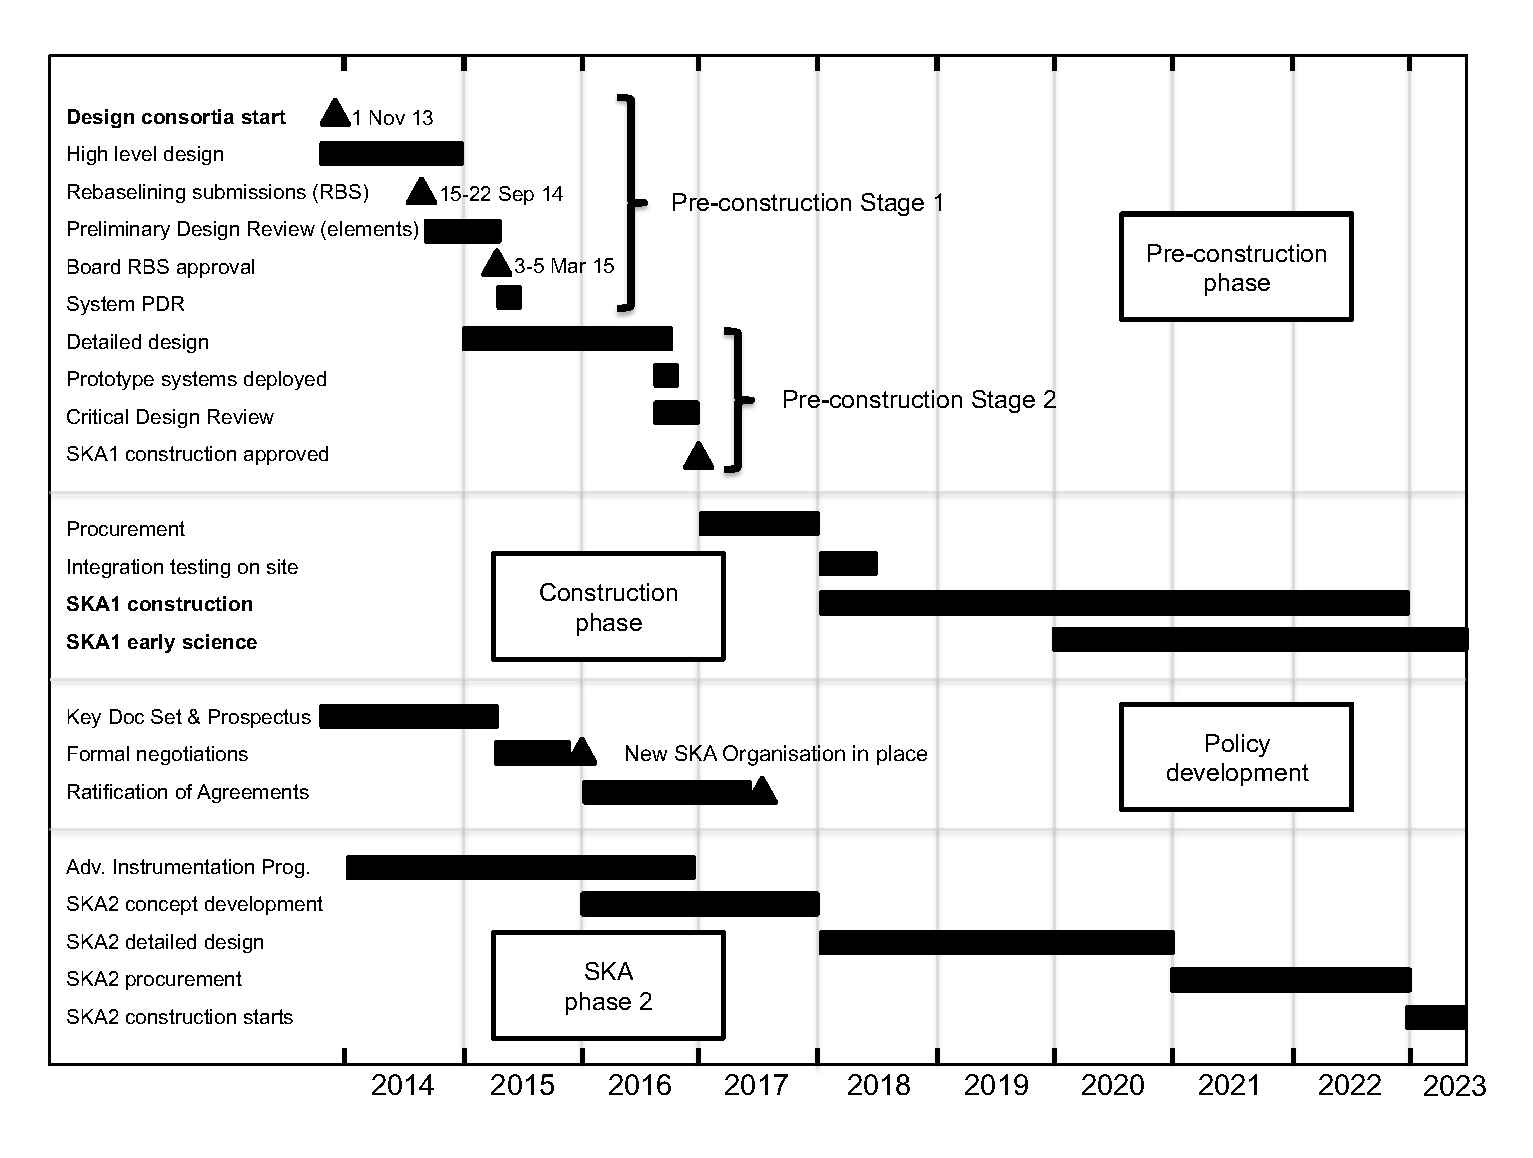
\includegraphics[width=\linewidth]{introduction/c01.s2.f1.eps}
\caption{SKA計画のスケジュール(Alistair McPhersonならびにRobert Braun提供)。}\label{c01.s2.f1}
\end{center}
\end{figure}

\paragraph{国際SKAサイエンスブック2015} 

2004年に出版された国際SKAサイエンスブック2004から10年が経過したことを受けて、2014年度にサイエンスブックの刷新が図られている。そのサイエンスの内容を検討する国際会議が2014年6月にイタリアで開催され、同12月までにはサマリー章を除く論文が採録決定された。すでに多くの論文がarXivに投稿されている。このサイエンスブックの刷新はRBSとは独立しているため、仮に一部の論文が基本デザインの修正と整合しない場合でもそのまま出版される。SKAOはRBSの結果に対するコメントを最終的に載せて、2015年の春に出版をする予定である。本書では、この国際SKAサイエンスブック2015について重点的に触れる。本書で特に断りなく「国際サイエンスブック」と称した場合、この刷新された版を指す。

\paragraph{優先的な科学目標}

前小節ではSKAの主要な科学を紹介したが、デザイン設計やデザイン設計の修正の過程においては、その都度優先的な科学目標が定義されてきた。例えば、2013年3月にSKA1 Baseline Designが設計された際には、宇宙再電離がメートル波の、パルサーがセンチ波の中核的な科学目標と定義づけられた。2014年度のRBSの過程においては、13の具体的な観測プランまで伴った最優先科学目標(Highest Priority Science Objectives、HPSOs)が参照された。
しかし、SRPやSEACの諮問においては、引き続き宇宙再電離とパルサーがSKA1の中核的な科学目標だという認識もあった。


%%%%%%%%%%%%%%%%%%%%%%%%%%%%%%%%%%%%%%%%%%%%%%%
%%%%%%%%%%%%%%%%%%%%%%%%%%%%%%%%%%%%%%%%%%%%%%%
\subsection{今後について}
\label{c01.s2.ss4}

\paragraph{主要科学観測計画} 

SKAはその構想段階においては、SKAメンバー国・非メンバー国の如何を問わず、世界中の研究者が観測に参加でき成果を得ることができるというオープンスカイポリシーを持っていた。しかし、現在はそのポリシーは大幅に変更されている。SKA1においては、観測可能時間の半分以上が長時間の観測プログラムで構成される主要科学計画(Key Science Programs、KSP)に配分される。KSPはSKAメンバー国の研究者でなければ代表を務めることはできない見込みである。そしてKSPから生み出される成果もSKAメンバー国の研究者のものとなる。非メンバー国の研究者が主体となる(例えば論文の筆頭著者になる)のは難しい見通しである。一般公募の観測時間はごくわずかのため、高い競争率が予想される。ゆえにSKAメンバー国とならずとも観測時間が得られると考えるのは早計である。なお、2015年8月にストックホルムにて、このKSPについて意見交換を行う国際会議が開催される。

\paragraph{仮デザイン審査(PDR)を経て詳細設計へ} 

2014年度後半から、SKAOは各コンソーシアムから提案されたシステムや要素レベルでの設計案を順次審査している。この仮デザイン審査(Preliminary Design Review、PDR)後、有望なものがコンソーシアム内で絞り込まれ、詳細設計へと移行される予定である。2015年3月に決定される基本デザインの修正は、程度の差こそあれ仮デザイン審査の追加を必要とするだろう。ただし、基本デザインの修正はすでに存在する要素設計案から経費削減できる修正を絞り込むという方法をとっている。従って要素レベルで全面的な仮デザイン審査のやり直しということは起こらない。スケジュールに与える影響は限定的である。


%%%%%%%%%%%%%%%%%%%%%%%%%%%%%%%%%%%%%%%%%%%%%%%
%%%%%%%%%%%%%%%%%%%%%%%%%%%%%%%%%%%%%%%%%%%%%%%
%%%%%%%%%%%%%%%%%%%%%%%%%%%%%%%%%%%%%%%%%%%%%%%
\setcounter{section}{2}\section{我が国のSKA計画の歩み}
\label{c01.s3}

%%%%%%%%%%%%%%%%%%%%%%%%%%%%%%%%%%%%%%%%%%%%%%%
%%%%%%%%%%%%%%%%%%%%%%%%%%%%%%%%%%%%%%%%%%%%%%%
\subsection{これまでの活動状況}
\label{c01.s3.ss1}

\paragraph{我が国の参加の意義}

我が国がこのような世界規模の計画に金銭的・技術的に参画することは、イニシアチブを確保して研究を有利に進めるだけでなく、計画を通じた科学・技術の発展や人材の育成に大きな意義をもつ。世界中の研究者が英知を結集してSKA計画を進めている中で、科学・技術の先進国として、日本が世界から大きな期待を持たれていることも事実である。日本学術会議はその提言「第22期学術の大型研究計画に関するマスタープラン2014」の中で重点大型研究計画としてSKAを選んでいる。

\paragraph{日本SKAコンソーシアム}

日本では2008年に日本SKAコンソーシアム(SKA-JP)が結成され、 研究者レベルでの活動が行われている。現在160名を超える科学者・技術者が参加している。運営はコンソーシアム代表(杉山直、名古屋大学)と副代表(中西裕之、鹿児島大学、ならびに市來浄與、名古屋大学)、資金獲得担当(今井裕、鹿児島大学)ならびに広報担当(市來浄與、名古屋大学)が担っている。活動の中核は次に紹介するSKA-JP科学検討班が担っている。また技術開発を目指すSKA-JP技術検討班や産業界と連携をするための産業フォーラムも組織されている。

\paragraph{科学検討班}

SKA-JPには科学検討班が設置され、SKA計画に関する様々な活動の中核を成している。運営は代表(高橋慶太郎、熊本大学)と副代表(竹内努、名古屋大学)が担っている。科学検討班は次の6組織あり、高赤方偏移については本書執筆のため3グループを形成した。
\begin{itemize}
\item[★] 高赤方偏移(代表:平下博之、ASIAA)
\begin{itemize}
\item[●] 宇宙論(代表:山内大介、東京大学)
\item[●] 再電離(代表:市來淨與、名古屋大学)
\item[●] 銀河進化(代表:竹内努、名古屋大学)
\end{itemize}
\item[★] パルサー(代表:高橋慶太郎、熊本大学)
\item[★] 宇宙磁場(代表:赤堀卓也、鹿児島大学)
\item[★] 位置天文(代表:今井裕、鹿児島大学)
\item[★] 星間物質(代表:半田利弘、鹿児島大学)
\item[★] 突発天体(代表:青木貴弘、早稲田大学)
\end{itemize}
それぞれの組織は数10名程度のメンバーによって構成され、自立的に活動をしている。本書の執筆は各科学検討班メンバーらが行った。著者一覧を各章の末尾に掲載する。なお、SKA-JPの設立後早期から活動を蓄積している班もあれば、本書の執筆のために数ヶ月前に結成された班もある。そのため章ごとに検討進度にかなりの違いがあることを予めご理解頂きたい。

%%%%%%%%%%%%%%%%%%%%%%%%%%%%%%%%%%%%%%%%%%%%%%%
%%%%%%%%%%%%%%%%%%%%%%%%%%%%%%%%%%%%%%%%%%%%%%%
\subsection{本書について}
\label{c01.s3.ss2}

\paragraph{編纂の経緯}

本書の製作には3つの目的がある。1つ目に、我が国のSKA計画への参入について学会的議論を醸成するために、非専門家、たとえば電波天文学を専門としない科学者や若手研究者にもSKAの科学的課題の本質を理解して頂く目的がある。その達成のために、本書ではSKAによって解明を目指す課題の基礎を比較的丁寧にまとめた。2つ目に、SKA計画においては日本は後発にあるため、世界の情勢を把握する目的がある。特にSKA計画の可能性と実現性を見定める目的がある。その達成のために、本書では国際SKAサイエンスブック2015の内容を紹介した。3つ目に、日本がSKA計画に参加した場合の意義を明確にする目的がある。その達成のために、本書では我が国がSKAで果たせるであろう独自性をまとめた。各章はこれらの3項目をそれぞれ教科書的、総説的、そして白書的にまとめている。

\paragraph{本書の範囲}

SKA計画には多岐にわたる科学目標があるため、その全てを網羅し解説をすることには困難を伴った。日本SKAコンソーシアムには様々な分野の専門家が集まっており、各自が各々の分野の報告をまとめることによって、できるだけ幅広い解説ができるように努めた。しかし、例えば宇宙生命分野など、本書で網羅出来なかった科学的課題もいくつかある。それらについては、出版の予定される国際SKAサイエンスブックをぜひ参照されたい。その他本書の執筆の参考としている主要なSKA文書を表\ref{c01.s3.t1}にまとめた。

\begin{table}
\caption{SKA重要文書一覧とそのリンク}
\begin{center}
\footnotesize
\begin{tabular}{p{48zw}}
\hline\hline
\noalign{\smallskip}
★ Phase 1 Baseline Design: 
\url{http://astronomers.skatelescope.org/ska1/}\\
\noalign{\smallskip}
★ Phase 2 Predicted Design: 
\url{http://astronomers.skatelescope.org/ska2/}\\
\noalign{\smallskip}
★ Phase 1 Concept of Operations (revision B): 
\url{http://astronomers.skatelescope.org/wp-content/uploads/2014/03/SKAConOpsRevB.pdf}\\
\noalign{\smallskip}
★ Phase 1 Science Priority Outcome: 
\url{http://astronomers.skatelescope.org/wp-content/uploads/2014/10/SKA-TEL-SKO-0000122-SCI-REQ-RE-01-SKA1SciencePrioritiesOutcome.pdf}\\
\noalign{\smallskip}
★ Phase 1 Imaging Science Performance: 
\url{http://astronomers.skatelescope.org/wp-content/uploads/2014/06/SKA1_Science_Performance_RevA_draft5.pdf}\\
\noalign{\smallskip}
★ Phase 1 Level 1 (System) Requirements Specification (revision 5): 
\url{http://astronomers.skatelescope.org/wp-content/uploads/2015/02/SKA-TEL-SKO-0000008-AG-REQ-SRS-Rev05-SKA1_Level_1_System_Requirement_Specification-signed.pdf}\\
\noalign{\smallskip}
★ Phase 1 Level 0 (Science) Requirements (latest draft): 
\url{http://astronomers.skatelescope.org/wp-content/uploads/2014/06/SKA1-Level0-Requirements.pdf}\\
\noalign{\smallskip}
★ Phase 1 Scientific Use Cases (latest draft): 
\url{http://astronomers.skatelescope.org/wp-content/uploads/2014/05/SKA-SCI-USE-001-G_Science_use_cases-signed1.pdf}\\
\noalign{\smallskip}
★ SWG Assessment Workshop Summary: Continuum: 
\url{https://indico.skatelescope.org/getFile.py/access?resId=0&materialId=4&confId=261}\\
\noalign{\smallskip}
★ SWG Assessment Workshop Summary: Cosmology: 
\url{https://indico.skatelescope.org/getFile.py/access?resId=0&materialId=3&confId=273}\\
\noalign{\smallskip}
★ SWG Assessment Workshop Summary: Cradle of Life: 
\url{https://indico.skatelescope.org/getFile.py/access?resId=0&materialId=3&confId=266}\\
\noalign{\smallskip}
★ SWG Assessment Workshop Summary: EoR and the Cosmic Dawn: 
\url{https://indico.skatelescope.org/getFile.py/access?resId=0&materialId=2&confId=259}\\
\noalign{\smallskip}
★ SWG Assessment Workshop Summary: HI Galaxy: 
\url{https://indico.skatelescope.org/getFile.py/access?resId=0&materialId=3&confId=262}\\
\noalign{\smallskip}
★ SWG Assessment Workshop Summary: Magnetism: 
\url{https://indico.skatelescope.org/getFile.py/access?resId=0&materialId=1&confId=274}\\
\noalign{\smallskip}
★ SWG Assessment Workshop Summary: Pulsars: 
\url{https://indico.skatelescope.org/getFile.py/access?resId=0&materialId=3&confId=260}\\
\noalign{\smallskip}
★ SWG Assessment Workshop Summary: Transients: 
\url{https://indico.skatelescope.org/getFile.py/access?resId=0&materialId=2&confId=275}\\
\noalign{\smallskip}
★ Phase 1 System Baseline Design (Corrections): 
\url{https://www.skatelescope.org/wp-content/uploads/2014/11/SKA-TEL-SKO-0000002-AG-BD-DD-01-SKA1_System_Baseline_Design_Miscellaneous_Corrections.pdf}\\
\noalign{\smallskip}
★ Phase 1 System Baseline Design (2013 March 12): 
\url{http://www.skatelescope.org/wp-content/uploads/2012/07/SKA-TEL-SKO-DD-001-1_BaselineDesign1.pdf}\\
\noalign{\smallskip}
★ Project Execution Plan: 
\url{http://www.skatelescope.org/uploaded/38221_SKA_Project_Execution_Plan.pdf}\\
\noalign{\smallskip}
★ Phase 1 Design Reference Mission (DRM version 2.0): 
\url{http://www.skatelescope.org/uploaded/18714_SKA1DesRefMission.pdf}\\
\noalign{\smallskip}
★ Phase 2 Design Reference Mission (DRM version 1.0): 
\url{http://www.skatelescope.org/uploaded/3517_DRM_v1.0.pdf}\\
\noalign{\smallskip}
\hline
\end{tabular}\label{c01.s3.t1}
\end{center}
\end{table}

\paragraph{各章の内容}

本書では宇宙再電離 (\S \ref{EoR})、宇宙論 (\S \ref{cosmology})、銀河進化 (\S \ref{galaxy})、パルサー (\S \ref{pulsar})、宇宙磁場 (\S \ref{magnetism})、近傍宇宙時空計測 (\S \ref{astrometry})、星間物質 (\S \ref{ISM})、突発天体 (\S \ref{transients}) のサイエンスについて触れる。




\chapter{宇宙再電離}\label{EoR}

%%%%%%%%%%%%%%%%%%%%%%%%%%%%%%%%%%%%%%%%%%%%%%%
%%%%%%%%%%%%%%%%%%%%%%%%%%%%%%%%%%%%%%%%%%%%%%%
%\setcounter{section}{1}
\section{$BL$2r7h$N%5%$%(%s%9(B}\label{c03.s1}
$B%$%s%U%l!<%7%g%s$K;O$^$j!"%S%C%0%P%s85AG9g@.$r7P$F9b29!"9bL)EY$G%W%i%:%^(B
$B>uBV$@$C$?1'Ch$O(B$z\sim 1100$$B$N:"!"<+M3EE;R$,M[;R$KB*$($i$l!"Cf@-?eAG$,7A(B
$B@.$5$l$?(B($B:F7k9g(B)$B!#$3$l0J9_!"(B$z\sim30$$B$^$G$OE7BN$NB8:_$7$J$$;~Be(B($B0E9u;~Be(B)$B$,(B
$BB3$$$F$$$?$,!"(B$z\sim 30$$B$G=iBeE7BN$N7A@.$,;O$^$j(B(cosmic dawn : CD)$B!"3,AX(B
$BE*9=B$7A@.$K$h$j6d2O!"6d2OCD$HBg5,LO$J9=B$$,7A@.$,?J$_!"8=:_$N1'Ch$X$H;j(B
$B$k!#(B $B$3$N9=B$7A@.$N2aDx$N(B$z\sim 15$$B$G!":FEEN%4|(B(Epoch of Reionization :
EoR)$B$H8F$P$l$k;~Be$,;O$^$k$H9M$($i$l$F$$$k!#$3$l$O!":F7k9g4|0J8e!"Cf@->uBV$GB8:_$7$F$$$?(B
$B?eAG$,!"@1$d6d2O$+$i$N;g30@~(B(UV)$B$d(BX$B@~$K$h$C$FEEN%$r0z$-5/$3$5$l$k8=>]$G(B
$B$"$j!"8=:_$N4QB,$G$O!":FEEN%4|$O(B$z\sim 6$$B$^$GB3$$$?$H9M$($i$l$F$$$k(B
\citep{2006ARA&A..44..415F}$B!#8=:_$G$O:FEEN%$O40N;$7$F$*$j!"6d2OFb$J$I$r=|(B
$B$$$F$O!"1'Ch$NBgItJ,$,EEN%$7$?>uBV$K$"$k!#$3$N>O$G$O<g$K!":FEEN%$,;O$^$C(B
$B$F$+$i40N;$9$k$^$G$N4|4V(B($6\lesssim z\lesssim 15$)$B$KCmL\$9$k!#(B

$B8=:_!"9b@VJ}JP0\$N%/%'!<%5!<$d%,%s%^@~%P!<%9%H(B(GRB)$B!"%i%$%^%s(B$\alpha$$B?9$N4QB,$K$h$C$F!"(BEoR$B=*4|$K$D$$$F$O4QB,$,FO$-$D$D$"$k$,!"(BEoR$B3+;O;~4|(B
$B$d!"$=$N4|4V$K$D$$$F$OL$$@J,$+$C$F$$$J$$!#$7$+$7!"8=:_!"7W2h$,?J9TCf$N(B
Square Kilometer Array (SKA)$B$G$O!"(B$z\sim 27$$B$^$G4QB,$9$k;v$,2DG=$H$J$j!"(B
$B=iBeE7BN$d(BEoR$B$K$D$$$F$N>pJsNL$,HtLvE*$KA}$($k$H4|BT$5$l$F$$$k!#(B

\subsection{$B1'Ch@2$l>e$,$j$+$i0E9u;~Be(B}
$B:F7k9g0JA0$N1'Ch$O!"9b29!"9bL)EY$J%W%i%:%^>uBV$H$J$C$F$$$?$,!"(B
$B1'ChKDD%$KH<$$1'Ch$N29EY$ONd$($F!"M[;R$HEE;R$,7k9g$7Cf@-?eAG$r:n$j;O$a$?!#(B
$B$3$l$K$h$j!"%W%i%:%^Cf$G$N;6Mp$K$h$j$^$C$9$0?J$`;v$N$G$-$J$+$C$?8w;R$O!"(B
$B<+M3$K?J$`;v$,$G$-$k$h$&$K$J$j!":#F|!"1'Ch%^%$%/%mGHGX7JJ|<M(B(CMB)$B$H$7$F4QB,(B
$B$5$l$F$$$k!#$3$N8=>]$r1'Ch@2$l>e$,$j$H8F$S!"=iBeE7BN$,7A@.$5$l$O$8$a(B
$B$k$^$G$N1'Ch$,Cf@-?eAG$GK~$?$5$l$F$$$k;~4|$r0E9u;~Be$H8F$V!#(B

\subsection{$B0E9u;~Be$N=*_a$H:FEEN%4|$N;O$^$j(B}
$B8=:_$NI8=`1'ChO@$NOHAH$_$G$O!"%$%s%U%l!<%7%g%s;~$K:n$i$l$?L)EYMI$i$.$,;~(B
$B4VH/E8$7!"L)EYMI$i$.$NBg$-$$2U=j$G%@!<%/%^%?!<$,=ENO<}=L$7!"Dc<ANL(B
($10^{5-6}M_\odot$)$B%_%K%O%m!<$r7A@.$7$?$H9M$($i$l$F$$$k!#$3$N%_%K%O%m!<Fb(B
$B$G?eAGJ,;R$,7A@.$5$l!"?eAGJ,;RNd5Q$K$h$C$FNd$($?%,%9$,=ENO<}=L$rB3$1$k$3(B
$B$H$G!"=iBe@1$r7A@.$9$k$3$H$,%7%_%e%l!<%7%g%s$G<($5$l$F$$$k(B
\citep{2006ApJ...652....6Y}$B!#6aG/$G$O!"mU<M%U%#!<%I%P%C%/$r9MN8$7$?=iBe(B
$B@17A@.$NmU<MN.BN%7%_%e%l!<%7%g%s$b$J$5$l!"=iBe@1<ANL$N7hDj$K$O!"mU<M%U%#!<(B
$B%I%P%C%/$,=EMW$G$"$k$3$H(B \citep{2011Sci...334.1250H}$B!"%_%K%O%m!<FbIt$N%,(B
$B%9$NFCD'(B($B<ANL!"3Q1?F0NL!"<ANL9_CeN((B)$B$K1~$8$F!"(B$10-1000 M_{\odot}$$B$NI}9-$$(B
$B=iBe@1<ANL$,<B8=$5$l$k;v$,<($5$l$F$$$k(B \citep{2014ApJ...781...60H}$B!#$3$l(B
$B$i=iBe@1$,H/$9$kmU<M$K$h$j0E9u;~Be$O=*_a$9$k!#(B
%$B$^$?!"=iBe@1$K$h$j(BLyman Werner$B8w;R$,J|<M$5$l$k$3$H$K$h$C$F%_%K%O%m!<Fb$N%S%j%"%k29EY(B$T_{{\rm K}}$$B$,(B$10^{4}{\rm K}$$B$rD6$(!"J,;RNd5Q$h$j$b8zN($NNI$$86;RNd5Q$,5/$-$F@1$,8zN(E*$K7A@.$5$l!"$3$l$i$,=iBe6d2O$r7A@.$7$F$$$/(B(\citep{2011ARA&A..49..373B})$B!#(B
$B$3$N8e!"3,AXE*9=B$7A@.$K$h$j%_%K%O%m!<$,9gBN@.D9$9$k$3$H$G$h$j<ANL$NBg$-(B
$B$J=iBe6d2O$,7A@.$5$l$k$H9M$($i$l$k!#(B 

$B:G6a$N4QB,$K$h$k$H!"(B$z=7.085$$B$G<ANL(B$\sim 2\times 10^{9}M_{\odot}$$B$ND65pBg(B
$B%V%i%C%/%[!<%k$,B8:_$7$?;v$,<(:6$5$l$F$*$j(B \citep{2011Natur.474..616M}$B!"(B
$B=iBe@1$d=iBe6d2O$N7A@.$HJB9T$7$F!"D65pBg%V%i%C%/%[!<%k$N7A@.$b?J$s$@$H9M(B
$B$($i$l$k!#(B$z=7.085$$B$NCJ3,$G$3$l$[$IBg<ANL$K%V%i%C%/%[!<%k$r@.D9$5$;$k2aDx(B
$B$OL$$@ITL@$G$"$j!"MM!9$J%7%J%j%*$,9M$($i$l$F$$$k!#(B

$B=iBe@1$d=iBe6d2O$+$i$O!"Cf@-?eAG$rEEN%$5$;$k$N$KI,MW$J(B13.6${\rm eV}$$B$h$j(B
$B$bBg$-$J%(%M%k%.!<$r;}$C$?mU<M$KJ|<M$5$l!"1'Ch:FEEN%$N;~Be$,;O$^$C$?$H9M(B
$B$($i$l$k$,!"1'Ch:FEEN%$N>\:Y$K$D$$$F$O4QB,E*$K$O$^$C$?$/L$2rL@$G$"$k!#$3(B
$B$l$i=iBeE7BN$r(BSKA$B$GD>@\4QB,$9$k$3$H$OFq$7$$$,!"=iBe@1$N=i4|<ANL4X?t$d7A@.(B
$BN(!"$*$h$S=iBe6d2O$+$i$N8w;RC&=P3NN($J$I$N>pJs$O!"$3$l$i$r>\:Y$K%b%G%k2=(B
$B$7$FEEN%9=B$$NH/E8$r7W;;$74QB,$HHf3S$9$k$3$H$G4V@\E*$KF@$k$3$H$,2DG=$G$"(B
$B$m$&!#$^$?!"%V%i%C%/%[!<%k$K$D$$$F$=$N9_Ce1_HW$+$iH/$;$i$l$k(BX$B@~$O6d2O4V%,(B
$B%9$N2CG.$rDL$8$F$d$O$jEEN%9=B$$NH/E8$K1F6A$r$*$h$\$9!#:FEEN%$rD>@\E*$KC5(B
$B$k$3$H$,K>$^$l$F$*$j!"$3$l$r2DG=$K$9$k$N$,0J2<$K=R$Y$k(B21cm$B@~$K$h$k:FEEN%(B
$B4|$N4QB,$G$"$k!#(B

\subsection{21cm$B@~(B}
$B=iBeE7BN7A@.$d(BEoR$B$rC5$k8z2LE*$JJ}K!$H$7$F!"Cf@-?eAG$ND6Hy:Y9=B$M3Mh$N(B
21cm$B@~$,$"$k(B \citep{2006PhR...433..181F}$B!#:FEEN%$,;O$^$kA0$+$i:FEEN%=i4|(B
$B$K$OCf@-?eAG$,BgNL$KB8:_$7$F$$$?$?$a!"(B21cm$B@~$r4QB,$9$k;v$K$h$C$F!"$3$l$i(B
$B$N;~4|$rD>@\C5$k$3$H$,$G$-$k!#4QB,NL$H$7$F$O!"%9%T%s29EY$H(BCMB$B$N29EY(B $T_{{\gamma}}$$B$H$N:9$GDj5A$5$l$k51EY29EY$,<0(B
$B!J(B$\ref{eq:brightness}$$B!K$GM?$($i$l$k!#(B
\begin{align}
\delta T_{{\rm b}}(\nu) &=\frac{T_{{\rm S}}-T_{{\gamma}}}{1+z}(1-e^{-\tau_{\nu_{0}}})\notag \\ 
&\sim27 x_{{\rm H\textsc{i}}}(1+\delta)\bigg(1-\frac{T_{\gamma}}{T_{s}}\bigg)\bigg(\frac{H}{dv_{||}/dr_{||}}\bigg)\bigg(\frac{1+z}{10}\bigg)^{1/2}\bigg(\frac{0.15}{\Omega_{m}h^{2}}\bigg)^{1/2}\bigg(\frac{\Omega_{b}h^{2}}{0.023}\bigg) [{\rm mK}]
\label{eq:brightness}
\end{align}
$B$3$3$G!"51EY29EY$O;k@~J}8~$G7W;;(B
$B$5$l$kNL$G$"$j!"(B$\tau_{\nu_{0}}$$B$OGHD9(B21cm$B$KAjEv$9$k<~GH?t(B
$\nu_{0}$$B!J(B$=1.4$ GHz$B!K$G$N8w3XE*8|$5$G!"(B
\begin{eqnarray}
\tau_{\nu_0}(z)&=&\frac{3}{32\pi}\frac{h_{p}c^{3}A_{21cm}}{k_{{\rm B}}\nu_{0}^{2}}\frac{n_{{\rm H}}}{T_{{\rm S}}(1+z)dv_{||}/dr_{||}} \notag\\
&=&9.6\times 10^{-3}(1+\delta)\left(\frac{1+z}{10} \right)^{3/2}\left(\frac{x_{{\rm H\textsc{i}}}}{T_{{\rm S}}}\right)\left[\frac{H(z)/(1+z)}{dv_{||}/dr_{||}}\right]
\label{eq:optical}
\end{eqnarray}
$B$HI=$5$l$k!#>e<0$K$*$$$F!"(B$n_{{\rm H}}$$B$O?eAG$N?tL)EY!"(B$\delta$$B$O%,%9$ND6(B
$B2aL)EY!"(B$x_{{\rm H\textsc{i}}}$$B$OJ?6QCf@-?eAGN(!"(B$T_{{\rm S}}$$B$O%9%T%s29(B
$BEY!"(B$\Omega_mh^2$$B!"(B$\Omega_bh^2$$B$O$=$l$>$l%@!<%/%^%?!<!"%P%j%*%s$NL)EY%Q(B
$B%i%a%?!<$G$"$k!#(B
$B$^$?!"(B$A_{21}=2.85\times 10^{-15}$s$^{-1}$$B$O%"%$%s%7%e%?%$%s(B$A$$B78?t!"(B$H$
$B$O%O%C%V%k%Q%i%a!<%?!"(B$dv_{||}/dr_{||}$$B$O%,%9$N;k@~J}8~$NB.EY8{G[$G$"$k!#(B
$BL)EYMI$i$.(B$\delta$$B!"6d2O4V%,%9(B(IGM)$B$NB.EY8{G[(B$dv_{||}/dr_{||}$$B$O1'ChO@E*$K7h(B
$B$^$kJ*M}NL$G$"$k$,!"Cf@-?eAGN((B $x_{{\rm HI}}$$B$H%9%T%s29EY(B $T_{{\rm S}}$$B$O(B
$BE7BNJ*M}3XE*$K7h$^$kNL$G$"$j!"$3$l$i$,(BEoR$B$N>pJs$r4^$s$G$$$k!#(B$\delta
T_{{\rm b}}>0$$B$N$H$-!"51EY29EY$O(BCMB$B$KBP$9$k51@~$H$7$F4QB,$5$l!"(B$\delta
T_{{\rm b}}<0$$B$N$H$-$O(BCMB$B$KBP$9$k5[<}@~$H$7$F4QB,$5$l$k!#%9%T%s29EY$O!"%,(B
$B%9$N1?F03XE*29EY(B$T_{{\rm K}}$$B!"%i%$%^%s(B$\alpha$$B?'29EY(B$T_{\alpha}$$B!"$=$l$>(B
$B$l$N7k9gDj?t(B$x_{{\rm K}},x_{\alpha}$$B$rMQ$$$F<!$N$h$&$K=q$-I=$9;v$,$G$-$k!#(B
\begin{equation}
T_{{\rm S}}^{-1}=\frac{T_{{\gamma}}^{-1}+x_{\alpha}T_{\alpha}^{-1}+x_{{\rm K}}T^{-1}_{{\rm K}}}{1+x_{\alpha}+x_{{\rm K}}}
\end{equation}
$B$9$J$o$A!"%9%T%s29EY$OCf@-?eAG%,%9$H0J2<$N#3$D$NAj8_:nMQ$K$h$C$F7hDj$5$l(B
$B$k!#(B
\begin{itemize}
 \item[(a)] CMB$B8w;R$H$NAj8_:nMQ(B
 \item[(b)] $B%i%$%^%s(B$\alpha$$B8w;R$H$NAj8_:nMQ(B
 \item[(c)] $BCf@-?eAGF1;N$N>WFM$K$h$kAj8_:nMQ(B
\end{itemize}
$BE7BN7A@.$J$I$N1F6A$O!"(B(2),(3)$B$K$h$kAj8_:nMQ$rDL$8$F%9%T%s29EY$K8=$l$k!#(B

\subsection{$BG.?J2=$NNr;K(B $B!ABg6IE*$J%7%0%J%k!A(B}
IGM$B$NBg6IE*$J%7%0%J%k(B($B@VJ}JP0\Kh$NJ?6QE*$J(BIGM$B$N29EY(B)$B$O3F;~Be$K$D$$$FMM!9(B
$B$JJ*M}5!9=$,F/$-!"0J2<$NMM$JH/E8$r$9$k(B \citep{2011MNRAS.411..955M}$B!#(B

\medskip

\subsubsection{(1) $z\gtrsim 100$, $T_{{\rm K}}=T_{{\rm S}}\le
T_{\gamma}$ ($B>WFM$K$h$k%+%C%W%j%s%04|(B)} 
$z\sim 140$$B$N;~4|$K(BCMB$B8w;R$HEE;R$N%3%s%W%H%s;6Mp$,@Z$l$k!#(B
$B$=$N8e$O!"?eAG86;RF1;N$N>WFM$,;YG[E*$K$J$j!"%9%T%s29EY$O(BIGM$B$N%,%929EY$H(B
$B%+%C%W%j%s%0$9$k!#(BCMB$B8w;R$N29EYJQ2=$N@VJ}JP0\0MB8@-$O(B$(1+z)$$B$KHfNc$9$k$,!"(B
$B%,%929EY$O(B$(1+z)^{2}$$B$KHfNc$9$k$?$a!"(BCMB$B8w;R$N29EY$h$j$b!"%,%929EY$NJ}$,!"(B
$B1'Ch$N?J2=$H6&$K5^7c$K8:>/$9$k!#(B


\subsubsection{(2) $35\lesssim z\lesssim 100$, $T_{\rm K}<T_{{\rm
S}}<T_{\gamma}$ ($B>WFM$K$h$k%+%C%W%j%s%0$,@Z$l$k:"(B)}
$B1'ChKDD%$K$h$C$F(BIGM$B$NL)EY$,8:>/$9$k$H!"?eAG86;RF1;N$N>W(B
$BFM$K$h$k%+%C%W%j%s%0$rJ]$F$J$/$J$j!"%9%T%s29EY$O%,%929EY$+$iC&7k9g$7$F:F(B
$B$S(BCMB$B8w;R$N29EY$K6a$E$/!#(B


\subsubsection{(3) $z\sim 35$, $T_{\rm K}<T_{{\rm
S}}\sim T_{\gamma}$ ($B>WFM$K$h$k%+%C%W%j%s%0$,@Z$l$?8e(B)}
$B>WFM$K$h$k%+%C%W%j%s%0$,@Z$l$?8e$O!"(BIGM$B$N%,%929EY$O(B
CMB$B8w;R$H%+%C%W%j%s%0$9$k$?$a!"$3$NFs$D$N29EY$O$[$\Ey$7$/$J$k!#$b$7!"E7BN(B
$B$,B8:_$;$:!"%i%$%^%s(B$\alpha$$B8w;R$,J|<M$5$l$F$$$J$1$l$P!"%9%T%s29EY$O!"$3(B
$B$N$^$^(BCMB$B8w;R$N29EY$H%+%C%W%j%s%0$7$?>uBV$G8:>/$7$F$$$/!#$7$+$7!"<B:]$K$O!"(B
$B=i4|E7BN$,7A@.$5$l$k$?$a!"$=$&$O$J$i$J$$!#(B

\subsubsection{(4) $25\lesssim z \lesssim 35$, $T_{\rm K}<T_{{\rm
   S}}<T_{\gamma}$B"*(BT_{\rm K}\simeq T_{{\rm S}}<T_{\gamma}$ (Wouthuysen-Field
   $B%+%C%W%j%s%04|(B)}$B=i4|E7BN$,7A@.(B
$B$5$l!"%i%$%^%s(B$\alpha$$B8w;R$,J|<M$5$l$k$H!"(BWouthuysen-Field (WF)$B8z2L$K$h$C(B
$B$F%9%T%s29EY$O:F$S!"%,%929EY$H$N%+%C%W%j%s%0$r;O$a$k!#%i%$%^%s(B$\alpha$$B8w(B
$B;R$O!"%9%T%s29EY$K1F6A$rM?$($k$@$1$G$O$J$/!"(BIGM$B$N2CG.$K$b4sM?$7$F$*$j!"(B
$B%9%T%s29EY$O%,%929EY$K6a$E$/!#$=$N$?$a!"(B$T_{\rm K}\simeq T_{{\rm S}}$$B$H(B
$B$J$k!#(B

\begin{figure}[t]
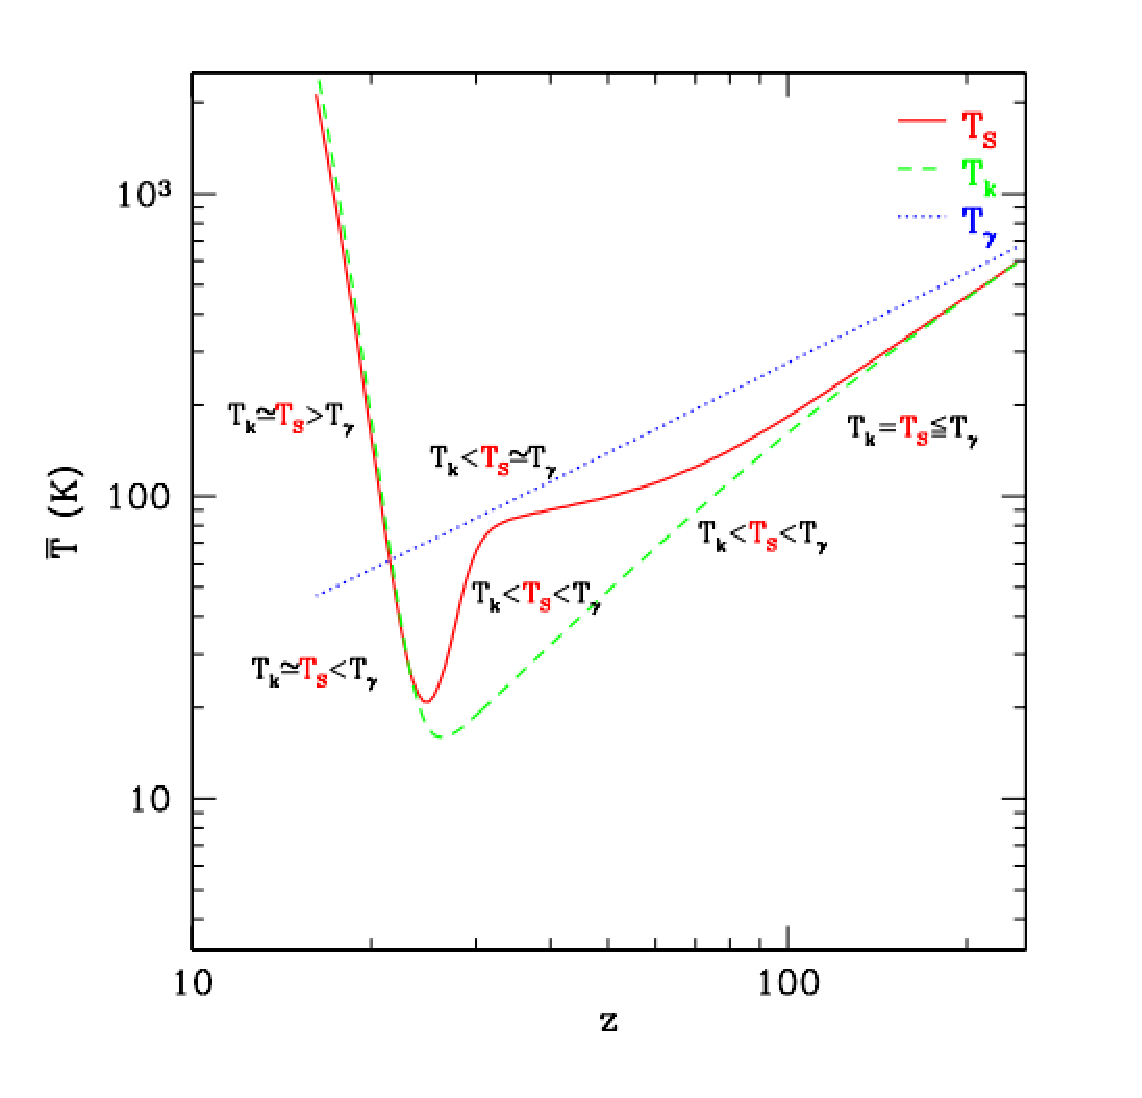
\includegraphics[width=90mm]{EoR/c03/c03.s1.f1.eps}
\centering
\caption{IGM$B29EY$N;~4V?J2=(B(\citep{2011MNRAS.411..955M})$B!#2#<4$O@VJ}JP0\!"=D<4$O29EY$rI=$9!#@V$$<B@~$O%9%T%s29EY!"NP$NGK@~$O%,%929EY!"@D$$E@@~$O(BCMB$B$N29EY$rI=$9!#(B}
\label{fig:igm_history}
\end{figure}

\begin{figure}[!h]
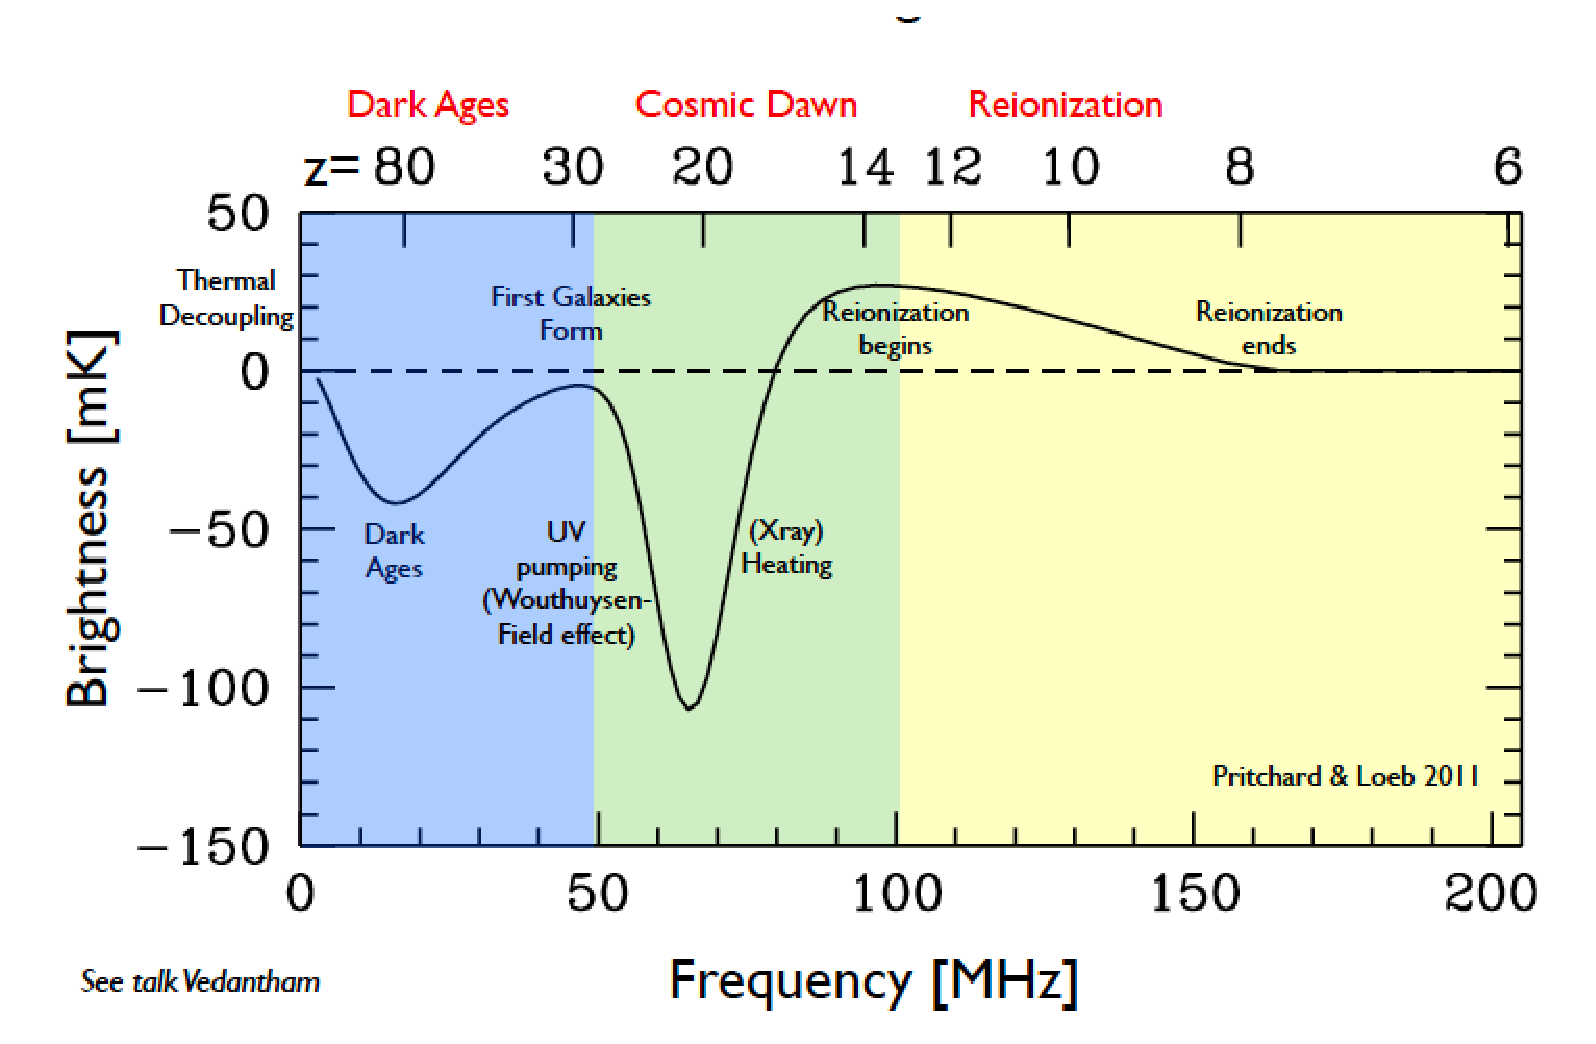
\includegraphics[width=105mm]{EoR/c03/c03.s1.f2.eps}
\centering
\caption{$B51EY29EY$N;~4VH/E8!J(BPritchard \& Loeb, 2011)$B!#2#<4$O<~GH?t!"=D(B
 $B<4$O51EY29EY!#(B$z\lesssim 30$$B$G=i4|E7BN$,7A@.$5$l$k$H!"$=$3$+$iH/$;$i$l(B
 $B$k;g308w$K$h$C$F(BWF$B8z2L$,5/$3$j!"%9%T%s29EY$O(BIGM$B$N%,%929EY$H%+%C%W%j%s%0(B
 $B$9$k!#$3$N$H$-!"%,%929EY$O(BCMB$B$N29EY$h$j>.$5$$$N$G!"51EY29EY$O5[<}@~$H$7(B
 $B$F8+$($k!#$7$+$7!"(B$z\sim 20$$B$G(BX$B@~$K$h$k2CG.$,8z$-;O$a$k$H!"%,%929EY$O5^(B
 $B7c$K>e>:$9$k$?$a!"(B$z\lesssim 15$$B$G$O!"51EY29EY$O51@~$H$7$F4QB,$5$l$k!#$^$?$3$N;~4|!":FEEN%$,;O$^$k!#(B$z\sim 8$$B$K$J$k$H!":FEEN%$,=*$o$j!"Cf@-?eAG$N3d9g$,#0$H$J$k$?$a!"51EY29EY$O<0(B(\ref{eq:brightness})$B$h$j#0$H$J$j!"51@~$b5[<}@~$b8+$($J$/$J$k!#(B}
\label{fig:delta_T}
\end{figure}

\subsubsection{(5) $16\lesssim z \lesssim 25$, $T_{\rm K}=T_{{\rm
S}}<T_{\gamma}$B"*(BT_{\rm K}=T_{{\rm S}}>T_{\gamma}$ (X$B@~$K$h$k2CG.4|(B)} 
WF$B8z2L(B
$B$K$h$j!"%,%9$N%9%T%s29EY$H%,%929EY$O6/$/%+%C%W%k$7$F$$$k$?$a!"1'ChKDD%$H(B
$B6&$K$=$NCM$O8:>/$7$F$$$/$,!"(BX$B@~$K$h$k2CG.$,8z$-;O$a$F$/$k$H!"NO3XE*29EY(B
$B$H%+%C%W%k$7$?%9%T%s29EY$O:G>.$NCM$KC#$7$?8e!"5^7c$J>e>:$r;O$a$k!#$3$N$H(B
$B$-!"1'Ch$NG.?J2=$NCf$G!"(BIGM$B$N29EY$,=i$a$F(BCMB$B8w;R$N29EY$h$j$b==J,Bg$-$/$J(B
$B$k$?$a!"(B$\delta T_{{\rm b}}>0$$B$G$"$k!#$7$?$,$C$F!"(BX$B@~$K$h$k2CG.0JA0$O!"(B
$B51EY29EY$NMI$i$.$O(BCMB$B8w;R$N29EY$KBP$9$k5[<}@~$H$7$F4QB,$5$l$k$,!"(BX$B@~2CG.(B
$B$,8z$-;O$a$k$H51@~$H$7$F4QB,$5$l$k;v$K$J$k!#(B


\subsubsection{(6) $7\lesssim z \lesssim 16$, $T_{\rm K}=T_{{\rm S}}\gg
   T_{\gamma}$ ($B:FEEN%4|(B)}
X$B@~$K(B
$B$h$k2CG.$,==J,$K8z$/$H!"<0!J(B\ref{eq:brightness}$B!K$h$j!"(B$\delta T_{{\rm
b}}$$B$O%9%T%s29EY$K0M$i$J$/$J$j!"29EY0MB8@-$r;}$?$J$/$J$k!#=i4|E7BN$+$i=P(B
$B$F$/$k%$%*%s2=%(%M%k%.!<$h$j$bBg$-$J%(%M%k%.!<$r;}$C$?8w;R$K$h$j!":FEEN%(B
$B$,;O$^$k$H!"%$%*%s2=NN0h!J(BHII$BNN0h!K$,A}$($F$$$-!"Cf@-?eAG$,@j$a$kNN0h(B
$B!J(BHI$BNN0h!K$O=y!9$K8:$C$F$$$/!#$3$l$K$h$j!"Cf@-?eAG$NNL$,8:>/$9$k$?$a!"(B
21cm$B@~$N%7%0%J%k$b8:>/$7$F$$$/!#:FEEN%4|$O!"(BHII$BNN0h$N?J2=$N;EJ}$d!"%$%*(B
$B%s2=8w;R$N?6$kIq$$!"%$%*%s2=8w;R$NJ|<M8;$N?6$kIq$$$J$I$K0MB8$9$k$N$G!"$3(B
$B$l$i$NFCD'$rD4$Y$kI,MW$,$"$k!#(B


$B0J>e!"(B(1)$B$+$i(B(6)$B$K<($7$?$N$,!"(BIGM$B29EY?J2=$N%"%&%H%i%$%s$G$"$j!"(BIGM$B29EY$O(B
$B?^(B\ref{fig:igm_history}$B$K<($9MM$J?6$kIq$$$r$9$k!#$^$?!"<B:]$N4QB,NL$G$"(B
$B$k51EY29EY(B($B<0(B\ref{eq:brightness})$B$N;~4VH/E8$r?^(B\ref{fig:delta_T}$B$K<($9!#(B
$B!!(B

\subsection{WF$B8z2L(B, X$B@~2CG.(B, $B:FEEN%$N%=!<%9(B}
$B$3$N@a$G$O!"(BWF$B8z2L!"(BX$B@~$K$h$k2CG.!":FEEN%$r0z$-5/$3$9E7BN$K$D$$$F=R$Y$k!#(B

\subsubsection{(1)$B<oB2(BIII$B@1(B $\&$ $B<oB2(BII$B@1(B}

$z\sim 30$$B$G!"=E85AG$r4^$^$:!"?eAG$GBgItJ,$,9=@.$5$l$?1'Ch:G=i$N@1$,7A@.(B
$B$5$l;O$a$k(B \citep{2006ApJ...652....6Y}$B!#$3$N$h$&$J?eAG86;R$N$_$G9=@.$5$l(B
$B$?@1$r<oB2(BIII$B@1$H8F$V!#6aG/$N%7%_%e%l!<%7%g%s$K4p$E$/8&5f$K$h$j!"<oB2(BIII
$B@1$O!"(B $BB@M[<ANL$N?t(B10$BG\DxEY$N<ANL$r;}$D$H9M$($i$l$F$$$k(B
\citep{2013RPPh...76k2901B}$B!#$3$N<oB2(BIII$B@1$+$iJ|<M$5$l$k%i%$%^%s(B$\alpha$
$B8w;R$K$h$C$F!"?eAG$N%9%T%s29EY$O%,%929EY$H%+%C%W%j%s%0$9$k!J(BWF$B8z2L!K!#<o(B
$BB2(BIII$B@1$+$i:n$i$l$k(BX$B@~O"@1$O!"(BIGM$B$N2CG.$rC4$&$b$N$H9M$($i$l$F$$(B $B$k(B
\citep{2014MNRAS.445..213F}$B!#$^$?!"<oB2(BIII$B@1$d>/NL$N=E85AG$r4^$`%,%9$+$i(B
$B7A@.$5$l$?<oB2(BII$B@1$,:FEEN%$r0z$-5/$3$9$H4|BT$5$l$F$$$k$,!"<oB2(BIII$B@1$N7A(B
$B@.2aDx!"$=$N8e$N<oB2(BII$B@17A@.%b!<%I$X$NA+0\2aDx$OL$$@Ff$,B?$$!#(B


\subsubsection{(2)Mini-quasar $\&$ AGN}
IGM$B$N2CG.$d:FEEN%$r0z$-5/$3$98w;R$N6!5k$N8;$H$7$F9M$($i$l$k$b$N$H$7$F!"(B
$BCf4V<ANL%V%i%C%/%[!<%k!J(BIMBH$B!K$d!"(BIMBH$B$X$N%,%9$N9_Ce$r5/8;$H$7$?(B
mini-quasar$B$,$"$k(B \citep{2007MNRAS.375.1269Z}$B!#$3$l$iE7BN$K$h$C$F0z$-5/(B
$B$3$5$l$k2CG.$d:FEEN%$O!"@1$+$i$N4sM?$KHf$Y$k$H>.$5$$$,!"(BCMB$B$N29EY$h$j$b(B
$B9b$$29EY$K(BIGM$B$r2CG.$9$k$N$K==J,$J%(%M%k%.!<$r;}$C$?8w;R$r@8@.$9$k$b$N$H(B
$B9M$($i$l$F$$$k!#$^$?!"(BIMBH$B$O8=:_$ND65pBg%V%i%C%/%[!<%k(B(SMBH)$B$N<o$K$J$C$F(B
$B$$$k2DG=@-$b$"$k$,!"%(%G%#%s%H%s9_CeN($h$j$b(B
$BBg$-$JCM$G9_Ce$r5/$3$5$J$1$l$P!"8=:_!"4QB,$5$l$F$$$k9b@VJ}JP0\$N(BAGN$B$N<A(B
$BNL$r@bL@$G$-$J$$$H$$$&LdBj$,$"$k!#(B

\subsubsection{(3) X-ray binaries}
$BA0=R$NDL$j!"<oB2(BIII$B@1M3Mh$N(BX$B@~O"@1$O(BIGM$B$N2CG.8;$H$7$FM-K>;k$5$l$F$$$k!#(B
$B$7$+$7!"(BX$B@~O"@1$O9b@VJ}JP0\$K$*$$$F!"Bg6IE*$J%9%1!<%k$r2CG.$9$k$N$K==J,(B
$B$J8D?t$,B8:_$7$F$$$?$N$+$H$$$&ITDj@-$,$"$k!#(B


\subsection{$B51EY29EY$rDL$7$?4QB,(B}
21cm$B@~$N4QB,$r9T$&$H$-!"2f!9$,<B:]$K1'ChO@E*!"E7BNJ*M}3XE*>pJs$r3MF@$9$k(B
$B$N$O!"51EY29EY$rDL$7$F$G$"$k!#$3$N>O$G$O!"51EY29EY$+$iF@$i$l$k>pJs$K$D$$(B
$B$F4J7i$K$^$H$a$k!#(B


\subsubsection{$B%Q%o!<%9%Z%/%H%k(B}
$B51EY29EY$NMI$i$.$r<h$j07$&$H$-!"$=$NE}7WNL$H$7$F!"0lHLE*$K9-$/MQ$$$i$l$F(B
$B$$$k$N$O$=$N%Q%o!<%9%Z%/%H%k$G$"$k!#0lHLE*$K%Q%o!<%9%Z%/%H%k$OGH?t$H@VJ}(B
$BJP0\$N4X?t$G$"$j!"%Q%o!<%9%Z%/%H%k$K$O!"51EY29EY$N%9%1!<%kKh$NMI$i$.$H$=(B
$B$N;~4VH/E8$N>pJs$,4^$^$l$F$$$k!#51EY29EY$NMI$i$.$r!"%P%j%*%s$NMI$i$.(B
$\delta_{b}$$B!"%$%*%s2=N($NMI$i$.(B $\delta_{x}$$B!"%i%$%^%s(B$\alpha$$B>l$NMI$i(B
$B$.(B $\delta_{\alpha}$$B!"(BIGM$B$N29EY$NMI$i$.(B$\delta_{T}$$B!"$5$i$KB.EY8{G[$NMI(B
$B$i$.(B $\delta_{\partial v}$$B$H!"3F!9$NMI$i$.$N78?t(B$\beta_{i}$$B$rMQ$$$k$H!"(B
$B<0(B(\ref{eq:fluctuation})$B$NMM$K=q$-2<$9;v$,$G$-$k(B
 \citep{2006PhR...433..181F}$B!#(B
\begin{equation}
\delta_{T_{b}}=\beta_{b}\delta_{b}+\beta_{x}\delta_{x}+\beta_{\alpha}\delta_{\alpha}+\beta_{T}\delta_{T}-\delta_{\partial v}
\label{eq:fluctuation}
\end{equation}
$B$3$NE83+$5$l$?MI$i$.$+$i!"$=$N%Q%o!<%9%Z%/%H%k$O!"(B
\begin{equation}
P_{T_{b}}(k,\mu)=P_{\mu^{0}}(k)+\mu^{2}P_{\mu^{2}}(k)+\mu^{4}P_{\mu^{4}}(k)
\label{eq:powerspectrum}
\end{equation}
$B$H7W;;$5$l$k!#(B$\mu$$B$O;k@~J}8~$HGH?t%Y%/%H%k$N$J$93QEY$NM>89$G$"$k!##19`L\$O!"%P%j%*%s$NMI$i$.!"%$%*%s2=N($NMI$i$.!"%i%$%^%s(B$\alpha$$B>l$NMI$i$.!"(BIGM$B$N29EY$NMI$i$.4V$G$N<+8JAj4X!"Aj8_Aj4X$r$^$H$a$?$b$N$G$"$k!#$9$J$o$A$3$l$O!"MI$i$.$NEyJ}@.J,$K$h$k%Q%o!<%9%Z%/%H%k$G$"$k!JB.EY8{G[$K$h$kMI$i$.$O%U!<%j%(6u4V$G9M$($k$H(B$\delta_{\partial v}$=$-\mu^{2}\delta$$B$H$J$k$?$a!"HsEyJ}E*$JMI$i$.$G$"$k!K!##29`L\$O!"HsEyJ}MI$i$.$G$"$kB.EY8{G[MI$i$.$HEyJ}MI$i$.$H$NAj8_Aj4X$K$h$k%Q%o!<%9%Z%/%H%k$r!"#39`L\$OHsEyJ}MI$i$.$K$h$k<+8JAj4X$K$h$k%Q%o!<%9%Z%/%H%k$rI=$7$F$$$k!#?^(B\ref{fig:igm_history_darkage}$B!"(B\ref{fig:igm_history_reionization}$B$K!"3F!9$N;~Be$N(B$\delta T_{{\rm b}}$$B$N%^%C%W$H%Q%o!<%9%Z%/%H%k$r<($9!#(B
%
\begin{figure}[htbp]
\centering
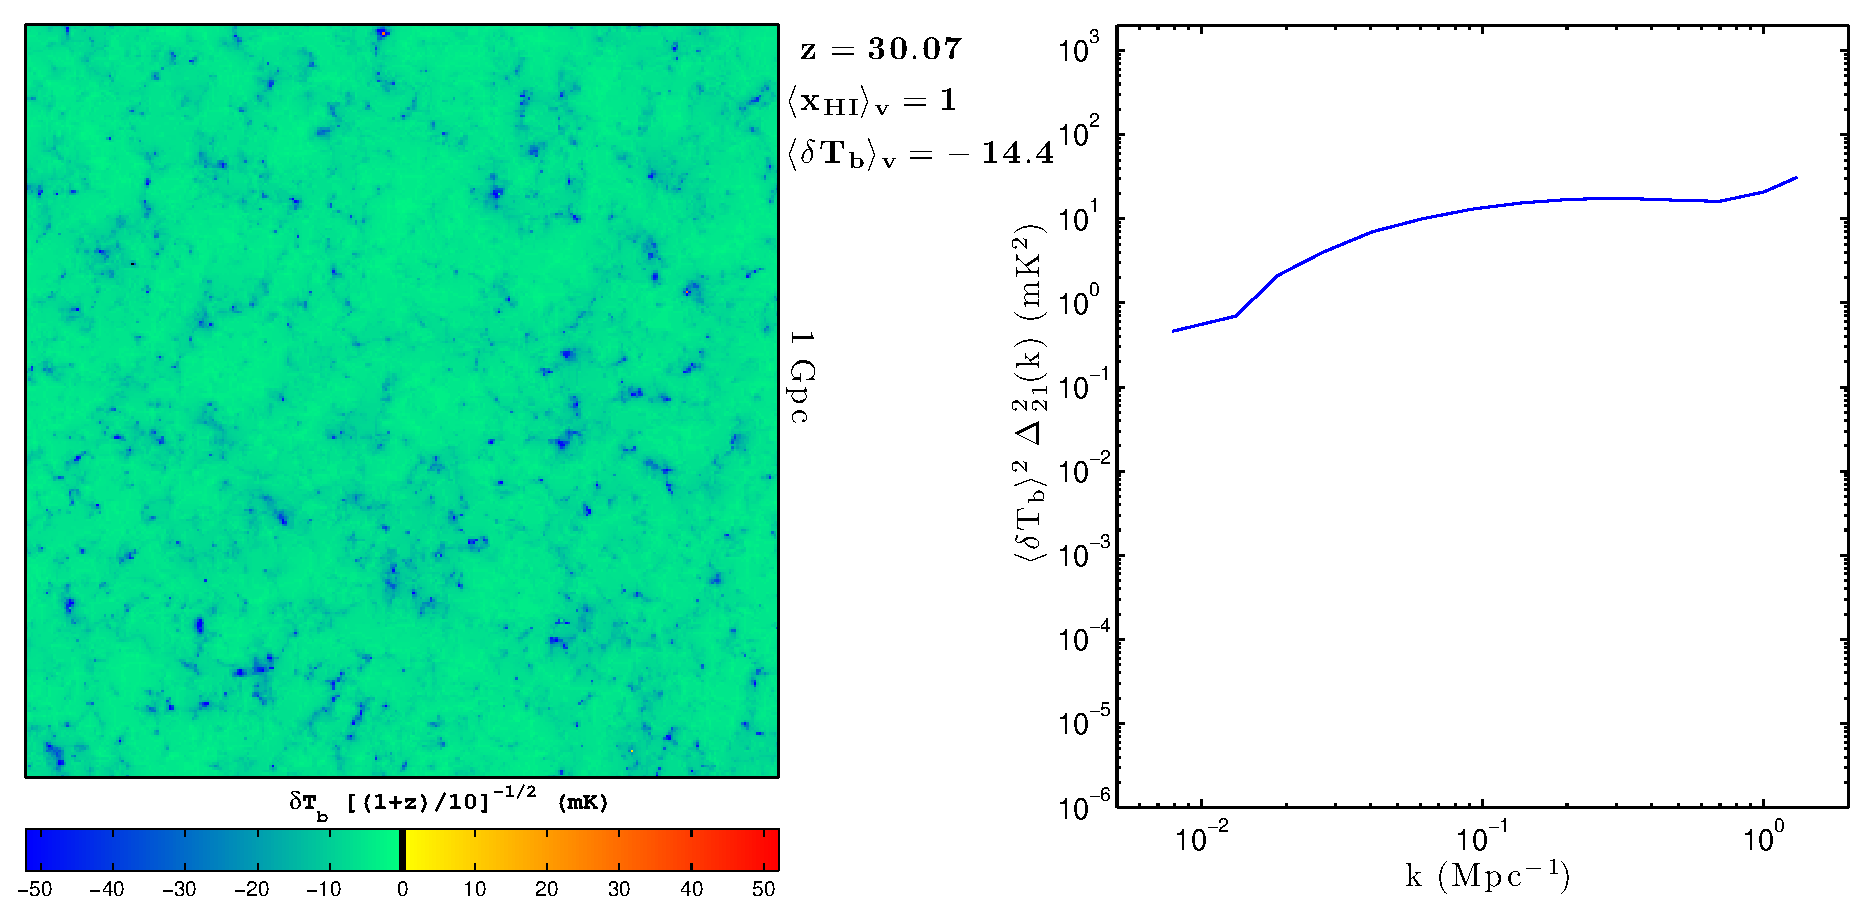
\includegraphics[width=125mm]{EoR/c03/c03.s1.f3a.eps}
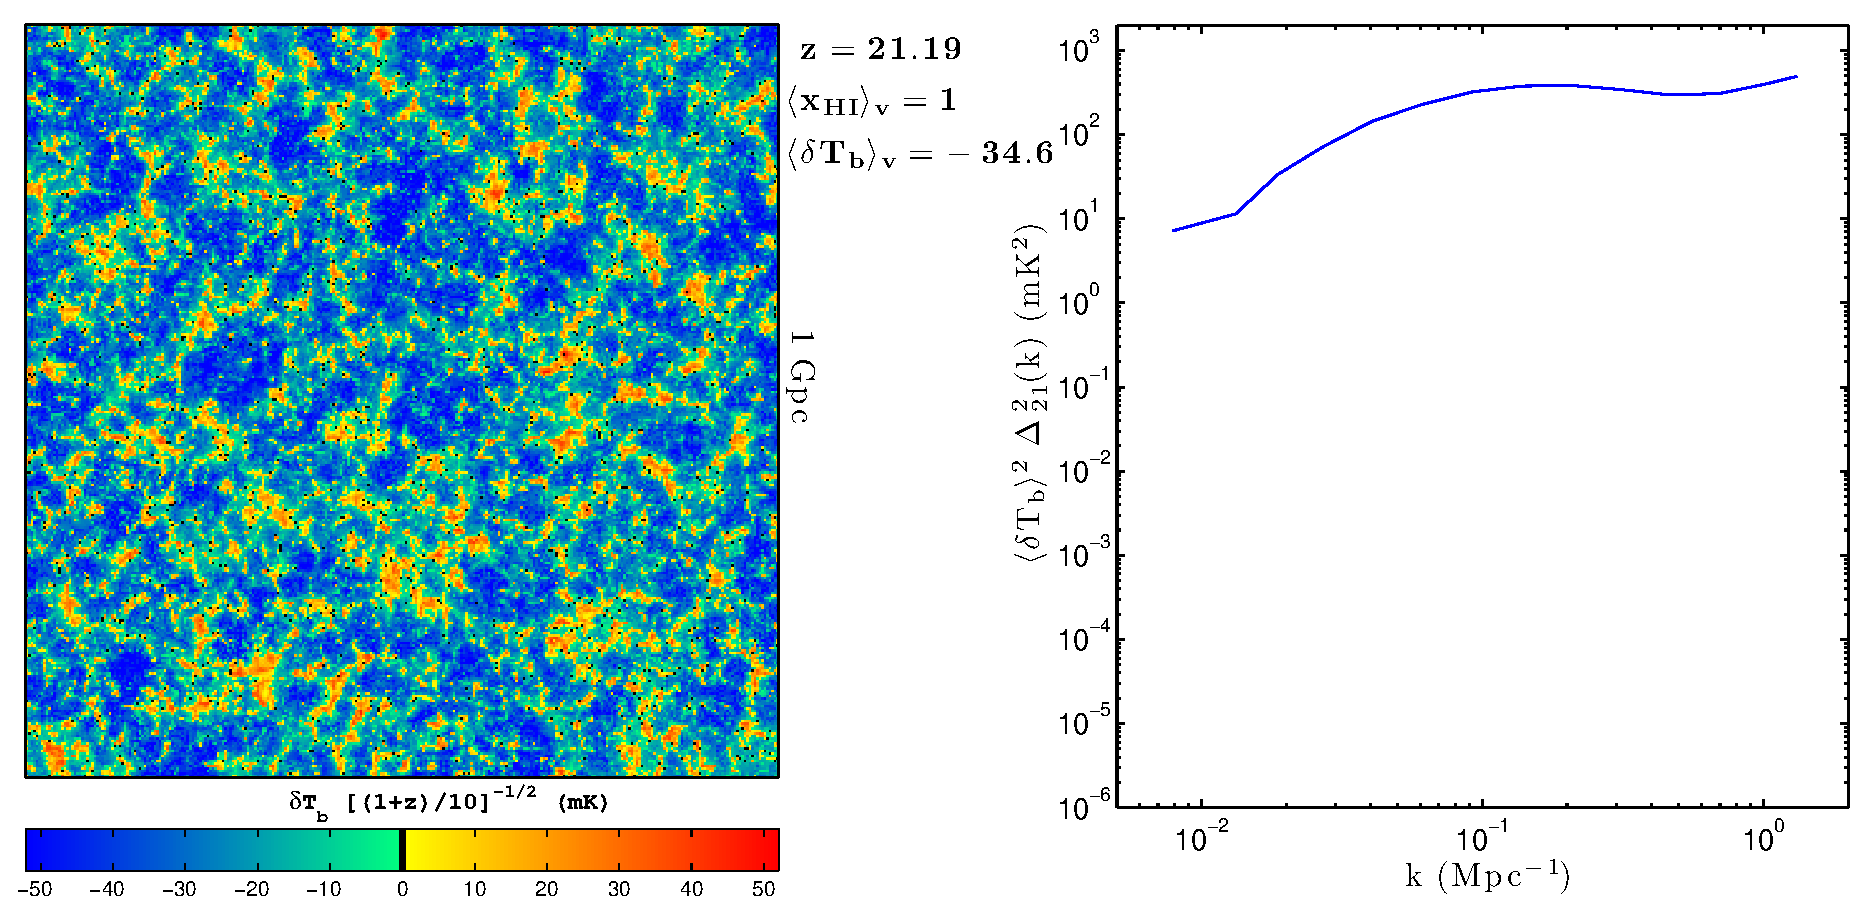
\includegraphics[width=125mm]{EoR/c03/c03.s1.f3b.eps}
\caption{$B%@!<%/%(%$%8!"(BCD$B$G$N(B$\delta T_{{\rm b}}$$B$N%^%C%W$H%Q%o!<%9%Z%/(B
 $B%H%k!J(BMesinger et al, 2010)$B!#:8$O(B$\delta T_{{\rm b}}$$B$N%^%C%W$G!"1&$,%Q(B
 $B%o!<%9%Z%/%H%k$N%0%i%U!#%Q%o!<%9%Z%/%H%k$N2#<4$OGH?t(B$k$$B$G=D<4$O%Q%o!<%9(B
 $B%Z%/%H%k!#%@!<%/%(%$%8=*HW$N(B$z$=30.07$B!"(BX$B@~$K$h$k2CG.$,==J,$K8z$/A0$N(B
 $z=21.19$$B$G$O!"51EY29EY$O(BCMB$B$KBP$9$k5[<}$H$7$F8+$($k!J(B$\delta T_{{\rm
 b}}<0$$B!K(B}
\label{fig:igm_history_darkage}
\end{figure}
%
\begin{figure}[htbp]
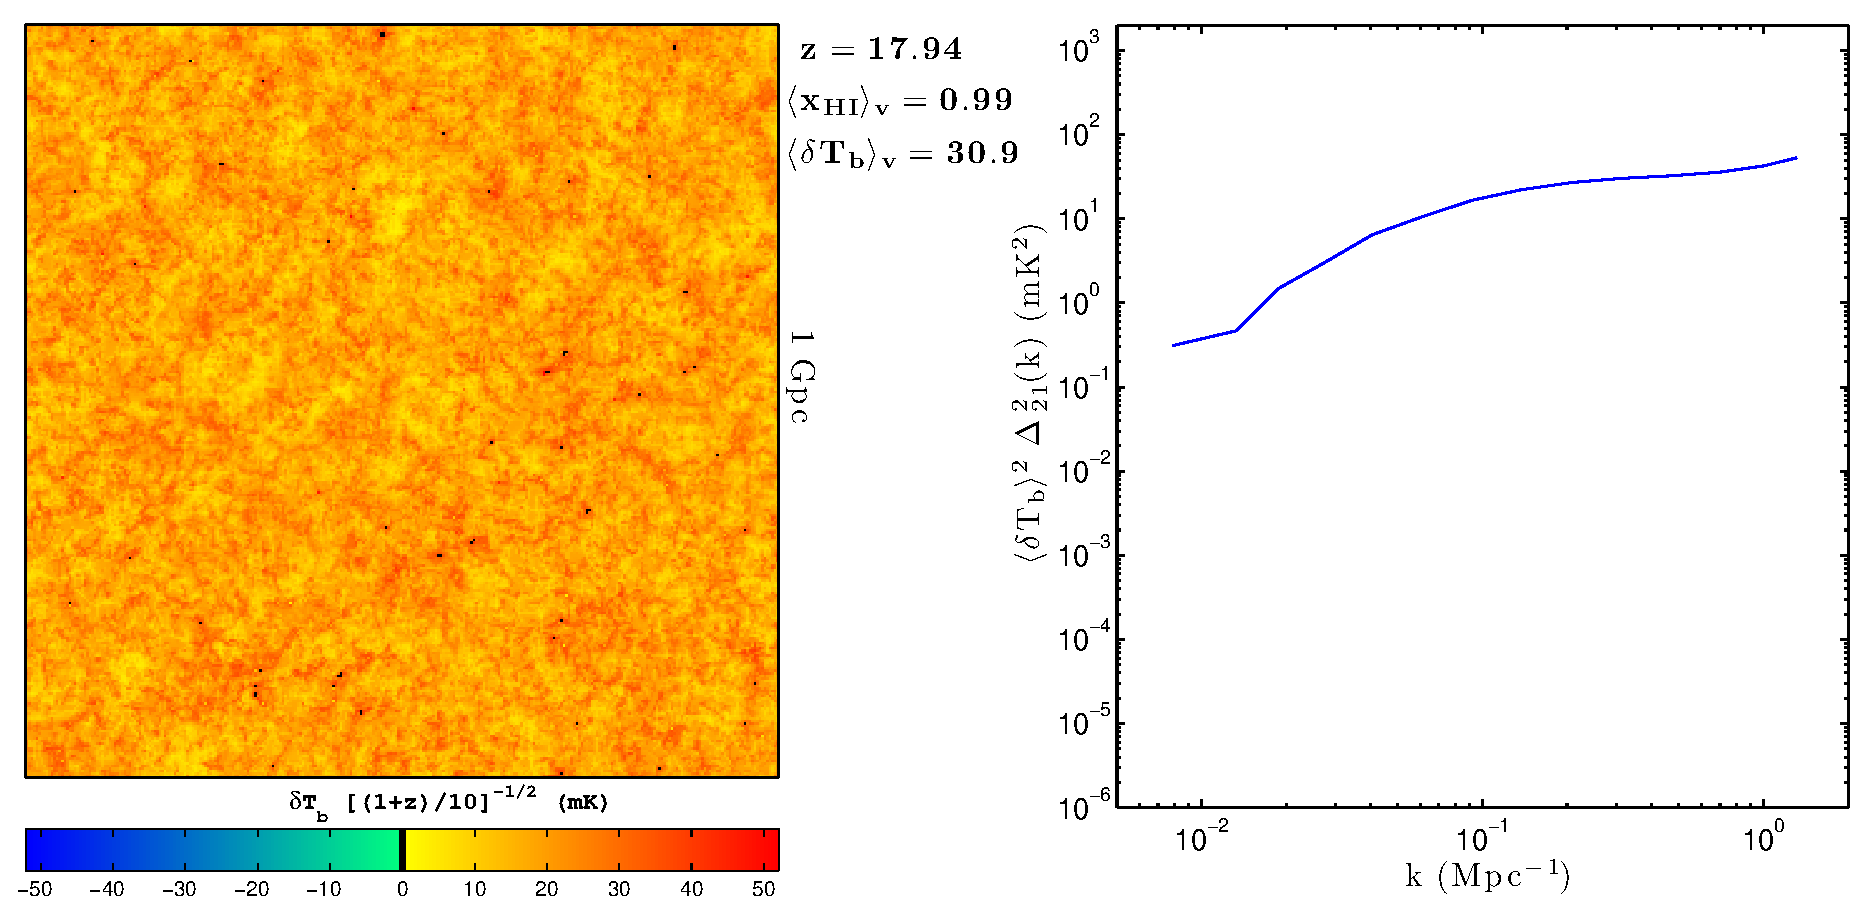
\includegraphics[width=125mm]{EoR/c03/c03.s1.f4a.eps}
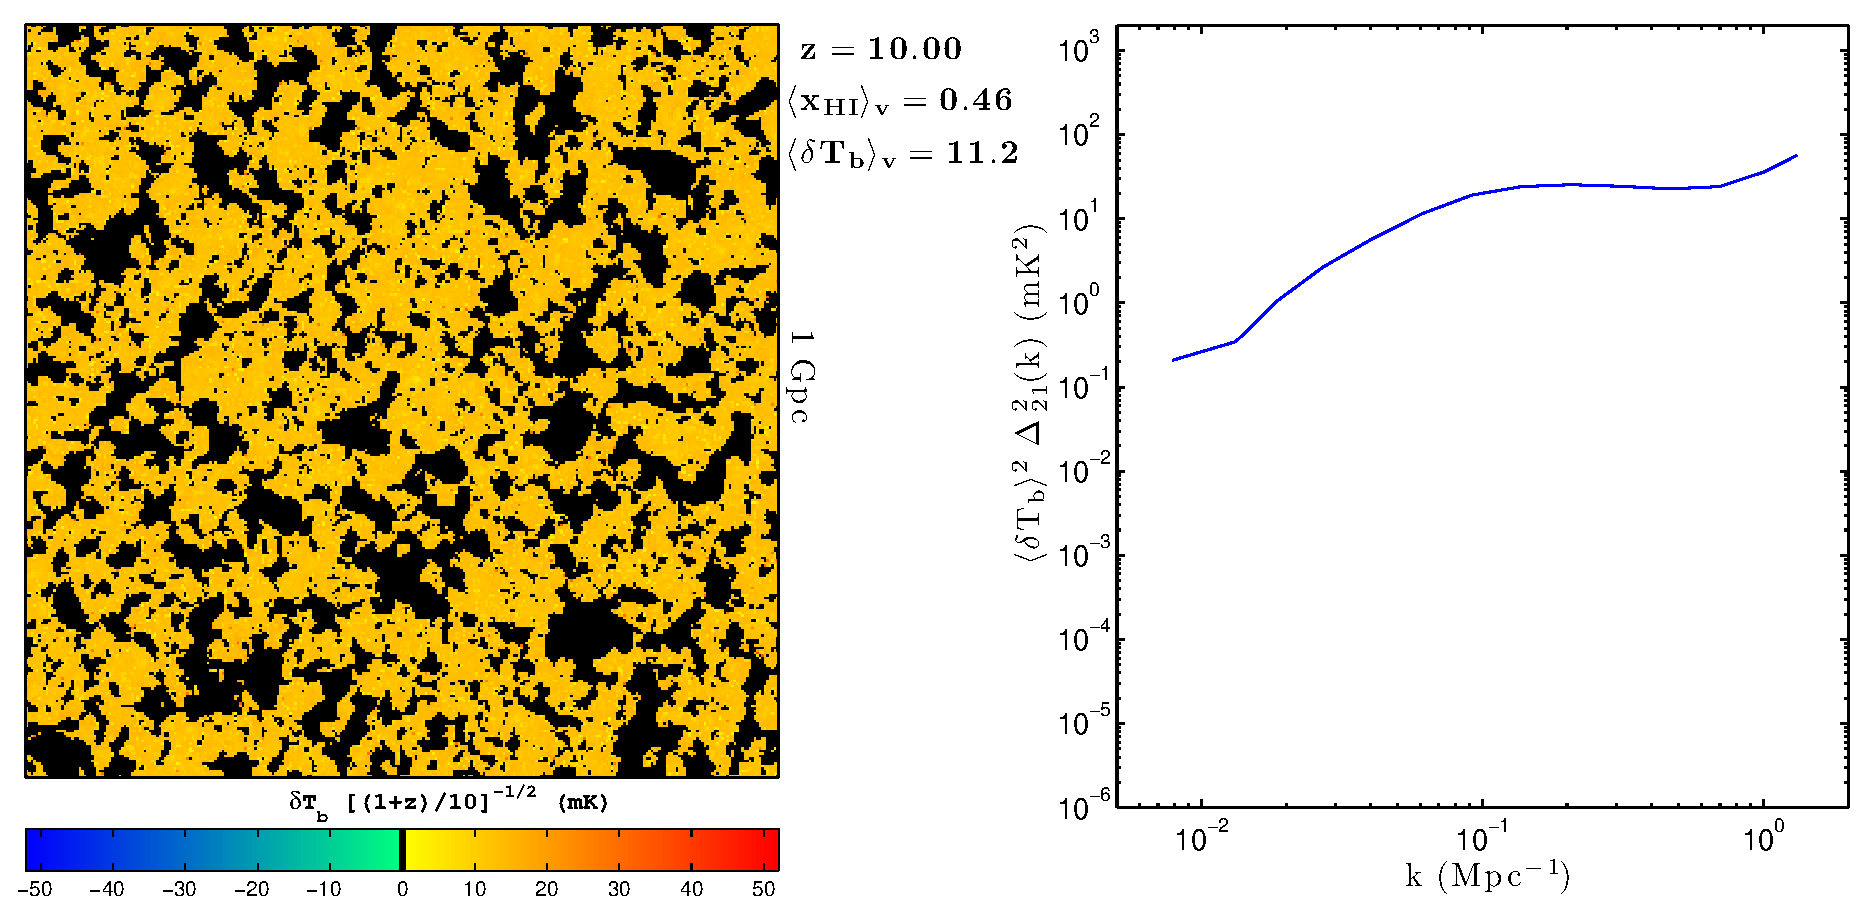
\includegraphics[width=125mm]{EoR/c03/c03.s1.f4b.eps}
\centering
\caption{$B:FEEN%4|$G$N(B$\delta T_{{\rm b}}$$B$N%^%C%W$H%Q%o!<%9%Z%/%H%k(B
 $B!J(BMesinger et al, 2010)$B!#2CG.$,==J,$K8z$$$F$$$k(B$z=17.94$$B$G$O!"51EY29EY(B
 $B$O51@~$H$7$F4QB,$5$l$k!J(B$\delta T_{{\rm b}}>0$$B!K!#$3$N$H$-!"?eAG$OCf@-(B
 $B>uBV$H$7$FB8:_$7$F$$$k$,!"(B$z=10.00$$B$K$J$k$H!":FEEN%$,;O$^$j!"?eAG$,%$%*(B
 $B%s2=$5$l$?NN0h$H!"Cf@->uBV$N$^$^$NNN0h$KJL$l$F$$$k$N$r8+$k;v$,$G$-$k!#(B
 $B%$%*%s2=NN0h$,%P%V%k$H$7$FI=$5$l!"Cf@->uBV$NItJ,$O%Q%C%A>u$K$J$C$F$*$j!"(B
 $BN><T$K$O6/$$%3%s%H%i%9%H$,$"$k!#(B}
\label{fig:igm_history_reionization}
\end{figure}

\subsubsection{$BB>$N4QB,NL(B}
$B%Q%o!<%9%Z%/%H%k0J30$K$b51EY29EY$+$iF@$i$l$k4QB,NL$H$7$F$O!"0J2<$N$b$N$,(B
$B5s$2$i$l$k!#(B
\begin{itemize}
\item $BJ,;6!"%b!<%a%s%H(B\\
      $B%Q%o!<%9%Z%/%H%k$,%U!<%j%(6u4V$GDj5A$5$l$kNL$G$"$k0lJ}$G!"<B6u4V>e$G$N51(B
      $BEY29EY>l$NE}7WE*@-<A$rC5$kJ}K!$H$7$F!"MI$i$.$NJ,;6$d9b<!$N%b!<%a%s(B
      $B%H(B($BODEY$d@mEY(B)$B$rMQ$$$kJ}K!$,$"$k!#EgB^$i$O%Q%o!<%9%Z%/%H%k$N;~4V0MB8@-$K(B
      $B$D$$$F!"51EY29EY$NJ,I[4X?t$NJ,;6$dODEY$KCmL\$7$F2r<a$rM?$($?(B
      \citep{Shimabukuro14}$B!#$3$l$K$h$k$H!"$I$N$h$&$JJ*M}%W%m%;%9$,(B
      $B%9%T%s29EY$r7h$a$F$$$k$+$K$h$C$FODEY$NId9f$,0[$J$j!"%Q%o!<%9%Z%/%H%k$N(B
      $B2r<a$r$9$k>e$GM-MQ$G$"$k!#(B
\item $B9b<!E}7WNL!"(B$n$$BE@Aj4X4X?t(B\\
      $B%U!<%j%(6u4V>e$N#2E@$r9M$($k$N$,%Q%o!<%9%Z%/%H%k$G$"$k0lJ}!"#3E@0J>e$r9M(B
      $B$($k9b<!E}7WNL$H$7$F!"%P%$%9%Z%/%H%k$,$"$k!#51EY29EY>l$NMI$i$.$,Hs(B
      $B%,%&%9J,I[$K=>$&>l9g!"%Q%o!<%9%Z%/%H%k$G$OC5$l$J$$>pJs$r%P%$%9%Z%/(B
      $B%H%k$O4^$s$G$$$k!#$^$?!"9b<!E}7WNL$r%U!<%j%(JQ49$7$F<B6u4V>e$G9M$((B
      $B$?$b$N$,(B$n$$BE@Aj4X4X?t$H$J$k!#5H1:$i$O(BSKA$B$d(Bpathfinder$B$N%P%$%9%Z%/%H%k$K(B
      $BBP$9$k46EY$r8+@Q$b$C$F$*$j!"(Bpathfinder$B$G$bBg%9%1!<%k(B
      $B!J(B$k \sim 0.1~{\rm Mpc^{-1}}$$B!K$G$"$l$P4QB,2DG=$G$"$k$3$H$r<($7$F$$$k!#(B
\item $B%H%b%0%i%U%#!<!"%$%a!<%8%s%0(B\\
      21cm$B@~$rMQ$$$?4QB,$G$O!"@VJ}JP0\Kh$N3,AXE*$J%^%C%W$N>pJs$r<j$KF~$l$k;v$,(B
      $B$G$-$k$N$G!"%H%b%0%i%U%#!<$r9M$($k;v$,$G$-$k!#$^$?!"%$%*%s2=%P%V%k(B
      $B$N?J2=$NMM;R$rC5$k<jK!$H$7$F!"51EY29EY$N6/EY$N6u4VE*J,I[$r4Q$k%$%a!<(B
      $B%8%s%0$,$"$k!#(B 
\item $B%$%*%s2=%P%V%k$dCf@-?eAGJ,I[$N%H%]%m%8!<(B\\
$B%$%*%s2=%P%V%k$dCf@-?eAGJ,I[$N4v2?3XE*$J>pJs$rC5$k<jK!$H$7$F!"%_%s%3%U%9(B
      $B%-!<HF4X?t$d%8!<%J%9E}7W$rMQ$$$kJ}K!$,$"$k!#(B 
\item $BGX7JEEGH8;$KBP$9$k(B21cm$B@~5[<}@~(B\\
      $BGX7JEEGH8;$+$iJ|<M$5$l$?EEGH$,(BIGM$B$d%_%K%O%m!<$K$h$k5[<}$r<u$1$k$H!"$=(B
      $B$NMM;R$O(B21cm$B@~$N5[<}@~$H$7$F4QB,$9$k;v$,$G$-$k!#(B 
\end{itemize}


\subsection{21cm$B@~%7%0%J%k$KBP$9$kA07JJ|<M(B}
$B$3$l$^$G8+$F$-$?$h$&$K!"(B21cm$B@~$O0E9u;~Be$+$i=iBeE7BN7A@.$r7P$F:FEEN%$^$G$N2aDx$rC5$k>e$G7hDjE*$K=EMW$JLr3d$r2L$?$9$H4|BT$5$l$k!#$7$+$7(B21cm$B@~%7%0%J%k$K$OB??t$=$7$F5pBg$JA07JJ|<M$,B8:_$7!"$3$l$r$J$s$i$+$NJ}K!$GHr$1$k$b$7$/$O:9$70z$+$J$1$l$P%7%0%J%k$rF@$k$3$H$O$G$-$J$$!#A07JJ|<M$O<g$K6d2O7OJ|<M$H7O30EEGHE7BN$N#2$D$KJ,$1$i$l!"0J2<$G6qBNE*$K@bL@$9$k!#(B

\paragraph{$B6d2O7OJ|<M(B}
$B6d2O7O$N%7%s%/%m%H%m%sJ|<M$H@)F0J|<M$O%7%0%J%k$KHf$Y$F05E]E*$KL@$k$/!"%Q%o!<%9%Z%/%H%k$K$*$$$F$O%7%0%J%k$N#67e0J>e$bBg$-$$!#$H$3$m$,N><T$H$b$K<~GH?t%9%Z%/%H%k$,Hs>o$K3j$i$+$G$"$k0lJ}!"%7%0%J%k$K$*$$$F$O%,%9L)EY$d%9%T%s29EY$N;k@~J}8~$K1h$C$?$f$i$.$rH?1G$7$F<~GH?t%9%Z%/%H%k$bBg$-$JJQF0$r;}$C$F$$$k$H4|BT$5$l$k!#$3$N$h$&$J@-<A$N0c$$$rMxMQ$7$F!"3F;k@~J}8~$KBP$7$F6d2O7OJ|<M$r8+@Q$b$C$F:9$70z$3$&$H$9$k;n$_$,9T$o$l$F$$$k!#<g$JJ}K!$H$7$F$O0J2<$N$h$&$JJ}K!$,5s$2$i$l$k(B\citep{Chapman15}$B!#(B
\begin{itemize}
\item $BB?9`<06a;w!'A07JJ|<M$N%9%Z%/%H%k$r<~GH?t$NDc<!$NB?9`<0$G$"$k$H2>Dj$7$F%U%#%C%H$7!"A07JJ|<M$r8+@Q$b$k!#$7$+$7<B:]$N%9%Z%/%H%k$,$I$N$h$&$J4X?t7A$K$J$C$F$$$k$+$o$+$i$:!"B?9`<0$N<!?t$r$$$/$D$K<h$k$+$K$h$C$F7k2L$,JQ$o$C$F$7$^$&$?$aG$0U@-$,$"$j!"8=:_$G$O$"$^$jM-MQ$JJ}K!$H$O9M$($i$l$F$$$J$$!#(B
\item Generalized Morphological Component Analysis$B!'A07JJ|<M$N%9%Z%/%H%k$,$"$k<o$N%7%s%W%k$5!J%9%Q!<%9@-!K$r;}$D$H$7$F?dDj$9$k!#6qBNE*$K$ONc$($P%9%Z%/%H%k$r%&%'!<%V%l%C%HJQ49$7$?;~$K$=$NE83+78?t$N$[$H$s$I$,%<%m$K$J$k$H2>Dj$9$k!#2r@O$KWs0U@-$,F~$i$J$$!#(B
\item Wp smoothing$B!'%9%Z%/%H%k$N6JN($NJQ2=$,$G$-$k$@$1>.$5$/$J$k$h$&$KA07JJ|<M$N4X?t7A$r8+@Q$b$k!#(B
\end{itemize}
$BB??t$NJ}K!$,Ds0F$5$l%7%_%e%l!<%7%g%s$,$5$l$F$$$k$,!"8=:_$N$H$3$m6d2O7OJ|<M=|5n$N7hDjBG$O$J$/!":#8e$NH/E8$,6/$/K>$^$l$F$$$k!#(B

\paragraph{$B7O30EEGHE7BN(B}
$B7O30$NEEGHE7BN$OE@8;$G$"$C$F$b43>D7WFCM-$N%S!<%`%Q%?!<%s$K$h$C$F<~0O$NNN0h$KO3$l=P$7$F$7$^$&!#$^$?;kLn$N9-$$K>1s6@$N>l9g$G$O!"Nc$(6d6KJ}8~$r4QB,$7$F$$$F$bBg$-$/9-$,$C$?%5%$%I%m!<%V$rDL$7$F6d2OLLJ|<M$,F~$j9~$s$G$/$k!#$3$l$i$rHr$1$k$?$a$K$OE75eLL>e$N$I$N0LCV$K$I$N$h$&$JL@$k$5$NE7BN$,B8:_$9$k$+$r5-=R$9$k%9%+%$%b%G%k$r@53N$K9=C[$7!"%S!<%`$N7A>u$b@53N$KM}2r$9$k$3$H$K$h$C$F4QB,%G!<%?$r3S@5$9$kI,MW$,$"$k!#$^$?CO5e$NEEN%7w$b%9%+%$%b%G%k$K1F6A$9$k$,!"EEN%7w$O;~!99o!9$HJQ2=$7!"$5$i$K43>D7W$N4p@~D9$,D9$$$H1F6A$r<u$1$kEEN%7w$N0LCV$,K>1s6@$4$H$K0[$J$k$?$a3S@5$O$h$j:$Fq$K$J$k!#(B

\paragraph{$B7W;;%3%9%H(B}
$BA07JJ|<M=|5n$N0lHLE*$J<jB3$-$H$7$F$O!"7O30$NEEGHE7BN$r3S@5$7$?8e!";k@~$4$H$K6d2O7OJ|<M$r=|5n$9$k$3$H$K$J$k!#@h$K=R$Y$?$h$&$KEEN%7w$O;~!99o!9$HJQ2=$9$k$?$a!"C;;~4V$N@QJ,$4$H$K3S@5$O9T$o$l$k!#$=$N$?$a3S@5$H6d2O7OJ|<M$N=|5n$K$OB?Bg$J7W;;%3%9%H$,$+$+$k$3$H$K$J$j!"$3$l$i$OC1$K@53N$J$@$1$G$J$/7W;;%3%9%H$b$*$5$($k$h$&$K$J$5$l$J$1$l$P$J$i$J$$!#$3$NE@$b:#8e$N2]Bj$G$"$k!#(B


\subsection{$B8=:_$N@)8B(B}
$B:FEEN%4|$KBP$9$k4QB,$O$3$l$^$G$K$b9T$o$l$F$*$j!"$=$l$K$h$C$F:FEEN%;K$d$=$l$K4XO"$9$k9b@VJ}JP0\$G$N@17A@.;K$KBP$9$k@)8B$,F@$i$l$F$$$k!#$3$N@a$G$O!"8=:_!":FEEN%4|$K$D$$$F4QB,E*$K$I$N$h$&$J@)8B$,$5$l$F$$$k$N$+=R$Y$k!#(B

$B$?$@$7!"8=:_F@$i$l$F$$$k$N$O:FEEN%4|=*N;4V:](B$(z\lesssim 10)$$B$N>pJs$@$1$G$"$j!":FEEN%3+;O;~4|$NJ*M}$O0MA3$H$7$FJ,$+$C$F$$$J$$$?$a!":#8e$N4QB,$NH/E8$,4|BT$5$l$k!#(B

\subsubsection{$B%,%s(B-$B%T!<%?!<%=%s$NC+(B}
$B9b@VJ}JP0\$G8+$D$+$C$?%/%(!<%5!<$N%9%Z%/%H%k$r8+$k$3$H$G!":FEEN%$N40N;$7(B
$B$?;~4|$r8+@Q$b$k$3$H$,$G$-$k!#1'Ch$KCf@-?eAG$,K~$A$F$$$k$H$-$O!"9b@VJ}JP(B
$B0\$N%/%(!<%5!<$+$iJ|<M$5$l$?%i%$%^%s(B$\alpha$$B8w;R$O!"Cf@-?eAG$K$h$C$F5[<}(B
$B$5$l$k!#$3$N$H$-!"2f!9$O!"1'ChKDD%$K$h$k@VJ}JP0\$K$h$C$F0z$-1d$P$5$l$?%i(B
$B%$%^%s(B$\alpha$$B8w;R$NGHD9$G!"5[<}@~%9%Z%/%H%k$r4QB,$9$k$3$H$,$G$-$k!#$^$?!"(B
$B%/%(!<%5!<$+$iJ|<M$5$l$?%i%$%^%s(B$\alpha$$B$h$j$bGHD9$NC;$$8w$O!"1'ChKDD%$K(B
$BH<$&@VJ}JP0\$N8z2L$K$h$C$F%i%$%^%s(B$\alpha$$B$NGHD9$K$J$j!"BP1~$9$k@VJ}JP0\(B
$B$NCf@-?eAG$K5[<}$5$l$k!#:FEEN%$,40N;$K6a$E$/$K$D$l!"Cf@-?eAG$,$J$/$J$k$?(B
$B$a!"5[<}@~%9%Z%/%H%k$,8+$($K$/$/$J$k!#$3$l$K$h$j!":FEEN%4|$N=*N;;~4|$r8+(B
$B@Q$b$k$3$H$,$G$-$k!#4QB,%9%Z%/%H%k$K9o$^$l$?5[<}@~$NO"$J$j$r%,%s(B-$B%T!<%?!<(B
$B%=%s$NC+$H8F$V!#$3$NJ}K!$K$h$C$F!"(B$z\sim6$$B$G:FEEN%$,=*N;$7$?;v$,$o$+$C$F(B
$B$$$k(B \citep{2006AJ....132..117F,2011Natur.474..616M}$B!#(B

\subsubsection{CMB$B;6Mp$N8w3XE*8|$_(B}
CMB$B8w;R$H:FEEN%4|$N%$%*%s2=%P%V%kCf$NEE;R$H$N;6Mp$K$h$C$F!"(BCMB$B$N%Q%o!<%9(B
$B%Z%/%H%k$KJP8w$K$h$k$f$i$.$,2C$o$j!"%9%Z%/%H%k$,JQ2=$9$k!#$=$3$+$i:FEEN%(B
$B$N4|4V$d%$%*%s2=N($NMI$i$.$J$I$K@)8B$rF@$k$3$H$,$G$-$k!#8=:_!"(BCMB$B$N;6Mp(B
$B$O(B$z\sim10$$B$G5/$3$j!"$=$N$H$-;6Mp$N8w3XE*8|$_$,(B$\tau\sim0.09$$BDxEY$G$"$k(B
$B;v$,J,$+$C$F$$$k(B \citep{2013arXiv1303.5081P}$B!#(B

\subsubsection{IGM$B29EY(B}
$z\approx 6$$B$N%/%(!<%5!<$N<~0O$N%,%929EY$r%U%)!<%/%H%W%m%U%!%$%kJ,@O(B($BJ,I[(B
$B$r%U%)!<%/%H4X?t$G%U%#%C%F%#%s%0(B)$B$K$h$C$FB,$j!"$=$l$H:FEEN%4|$G$N%/%(!<%5!<(B
$B<~JU$N@:L)$J%7%_%e%l!<%7%g%s$rHf3S$9$k$3$H$G!":FEEN%4|$N%,%929EY?J2=;K$K(B
$B@)8B$r2C$($k$3$H$,$G$-$k!#$3$l$K$h$l$P!"(BH\textsc{i}$B$NEEN%$O!"(B$z\lesssim
11$$B$G5/$3$C$?$H4|BT$5$l$k(B \citep{2010MNRAS.406..612B}$B!#(B

\subsubsection{$B%,%s%^@~%P!<%9%H(B}
$B%,%s%^@~%P!<%9%H(B(GRBs)$B$OBg<ANL@1$ND6?7@1GzH/$HL)@\$K4X78$7$F$$$k$H9M$($i(B
$B$l$F$$$k!#$7$?$,$C$F!"9b@VJ}JP0\$G(BGRBs$B$,4QB,$5$l$F$$$k;v<B$O!"1'Ch$N=i4|(B
$B$KBg<ANL@1$,B8:_$7$?2DG=@-$r<($7$F$$$k!#$3$l$K$h$j!":#8e$h$jB?$/$N9b@VJ}(B
$BJP0\(BGRBs$B$,4QB,$5$l$l$P!":FEEN%4|0JA0$NBg<ANL@1$N@17A@.N($K@)8B$r2C$($k$3(B
$B$H$,$G$-$k(B \citep{2009Natur.461.1254T}$B!#$^$?!"9b@VJ}JP0\(B GRBs$B$N0lIt$O%i(B
$B%$%^%s(B$\alpha$$B8:?jMc$N%U%#%C%F%#%s%0$K$h$k:FEEN%4|$NCf@-?eAG3d9g$N@)8B$K(B
$B$bMQ$$$i$l$F$$$k(B (e.g.,\cite{2006PASJ...58..485T}$B!#(B


\subsubsection{$B9b@VJ}JT0\6d2O(B}
$B9b@VJ}JT0\$G$NCf@-?eAG$K$h$k6/$$5[<}$r<u$1!"4QB,$5$l$F$$$J$$%I%m%C%W%"%&(B
$B%H6d2O$N4QB,$+$i!"@17A@.;K$K@)8B$r2C$($k$3$H$,$G$-$k!#8=:_$N4QB,$+$i$O!"(B
$z>10$$B$G5^7c$K@17A@.N($,2<$,$C$F$$$k;v$,<(:6$5$l$F$$$k(B
(\citep{2013ApJ...773...75O})$B!#$^$?!"(B$z>6$$B$N%i%$%^%s(B$\alpha$$B51@~6d2O$N8D(B
$B?tL)EY$O!"9b@VJ}JT0\$[$I>.$5$/$J$C$F$*$j!"$3$l$OCf@-?eAG$K$h$k8:8w$K5/0x(B
$B$9$k$H$b9M$($i$l$F$$$k(B (e.g.,\cite{2010ApJ...723..869O})$B!#(B


\subsubsection{$B6a@V30@~(B}
$B1'Ch=i4|$N6d2O$d@1$+$iJ|<M$5$l$?(BUV$B$O;d$?$A$,4QB,$9$k$^$G$K!"6a@V30$N<~GH(B
$B?t$^$G@VJ}JP0\$9$k!#$=$N6/EY$dHsEyJ}@-$+$i!"1'Ch=i4|$G$N;g30@~8;$NJ,I[$d(B
$BB8:_NLEy$N@-<A$K@)8B$,IU$1$i$l$k2DG=@-$,$"$k!#%Q%o!<%9%Z%/%H%k$KBP$9$k>e(B
$B8B$O$"$k$b$N$N!"M}O@CM$rBgI}$K>e2s$C$F$$$k(B \citep{2012ApJ...756...92C}$B!#(B
\subsubsection{X$B@~(B}
$BFp(BX$B@~(B(Soft X-ray)$BGX7JJ|<M6/EY$r4QB,$9$k$3$H$G!"?eAG86;R(B1$B8D$"$?$j$N(BX$B@~8w(B
$B;R?t$K@)8B$r2C$($k$3$H$,$G$-$k!#$5$i$K$=$3$+$i!"(BX$B@~$N%=!<%9$r@)8B$G$-$k!#(B
$BNc$($P(B$z=10$$BIU6a$N4QB,E*@)8B$K$h$k$H!"Bg<ANL(BX$B@~O"@1$H%@!<%/%^%?!<BP>CLG(B
$B$K$h$k?eAG86;R$"$?$j$N8w;R?t$O(B0.1$BDxEY$7$+L5$$$3$H$,$o$+$C$F$$$k!#$^$?!"(B
$B3hF06d2O3K(B(AGN)$B$O:FEEN%$K:GBg(B10\%$BDxEY$7$+4sM?$G$-$J$$$3$H$bJ,$+$C$F$$$k(B 
\citep{2012MNRAS.426.1349M}$B!#(B 



\subsubsection{SKA$B%Q%9%U%!%$%s%@!<(B}
SKA$B$N40@.$O$^$@$^$@1s$$$,!"8=:_(BSKA$B40@.$^$G$N;n83$d4QB,E*<B83$H$7$F$$$/$D(B
$B$+K>1s6@$,7z@_$5$l!"4QB,$,9T$o$l$F$$$k!#$=$l$i$N4QB,$+$i$b:FEEN%4|$N(B21cm
$B%Q%o!<%9%Z%/%H%k$KBP$9$k@)8B$,F@$i$l$F$$$k!#$3$3$G$O!"3FK>1s6@$H4QB,7k2L(B
$B$K$D$$$F4JC1$K?($l$k!#(B 

\subsubsection{GMRT}
GMRT(Giant Metrewave Radio Telescope)$B$O%$%s%I$K$"$k!#J,2rG=$O(B20$BIC3Q!":G(B
$B$bDc$$<~GH?tBS$,(B139.3$\sim$156.0MHz$B$r%+%P!<$7$F$*$j!"(B$z=8.1\sim9.2$$B$r8+(B
$B$k$3$H$,$G$-$k!#(B$z\sim8.8$$BIU6a$N%Q%o!<%9%Z%/%H%k$K$D$$$F$N>e8B$,F@$i$l$F(B
$B$$$k(B \citep{2013MNRAS.433..639P}$B!#(B

\subsubsection{MWA}
MWA(Murchison Widefield Array)$B%*!<%9%H%i%j%"$K@_CV$5$l$F$$$k!#(B128$B8D$N%"(B
$B%s%F%J$+$i@.$C$F$$$k!#(B2$BJ,3Q$NJ,2rG=$r;}$A!"<~GH?t(B80$\sim$300MHz$B$r4QB,2D(B
$BG=$G$"$k!#(Bz=9.5$B$NGH?t(Bk=0.046$\rm Mpc^{-1}$$B$G%Q%o!<%9%Z%/%H%k$NJ?J}:,$,(B
0.3K$B$h$j>.$5$$$H$$$&@)8B$rF@$F$$$k(B \citep{2014PhRvD..89b3002D})$B!#(B

\subsubsection{PAPER}
PAPER(Precision Array for Probing the Epoch of Reionization)$B$OFn%"%U%j%+(B
$B$K@_CV$5$l$F$$$k!#(B32$B$N%"%s%F%J$+$i@.$C$F$$$k!#%Q%o!<%9%Z%/%H%k$KBP$7$F!"(B
z=7.7$B$G(Bk=0.11h$\rm Mpc^{-1}$$B$G>e8B(B2704$\rm mK^{2}$$B$rM?$($k(B \citep{2014ApJ...788..106P}$B!#(B
\subsubsection{LOFAR}
LOFAR(LOw Frequency ARray)$B$O%*%i%s%@KLIt$rCf?4$H$7$F!"9-0h$K%"%s%F%J$rG[(B
$BCV$7$F!"$=$l$i$r0l$D$NEEGH43>D7W$H$7$F07$&!#$=$ND>7B$O(B100km$B$K$b$N$\$j!"(B
$B<~GH?t$O(B10$\sim$250MHz$B$,4QB,2DG=$G$"$k(B\citep{2013A&A...556A...2V}$B!#(B



%未解決のサイエンス


%\setcounter{section}{2}
\section{国際SKAのサイエンス}\label{c03.s2}
\subsection{$B:FEEN%$NJ*M}(B}\label{c03.s2.ss1}%\label{phys}
\subsubsection{$BF3F~(B}

$B3F>l=j$G$NEEN%EY(B$x_{\rm \textsc{Hii}}$$B$N?J2=$O0J2<$N$h$&$KI=$;$k!#(B
\begin{equation}
\frac{d x_{\rm \textsc{Hii}}}{dt} = k_{\rm col} (T) (1-x_{\rm
 \textsc{Hii}})n_{\rm e} - \alpha(T)x_{\rm \textsc{Hii}} n_{\rm e} +
 k_{\rm ph}(1-x_{\rm \textsc{Hii}}) 
\end{equation}
$B$3$3$G!"(B$k_{\rm col}(T)$$B$O>WFMEEN%N(!"(B$n_{\rm e}$$B$OEE;R?tL)EY!"(B
$\alpha(T)$$B$O:F7k9gN(!"(B$k_{\rm ph}$$B$O8wEEN%N($G$"$k!#8wEEN%N($O!"3FCOE@$G(B
$B$NmU<M6/EY(B$I_\nu$$B$rMQ$$$F!"(B
\begin{equation}
k_{\rm ph}= \int d\Omega \int_{\nu_{\rm L}}^\infty
 \frac{I_\nu}{h\nu}\sigma_\nu d\nu 
\end{equation}
$B$HI=$;$k!#$3$3$G!"(B$\nu_{\rm L}$$B$O%i%$%^%sC<?6F0?t!"(B$\sigma_\nu$$B$OEEN%CGLL(B
$B@Q$G$"$k!#8wEEN%2aDx$O!"%(%M%k%.!<J}Dx<0$H$b%+%C%W%k$9$k0Y!"EEN%?J2=$HF1(B
$B;~$K%(%M%k%.!<J}Dx<0(B
\begin{equation}
\frac{du}{dt} = \frac{\Gamma - \Lambda}{\rho}
\end{equation}
$B$r2r$/I,MW$,$"$k!#$3$3$G!"(B$u$$B$OC10L<ANL$"$?$j$NFbIt%(%M%k%.!<$G$"$k!#$^(B
$B$?!"(B$\Gamma$$B$OC10LBN@Q$"$?$j$N2CG.N(!"(B$\Lambda$$B$OC10LBN@Q$"$?$jNd5QN($G(B
$B$"$j!"$3$l$i$K$O!"8w2CG.!"CGG.2CG.(B($BNd5Q(B)$B!">WFMEEN%Nd5Q!":F7k9gNd5Q!">WFM(B
$BNe5/Nd5Q!"@)F0J|<MNd5Q!"%3%s%W%H%s2CG.(B($BNd5Q(B)$B$J$I$,4^$^$l$k!#FC$K8w2CG.N((B
$B$O!"(B
\begin{equation}
\Gamma_{\rm ph}= n_{\rm \textsc{Hi}}\int d\Omega \int_{\nu_{\rm L}}^\infty \frac{I_\nu}{h\nu}(h\nu-h\nu_{\rm L})\sigma_\nu d\nu
\end{equation}
$B$HI=$;$k!#(B
$BEEN%$5$l$?%,%9$O!"$*$h$=(B10,000-20,000K$B$^$G2CG.$5$l$k(B(e.g.,
\cite{1996ApJ...465..608T})$B!#$3$N2CG.$K$h$j!"=ENO%]%F%s%7%c%k$N@u$$%,%9(B
$B1@$N=ENO<}=L$OAK32$5$l!"9b$$%,%905$K$h$C$F>.$5$J%9%1!<%k$N9=B$$O6Q$5$l$k!#(B
$B$3$N2aDx$r8w>xH/(B(photo-evaporation)$B$H8F$V!#(B

\subsubsection{$BEEN%2aDx$X$NF6;!(B}
\noindent\underline{\bf $BJ?6Q<+M39TDx(B}$B!!1'Ch$G$NEEN%8w;R$NJ?6Q<+M39TDx$O!"(B
\begin{equation}
l = \frac{1}{\sigma_\nu n_{\rm \textsc{Hi}}}\approx 2 \left(\frac{10}{1+z}\right)^2\left(\frac{\nu}{\nu_{\rm L}}\right)^3 \left(\frac{1}{x_{\rm \textsc{Hi}}}\right)\;{\rm comoving\;kpc}
\end{equation}
$BDxEY$G$"$k!#EEN%GHLL$N8|$5$OJ?6Q<+M39TDxDxEY$H$J$k$H9M$($i$l!";g30@~$N>l9g!"J?6Q<+M39TDx$O>.$5$$$?$a!"EEN%GHLL$OHs>o$K%7%c!<%W$K$J$k!#(B
$B0lJ}$G!"(B1keV$B0J>e$N(BX$B@~$NJ?6Q<+M39TDx$O(B$\sim$1 comoving  Gpc$B$H$J$j!"DcEEN%(B
$BEY$+$D0lMM$K6a$$EEN%9=B$$,4|BT$5$l$k!#(B

\noindent\underline{\bf $B:F7k9g;~4V(B}$B!!EEN%%,%9$O!"$*$h$=(B$T=10^4$K$B$KJ]$?$l(B
$B$k!#$3$N$H$-$N:F7k9gN($rMQ$$$F!"1'Ch$NJ?6QL)EY$G$N:F7k9g;~4V$O!"(B 
\begin{equation}
t_{\rm rec} = \frac{1}{\alpha (T)n_{\rm H}}\approx 240 \left(\frac{10}{1+z}\right)^3 {\rm Myr}
\end{equation}
$B$H$J$k!#9b@VJ}JP0\(B($1+z>10$)$B$K$*$$$F!"%_%K%O%m!<$d%U%#%i%a%s%H$J$I$N9=B$(B
($\frac{\delta \rho}{\rho}>20 $)$B$G$O!":F7k9g;~4V$O$*$h$=(B10Myr$B0J2<$H$J$j!"(B
$B$3$N$h$&$J9=B$$O!"8w>xH/$K$h$C$F9=B$$,$J$i$5$l$k$^$G8w;R5[<}BN$H$7$FF/$/(B
\citep{2014MNRAS.440.1662S}$B!#(B 

\noindent\underline{\bf $BM}A[%9%H%m%`%0%l%s5e(B}$B!!0lMML)EY>l$N>l9g!"8w;R8;(B
$B<~$j$NEEN%NN0h$O%9%H%m%`%0%l%s5e$H8F$P$l$k%b%G%k$GI=$;$k!#%9%H%m%`%0%l%s(B
$B5e$N%5%$%:(B($B%9%H%m%`%0%l%sH>7B(B)$B$O!"NN0hFb$G$NC10L;~4V$"$?$j$N:F7k9g?t$HEE(B
$BN%8w;R?t$,D`$j9g$$$K$h$C$F7hDj$5$l!"(B 
\begin{equation}
r_{\rm S} = \left( \frac{3 \dot{N_{i}}}{4\pi n_{\rm H}^2 \alpha_{\rm B} (T)}\right)^{\frac{1}{3}}
\end{equation}
$B$HI=$;$k!#$3$3$G!"(B$\dot N_{i}$$B$OEEN%8w;RJ|<MN(!"(B$\alpha_{\rm B}(T)$$B$OBh0lNe5/>u(B
$BBV0J>e$N=`0L$X$N:F7k9gN($G$"$k!#$3$N%b%G%k$rMQ$$$k$H!"Nc$($P(B$\dot N_{i}=5\times 10^{48}$/s, $n_{\rm H}=10^{-3}\rm cm^{-3}$$B$N$H$-(B$r_{\rm s}\approx
5.4$kpc$BDxEY$H$J$k!#(B

\subsubsection{$B86;O6d2OFb$K$*$$$F:FEEN%$K4XO"$9$k=t2aDx(B}
\noindent\underline{\bf $BEEN%8w;R$NC&=P(B}$B!!6d2O4VJ*<A$NEEN%?J2=$N2rL@$K$O!"(B
$B6d2O$+$iH4$1=P$9EEN%8w;R$NNL$,=EMW$H$J$k!#$3$NNL$O!"FC$K@17A@.N($HEEN%8w(B
$B;R$NC&=P3d9g(B($BC&=P8w;RN((B)$B$KJ,$1$F9M$($k$N$,JXMx$G$"$k!#:FEEN%4|$N8e4|CJ3,(B
$B$G$O!"6d2OFb$N%@%9%H$bC&=P8w;RN($K4X$7$F=EMW$JLr3d$r2L$?$92DG=@-$,$"$k!#(B 

$B4QB,E*$JC&=P8w;RN($r8+@Q$b$j$O!"6d2O4VJ*<A$N6/$$5[<}$K$h$jHs>o$K:$Fq$G$"(B
$B$k$,!"(B$z\approx3$$B$G$OD>@\E*$KEEN%8w;R$,8!=P$5$l$F$*$j!"?t%Q!<%;%s%H$+$i(B
$B?t(B10$B%Q!<%;%s%H$NCM$,<($5$l$F$$$k(B (e.g., \cite{2001ApJ...546..665S,
2009ApJ...692.1287I})$B!#$h$j9b@VJ}JP0\6d2O$K$D$$$F$O!"$$$/$D$+$N2>Dj$N4p(B
$B$E$-!"C&=P8w;RN($K>e8B(B($B@VJ}JP0\(B$z=5.7$$B$G(B$\sim60$$B%Q!<%;%s%H(B)$B$rM?$($?8&5f(B
$B$,$"$k(B (e.g.,\cite{2010ApJ...724.1524O})$B!#4QB,$5$l$k6d2O$N8D?tL)EY$+$i$O!"(B
$B@1$,:FEEN%$N<g$J8w;R8;$G$"$k>l9g!"9b@VJ}JP0\$[$I9b$$C&=P8w;RN(!"$"$k$$$O(B
$BDc<ANL6d2O$[$I9b$$C&=P8w;RN($G$J$$$H%H%`%=%s;6Mp$N8w3XE*8|$_$N4QB,7k2L$r(B
$BK~$9$3$H$,:$Fq$G$"$k$H<(:6$5$l$k(B (e.g., \cite{2012ApJ...759L..38A,
2012ApJ...746..125H, 2012MNRAS.419.1480M})$B!#(B 

$BM}O@E*$K$O!"<g$K?tCM%7%_%e%l!<%7%g%s$K$h$C$FC&=P8w;RN($,D4$Y$i$l$F$$$k(B
(e.g., \cite{2008ApJ...672..765G, 2009ApJ...693..984W,
2010ApJ...710.1239R, 2011MNRAS.412..411Y, 2013MNRAS.429L..94P,
2014MNRAS.442.2560W})$B!#$3$l$i$N7W;;7k2L$O!"J,2rG=$N0c$$!"%b%G%k$N0c$$$J(B
$B$I$+$iDjNLE*$K$OCM$,<}B+$7$F$$$J$$$,!"C&=P8w;RN($NDj@-E*$J?6$kIq$$$H$7$F(B
1) $B%O%m!<<ANL$,Bg$-$$$[$I>.$5$$!"(B2) $B9b@VJ}JP0\$[$IBg$-$$!"$H$$$&7k2L$,B?(B
$B$$!#(B 

\noindent\underline{\bf $B86;O6d2O$G$NmU<M@-%U%#!<%I%P%C%/(B}$B!!8w2CG.$dmU<M(B
$B05$H$$$C$?%U%#!<%I%P%C%/$O!"6d2OFb$N%,%9$d6d2O$X9_Ce$9$k%,%9!"6d2O4V%,%9(B
$B$N%@%$%J%_%/%9$K1F6A$rM?$($k(B (e.g., \cite{2009MNRAS.400.1283I,
2012MNRAS.427..311W, 2012MNRAS.424..377D, 2013MNRAS.428..154H}) $B!#(B
$B$3$N8z2L$O!"@17A@.N($N$_$J$i$:>e5-$NC&=P8w;RN($K$b1F6A$rM?$((B
$B$k;v$,<($5$l$F$$$k(B (e.g., \cite{2009ApJ...693..984W,
2012PTEP.2012aA306U})$B!#$^$??eAGJ,;R$N2rN%8w;R$O!"1'Ch=i4|$N<g$?$kNd5Q:`(B
$B$G$"$k?eAGJ,;R$r2rN%$9$k$?$a!"$3$N2aDx$b@17A@.N($K1F6A$rM?$($k!#$3$l$i(B
$BmU<M@-%U%#!<%I%P%C%/$rE,@Z$K9MN8$9$k;v$O!"6d2O$+$i$NEEN%8w;R6!5kNL$rL@$i(B
$B$+$K$9>e$GHs>o$K=EMW$G$"$k!#(B 

\subsubsection{$B6d2O4VJ*<A$G$NEEN%2aDx(B}
\noindent\underline{\bf $BEEN%GHLL$NH/E8(B}$B!!(B
$B0lMM$+$DDj>o$JL)EY>l$N>l9g!"EEN%GHLL$NH/E8$O!"EEN%GHLL$G$NEEN%8w;R%U%i%C(B
$B%/%9$HEEN%%,%9%U%i%C%/%9$ND`$j9g$$$+$i!"%9%H%m%`%0%l%sH>7B(B$r_{\rm S}$$B!"(B
$B:F7k9g;~4V(B$t_{\rm rec}$$B$rMQ$$$F(B
\begin{equation}
r_{\rm I} = r_{\rm S}[1- \exp(-t/t_{\rm rec})]^{\frac{1}{3}}
\end{equation}
$B$HI=$;$k(B \citep{Spitzer78} $B!#$b$7!"9bL)EY%,%92t$,B8:_$9$k>l9g!"$3$N%,%9(B
$B2t$,8w>xH/$5$l$J$$8B$j!"EEN%GHLL$O%,%92tFb$KJa$o$l$k(B ($B?^(B\ref{KH1})$B!#(B\\

\underline{{\bf X$B@~$K$h$kEEN%$H2CG.(B}}$B!!(BX$B@~$OM-8z$JEEN%8w;R8;$G$"$k$,!";g(B
$B30@~$H$O0[$J$j(BX-ray$B$OJ?6Q<+M39TDx$,Bg$-$$0Y!"1'ChKDD%$K$h$k?6F0?t$NJQ2=(B
$B$r9MN8$9$kI,MW$,$"$k!#$^$?!"8D!9$N8w;R$,$b$D%(%M%k%.!<$,9b$$0Y!"EEN%$N:](B
$B$KHt$S=P$9EE;R$K$h$kFs<!E*$J>WFMEEN%(B(secondary ionization)$B$N8z2L$b9MN8$9(B
$B$kI,MW$,$"$k(B (e.g.,\cite{2010A&A...523A...4B})$B!#(B 

%figure moved to ss2
%再電離の物理
\subsection{$B:FEEN%4|$N%b%G%j%s%0$H(BSKA$B$X8~$1$?%7%_%e%l!<%7%g%s(B}\label{c03.s2.ss2}%\label{EoRSim}

\begin{figure}[!t]
	\centering
	{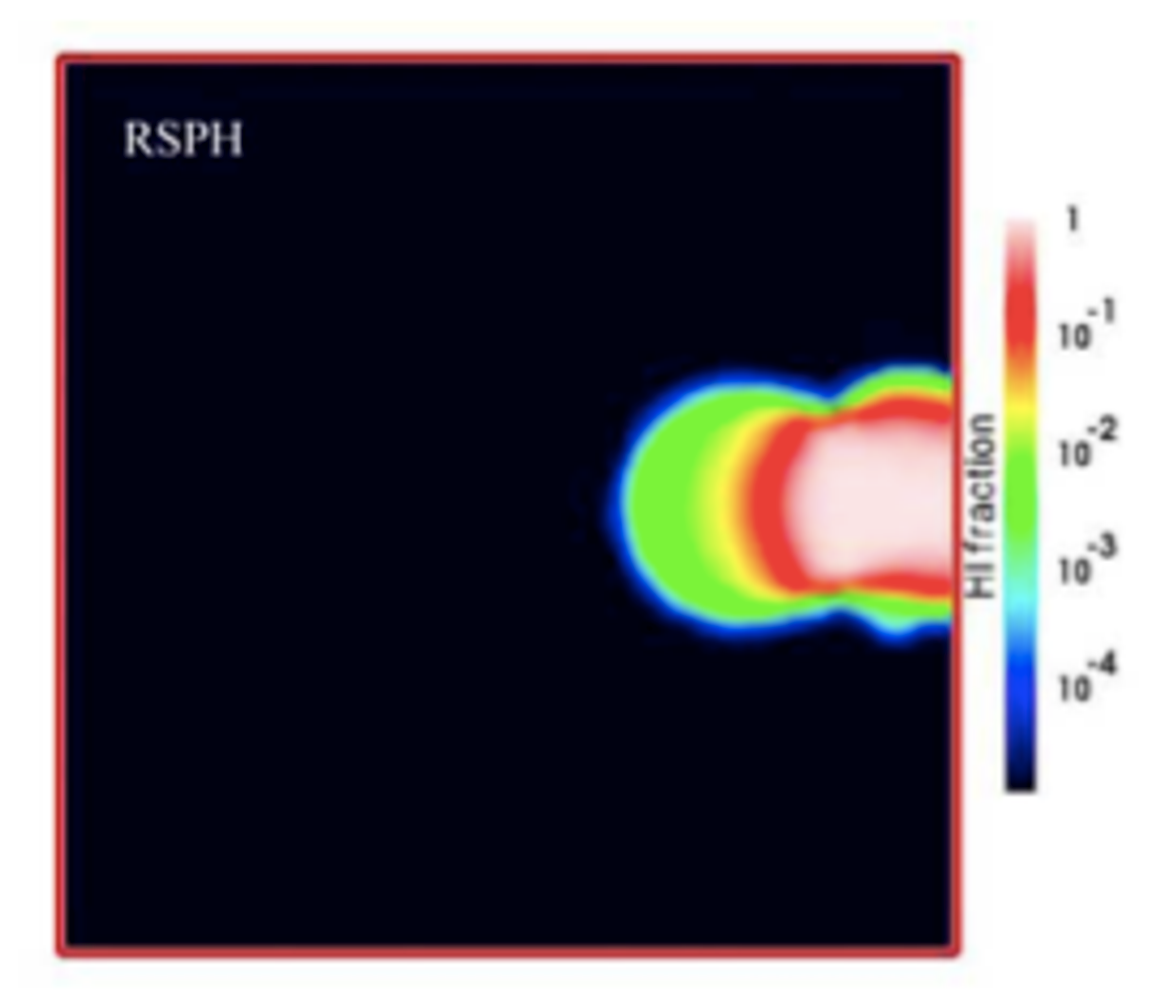
\includegraphics[width=7.5cm]{EoR/c03/c03.s2.f1a.eps}}
	{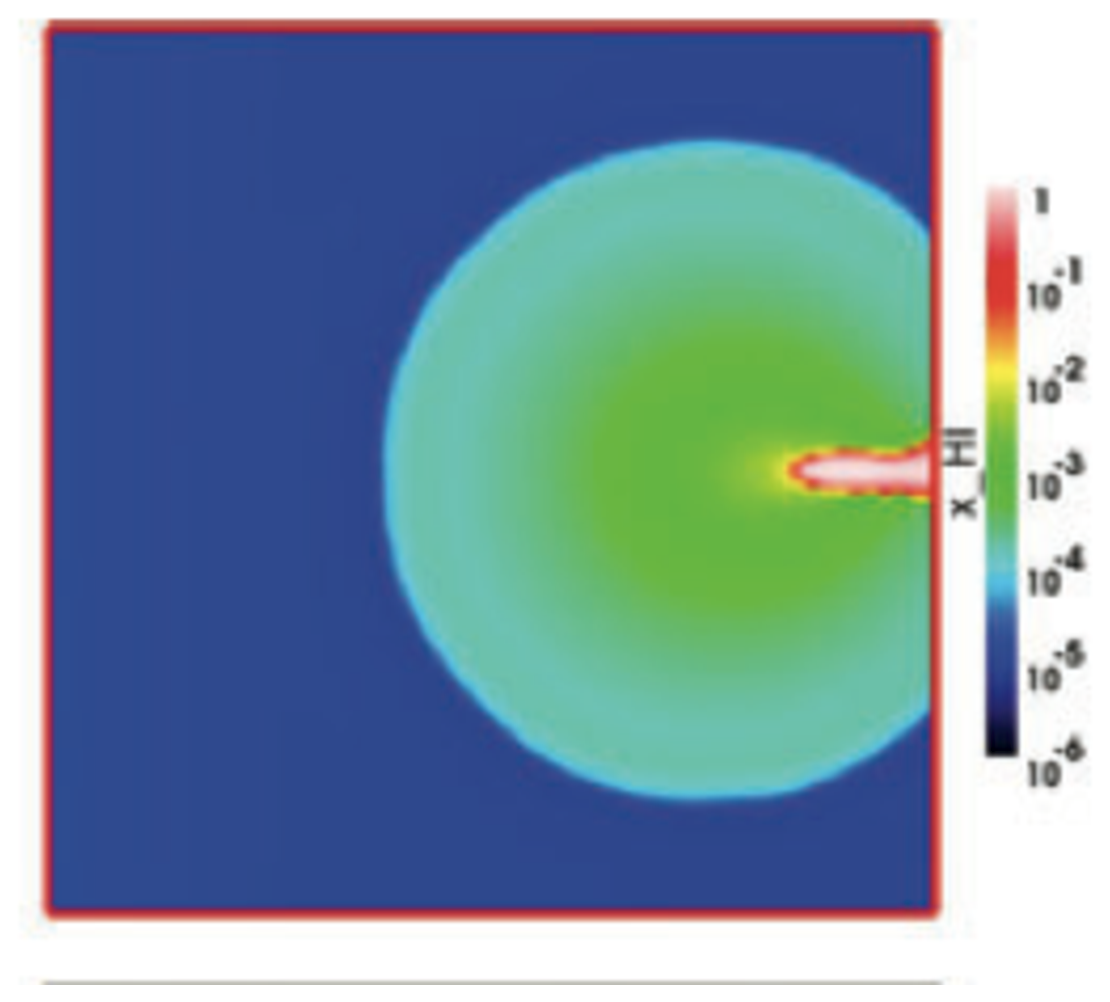
\includegraphics[width=7.5cm]{EoR/c03/c03.s2.f1b.eps}}
	\caption{$B:8$+$i0lMMEEN%8w;R%U%i%C%/%9$,9bL)EY%,%92t$KF~<M$9$k>l9g$N7W;;7k2L(B(\cite{2009MNRAS.400.1283I}, RSPH$BK!$K$h$k7W;;7k2L$rH4?h(B)$B!#:8?^!'@EE*$J%,%9$N>l9g!"EEN%GHLL$O%,%92t$KJa$o$l$k!#1&?^!'F0E*$J%,%9$N>l9g!"%,%92t$O8w>xH/$7!"EEN%GHLL$,?J$`$h$&$K$J$k!#(B}\label{KH1}
\end{figure}
\begin{figure}[!h]
	\centering {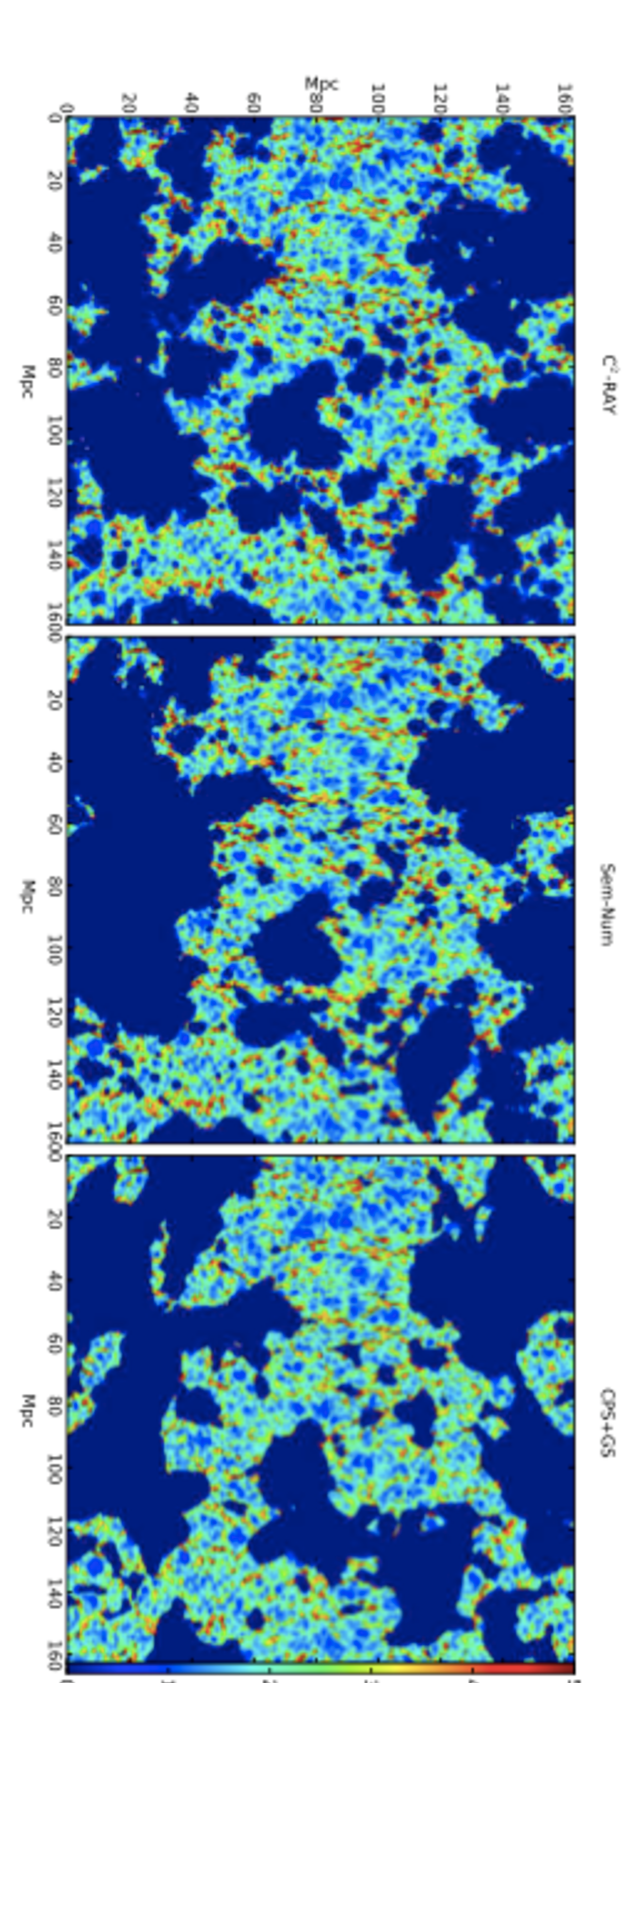
\includegraphics[width=0.3\linewidth,
	angle=90]{EoR/c03/c03.s2.f2.eps}} 
\caption{$BmU<MM"Aw%7%_%e%l!<%7%g%s(B($B:8?^(B)$B!"%O%m!<J,I[$rMQ$$$?=`?tCME*:FEEN%(B
	$B%7%_%e%l!<%7%g%s(B($BCf1{?^(B)$B!"(BPress-Schechter$B$rMQ$$$?=`?tCME*:FEEN%%7(B
	$B%_%e%l!<%7%g%s(B($B1&?^(B)$B$K$h$k(B21 cm$B@~6/EYJ,I[$NHf3S!#%O%m!<J,I[$rMQ$$$?(B
	$B=`?tCME*:FEEN%%7%_%e%l!<%7%g%s$G$O!"mU<MM"Aw%7%_%e%l!<%7%g%s$N(B21 cm
	$B@~6/EYJ,I[(B
	$B$r$h$/:F8=$G$-$k$,!"(BPress-Schechter$B$rMQ$$$?=`?tCME*:FEEN%%7(B
	$B%_%e%l!<%7%g%s$G$O!"mU<MM"Aw%7%_%e%l!<%7%g%s$N:F8=@-$OMn$A$k(B
	$B$3$H$,$o$+$k!#(B
	\citep{2014MNRAS.443.2843M}$B!#(B}\label{KH6}
\end{figure}
SKA$B$K$h$k@VJ}JP0\$7$?(B21 cm$B@~4QB,$G$O!":FEEN%4|$d$=$l0JA0$N;~4|$K$*$1$k(BIGM
$B$N(B3$B<!85%H%b%0%i%U%#!<$,F@$i$l$k$H4|BT$5$l$k!#<B:]$K4QB,$5$l$k$G$"$m$&(B
21 cm$B%7%0%J%k$O:FEEN%$NHs0lMM@-$K5/0x$9$k%Q%?!<%s$K4XO"$7$?Hs>o$KBg$-$J%9(B
$B%1!<%k$N$b$N$G$"$k$N$KBP$7!"2f!9$,CN$j$?$$$N$O!"=iBe6d2O$N$h$&$KHs>o$K>.(B
$B$5$/0E$$E7BN$N>pJs$G$"$k0Y!"$=$3$K$OBg$-$J3V$?$j$,B8:_$9$k!#=iBe6d2O$NFC(B
$BD'(B (Spectral Energy Distribution: SED$B!"8D?tEy(B) $B$N4QE@$+$i!"4QB,$5$l$k(B21
cm$B%7%0%J%k$r2r<a$9$k:]$K$O!"$3$l$i$N>\:Y$J%b%G%j%s%0$,=EMW$H$J$k!#(B 


$B6aG/$N:FEEN%%b%G%j%s%0$G$O!"<g$KD>@\E*$J?tCM%7%_%e%l!<%7%g%s$d=`2r@OE*(B/$B=`(B
$B?tCME*(B(semi-analytic/semi-numerical)$B%b%G%j%s%0(B
\citep{2004ApJ...613...1F, 2005ApJ...630...657Z, 2009ApJ...703L.167A,
2007ApJ...663..693M,2009MNRAS.394..960C,2010MNRAS.406..2421S}$B$,MQ$$$i$l$k!#(B



\subsubsection{$B8=B8$9$k%b%G%j%s%0$NMW;](B}
\noindent\underline{\bf $B%7%_%e%l!<%7%g%s(B}$B!!%7%_%e%l!<%7%g%s$O!"Bg$-$/(B2$B$D(B
$B$N%?%$%W$KJ,$1$i$l$k!#$R$H$D$O!">.7W;;NN0h$+$D9bJ,2rG=$N%7%_%e%l!<%7%g%s(B
$B$G$"$j!"$3$l$K$h$j6d2O7A@.$K$*$1$kmU<M$dD6?7@1GzH/$K$h$k%,%9$X$N%U%#!<%I%P%C%/(B
$B$r>\:Y$K8&5f$G$-$k$,!"Bg6IE*$J:FEEN%$d$=$N4QB,E*:/@W$rI=8=$9$k$N$K$O7W;;(B
$BNN0h$,IT==J,$G$"$k(B\citep{1997ApJ...486...581G,2000MNRAS.314..611C, 2002ApJ...575..33R}$B!#$b$&0l$D$O!"Bg$-$J7W;;NN0h$G$N(B
$B%7%_%e%l!<%7%g%s$G$"$j!">.%9%1!<%k$NJ*M}$OJ,2r$G$-$J$$JQ$o$j$K!"%0%m!<%P(B
$B%k$J:FEEN%?J2=$r8&5f$G$-$k(B\citep{2006MNRAS.369..1625I,2014MNRAS.439..725I})$B!#$3$N>l9g!"J,2r$G$-$F$$$J$$%9%1!<%k$K$O!"9bJ,2rG=$N(B
$B7W;;7k2L$dB>$N%b%G%j%s%0$K$h$k%5%V%0%j%C%I%b%G%k(B
\footnote{$B%7%_%e%l!<%7%g%s$N6u4VJ,2rG=(B($B%0%j%C%I%5%$%:(B)$B$OM-8B$G$"$j!"(B
$B$7$P$7$P6u4VJ,2rG=0J2<$N%9%1!<%k$N;v>]!"9=B$Ey$r@5$7$/DI$($J$$(B
$B;v$,$"$k!#$3$N$H$-!"6u4VJ,2rG=0J2<(B($B%0%j%C%I%5%$%:0J2<(B)$B$NItJ,$K2>Dj$9$k(B
$B%b%G%k$N;v$r%5%V%0%j%C%I%b%G%k$H8F$V!#(B}
$B$rMQ$$$k(B\citep{2007MNRAS.376..534I, 2007MNRAS.377..1043M, 2012ApJ...756L..16A}$B!#(B

\noindent\underline{\bf $B=`2r@OE*(B/$B=`?tCME*%b%G%j%s%0(B}$B!!(BEoR$B$N%b%G%j%s%0$K$O!"(B
2$B$D$N:$Fq$,$"$k!#0l$D$O!"9-$$%@%$%J%_%C%/%l%s%8(B\footnote{$BNc$($P!"6d2OFb$N(B
$B@17A@.$d$=$l$i$K$h$k%U%#!<%I%P%C%/$O(Bkpc$B0J2<$N%9%1!<%k$N8=>]$G$"$j!"1'ChO@(B
$BE*%9%1!<%k$NEEN%9=B$$dJ*<AJ,I[$r8+$h$&$H;W$($P(B0.1-1Gpc$B$,I,MW$G$"$k!#(B}$B$G$"(B
$B$j!"$7$P$7$P%5%V%0%j%C%I%b%G%k$,I,MW$H$J$k!#$b$&0l$D$O!"2f!9$,9b@VJ}JP0\(B
$B$NE7BN7A@.;K$d$=$l$iE7BN$NFCD'$r==J,$K2rL@$G$-$F$$$J$$;v$K5/0x$9$k9-$$%Q(B
$B%i%a!<%?%9%Z!<%9$G$"$j!"%5%V%0%j%C%I%b%G%k$rE,MQ$9$k$H$7$F$b$3$NLdBj$O;D(B
$B$k!#$3$l$i:$Fq$r9nI~$9$k$?$a!"6aG/$G$ODc7W;;%3%9%H$G<B9T2DG=$J=`?tCME*:F(B
$BEEN%%7%_%e%l!<%7%g%s(B (semi-numerical EoR simulation) $B$H8F$P$l$k<jK!$,H/C#$7(B
$B$?!#(B

$B=`?tCME*:FEEN%%7%_%e%l!<%7%g%s$N4pK\E*$JFCD'$O!$mU<MM"Aw7W;;$rD>@\2r$/$H(B
$B$$$&2aDx$r!"EEN%8w;R?t$H86;R?t(B($B$7$P$7$P:F7k9gN($K$h$kJd@5$,$5$l$k(B)$B$NHf3S(B
$B$K$h$C$FEEN%H=Dj$r9T$&$H$$$&6a;wE*$J<h$j07$$$KCV$-49$($kE@$G$"$k(B
 \citep{2006MNRAS.365..115F}$B!#J|<M8;$NJ,I[$K$O!"(B$N$-$BBN%7%_%e%l!<%7%g%s$GF@(B
$B$i$l$?J,I[$rMQ$$$k>l9g$d(B \citep{2007ApJ...654...12Z,
2009MNRAS.394..960C}$B!"9bB.$J%<%k%I%S%C%A6a;w$J$I$rMQ$$$k>l9g$,$"$k(B
 \citep{2007ApJ...663..693M}\footnote{$B=`?tCME*:FEEN%7W;;%3!<%I$N0lNc$G$"(B
$B$k(B21 cmFAST \citep{2011MNRAS.411..9551M}$B$K$D$$$F$O!"(B\ref{c03.s3.ss1}$B@a(B
$B$r;2>H!#(B}$B!#(B 
$B$3$l$i=`?tCME*:FEEN%%7%_%e%l!<%7%g%s7k2L$H!"D>@\mU<M(B
$BM"Aw$r2r$/;v$GEEN%9=B$$rF@$kmU<MM"Aw%7%_%e%l!<%7%g%s7k2L$NHf3S$O9-$/9T$o(B
$B$l$F$-$F$*$j(B\citep{2011MNRAS.414..727Z, 2014MNRAS.443.2843M}$B!"(BMpc
$B%9%1!<%k0J>e$G$ONI$/0lCW$9$k$H8@$o$l$F$$$k$,!"8e=R$9$k$h$&$K$h$j>\:Y$J2a(B
$BDx$r4^$a$?7W;;$G$NHf3S$OI,MW$G$"$m$&!#(B
%Majumdar et al. (2014) 
\citet{2014MNRAS.443.2843M}
$B$G$O!"mU<MM"Aw(B
$B%7%_%e%l!<%7%g%s$HF1$8%O%m!<$NJ,I[$rD>@\;H$C$?=`?tCME*:FEEN%%7%_%e%l!<%7%g(B
$B%s$O!"mU<MM"Aw%7%_%e%l!<%7%g%s$K$h$C$FF@$i$l$k(B$k<1.0 {\rm Mpc^{-1}}$$B$N%9(B
$B%1!<%k$G$NEEN%;K$r(B90\%$B0J>e$N@53N$5$G:F8=$G$-$k$H$7$F$$$k!#0lJ}$G!"%O%m!<(B
$B$NJ,I[$rMQ$$$:$K(BPress-Schechter formalism$B$rMQ$$$?>l9g!"F1$8%9%1!<%k$G$N:F(B
$B8=@-$O(B$>$40\%$B$^$GMn$A$k$b$N$N!"J?6QE*$JEEN%;K$J$I$OmU<MM"Aw%7%_%e%l!<%7%g(B
$B%s$H$*$*$h$=0lCW$9$k(B ($B?^(B\ref{KH6})$B!#(B

$B$3$N$h$&$JHf3S7k2L$O!":FEEN%$N%7%J%j%*$d%b%G%j%s%0$N;EJ}$K$h$C$F$bJQ$o$k(B
$B$H;W$o$l$k!#:FEEN%;K$d(B21 cm$B%7%0%J%k$NFCD'$OMM!9$JMW0x$K$h$C$F3F;~4|$G0[$J(B
$B$k!#$=$N0l$D$NMW0x$OmU<M@-%U%#!<%I%P%C%/$K$h$kDc<ANL6d2O$G$N@17A@.AK32$G(B
$B$"$k(B(\ref{c03.s2.ss1}$B@a$r;2>H(B)$B!#$3$N8z2L$O!"mU<MM"Aw%7%_%e%l!<%7%g%s(B
\citep{2007MNRAS.423..2222I}$B$d=`?tCME*:FEEN%%7%_%e%l!<%7%g%s(B
\citep{2013MNRAS.432..3340S}$B$KAH$_9~$`EXNO$,$J$5$l$F$$$k!#F1MM$K!"$3$l$i(B
$B$N7W;;$G$OJ,2r$G$-$F$$$J$$(BLyman-Limit System(LLS)$B$K$h$k:F7k9gN($N>e>:8z2L(B
$B$b%5%V%0%j%C%I%b%G%k$KAH$_9~$`;v$b=EMW$G$"$k(B\citep{2014MNRAS.440..1662S}$B!#(B
$B$3$3$G!"(BLLS$B$O!"(B$N_{\rm \textsc{Hi}}>10^{17.2}{\rm cm^{-2}}$$B$NCf@-?eAG$N5[(B
$B<}@~7O$G$"$j!"$3$N7O$G$OCf@-?eAG%i%$%^%sC<?6F0?t$KBP$9(B
$B$k8w3XE*8|$_$,(B1$B$rD6$($k!#0lJ}!"(B
$BClL)EY(B$N_{\rm \textsc{Hi}}<10^{17.2}{\rm cm^{-2}}$$B$N(B
$B7O$r(BLyman-$\alpha$ forest$B$H8F$S!"$5$i$KClL)EY$,9b$/!"(B$N_{\rm
\textsc{Hi}}>10^{20.3}{\rm cm^{-2}}$$B$N7O$O(BDamped Lyman-$\alpha$ sytem$B$H8F(B
$B$V!#$3$l$imU<M@-%U%#!<%I%P%C%/$K$h$k@17A@.AK32!"(BLLS$B$K$h$k:F7k9gN(>e>:$N8z(B
$B2L$K2C$($F!"(BX$B@~2CG.$N%9%T%s29EY$X$N1F6A$b9MN8$7$?>e$G!"=`?tCME*:FEEN%%7%_%e(B
$B%l!<%7%g%s$HmU<MM"Aw%7%_%e%l!<%7%g%s$NHf3S$r9T$&;v$,=EMW$G$"$m$&!#(B

\subsubsection{SKA$B$X8~$1$?%7%_%e%l!<%7%g%s(B} 
\noindent\underline{\bf $B%7%_%e%l!<%7%g%s$KBP$9$kMW5a(B}$B!!(BSKA$B4QB,$H$NHf3S$r(B
$B9M$($k>l9g!"%7%_%e%l!<%7%g%sNN0h$O!"?.MQ$K$?$k%5%s%W%k$rF@$i$l$k$[$IBg$-(B
$B$/!"J,2rG=$O%S!<%`I}$rJ,2r$G$-$kDxEY$"$k$Y$-$G$"$k!#(B

SKA EoR$B%5!<%Y%$$G$O!";kLn$O(B$3$($\nu=200 \rm MHz$)$BEY$+$i(B$10$$BEY(B($\nu=50 \rm
MHz$) $B$G$"$j!"$3$l$O(BEoR$B$K$*$$$FLs(B$500$Mpc$B$KAjEv$7!":GBgJ,2rG=$G$"$k(B~1$BJ,$OLs(B
$0.5$Mpc$B$KAjEv$9$k!#=>$C$F!"(BSKA$B4QB,$NA4;kLn$r==J,$JJ,2rG=$G7W;;$9$k0Y$K$O!"(B
$B>/$J$/$H$b(B$500$Mpc$BN)J}$N7W;;NN0h$K0lJU$"$?$j?t@i$N%0%j%C%I?t$,I,MW$G$"$j!"(B
21 cm$B%^%C%W$dE}7WE*8&5f(B($B%Q%o!<%9%Z%/%H%k$dJ,I[4X?t(B)$B$K$O$3$l$rK~$?$9$N$,(B
$BK>$^$7$$!#(B
$B0lJ}!"(BSKA$B$N<~GH?tJ,2rG=$O6u4VJ,2rG=(B($\sim$kHz$=10$ comoving kpc)$B$KAjEv$7!"(B
$BB>$NL\E*!"Nc$($P(B 21 cm$B5[<}@~$N8&5f$K$*$$$F(BSKA$B$N@-G=$r:GBg8B3hMQ$9$k(B
$B0Y$K$O!"$h$j9b$$6u4VJ,2rG=$N%7%_%e%l!<%7%g%s$,K>$^$7$$!#(B

$B0J>e$N$h$&$J!"4QB,5!4o@-G=$NM-8z3hMQ$N0Y$KI,MW$JJ,2rG=$H$OJL$K!"(B
$BJ*M}2aDx$H$7$F?tCME*$KJ,2r$9$Y$-%9%1!<%k$b$"$k!#(B
$B$=$N0l$D!"EEN%%Q%C%A$NFCD'E*$J%5%$%:$O!";YG[E*$JEEN%(B
$B8w;R8;$N?tNL!"$=$l$i$N%/%i%9%?%j%s%0!&E57?E*8wEY$d!"(BIGM$B%,%9$N:F7k9gN($NJd(B
$B@5$rM?$($k(BLLS$B$dB>$N5[<}BN$NFCD'$K0MB8$9$k!#(B$\Lambda$CDM $B%b%G%k$K$h$k3,AX(B
$BE*9=B$%7%J%j%*$G$O!"$h$j9b@VJ}JP0\$G7A@.$5$l$kDc<ANL6d2O$,:FEEN%$N<g$JEE(B
$BN%8w;R8;$G$"$k$H4|BT$5$l$k!#9b@VJ}JP0\$G$N%O%m!<$O4pK\E*$K%,%&%7%"%sL)EY(B
$BMI$i$.$N%l%"%T!<%/$+$i7A@.$5$l!"(B$z\sim15$$B0J2<$K$J$k$H$h$&$d$/Dc<ANL6d2O%O(B
$B%m!<(B($M=10^8-10^{10}M_\odot$)$B$,B?>/0lHLE*$K$J$k!#=>$C$F!"$3$l$i%O%m!<$N%/(B
$B%i%9%?%j%s%0$O6/$/$J$k!#$3$N6/$$%/%i%9%?%j%s%0$K$h$j!"FHN)$7$?0E$$E7BN<~(B
$B$j$N(B\textsc{Hii}$BNN0h$O!"$9$P$d$/=E$J$j9g$$!"$h$jBg$-$J(B\textsc{Hii}$BNN0h$X$N?J2=$9$k!#$3$l$i(B
$B%O%m!<$N%/%i%9%?%j%s%0$K2C$(!"3F%O%m!<$KIU?o$9$k6d2O$NFCD'(B($BNc$($P@17A@.(B
$BN(!"(B
$BC&=P8w;RN($J$I(B)$B!"(BIGM$B%,%9$NFCD'$rC5$k;v$,3F;~Be$K$*$1$kFCD'E*$JEEN%%Q%C%A$N%5(B
$B%$%:$N7hDj$K=EMW$G$"$j!"$3$N%9%1!<%k$rJ,2r$7$D$DBg6IE*$J:FEEN%(B
$B2aDx$r7W;;$9$k$3$H$rL\;X$9$Y$-$G$"$k!#(B

%再電離期のモデリングとSKAへ向けたシミュレーション
\subsection{$B=iBe6d2O!"(BLyman-$\alpha$$B$H(BX$B@~6/EY$NMI$i$.!"%9%T%s29EY(B}
\label{c03.s2.ss3}
\begin{figure}[!t]
	\centering
	{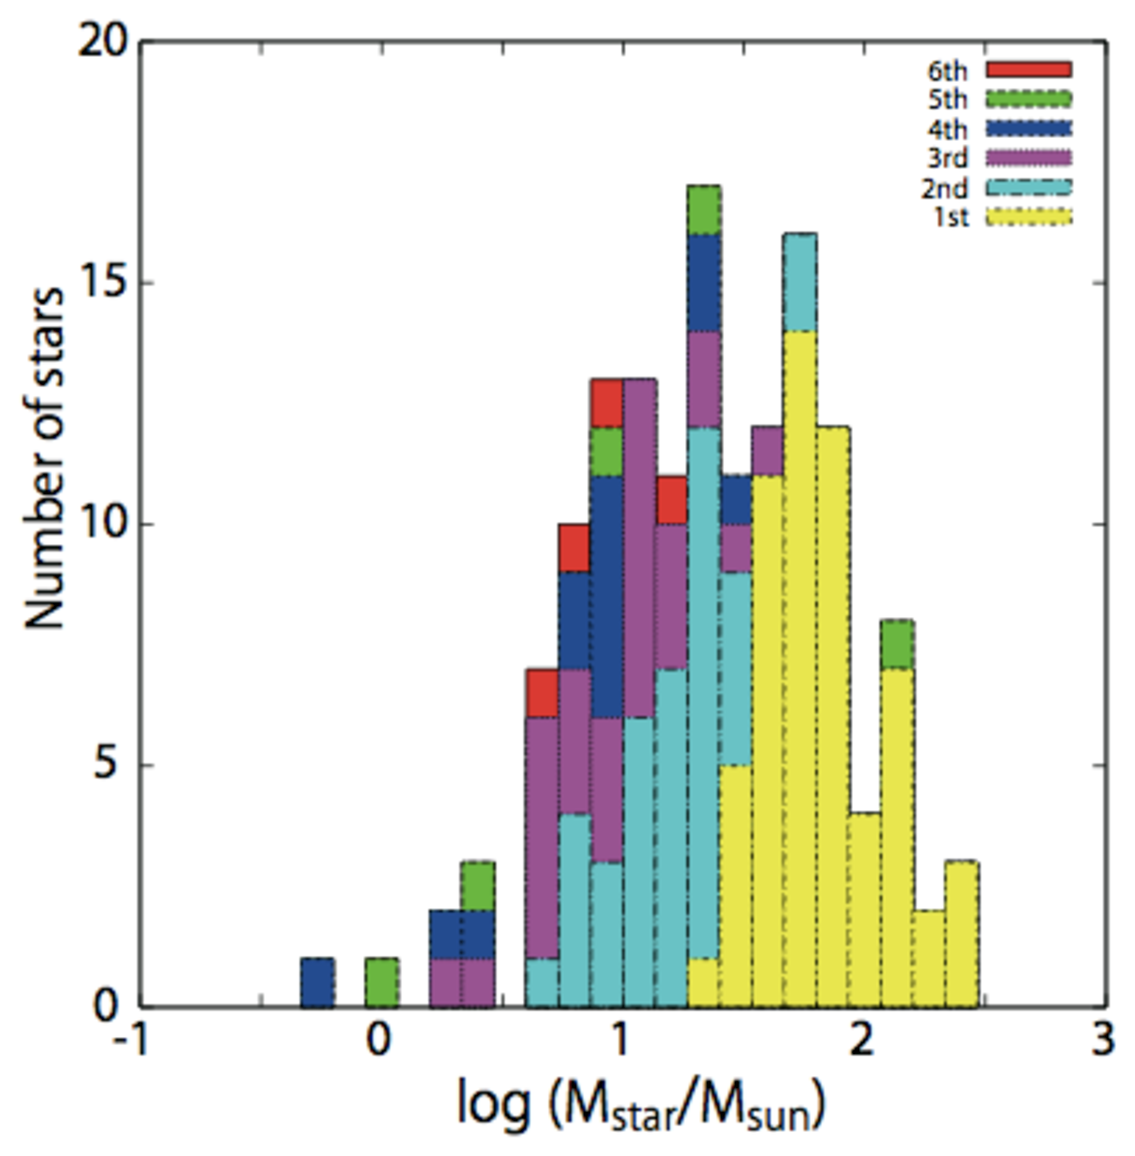
\includegraphics[width=8cm]{EoR/c03/c03.s2.f3.eps}}
	\caption{$B%7%_%e%l!<%7%g%s$K$h$C$FF@$i$l$?=iBe@1=i4|<ANL4X?t$N0l(B
 $BNc(B \citep{2014ApJ...792...32S}$B!#$3$N7W;;$G$O!"E57?E*$K$O(B$10-100M_\odot$$B!"3d9g$O>/$J$$$,(B$>100M_\odot$$B$d(B$<10M_\odot$$B$N=iBe@1$bB8:_!#$*$h$=(B1/3$B$,C1FH@1!"$=$l0J30$G$OJ#?t$N@17O$H$7$FCB@8!#(B}\label{KH3}
\end{figure}

\begin{figure}[!h]
	\centering\vspace*{1cm}
	{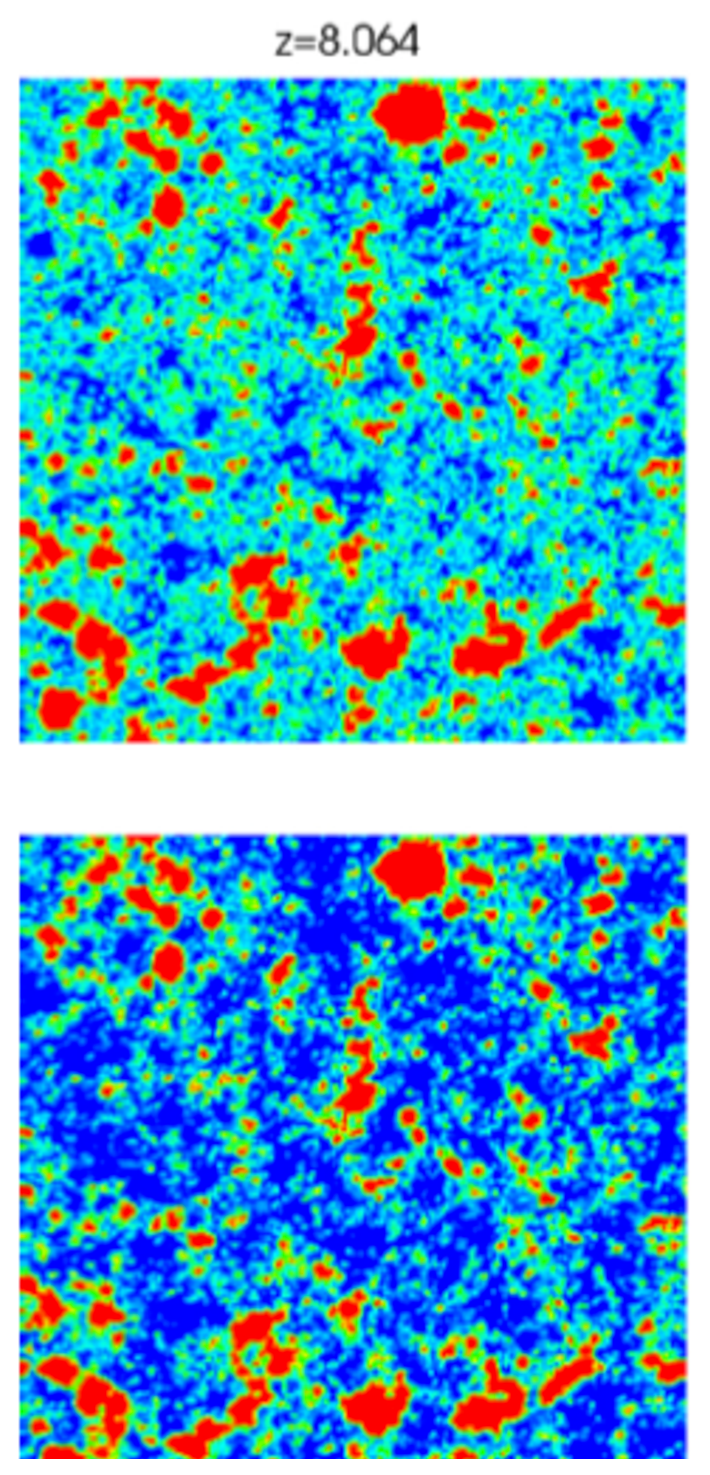
\includegraphics[width=5cm,angle=90]{EoR/c03/c03.s2.f4.eps}}
	\caption{$B%_%K%O%m!<$r9MN8$7$?>l9g(B($B:8?^(B)$B$H9MN8$7$J$$>l9g(B($B1&?^(B)$B$N(B
 $B@VJ}JP0\(B$z\approx8$$B$G$NEEN%9=B$(B($B@V$,EEN%NN0h!"@D$,Cf@-NN0h(B)$B!#%_%K%O%m!<(B
 $B$r9MN8$7$?>l9g!"ItJ,EEN%$5$l$?NN0h(B($BNP$NNN0h(B)$B$,@j$a$kBN@Q$,B?$/$J$j!"%H(B
 $B%`%=%s;6Mp$N8w3XE*8|$,A}2C$9$k(B \citep{2012ApJ...756L..16A}$B!#(B}\label{KH2} 
\end{figure}

EoR$B$N=i4|CJ3,$d(BCD$B$O!"=iBe@17A@.$K$h$C$F;O$^$k!#=iBe@1$O!"%_%K%O%m!<(B
($T_{\rm vir}<10^4$K, $B$b$7$/$O(B $10^4<M/M_\odot < 10^{7-8}$)$BFb$G@8$^$l$k$H?.$8$i(B
$B$l$F$$$k$,!"$3$N:]!"=iBe@1$N7A@.$O<g$K?eAGJ,;RNd5Q$K$h$C$F0z$-5/$3$5$l!"(B
$B8=:_$N@1(B($B<oB2(BI$B@1(B)$B$H$O0[$J$j=E85AG$r4^$^$J$$;v$+$i<oB2(BIII$B@1(B(Population
III star)$B$H$b8F$P$l$k(B\footnote{$B=E85AG$r4^$^$J$$@1$G$"$C$F$b!"@17A@.NN0h$,(B
$BEEN%!&2rN%mU<M$N1F6A$r<u$1$F$$$J$$>l9g$K$O<oB2(BIII.1$B@1!"$3$l$i$N1F6A$r<u$1(B
$B$?8e$K7A@.$5$l$k<!@$Be$N@1$O<oB2(BIII.2$B@1$H6hJL$9$k(B
\citep{2008AIPC..990.....O}$B!#$=$N0UL#$G!"<oB2(BIII$B@1$H=iBe@1$NDj5A$O87L)$K(B
$B$O0lCW$7$J$$!#(B}$B!#(B

\begin{figure}[!t]
	\centering
	{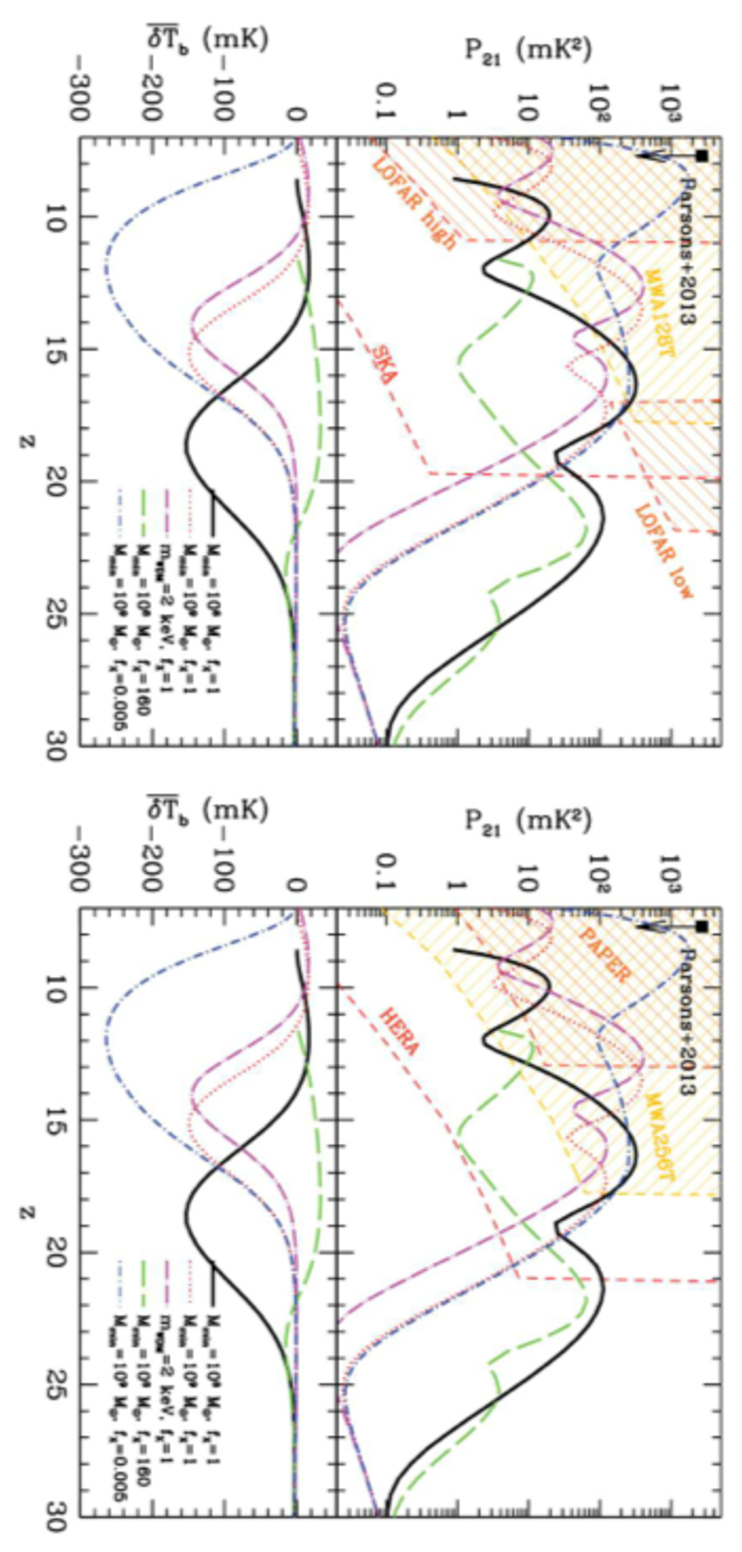
\includegraphics[width=5cm, angle=90]{EoR/c03/c03.s2.f5.eps}}
	\caption{$B>eCJ(B: $k=1/\rm Mpc$$B$K$*$1$k5eJ?6Q$7$?%Q%o!<%9%Z%/%H%k(B$P_{21}$$B$N?J2=(B $B!#$3$3$G!"(B$P_{21}$$B$O!"(B$P_{21}\equiv k^3/(2\pi^2V) \overline{\delta T_b}(z)^2\langle |\delta_{21}({\bf k},z)|^2 \rangle_k $$B!"(B$\delta_{21}({\bf x},z)=\delta T_b({\bf x},z)/\overline{\delta T_b}(z)-1$$B$GDj5A$5$l$k!#2<CJ(B: $BJ?6Q(B$\delta T_b$$B$N?J2=(B}\label{KH4}
\end{figure}
\begin{figure}[!h]
	\centering
	{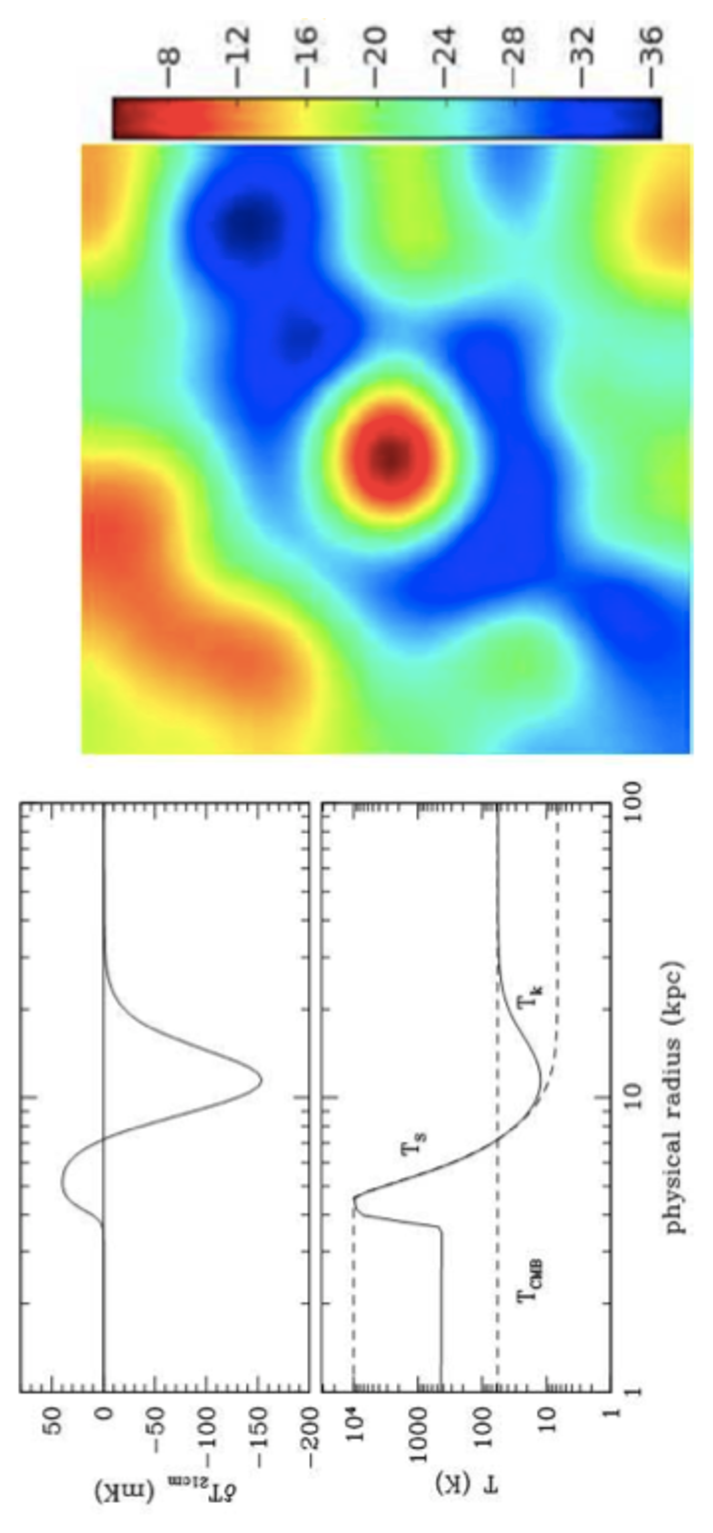
\includegraphics[width=5cm, angle=270]{EoR/c03/c03.s2.f6.eps}}
	\caption{$B:8?^(B: $BM}A[$J>u67$G$N<oB2(BIII$B@1(B + X$B@~8;$r4^$`6d2O<~$j$N%,(B
 $B%929EY(B($BGK@~(B)$B$H%9%T%s29EY(B($B<B@~(B)($B2<CJ(B)$B$H(B$\delta T_b$($B>eCJ(B) \citep{2008ApJ...684...18C}$B!#1&?^(B: $B$"$k$R$H$D$N1'ChO@E*L)EY%T!<%/(B $B$G7A@.$5$l$?L)=8$7$?6d2OFb$K<oB2(BIII$B@1(B + X$B@~O"@1(B + $B<oB2(BII$B@1$,B8:_$7$?>l9g$N(B$\delta T_b$$BJ,I[(B \citep{2014arXiv1405.2085A}$B!#(B $B%7%_%e%l!<%7%g%sNN0h%5%$%:$O!"0lJU(B40 comoving Mpc$B$G(B, $B%S!<%`I}(B $\Theta=2'$$BAjEv$NJ?3j2=$r9T$C$?8e$N?^$G$"$k!#?^Cf?4$NL)EY%T!<%/%5%$%:$O(B$\sim7$Mpc$\sim 10'$$B$KAjEv$9$k!#:8?^$G$O!"EEN%NN0h$9$030(B($BEEN%GHLL(B)$B$G2CG.$K$h$k51@~NN0h(B, $B$=$N$^$o$jNd$?$$%,%9$K$h$k5[<}NN0h$,8+$($k!#1&?^$G$O(B$\delta T_b>0$$B$N51@~NN0h$,8+$($J$$$,!"%S!<%`I}$r>.$5$/$7$?>l9g(B($B6u4VJ,2rG=$r>e$2$?>l9g(B)$B$K$O8+$($k2DG=@-$b$"$k!#(B}
	\label{KH5}
\end{figure}

2000$BG/:"$h$j?tCM%7%_%e%l!<%7%g%s$K$h$k=iBe@17A@.$N8&5f$,3hH/$K$J$j!"Bg<A(B
$BNL(B($\ge100M_\odot$)$B$N<oB2(BIII$B@1$,8IN)$7$F7A@.$5$l$k!"$$$o$f$k!H(Bone Pop III
star per one minihalo$B!I%Q%i%@%$%`$,?.$8$i$l$F$-$?(B(e.g.,
\cite{2002Sci...295...93A, 2002ApJ...564...23B, 2006ApJ...652....6Y}) $B!#(B
$B6aG/$G$O!"B??t$N%_%K%O%m!<%5%s%W%k$rMQ$$$?%7%_%e%l!<%7%g%s$K$h$C$FI}9-$$(B
$B<oB2(BIII$B@1<ANL$,<B8=$5$l$k;v$b<($5$l(B(e.g., \cite{2014ApJ...781...60H},
\cite{2014ApJ...792...32S})$B!"0l$D$N%_%K%O%m!<Fb$GJ#?t$NHf3SE*7Z$$(B
($10-100M_\odot$)$B@1$,@8$^$l$k2DG=@-$b;XE&$5$l$F$$$k(B(e.g.,
\cite{2009Sci...325..601T, 2010MNRAS.403...45S, 2011ApJ...737...75G,
2014ApJ...792...32S}, $B?^(B\ref{KH3})\footnote{$B6aG/$N798~$H$7$F$O%_%K%O%m!<(B
$BFb$N%,%9J,Nv$O5/$3$j$&$k$H$$$&8+J}$,B?$$!#$7$+$7!"$=$l$iJ,NvJR$,@1$K$J$k(B
$B$+!"$b$7$/$O$=$N$^$^Cf?4@1$K9_Ce$9$k$+$O$^$@5DO@$,<}B+$7$F$$$J$$!#(B}$B!#<oB2(B
III$B@1$N=i4|<ANL4X?t(B(Initial Mass Function: IMF) $B$O!"$3$l$i@1$+$i$NJ|<M$N(B
$B%9%Z%/%H%k%(%M%k%.!<J,I[(B(Spectral Energy Distribution: SED)$B$N9E$5(B
(hardness)$B$K4XO"$9$k!#$^$?!"(BX$B@~O"@1$,7A@.$5$l$k>l9g!"(BX$B@~$NBg$-$JJ?6Q<+M3(B
$B9TDx$K$h$j!";g30@~$GEEN%$5$l$k>l9g$HHf$Y$F$J$a$i$+$JEEN%9=B$$,$G$-$k$H9M(B
$B$($i$l$k(B \citep{2013MNRAS.431..621M}$B!#$3$N$h$&$K!"<oB2(BIII$B@1$N(BIMF$B$d7A@.N($O(B
$BEEN%9=B$$NH/C#$HL)@\$K4XO"$9$k!#(B



$B$7$?$,$C$F!"=iBe@17A@.!&?J2=$NM}O@$O(BCD, EoR$B$N%b%G%j%s%0$N:]$K=EMW$H$J$k!#(B
$B=iBe@17A@.$K$*$$$F!"<g$K$=$N7A@.$rAK32$9$k$N$O(BLyman-Werner$B%P%s%ImU<M$K$h(B
$B$k?eAGJ,;R$N8w2rN%$G$"$j(B(e.g., \cite{2000ApJ...534...11H})$B!"6aG/$G$O!"$3(B
$B$N?eAGJ,;R2rN%8w;R$NmU<MM"Aw$b9MN8$7$?BgNN0h(B($\ge 100$Mpc)$B:FEEN%%7%_%e%l!<(B
$B%7%g%s$b$J$5$l$F$$$k(B (\cite{2012ApJ...756L..16A} $B?^(B\ref{KH2})$B!#(B 



$B$^$?6aG/$G$O!"@2$l>e$,$j4|$K$*$1$k%P%j%*%s$H%@!<%/%^%?!<$NB.EY:9$N8z2L$b(B
$BE7BN7A@.2aDx$K1F6A$rM?$($k$H9M$($i$l$F$$$k(B \citep{2010PhRvD..82h3520T}$B!#(B
$B$3$N8z2L$r9MN8$7$?>l9g!"@17A@.2DG=$J%_%K%O%m!<<ANL$,Bg$-$/$J$j!"%O%m!<$N(B
$B7A@.;~4|$bCY$/$J$k;v$,?tCM%7%_%e%l!<%7%g%s$K$h$C$F<($5$l$F$$$k(B
 \citep{2011ApJ...730L...1S, 2011ApJ...736..147G}$B!#$^$?!"$3$NB.EY:9$N8z2L(B
$B$O!">W7bGH$h$C$FBg6IE*$J2CG.$r0z$-5/$3$9;v$G(B21 cm $B%Q%o!<%9%Z%/%H%k$K1F6A(B
$B$rM?$($k;v$b9M$($i$l$k(B \citep{2012ApJ...760....3M}$B!#(B

CD$B$H(BEoR$B$K$*$1$k(B21 cm$B%Q%o!<%9%Z%/%H%k2r@O$K4X$7$F!";0$D$NFCD'E*$J;~4|$,$"(B
$B$k!#(B(1) IGM$B$N29EY$,!"(BWouthysen-Field$B8z2L$K$h$C$F(BLyman-$\alpha$$BmU<M$H6/$/(B
$B%+%C%W%k$9$k!V(BLyman-$\alpha$-pumping epoch$B!W(B, (2) IGM$B$,(BX$B@~$K$h$C$F2CG.$5(B
$B$l!"=y!9$K(BCMB$B29EY$rD6$($k!V(BX-ray heating epoch$B!W!"(B(3) $BEEN%%P%V%k$,1'ChO@(B
$BE*%9%1!<%k$G7A@.$5$l$k!V(BEpoch of Reionization$B!W!#$=$l$>$l$N;~4|$G!"(B21 cm
$B51EY29EY(B ($\delta T_b\equiv{(T_{\rm
s}-T_{\gamma}(z))}(1-e^{-\tau_{21}})/(1+z))$)$B$N?6I}$d6u4VMI$i$.$OA}I}$5$l(B
$B$k(B (\cite{2014MNRAS.439.3262M}, $B?^(B\ref{KH4})$B!#(B 

$B:$Fq$G$O$"$k$,!"%H%b%0%i%U%#!<(B($B3F@VJ}JP0\$G$N;#A|(B)$B$O=iBe6d2O$[$I>.$5$JE7(B
$BBN$rJ,2r$G$-$k$+$b$7$l$J$$!#=iBe6d2O$NJ|<M%9%Z%/%H%k$O!"6d2OFb$N@1<ANL4X(B
$B?t$d(BX$B@~8;$NM-L5$J$I$K$h$C$F7hDj$5$l$k$,!"$3$NJ|<M%9%Z%/%H%k$N7A$O<~JU$N(B
$BEEN%9=B$!"(B21 cm$B%9%T%s29EYJ,I[$K1F6A$rM?$($k!#$b$7!"=iBe6d2O<~0O$N(B21 cm$B%7%0(B
$B%J%k$,8!=P$G$-$l$P=iBe6d2O$NFCD'$K@)8B$,IU$1$i$l$k$+$b$7$l$J$$(B(e.g.,
\cite{2008ApJ...684...18C, 2014arXiv1405.2085A})$B!#(B 
$BNc$($P!"Nd$?$$6d2O4V%,%9Fb$K;g30@~$H(BX$B@~$NJ|<M8;$,B8:_$9$k>l9g$r9M$($k(B($B?^(B
\ref{KH5}$B:8(B)$B!#J|<M8;IU6a$G$O!"2CG.$K$h$C$F%,%929EY$,(BCMB$B29EY$r>e2s$k$,!"EE(B
$BN%NN0hFb$G$OCf@-?eAG3d9g$,Hs>o$K>.$5$$0Y!"(B21 cm$B$N%7%0%J%k$O8+$($J$$(B
($\delta T_b\approx0$)$B!#$7$+$7!"$=$N30B&$NEEN%GHLL$KAjEv$9$kItJ,$G(B
$B$O!"Cf@-?eAG$,;D$C$F$*$j!"$+$D!"2CG.$K$h$C$F%,%929EY$,(BCMB$B29EY$r>e2s$k0Y!"(B
21 cm$B51@~(B($\delta T_b>0$)$BNN0h$,8=$l$k!#$h$j30B&$G$O!"Dc29%,%9$G$"$k(B
$B$?$a(B21 cm$B5[<}(B($\delta T_b<0$)$BNN0h$,8=$l$k$,!"$5$i$K30B&$G$O!"(BWF$B8z2L(B
$B$K$h$k%,%929EY$H%9%T%s29EY$N%+%C%W%j%s%0$,==J,$K5/$3$i$:!"(B21 cm$B%7%0%J%k$O(B
$B8+$($J$/$J$k!#0J>e$N$h$&$J?6$kIq$$$O!"J|<M%9%Z%/%H%k$N$+$?$A$K$h$C$F0c$$(B
$B$,@8$8$k!#Dj@-E*$K$OJ|<M%9%Z%/%H%k$r$h$j9E$/$9$k$[$I!"51@~NN0h$,9-$,$j5[(B
$B<}NN0h$,8+$($J$/$J$k798~$H$J$k!#(BAhn$B$i$O!"1'ChO@E*%7%_%e%l!<(B
$B%7%g%s$K$h$C$F$h$j8=<BE*$J>u672<$GL)=8$7$?6d2O<~0O$N(B$\delta T_b$$BJ,I[$rMM!9(B
$B$r7W;;$7!"6d2OJ|<M%9%Z%/%H%k$K$h$k(B21 cm$B%7%0%J%kJ,I[$N0c$$$r5DO@$7$F$$$k(B
(\cite{2014arXiv1405.2085A}, $B?^(B\ref{KH5}$B1&(B)$B!#(B 
%初代銀河、Lyman-$\alpha$とX線強度の揺らぎ、スピン温度
\subsection{SKA1-low$B$K$h$k:FEEN%4|$NEEN%NN0h$N;#A|(B}
\label{c03.s2.ss4}
\subsubsection{$BF3F~(B}
$B:FEEN%4|$K$*$1$k6d2O4VJ*<A$NEEN%9=B$$N;#A|$O!"(BSKA$B$NL\I8$N0l$D$G$"$k!#:FEE(B
$BN%4|$NEEN%NN0h$N9=B$$O!"L$$@$h$/2rL@$G$-$F$$$J$$6d2O7A@.$NJ*M}$KIR46$G$"(B
$B$k0Y!"EEN%9=B$$N%9%1!<%k$d?J2=$r;#A|$9$k;v$,$G$-$l$P!"MM!9$J6d2O7A@.%7%J(B
$B%j%*$N6hJL$d8w8;$NJ|<M%9%Z%/%H%k%?%$%W$N6hJL$,2DG=$H$J$k!#$3$3$G$O!"$=$N(B
$B0Y$N6qBNE*$J<jK!$r@bL@$9$k!#(B

SKA$B$N@h6nBN(B(precursor)$B$G$"$k(BMWA$B$d(BLOFAR$B$G$O46EY$,Dc$$$N0Y!"%Q%o!<%9%Z%/%H%k(B
$BEy$NE}7WE*4QB,$,%a%$%s$H$J$k!#0lJ}$G!"(BSKA1-low$B$G$O!"(Bi) 21 cm$B51@~$H6d2O$NAj(B
$B8_Aj4X(B(e.g., \cite{2007ApJ...660..1030F, 2007MNRAS.375..1034W}), ii) $BmU(B
$B<M6/EYMI$i$.$N3NN(J,I[(B(e.g., \cite{2009MNRAS.397..1138H,
2009MNRAS.397..1454B}), iii) $B8D!9$NEEN%NN0h(B, iv) $B%/%(!<%5!<$,;YG[E*$J(BHII
$BNN0h$J$I$N4QB,(B(e.g., \cite{2004Natur.432..194W, 2005ApJ...633..552K,
2006MNRAS.369L..66V})$B$,2DG=$K$J$k$H4|BT$5$l$k!#(B

21 cm signal$B$H6d2O$NAj8_Aj4X$+$i$O!"(B"outside-in"($BDcL)EYNN0h$,@h$KEEN%$9$k%7(B
$B%J%j%*(B)$B$H(B"inside-out"($B9bL)EYNN0h$,@h$KEEN%$9$k%7%J%j%*(B)$B:FEEN%$,6hJL$G$-$k!#(B
$BDL>o!"6d2O$rEEN%8w;R8;$H$7$?%7%_%e%l!<%7%g%s$G$O!"9bL)EYNN0h$,@h$KEEN%$9(B
$B$k!#$3$N>l9g!"6d2OJ,I[$H(B21 cm$B%7%0%J%k$O5UAj4X$r<($9$H4|BT$5$l$k!#(B


\subsubsection{$B=`?tCME*:FEEN%7W;;(B} 

$B=`?tCME*%b%G%k$N$R$H$D$G$"$k(BGALFORM$B$K!"4JN,2=$7$?<h$j07$$$G$NEEN%9=B$7W;;(B
$B$rAH$_9~$`(B(e.g., \cite{2013MNRAS.428..2467K})$B!#$3$N7W;;$G$O!"EEN%8w;R8;<~(B
$B$j$G$NEEN%8w;RJ|<MN($K1~$8$FEEN%NN0h$r7A@.$7!"6aK5EEN%NN0h$N%*!<%P!<%i%C(B
$B%W$O8w;R?t$NJ]B8$r9MN8$7$FL7=b$J$/07$o$l$k!#$^$?!"EEN%8w;R8;$H$7$FMM!9$J(B
$B6d2O%b%G%k$rAH$_9~$`$3$H$,2DG=$G$"$k!#(B

\subsubsection{$BEEN%NN0h$H6d2O7A@.(B}$B!!(B

$BD6?7@1GzH/$K5/0x$9$k%"%&%H%U%m!<$K$h$k@17A@.AK32$"$j$N>l9g(B($BD6?7@1GzH/%U%#!<(B
$B%I%P%C%/%b%G%k(B)$B$HL5$7$N>l9g$G$N!"=`?tCME*:FEEN%7W;;7k2L$NHf3S$r<($9!#D6?7@1GzH/%U%#!<%I%P%C%/%b%G%k(B
$B$G$O!"Dc<ANL6d2O7A@.$,AK32$5$l!"Bg<ANL6d2O$KJP$C$?8wEY4X?t$K$J$C$F$*$j!"(B
$B$=$l$>$l$N%b%G%k$G$N6d2O$N8wEY4X?t$O!"4QB,$r:F8=$9$k$h$&$K%b%G%k2=$5$l$F(B
$B$$$k(B($BL@$k$$ItJ,$7$+4QB,$HHf3S$G$-$J$$$N$G!"0E$$ItJ,$OG$0U@-$r;}$?$;$k;v$,(B
$B$G$-$k(B)$B!#$3$N7W;;$G$O!"3F;~4|$K$*$1$k6d2O4VJ*<A$NJ?6QCf@-?eAG3d9g$O8_$$$K(B
$BEy$7$/$J$k$h$&$KD4@0$5$l$F$$$k!#$9$J$o$A!"$U$?$D$N%b%G%k$N0c$$$O!"!V$"$k(B
$BJ?6QEEN%EY$rC#@.$7$?$H$-!"EEN%8w;R8;$H$7$F!">.<ANL6d2O$,;YG[E*$+Bg<ANL6d2O$,(B
$B;YG[E*$+!W$H$J$C$F$$$k!#$=$N7k2L!"J?6QCf@-?eAG3d9g$OF1$8$G$bEEN%NN0h$N%5(B
$B%$%:J,I[$OBg$-$/0[$J$k(B($B?^(B\ref{KH7})$B!#Dc<ANL6d2O$,;YG[E*$J>l9g!"B??t$N>.%9(B
$B%1!<%k(BH{\textsc{ii}}$BNN0h$,8=$l$k(B \citep{2013MNRAS.428..2467K}$B!#(B
\begin{figure}[!t]
	\centering
	{\includegraphics[width=10cm, angle=90]{EoR/c03/c03.s2.f7.eps}}
	\vspace{-1cm}
	\caption{GALFORM$B$rMQ$$$?(B500Mpc$B7W;;NN0h$N7W;;7k2L!#:8?^(B: $BD6?7@1Gz(B
 $BH/%U%#!<%I%P%C%/$r(B
	$B9MN8$7$?>l9g!"1&?^(B: $BD6?7@1GzH/%U%#!<%I%P%C%/$rL5;k$7$?>l9g!#(BKim et al. in prep.}\label{KH7}
\end{figure}

%\subsubsection{$B%/%(!<%5!<<~0O$NCf@-?eAG(B}$B!!(B%
%$B$$$/$D$+$N@VJ}JP0\(B$z\sim6$$B$N%/%(!<%5!<<~JU$G$O!"ItJ,E*$KCf@-$JEEN%NN0h$N(B
%$BB8:_$,<(:6$5$l$k!#:G6a$G$O!"(B$z\sim7$$B$N%/%(!<%5!<<~0O$G6d2O4VJ*<A5/8;$N(B
%Lyman-$\alpha$ damping wing$B$,8!=P$5$l!"Cf@-%,%9$,B8:_$r<($9$h$j6/$$>Z5r(B
%$B$H$J$C$?(B \citep{2011MNRAS.416L..70B}$B!#(B 
%14/12/6 $B>JN,(B($B!v:G6a$G$O!"(B$z\sim6$ QSOs$B$N%9%Z%/%H%k$K$b(BGP trough$B$,$_$D$+$j!"Cf@-?eAG$NB8:_$r<(:6(B, Becker et al. (2014)$B!#(BTotani et al. 2014$B$G$O!"(BGRB afterglow$B$N5[<}@~7O$N2r@O$+$i(B$z\sim5.8$$B$GCf@-?eAG$,;D$C$F$$$k;v$r<(:6!#(BSKA$B$G$3$N$h$&$J>l=j$r4QB,$G$-$l$P!"(B21 cm$B$N%7%0%J%k$,4|BT$G$-$k(B?)
%\\\\
%{\bf SKA1-low$B$N;#A|46EY(B}
% $B$3$N@a$O!"<($5$l$F$$$kCM$N;29MJ88%$bM?$($i$l$F$*$i$:!"?.Mj@-$,ITL@$J$N$G$6$C$/$j>JN,$7$^$9!#(B
%$B$3$3$G$O!"Ds0F$5$l$$$k(BSKA1-low$B$N%Y!<%9%i%$%s%G%6%$%s$N:FEEN%4|$NEEN%NN0h;#A|$KBP$9$k46EY$r8+@Q$b$k!#(BSKA1-low$B$O!"(B866$B$N%9%F!<%7%g%s$G9=@.$5$l!"$=$l$>$l(B45m$B$N%9%F!<%7%g%sFb$K(B256$B$N%"%s%F%J$,B8:_$9$k!#$3$3$N2r@O$G$O!"H>7B(B650$B%a!<%H%kFb$K0lMM$K%"%s%F%J$,CV$+$l$F$$$k$H2>Dj$9$k!#(B$\nu<200\rm MHz$$B$G$N%7%9%F%`29EY$O(B$T_{sys}\approx 250[(1+z)/7]^{2.6}$K$B$G$"$k!#$3$N(Bconfiguration$B$G$N3QEYJ,2rG=$O!"$3$N?6F0?t$G$*$h$=(B5.4 arcmin$B$G$"$j!"(Bprimary beam width$B$O(B$\theta_b=3.4$ degrees$B$H$J$k!#7k2L$H$7$F(Brms noise $B$O!"(B
%\begin{equation}
%\Delta T_b \approx 0.9 {\rm mK} \left(\frac{1+z}{8.5}\right)^{2.6}\left(\frac{\Delta \nu}{1{\rm MHz}}\frac{t_{int}}{1000{\rm hr}}\right)^{-1/2} \left(\frac{\theta_b}{6'}\right)^{-2}
%\end{equation}
%$B$H$J$k!#(B\\\\

\subsubsection{$B%7%_%e%l!<%7%g%s7k2L$N(BSKA1-low$B$K$h$kLO5<4QB,(B}
\begin{figure}[!t]
	\centering
	{\includegraphics[width=9cm, angle=90]{EoR/c03/c03.s2.f8.eps}}
	\vspace{-0.8cm}
	\caption{SKA1-low$B$G$N%7%_%e%l!<%7%g%s7k2L$NLO5<4QB,!#$3$3$G$O!"D6?7@1GzH/%U%#!<%I%P%C%/(B
	$B$,8z2LE*$KF/$$$?>l9g$N7k2L$r<($9!#(B
	$B:8>e?^!'%7%_%e%l!<%7%g%s7k2L!#(B
	$B1&>e?^!'A07JJ|<M$J$7$NLO5<4QB,!#(B
	$B:82<?^!'A07JJ|<M9~$_$G!"(BSKA-1 low$B$K$h$k(B1000$B;~4V4QB,$r2>Dj!#(B
	$B1&2<?^!'46EY$r(B1/2$B$K$7$?>l9g$NLO5<4QB,?^!#(B}\label{KH8}
\end{figure}
\begin{figure}[!h]
	\centering
	{\includegraphics[width=9cm, angle=90]{EoR/c03/c03.s2.f9.eps}}
	\vspace{-0.8cm}
	\caption{$B?^(B8$B$HF1MM$@$,!"D6?7@1GzH/%U%#!<%I%P%C%/$rL5;k$7$?>l9g$N7W;;7k2L$NLO5<4QB,(B}
	\label{KH9}
\end{figure}
$BD6?7@1GzH/%U%#!<%I%P%C%/$r9MN8$7$?7W;;NN0h(B$(1 {\rm Gpc}/h)^3$$B$N%7%_%e%l!<(B
$B%7%g%s$N7k2L$r(BSKA1-low$B$GLO5<4QB,$r$9$k(B($B;29MJ88%$OL$Ej9F(B)$B!#A07JJ|<M$H$J$k(B
$B6d2O7OFb%7%s%/%m%H%m%sJ|<M$d7O306d2O$NJ|<M$O:FEEN%4|$N(B21 cm$B%7%0%J%k8!=P$NBg(B
$B$-$J>c32$H$J$k!#$3$3$G$O!"J,2r2DG=E7BN$N$+$i$NJ|<M$OA4$F<h$j=|$1$?$H2>Dj(B
$B$9$k!#?^(B\ref{KH8}$B$O!"(BSKA1-low$B$G(B1000$B;~4V4QB,$r2>Dj$7!"A07JJ|<M=|5n(B
 \citep{2008MNRAS.390..1496G, 2011MNRAS.418..516G}$B8e$NLO5<4QB,%^%C%W$G$"(B
$B$k!#7k2L!"D6?7@1GzH/%U%#!<%I%P%C%/$,8z2LE*$G$"$k>l9g$K@8@.$5$l$kEEN%NN0h(B
$B$N;#A|$O2DG=$G$"$m$&!#(B 

$B0lJ}$G!"D6?7@1GzH/%U%#!<%I%P%C%/$J$7$N%b%G%k$N>l9g!":G$bBg$-$JEEN%NN0h$O(B
$B4QB,$G$-$=$&$@$,!"<B:]$K$O%N%$%:$HA07JJ|<M=|5n$K$h$C$FEEN%NN0h$N%3%s%H%i(B
$B%9%H$,2<$2$i$l$k$?$a!"(BSKA1-low$B$G$N;#A|$O:$Fq$G$"$m$&(B($B?^(B\ref{KH9})$B!#(BSKA2
$B$G$O(B4$BG\DxEY46EY$,NI$$0Y!";#A|$G$-$k2DG=@-$,$"$k!#(B



% \subsubsection{$B:FEEN%4|$NEEN%GHLL$N4v2?3XE*8|$_(B}
% $B%/%(!<%5!<$O!"@17A@.6d2O$KHf$Y$F9E$$J|<M%9%Z%/%H%k;}$D$?$a!"4v2?3XE*$K8|(B
% $B$$EEN%GHLL$r;}$D!#EEN%GHLL$G$O!"29EY$,9b$/ItJ,EEN%$7$??eAG$,;D$C$F$$$k$?(B
% $B$a!"(B$\delta T_b>0$$B$H$J$j!"$h$j30B&$G$ONd$?$$6d2O4V%,%9$K$h$j(B$\delta
% T_b<0$$B$H$J$k!#$3$l$K$h$j!"EEN%GHLL$N8|$5$rJ,2r$G$-$k$[$I==J,$J6u4VJ,2rG=(B
% $B$,$"$l$P!"EEN%GHLLIU6a$N(B21 cm$B%7%0%J%k$rD4$Y$k;v$G$I$N$h$&$JE7BN$,8w8;$G$"(B
% $B$k$+6hJL$9$k;v$,$G$-$k!#(B

%{\bf SKA1-low$B$N;kLn(B}
%$B%7%_%e%l!<%7%g%s$O!":FEEN%$N8e4|CJ3,$K$*$$$F(B100Mpc($\sim$1$BEY(B)$B0J>e$N6u4V%9%1!<%k$NCf@-NN0h$NB8:_$rM=8@$9$k!#(B\\\\

\subsubsection{$B$^$H$a(B} 

$B6d2O%b%G%k$N0c$$$K$h$C$F4|BT$5$l$kEEN%9=B$$,Bg$-$/0[$J$k$?$a!"$b$7(B21 cm$B%7(B
$B%0%J%k$N6u4VJ,I[$r4QB,$G$-$l$P!"Nc$($PD6?7@1GzH/$K$h$k%U%#!<%I%P%C%/$,8z(B
$B2LE*$KF/$$$F$$$k$+$I$&$+$J$I$N6d2O7A@.$NJ*M}$rM}2r$9$k;v$,$G$-$k!#(B
SKA1-low$B$N>l9g!"6/$$D6?7@1GzH/%U%#!<%I%P%C%/$,8z2LE*$KF/$$$F$$$l$P$G$NEE(B
$BN%NN0h$OJ,2r$G$-$k!#$7$+$7!"D6?7@1GzH/$N%U%#!<%I%P%C%/$,8z2LE*$G$J$/!"Dc(B
$B<ANL6d2O$K$h$kEEN%8w;R6!5k$,;YG[E*$G$"$k>l9g!"$h$j9b$$6u4VJ,2rG=$,I,MW$H(B
$B$J$k!#EEN%NN0h$rJ,2r$G$-$k9b$$J,2rG=$K2C$($F!":G$bBg$-$JEEN%9=B$(B($B$3$N7W;;(B
$B$G$O(B$100$Mpc$B$G$*$h$=(B1$BEY$N3QEY$KAjEv(B)$B$N;#A|$r$9$k0Y$K$O!"(BSKA1-low$B$N;kLn$O>/(B
$B$J$/$H$b?tEY$OI,MW$G$"$k!#(B
%SKA1-lowによる再電離期の電離領域の撮像
\subsection{$B;#A|4QB,(B}
\label{c03.s2.ss5}

$B:FEEN%4|$N4QB,$G$O(B 21 cm$B@~$N51EY29EY$,F@$i$l$k!#(B21cm$B@~$N51EY29EY$r2r@O$7$F!"(B
$B:FEEN%4|$NJ*M}$d=i4|E7BN$K$D$$$F$N>pJs$rF@$k;v$,$G$-$k!#2r@O$N<jK!$H$7$F!"(B
$BE}7WE*<jK!$H;#A|$,$"$k!#E}7WE*<jK!$H$7$FBeI=E*$J$b$N$O%Q%o!<%9%Z%/%H%k$K(B
$B$h$k2r@O$G$"$k!#(B21 cm$B@~$N51EY29EY$N;}$DMI$i$.$N>pJs$rE}7WE*$K=hM}$7!":FEE(B
$BN%4|$G$NJ*M}$K@)8B$r2C$($k!#0lJ}!";#A|$OE}7WE*$J=hM}$G$O$J$/!"F@$i$l$?(B
21cm$B@~$N%7%0%J%k$+$iA|$r9g@.$7!":FEEN%4|$NMM;R$rD>@\8+$h$&$H$9$k$b$N$G$"(B
$B$k!#$3$N@a$G$O;#A|$K$h$C$F:FEEN%4|$N2?$,J,$+$k$H9M$($i$l$F$$$k$+$^$H$a$k!#(B 

$B;#A|$r9T$&$K$O!"EEGH43>D7W$,==J,$J3QEYJ,2rG=$r$b$DI,MW$,$"$k!#$7$+$7!"4Q(B
$BB,$GJ,2rG=$r>e$2$k$H$$$&;v$O4QB,$KH<$&%N%$%:$N4sM?$r6/$/<u$1$k;v$K$J$k!#(B
$B%N%$%:$KBP$7$FM%0L$K%7%0%J%k$,F@$i$l$?$+$I$&$+$O!"(BS/N$B$r;H$C$FH=Dj$9$k!#(B
S/N$B$O4QB,CM$H4QB,8m:9$NHf$G$"$k!#;#A|$r9T$&$?$a$K$O$3$N(BS/N$B$,==J,$KBg$-$$(B
$BI,MW$,$"$k(B(1$B0J>e(B)$B!#%"%s%F%J$NM-8z3+8}LL@Q(B$ A_{eff}$$B$H%7%9%F%`29EY(B$
T_{sys}$$B$r8GDj$9$k$H!"(BS/N$B$O4QB,;~4V$d4QB,<~GH?t$N%A%c%s%M%kI}!"$=$7$F4Q(B
$BB,$NJ,2rG=$K0MB8$9$k!#?^(B\ref{yoshiura.fig:1}$B$O(BSKA$B$K$h$C$F;#A|$,$I$l$/$i(B
$B$$$NJ,2rG=$G2DG=$+$r<($7$?$b$N$G$"$k(B \citep{2013ExA....36..235M}$B!#(B21 cm$B@~(B
$B$N%7%0%J%k$,(B 1 mK$BDxEY$G$"$k$H$7$F(B($B<B:]:FEEN%4|$G$N51EY29EY$NBg$-$5$O(B 1mK
$BDxEY$H9M$($i$l$F$$$k(B)$B!"K>1s6@$K5a$a$i$l$k(B$ A_{eff}/T_{sys}$$B$r<($9$b$N$,(B
$B3%?'$NNN0h$G$"$k!#<P@~$G0O$^$l$?NN0h$O!"(BSKA($BCf?4$N%3%"$,H>7B(B2Km)$B$N<B8=2D(B
$BG=$J(B$ A_{eff}/T_{sys}$$B$G$"$j!"Cf$K$"$k(B3$BK\$N<B@~$O>e$+$iJ*M}E*3+8}LL@Q$,(B
$0.25~\rm km^2$,$1~\rm km^2$,$2.5~\rm km^2$$B$N>l9g$G$"$k!#$3$N<B@~$h$j2<$K!"(B
$B3%?'$NNN0h$,$"$l$P$=$NJ,2rG=$G$N;#A|$,2DG=$G$"$k$HM=A[$5$l$k!#(B 

\begin{figure}[t]
 \centering
 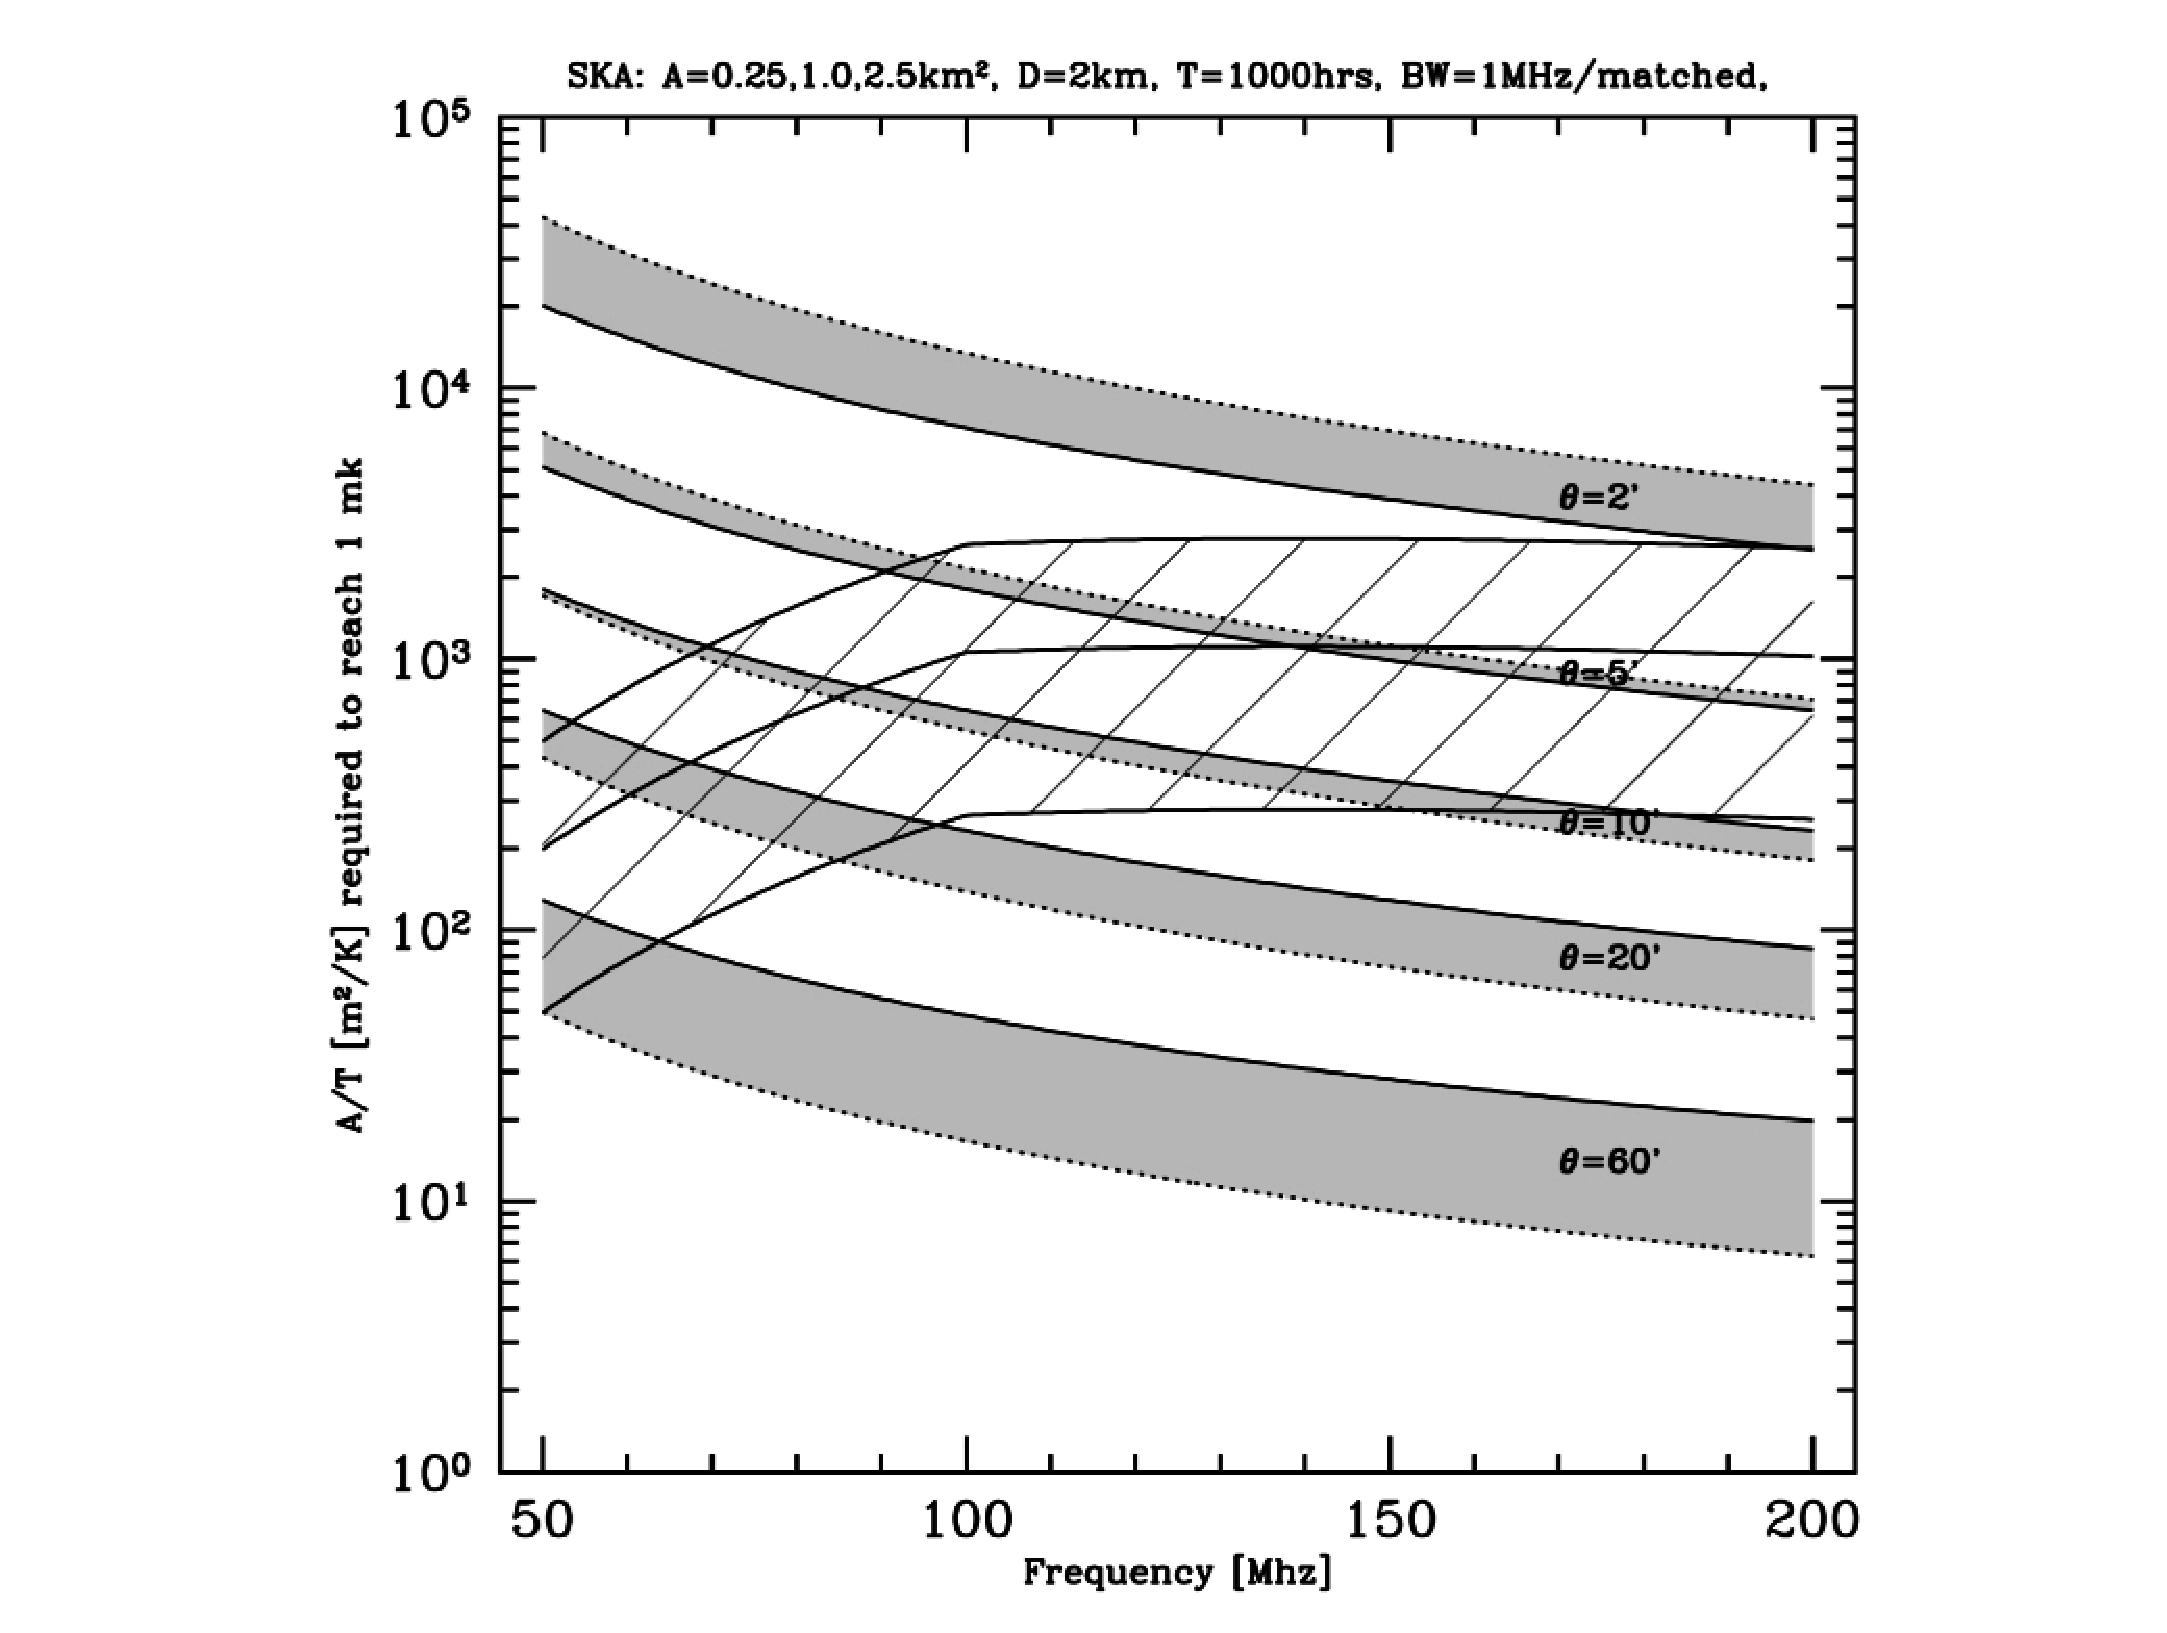
\includegraphics[width=10cm,clip]{EoR/c03/c03.s2.f10.eps}
 \label{yoshiura.fig:1}
\caption{1mK$B$N51EY29EY$+$i;#A|$9$k$?$a$K5a(B
 $B$a$i$l$k(B$A_{eff}/T_{sys}$$B$r<($7$F$$$k!#=D<4$,(B$ A_{eff}/T_{sys}$$B$NBg$-$5!"(B
 $B2#<4$,<~GH?t$G$"$k!#3%?'$N@~$,J,2rG=$4$H$K5a$a$i$l$k(B$ A_{eff}/T_{sys}$$B$NBg$-$5!"<P@~$O(BSKA$B$G<B8=2DG=$J(B$ A_{eff}/T_{sys}$$B$NBg$-$5$rI=$9!#<P@~$h$j2<$K2+?'$$@~$,$"$l$P(BSKA$B$G$N;#A|$,2DG=$G$"$k!#(B}
\end{figure}


\subsubsection{$B;#A|$K$h$k2r@O(B}
$B;#A|$K$h$C$F:FEEN%4|$G$N(B21cm$B@~$N%^%C%W$rF@$F!"<!$KLdBj$J$N$O$=$l$r$I$N$h$&$K2r@O$9$k$+!"$H$$$&;v$G$"$k!#$3$3$G$O8=:_9M$($i$l$F$$$k2r@O<jK!$r>R2p$9$k!#(B\\

(a)$B%$%*%s2=%P%V%k(B : $B;#A|$rMQ$$$?2r@O$G$O%$%*%s2=%P%V%k$N%5%$%:J,I[$dFC0[E7BN<~$j$NNN0h$r07$&!#(B
$B%$%*%s2=%P%V%k$H$OCf@-?eAG$,%$%*%s2=$5$l$?NN0h$N$3$H$G!";#A|$r9T$C$F%$%*(B
$B%s2=%P%V%k$N7A$dJ,I[$r8+$k;v$G$=$NFCD'$rB*$($k;v$,$G$-$k!#$?$@$7!"%$%*%s(B
$B2=8w;R$rJ|<M$9$kE7BN$O1'Ch$K8IN)$7$FB8:_$7$F$$$kLu$G$O$J$/!"O"$J$j$r;}$C(B
$B$F$$$k!#$=$N$?$a%$%*%s2=NN0h$OJ#;($K=E$J$C$F$*$j2r@O$OMF0W$G$O$J$$!#2r@O(B
$B<jK!$H$7$F(Bspherical average method $B!"(B $B%$%*%s2=N($N%Q%o!<%9%Z%/%H%k!"(B
Friend of Freiend$B$N#3$D$NJ}K!$,9M$($i$l$F$$$k(B
 \citep{2011MNRAS.413.1353F}$B!#(B 

(b)$BFCJL$JE7BN(B : $B%/%'!<%5!<$d6d2OCD$N<~0O$G$O!"6/$$%$%*%s2=$d2CG.$N8z2L$r(B
$B<u$1$F51EY29EY$OFCD'E*$JJ,I[$r;}$D$H9M$($i$l$F$$$k!#;#A|$r9T$&;v$K$h$C$F!"(B
$B$=$l$i$N<~$j$NFCD'E*$JNN0h$,$_$D$+$l$P$=$N%5%$%:$d7A$+$i9b@VJ}JP0\$G$NE7(B
$BBN$N?6$kIq$$$rFCD'$E$1$k;v$,$G$-$k(B \citep{2012MNRAS.424..762D}$B!#(B 

(c)$B%H%]%m%8!<(B : $B;#A|$+$i%$%*%s2=NN0h$NJ,I[$rMxMQ$7$?!"%H%]%m%8%+%kB,Dj$H(B
$B$$$&$b$N$,9M$($i$l$F$$$k!#(B 
$B:FEEN%4|Cf$N%$%*%s2=NN0h$NFCD'$r$H$i$($k!#%_%s%3%U%9%-!<HF4X?t(B($B%$%*%s2=(B
$B%P%V%k$NBN@Q!"I=LL@Q!"J?6Q6JN(!"%*%$%i!<?t(B$\chi$$B$rF@$i$l$?NN0h$NCf$G7W;;(B
$B$7J?6Q$7$?$b$N(B)$B$r>pJs$H$7$F07$&!#$^$?!"%$%*%s2=NN0h$NFCD'$O%8!<%J%9(B$ 
g=1-\chi$$B$H$7$FI=8=$5$l$k!#8IN)$7$?NN0h$N?t$r(B$\rm N_{part}$$B!"$=$l$i$NNN(B
$B0hCf$N%H%s%M%k$N?t$r(B$N_{tunnel}$$B!"7j$N?t$r(B$ N_{cavity}$$B$H$9$k$H(B$\chi$$B$O(B
$B<!$N$h$&$K=q$1$k(B \citep{2006MNRAS.370.1329G,2011MNRAS.413.1353F}$B!#(B 
\begin{eqnarray}
 \chi=N_{part}-N_{tunnel}+N_{cavity}
\end{eqnarray}
$B0J>e$N$h$&$JJ}K!$G%$%*%s2=NN0h$rFCD'$E$1$k;v$K$h$C$F!":FEEN%$N%b%G%k$N@)(B
$B8B$K7R$,$k$H9M$($i$l$F$$$k!#$?$@$7!"%$%*%s2=%P%V%k$N;~$HF1MM$G(B21 cm$B@~$N%7(B
$B%0%J%k$NCf$+$i$I$N$h$&$K$7$F%$%*%s2=NN0h$N>pJs$@$1$r<h$j=P$9$+$,LdBj$K$J(B
$B$k!#(B 

\subsubsection{$B;#A|$K$h$k%5%$%(%s%9(B}
$B0J2<$G$O2r@O$N7k2L!":FEEN%4|$NJ*M}$K$D$$$F$I$N$h$&$J;v$,J,$+$k$H4|BT$5$l$F$$$k$+>R2p$9$k!#(B

(1)$B%$%*%s2=NN0h$NKDBg$J%G!<%?$+$i!"%/%'!<%5!<$N<wL?$d8wEY!"(BIGM$BCf$NCf@-EY(B
$B$K@)8B$,2C$($i$l$k(B \citep{2005ApJ...634..715W}$B!#%/%'!<%5!<$N<~0O$N%$%*%s(B
$B2=NN0h$,$?$@KDD%$9$k$@$1$J$i$P$=$N7A$O8w1_?m8z2L$K$h$C$FMq7A$H$J$k!#4QB,(B
$B$K$h$C$F<B:]$N7A$,J,$+$l$P%/%'!<%5!<$N%$%*%s2=8w;R$N<B:]$N8wEY$,J,$+$k(B
 \citep{2008MNRAS.386.1683G}$B!#7h$^$C$?J}8~$K$7$+J|<M$r9T$o$J$$>l9g!"$=$N(B
$B%$%*%s2=NN0h$O5e>u$G$J$/$J$k!#$=$3$+$i%/%'!<%5!<$N;}$D0[J}@-$,J,$+$j!";#(B
$BA|$G$-$?>l9g!"3hF06d2O3K$NJ|<M$N$b$D0[J}@-$K$D$$$F=i$N%^%C%T%s%0$H$J$k!#(B
$B$^$?!":FEEN%4|$h$jA0$N(BCD$B$K%/%'!<%5!<$,B8:_$7$F$$$?>l9g!"(BX$B@~$K$h$k2CG.$K(B
$B$h$C$F5[<}$,5/$3$kNN0h$HJ|<M$,5/$3$kNN0h$G(B21 cm$B@~$N51EY29EY$K(B$200$ mK$B$[$I$N(B
$B0c$$$,@8$8$k!#$3$l$[$I$N0c$$$,$"$l$P(BCD$B$N$h$&$J9b@VJ}JP0\1'Ch$b;#A|$G$-$k(B
 \citep{2010ApJ...723L..17A}$B!#(B 


(2)$B2D;k8wNN0h$G4QB,$5$l$?6d2OCD<~0O$N%$%*%s2=NN0h$N%5%$%:$d7A$,J,$+$l$P!"(B
$B%$%*%s2=8w;R$NJ|<M$N<($96d2O$NJ,I[$H$=$NJ,I[$N(Bbrightest member$B$N4X78$r?d(B
$BDj$G$-$k!#$=$3$+$i$^$@4QB,$5$l$F$$$J$$6d2OJ,I[$N8wEY4X?t$KBP$7$F@)8B$r2C(B
$B$($k;v$,$G$-$l$P!":FEEN%$,5/$-$k$?$a$K$O8=:_8+$D$+$C$F$$$k6d2O$N?t$G$OB-(B
$B$j$J$$$H$$$&LdBj$N2r7h$K7R$,$k$+$b$7$l$J$$!#(B 


(3)$B%Q%o!<%9%Z%/%H%k$O:FEEN%4|$N%Q%i%a!<%?$K46EY$,$"$k$,!"$=$l$i$N%Q%i%a!<(B
$B%?$O=LB`$7$F$$$F@)8B$,Fq$7$$!#%$%*%s2=NN0h$N7A$d%5%$%:$N>pJs$+$i!"$=$N=L(B
$BB`$r2r$/;v$,$G$-$k$H4|BT$5$l$F$$$k!#(B 


(4)$B:FEEN%4|$h$j0JA0$N(BCD$B$G$O!"%,%9$,2CG.$5$l$k;v$G51EY29EY$NBg$-$5$K(B100mK
$BDxEY$N0c$$$,@8$8$k!#$3$N>l9g!"?t==(BmK$B$N%N%$%:$G$b;#A|$9$k;v$,2DG=$H$J$k!#(B
$B51EY29EY$NJ,I[$O1'Ch$N=i4|$N@1$+$i$NJ|<M$HL)@\$K4X$o$C$F$$$k$N$G!"$3$N;~(B
$BBe$N;#A|$O=iBe@1$NFCD'$r<($9=EMW$J>Z5r$K$J$k$@$m$&!#(B 

%Regimes for Imaging
\subsection{21cm forest}
\label{c03.s2.ss6}

21cm$B@~$rMQ$$$?:FEEN%4|C5::$N0l$D$H$7$F!"%H%b%0%i%U%#!<$d%Q%o!<%9%Z%/%H%k(B
$B$H$OJL$N%"%W%m!<%A$G$"$k(B``21cm forest''$B$,$"$k(B
 \citep{2002ApJ...579....1F, 2006MNRAS.370.1867F}$B!#$3$l$O!"9b@VJ}(B
$BJP0\$NEEGHE7BN$+$i$N%9%Z%/%H%k$,!"6d2O4V%,%9!J(BIGM$B!K$dE7BN$K$h$C$F5[<}$r(B
$B<u$1!"5[<}@~$H$7$F4QB,$5$l$k$3$H$rMQ$$$k!#$9$J$o$A!"9bL)EY$NCf@-?eAG$,B8(B
$B:_$9$k>l=j$G$O!"EEGH8;$+$i$N85!9$N%U%i%C%/%9$OCf@-?eAG$K$h$k5[<}@~$H$7$F(B
$B4QB,$5$l!"5[<}@~$N?<$5$+$iCf@-?eAG$NL)EY$d!"%,%9$N29EY>uBV$rD4$Y$k;v$,$G(B
$B$-$k$N$G$"$k!#(B 
$B5[<}$NEY9g$$$rI=$9J*M}NL$G$"$k8w3XE*8|$_$O<0(B(\ref{eq:optical})$B$GI=$5$l$k!#(B
% $n_{{\rm H}}$$B$O?eAG$N?tL)EY!"(B$\delta$$B$O%,%9$ND62aL)EY!"(B$x_{{\rm HI}}$$B$O(B
% $BJ?6QCf@-?eAGN(!"(B$T_{{\rm S}}$$B$O%9%T%s29EY$rI=$9!#$^$?!"(B
% $A_{21}=2.85\times 10^{-15}s^{-1}$$B$O%"%$%s%7%e%?%$%s(BA$B78?t!"(B$H$$B$O%O%C%V%k(B
% $B%Q%i%a!<%?!"(B$dv_{||}/dr_{||}$$B$O%,%9$N;k@~J}8~$NB.EY8{G[$G$"$k!#(B 
% \begin{eqnarray}
% \tau_{21cm}(z)&=&\frac{3}{32\pi}\frac{h_{p}c^{3}A_{21cm}}{k_{{\rm B}}\nu_{0}^{2}}\frac{n_{{\rm H}}}{T_{{\rm S}}(1+z)dv_{||}/dr_{||}} \notag\\
% &=&9.6\times 10^{-3}x_{{\rm HI}}(1+\delta)\left(\frac{1+z}{10} \right)^{3/2}\left(1-\frac{T_{{\rm CMB}}}{T_{{\rm S}}}\right)\left[\frac{H(z)/(1+z)}{dv_{||}/dr_{||}}\right]
% \label{eq:optical}
% \end{eqnarray}
$BEEGHE7BN<+?H$N;}$D%9%Z%/%H%k$r(B$S_{{\rm in}}$$B$H$9$k$H!"5[<}$r<u$1$?8e$N%9(B
$B%Z%/%H%k(B$S_{{\rm abs}}$$B$O(B$S_{{\rm abs}}=(1-e^{-\tau_{21cm}})S_{{\rm
in}}$$B$HI=$5$l$k!#(B 


\paragraph{$B4QB,$5$l$k%9%Z%/%H%k(B}
$B<B:]$K4QB,$5$l$k%9%Z%/%H%k$K$O!"4QB,5!4o$N%N%$%:$,>h$C$F$/$k!#4QB,$5$l$k(B
$B%S%8%S%j%F%#$O(B 
\begin{equation}
V_{v}({\bold u})=\sum_{i}^{N_{sources}}I_{\nu}({\bold s})e^{-2\pi i {\bold u}\cdot{\bold s}}+n_{s}
\label{eq:visibility}
\end{equation}
$B$G$"$k!#(B${\bold u}=(u,v,w)$$B$O$"$k;~9o$G$N4p@~$N:BI8$rI=$7!"(B$I_{\nu}$$B$O4Q(B
$BB,$9$kEEGH8;$N6/EY!"(B${\bold s}=(l,m,n)$$B$O4QB,J}8~$HEEGH8;$NJ}8~$NM>89$r(B
$BI=$7$F$$$k!#$^$?!"(B$n_{s}$$B$OIU2CE*$J%N%$%:$G$"$j!"(B 
\begin{equation}
n_{s}=\frac{1}{\eta_{s}}\frac{SEFD}{\sqrt{N(N-1)t_{int}\Delta\nu}}
\label{eq:noise}
\end{equation}
$B$HI=$5$l$k!#(B$\eta_{s}$$B$O%7%9%F%`8zN((B, $\Delta \nu$$B$O(B,$B%P%s%II}(B $t_{int}$
$B$O@QJ,;~4V$G(BN$B$O%9%F!<%7%g%s$N?t$G$"$k!#$^$?!"(BSEFD$B$O(B{\rm sys}tem
equivalent flux density$B$G!"(B 
\begin{equation}
{\rm SEFD}=\frac{2k_{{\rm B}}T_{{\rm sys}}}{N_{{\rm dip}}\eta_{\alpha}A_{\rm eff}}
\label{eq:noise2}
\end{equation}
$B$G$"$k!#$3$3$G!"(B$T_{{\rm sys}}$$B$O%7%9%F%`29EY$H8F$P$l!"EE;R5!4o$N%N%$%:!\6u$+$i(B
$B$N%N%$%:!"(B$N_{{\rm dip}}$$B$O#1$D$N%9%F!<%7%g%s$"$?$j$N%@%$%]!<%k%"(B
$B%s%F%J$N?t$G!"(B$\eta_{\alpha}$$B$O%@%$%]!<%k8zN((B, $A_{\rm eff}$$B$O#1$D$N%@%$(B
$B%]!<%k%"%s%F%J$"$?$j$N<B8zLL@Q$rI=$7$F$$$k!#(B 


\paragraph{$B%7%_%e%l!<%7%g%s7k2L(B}
$B?^(B\ref{fig:forest1}, \ref{fig:forest2}, \ref{fig:forest3}$B$K(B21cm forest$B$N(B
$B%7%_%e%l!<%7%g%s7k2L$r<($9!#$3$l$i$N?^$O(B$z$=10,7.6,14$B$N>l9g$G$N(BLOFAR$B!"(B
SKA$B$rA[Dj$7$?>l9g$N(B21cm$B5[<}@~$rEEGH8;$N%U%i%C%/%9JL$GHf3S$7$F$$$k!#$3$l(B
$B$i$N7k2L$h$j8@$($k$3$H$H$7$F!":#2sA[Dj$7$?@VJ}JP0\$N>l9g$G$O!"(BLOFAR$B$G$O(B
$B6/$$5[<}@~$r4QB,$9$k;v$,$G$-$k$H$$$&$3$H$G$"$k!#$^$?!"(BSKA1$B$N%9%Z%C%/$@$H(B
$B%N%$%:$N1F6A$,>.$5$/!"%N%$%:$b4^$s$@<B:]$K4QB,$5$l$k%U%i%C%/%9(B$S_{{\rm
obs}}$$B$O!"(B$S_{{\rm obs}}\sim S_{{\rm abs}}$$B$G4QB,$9$k;v$,=PMh$k!#$^$?!"(B
$BCf@-?eAG$,$h$jB?$/;D$C$F$$$k9b@VJ}JP0\$[$I!"5[<}$O6/$/8=$l$k!#(B 
\begin{figure}[htbp]
   \centering 
   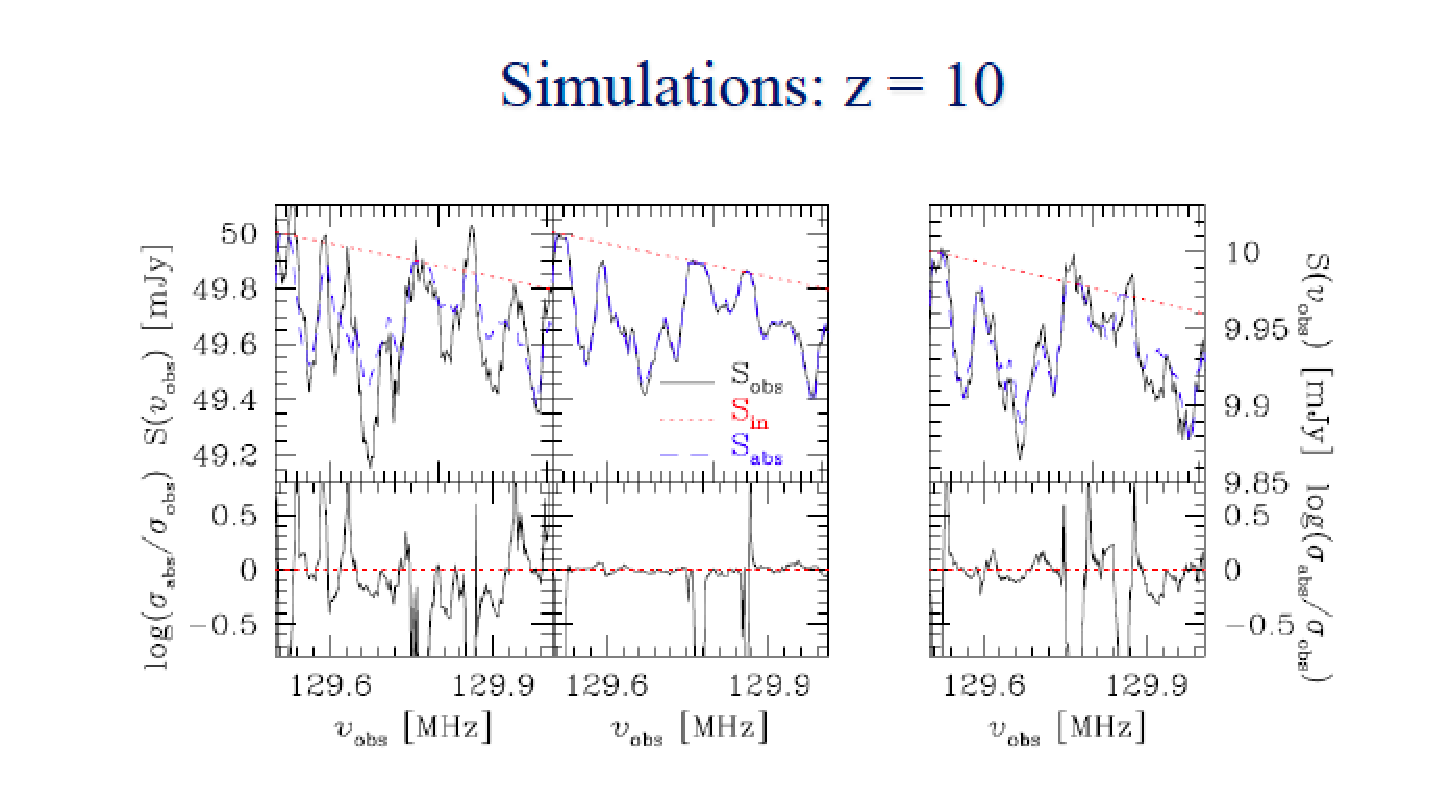
\includegraphics[scale=0.7]{EoR/c03/c03.s2.f11.eps}
   \caption{$z$=10$B$G$N7k2L!#(B$S_{{\rm in}}$$B$OEEGH8;K\Mh$N%9%Z%/%H%k$rI=$7$F$*$j!"(B$S_{{\rm abs}}$$B$O(B21cm$B5[<}@~$N%7%_%e%l!<%7%g%s7k2L$r!"(B$S_{{\rm obs}}$$B$O4QB,$K$h$k%N%$%:$b>h$;$?(B21cm$B5[<}@~$N7k2L$rI=$7$F$$$k!#$^$?!"(B$\sigma_{i}=S_{i}-S_{{\rm in}}$$B$G$"$k!#:8Fs$D$N%Q%M%k$OEEGH8;$N%U%i%C%/%9$,(B50mJy$B$N>l9g$G$N(BLOFAR$B$rA[Dj$7$?%N%$%:!J:8!K!"(BSKA1$B$rA[Dj$7$?%N%$%:!J1&!K$G$"$k!#$^$?!"1&$N%Q%M%k$O(BSKA1$B$rA[Dj$7$?$H$-$G%U%i%C%/%9$,(B10mJy$B$N>l9g$N7k2L$G$"$k!#(B$\Delta \nu=10{\rm kHz}$}
\label{fig:forest1}
\end{figure}
\begin{figure}[htbp]
   \centering 
   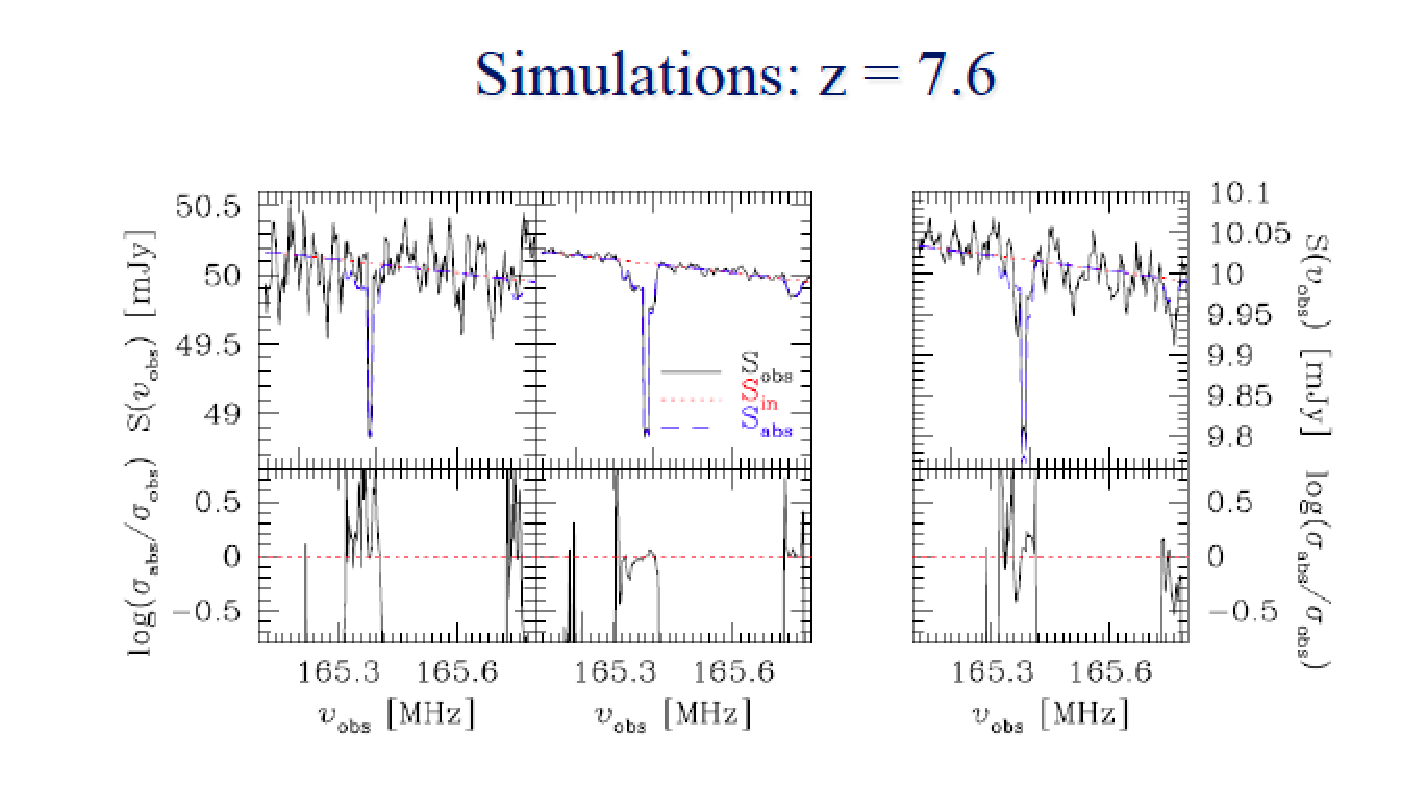
\includegraphics[scale=0.7]{EoR/c03/c03.s2.f12.eps}
   \caption{$z$=7.6$B$G$N%7%_%e%l!<%7%g%s7k2L!#@~$N@bL@$O!"?^(B\ref{fig:forest1}$B$N>l9g$HF1$8!#(B$\Delta \nu=5{\rm kHz}$}
\label{fig:forest2}
\end{figure}

\begin{figure}[htbp]
   \centering 
   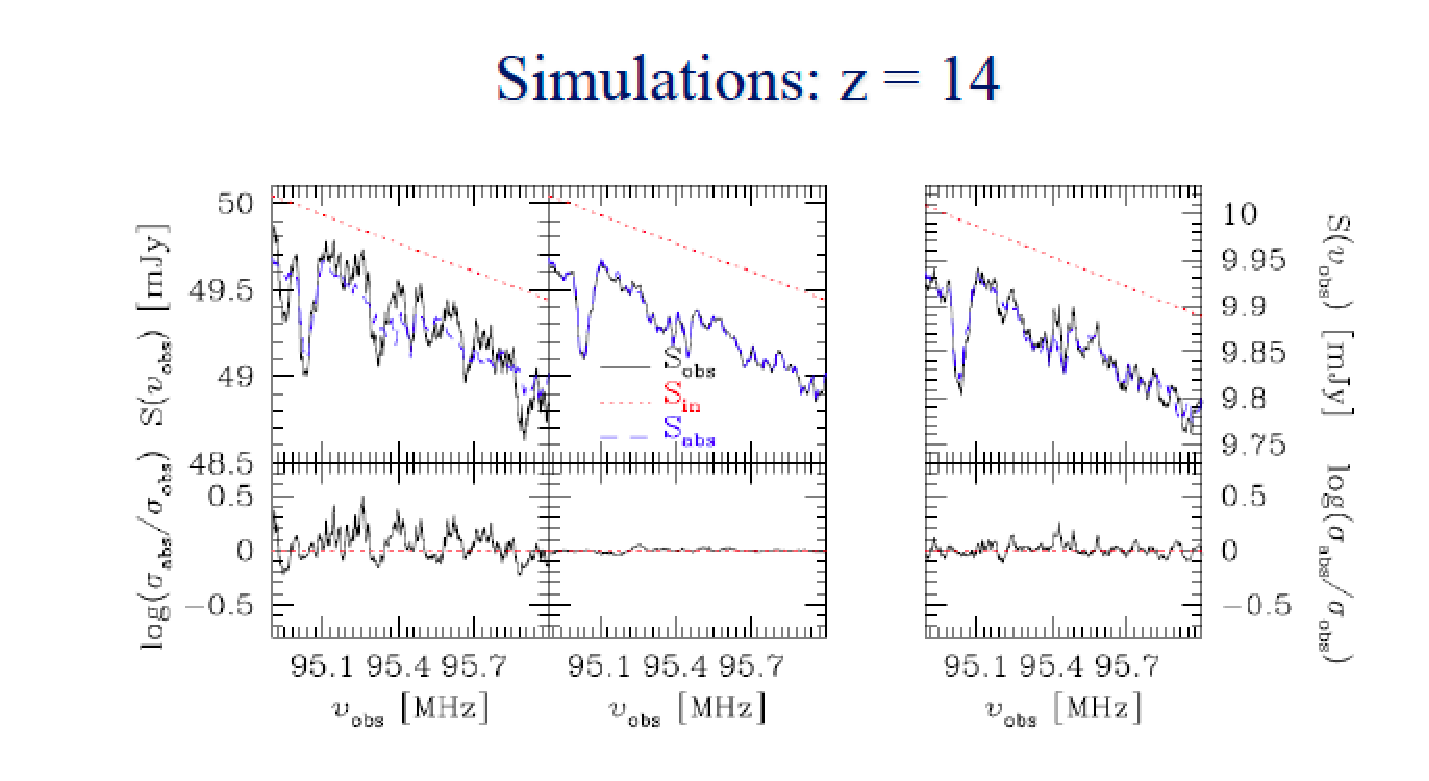
\includegraphics[scale=0.7]{EoR/c03/c03.s2.f13.eps}
   \caption{$z$=14$B$G$N%7%_%e%l!<%7%g%s7k2L!#@~$N@bL@$O!"?^(B\ref{fig:forest1}$B$N>l9g$HF1$8!#(B$\Delta \nu=20{\rm kHz}$}
\label{fig:forest3}
\end{figure}

\paragraph{$BMWLs$*$h$S5DO@(B}
\begin{itemize}
 \item $BGX7JE7BN8w$N5[<}@~$KCmL\$7$?(B21cm forest$B$O%H%b%0%i%U%#!<$d%Q%o!<%9%Z%/(B
$B%H%i%`$HAjJdE*$K:FEEN%4|$N$K$*$1$k6d2O4V%,%9$N29EY>uBV$J$I$N@-<A$rC5$k;v(B
$B$,=PMh$k!#(B
\item $B8=:_$N%7%_%e%l!<%7%g%s7k2L$@$H!"(BLOFAR$B$K$h$k4QB,$G$b5[<}@~$r8+$k;v$O2D(B
$BG=!#$?$@$7!"(B$\sim {\rm kHz}$$B$N?6F0?tJ,2rG=$,I,MW!#(B
\item $B6d2O4V%,%9$K$h$k5[<}$h$j$b!"%3%i%W%9$7$?E7BN$K$h$k5[<}$NJ}$,6/$$5[<}$r(B
$B0z$-5/$3$9!#(B
\item $B$=$b$=$bGX7JE7BN$,9b@VJ}JP0\$GB8:_$7$F$$$k;v$,I,MW>r7o$G$"$j!"8=:_!"(B
$z\sim 4$$B$G4QB,$5$l$F$$$kEEGH8;$N?tL)EY$r$h$j9b@VJ}JP0\$K30A^$7$FM=A[$5(B
$B$l$kA4E7$G$NEEGH8;$N?t$O(B$8\times 10^{2}-3\times 10^{4}$$B8DDxEY!J?^(B
\ref{fig:forest4}$B!K(B
 \citep{2002ApJ...577...22C,2009ApJ...704.1396X}$B!#(B 
\end{itemize}
\begin{figure}[htbp]
   \centering 
   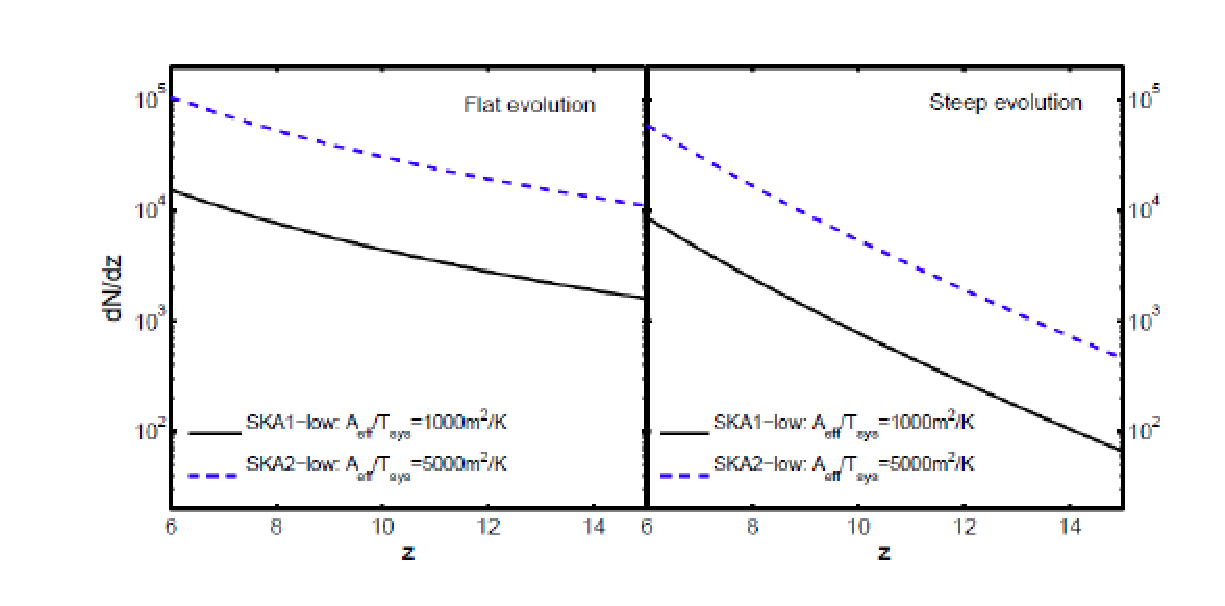
\includegraphics[scale=0.7]{EoR/c03/c03.s2.f14.eps}
   \caption{SKA1-low$B!J9u@~!K$H(BSKA2-low$B!J@DE@@~!K$G$NEEGH8;$N?tL)EY!JA4E7(B
 $B4QB,$7$?>l9g!K$NM}O@M=B,!#:8B&$O%/%'!<%5!<$N8D?t$N@VJ}JP0\?J2=$,$J$@$i(B
 $B$+$J>l9g$G!"1&B&$O9b@VJ}JP0\$G$O?tL)EY$,>.$5$$$,Dc@VJ}JP0\$K9T$/$KO"$l(B
 $B$F?tL)EY$,5^7c$K>e>:$9$k>l9g$rI=$7$F$$$k!#(B} 
\label{fig:forest4}
\end{figure}
%21cm forest
\subsection{HI$B%G!<%?$rMQ$$$?(BCD$B$H(BEoR$B$X$N@)8B(B}
\label{c03.s2.ss7}
SKA$B$G$O%Q%o!<%9%Z%/%H%k$rMQ$$$?2r@O$K$h$C$F!"E7BNJ*M}3X$d1'ChO@$NLdBj$K(B
$BBP$7$F2rEz$rM?$($k;v$,4|BT$5$l$F$$$k!#$=$NCf$G$b!"FC$K=EMW$JLd$$$H$7$F0J(B
$B2<$N$3$H$,5s$2$i$l$k!#(B 
\begin{itemize}
\item $B$$$D!"=iBe6d2O$,8=$l$?$N$+!)(B
\item $B=iBe6d2O$+$i$N;g308w$d(BX$B@~J|<M$N@-<A$O$I$N$h$&$J$b$N$J$N$+!)(B
\item IGM$B$N>.5,LO9=B$$O$I$&$J$C$F$$$k$N$+!)(B
\end{itemize}

\subsubsection{$BJ,;RNd5Q$5$l$?6d2O(B}
$B=iBe6d2O$O(B$z>$30$B$G!"%_%K%O%m!<$H8F$P$l$kHf3SE*<ANL$N>.$5$$%O%m!<(B
$B!J(B$M=10^{6-7}M_{\odot}$$B!KFb$G7A@.$5$l$k(B \citep{1996ApJ...464..523H,
2002ApJ...564...23B}$B!#$3$N;~4|$O<g$K(B${\rm H_{2}}$$BJ,;R$K$h$kNd5Q$,8z$/$,!"(B
$BNd5Q8zN($,0-$/!"%_%K%O%m!<Fb$G$N@17A@.$O0J2<$N%U%#!<%I%P%C%/8z2L$K$h$k1F(B
$B6A$r<u$1$k(B \citep{2000ApJ...534...11H, 2001ApJ...560..580R,
2006ApJ...648..835M}$B!#(B 
\begin{itemize}
\item $BD6?7@1GzH/$K$h$k%U%#!<%I%P%C%/(B
\item X$B@~2CG.(B
\item $B%$%*%s2=8w;RGX7J>l(B
\item ${\rm H}_{2}$$B2rN%J|<M(B
\end{itemize}
$B$^$?!"@17A@.$N8eH>$K$O(BLyman-Werner$BGX7J>l$,%_%K%O%m!<Fb$N@17A@.$rAK32$9$k!#(B
$B=iBe6d2O$O%U%#!<%I%P%C%/8z2L$K$h$C$F@17A@.$,AK32$5$l$k$?$a!"(B``$B@H$$(B''$B6d2O(B
$B$G$O$"$k$,!"=iBe6d2O$K$h$C$F(BCD$B$,Kk$r3+$1$k!#$3$N;~4|$r(B21cm$B@~$rDL$7$FC5$k(B
$BJ}K!$H$7$F$O!"(BWF$B%+%C%W%j%s%0;~4|$r8+$k$H$$$&$3$H$,5s$2$i$l$k!#@VJ}JP0\$N(B
$B4X?t$H$7$F(B21cm$B%Q%o!<%9%Z%/%H%k$r8+$?$H$-$K:G=i$KI=$l$k;3$HC+$r8+$k;v$K$h$C(B
$B$F!"=iBe6d2O7A@.$N;O$^$k;~4|$H4|4V$rC5$k;v$,$G$-$k$N$G$"$k!#(B($B?^(B\ref{KH4})
%\ref{bukuro.constraining.fig:fig1}) 

% \begin{figure}
% \centering
%  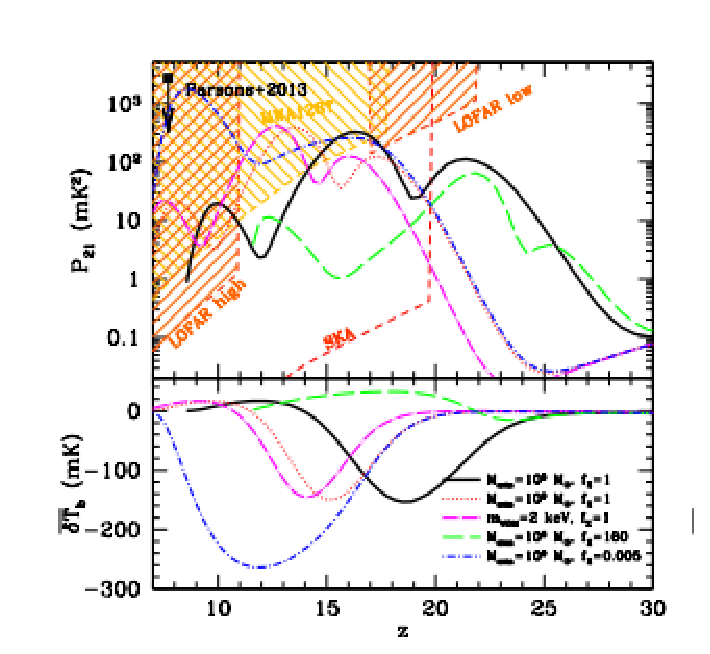
\includegraphics[width=0.5\hsize]{EoR/c03/c03.s2.f15.eps}
% \caption{(top)$z$$B$N4X?t$H$7$F8+$?;~$N(B21cm$B%Q%o!<%9%Z%/%H%k(B(fiducial model$B$O9u@~(B)$B$H(BMWA, LOFAR, SKA$B$N%N%$%:6J@~!#(B(bottom)$B51EY29EY$N(B$z$$B?J2=!#(B}
% \label{bukuro.constraining.fig:fig1}
% \end{figure}

\subsubsection{$B=i4|6d2O$N(BX$B@~J|<M$N@-<A(B}
$B=iBe6d2O$+$i$N(BX$B@~J|<M$O(BIGM$B$N29EY$r(BCMB$B29EY$h$j$b9b$$29EY$^$G>e>:$5$;$k$b(B
$B$N$H9M$($i$l$F$*$j!"(BIGM$B$N%$%*%s2=3d9g$,?t(B$\%$$BDxEY$N$H$-!"(BX$B@~J|<M$N%(%M%k(B
$B%.!<$N$[$H$s$I$,(BIGM$B$N2CG.$K$D$.9~$^$l$k!#(BX$B@~J|<M$O%$%*%s2=$h$j$b2CG.8;$H(B
$B$7$F8z2LE*$G$"$k!#$7$+$7!"4V@\E*$K$O$G$O$"$k$,!"(BX$B@~J|<M$K$h$C$F%8!<%s%:(B
$B<ANL$,>e$,$j!"8w;R2CG.$N%U%#!<%I%P%C%/$,CY$l$k$3$H$K$h$C$F:FEEN%$rCY$i$;(B
$B$k$H$$$&8z2L$b$"$k(B \citep{2013MNRAS.431..621M}$B!#(BX$B@~J|<M$H(BIGM$B$NAj8_:nMQ$O(B
$B$=$NBg$-$JJ?6Q<+M39TDx$K$h$C$FFCD'IU$1$i$l$k!J<0(B.\ref{eq:mfp}$B!K!#(B 
\begin{equation}
\lambda_{X}\sim 20 \overline{x}_{{\rm HI}}^{-1}\left(\frac{E_{X}}{300{\rm eV}}\right)^{2.6}\left(\frac{1+z}{10}\right)^{-1}c{\rm Mpc}
\label{eq:mfp}
\end{equation}
$\overline{x}_{{\rm HI}}$$B$OJ?6QCf@-?eAGN($G$"$j!"(B$E_{X}$$B$O8w;R$N%(%M%k%.!<(B
$B$G$"$k!#$3$N<0$h$j!"Fp(BX$B@~J|<M(B($E_{X}\le {\rm keV}$)$B$,(BIGM$B$HAj8_:nMQ$7!"(B
21cm$B@~$N8&5f$H7k$S$D$/;v$,J,$+$k!#(BIGM$B$N2CG.$K$h$k1F6A$O(B21cm$B%Q%o!<%9%Z%/(B
$B%H%k$N#2$DL\$N%T!<%/$KI=$l$k$,!"(BSKA1$B$G$O$3$N;~4|$N(B21cm$B%Q%o!<%9%Z%/%H%k$O(B
$B4QB,2DG=$HM=A[$5$l$F$$$k(B($B?^(B\ref{KH4})$B!#(B
%$B?^(B\ref{bukuro.constraining.fig:fig1}$B!K(B 

\subsubsection{$B2CG.4|$N(B21cm forest}
IGM$B$N29EY$,(BCMB$B29EY$h$j$b9b29$K2CG.$5$l$k0JA0$K$O!"9b@VJ}JP0\$NGX7JEEGH8;(B
$B$+$i$N8w$r(BIGM$B$,5[<}$9$k$3$H$K$h$j!"(B21 cm$B5[<}@~$,4QB,$5$l$k!#$3$l$r(B
Ly$\alpha$ forest$B$H$N%"%J%m%8!<$G(B21 cm forest$B$H8F$V!#(BSKA$B$G$b$3$N(B21 cm
forest$B$r4QB,$G$-$k$+$OFq$7$$$H$5$l$F$$$k(B \citep{2012MNRAS.425.2988M}$B!#:G(B
$BBg$NLdBj$H$7$F5s$2$i$l$k$N$OEEGH$r6/$/H/$9$k%/%'!<%5!<$J$I$NGX7JEEGH8;$,(B
$B9b@VJ}JP0\$G$bB8:_$9$k$+$H$$$&$3$H$G$"$k!#$7$+$7!"0E$$%/%'!<%5!<$G$bE}7W(B
$BE*<jK!$rMQ$$$l$P!"(B21cm forest$B$N8z2L$r2CG.4|A0$N(B21cm$B%Q%o!<%9%Z%/%H%k$N>.(B
$B%9%1!<%k$G8+$i$l$k2DG=@-$,$"$k(B \citep{2014MNRAS.441.2476E}$B!#(B21 cm$B%Q%o!<%9(B
$B%Z%/%H%k$NBg%9%1!<%k$O(BX$B@~$rJ|<M$9$k6d2O$K$h$k29EYMI$i$.$,;YG[E*$G$"$k$,!"(B
$B>.%9%1!<%k$G$O9b@VJ}JP0\$NEEGH$r6/$/H/$9$k(BAGN$B$J$I$,8z$$$F$/$k$N$G!"9b@V(B
$BJ}JP0\$N(BAGN$B$N<oB2$X$N@)8B$J$I$,4|BT$5$l$F$$$k!#(B 

\subsubsection{EoR$B%=!<%9(B}
EoR$B$N;~4|$d4|4V$NB>$K!"(B21cm$B%7%0%J%k$O(BEoR$B%=!<%9<+BN$K$D$$$F$b8@5Z$G$-$k!#(B
EoR$B$O8=:_$N4QB,$d>-Mh4QB,$N46EY8B3&$r2<2s$kbd>.6d2O$K$h$C$F0z$-5/$3$5$l(B
$B$k$H9M$($i$l$F$$$k$,!"$3$N$h$&$J9b@VJ}JP0\$Nbd>.6d2OFb$G$N@17A@.8zN($OITDj(B
$B@-$,Bg$-$/!"%U%#!<%I%P%C%/2aDx$b$h$/J,$+$C$F$$$J$$!#$7$+$7!"%U%#!<%I%P%C(B
$B%/8z2L$,@17A@.8zN($N?J2=$rD4@0$9$k$H9M$($i$l$F$*$j!"%U%#!<%I%P%C%/$NMM;R(B
$B$rCN$k;v$O(BEoR$B%=!<%9$rCN$k>e$G=EMW$G$"$k!#$3$l$rCN$k<j$,$+$j$N0l$D$H$7$F(B
EoR$B$N4v2?3XE*FCD'$r4QB,$9$k$H$$$&J}K!$,$"$k!#%$%*%s2=$r5/$3$7$F$$$k9=B$(B
$B$h$j$b>.%9%1!<%k$N(BEoR$B$N4v2?3XE*FCD'$r4QB,$9$k;v$K$h$j!"(BEoR $B%=!<%9$,$I$N(B
$B$h$&$K%O%m!<$H7k$S$D$-!"@17A@.8zN($K1F6A$rM?$($k$N$+$rCN$k;v$,$G$-$k$H9M(B
$B$($i$l$k!#(B 
%HIデータを用いたCDとEoRへの制限
\subsection{$B%P%j%*%s$H%@!<%/%^%?!<$NAjBPB.EY(B} 
\label{c03.s2.ss8}

$B1'Ch$N@2$l>e$,$j0J9_$N%P%j%*%s$NL)EY$f$i$.$N;~4VH/E8$dG.;K$O!"=iBeE7BN(B
$B!J=iBe@1!&=iBe6d2O!K7A@.2aDx$K$*$$$F=EMW$JLr3d$r2L$?$9!#FC$K!"=iBeE7BN$+(B
$B$i$NmU<M$O!"1'Ch$N:FEEN%$r5/$3$71'Ch0E9u;~Be$d$=$N8e$NE7BN7A@.$KBg$-$J1F(B
$B6A$rM?$($k$?$a!"1'Ch@2$l>e$,$j0J9_$N9=B$7A@.$rM}O@E*$KM}2r$9$k$3$H$O6K$a(B
$B$F=EMW$G$"$k!#(B

$B6aG/!"1'Ch@2$l>e$,$j0J9_$K$*$1$k%P%j%*%s$H%@!<%/%^%?!<$NAjBPB.EY$,9=B$7A(B
$B@.$dE7BN7A@.$KM?$($k1F6A$,(B\citet{2010PhRvD..82h3520T}$B$K$h$C$F;XE&$5$lCmL\(B
$B$r=8$a$F$$$k!#E57?E*$JAjBPB.EY$OFs>hJ?6Q$G(B30km/s$BDxEY$H$J$j!"@2$l>e$,$jD>(B
$B8e$N2;B.(B(6km/s)$B$rBg$-$/>e2s$kD62;B.$JAjBPB.EY$,IaJWE*$KB8:_$9$k!#$3$l$^$G(B
$B$NM}O@E*$J8&5f$G$O!"%P%j%*%s$H%@!<%/%^%?!<$NAjBPB.EY$K$h$k9=B$7A@.$KBP$9(B
$B$k1F6A$O#2<!$N8z2L$G$"$j!"$"$^$jCmL\$5$l$FMh$J$+$C$?$,!"%P%j%*%s$H%@!<%/(B
$B%^%?!<$K$3$N$h$&$JBg$-$JAjBPB.EY$,B8:_$9$k>u67$G$O!"=i4|$KAjBPB.EY$,$J$$(B
$B>l9g$HHf3S$7$F%@!<%/%^%?!<%O%m!<$N?tL)EY$d$=$NFbIt$N%P%j%*%s%U%i%/%7%g%s(B
$B$,>.$5$/$J$k$3$H$,(B\citet{2012ApJ...747..128N, 2013ApJ...763...27N}$B$N8&5f(B
$B$GL@$i$+$H$J$j!"%P%j%*%s$H%@!<%/%^%?!<$NAjBPB.EY$K$h$kE7BN7A@.$KBP$9$k1F(B
$B6A$K$D$$$F$N8&5f$,(B2010$BG/0J9_$K@9$s$K$J$C$F$-$F$$$k!#(B


$B%P%j%*%s$H%@!<%/%^%?!<$NAjBPB.EY$K$h$C$F1F6A$r<u$1$k%@!<%/%^%?!<%O%m!<$N(B
$B<ANL%9%1!<%k$O$=$N;~!9$N(BJeans$BD9$d(BJeans$B<ANL$N;~4VJ?6Q$KAjEv$9$k(B
filtering mass$B$N%9%1!<%k$G$"$j!"6qBNE*$K$O<g$K(B$10^5M_{\odot}$$B!A(B
$10^7M_{\odot}$$B$N%@!<%/%^%?!<%O%m!<$N7A@.$K1F6A$,=P$k!#$3$N%9%1!<%k$N%@!<(B
$B%/%^%?!<%O%m!<$O=iBe@1$d=iBe6d2O$KBP1~$7!"AjBPB.EY$N%3%R!<%l%s%9%9%1!<%k(B
$B$O%P%j%*%s2;6A?6F0$N%9%1!<%k(B($108h^{-1}$Mpc)$B$H$[$\F1$8$G$"$k$?$a!"1'Ch:F(B
$BEEN%4|$*$1$kE7BN7A@.$d:FEEN%$=$N$b$N$KBP$7$FBg$-$J%$%s%Q%/%H$rM?$($k$HM=(B
$BA[$5$l!"I,A3E*$K(BSKA$B$K$h$kCf@-?eAG(B21cm$B@~$N4QB,$,%P%j%*%s$H%@!<%/%^%?!<$NAj(B
$BBPB.EY$,E7BN7A@.$K5Z$\$91F6A$K$D$$$F$NCN8+$rF@$k6/NO$J<jCJ$H$J$k!#(B

$B1'ChO@E*$J9=B$7A@.$N?tCM%7%_%e%l!<%7%g%s$rMQ$$$F!"%P%j%*%s$H%@!<%/%^%?!<(B
$B$NAjBPB.EY$,:FEEN%4|$NE7BN7A@.$K5Z$\$91F6A$rD4$Y$k8&5f$,J#?t$N8&5f%0%k!<(B
$B%W$G9T$o$l$F$$$k(B
\citep{2011MNRAS.412L..40M,2012ApJ...747..128N,2013ApJ...763...27N}$B!#?^(B
\ref{c6.s3.ss5.f1}$B$O@VJ}JP0\(B$23$$B$H(B$19$$B$K$*$$$F7A@.$5$l$?%,%9%/%i%&%I$N<ANL4X(B
$B?t$r<($7$?$b$N$G!"B.EY:9$N1F6A$H$7$F%,%9%/%i%&%I$N<ANL$H?tL)EY$,2<$,$k79(B
$B8~$,L@3N$K$o$+$k!#B.EY:9$,(B$60$ km/s$B$N>l9g$N%,%9%/%i%&%I$N<ANL4X?t$O!"(B
$\sigma_8$$B$r(B$0.9$$B$+$i(B$0.8$$B$K2<$2$?>l9g$HF1DxEY$N1F6A$,$"$k!#;~4V$,7P$D$H!"B.(B
$BEY:9$,>.$5$/$J$k$?$a$KB.EY:9$NM-L5$K$h$k<ANL4X?t$X$N1F6A$O>.$5$/$J$k798~(B
$B$,8+$i$l$k!#@VJ}JP0\(B$19$$B$K$*$$$F$O!"B.EY:9$NM-L5$K$h$C$F<ANL4X?t$K(B2$BG\DxEY$N(B
$B0c$$$,8+$i$l$?$,!"@VJ}JP0\(B$10$$B$G$OB.EY:9$NM-L5$K$h$k<ANL4X?t$X$N1F6A$O$h$j(B
$B8BDjE*$H$J$j(B$10$\%$BDxEY$H$J$k!#$^$?!"0lC6%,%9%/%i%&%IFb$G$N@17A@.$,;O$^$k$H!"(B
$BAjBPB.EY$N1F6A$O7A@.$5$l$k=iBeE7BN$N7A@.N(!&EEN%8w;R$K$h$k:FEEN%!&=E85AG(B
$B6!5k$J$I$KGH5Z$9$k!#AjBPB.EY$NBg$-$JNN0h$G$O!"@17A@.N($N?d0\$,B>$NNN0h$h(B
$B$j$bCY1d$7!"$=$l$KH<$C$F:FEEN%$d=E85AG6!5k$bCY1d$9$k(B($B?^(B
\ref{c6.s3.ss5.f2})$B!#$3$N7k2L!"AjBPB.EY>l$N%3%R!<%l%s%9%9%1!<%k$GEEN%EY$N(B
$B6u4VE*JQF0$,H/@8$7!"(B21 cm$B@~J|<M$N6u4VJ,I[$N%Q%o!<%9%Z%/%H%k$KH?1G$5$l$k$H(B
$BM=A[$5$l$k!#(B

\begin{figure}[!t]
 \centering \includegraphics[width=0.9\linewidth] {EoR/c03/c03.s2.f16.eps}
 \caption{$B@VJ}JP0\(B23($B>eCJ(B)$B$H(B19($B2<CJ(B)$B$K$*$1$k%,%91@$N<ANL4X?t!#:8$H1&$O$=(B
 $B$l$>$l(Bdifferential$B$J<ANL4X?t$H(Bcumulative$B$J<ANL4X?t!#(B
 \label{c6.s3.ss5.f1}}
\end{figure}
\begin{figure}[!h]
 \centering \includegraphics[width=10cm] {EoR/c03/c03.s2.f17.eps}
 \caption{$B>eCJ!'%P%j%*%s$H%@!<%/%^%?!<$NAjBPB.EY$NBP$9$k(BPop-III$B$HA4BN$N@1(B
 $B7A;K$N;~4VH/E8!#2<CJ!'(BPop-III$B$N7A@.N($NA4BN$N@17A@.N($KBP$9$k4sM?$N;~4VH/E8!#(B
 \label{c6.s3.ss5.f2}}
\end{figure}


SKA$B$N4QB,7k2L$r@5$7$/2r<a$9$k$K$O!"%P%j%*%s$H%@!<%/%^%?!<$NAjBPB.EY$K$h$k(B
$B9=B$7A@.$X$N1F6A$rDjNLE*$K8+@Q$b$k$3$H$,I,MW$G$"$k!#@VJ}JP0\$,(B$20$$B0J>e$N@1(B
$B7A@.3hF0$,;O$^$C$F$$$J$$;~4|$N4QB,$K$O!"%,%9%/%i%&%I$KK-IY$K4^$^$l$k(B
H$_2$$B$d(BHD$B$H$$$C$?J,;R$N2sE>A+0\J|<M$,%,%9$NJ,I[$NNI$$%H%l!<%5!<$H$J$k!#(B
H$_2$$B$N(B$J=2\rightarrow 0$$B$N2sE>A+0\!"(BHD$B$N(B$J=4\rightarrow 3$$B$N2sE>A+0\$,=P(B
$B$9(B$533$ GHz$B$NJ|<M$O@VJ}JP0\(B$35\sim 40$$B$G$"$l$P!"(B$14$ GHz$B$^$G4QB,$G$-$k(BPhase-1$B$N(B
SKA-MID $B$G4QB,2DG=$G$"$k!#99$K(B $24$ GHz$B$^$G4QB,2DG=$G$"$k(BPhase-2$B$G$"$l$P!"@V(B
$BJ}JP0\(B$20$$BDxEY$^$G4QB,2DG=$G$"$k!#$^$?!"=iBeE7BN$,7A@.$5$l1'Ch:FEEN%$,?J$`(B
$B2aDx$G$N%P%j%*%s$H%@!<%/%^%?!<$NAjBPB.EY$N1F6A$r4QB,$9$k$K$O!"Cf@-?eAG$N(B
21 cm$B@~$r%H%l!<%5!<$H$7$F@VJ}JP0\(B$6<z<20$$B$NCf@-?eAG$+$i$NJ|<M$r(B$50 \sim 350$
MHz
$B$N<~GH?tBS$r%+%P!<$9$k(BSKA-low$B$,:GE,$G$"$k!#(B

%バリオンとダークマターの相対速度
\subsection{EoR/Cosmic Dawn$B4|$N1'ChO@(B}
\label{c03.s2.ss9}

$B6aG/!"(BWMAP, Planck$B$r$O$8$a$H$9$k1'Ch%^%$%/%mGHGX7JmU<M(B(CMB)$B29EYMI$i$.$dJP(B
$B8w$N4QB,!"$^$?(BSDSS$B$r$O$8$a$H$9$kBg5,LO6d2O%5!<%Y%$$K$h$k!"1'Ch$N9=@.MWAG(B
$B$dMI$i$.$N=i4|>r7o$rM?$($k%$%s%U%l!<%7%g%sM}O@$r5-=R$9$k1'ChO@%Q%i%a!<%?(B
$B$N@:L)B,Dj$,2DG=$H$J$j!"1'ChO@$O@:L)2J3X$H$7$F3NN)$5$l$F$-$F$$$k!#(B

$B$7$+$7$^$@$^$@!"%@!<%/%^%?!<!"%@!<%/%(%M%k%.!<$N@5BN$d%K%e!<%H%j%N<ANL$J(B
$B$I2r7h$9$Y$-LdBj$,B8:_$9$k!#>-Mh4QB,$K$*$1$k$3$l$i$NLdBj2r7h$KBP$9$k%"%W(B
$B%m!<%A$H$7$F$O!"C1=c$K$O;~4V!"6u4VE*$K$h$jI}9-$$4QB,$r9T$&$3$H$G$"$k!#(B

SKA$B$O!"0J>e$N$h$&$J8=:_$N1'ChO@$K$*$1$kLdBj2r7h$K$H$C$FHs>o$K=EMW$J0LCV$r(B
$B@j$a$F$$$k!#$3$l$^$G4QB,$7$?$3$H$N$J$$!";~4VE*$K$O9b@VJ}JP0\1'Ch$N>pJs$r(B
$BM?$($F$/$l$k$@$m$&$7!"6u4VE*$K$O$h$j>.$5$J%9%1!<%k$^$G4QB,$G$-$k$+$i$G$"(B
$B$k!#(B

\paragraph{$BL)EYMI$i$.$N>pJs$rMQ$$$?1'ChO@%Q%i%a!<%?$X$N@)8B(B}

SKA$B$O!"(B21cm$B51EY29EY!J(B21cm$B%7%0%J%k!K$rL)EY>l$NDI@W;R!J%H%l!<%5!<!K$H$7$F;H$$!"(B
$B1'ChO@%Q%i%a!<%?$KBP$7$F@)8B$rM?$($k$3$H$,=PMh$k!#(B

$B$3$N51EY29EY$O!"%9%T%s29EY!"Cf@-?eAG$N3d9g$HL)EY>l$K0MB8$9$k!#(B
$BFC$K%9%T%s29EY$,(BCMB$B29EY$KHf$Y$FHs>o$K9b$$>l9g!"(BCMB$B29EY$+$i$_$?51EY29EY$O!"(B
$B$*$*$h$=(B
\begin{equation}
\delta T_B = (1 + \delta ) x_H \times \cdots
\end{equation}
$B$H=q$1$k!#(B$x_H$$B$,Cf@-?eAG$N3d9g$G!"(B$\delta$$B$,J*<A$NL)EY>l$rI=(B
$B$9(B~\citep{2006PhR...433..181F}$B!#FC$K(B$x_H = 1$$B$N>l9g$K$O(B$\delta T_B$$B$O!"L)(B
$BEY>l$NL5%P%$%"%9DI@W;R$H$J$k!#$3$N$h$&$JHs>o$KM}A[2=$5$l$?>u67$G$N%Q%i%a!<(B
$B%?7hDj@:EY$O!"(BSKA0 (SKA1$B$NH>J,$N%"%s%F%J$N?t(B)$B$G(B$z=7,7.5,8$$B$G$N51EY29EY$r(B
$B4QB,$7$?>l9g!"(BPlanck$B$H$[$\F1DxEY!"(BSKA2(SKA1$B$N#4G\$N%"%s%F%J$N?t(B)$B$G$O!"FC(B
$B$K>.%9%1!<%k$N>pJs$r$h$j@:L)$KB,Dj$9$k$3$H$,2DG=$H$J$k$N$G!"Nc$($P=i4|MI(B
$B$i$.%Q%o!<%9%Z%/%H%k$N%9%Z%/%H%k;X?t$NJQ2=(B(running spectral index)$B$d%K%e!<(B
$B%H%j%N<ANL$N7hDj@:EY$,(BPlanck$B$KHf$Y%U%!%/%?!<#3DxEY2~A1$9(B
$B$k(B~\citep{2008PhRvD..78f5009P,2009PhLB..673..173B, 2011JCAP...02..021A}$B!#(B

\paragraph{$B!V1'ChO@E*MWAG!W$H!V1'ChJ*M}E*MWAG!W$NJ,N%(B}

$B$7$+$7<B:]$K$O!"$3$N$h$&$JM}A[E*$J>u67$K$O$J$C$F$*$i$:!"4QB,$5$l$k@VJ}JP(B
$B0\$G$N%,%929EY$J$I$5$^$6$^$J1'ChJ*M}E*$JMWAG$,(B$\delta T_B$$B$K$O:.F~$7$F$/(B
$B$k!#1'ChO@$H$3$N1'ChJ*M}E*$JMWAG$r40A4$KJ,N%$9$k$?$a$K$O!"1'ChJ*M}E*8z2L(B
$B$KBP$9$kM}O@%b%G%k$N9=C[$,$^$:9M$($i$l$k(B~\citep{2008PhRvD..78b3529M}$B!#$b$&(B
$B$R$H$D$O!"(B$\delta T_B$$B$N%Q%o!<%9%Z%/%H%k$K$*$1$k@VJ}JP0\OD$_$rMQ$$$k$3$H(B
$B$G$"$k!#$3$N@VJ}JP0\OD$_$O!"%I%C%W%i!<%7%U%H$K5/0x$9$k$,4QB,E*$K$O%Q%o!<(B
$B%9%Z%/%H%k$r3QEY0MB8@-$GE83+$7$?:]$K9b<!%b!<%a%s%H$H$7$FM?$($i$l$k!#FC$K(B
$B%X%-%5%G%+%]!<%k$O1'ChJ*M}E*8z2L$,F~$i$J$$L)EY>l$N$h$$DI@W;R$H$7$F9M$($i(B
$B$l!"$3$N9b<!%b!<%a%s%H$N4QB,$b=EMW$H9M$($i$l$k(B~\citep{2006ApJ...653..815M,2008PhRvD..78b3529M}$B!#(B

\paragraph{$B6d2O4V%,%929EY$N>pJs$rMQ$$$??7J*M}$NC5::(B}

$BL)EY>l$NDI@W;R$H$7$F>e$G$O(B21cm$B%7%0%J%k$r9M$($F$-$?$,!"@h$K$b=R$Y$?$h$&$K(B
21 cm$B%7%0%J%k$O!"1'Ch$N%$%*%s2=N($d6d2O4V%,%9(B(inter galactic medium
(IGM))$B$N29EY$K$b0MB8$9$k!#I8=`1'Ch%b%G%k$K$*$1$k9=B$7A@.%7%J%j%*$K4p$E$$(B
$B$?!"%$%*%s2=N($d(BIGM$B$N>uBV$N;~4VJQ2=$K2C$($F!"$5$i$K$3$l$i$N?J2=$,JQ99$r<u(B
$B$1$k$h$&$J?7$?$J%7%J%j%*$,$"$l$P!"(B21 cm$B%7%0%J%k$N4QB,$O9b@VJ}JP0\1'Ch$K$*(B
$B$1$k?7$?$JJ*M}$X$N@)8B$rM?$($k$b$N$H$7$F=EMW$G$"$k!#(B

$B$^$:$=$N$h$&$J8uJd$H$7$F!"0E9uJ*<A$N@-<A$,>e$2$i$l$k!#I8=`E*$JNd$?$$0E9u(B
$BJ*<A!J(BCDM$B!K%b%G%k$H$O0[$J$j!"<ANL$,Hf3SE*7Z$$$h$&$J$$$o$f$kCH$+$$0E9uJ*<A(B
 (Warm Dark Matter(WDM)) $B$,$7$P$7$P5DO@$5$l$F$$$k!#$3$N(BWDM$B%b%G%k$G$O!">.%9(B
$B%1!<%k9=B$$N7A@.$,M^@)$5$l!"6d2O7A@.$,I8=`E*$JNd$?$$0E9uJ*<A$N>l9g$h$jCY(B
$B$/$J$k!#7k2L$H$7$F!"(B21 cm$B%7%0%J%k$K$*$$$F!"1'ChJ*M}E*MWAG$,1F6A$rM?$($k;~(B
$B4|$,JQ99$r<u$1$k$N$G4QB,$+$i$3$N(BWDM$B%7%J%j%*$K@)8B$rM?$($k$3$H$,$G$-$k$H4|(B
$BBT$5$l$k(B~\citep{2014MNRAS.438.2664S}$B!#(B


$B$^$?0E9uJ*<A$NBP>CLG$dJx2u$r9M$($k$H!"$=$l$O(BIGM$B$rCH$a$k8z2L$H$7$FF/$-!"(B
IGM$B29EY$N;~4V?J2=$NMM;R$,I8=`%b%G%k$H$O0[$J$C$F$/$k!#$3$N$h$&$J(BIGM$B29EY$N(B
$B;~4VJQ2=$rDL$8$??7$?$J%b%G%k$X$N@)8B$K$H$C$F$b(B21cm$B%7%0%J%k$OM-8z$G$"(B
$B$k(B~\citep{2014JCAP...11..024E}$B!#(B

$BB>$K$b!"=i4|<'>l$d!"86;O%V%i%C%/%[!<%k$J$I$N!VJQ$o$C$?FC@-$r;}$C$?J*<A!W(B
$B$KBP$9$k@)8B$H$7$F$b(BSKA$B$K$h$k(B21cm$B4QB,$O=EMW$G$"$k$H9M$($i$l(B
$B$k(B~\citep{2014PhRvD..89j3522S}$B!#(B 

\paragraph{$B%P%k%/%U%m!<(B}

$B>\:Y$O(B``Bulk flows and the end of dark ages''$B$G?($l$k$,!"(Bbaryon$B$H0E9uJ*<A(B
$B$N4V$NB.EY>l$N0c$$$,9=B$7A@.$K1F6A$rM?$($k$3$H$,!";XE&$5$l$F$$(B
$B$k(B~\citep{2010PhRvD..82h3520T}$B!#$3$NAjBPB.EY$N1F6A$H$7$F$O!">.%9%1!<%k$N9=(B
$BB$7A@.$NM^@)$J$I$,9M$($i$l$k!#$3$N8z2L$O!"(B21 cm$B%7%0%J%k$GC5$k9b@VJ}JP0\1'(B
$BCh$G82Cx$G$"$k$N$G!"(BSKA$B$GC5$k?7$?$J1'ChO@E*8z2L$H$7$F5DO@$5$l$F$$$k!#(B


\paragraph{$B$=$NB>(B}

\begin{itemize}

\item $B=i4|Hs%,%&%9@-(B

$B=i4|6JN(MI$i$.$NE}7WJ,I[$O!"MI$i$.$N<o$H$J$k%9%+%i!<>l$NAj8_:nMQ$d>l$NMI$i$.$r6JN(MI$i$.$X$HE>49$9$k:]$NHs@~7A8z2L$K$h$j%,%&%9J,I[$+$i$o$:$+$K$:$l$k2DG=@-$,$"$k$3$H$,;XE&$5$l$F$$$k!#$3$N$h$&$J>l9g!"Hs>o$KBg$-$J%9%1!<%k$G$N6d2OJ,I[$,1F6A$r<u$1$F(B
$B%,%&%9J,I[$N;~$H$O0[$J$k%Q%o!<%9%Z%/%H%k$N?6$kIq$$$,8+$i$l$k!#1'Ch:FEEN%4|$N(B21cm$B%7%0%J%k$K$O!"(B
$B%$%*%s2=N($N>pJs$,F~$C$F$$$k$,!"$3$N%$%*%s2=N($,6u4VJ,I[$7$F$$$k>l9g!"(B21cm$B51EY29EY$N%Q%o!<%9%Z%/%H%k$O!"$=$NJ,I[$K0MB8$9$k!#6d2OJ,I[$HF1$8$h$&$K!"$3$N%$%*%s2=N($NJ,I[$K$b=i4|MI$i$.$NHs%,%&%9@-$O1F6A$rM?$($k$N$G!"(BSKA$B$J$I$K$h$j=i4|MI$i$.$NHs%,%&%9@-$K@)8B$rM?$($k$3$H$,=PMh$k!#(B
Planck$B$K$h$k(BCMB$B4QB,$GF@$i$l$F$$$k$3$NHs%,%&%9@-$KBP$9$k@)8B$HF1DxEY$N@)8B$rM?$($k$H4|BT$5$l$F$$$k(B~\citep{2011PhRvL.107m1304J}$B!#(B


\item $B1'ChO@E*=ENO%l%s%:8z2L(B

$B9b@VJ}JP0\$GH/$;$i$l$?(B21cm$B%7%0%J%k$O2f!9$KFO$/$^$G$K1'ChBg5,LO9=B$$rDL2a$7$F$/$k$N$G$=$N=ENO>l$N1F6A$K$h$C$F%l%s%:8z2L$r<u$1$k!#$3$N%l%s%:8z2L$rCj=P$G$-$l$P!"$"$i$?$J1'ChBg5,LO9=B$$N(Bprobe$B$H$7$F4|BT$G$-$k!#(BSKA$B$G$O==J,B,Dj2DG=$G$"$k$H9M$($i$l$F$$$k(B~\citep{2006ApJ...653..922Z,2006astro.ph.11862B}$B!#(B

\end{itemize}

\paragraph{$B$^$H$a(B}

SKA$B!J(BSKA-Low$B!K$O!"@VJ}JP0\$r<u$1$?Cf@-?eAG$N(B21cm$B@~%7%0%J%k$rB*$($k$3$H$G(B
$z = 6 - 27$$B$H$$$&9b@VJ}JP0\1'Ch$N;Q$rL@$i$+$K$9$k$H4|BT$5$l$F$$$k!#$3$N4QB,$K$h$j!"$3$l$^$G$N1'ChO@%Q%i%a!<%?$N7hDj@:EY$,8~>e$9$k$@$1$G$J$/!"0E9uJ*<A$N@-<A$J$I?7$?$JJ*M}$K4QB,E*$KGw$k$3$H$,$G$-$k$H4|BT$5$l$F$$$k!#(B


%Cosmology from EoR/Cosmic Dawn
\subsection{$B1'ChO@E*4QB,$HCf@-?eAG(B21~cm$B@~$NAj8_Aj4X(B}%\label{c6.s2}
\label{c03.s2.ss10}

SKA$B7W2h$K$*$$$F!"(BCosmic Dawn~(CD)$B$d(BEpoch of Reionization~(EoR)$B5/8;$N1'Ch(B
$BO@E*$JCf@-?eAG(B21~cm$B@~$N8!=P$O=EMW$J%-!<%5%$%(%s%9$N0l$D$G$"$k!#$7$+$7$J$,(B
$B$i!"$=$N4QB,GHD9BS$OE7$N@n6d2O$d6aK56d2O$K$"$k6/$$EEGH8;!"CO5e$NEEN%AX$N(B
$B1F6A!"$=$7$F%i%8%*GH$N43>D$J$I$K$h$j7h$7$FM}A[E*$J4QB,>r7o$H$O8@$($J$$!#(B
$B$9$J$o$A!"1'ChO@E*(B21~cm$B$N%7%0%J%k$O$3$l$i(B''$B%N%$%:(B''$B$KKd$b$l$F$7$^$$!"$=$N(B
$B8!=P$O:$Fq$r6K$a$k!#$3$N$h$&$J:$Fq$5$r2sHr$9$kJ}K!$N0l$D$H$7$F!"B>$N4QB,(B
$B$H$NAj8_Aj4X$,5s$2$i$l$k!#Fs$D$NFHN)$J4QB,!J$b$7$/$OGHD9!K$NAj8_Aj4X$r$H(B
$B$l$P!"$=$l$>$l$N%7%9%F%^%F%#%C%/$J%N%$%:$O$*8_$$BG$A>C$79g$$!"%N%$%:$KKd(B
$B$b$l$F$$$?%7%0%J%k$N8!=P$,2DG=$H$J$k!#(B

CD$B$d(BEoR$B5/8;$N%7%0%J%k$r<h$j=P$9;v$rL\E*$H$7$?;~!"1'ChO@E*(B21~cm$B@~$HAj8_Aj(B
$B4X$r<h$kM-NO$J4QB,$H$7$F!"1'Ch%^%$%/%mGHGX7JJ|<M(B~(CMB)$B!"9b@VJ}JP0\$N6d2O(B
$BC5::!"$=$7$F!"6a@V30@~GX7JJ|<M(B~(NIRB)$B$,5s$2$i$l$k!#$3$N>O$G$O!"$3$l$i$N4Q(B
$BB,$H(BCD$B$d(BEoR$B$H$N4XO"@-!"$=$7$F!"1'ChO@E*(B21~cm$B@~$HAj8_Aj4X$r$H$k;v$K$h$C$F!"(B
$B$I$N$h$&$J(BCD$B$d(BEoR$B$K4X$9$k>pJs$K%"%/%;%9=PMh$k$+$K$D$$$F%l%S%e!<$r$9$k!#(B

	
\subsubsection{CMB$B$H$NAj8_Aj4X(B}

CMB$B29EY$f$i$.$N@:L)4QB,$K$h$j!"2f!9$O1'Ch$NMM!9$J>pJs$K%"%/%;%9$G$-$k!#(B
$B$=$l$O!"1'Ch:F%$%*%s2=%W%m%;%9$bNc30$G$O$J$$!#(BCMB$B8w;R$O!"<+M3EE;R$H$N;6Mp$N:]!"(B
$B%I%C%W%i!<%7%U%H$r<u$1$k(B~\citep{zeldovich}$B!#(B
EoR$B4|$K$O<+M3EE;R?t$,G|Bg$KA}$($k$?$a!"$3(B
$B$N%I%C%W%i!<%7%U%H$,(BEoR$B4|5/8;$N29EY$f$i$.$,@8$8$k%a%+%K%:%`$H$J$k!#(B
$B$3$N;v$+$i!"(BCMB$B$N29EY$f$i$.$K$O!"(BEoR$B4|$N<+M3EE;R$N?tL)EY(B($B%$%*%s2=EY$b4^$`(B)$B$H$=$N!JG.1?F0$b$7$/$O%P%k%/1?F0$N!KB.EY$N?J2=;K$,Kd$a9~$^$l$F$$$k$H8@$($k!#(B
$BBg$^$+$K8@$($P!"Bg%9%1!<%k$N29EY$f$i$.$K$O1'ChJ?6Q$N%$%*%s2=EY$,!">.%9%1!<(B
$B%k$G$O%$%*%s2=%P%V%k$K$h$C$F:n$i$l$k6I=jE*$J%$%*%s2=EY$,$=$l$>$lL)@\$K4X(B
$B$o$C$F$/$k(B ($B>\$7$$%l%S%e!<$H$7$F!"Nc$($P(B~\cite{2008RPPh...71f6902A}
$B$r8+$h(B)$B!#(B

$B$7$+$7$J$,$i!"(BEoR$B4|$K@8@.$5$l$k29EY$f$i$.$O29EY$f$i$.A4BN$G8@$($P>.$5$/!"(B
$BB>$N5/8;$N29EY$f$i$.$N@.J,$KKd$b$l$F$$$k!#$3$NKd$b$l$?%7%0%J%k$rIb$+$S>e$,$i$;(B
$B$kJ}K!$N0l$D$,!"(B21~cm$B@~$H(BCMB$B$NAj8_Aj4X$G$"$k!#$7$?$,$C$F!"3F!9$N<+8JAj4X$G$OKd$b$l(B
$B$F$7$^$C$F$$$k(BEoR$B$N>pJs$K%"%/%;%9$G$-$k2DG=@-$b$"$k$3$H$+$i!"$3$NAj8_Aj(B
$B4X$NJ*M}$NM}2r$N$?$a$K!"2r@OE*!"?tCM7W;;E*$NN>J}$NLL$+$iB?$/$N8&5f$,$J$5(B
$B$l$F$$(B
$B$k(B~\citep{2005MNRAS.360.1063S,2008MNRAS.384..291A,2004PhRvD..70f3509C,2006ApJ...647..840A,2007MNRAS.377..168S,2010MNRAS.402.2617T,2010MNRAS.402.2279J,2011MNRAS.414.3424T}$B!#(B
$B$=$N7k2L!"Bg$-$J%9%1!<%k$G$NAj8_Aj4X%7%0%J%k$NBg$-$5$O!"1'ChJ?6QE*$J(B
$B%$%*%s2=$N%9%T!<%I$K0MB8$9$k$3$H$,<($5$l$?!#%$%*%s2=$,5^7c$K?J$`$[$I!"$=$N(B
$B%7%0%J%k$NBg$-$5$OBg$-$/$J$k$N$G$"$k!#?^(B~\ref{fig:cmb_cross}$B$O(B~\cite{2010MNRAS.402.2617T} $B$K4p$E$$$F!":F%$%*%s2=%b%G(B
$B%kKh$N(B
Signal-Noise ratio~(S/N)~$B$rI=$7$?$b$N$G$"$k!#2#<4$O4QB,$N(Bsky~fraction$B!"(B
$B=D<4$O(B21~cm$B@~4QB,$N5,3J2=$5$l$?%N%$%:%Q%o!<$G$"$k!#$3$N?^$G$O!"(BCMB$B29EY$f$i$.$N(B
$B4QB,$H$7$F!"(BPlanck$B1R@1$N46EY$r:NMQ$7$F$*$j!"1'Ch$NJ?6Q%$%*%s2=EY$N?J2=$N%b%G(B
$B%k$H$7$F!"(B
\begin{equation}
x_e(z) = \frac{1}{1+\exp[(z-z_{\rm re})/\Delta z]},
\end{equation}
$B$r:NMQ$7$F$$$k!#(B
$B$3$N%b%G%k$G$O!"(B$\Delta z$$B$,>.$5$$$[$I%$%*%s2=$,5^7c$K?J$`!#$=$N$?$a!"Aj8_Aj(B
$B4X$N%7%0%J%k$bBg$-$/$J$k$N$G!"(BS/N$B$O>.$5$$(B$\Delta z$$B$[$IBg$-$/$J$k!#(B
$B8=:_7W2h$5$l$F$$$k3F(BSKA$B$N%G%6%$%s$O@VE@$G<($5$l$F$$$k!#$7$?$,$C$F!"(BSKA$B$G$NAj8_Aj4X$N%7%0%J%k$N8!=P!"L$8!=P$K$h$j:F%$%*%s2=%W%m%;%9$K$D$$$F@)8B$rM?$($k2DG=@-$,$"(B
$B$k$3$H$,$o$+$k!#(B


\begin{figure}[!t]
 \begin{minipage}{0.5\hsize}
  \begin{center}
   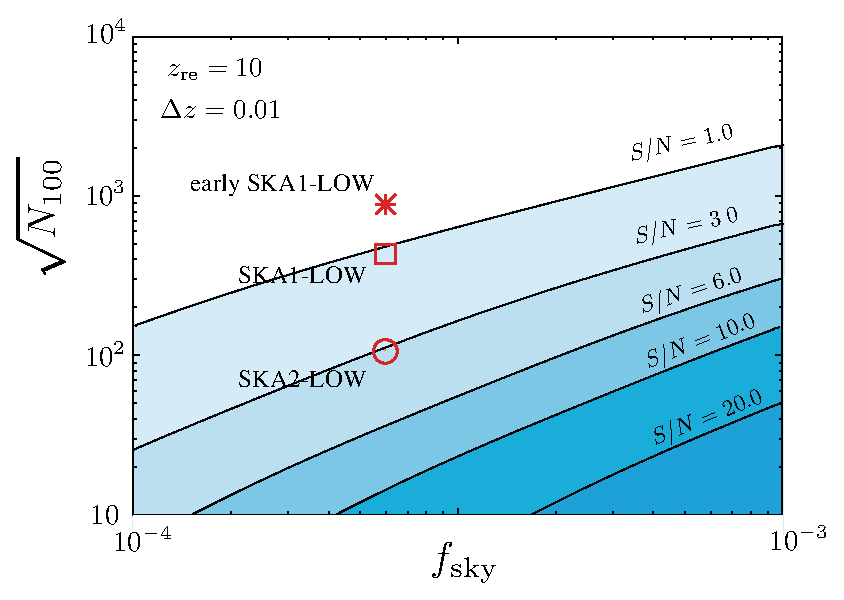
\includegraphics[width=70mm]{EoR/c03/c03.s2.f18.eps}
  \end{center}
 \end{minipage}
 \begin{minipage}{0.5\hsize}
  \begin{center}
   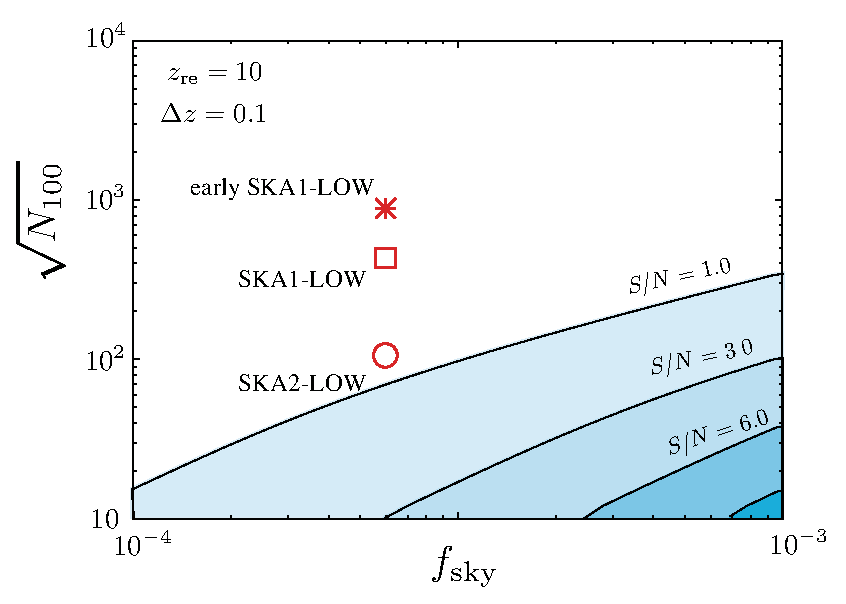
\includegraphics[width=70mm]{EoR/c03/c03.s2.f19.eps}
  \end{center}
 \end{minipage}
  \caption{$B:F%$%*%s2=%b%G%kKh$N(B21~cm$B$H(BCMB$B$NAj8_Aj4X$N(BS/N$BHf!#2#<4$O(B21~cm$B@~4QB,$N(B
 sky~fraction$B!"=D<4$OB?=E6K(B$\ell =100$$B$G5,3J2=$5$l$?4QB,$N%N%$%:%Q(B
 $B%o!<(B~($B%N%$%:$N3QEY%Q%o!<%9%Z%/%H%k(B$N(\ell)$$B$O(B$N(\ell )
 =N_{100}(\ell/100)^2$$B$GM?$($i$l$k(B)$B!#:8%Q%M%k$G$O(B$\Delta z = 0.01$$B!#(B
 $B1&%Q%M%k$G$O(B$\Delta z = 0.1$$B!#N>%Q%M%k$H$b(B$z_{\rm re} = 10$$B$G$"$j!"4QB,(B
 $B<~GH?t$O(B$z=10$$B$KBP1~$9$k!#(B}
  \label{fig:cmb_cross}
\end{figure}




\subsubsection{$B9b@VJ}JP0\6d2O$H$NAj8_Aj4X(B}

$B6d2O$OL)EY$f$i$.$N%H%l!<%5!<$G$"$k$HF1;~$K!"M-NO$J1'Ch:F%$%*%s2=8;$N0l$D(B
$B$H$7$F9M$($i$l$F$$$k!#$=$N$?$a!"1'ChO@E*(B21~cm$B@~$N%7%0%J%k$N6/$5$H6d2O$N(B
$B?tL)EY$H$NAj8_Aj4X$O!"1'Ch$N%$%*%s2=EY$K1~$8$F!"$9$3$7J#;($JMMAj$r<($9(B~\citep{2009ApJ...690..252L,2013MNRAS.432.2615W}$B!#(B

\begin{figure}[!t]
  \begin{center}
   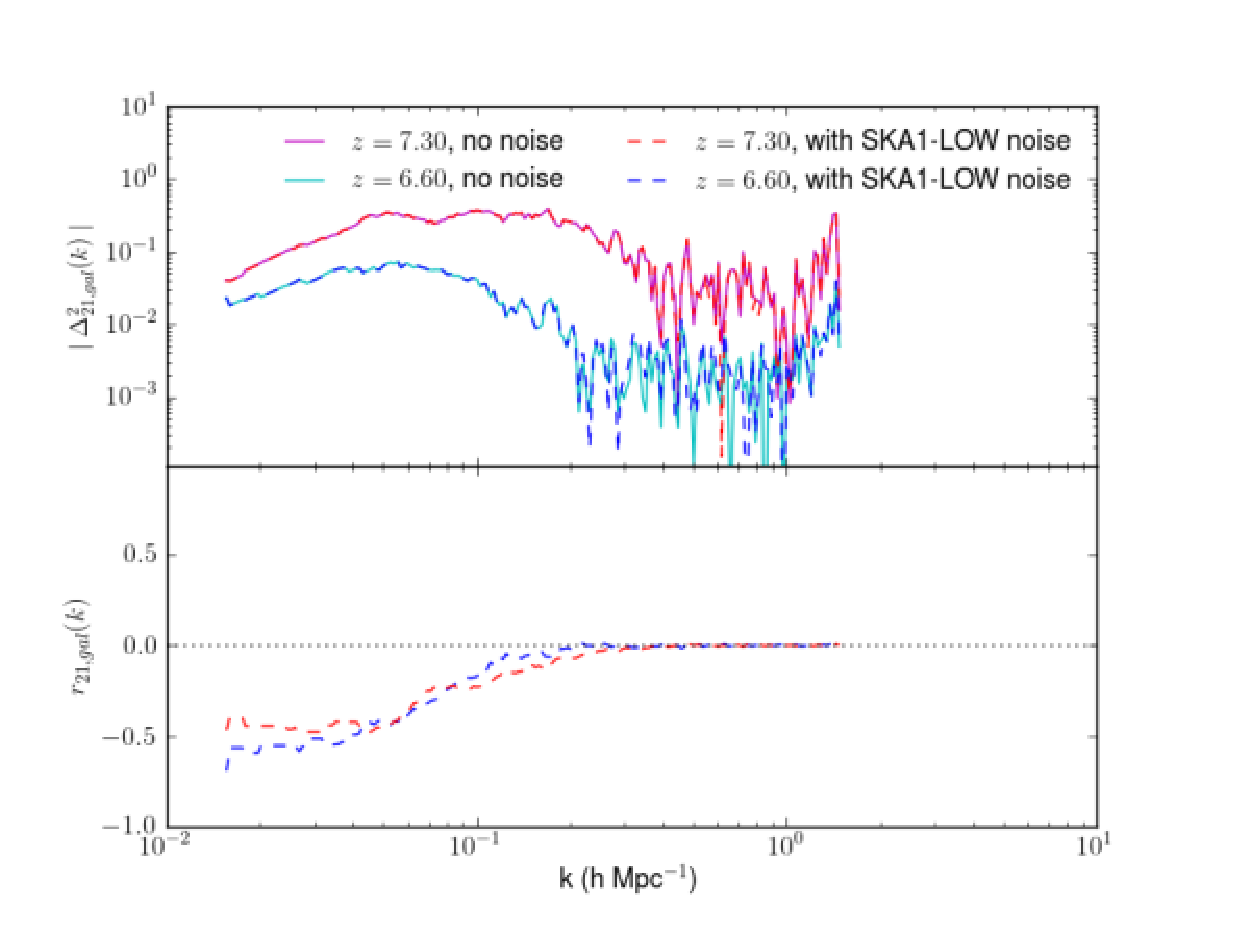
\includegraphics[width=100mm]{EoR/c03/c03.s2.f20.eps}
  \end{center}
 \caption{21~cm$B@~$H6d2O$NAj8_Aj4X$NL5<!852=$5$l$?%Q%o!<%9%Z%/%H%k!J>e%Q%M%k!K$H$=$NAj(B
 $B4X78?t!J2<%Q%M%k!K!#$3$3$GAj4X78?t(B$r$$B$O(B,$B6d2O$H(B21~cm$B@~$NL5<!85%Q%o!<%9%Z%/%H%k!"(B
 $\Delta^2(k)_{\rm halo}$$B$H(B$\Delta^2(k)_{21}$$B$rMQ$$$F!"(B
 $r=\Delta^2(k)_{21,\rm halo}/ \Delta^2(k)_{\rm halo} \Delta^2(k)_{21}$$B!#(B
 }
  \label{fig:galaxy_cross}
\end{figure}
\begin{figure}[!h]
 \begin{minipage}{0.5\hsize}
  \begin{center}
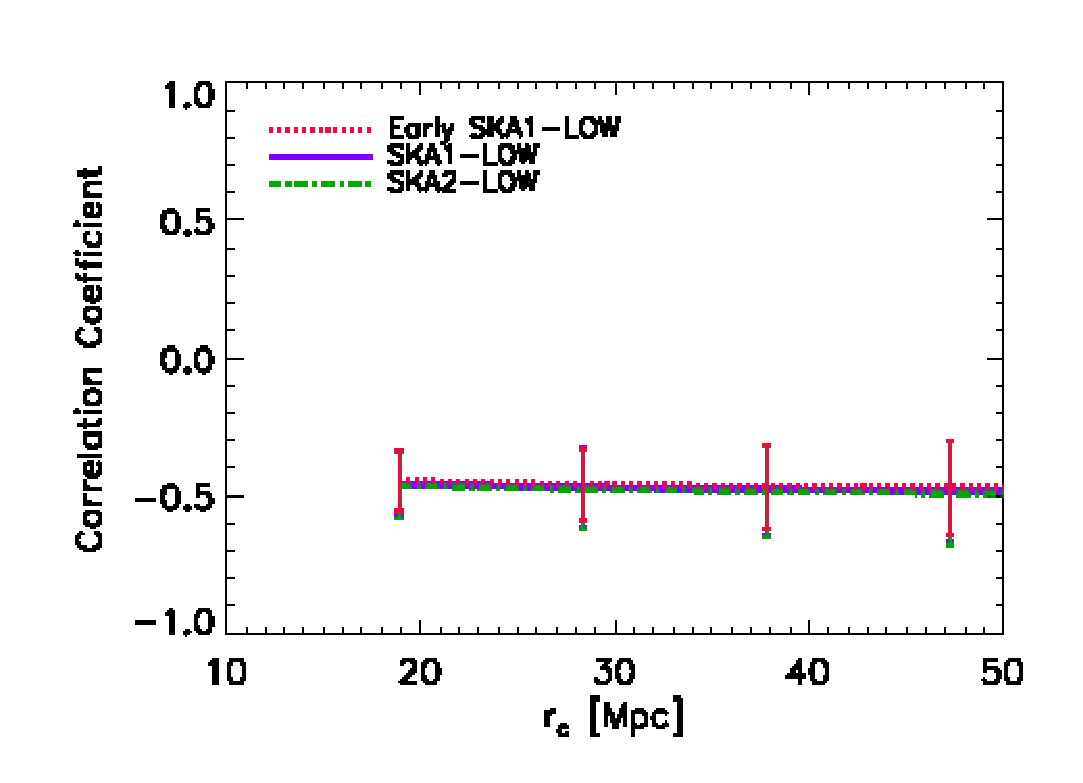
\includegraphics[width=70mm]{EoR/c03/c03.s2.f21.eps}
  \end{center}
 \end{minipage}
 \begin{minipage}{0.5\hsize}
  \begin{center}
   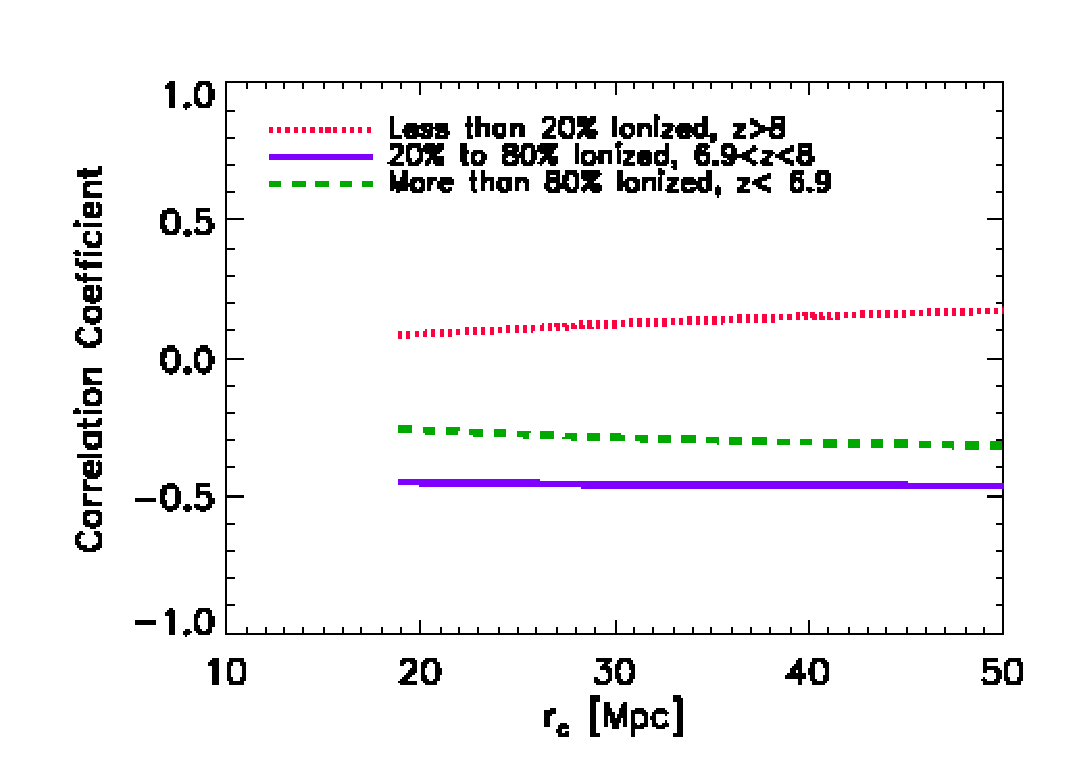
\includegraphics[width=70mm]{EoR/c03/c03.s2.f22.eps}
  \end{center}
 \end{minipage}
  \caption{$B6a@V30$H(B21~cm$BAj8_Aj4X78?t$X$N(BSKA$B$N46EY!J:8%Q%M%k!K$H%$%*%s2=(B
 $BN((B($B@VJ}JP0\(B)$B0MB8@-!J1&%Q%M%k!K!#(B}
  \label{fig:nirb_cross}
\end{figure}

$B1'Ch:F%$%*%s2=A0!"$b$7$/$O$=$N=i4|$K$O!"1'ChO@E*(B21~cm$B@~$N%7%0%J%k$NBg$-(B
$B$5$OL)EY$f$i$.$NBg$-$5$KHfNc$9$k!#6d2O$N?tL)EY$b$^$?L)EY$f$i$.$NBg$-$5$K(B
$BHfNc$9$k$?$a!"N><T$NAj8_Aj4X$O@5Aj4X$H$7$F8=$l$k!#(B
$B1'Ch$N:F%$%*%s2=$,?J$`$H!"1'ChO@E*(B21~cm$B@~$N%7%0%J%k$NBg$-$5$OCf@-?eAG$,(B
$B$I$l$[$I%$%*%s2=$5$l$:$K;D$5$l$F$$$k$+$K0MB8$9$k!#6d2O$O%$%*%s2=8w;R$N6!(B
$B5k8;$H$J$j$($k$N$G!"EvA3!"6d2O$N?tL)EY$,B?$$$H$3$m$G$O!"B?$/$N?eAG$,%$%*(B
$B%s2=$5$l$k$3$H$K$J$k!#$=$N$?$a!"%$%*%s2=$5$l$F$$$kNN0h!J%$%*%s2=%P%V%k!K$O!"(B21~cm$B@~$H6d2O(B
$B$NAj8_Aj4X$K$*$$$F$O!"Ii$NAj4X$H$7$F8=$l$k!#(B
$B$7$?$,$C$F!"Ii$NAj4X$N8=$l$k%9%1!<%k$N@VJ}JP0\$KBP$9$k?J2=$h$j!"%$%*%s2=%P%V(B
$B%k$N@.D9$r8+$k;v$,$G$-$k!#(B



$B?^(B~\ref{fig:galaxy_cross}$B$O:F%$%*%s2=$N%7%_%e%l!<%7%g%s$h$jF@$i$l$?(BEoR$B4|$NAj8_Aj(B
$B4X$N%Q%o!<%9%Z%/%H%k$r<($7$F$$$k(B~\citep{2013MNRAS.432.2615W}$B!#?^$N2<%Q%M(B
$B%k$r$_$k$H(B$z=9$$B$G(B$k \sim 0.3-0.4~h{\rm Mpc}^{-1}$$B$G8=$l$F$$$k(B
$BH?Aj4X$,:F%$%*%s2=$,?J$`$K$D$l$FBg$-$J%9%1!<%k$K0\F0$7$F$$$k!#(B
$B$7$?$,$C$F!"9b@VJ}JP0\6d2O$H(B21~cm$B@~$NAj8_Aj4X$r$H$l$P!"(B
$B$=$l$>$l$N@VJ}JP0\$G$NE57?E*$J%P%V%k%5%$%:$K%"%/%;%9$G$-$k2DG=@-$,$"$k;v(B
$B$,$o$+$k!#(B





\subsubsection{NIRB$B$H$NAj8_Aj4X(B}


$B1'Ch=i4|$N6d2O$d@1!9$O!"1'Ch:F%$%*%s2=$N$?$a$NM-8z$J%$%*%s2=8w;R6!5k8;$G(B
$B$"$k!#$7$?$,$C$F!"9b@VJ}JP0\$N@17A@.;K$rM}2r$9$k;v$O!"1'Ch:F%$%*%s2=;K$X$NM}2r$X$H$D$J$,$k!#(B
$B8=:_$N4QB,$K0M$l$P!"1'Ch$N:F%$%*%s2=$N$?$a$K$O8=:_4QB,$5$l$F$$$k6d2O$d@1!9(B
$B$h$j$b$5$i$KB?$/$N0E$/$F4QB,$5$l$F$$$J$$6d2O$d@1$,I,MW$G$"$k$3$H$,L@$i$+(B
$B$K$5$l$?!#$3$l$i$N@1$O2D;k8w$G$O4QB,$9$k$K$O0E$/$F$b!"@V(B
$BJ}JP0\$N7k2L!"6a@V30@~$GGX7JJ|<M$N0lIt$H$7$F51$$$F$$$k$3$H$,4|BT$5$l$F$$$k!#(B
$B$=$N$?$a!"6a@V30@~$NGX7JJ|<M$N4QB,$O!"1'Ch=i4|$N@1$N7A@.N($d$=$NJ,I[$NM}(B
$B2r$N=EMW$J%-!<$G$"$k(B~($B4XO"%l%S%e!<$H$7$F!"Nc$($P(B
\cite{2005PhR...409..361K}$B$r8+$h(B)$B!#(B


$B$9$G$K2?EY$b=R$Y$F$$$k$h$&$K!"(BEoR$B$+$i$N1'ChO@E*(B21~cm$B@~$N%7%0%J%k$N6/$5$O!"Cf@-?e(B
$BAG$NL)EY$K0MB8$7$F$$$k!#$9$J$o$A!"$=$N%7%0%J%k$N6/$$NN0h$O@1$d6d2O$,>/(B
$B$J$/!"?eAG$,%$%*%s2=$5$l$:$K<h$j;D$5$l$F$$$kNN0h$G$"$k!#(B
$BEvA3!"$=$NNN0h$O@1$d6d2O$,>/$J$$$N$G!"6a@V30@~$G8+$k$H0E$$!#(B
$B5U$K8@$($P!"6a@V30@~$G$_$FL@$k$$NN0h$O!"%$%*%s2=8w;R6!5k8;$G$"$k6d2O$d@1(B
$B$,B?$$NN0h$J$N$G!"1'ChO@E*(B21~cm$B@~$N%7%0%J%k$O<e$/$J$k!#(B
$B$D$^$j!"1'ChO@E*(B21~cm$B@~$H(BNIRB$B$N6/$5$OH?Aj4X$N4X78$K$"$k(B~\citep{2014MNRAS.440..298F}$B!#(B

\cite{2014MNRAS.440..298F}$B$O1'Ch=i4|$N6d2O(B
$B$K$h$k:F%$%*%s2=$N%7%_%e%l!<%7%g%s$r9T$$!"1'ChO@E*(B21~cm$B@~$H(BNIRB$B$NAj8_Aj(B
$B4X$r5a$a$?!#?^(B~\ref{fig:nirb_cross}$B$N:8%Q%M%k$,<($9$h$&$K!":F%$%*%s2=$N(B
$B?J9T$H$H$b$KH?Aj4X$N%7%0%J%k$OBg$-$/$J$j!"1'Ch$NBgH>$,:F%$%*%s2=$5$l$k$H(B
$B$=$N%7%0%J%k$O>.$5$/$J$C$F$$$/!#?^(B~\ref{fig:nirb_cross}$B$N1&%Q%M%k$O(B
$6 < z < 30$$B$+$i$N(BNIRB$B$H(B$6.4 < z < 11.1$$B$+$i$N(B21~cm$B@~$H$NAj8_Aj4X$rI=$7(B
$B$F$$$k!#$3$N?^$N%(%i!<%P!<$O(BLOFAR$B$N46EY$K4p$E$$$?$b$N$G$"$j!"(BSKA$B$G$O99$K(B
$B>.$5$$%(%i!<%P!<$,4|BT$5$l$F$$$k!#(B
%宇宙論的観測と中性水素21~cm線の相互相関
\subsection{$BJ?6Q%7%0%J%k(B}\label{c03.s3.ss1}
$B@VJ}JP0\$7$?(B21cm$B@~$rA4E7$KOJ$C$F4QB,$9$k$3$H$K$h$j!"J?6QE*$J1'Ch$NG.;K$r(B
$BCN$k$3$H$,$G$-$k$H4|BT$5$l$F$$$k!#FC$K:F%$%*%s2=$N%7%0%J%k(B
$B!J(BLyman-$\alpha$$B@~(B$\cdot$X$B@~$N8z$-;O$a$H8wNL!":FEEN%$N3+;O;~4|$H4|4V!"I8(B
$B=`%b%G%k$r1[$($?2CG.8;$NM-L5!K$O(BSKA-low (40GHz-200MHz)$B!"@2$l>e$,$j;~$N:F(B
$B7k9g@~$O(BSKA-mid$B$G$N%?!<%2%C%H$H$J$C$F$$$k!#(B

$BA4E7$N4QB,$K$D$$$F$O!"(BSKA$B$N$h$&$JBg5,LO$J43>D7W%7%9%F%`$O86M}E*$K$OI,MW$G(B
$B$O$J$/!"4{$K(Bsystematic dominated$B$J4QB,$K$J$C$F$*$j!"<B:]$K(BCoRE, EDGES,
LEDA, DARE, SARAS, SCI-HI, ZEBRA$B$J$I$N4QB,$,<B;\(B$\cdot$$B7W2h$5$l$F$$$k!#:G(B
$B?7$N4QB,$N0lNc$H$7$F(BSCI-HI$B$K$h$k7k2L$r<($9(B \citep{2014ApJ...782L...9V}$B!#(B
$B?^(B(\ref{fig:ichiki.fig.1})$B$NNP?'$K$h$k%G!<%?$,(B Global Sky Model
\citep{2008MNRAS.388..247D}$B$K$h$C$F(B 
$BA07JJ|<M$r?dDj$7:9$70z$$$?7k2L$N%Q%o!<$G$"$j!"@~$O:F%$%*%s2=%7%0%J%k$N(B
$B%b%G%k7W;;(B (3$B<oN`(B) $B$G$"$k!#$3$3$G$N<g$J7OE}8m:9$OA07JJ|<M$N:9$70z$-$N;D(B
$B:9$*$h$S%"%s%F%J%7%9%F%`$N<+8JL5@~<~GHK832(B (RFI)$B$G$"$k(B
$B$H5DO@$5$l$F$$$k(B \citep{2014ApJ...782L...9V}$B!#(B

\begin{figure}[!t]
\begin{minipage}[c]{0.49\linewidth}
\centering
{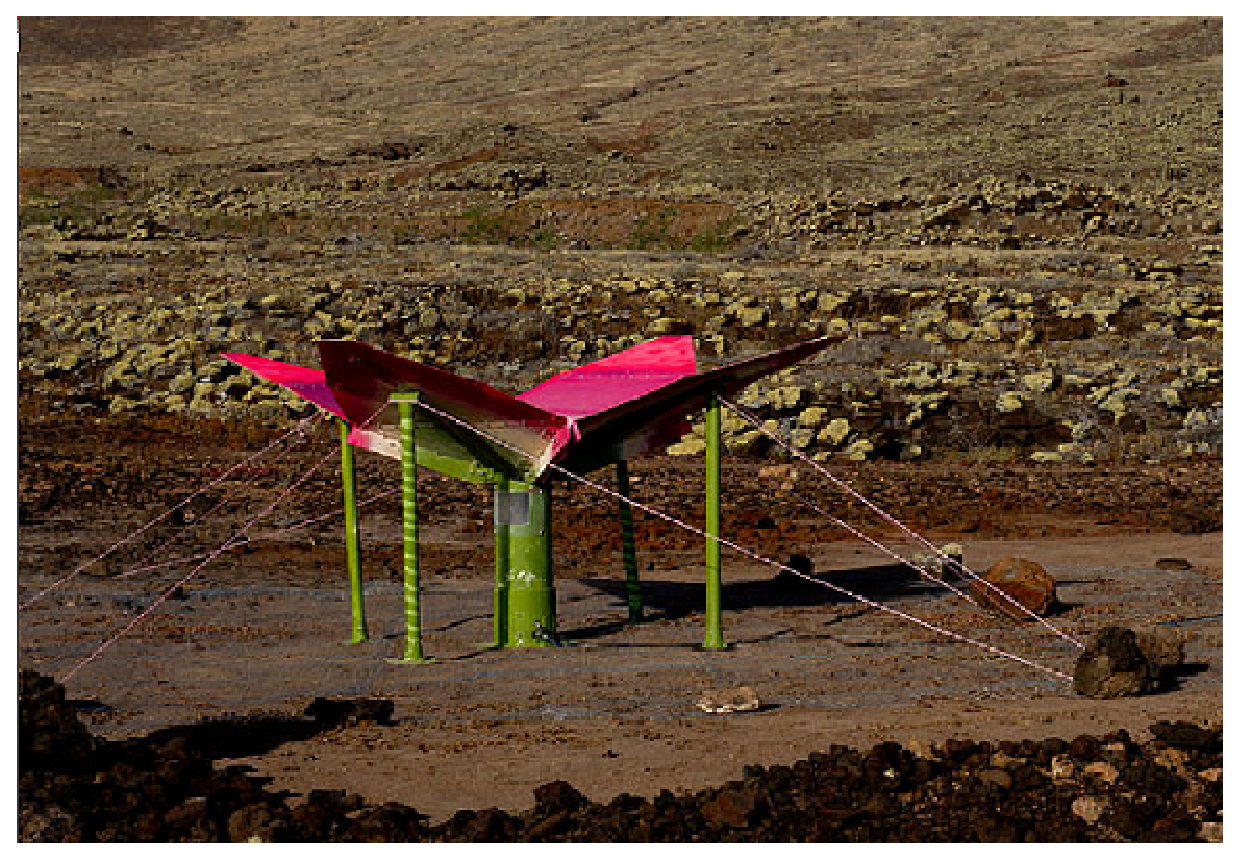
\includegraphics[width=\linewidth]{EoR/c03/c03.s2.f23.eps}}
\end{minipage}
\begin{minipage}[c]{0.49\linewidth}
\centering
{\includegraphics[width=\linewidth]{EoR/c03/c03.s2.f24.eps}}
\end{minipage}
\caption{Sonda Cosmologica de las Islas para la Deteccion de Hidrogeno
 Neutro (SCI-HI) $B$K$h$k4QB,Nc(B \citep{2014ApJ...782L...9V}$B!#(B}
\label{fig:ichiki.fig.1}
\end{figure}

$B$5$F!"$G$O$J$<43>D7W%7%9%F%`$G$"$k(BSKA$B$NK>1s6@$GE7$NJ?6QE*$J%7%0%J%k$,4QB,(B
$BBP>]$H$J$k$N$@$m$&$+!)$3$l$K$D$$$F$O43>D7W%7%9%F%`$r43>D7W$H$7$FMQ$$$:4Q(B
$BB,$9$kMxE@$H$7$F0J2<$N$h$&$J5DO@$,$"$k!#(B
\begin{itemize}
 \item $BA4E7%7%0%J%k4QB,$N:GBg$N7OE}8m:9$O%b!<%I%+%C%W%j%s%0!J<~GH?tKh$N(B
       $B%S!<%`$N0c$$$K$h$C$F6u4VJ}8~$NMI$i$.$,<~GH?tJ}8~$NMI$i$.$H:.$6$k!K(B
       $B$G$"$j!"$3$l$r<h(B
       $B$j=|$/<jK!$H$7$F(BSKA$B$N43>D7W%b!<%I$,M-8z!#(B
 \item $B43>D7W%7%9%F%`$K$h$k>\:Y4QB,$r9T$&%?!<%2%C%H@VJ}JP0\$r$^$:J?6Q%7(B
       $B%0%J%k$+$iC5$k!#(B
 \item $B29EY$N%<%mE@$rB,$k!J43>D7W%b!<%I$GF@$i$l$?%Q%o!<%9%Z%/%H%k$O5[<}(B
       $B$K$h$k$b$N$J$N$+!"J|<M$J$N$+!K!#(B
\end{itemize}
SKA$B$r$I$N$h$&$KMQ$$$k$+$K$D$$$F$OBg$-$/J,$1$FFsDL$j$,9M$($i$l$F$$$k!#$9(B
$B$J$o$A!"D>7B(B $35$ m$B$N(Bstation$B$r0l$D$NK>1s6@$H$7$FMQ$$$kJ}K!$G!";kLn$,(B
$5\times 5$ $BJ?J}EY$HHf3SE*69$/$J$k$?$aA07JJ|<M$N:9$70z$-$O$7$d$9$/$J$k$,!"(B
$B%b!<%I%+%C%W%j%s%0$,J#;($K$J$k!#$^$?$O(Bstation$B$K$"$k0l$D$N%"%s%F%J$@$1$r(B
$BK>1s6@$H$7$FMQ(B
$B$$$kJ}K!$G!"$3$N>l9g$O%b!<%I%+%C%W%j%s%0$O8:$k$b$N$N!";kLn$,(B$90\times 90$$BJ?J}EY(B
$B$H9-$/$J$jA07JJ|<M$N:9$70z$-$OFq$7$/$J$k!#(B

$B$^$?!"43>D7W$O0lHL$KA4E7$NJ?6Q(Bsignal$B$K$O46EY$,$J$$$,!"?)$r5/$3$7$F$$$kE7BN(B
$B!JNc$($P7n!K$,$"$l$P!"$N$C$Z$j$7$?A4E7%7%0%J%k$K6u4VE*$J9=B$$,@8$8$k$3$H(B
$B$K$J$j4QB,$,2DG=$H$J$k!#FC$K!"7n$O$[$\0lMM$J(B$230$K$B$N9uBNmU<M$@$H4|BT$5$l$F(B
$B$$$k$N$G!"$3$l$r4p=`$KA4E7%7%0%J%k$rB,$k$3$H$,$G$-$k!#<B:](BLOFAR$B$K$h$k<B(B
$B83$K$h$j!"LdBj$K$J$k$H;W$o$l$F$$$?CO5e$N(BRFI$BH?<MGH$OD94p@~(B ($\gtrsim
100\lambda$) $B4QB,$K$h$j%b%G%k2=$7:9$70z$1$=$&(B
$B$G$"$k$3$H!"(BSKA$BDxEY$N(Bfilling factor$B$,$"$l$P?tF|$N4QB,;~4V$G8!=P2DG=$G$"(B
$B$k$3$H$,L@$i$+$K$5$l$F$$$k!#(B

%平均シグナル


%\setcounter{section}{3}
\section{日本が狙うサイエンス}\label{c03.s3}
$B1'Ch$N:FEEN%$,$I$N$h$&$K$7$F5/$3$C$?$+!"$H$$$&LdBj$OM}O@E*$K$b4QB,E*$K$b(B
$BL$$@L@$i$+$K$5$l$F$$$J$$8&5f%F!<%^$G$"$k!#4QB,E*$K$O!":#8e(BSquare
Kilometre Array (SKA)$B$KBeI=$5$l$kBg7?$NDc<~GHEEGH43>D7W$K$h$j!"1sJ}1'Ch$G(B
$B$NCf@-?eAG(B21 cm$B@~4QB,$,Bg$-$/?JE8$9$k$3$H$,4|BT$5$l$F$$$k!#$=$3$G(BSKA-JP $B:F(B
$BEEN%HI$G$O!"F@$i$l$kKDBg$J4QB,%G!<%?$+$i1'Ch:FEEN%4|$K5/$-$?8=>]$rM}2r$9(B
$B$k$?$a$K!"4QB,%G!<%?$H$NHf3S$KBQ$($kM}O@%b%G%k$N9=C[$*$h$S4QB,E*M=8@$r9T(B
$B$&!#$^$?!"1sJ}1'Ch$N>pJs$rF@$k$?$a$K$OA07JJ|<M!"$H$/$K7O30$N%3%s%Q%/%H$J(B
$BEEGH8;$d7OFb$N%7%s%/%m%H%m%sJ|<M$,LdBj$K$J$k$H;XE&$5$l$F$$$k$3$H$+$i!"4{(B
$BB8$N4QB,AuCV$rMQ$$$F!"$3$l$i$N=|5n!&2sHr$K$D$$$F<B>ZE*$K8&5f$9$k!#(B

$B$9$J$o$A!"1'Ch:FEEN%4|$N>pJs$r==J,$K3hMQ$G$-$k$h$&$K$9$k$?$a!"(BSKA-JP $B:F(B
$BEEN%HI$G$O0J2<$NFs$D$r3hF0$NCl$H$9$k!#(B

\begin{itemize}
 \item[(1)] $BB.$/@53N$JM}O@%b%G%k7W;;$r9T$&7W;;%3!<%I$N3+H/(B
 \item[(2)] $BDc<~GHNN0h$NA07JJ|<M$N%b%G%k2=$H=|5nJ}K!$N9=C[(B
\end{itemize}

$B0J2<$G$O!"$^$:4{B8$N7W;;%3!<%I(B21cmFAST$B$N>\:Y$r5-$7!"(B
$B$=$NLdBjE@$r;XE&$7$?$N$A!"(BSKA-JP$B$N@oN,$r5-=R$9$k!#(B

\subsection{$B4{B8$N7W;;<jK!!J(B21cmFAST$B$rNc$K$7$F!K(B\label{sec.21cmFAST}}
$B8=:_MxMQ2DG=$J1'Ch:FEEN%4|$N=`2r@OE*$J7W;;%3!<%I$O(BSimFast21(\citep{2010ascl.soft10025S})$B$d(B21cmFAST(\citep{2011MNRAS.411..955M})$B$,$"$k!#$3$l$i$N7W;;%3!<%I$O(B
$B%$%*%s2=$dL)EY?J2=Ey$rMM!9$J6a;w$rMQ$$$F7W;;$7!"J#;($J1'Ch:FEEN%4|$NMM;R(B
$B$r:F8=$7$h$&$H$9$k$b$N$G$"$k!#(B

21cmFAST$B$O(B21cm$B@~51EY29EY$N;0<!85%^%C%W$r7W;;$9$k;v$,$G$-$k!#(B21cmFAST$B$N%3!<(B
$B%IFb$G(B21cm$B@~$N51EY29EY$O(B(3.1)$B<0$G7W;;$5$l$k!#(B 
\begin{eqnarray}
{\delta}T_{b}(\nu)&=&\frac{T_{s}-T_{\gamma}}{1+z}(1-e^{-\tau_{\nu_{0}}})\nonumber\\
  &\approx&27x_{{\rm HI}}(1+\delta_{m})\left(\frac{H}{dv_{r}/dr+H}\right)\left(1-\frac{T_{\gamma}}{T_{s}}\right)\left(\frac{1+z}{10}\frac{0.15}{\Omega_{m}h^{2}}\right)^{\frac{1}{2}}\left(\frac{\Omega_{b}h^{2}}{0.023}\right)[\rm mK]
\end{eqnarray}
$B%P%j%*%s$NL)EYMI$i$.(B$\delta_m$$B!"Cf@-N((B$x_{{\rm HI}}$$B!"%9%T%s29EY(B$T_s$$B!"(B
$BB.EY8{G[(B$dv_r/dr$$B$G$"$k!#$^$:!"$3$l$i#4$D$NNL$,#3<!85$N%^%C%W$H$7$F7W;;(B
$B$5$l!"$=$l$i$rMQ$$$F51EY29EY$N%^%C%W$r7W;;$9$k!#(B 
$B0J2<$G$O$^$:!"(B21cmFAST$B$G$3$l$i$NNL$r$I$N$h$&$K7W;;$7$F$$$k$+$^$H$a$k!#(B 

$B$^$:!"L)EY>l$K$D$$$F!#L)EY>l$N7W;;$O%<%k%I%S%C%A6a;w$rMQ$$$F9T$o$l$k!#(B
$BL)EY$N>pJs$O;0<!85$N%^%C%W$N%;%k$4$H$KM?$($i$l$k!#$3$NL)EY>l$N>pJs$r$b$H(B
$B$K;D$j$N#3$D$NNL$O7W;;$5$l$k!#(B 
$BF@$i$l$?L)EY>l$N%^%C%W$+$i!"%$%*%s2=N((B$x_{{\rm HII}}$$B$N7W;;$r9T$&!#Cf@-N($O(B$x_{{\rm HI}}=1-x_{{\rm HII}}$$B$G$"$k!#(B
21cmFAST$B$GMQ$$$i$l$F$$$k%$%*%s2=$NH=Dj$N<0$O3FE@(B$x$$B$H3F@VJ}JP0\(B$z$$B$K$*$$$F<!$N$h$&$K=q$1$k!#(B
\begin{eqnarray} 
f_{coll}(x,z,R)\geq\zeta^{-1}
\end{eqnarray}
$\zeta$$B$O%$%*%s2=8zN($H8@$C$F!"6d2O$,<~0O$NJ*<A$r%$%*%s2=$9$k8zN($rI=$9!#(B
$B%$%*%s2=$NH=Dj$G$O$^$:!"$"$k%;%k$N<~0O$KH>7B(B$R$$B$N5e$r9M$($k!#$3$N(B$R$$B$O%$%*%s2=8w;R$NJ?6Q<+M39TDx$KBP1~$7!"(B21cmFAST$B$G$O%Q%i%a!<%?$H$7$FDj?t$GM?$($i$l$k!#$3$N5eCf$NJx2uHf(B $f_{coll}$$B$r7W;;$7$F>e<0$KEv$F$O$a$k!#(B$f_{coll}$$B$O5eA4BN$N<ANLL)EY$H!"5eCf$G==J,$KJx2u$7$?<ANLL)EY$NAmOB$H$NHf$G$"$k!#>r7o$rK~$?$7$F$$$k$J$i!"$=$N%;%k$K$O%$%*%s2=$9$k$N$K==J,$JNL$N8w;R$,B8:_$9$k$H$7$F%$%*%s2=$7$?$H$_$J$7!"Cf@-N($r(B0$B$H$9$k!#>r7o$rK~$?$7$F$$$J$$>l9g!"5e$NH>7B$r=L$a$FF1MM$NA`:n$r9T$&!#>r7o$rK~$?$9$^$G7+$jJV$7!":G>.$N(B$R$(1grid$B$NBg$-$5(B)$B$^$G>r7o$,K~$?$5$l$J$+$C$?>l9g!"$=$N%;%k$N%$%*%s2=N($O(B$\zeta f_{coll}$$B$H$9$k!#$3$NA`:n$rA4%;%k$KBP$7$F9T$&!#(B

$B%9%T%s29EY$O:FEEN%0JA0$N51EY29EY$GFC$K=EMW$K$J$k!#$^$?!"(B21cmFAST$B$N7W;;$NCf$G:G$bJ#;($G;~4V$N$+$+$kItJ,$G$"$k!#%9%T%s29EY$N7W;;$O(B(3.2)$B<0$G9T$o$l$k!#(B
\begin{equation}
T_S^{-1}=\frac{T_{\gamma}^{-1}+x_{\alpha}T_{\alpha}^{-1}+x_cT_K^{-1}}{1+x_c+x_{\alpha}}\nonumber
\end{equation}
$T_{\gamma}$$B$O(BCMB$B29EY!"(B$T_K$$B$O%,%929EY$G$"$k!#(B$T_{\alpha}$$B$O(BLyman-$\alpha$$B?'29EY$G$"$k$,!"(B$T_{\alpha}=T_K$$B$H$$$&6a;w$rMQ$$$k$N$G<B:]$K$O%,%929EY$r7W;;$9$k!#(B
$x_c$$B$O>WFM78?t$G$"$k!#7W;;<0$O(B
\begin{equation}
x_c=\frac{0.0628 K}{A_{10}T_{\gamma}}[n_{{\rm HI}}\kappa^{HH}_{1-0}(T_K)+n_{e}\kappa^{eH}_{1-0}(T_K)+n_{p}\kappa^{pH}_{1-0}(T_K)]
\end{equation}
$B$H$J$k!#(B$A_{10}$$B$O<+A3J|<M78?t$G$"$k!#E:;z$O(B(${\rm HI},e,p$)=($BCf@-?eAG(B,$BEE;R(B,$BM[;R(B)$B$rI=$7$F$$$k!#(B$n_i$$B$O$=$l$>$l$N?tL)EY$G$"$k!#(B$\kappa$$B$O%,%929EY$K0MB8$9$k>WFM8zN($G$"$j!"BP1~$9$k?tCM$,MQ0U$5$l$F$$$k!#(B
$B%,%929EY$N7W;;$O<!$N<0$rMQ$$$k!#(B
\begin{equation}
\frac{dT_K({\bf{x}},z')}{dz'}=\frac{2}{3k_B(1+x_e)}\frac{dt}{dz'}\sum_p\epsilon_p+\frac{2T_K}{1+z'}
+\frac{2T_K}{3}\frac{dD(z')/dz'}{D(z)/\delta_{nl}({\bf{x}},z)+D{z'}}
-\frac{T_K}{1+x_e}\frac{dx_e}{dz'}
\label{TK}
\end{equation}
$B$H$J$k!#<0(B(\ref{TK})$B$NBh0l9`$OMM!9$J%W%m%;%9$N2CG.$N8z2L$G(B$\epsilon_p$$B$O$"$k2aDx(B($p$)$B$G$N2CG.N($rI=$9!#BhFs9`$O%O%C%V%kKDD%$N8z2L!"Bh;09`$O9=B$7A@.$KH<$&CGG.E*$J2CG.$HNd5Q$N8z2L!"Bh;M9`$O%$%*%s2=$K$h$k%,%9N3;R?t$NJQ2=$rI=$9!#(B
$B2CG.$N%W%m%;%9$O%3%s%W%H%s;6Mp$H(BX$B@~J|<M$r9MN8$9$k!#(B
X$B@~J|<M$K$h$k2CG.$N7W;;$O%^%C%W$N3F%;%k$4$H$K9T$o$l$k!#6qBNE*$K$O!"%;%k$rCf?4$K5e3L$r9M$($k!#$=$N5e3LCf$G(B$f_{coll}$$B$r7W;;$7!"9M$($F$$$k%;%k$KE~C#$9$k(BX$B@~$NJ|<M8w;R$NNL$r8+@Q$b$k!#$3$N:]!"==J,1sJ}$+$i$N(BX$B@~J|<M$N4sM?$r8+@Q$b$k$?$a!"@VJ}JP0\(B$z$$B$K4X$9$k@QJ,$G7W;;$5$l$k!#(B

$x_{\alpha}$$B$O(BLyman-${\alpha}$$B9`8w;R$H$N>WFM78?t$G$"$j!"<!$N$h$&$K=q$1$k!#(B
\begin{equation}
x_{\alpha}=1.7\times10^{11}(1+z)^{-1}S_{\alpha}J_{\alpha}
\end{equation}
$B$3$3$G(B$S_{\alpha}$$B$O86;RJ*M}$r9MN8$7$?=$@578?t!"(B$J_{\alpha}$$B$O(BLyman-$\alpha$$B$NGX7JJ|<M$G$"$k!#(B
Lyman-$\alpha$$B$NGX7JJ|<M$O#2$D$N4sM?$r7W;;$9$k!#0l$D$O(BX$B@~$K$h$C$FNe5/$5$;$i$l$?(BHI$B$+$i$NJ|<M$G!"(BX$B@~$K$h$k2CG.$HF1MM$K5e3L$+$i%;%k$X$N4sM?$r7W;;$9$k!#$b$&0l$D$O@1$+$iJ|<M$5$l$?(BLyman-n$B8w;R$,(BLyman-$\alpha$$B$K%+%9%1!<%I$9$k8z2L$G$"$k!#$3$A$i$b5e3L$+$i$N4sM?$r9M$($k!#(B
$B$^$?!"B.EY8{G[$K$D$$$F$O3F%;%k$NL)EY>l$H@~7A@.D90x;R(B$D(z)$$B$N;~4VHyJ,$rMQ$$$F<!$N<0$G7W;;$5$l$k!#$?$@$7!"$3$N9`$K4X$7$F$O%U!<%j%(6u4V(B${\bf{k}}$$B$G7W;;$7$F$$$k!#(B
\begin{eqnarray}
\frac{dv_{r}}{dr}({\bf k},z)\approx-\frac{{k_{r}}^2}{k^2}\dot{D}(z)\delta_{nl}({\bf k})
\end{eqnarray}

$B:G8e$K!"F@$i$l$?;M$D$N%^%C%W$+$i%;%k$4$H$K51EY29EY$r7W;;$9$k!#$5$i$K!"F@$i$l$?51EY29EY$N%^%C%W$rMQ$$$F%Q%o!<%9%Z%/%H%k$r7W;;$9$k!#<B:]$K(B21cmFAST$B$K$h$C$F7W;;$5$l$?%Q%o!<%9%Z%/%H%k$H%7%_%e%l!<%7%g%s$N7k2L$rHf3S$7$?$N$,?^(B\ref{fig:ps}$B$G$"$k!#(B
\begin{figure}
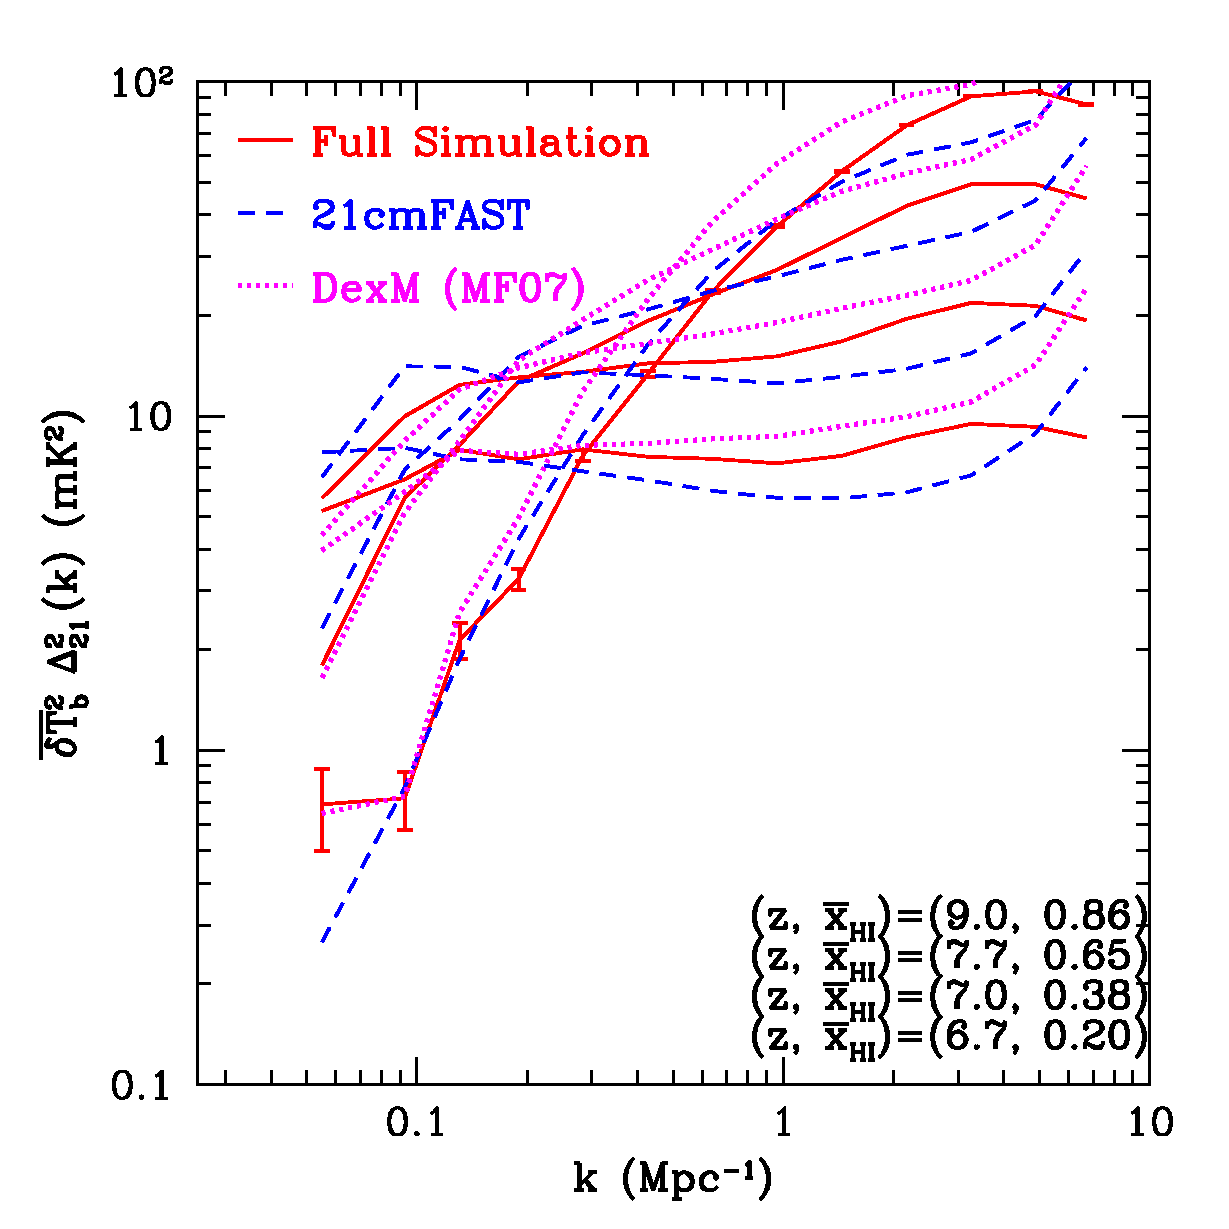
\includegraphics[width=0.6\linewidth]{EoR/c03/c03.s3.f1.eps}
\centering
\caption{$B%7%_%e%l!<%7%g%s7k2L!J@V@~!K!"(B21cmFAST$B$N7k2L!J@D?'!K!"(BDeXM(21cmFAST$B$NA0?H(B)$B$N7k2L!J%^%<%s%?!K(B}
\label{fig:ps}
\end{figure}
$B0J>e$,(B21cmFAST$B$G9T$o$l$k7W;;$N35N,$G$"$k!#(B
%既存の計算手法(21cmFASTを例にして)
\subsection{$BLdBjE@(B}\label{c03.s3.ss2}
$B>e$G=R$Y$?$h$&$K!"(B21cmFAST$B$G$O7W;;%3%9%H$r8:$i$9$?$a$K!"L)EY>l$N7W;;$d%9(B
$B%T%s29EY$N7W;;$K6a;w$,MQ$$$i$l$F$$$k!#(B  21cmFAST$B$N7W;;$K$*$1$kLdBjE@$O<g(B
$B$K$=$N6a;w$,860x$G$"$k!#0J2<$G$O(B21cmFAST$B$N6a;w$NLdBjE@$d!"9MN8$5$l$F$$$J(B
$B$$=EMW$JJ*M}$K4X$7$F(B10$B9`L\$K$^$H$a$k!#(B
\begin{itemize}
\item 21cmFAST$B$G$O!"%$%*%s2=N($dB.EY8{G[$N7W;;$OL)EY>l$r$b$H$K9T$o$l$k!#$7$+$77W;;$KMQ$$$i$l$F$$$k%<%k%I%S%C%A6a;w$OBg%9%1!<%k$N6a;w$H$7$F$h$/MQ$$$i$l$k$,!">.%9%1!<%k(B($k>1$)$B$N7W;;$G$O%7%_%e%l!<%7%g%s7k2L$H$N%:%l$,Bg$-$/$J$k!#"*(BN$BBN7W;;$N7k2L$rAH$_9~$a$P$$$$!)(B
\item $BL)EY>l$O=ENO$N8z2L$N$_$G7W;;$5$l$F$*$j!"%@!<%/%^%?!<$NL)EYJ,I[$r7W;;$7$F$$$k;v$K$J$C$F$$$k!#K\Mh$J$i%@!<%/%^%?!<$H%P%j%*%s$NL)EYJ,I[$N4V$N4X78$r9MN8$7$J$/$F$O$J$i$J$$!#"*AjBPB.EY$N8z2L$b<h$jF~$l$i$l$k!)(B
\item $BL)EY>l$+$i8D!9$NJ|<M8;$rF1Dj$;$:!"%W%l%9%7%'%R%?!<M}O@$rMQ$$$FJ*<A$NL)EY$+$i5eCf$GAmOB$N8w;R$NJ|<MNL$r7W;;$7$F$$$k!#(B
\item $B;H$($k%Q%i%a!<%?$N?t$,>/$J$/!"$^$?!"K\Mh$J$i@VJ}JP0\$d6u4V0MB8@-$r;}$D%Q%i%a!<%?$,Dj?t$H$7$F07$o$l$F$$$k!#(B
\item $B%$%*%s2=H=Dj$N(B$\zeta$$B$OK\Mh<!$N$h$&$KI=$5$l$k!#(B
\begin{eqnarray} 
\zeta=\frac{Nf_{*}f_{esc}}{1+\bar{n}_{rec}}
\end{eqnarray}
      $B$3$3$G!"(B$N$$B$O%P%j%*%sEv$?$j$N%$%*%s2=8w;R$N?t!"(B$f_{\rm esc}$$B$O%$%*%s2=8w(B
      $B;R$,6d2O$+$i(BIGM$B$KH4$1=P$93d9g!"(B$f_*$$B$O6d2O$N%,%9$NCf$G!"@1$K$J$C$F(B
      $B$$$k%P%j%*%s$N3d9g$G$"$k!#(B21cmFAST$B$G$O$3$N(B$\zeta$$B$O0lDjCM$H$J$C$F(B
      $B$$$k$,!"<0$r8+$k$HJ,$+$k$h$&$KC&=P8w;RN($d:F7k9gN((B $n_*$$B$J$I$K4X78(B
      $B$7$F$$$k$N$G>l=j$K$h$C$F$=$NCM$OJQ2=$9$k$O$:$G$"$k!#(B 
\item $B%$%*%s2=$rH=Dj$9$k:]!"$O$8$a$KH>7B(B$R$$B$N5e$r9M$($k$,!"$3$N(B$R$$B$O(B
      21cmFAST$B$G$O0lDjCM$H$J$C$F$$$k!#(B$R$$B$O%$%*%s2=8w;R$NJ?6Q<+M39TDx$J(B
      $B$N$GK\Mh$J$iCf@-?eAG$NL)EY$J$I$K0MB8$5$;$kI,MW$,$"$k!#(B 
\item $B%/%i%s%T%s%0%U%!%/%?!<$b%Q%i%a!<%?$H$7$F0lDj$K$J$C$F$$$k$,!"$3$NCM(B
      $B$O(B$z$$B$K$h$C$FJQ2=$9$k>e$K!"L)EY$NG;$$=j$H$=$&$G$J$$$H$3$m$GCM$,0[(B
      $B$J$k;v$,CN$i$l$F$$$k!#L)EY$NG;$$$H$3$m$G$O:F7k9g$K$h$C$F%$%*%s2=$5(B
      $B$l$F$$$?(B${\rm H}_{\textsc{II}}$$B$,(B${\rm H}_{\textsc I}$$B$KLa$k!#$=$N$?$a!"$=$N>l=j$r40A4$K%$%*%s2=$9$k$K$O(B
      $BCf@-?eAG$N?t0J>e$N%$%*%s2=8w;R$,I,MW$K$J$k!"$H$$$&8z2L$r<h$jF~$l$k(B
      $BI,MW$,$"$k!#(B 
\item $B@1$+$i$NJ|<M(B($B%U%#!<%I%P%C%/(B)$B$K$h$C$F9=B$7A@.$,M^@)$5$l$k8z2L$,9MN8(B
      $B$5$l$F$$$J$$!#(B 
\item 21cmFAST$B$G$O%$%*%s2=$O4pK\E*$K(BUV$B$G9T$o$l$k!#(BX$B@~$N$h$&$KJ?6Q<+M39T(B
      $BDx$NBg$-$$8w;R$K$h$k%$%*%s2=$O(BUV$B$G%$%*%s2=$7$-$l$F$$$J$+$C$?$H$3$m(B
      $B$K$N$_:nMQ$9$k$H$5$l$F$$$k!#(B 
\item $B$3$l$@$16a;w$7$F$b7W;;;~4V$,(B10$B;~4V$rD6$($k!#(B($B$?$@$7(B$z=5.6-35$, 80
      $B@VJ}JP0\(B, $200/300$ [Mpc/grids]$B$G$N7W;;$r(B8$B%9%l%C%I$K$h$kJBNs7W;;$r9T$C$?(B
      $B>l9g!#(B)$B7W;;;~4V$NHfN($O$@$$$?$$!"%9%T%s29EY$N7W;;$K(B7$B3d!"$=$NB>$N7W(B
      $B;;$G(B3$B3dDxEY$G$"$k!#(B 
\end{itemize}
%問題点
\subsection{SKA-JP $B:FEEN%HI$N@oN,(B}
%\label{EoR.s4}
\label{c03.s3.ss3}
\subsubsection{(1)$BF|K\HG(B21 cmFAST$B%3!<%I$N9=C[(B}
$B4QB,%G!<%?$+$i=iBeE7BN!&6d2O$N7A@.$K4X$9$k>pJs$rF@$k$?$a$K$O!"Hf3S$KBQ$((B
$B$k@:EY$r$b$DM}O@%b%G%k$N9=C[$,IT2D7g$G$"$k!#FC$KCf@-?eAG$+$i$N%7%0%J%k$r(B
$B?dDj$9$k$K$O!"0E9uJ*<A$H%,%9$N=ENOIT0BDj@-$K$h$k@.D9$K2C$(!"=iBeE7BN!&6d(B
$B2O$N7A@.$H$=$3$+$iJ|$?$l$k(BX$B@~!&;g30@~$K$h$k%,%9$N2CG.!&:FEEN%$r7W;;$7$J$1(B
$B$l$P$J$i$J$$!#(B

SKA$B$K$h$C$F:FEEN%4|$K$*$1$kCf@-?eAG(B21 cm$B@~$,4QB,$G$-$l$P!":FEEN%$N;~4|!"(B
$BH/E8$N;EJ}!"EEN%8w;R8;$J$I$3$l$^$GL$2rL@$G$"$C$?>pJs$rF@$k;v$,$G$-$k!#$^(B
$B$?!":FEEN%4|$O!"B>GHD9$N<!@$Be4QB,5!4o$N%?!<%2%C%H$H$J$C$F$$$k;~4|$G$"$j!"(B
$BB>GHD9$N4QB,7k2L$+$i$/$k@)8B$rMQ$$$l$P!":FEEN%$K4X$9$kM}2r$OHtLvE*$K?J$`(B
$B$H4|BT$G$-$k!#$7$+$7!"(B\ref{c03.s3.ss1}$B$d9q:]%5%$%(%s%9%V%C%/$N>R2p$NItJ,(B
$B$G$b$"$k$h$&$K!"$3$l$^$G$N8&5f$O!"J|<M8;E7BN$d6d2O4VJ*<A$N%b%G%j%s%0$K4X(B
$B$7$FITDj@-$,Bg$-$/!"8=>u$N$^$^$G$O>\:Y$JM}O@M=B,$O:$Fq$G$"$k!#(B

$B$3$N@a$G$O!"9q:]%5%$%(%s%9%V%C%/>R2p$N>O$G$9$G$K?($l$?@$3&$G9T$o$l$F$$$k(B
$B:FEEN%$N7W;;<jK!(B(\ref{c03.s2.ss2})$B$r$b$&0lEY4JC1$K>R2p$7!"$=$N8e(B SKA-JP$BFH(B
$B<+$N%"%W%m!<%A$*$h$S$=$l$K$h$C$F2~A1$5$l$kE@$r5-$9!#(B

\medskip 

$B$3$l$^$G!"1'Ch:FEEN%$NM}O@E*8&5f$O<g$K=`2r@O!&=`?tCME*7W;;!"$*$h$S?tCM%7(B
$B%_%e%l!<%7%g%s$K$h$C$F9T$o$l$F$-$?!#(B1-zone$B$N=`2r@OE*<jK!$G$O!"(B
Press-Schechter formalism$BEy$rMQ$$$F3F@VJ}JP0\$4$H$N(BDM$B%O%m!<<ANL4X?t$rF3=P(B
$B$7!"$=$3$KMM!9$J(BBaryonic Physics$B$r2>Dj$9$k;v$G!"1'Ch$NJ?6QE*$JG.!&EEN%?J(B
$B2=;K$r7W;;$9$k!#$3$N<jK!$O!">/$J$$7W;;NL$G1'Ch$NBg6IE*$J?J2=$rD4$Y$k;v$O(B
$B$G$-$k$,!"(B21 cm$B$N%Q%o!<%9%Z%/%H%k$J$I$N6u4VE*>pJs$,I,MW$H$J$kNL$OM=B,$G$-(B
$B$J$$!#$3$l$r2~NI$7$?$N$,!"(B21cmFAST$BEy$rMQ$$$?!"=`?tCME*$J%"%W%m!<%A$G$"$k!#(B
$B$3$N%"%W%m!<%A$O!"Hf3SE*0B2A$J7W;;%3%9%H$GEEN%9=B$$r7W;;$9$k;v$,2DG=$G$"(B
$B$j!"(BSKA$B$K$h$k4QB,$H$ND>@\E*Hf3S$,2DG=$H$J$k$h$&$J?t(B100Mpc-1Gpc
(comoving)$B$N7W;;NN0h$r$H$k;v$b2DG=$G$"$k!#$^$?!"7W;;%3%9%H$N>/$J$5$+$iBg(B
$B$-$J%Q%i%a!<%?6u4V$r$H$l$kEy$NMxE@$,$"$k!#$7$+$7!"MM!9$JLdBj$b$"$k(B
(\ref{c03.s3.ss1})$B!#(B

$B0lJ}$G!"?tCM%7%_%e%l!<%7%g%s$K$h$k%"%W%m!<%A$G$O!"EEN%8w;R$NM"Aw2aDx$r2r(B
$B$/;v$G6d2O4V6u4V$NCf@-?eAGJ,I[$r5a$a$k!#$3$NmU<MM"Aw7W;;$O!"=`?tCME*%"%W(B
$B%m!<%A$KHf$Y$F9b$$7W;;%3%9%H$,MW5a$5$l$k$,!"Hs0lMML)EY>l$G$NCf@-?eAGJ,I[!&(B
$B29EYJ,I[$r@:EY$h$/5a$a$k;v$,$G$-$k$H$$$&MxE@$,$"$k!#$3$N$h$&$J7W;;$O!"(B
2000$BG/Be$KF~$j7W;;5!@-G=$N8~>e!"7W;;%"%k%4%j%:%`$NH/C#$K$h$j2DG=$H$J$j!"(B
$B1'ChO@E*N.BN!&(B$N$$BBN7W;;$K$h$C$FJ*<AJ,I[$r7W;;$7$?8e$K%]%9%H=hM}$K$h$C$FCf(B
$B@-?eAGJ,I[!&29EYJ,I[$r7W;;$9$k$N$,8=:_$N<gN.$H$J$C$F$$$k!#(B

$B0J>e$,@$3&E*$K9T$o$l$F$-$?:FEEN%8&5f$N<g$J%"%W%m!<%A$G$"$k$,!"$3$N$h$&$J(B
$B%"%W%m!<%A$G$O!"EEN%9V8w;R8;$H$J$k6d2O%b%G%k$*$h$S6u4VE*$KJ,2r$G$-$F$$$J(B
$B$$6d2O4VJ*<AHs0lMM@-$N%b%G%k$NITDj@-$,Bg$-$$!#$3$l$i$O!":FEEN%4|$NCf@-?e(B
$BAGJ,I[$N7hDj$K;YG[E*$JMWAG$G$"$k$,!"(BX$B@~!&;g30@~$K$h$k1F6A$r<u$1!"Hs>o$KJ#(B
$B;($J?J2=$r<($9;v$,4|BT$5$l$k!#$3$l$i$r7W;;$9$k$?$a$K$O!"mU<MM"Aw$H$=$N1F(B
$B6A2<$G$NN.BN$N?6$kIq$$$rL7=b$J$/2r$-$"$2$k1'ChO@E*mU<MN.BNNO3X7W;;$,I,MW(B
$B$H$J$k!#$3$N$h$&$JmU<MN.BN7W;;$O!"Hs>o$KKDBg$J7W;;%3%9%H$N0YD9$i$/<B8=$,(B
$B:$Fq$G$"$C$?$,!"(B2010$BG/0J9_=y!9$KA}$($D$D$"$k!#$7$+$7!"@$3&E*$K$b<B8=Nc$O(B
$B$^$@>/?t$G$"$j!"7W;;NN0h$b?t(BMpc-$B?t(B10Mpc (comoving)$B$H(BSKA$B4QB,$H$ND>@\Hf3S$K(B
$B$O>.$5$9$.$k$N$,8=>u$G$"$j!"?t(B100Mpc$B0J>e$N%9%1!<%k$G$NmU<MN.BN7W;;$N<B8=(B
$B$OHs>o$K:$Fq$G$"$k!#$3$N0Y!"4{B8$N%b%G%k$NITDj@-$r4KOB$9$k8=<BE*$J2r7h:v(B
$B$O!"mU<MN.BNNO3X7W;;$K$h$k7k2L$r%b%G%k2=$7$F!"Bg5,LO$N=`?tCME*<jK!Ey$KAH(B
$B$_9~$`;v$G$"$m$&!#(B

SKA-JP$B$O!"@$3&$K@h6n$1$F1'ChO@E*mU<MN.BN7W;;$r<B9T$7$?7P83$r6/$_$H$7(B 
\citep{2013MNRAS.428..154H}$B!"$3$l$rMxMQ$7$?%5%$%(%s%9$r9T$&!#2f!9$O!"mU(B
$B<MN.BNNO3X$K$h$k7k2L$r2r@O$7$F?.Mj@-$N9b$$%b%G%k$r:n@.$7!"$3$l$rAH$_9~$`(B
$B$3$H$G!"$h$j9bB.$+$D@53N$K1'ChO@E*Bg%9%1!<%k$G$N:FEEN%4|$N(B21 cm$B%7%0%J%kM=(B
$BB,$7$&$k?7$?$J=`?tCME*%7%_%e%l!<%7%g%s%3!<%I$r3+H/$r9T$&!#6qBNE*$K$O0J2<(B
$B$N$h$&$J2~NI$r;\$9!#(B

%$B:G=*E*$J%3!<%I$NL\I87W;;;~4V$O(B?\\
%$B8=>u$N$^$^$G$b!"?tCM%7%_%e%l!<%7%g%s$KHf$Y$l$PHs>o$K9bB.$G$"$k$7!"(B
%$B<+A0(BPC$B$G$b7W;;2DG=$JHO0O$G$"$k!#$I$N$h$&$J;H$$J}$rA[Dj$7$F!"$I$N(B
%$B$/$i$$$N7W;;;~4V$r5a$a$k$+!)(B

\begin{itemize}
 \item $B=iBe@1=i4|<ANL4X?t$N%b%G%k2=(B
 
 	$B1'Ch:FEEN%$O!"1'Ch$G:G=i$K7A@.$5$l$k@1$N=iBe@1$+$i$N;g30@~(B
	$B$K$h$C$F;O$^$k$H4|BT$5$l$k$,!"=iBe@1$,$I$NDxEY:FEEN%$K4sM?(B
	$B$9$k$+$O!"=iBe@1$N<ANL!&7A@.N($K0MB8$9$k!#(B
	$B=iBe@1$N1'ChO@E*7A@.N($O!"=iBe@17A@.$K$h$C$F5^B.$KH/C#$9$k(B
	$B?eAGJ,;R2rN%mU<M>l$N6/EY$K0MB8$9$k!#$3$N:]!"=iBe@1$+$iJ|<M(B
	$B$5$l$kEEN%8w;R$H2rN%8w;R$NHf$O=iBe@1$N<ANL$K0MB8$9$k0Y!"@5(B
	$B3N$JEEN%?J2=$N7W;;$K$O!"=iBe@1<ANL4X?t$N>pJs$,I,?\$H$J$k!#(B
	$B=iBe@1$N<ANL4X?t$K4X$9$kM}O@E*8&5f$G$OF|K\$,@$3&$r%j!<%I$7(B
	$B$F$*$j(B \citep{2014ApJ...781...60H, 2014ApJ...792...32S}$B!"(B
	$B$3$l$rMQ$$$k;v$GF|K\$NM}O@8&5f$NFC?'$,=P$;$k!#(B
 \item $BmU<MN.BN7W;;7k2L$N2r@O$K$h$k%5%V%0%j%C%I%b%G%k$N:n@.(B

 	{\bf $B;g30@~8w;R$NC&=P3d9g$N4D6-!&;~9o0MB8@-$NF3F~(B}$B!':FEEN%4|$N<g(B
	$B$?$kEEN%8w;R8;$H$7$F4|BT$5$l$k6d2O$+$i$NEEN%8w;R6!5kNL$O!"(B
	$B6d2OFb$NEEN%8w;R@8@.N($*$h$S@8@.$5$l$?EEN%8w;R$NC&=P3d9g$K(B
	$B$h$C$F7hDj$5$l$k!#(B
	$B:FEEN%4|$NEEN%NN0h$N%5%$%:J,I[$O!"EEN%8w;R8;$N6u4VJ,I[(B($B%/%i%9%?%j%s%0(B)
	$B$*$h$S$=$l$>$l$N8w;R8;$+$i6d2O4V6u4V$X$NEEN%8w;R6!5kNL$,=EMW$J$k0Y!"(B
	$B:FEEN%4|$NCf@-?eAG(B21 cm$B%7%0%J%k$N@53N$JM=B,$K$O!"6d2O$N>\:Y(B
	$B$J%b%G%j%s%0$,I,?\$H$J$k!#(B
	$BEEN%8w;R@8@.N(!&EEN%8w;RC&=P3d9g$O!"@1$+$i$N;g30@~$dD6?7@1(B
	$BGzH/$K$h$k%U%#!<%I%P%C%/!"%@%9%H$K$h$kJ,;R7A@.B%?J!&;g30@~(B
	$B5[<}!"1'ChO@E*$J%O%m!<$X$N%,%99_Ce;K$d;g30@~GX7JJ|<M$N6/EY(B
	$B$J$I$N$NMm$_$"$C$?Hs>o$KJ#;($J2aDx$K0MB8$9$k!#(B
	$B:#2s$N%"%W%m!<%A$G$O9bJ,2rG=$NmU<MN.BN7W;;$K$h$C$F6d2O$N(B
	$BEEN%8w;R@8@.N(!&EEN%8w;RC&=P3d9g$N%O%m!<<ANL!";~9o!"4D6-(B
	$B0MB8@-$rL@$i$+$K$7!"$3$l$r%F!<%V%k2=$"$k$$$O4X?t2=$7$F=`?t(B
	$BCME*<jK!$KAH$_9~$`!#(B

       \medskip

	{\bf $B6d2O4VJ*<A$NHs0lMM@-$N4D6-!&;~9o0MB8@-$NF3F~(B}$B!'6d2O4VJ*<ACf(B
       $B$G$NEEN%?J2=$O!"$=$N>l=j$G$N:F7k9gN($K0MB8$9$k!#:F7k9gN($OL)EY$N(B
       $B<+>h$KHfNc$9$k0Y!"EEN%%,%9$N%/%i%s%T%s%0%U%!%/%?!<!"(B$C_{\rm
       H\textsc{ii}}\equiv \langle n_{\rm H\textsc{ii}}^2\rangle / \langle n_{\rm
       H\textsc{ii}}\rangle^2$$B$,=EMW$H$J$k!#DL>o$N=`?tCME*7W;;$d%]%9%H=hM}E*$JmU(B
       $B<MM"Aw%7%_%e%l!<%7%g%s$G$O!">.%9%1!<%k$N6d2O4VJ*<A$,J,2r$G$-$F$$(B
       $B$J$$>e!"8w2CG.$K$h$C$F(B$C_{\rm H\textsc{ii}}$$B$,>.$5$/$J$k8z2L(B (e.g.,
       \cite{2009MNRAS.394.1812P}) $B$,9MN8$G$-$F$$$J$$!#%5%V%0(B
	$B%j%C%I%b%G%k$H$7$F(B$C_{\rm H\textsc{ii}}$$B$rMQ$$$k;v$G:F7k9gN($KJd@5$r(B
	$BF~$l$k>l9g$b$"$k$,!"(B$C_{\rm H\textsc{ii}}$$B$N6u4VE*Hs0lMM@-$,9MN8$5$l(B
	$B$F$*$i$:F@$i$l$kEEN%9=B$$,@53N$G$O$J$$!#:#2s$N2f!9$N%"%W%m(B
	$B!<%A$G$O9bJ,2rG=$NmU<MN.BN7W;;7k2L$+$i!"L)EY$HEEN%EY$N4X(B
	$B?t$H$7$F(B$C_{\rm H\textsc{ii}}$$B$r%F!<%V%k2=$b$7$/$O4X?t2=$7$FMQ$$$k;v(B
	$B$G!";g30@~$K$h$k%U%#!<%I%P%C%/$*$h$S6u4VE*Hs0lMM@-$r9MN8$7(B
	$B$?(B$C_{\rm H\textsc{ii}}$$B$rA[Dj$G$-$k!#(B


 \item $N$$BBN7W;;!"$^$?$O9b<!@]F07W;;$K$h$k=ENO>l$N@:L)2=(B

 	$BDL>o$N=`?tCME*<jK!$GMQ$$$i$l$k%<%k%I%S%C%A6a;w$G$O!">.%9%1(B
	$B!<%k9=B$$G$N@:EY$,ITB-$9$k!#$^$?!"DL>o?t(B100kpc$B$N6u4VJ,2rG=(B
	$B$G$N7W;;$G$"$k$?$a!"3F>l=j$K4^$^$l$k%O%m!<$N8D?t!&<ANL4X?t(B
	$B$N>pJs$,7gMn$9$k!#(B\ref{c03.s2.ss2}$B@a$G$b?($l$?$h$&$K!"%O%m!<>pJs(B
	$B$N7gMn$O!":FEEN%;K$N7W;;$KBg$-$J8m:9$rM?$($k!#(B
	$B$3$l$i$NLdBj$r2sHr$9$k$?$a!"8=>u(B2$B$D$N0F$HA[Dj$7$F$$$k!#(B
	$B$R$H$D$O$h$j9b<!$N@]F0O@$rMQ$$$FL)EY>l@8@.$r9T$&J}K!$G$"$k!#(B
	$B$3$N>l9g!">.%9%1!<%k$G$N%:%l$O4KOB$5$l$k$H;W$o$l$k$,!"4D6-(B
	$B$4$H$N%O%m!<>pJs$O7gMn$7$?$^$^$G$"$k$?$a!"6I=jE*$JL)EY(B
	$B$N4X?t$H$7$F%O%m!<$N<ANL4X?t$*$h$S>e5-$N6d2O%b%G%k$rAH$_9~$`!#(B
	$B$b$&0l$D$N%"%W%m!<%A$O!"(B$N$$BBN7W;;$r0lEY$7$F$*$-!"3F;~4|$K$*$1(B
	$B$k%O%m!<J,I[!"L)EYJ,I[$rJ]B8$7$F$*$/<jK!$G$"$k!#$3$N>l9g!"(B
	$B=`?tCME*7W;;$r9T$&$?$S$K(B$N$$BBN7W;;$r$9$kI,MW$3$=$J$$$,!"7W;;NN(B
	$B0h$r9-$2$?7W;;$r9T$&>l9g!"Bg5,LO$J(B$N$$BBN7W;;$,I,MW$H$J$k!#(B

 \item relative velocity effect ($B=i4|1'Ch$G$N2;6A?6F0$K$h$j%@!<%/%^%?!<(B
       $B$HDL>oJ*<A$NB.EY>l$N$:$l(B)$B$K$h$k%O%m!<7A@.$NM^@)8z2L$rF3F~(B

       \cite{2010PhRvD..82h3520T}$B$K$h$C$F;XE&$5$l$?!"(Brelative velocity
       effect $B$O>.%9%1!<%k$NL)EYMI$i$.$N>e!"@2$l>e$,$j0JA0$NBg%9%1!<%k$N(B
       $B2;6A?6F0$K$h$k%P%j%*%sN.$,>h$k$H$$$&>u67$G$"$k!#E}7WE*$J4QB,NL$K(B
       $BBP$9$k1F6A$N$_$KCeL\$9$k>l9g$K$O!"(Brelative velocity effect $B$K$h$k(B
       $B9=B$7A@.$NM^@)$N8z2L$NBg$-$5$r5eBP>NJx2u%b%G%k$r3HD%$9$k$3$H$K$h(B
       $B$j8+@Q$j!"(BPress-Schechter$B7?$NM}O@$K<h$jF~$l$k$3$H$K$h$jI=8=$9$k$3(B
       $B$H$,$G$-$k$O$:$G$"$k!#(B\footnote{$BDc<ANL%O%m!<7A@.$X$N1F6A$O$3$l$^(B
       $B$G8&5f$,$J$5$l$F$-$?$,!"%U%#%i%a%s%H$d$h$jDcL)(B $BEY$N>l=j$K$*$1$k1F6A(B(IGM
       clumping factor $B$X$N1F6A!"%,%929EY$X$N1F6A(B)$B$O$J$$$+(B?$B$K$D$$$F$bD4(B
       $B$Y$kI,MW$,$"$k(B($BD9C+@n(B)$B!#(B}$B@53N$K$H$j$3$`$?$a$K$O!"Bg%9%1!<%k$N%7(B
       $B%_%e%l!<%7%g%s%\%C%/%9$rMQ0U$7$?Cf$G%@!<%/%^%?!<$H%P%j%*%s$NFsN.(B
       $BBN7W;;$r!"(B($B%@!<%/%^%?!<$H%P%j%*%s$N1?F0$N$:$l$r9MN8$7$?(B)$BE,@Z$J=i(B
       $B4|>r7o$N$b$H$G2r$/I,MW$,$"$k!#$3$N7W;;$r<B9T$7!"1F6A$NBg$-$5$r8+(B
       $B@Q$b$k!#8=:_L>8E20Bg3X$N^I1);a$rCf?4$K6a;wE*5eBP>NJx2uLO7?$rMQ$$(B
       $B$FH>2r@OE*$J%b%G%j%s%0$X8~$1$?8&5f$,?J$s$G$$$k!#(B
\end{itemize}


\paragraph{(2)$BDc<~GHNN0h$NA07JJ|<M$N%b%G%k2=$H=|5nJ}K!$N9=C[(B}

$B1'Ch:FEEN%4|$+$i$N%7%0%J%k$KBP$7!"7OFb!&30$+$i$NEEGHJ|<M$,6/Nu$JA07J$H$J(B
$B$k$?$a!"$3$l$r<h$j=|$/I,MW$,@8$8$k!#;d$?$A$O0l:rG/$+$i!":FEEN%4|$N4QB,Au(B
$BCV$H$7$F:G9b@-G=$r$b$D%*%i%s%@(BLow Frequency Array (LOFAR) $B%0%k!<%W$H$N6&(B
$BF18&5f$r;O$a$F$*$j!"(BAGN$B$J$I$N%3%s%Q%/%HEEGH8;!"$*$h$S7OFb$N%7%s%/%m%H%m%s(B
$BJ|<M$,LdBj$H$J$k$3$H$rL@$i$+$K$7$F$$$k!J(BKumazaki et al., submitted$B!K!#$H(B
$B$/$K!"$3$l$iA07JJ|<M$,:FEEN%4|(B $B$N%7%0%J%k$KBP$7$F$I$NDxEY%N%$%:$H$J$k$+$K(B
$B$D$$$F!"%7%_%e%l!<%7%g%s$K$h$kI>2A8&5f$r9T$C$F$-$?<B@S$,$"$k!#L>8E20Bg3X(B
$B$G$O$3$l$^$GF|K\3X=Q?66=2qJd=u6b!VF,G>=[4D$r2CB.$9$k<c<j8&5f<T@oN,E*3$30(B
$BGI8/%W%m%0%i%`!W7PHq$K$h$j!"<c<j(B3$BL>$r%*%i%s%@(BLOFAR$B%0%k!<%W$XGI8/$7!"6&F1(B
$B8&5f$r?J$a$F$-$?!#$=$3$G!"$3$N?M:`8rN.$N<B@S$r3hMQ$7!"(BLOFAR$B$N4QB,%G!<%?$r(B
$BMQ$$$?4QB,E*$J8&5f$r9T$&!#<B:]$N%G!<%?$rMQ$$$k$3$H$GDc<~GHEEGH2r@O$N5;=Q(B
$B$r<hF@$9$k$H$H$b$K!":GBg8B$N>pJs$r%G!<%?$+$iF@$k$?$a$NI,MW$J=hM}!"$H$/$K(B
$BA07JJ|<M$N:9$70z$-$K$D$$$F!"M}O@E*$J8&5f$r?J$a$k!#$3$N%b%G%k2=$K$O!"6d2O(B
$B7O$r0l$D$N6d2O$H$H$i$($kN)>l$+$i6d2O?J2=$NCN8+$,D>@\1~MQ$G$-$k$@$m$&!#(B

$B$3$3$G$OFC$K!"$3$l$^$G%7%_%e%l!<%7%g%s$rMQ$$$?8&5f$K$*$$$FE,@Z$JI>2A$,$J(B
$B$5$l$F$$$J$+$C$?!"CO5eEEN%AX$N8z2L$r9MN8$7$?$h$j8=<BE*$JA07JJ|<M%b%G%k$r(B
$B9=C[$9$k!#!!$3$N%b%G%k$KBP$7!"MM!9$J<jK!$K$h$kA07JJ|<M=|5nK!$rE,MQ$7$=$N(B
$B@-G=$rE0DlE*$KHf3S$7$D$D!"9b@VJ}JP0\$7$?(B21 cm$B@~4QB,$KFC2=$7$?A07JJ|<M=|5n(B
$BK!$r3+H/$9$k!#$3$l$^$G$K(BCMB$B$NA07JJ|<M$K$D$$$F$N8&5f(B
\citep{2014ApJ...780...13I}$B!"@V30@~GX7JmU<M$K$D$$$F$N8&5f(B
\citep{2001PASJ...53...37T,2001PASP..113..586T,2004ApJ...604...40T,2011ApJ...737....2M}
$B<B@S$,$"$k$N$G!"$3$l$i$N8&5f$r1~MQ$9$k!#(B 

%SKA-JP 再電離班の戦略


% !TEX encoding = UTF-8 Unicode
\begin{thebibliography}{99}
\addcontentsline{toc}{section}{参考文献}
\markboth{参考文献}{参考文献}
\begin{multicols}{2}{\footnotesize
%%%%%%%%%%%%%%%%%%%%%%%%%%%%%%%%%%%%%%%%%%%%%%%
%%%%%%%%%%%%%%%%%%%%%%%%%%%%%%%%%%%%%%%%%%%%%%%
%%%%%%%%%%%%%%%%%%%%%%%%%%%%%%%%%%%%%%%%%%%%%%%
%%% ADSのBibliographic CodeなどユニークIDで引用すること
%%% ジャーナルの省略は直書き(\pasjなど機能しないので)
\bibitem[Abel et al. (2002)]{2002Sci...295...93A} Abel, T., Brayn, G. L., Normna, M. L., 2002, Science, 295, 93
\bibitem[Adshead \& Furlanetto(2008)]{2008MNRAS.384..291A} Adshead, P.~J., \& Furlanetto, S.~R.\ 2008, MNRAS, 384, 291 
\bibitem[Adshead et al.(2011)]{2011JCAP...02..021A} Adshead, P., Easther, R., Pritchard, J., \& Loeb, A.\ 2011, JCAP, 2, 021 
\bibitem[Aghanim et al.(2008)]{2008RPPh...71f6902A} Aghanim, N., Majumdar, S., \& Silk, J.\ 2008, Reports on Progress in Physics, 71, 066902 
\bibitem[Ahn et al. (2012)]{2012ApJ...756L..16A} Ahn, K., Iliev, I. T., Shapiro, P. R., Mellema, G., Koda, J., Mao, Yi, 2012, ApJL, 756, 16
\bibitem[Ahn et al. (2014)]{2014arXiv1405.2085A} Ahn, K., Xu, H., Norman, M. L., Alvarez, M. A., Wise, J, H., 2014, eprint arXiv: 1405.2085
\bibitem[Alvarez et al. (2009)]{2009ApJ...703L.167A}Alvarez M. A., Busha M., Abel T., Wechsler R. H., 2009a, ApJL, 703, L167
\bibitem[Alvarez et al. (2012)]{2012ApJ...759L..38A} Alvarez, M. A., Finlator, Kristian, Trenti, M., 2012, ApJ, 759, 38
\bibitem[Alvarez et al.(2006)]{2006ApJ...647..840A} Alvarez, M.~A., Komatsu, E., Dor{\'e}, O., \& Shapiro, P.~R.\ 2006, ApJ, 647, 840 
\bibitem[Alvarez et al.(2010)]{2010ApJ...723L..17A} Alvarez, M.~A., Pen, U.-L., \& Chang, T.-C.\ 2010, ApJ, 723, L17 
\bibitem[Barger et al.(2009)]{2009PhLB..673..173B} Barger, V., Gao, Y., Mao, Y., \& Marfatia, D.\ 2009, Physics Letters B, 673, 173 
\bibitem[Barkana (2009)]{2009MNRAS.397..1454B} Barkana, R., 2009, MNRAS, 397, 1454
\bibitem[Beak et al. (2010)]{2010A&A...523A...4B} Baek, S., Semelin, B., Di Matteo, P., Revaz, Y, Combes, F., 2010, A\&A, 523, 4
\bibitem[Benton Metcalf \& White(2006)]{2006astro.ph.11862B} Benton Metcalf, R., \& White, S.~D.~M.\ 2006, arXiv:astro-ph/0611862 
\bibitem[Bolton et al. (2011)]{2011MNRAS.416L..70B} Bolton, J. S., et al., 2011, MNRAS, 416, L70
\bibitem[Bolton et al.(2010)]{2010MNRAS.406..612B} Bolton, J.~S., Becker, G.~D., Wyithe, J.~S.~B., Haehnelt, M.~G., \& Sargent, W.~L.~W.\ 2010, MNRAS, 406, 612 
\bibitem[Bromm \& Loeb(2006)]{2006ApJ...642..382B} Bromm, V., \& Loeb, A.\ 2006, Apj, 642, 382 
\bibitem[Bromm \& Yoshida(2011)]{2011ARA&A..49..373B} Bromm, V., \& Yoshida, N.\ 2011, Annual Review of Astronomy and Astrophysics, 49, 373 
\bibitem[Bromm et al.(2002)]{2002ApJ...564...23B} Bromm, V., Coppi, P.~S., \& Larson, R.~B.\ 2002, ApJ, 564, 23 
\bibitem[Bromm(2013)]{2013RPPh...76k2901B} Bromm, V.\ 2013, Reports on Progress in Physics, 76, 112901 
\bibitem[Carilli et al.(2002)]{2002ApJ...577...22C} Carilli, C.~L., Gnedin, N.~Y., \& Owen, F.\ 2002, ApJ, 577, 22 
\bibitem[Chapman et al.(2015)]{Chapman15} Chapman, E., et al. arXiv:1501.04429
\bibitem[Chen \& Miralda-Escude (2008)]{2008ApJ...684...18C} Chen, X., Miralda-Escuda, J., 2008, ApJ, 684, 18
\bibitem[Choudhury et al. (2009)]{2009MNRAS.394..960C}Choudhury T. R., Haehnelt M. G., Regan J., 2009, MNRAS, 394, 960
\bibitem[Ciardi et al. (2000)]{2000MNRAS.314..611C} Ciardi B., Ferrara A., Governato F., Jenkins A., 2000, MNRAS, 314, 611
\bibitem[Cooray et al.(2012)]{2012ApJ...756...92C} Cooray, A., Gong, Y., Smidt, J., \& Santos, M.~G.\ 2012, ApJ, 756, 92 
\bibitem[Cooray(2004)]{2004PhRvD..70f3509C} Cooray, A.\ 2004, PRD, 70, 063509 
\bibitem[Dale et al. (2012)]{2012MNRAS.424..377D} Dale, J. E., Ercolano, B., Bonnel, I. A., 2012, MNRAS, 424, 377
\bibitem[Datta et al.(2012)]{2012MNRAS.424..762D} Datta, K.~K., Friedrich, M.~M., Mellema, G., Iliev, I.~T., \& Shapiro, P.~R.\ 2012, MNRAS, 424, 762 
\bibitem[Dillon et al.(2014)]{2014PhRvD..89b3002D} Dillon, J.~S., Liu, A., Williams, C.~L., et al.\ 2014, PRD, 89, 023002 
\bibitem[Evoli et al.(2014)]{2014JCAP...11..024E} Evoli, C., Mesinger, A., \& Ferrara, A.\ 2014, JCAP, 11, 024 
\bibitem[Ewall-Wice et al.(2014)]{2014MNRAS.441.2476E} Ewall-Wice, A., Dillon, J.~S., Mesinger, A., \& Hewitt, J.\ 2014, MNRAS, 441, 2476
\bibitem[Fan et al.(2006)]{2006ARA&A..44..415F} Fan, X., Carilli, C.~L.,
 \& Keating, B.\ 2006, A\&A, 44, 415
\bibitem[Fan et al.(2006)]{2006AJ....132..117F} Fan, X., Strauss, M.~A., 
Becker, R.~H., et al.\ 2006, Astron. J, 132, 117
\bibitem[Fernandez et al.(2014)]{2014MNRAS.440..298F} Fernandez, E.~R., Zaroubi, S., Iliev, I.~T., Mellema, G., \& Jeli{\'c}, V.\ 2014, MNRAS, 440, 298 
\bibitem[Fialkov \& Barkana(2014)]{2014MNRAS.445..213F} Fialkov, A., \& Barkana, R.\ 2014, MNRAS, 445, 213 
\bibitem[Friedrich et al.(2011)]{2011MNRAS.413.1353F} Friedrich, M.~M., Mellema, G., Alvarez, M.~A., Shapiro, P.~R., \& Iliev, I.~T.\ 2011, MNRAS, 413, 1353 
\bibitem[Furlanetto \& Lidz (2007)]{2007ApJ...660..1030F}  Furlanetto, S. R., Lidz, A. 2007, ApJ 660, 1030
\bibitem[Furlanetto \& Loeb(2002)]{2002ApJ...579....1F} Furlanetto, S.~R., \& Loeb, A.\ 2002, ApJ, 579, 1 
\bibitem[Furlanetto et al. (2004)]{2004ApJ...613...1F} Furlanetto S. R., Zaldarriaga M., Hernquist L., 2004, ApJ, 613, 1
\bibitem[Furlanetto et al. (2006)]{2006MNRAS.365..115F} Furlanetto S. R., McQuinn M., Hernquist L., 2006, MNRAS, 365, 115
\bibitem[Furlanetto et al.(2006)]{2006PhR...433..181F} Furlanetto, S.~R., Oh, S.~P., \& Briggs, F.~H.\ 2006, Phys. Rep., 433, 181 
\bibitem[Furlanetto(2006)]{2006MNRAS.370.1867F} Furlanetto, S.~R.\ 2006, MNRAS, 370, 1867
\bibitem[Geil \& Wyithe(2008)]{2008MNRAS.386.1683G} Geil, P.~M., \& Wyithe, J.~S.~B.\ 2008, MNRAS, 386, 1683 
\bibitem[Geil et al. (2008)]{2008MNRAS.390..1496G} Geil, P. M., Wyithe, J. S. B., Petrovic, N., Oh, S. P., 2008, MNRAS, 390, 1496
\bibitem[Geil et al. (2011)]{2011MNRAS.418..516G} Geil, P. M., Gaensler, B. M., Wyithe, J. S. B., 2011, MNRAS, 418, 516
\bibitem[Gleser et al.(2006)]{2006MNRAS.370.1329G} Gleser, L., Nusser, A., Ciardi, B., \& Desjacques, V.\ 2006, MNRAS, 370, 1329 
\bibitem[Gnedin \& Ostriker (1997)]{1997ApJ...486...581G} Gnedin N. Y., Ostriker J. P., 1997, ApJ, 486, 581
\bibitem[Gnedin et al.(2008)]{2008ApJ...672..765G} Gnedin, N. Y., Kravtsov, A. V., Chen, H.-Wen 2008, ApJ, 672, 765
\bibitem[Greif et al. (2011)]{2011ApJ...736..147G} Greif, T. H., White, S. D. M., Klessen, R. S., Springel, V., 2011, ApJ, 736, 147
\bibitem[Greif et al. (2011)]{2011ApJ...737...75G} Greif, T. H., Springel, V., White, S. D. M., Glover, S. C. O., Clark, P. C., Smith, R. J., Klessen, R. S., Bromm, V., 2011, ApJ, 737, 75
\bibitem[Haardt \& Madau (2012)]{2012ApJ...746..125H} Haardt, F., Madau, P., 2012, ApJ, 746, 125
\bibitem[Haiman et al.(1996)]{1996ApJ...464..523H} Haiman, Z., Thoul, A.~A., \& Loeb, A.\ 1996, ApJ, 464, 523 
\bibitem[Haiman et al.(2000)]{2000ApJ...534...11H} Haiman, Z., Abel, T., \& Rees, M.~J.\ 2000, ApJ, 534, 11
\bibitem[Harker et al. (2009)]{2009MNRAS.397..1138H} Harker, G., et al., 2009, MNRAS, 397, 1138
\bibitem[Hasegawa \& Semelin (2013)]{2013MNRAS.428..154H}  Hasegawa, K., Semelin, B., 2013, MNRAS, 428, 154
\bibitem[Hirano et al.(2014)]{2014ApJ...781...60H} Hirano, S., Hosokawa, T., Yoshida, N., et al.\ 2014, ApJ, 781, 60 
\bibitem[Hosokawa et al.(2011)]{2011Sci...334.1250H} Hosokawa, T., Omukai, K., Yoshida, N., \& Yorke, H.~W.\ 2011, Science, 334, 1250 
\bibitem[Ichiki et al.(2014)]{2014ApJ...780...13I} Ichiki, K., Kaji, R., Yamamoto, H., Takeuchi, T.~T., \& Fukui, Y.\ 2014, ApJ, 780, 13 
\bibitem[Iliev et al. (2006)]{2006MNRAS.369..1625I} Iliev I. T., Mellema G., Pen U.-L., Merz H., Shapiro P. R., Alvarez M. A., 2006, MNRAS, 369, 1625
\bibitem[Iliev et al. (2007)]{2007MNRAS.376..534I} Iliev I. T., Mellema G., Shapiro P. R., Pen U.-L., 2007, MNRAS, 376, 534
\bibitem[Iliev et al. (2009)]{2009MNRAS.400.1283I} Iliev, I. T., et al. 2009, MNRAS, 400, 1283
\bibitem[Iliev et al. (2012)]{2007MNRAS.423..2222I} Iliev I. T., Mellema G., Shapiro P. R., Pen U.-L., Mao Y., Koda J., Ahn K., 2012, MNRAS, 423, 2222
\bibitem[Iliev et al. (2014)]{2014MNRAS.439..725I} Iliev I. T., Mellema G., Ahn K., Shapiro P. R., Mao Y., Pen U.-L., 2014, MNRAS, 439, 725
\bibitem[Iwata et al.(2009)]{2009ApJ...692.1287I} Iwata, I., et al. 2009, ApJ, 692, 1287
\bibitem[Jeli{\'c} et al.(2010)]{2010MNRAS.402.2279J} Jeli{\'c}, V., Zaroubi, S., Aghanim, N., et al.\ 2010, MNRAS, 402, 2279 
\bibitem[Joudaki et al.(2011)]{2011PhRvL.107m1304J} Joudaki, S., Dor{\'e}, O., Ferramacho, L., Kaplinghat, M., \& Santos, M.~G.\ 2011, Physical Review Letters, 107, 131304 
\bibitem[Kashlinsky(2005)]{2005PhR...409..361K} Kashlinsky, A.\ 2005, Phys.~Rep., 409, 361 
\bibitem[Kim et al. (2013)]{2013MNRAS.428..2467K} Kim, H.-S., Wyithe, J. S. B., Raskutti, S., Lacey, C. G., Helly, J. C., 2013, MNRAS, 428, 2467
\bibitem[Kohler et al. (2005)]{2005ApJ...633..552K} Kohler, K., Gnedin, N. Y., Miralda-Escude, J., Shaver, P. A., 2005, ApJ, 633, 552
\bibitem[Lidz et al.(2009)]{2009ApJ...690..252L} Lidz, A., Zahn, O., Furlanetto, S.~R., et al.\ 2009, ApJ, 690, 252 
\bibitem[Mack \& Wyithe(2012)]{2012MNRAS.425.2988M} Mack, K.~J., \& Wyithe, J.~S.~B.\ 2012, MNRAS, 425, 2988
\bibitem[Maio et al.(2011)]{2011MNRAS.412L..40M} Maio, U., Koopmans, L. V. E., \& Ciardi, B. 2011, MNRAS, 412, L40
\bibitem[Majumdar et al. (2014)]{2014MNRAS.443.2843M} Majumdar S., Mellema G., Datta K. K., Jensen H., Choudhury T. R., Bharadwaj S., Friedrich M. M., 2014, MNRAS, 443, 2843
\bibitem[Mao et al.(2008)]{2008PhRvD..78b3529M} Mao, Y., Tegmark, M., McQuinn, M., Zaldarriaga, M., \& Zahn, O.\ 2008, Phys. Rev. D, 78, 023529 
\bibitem[Matsuura et al.(2011)]{2011ApJ...737....2M} Matsuura, S., Shirahata, M., Kawada, M., et al.\ 2011, ApJ, 737, 2 
\bibitem[McQuinn \& O'Leary (2012)]{2012ApJ...760....3M} McQuinn, M., O'Leary R. M., 2012, ApJ, 760, 3
\bibitem[McQuinn et al. (2007)]{2007MNRAS.377..1043M} McQuinn M., Lidz A., Zahn O., Dutta S., Hernquist L., Zaldarriaga M., 2007, MNRAS, 377, 1043
\bibitem[McQuinn et al.(2006)]{2006ApJ...653..815M} McQuinn, M., Zahn, O., Zaldarriaga, M., Hernquist, L., \& Furlanetto, S.~R.\ 2006, \apj, 653, 815 
\bibitem[McQuinn(2012)]{2012MNRAS.426.1349M} McQuinn, M.\ 2012, MNRAS, 426, 1349 
\bibitem[Mellema et al.(2013)]{2013ExA....36..235M} Mellema, G., Koopmans, L.~V.~E., Abdalla, F.~A., et al.\ 2013, Experimental Astronomy, 36, 235 
\bibitem[Mesinger \& Furlanetto (2007)]{2007ApJ...663..693M} Mesinger A., Furlanetto S., 2007, ApJ, 669, 663
\bibitem[Mesinger et al. (2011)]{2011MNRAS.411..9551M} Mesinger A., Furlanetto S., Cen R., 2011, MNRAS, 411, 955
\bibitem[Mesinger et al. (2013)]{2013MNRAS.431..621M} Mesinger, A., Ferrara, A., Spiegel, D. S., 2013, MNRAS, 431, 621
\bibitem[Mesinger et al.(2006)]{2006ApJ...648..835M} Mesinger, A., Bryan, G.~L., \& Haiman, Z.\ 2006, ApJ, 648, 835 
\bibitem[Mesinger et al.(2011)]{2011MNRAS.411..955M} Mesinger, A., Furlanetto, S., \& Cen, R.\ 2011, MNRAS 411, 955 
\bibitem[Mesinger et al.(2014)]{2014MNRAS.439.3262M} Mesinger, A., Ewall-Wice, A., \& Hewitt, J.\ 2014, MNRAS, 439, 3262 
\bibitem[Mitra et al.(2012)]{2012MNRAS.419.1480M} Mitra, S., Choudhury, T. R., Ferrara, A., 2012, MNRAS, 419, 1480
\bibitem[Mortlock et al.(2011)]{2011Natur.474..616M} Mortlock, D.~J., Warren, S.~J., Venemans, B.~P., et al.\ 2011, Nature, 474, 616 
\bibitem[Naoz et al.(2012)]{2012ApJ...747..128N} Naoz, S., Yoshida, N., Gnedin, N.Y., 2013, ApJ, 748:128
\bibitem[Naoz et al.(2013)]{2013ApJ...763...27N} Naoz, S., Yoshida, N., Gnedin, N.Y., 2013, ApJ, 763:27
\bibitem[O'Shea \& Heger (2008)] {2008AIPC..990.....O} O'Shea, B. W., Heger, A., 2008, AIP Conference Proceedings, 990
\bibitem[Oesch et al.(2013)]{2013ApJ...773...75O} Oesch, P.~A., Bouwens, R.~J., Illingworth, G.~D., et al.\ 2013, ApJ, 773, 75 
\bibitem[Ono et al.(2010)]{2010ApJ...724.1524O} Ono, Y., Ouchi, M., Shimasaku, K., Dunlop, J., Farrahm D., McLure, R., \& Okamura, S., 2010, ApJ, 724, 1524
\bibitem[Ouchi et al.(2010)]{2010ApJ...723..869O} Ouchi, M., Shimasaku, K., Furusawa, H., et al.\ 2010, ApJ, 723, 869 
\bibitem[Paardekooper et al. (2013)]{2013MNRAS.429L..94P} Paardekooper, J.-P., Khochfar, S., Dalla, V. C., 2013, MNRAS, 429, 94 
\bibitem[Paciga et al.(2013)]{2013MNRAS.433..639P} Paciga, G., Albert, J.~G., Bandura, K., et al.\ 2013, MNRAS, 433, 639 
\bibitem[Parsons et al.(2014)]{2014ApJ...788..106P} Parsons, A.~R., Liu, A., Aguirre, J.~E., et al.\ 2014, ApJ, 788, 106 
\bibitem[Pawlik et al. (2009)]{2009MNRAS.394.1812P} Pawlik, A. H., Schaye, J., van Scherpenzeel, E., 2008, MNRAS, 394, 1812
\bibitem[Planck Collaboration et al.(2013)]{2013arXiv1303.5081P} Planck Collaboration, Ade, P.~A.~R., Aghanim, N., et al.\ 2013, arXiv:1303.5081 
\bibitem[Pritchard \& Pierpaoli(2008)]{2008PhRvD..78f5009P} Pritchard, J.~R., \& Pierpaoli, E.\ 2008, Phys. Rev. D, 78, 065009 
\bibitem[Razoumov \& Sommer-Larsen (2010)]{2010ApJ...710.1239R} Razoumov, A. O., Sommer-Larsen, J., 2010, ApJ, 710, 1239
\bibitem[Ricotti et al. (2002)]{2002ApJ...575..33R} Ricotti M., Gnedin N. Y., Shull J. M., 2002, ApJ, 575, 33
\bibitem[Ricotti et al.(2001)]{2001ApJ...560..580R} Ricotti, M., Gnedin, N.~Y., \& Shull, J.~M.\ 2001, ApJ, 560, 580 
\bibitem[Salvaterra et al.(2005)]{2005MNRAS.360.1063S} Salvaterra, R., Ciardi, B., Ferrara, A., \& Baccigalupi, C.\ 2005, MNRAS, 360, 1063 
\bibitem[Santos et al. (2010)]{2010MNRAS.406..2421S} Santos M. G., Ferramacho L., Silva M. B., Amblard A., Cooray A., 2010, MNRAS, 406, 2421
\bibitem[Santos et al.(2010)]{2010ascl.soft10025S} Santos, M., Ferramacho, L., Silva, M., Amblard, A., \& Cooray, A.\ 2010, Astrophysics Source Code Library, 1010.025 
\bibitem[Shimabukuro et al.(2014)]{Shimabukuro14} Shimabukuro, H., Yoshiura, Y., Takahashi, K., Yokoyama, S., \& Ichiki, K. arXiv:1412.3332
\bibitem[Shiraishi et al.(2014)]{2014PhRvD..89j3522S} Shiraishi, M., Tashiro, H., \& Ichiki, K.\ 2014, Phys. Rev. D, 89, 103522 
\bibitem[Sitwell et al.(2014)]{2014MNRAS.438.2664S} Sitwell, M., Mesinger, A., Ma, Y.-Z., \& Sigurdson, K.\ 2014, MNRAS, 438, 2664 
\bibitem[Slosar et al.(2007)]{2007MNRAS.377..168S} Slosar, A., Cooray, A., \& Silk, J.~I.\ 2007, MNRAS, 377, 168 
\bibitem[Sobacchi \& Mesinger (2013)]{2013MNRAS.432..3340S} Sobacchi E., Mesinger A., 2013, MNRAS, 432, 3340
\bibitem[Sobacchi \& Mesinger (2014)]{2014MNRAS.440..1662S} Sobacchi E., Mesinger A., 2014, MNRAS, 440, 1662
\bibitem[Sobacchi \& Mesinger (2014)]{2014MNRAS.440.1662S} Sobacchi, E., Mesinger, A., 2014, MNRAS, 440, 1662
\bibitem[Spitzer (1978)]{Spitzer78} Spitzer, L., 1978, Physical Processes in the Interstellar Medium, published by John Wiley \& Sons, Inc.  
\bibitem[Stacy et al. (2010)]{2010MNRAS.403...45S} Stacy, A., Greif, T. H., Bromm, V., 2010, MNRAS, 403, 45
\bibitem[Stacy et al. (2011)]{2011ApJ...730L...1S} Stacy, A., Bromm, V., Loeb, A., 2011, ApJ, 730, 1 
\bibitem[Steidel et al.(2001)]{2001ApJ...546..665S} Steidel, C. C., Pettini, M., Adelberger, K. L., 2001, ApJ, 546, 665
\bibitem[Susa et al. (2014)]{2014ApJ...792...32S} Susa, H., Hasegawa, K., Tominaga, N., 2014, ApJ, 792, 32 
\bibitem[Takeuchi et al.(2001a)]{2001PASJ...53...37T} Takeuchi, T.~T., 
Ishii, T.~T., Hirashita, H., et al.\ 2001, \pasj, 53, 37 
\bibitem[Takeuchi et al.(2001b)]{2001PASP..113..586T} Takeuchi, T.~T., 
Kawabe, R., Kohno, K., et al.\ 2001, \pasp, 113, 586 
\bibitem[Takeuchi \& Ishii(2004)]{2004ApJ...604...40T} Takeuchi, T.~T., \& Ishii, T.~T.\ 2004, \apj, 604, 40 
\bibitem[Tanvir et al.(2009)]{2009Natur.461.1254T} Tanvir, N.~R., Fox, D.~B., Levan, A.~J., et al.\ 2009, Nature, 461, 1254 
\bibitem[Tashiro et al.(2010)]{2010MNRAS.402.2617T} Tashiro, H., Aghanim, N., Langer, M., et al.\ 2010, MNRAS, 402, 2617 
\bibitem[Tashiro et al.(2011)]{2011MNRAS.414.3424T} Tashiro, H., Aghanim, N., Langer, M., et al.\ 2011, MNRAS, 414, 3424 
\bibitem[Thoul \& Weinberg (1996)]{1996ApJ...465..608T} Thoul, A. A., Weinberg, D. D., 1996, ApJ, 465, 608
\bibitem[Totani et al.(2006)]{2006PASJ...58..485T} Totani, T., Kawai, N., Kosugi, G., et al.\ 2006, PASJ, 58, 485 
\bibitem[Tseliakhovich \& Hirata(2010)]{2010PhRvD..82h3520T} Tseliakhovih, D., Hirata, C., 2010, Phys. Rev. D. 82, 083520
\bibitem[Turk et al. (2009)]{2009Sci...325..601T} Turk, M. J., Abel, T., O'shea, B., 2009, Science, 25, 601
\bibitem[Umemura et al. (2012)]{2012PTEP.2012aA306U} Umemura, M., Susa, H., Hasegawa, K., Suwa, T., Semelin, B., 2012, Progress of Theoretical and Experimental Physics, 01A306
\bibitem[Valdes et al. (2006)]{2006MNRAS.369L..66V} Valdes, M., Ciardi, B., Ferrara, A., Johnston-Hollitt, M., Rottgering, H., 2006, MNRAS 369, L66
\bibitem[Voytek et al.(2014)]{2014ApJ...782L...9V} Voytek, T.~C., Natarajan, A., J{\'a}uregui Garc{\'{\i}}a, J.~M., Peterson, J.~B., \& L{\'o}pez-Cruz, O.\ 2014, \apjl, 782, L9 
\bibitem[Wiersma et al.(2013)]{2013MNRAS.432.2615W}Wiersma, R.~P.~C., Ciardi, B., Thomas, R.~M., et al.\ 2013, MNRAS, 432, 2615 
\bibitem[Wise \& Cen (2009)]{2009ApJ...693..984W} Wise, J. H., Cen, R., 2009, ApJ, 693, 984
\bibitem[Wise et al. (2012)]{2012MNRAS.427..311W} Wise, J. H., Abel, T., Turk, M. J., Norma, M. L., Smith, B. D., 2012, MNRAS, 427, 311
\bibitem[Wise et al. (2014)]{2014MNRAS.442.2560W} Wise, J. H., Demchenko, V. G., Halicek, M. T., Norman, M. L., Turk, M. J., Abel, T., Smith, B. D., 2014, MNRAS, 442, 2560
\bibitem[Wyithe \& Loeb (2004)]{2004Natur.432..194W} Wyithe, J. S. B., Loeb, A. 2004, Nature, 427, 815
\bibitem[Wyithe \& Loeb (2007)]{2007MNRAS.375..1034W} Wyithe, J. S. B., Loeb, A. 2007, MNRAS 375, 1034
\bibitem[Wyithe et al.(2005)]{2005ApJ...634..715W} Wyithe, J.~S.~B., Loeb, A., \& Barnes, D.~G.\ 2005, ApJ, 634, 715 
\bibitem[Xu et al.(2009)]{2009ApJ...704.1396X} Xu, Y., Chen, X., Fan, Z., Trac, H., \& Cen, R.\ 2009, ApJ, 704, 1396 
\bibitem[Yajima et al. (2011)]{2011MNRAS.412..411Y} Yajima, H., Choi, J.-H., Nagamine, K., 2011, MNRAS, 412, 411
\bibitem[Yoshida et al.(2006)]{2006ApJ...652....6Y} Yoshida, N., Omukai, K., Hernquist, L., \& Abel, T.\ 2006, ApJ, 652, 6 
\bibitem[Yoshiura et al.(2014)]{Yoshiura14} Yoshiura, S., Shimabukuro, H., Takahashi, K., Momose, R., Nakanishi, H., \& Imai, H. arXiv:1412.5279
\bibitem[Zahn \& Zaldarriaga(2006)]{2006ApJ...653..922Z} Zahn, O., \& Zaldarriaga, M.\ 2006, \apj, 653, 922 
\bibitem[Zahn et al. (2005)]{2005ApJ...630...657Z} Zahn O., Zaldarriaga M., Hernquist L., McQuinn M., 2005, ApJ, 630, 657
\bibitem[Zahn et al. (2007)]{2007ApJ...654...12Z} Zahn O., Lidz A., McQuinn M., Dutta S., Hernquist L., Zaldarriaga M., Furlanetto S. R., 2007, ApJ, 654, 12
\bibitem[Zahn et al. (2011)]{2011MNRAS.414..727Z} Zahn O., Mesinger A., McQuinn M., Trac H., Cen R., Hernquist L. E., 2011, MNRAS, 414, 727
\bibitem[Zaroubi et al.(2007)]{2007MNRAS.375.1269Z} Zaroubi, S., Thomas, R.~M., Sugiyama, N., \& Silk, J.\ 2007, MNRAS, 375, 1269 
\bibitem[Zel'dovich \& Suyaev(1969)]{zeldovich} Zel'dovich, Y. B., \& Sunyaev, R. A. 1969, Astrophys. Space Sci., 4, 301 
\bibitem[de Oliveira-Costa et al.(2008)]{2008MNRAS.388..247D} de Oliveira-Costa, A., Tegmark, M., Gaensler, B.~M., et al.\ 2008, MNRAS, 388, 247 
\bibitem[van Haarlem et al.(2013)]{2013A&A...556A...2V} van Haarlem, M.~P., Wise, M.~W., Gunst, A.~W., et al.\ 2013, A\& A, 556, AA2 
}\end{multicols}
\end{thebibliography}

\newpage
\section*{著者一覧(○は編集責任者)}
\addcontentsline{toc}{section}{著者一覧}
\begin{tabular}{ll}
○市來淨與 & 名古屋大学 \\
島袋隼士 & 名古屋大学 \\
田代寛之 & 名古屋大学 \\
高橋慶太郎 & 熊本大学 \\
長谷川賢二 & 名古屋大学 \\
横山修一郎 & 立教大学 \\
吉浦伸太郎 & 熊本大学 \\
吉川耕司 & 筑波大学 \\
\end{tabular}




\chapter{宇宙論}\label{cosmology}

\section{イントロダクション:標準宇宙論と未解決問題}\label{cosmology.s1}

\subsection{宇宙論の現状}\label{cosmology.s1.ss1}

%%%%%%%%%Figure%%%%%%%%%%%%%%%%%%%%%%%%%%%%%%%%%%%%%%%%%%%%%%%%%%%%%%%%%%%%%
\begin{figure}[t]
\begin{center}
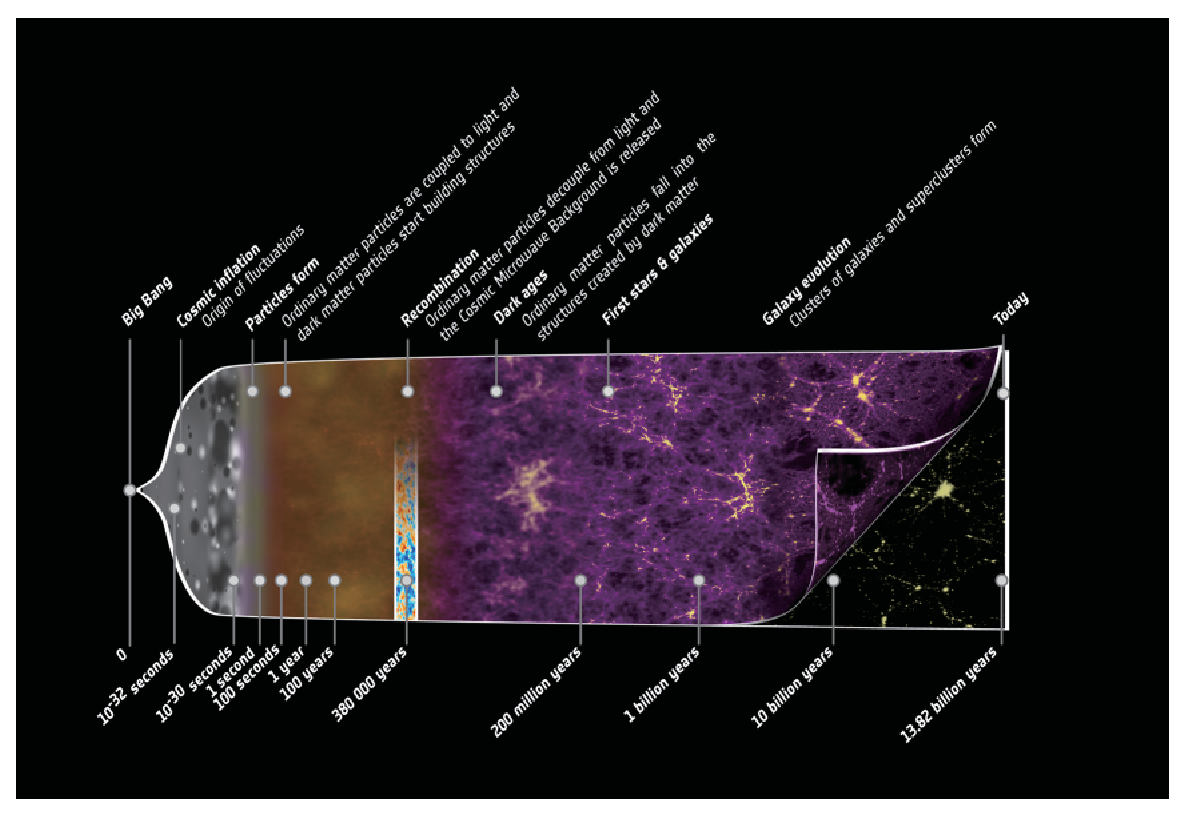
\includegraphics[width=0.8\linewidth]{cosmology/Planck_history_of_Universe_Crop_orig.eps} 
\caption{宇宙の構造進化の歴史(Planck web pageより)。}\label{fig:cosmo_history}
\end{center}
%\end{figure}
%%%%%%%%%%%%%%%%%%%%%%%%%%%%%%%%%%%%%%%%%%%%%%%%%%%%%%%%%%%%%%%%%%%%%%%%%%%%

%%%%%%%%%Figure%%%%%%%%%%%%%%%%%%%%%%%%%%%%%%%%%%%%%%%%%%%%%%%%%%%%%%%%%%%%%
%\begin{figure}[t]
 \begin{minipage}{0.6\hsize}
 \begin{center}
   \vspace{15pt}
   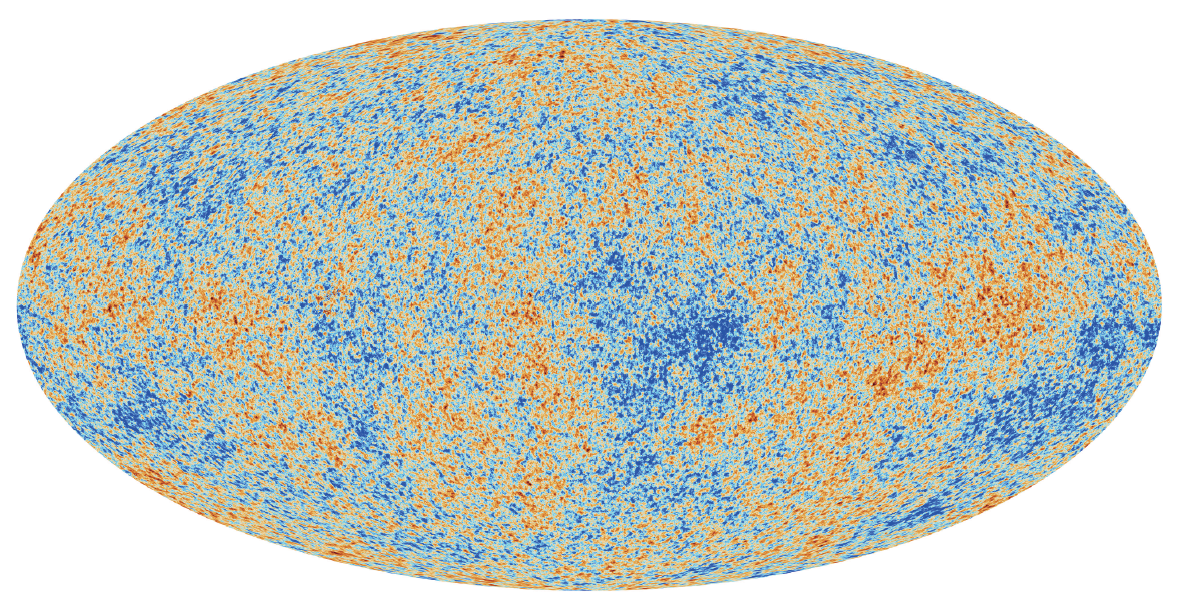
\includegraphics[width=0.7\linewidth]{cosmology/Planck_CMB_Mollweide_4k_2.eps} 
   \vspace{10pt}
   \caption{PlanckによるCMB温度揺らぎの全天マップ(Planck web pageより)}\label{fig:Planck_CMB}
 \end{center}
 \end{minipage}
 \begin{minipage}{0.4\hsize}
 \begin{center}
   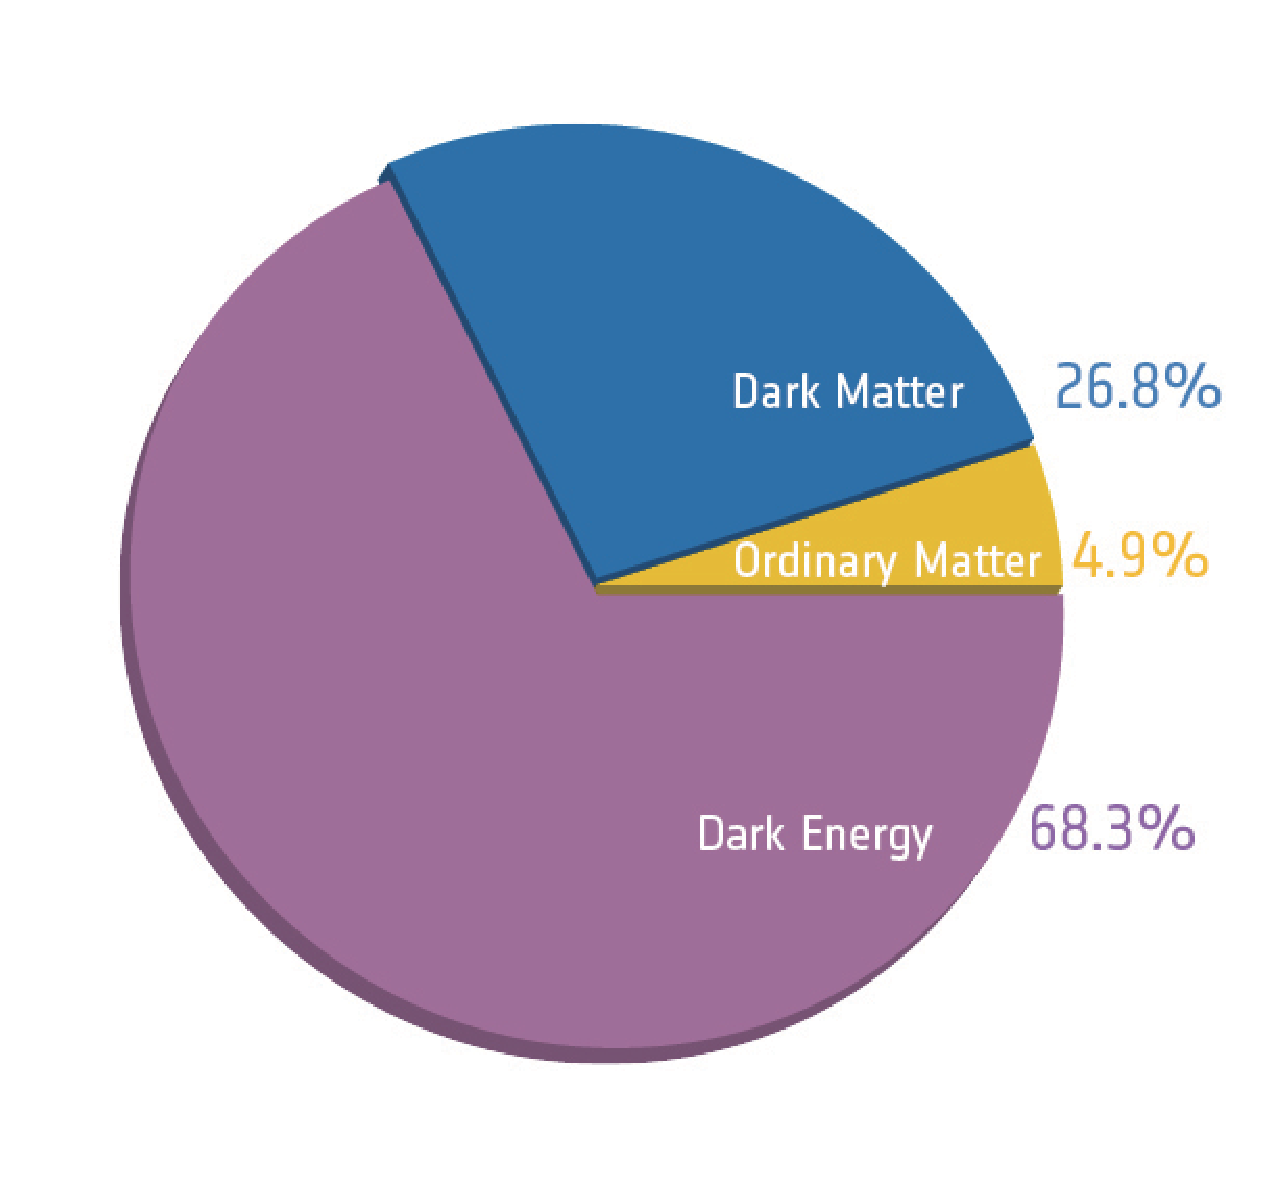
\includegraphics[width=0.8\linewidth]{cosmology/component_univ.eps} 
  \vspace{-15pt}
  \caption{宇宙の構成成分(Planck web pageより)。}\label{fig:component}  
 \end{center}
 \end{minipage}
\end{figure}
%%%%%%%%%%%%%%%%%%%%%%%%%%%%%%%%%%%%%%%%%%%%%%%%%%%%%%%%%%%%%%%%%%%%%%%%%%%%

宇宙論とは、宇宙全体やその内部に存在する構造物が、どのように形成されそして発展してきたのかについて、科学的手法を用いて理論的・観測的に解明していく学問である(図~\ref{fig:cosmo_history})。特に近年の観測技術の発達により、標準的な宇宙モデルはほぼ確立しており、それは次のようなものである。

まず、大局的なスケール(超銀河団を超えるスケール、約$100$Mpc以上)で宇宙を平均して見た場合、特別な場所は存在せず(一様性)、また特別な方向も存在しない(等方性)という一様等方宇宙モデルを採用している。現在のところ、このモデルが成り立っていないという確実な証拠は存在しない。さらに、宇宙内部の構成物についても、ビッグバン後約$38$万年頃に原子が形成され光が直進できるようになった時期の残光である宇宙マイクロ波背景放射(Cosmic Microwave Background radiation : CMB)の精密観測が行われたことにより(図\ref{fig:Planck_CMB})、このモデルの妥当性が確認されている。最新のCMB観測衛星Planck~\citep{Ade:2013zuv}の観測結果によると、通常の物質を構成するバリオンの量は、宇宙全体の約$5$\%程度に過ぎず、約$27$\%がほぼ重力相互作用しか行わない冷たい暗黒物質(cold dark matter)で構成され、さらに約$68$\% が宇宙の膨張を加速させる原因となる正体不明のエネルギー(暗黒エネルギー:dark energy)であるということが分かっている(図~\ref{fig:component})。またこのモデルでは一定の空間曲率が許されているが、CMBの観測からこの曲率は非常に小さく制限されており、この宇宙は平坦な宇宙であるということが判明している。典型的な宇宙論パラメータを表\ref{cosmological parameters1}, \ref{cosmological parameters2}に示す。

このように一様等方宇宙モデルは、観測を非常に良く説明するモデルであるが、そもそもなぜこのような条件の宇宙が生じたのかという疑問が生じてくる。その疑問に対し説明を与える最も有力なモデルが、宇宙初期における指数関数的急膨張(インフレーション)を仮定するモデルである。このインフレーションモデルでは、宇宙初期の光速を超える急膨張によって、当初因果関係を持っていた小さな領域を現在観測可能な範囲(宇宙の地平線)を超えて拡大することにより、非常に一様で等方な宇宙を実現することができる。またこの膨張によって、曲率は均されて小さくなり、非常に平坦な宇宙が実現する。さらにインフレーションモデルでは、インフレーションを生じさせる場としてインフラトンという場を仮定するが、その場の量子的な揺らぎから、銀河などの大規模構造の種となるわずかな密度揺らぎを生成することも可能にしている。

以上が現在標準的な宇宙モデルであるが、その上で今後解明を目指すべき重要な問題としては、次のようなものを挙げることができる:
(i) インフレーションモデルの検証、
(ii) 暗黒エネルギーの性質の解明及び修正重力理論の可能性の検証、
(iii) 暗黒物質の正体の特定。
以下で、これらの問題についての解説及びその観測的な制限について順に説明していく。

%\vspace{10pt}


%TTTTTTTTTTTTTTTTTTTTTTTTTTTTTTTTTTTTTTTTTTTTTTTTTTTTTTTTTTTTTTTTTTTTTTTTT%
\begin{center}
\begin{table}[t]
\caption{
標準的な宇宙論($\Lambda$CDM模型)におけるパラメータおよび$68\%$ C.L.エラー~\citep{Ade:2013zuv}。
}
\begin{center}
 \vspace{15pt}
\begin{tabular}{ccc} \hline \hline 
宇宙論パラメータ & 値 & 定義 \\ 
\hline 
$\Omega_{\rm b}h^2$ & $0.02214\pm 0.00024$ & 現在のバリオン密度\\
$\Omega_{\rm c}h^2$& $0.1187\pm 0.0017$ & 現在の冷たい暗黒物質密度\\
$\tau$ & $0.092\pm 0.013$ & 再電離によるトムソン散乱の光学的厚さ\\
$\ln (10^9 A_{\rm s})$ & $3.091\pm 0.025$ & 原始曲率揺らぎパワースペクトルの振幅\\
$n_{\rm s}$ & $0.9608\pm 0.0054$ & 原始曲率揺らぎパワースペクトルの冪指数\\
%\hline
$H_0=100h$ & $67.80\pm 0.77$ & 現在のハッブル定数 $[{\rm km}/{\rm s}/{\rm Mpc}]$\\
$\Omega_\Lambda$ & $0.692\pm 0.010$ & 現在の暗黒エネルギー密度\\
\hline
\hline 
\end{tabular}
\end{center}
\label{cosmological parameters1}
\end{table} 
\end{center}
%TTTTTTTTTTTTTTTTTTTTTTTTTTTTTTTTTTTTTTTTTTTTTTTTTTTTTTTTTTTTTTTTTTTTTTTTT%


%%%%%%%インフレーション関係%%%%%%%%%%%%%%%%%%%%%%%%%%%%%%%%%%%%%%%%%%%%%%%%%
\paragraph{(i) インフレーションモデルの検証}
%まず始めに、インフレーションモデルの検証方法について説明していく。
%
インフレーションモデルの検証において最も基本的な方法は、宇宙の密度揺らぎの測定である。これまで述べたように、インフラトンの量子揺らぎは最終的に密度揺らぎの起源となるが、この揺らぎはインフレーションのモデルの違いによって、特徴のある空間スケール依存性を示す。よって、その特徴を観測的に捉えることが、各インフレーションモデルを制限していく上で非常に有効な手段となる。

またインフレーションで生成される密度揺らぎはほぼガウス分布に従うことが知られているが、各モデルによってガウス分布からの微小なズレの程度(原始非ガウス性)が異なっている。そのため、この原始非ガウス性を測定することもこのモデルを制限する非常に有効な方法の一つである。
インフレーションの一般的なモデルでは、確率分布として様々な非ガウス性を持つ原始揺らぎを生成しうる。
原始揺らぎのガウス分布からのズレを表す最も便利な方法として、重力ポテンシャル$\Phi$が
ランダムガウス場$\phi$の線形項と2次の補正の和で
\begin{align}
	\Phi =\phi +f_{\rm NL}\left(\phi^2 -\langle\phi^2\rangle\right)
	\,.\label{eq:fNL def}
\end{align}
と書かれる場合を考える。
ここで、$f_{\rm NL}$は非線形パラメータと呼ばれる定数であり、$\langle\cdots\rangle$はアンサンブル平均を表す。
この場合、その統計的性質はパワースペクトルだけでは記述できず、
バイスペクトルのような高次のモーメントが必要になる。
異なるインフレーション模型は異なるバイスペクトルの形を予言することから、この探求により
インフレーションの物理について深い理解を得ることができる。
これまでCMBの精密な観測により、インフレーションの物理に対して精度よく制限がなされている(\ref{cosmology.s1.ss2}節)。
特に、Planck衛星による観測~\citep{Ade:2013ydc}によれば、非線形パラメータは$f_{\rm NL}=2.7\pm 5.8$となる制限が得られており、$f_{\rm NL}>10$となるような比較的大きな非ガウス性を生成するモデルや、モデル内のパラメータを制限することに成功している。
後述するように、銀河サーベイからも原始非ガウス性を探査することができる。
しかし、未知の系統誤差の影響により、現在までの制限は$\sigma (f_{\rm NL})\approx 50$程度に留まっている\citep{Ho:2013lda,Giannantonio:2013uqa}。

加えて、インフレーションの検証に非常に重要な観測として、インフレーション起源の原始重力波の観測が挙げられる。この原始重力波は、インフレーション中に重力場の量子揺らぎから生成されたものであり、その振幅はインフレーションのエネルギースケールと直接関係づくことが知られている。そのため、もしこの原始重力波を観測できれば、地上の加速器実験ではとても到達できない、
%ほど大きなエネルギーのスケールである
インフレーションの生じた超高エネルギーの物理の情報を直接知ることができるのである。

%現在、Planck衛星によるCMB温度揺らぎの観測から揺らぎのスケール依存性や原始重力波の強い制限が得られており~\citep{Ade:2013uln}、今後はより精密なCMB偏光の観測や、広い範囲の銀河サーベイ、または再電離の時期の水素が発する21cm線の観測によって、更に高い精度でインフレーションモデルの検証が行えると期待される。
%制限が得られると期待されている。
%また
%原始重力波については、
%その原始重力波の振幅が比較的大きなものであれば、
%将来の宇宙重力波干渉計を用いれば、原始重力波のスペクトルを直接観測できる可能性さえ存在している。


%TTTTTTTTTTTTTTTTTTTTTTTTTTTTTTTTTTTTTTTTTTTTTTTTTTTTTTTTTTTTTTTTTTTTTTTTT%
\begin{center}
\begin{table}[t]
\caption{
標準宇宙論に非標準的な$1$パラメータを加えた場合の$95\%$ C.L.エラー~\citep{Ade:2013zuv}。
}
\begin{center}
% \vspace{15pt}
\begin{tabular}{ccc} \hline \hline 
宇宙論パラメータ & 値 & 定義 \\ 
\hline 
$r$ & $<0.111$ & 原始重力波揺らぎパワースペクトルの振幅\\
$w$ & $-1.13
   \begin{array}{l}
      +0.23 \\
      -0.25
    \end{array}$
& 暗黒エネルギーの状態方程式\\
$\Omega_{\rm K}$ & $-0.0005
   \begin{array}{l}
      +0.0065 \\
      -0.0066
    \end{array}$
& 現在の空間曲率密度\\
$\frac{{\rm d}n_{\rm s}}{{\rm d}\ln k}$ & $-0.014
   \begin{array}{l}
      +0.016 \\
      -0.017
    \end{array}$
& 原始曲率揺らぎパワースペクトルの冪指数のランニング \\
$\sum m_\nu\,[{\rm eV}]$ & $<0.230$ & ニュートリノ質量和 \\
$N_{\rm eff}$ & $3.30
   \begin{array}{l}
      +0.54 \\
      -0.51
    \end{array}$
& ニュートリノの実効的な自由度の数\\
\hline
\hline 
\end{tabular}
\end{center}
\label{cosmological parameters2}
\end{table} 
\end{center}
%TTTTTTTTTTTTTTTTTTTTTTTTTTTTTTTTTTTTTTTTTTTTTTTTTTTTTTTTTTTTTTTTTTTTTTTTT%
%%%%%%%暗黒エネルギー関係%%%%%%%%%%%%%%%%%%%%%%%%%%%%%%%%%%%%%%%%%%%%%%%%%%%
\paragraph{(ii) 暗黒エネルギーの性質の解明及び修正重力理論の可能性の検証}
%%%%%%%%%%%%%%%%%%%%%%%%%%%%%%%%%%%%%%%%%%%%%%%%%%%%%%%%%%%%%%%%%%%%%%%%%%%%
%次に暗黒エネルギーの問題とについて説明していく。
%
宇宙の加速膨張の原因となるエネルギーを一般に暗黒エネルギーと呼ぶが、その存在が決定的になったのは、1990年代末のIa型超新星を用いた宇宙膨張の観測以降である~\citep{Riess:1998cb,Perlmutter:1998np}。
それらの観測により、観測された超新星の見かけの光度が、減速膨張宇宙の場合と比べて暗いという事実が発見された。
これは同じ後退速度で運動する、もしくは同じ赤方偏移を示す超新星までの距離が減速しているときに比べて相対的に大きいことを意味する。
このことから、宇宙が加速膨張しているということが判明した。

この暗黒エネルギーの最も単純な候補は、時間変化しない一定密度のエネルギー(宇宙定数)であり、そのようなエネルギーとして量子場の真空のエネルギーが考えられている。しかし、この場合、理論的に推定される真空のエネルギー密度は、観測された暗黒エネルギーの密度より120桁以上も大きな値となってしまい、この様な微小な真空のエネルギーを自然に説明することは非常に難しい。

そのため、加速膨張がそのような真空のエネルギー起源ではなく、何等かの加速膨張の原因となる新しい場を導入するモデル(クインテッセンス等)も数多く提案されている。
さらに一般相対性理論自体を修正することにより加速膨張を説明するというアプローチも存在し、それらは一般に修正重力理論と呼ばれている。
一般相対論は、重力の効果が弱い実験室や太陽系スケールでは既に非常に厳しい制限がなされているが、重力が
重要になりえる宇宙論的な大スケールでは大きくずれている可能性がある。
観測的な制限を回避しうる模型がいくつか提案されており、その中で有名な模型としては
$f(R)$重力理論、DGPブレーンワールド模型、スカラーテンソル理論、有質量重力理論等がある。
また一様等方宇宙モデルを修正した非一様宇宙モデルによって観測を説明するという方向も考えられている。

これら宇宙定数以外のモデルの場合、暗黒エネルギーの密度は一般に時間変化することから、この影響を観測することで
宇宙定数の場合と区別することが可能である。
特に、暗黒エネルギーのエネルギー密度$\rho$および圧力$P$を用いて作られる状態方程式パラメータ
\begin{align}
	w=\frac{P}{\rho}\,,
	\label{eq:DE EOS def}
\end{align}
を検証することが行われている。
多くの場合、$w$を定数として扱い制限を行ってきた(表\ref{cosmological parameters2}参照)。
状態方程式パラメータの時間進化を特徴付ける代表的な方法として、
\begin{align}
	w(z)=w_0+w_a\,\frac{z}{1+z}
	\,,
	\label{eq:DE EOS}
\end{align}
となる二つの定数$w_0,w_a$を導入する手法も行われている。
宇宙項が暗黒エネルギーだった場合、その状態方程式$w$は厳密に$-1$となるため、$(w_0,w_a)=(-1,0)$に対応する。
修正重力理論の場合には、一般的に$w$が時間進化することから$w_a$が非自明な値をとり得る。
これらは、宇宙膨張が密度揺らぎの成長に与える影響、特にバリオン音響振動(Baryon Acoustic Oscillation; BAO)
および赤方偏移空間歪み(Redshift Space Distortion; RSD)と呼ばれる効果を銀河の赤方偏移サーベイによって
観測することで知ることができる(\ref{cosmology.s1.ss1-2}節)。
現在の所、CMBと超新星の観測及びBAOの観測を組み合わせることにより、
暗黒エネルギーの状態方程式パラメータに対し
$w_0=-1.04
   \begin{array}{l}
      +0.72 \\
      -0.69
	\end{array}$
および$w_a<1.32$なる制限が得られているが、
有意な宇宙定数からのズレは今のところ観測されてはいない~\citep{Ade:2013zuv}。そのため今後は、より広い赤方偏移の観測を行うことにより、本当に暗黒エネルギーが宇宙定数であるのか、それとも厳密な宇宙定数の場合とは違いがあるのかについて、より精密に測定していくことが宇宙論における重要な目標となっている。


%%%%%%%暗黒物質%%%%%%%%%%%%%%%%%%%%%%%%%%%%%%%%%%%%%%%%%%%%%%%%%%%%%%%%%%%%
\paragraph{(iii) 暗黒物質の正体の特定}
%%%%%%%%%%%%%%%%%%%%%%%%%%%%%%%%%%%%%%%%%%%%%%%%%%%%%%%%%%%%%%%%%%%%%%%%%%%%
最後に正体は不明ながらも、現在その存在はほぼ確実視されている冷たい暗黒物質とその観測可能性について説明していく。まず冷たい暗黒物質とは、運動エネルギーが質量エネルギーより小さい暗黒物質のことであり、逆に運動エネルギーが大きな暗黒物質のことを熱い暗黒物質と呼ぶ。熱い暗黒物質は自身の自由運動のために、小スケールの密度揺らぎが均されて消されてしまい、観測されている密度揺らぎを正しく説明することができない。そのため、暗黒物質は冷たい暗黒物質がほとんどを占めていると考えられている。

通常の物質とはほぼ相互作用せず、重力によってのみ相互作用する暗黒物質の存在は、1930年代には銀河団の解析から既に示唆されており、また1970年代には銀河の回転曲線の観測から銀河は光を放っている円盤部分よりも質量を担う領域が大きく広がっており、むしろそちらが銀河の質量の大部分を占めているということが判明していた。

そのため、その正体を突き止めることが現在の宇宙論における目標の一つとなっている。暗黒物質の正体を探る方法としては、暗黒物質がわずかに行う可能性のある通常の物質との相互作用を検出する直接検出実験
や、暗黒物質が対消滅や崩壊をする際に生成されるガンマ線や高エネルギーの粒子を観測する間接検出実験が多数行われている状況である。
また、現在においては、銀河サーベイにおける弱重力レンズ効果(\ref{cosmology.s1.ss1-2}節)を用いることで、
前景にある暗黒物質量を推定することができることから暗黒物質の空間分布を観測から探ることも広く行われている。

\subsection{宇宙論的観測手法}\label{cosmology.s1.ss1-2}

この節では、銀河サーベイを用いた代表的な観測手法についていくつか簡単に触れておくことにする。
まず既に言及したBAOについて説明する。
バリオン音響振動とは宇宙の再結合以前に光子とバリオンがトムソン散乱とクーロン相互作用を
通じて混合流体として存在していた時期の音波振動と、再結合後に音波振動が光子から
脱結合したバリオンとダークマターの重力相互作用を通じて宇宙大規模構造に反映された振動パターンを指す。
後者のBAO振動パターンのスケールは、音響ホライズンと呼ばれる混合流体の音波が再結合までの宇宙年齢をかけて進む距離
$r_{\rm s}$で与えられ、密度揺らぎの相関関数に特徴的なピークを残す効果として観測される(図~\ref{fig:BOSS_BAO})。
再結合時から現在に至るまで不変であるため宇宙の大規模構造を測定する際の距離指標として使うことが可能である。
そのため、宇宙の大規模構造の観測でBAOを検出することによって宇宙の空間的な幾何学や膨張の履歴を小さな系統誤差で
導くことが可能で、ダークエネルギーの物理的性質、一般相対論的な重力理論の検証などの宇宙に関する物理学の基本的問
題を調べる手段となりうる。


%%%%%%%%%Figure%%%%%%%%%%%%%%%%%%%%%%%%%%%%%%%%%%%%%%%%%%%%%%%%%%%%%%%%%%%%%
\begin{figure}[t]
 \begin{minipage}{0.5\hsize}
 \begin{center}
   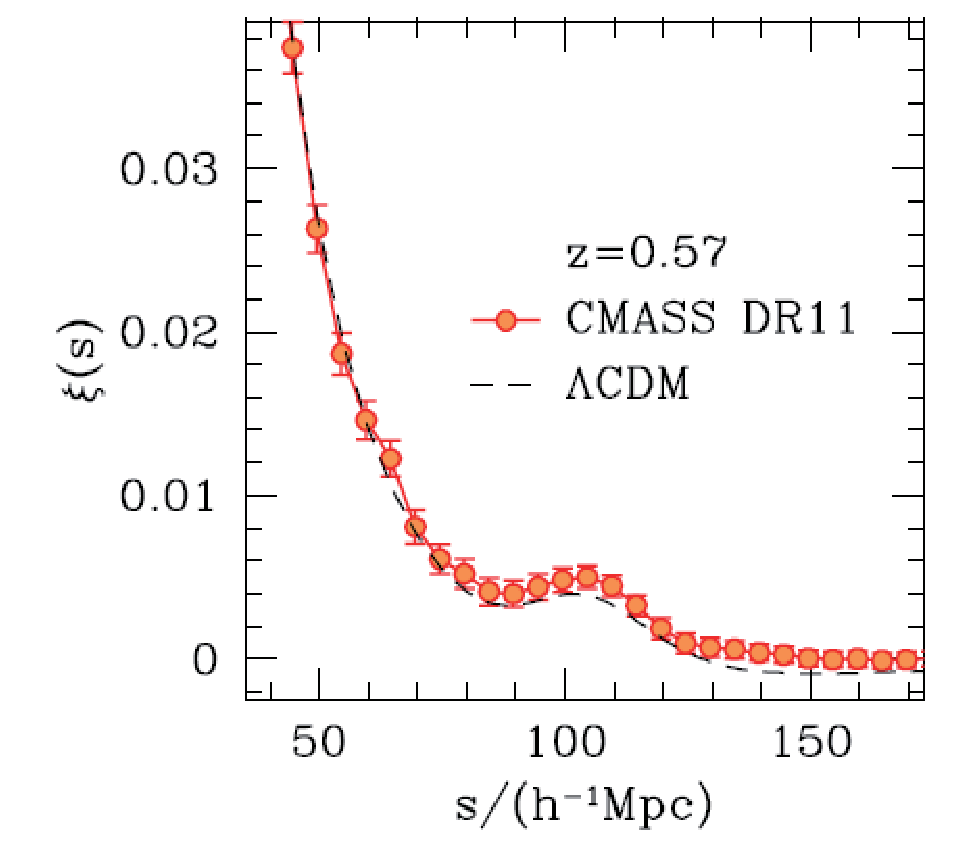
\includegraphics[width=0.95\linewidth]{cosmology/SDSS_BOSS_DR11_BAO.eps}   
   \caption{SDSS-III BOSSサーベイ(DR11)による角度平均した銀河の相関関数$\xi$~\citep{Sanchez:2013tga}。
            横軸は距離のスケールを表し、$100{\rm h}^{-1}{\rm Mpc}$付近にバリオン音響振動による
            ピークが見える。なお$\Lambda$CDMとは標準宇宙モデルのことである。}\label{fig:BOSS_BAO}
 \end{center}
 \end{minipage}
 \hspace{5pt}
 \begin{minipage}{0.5\hsize}
 \begin{center}\vspace{-10pt}
   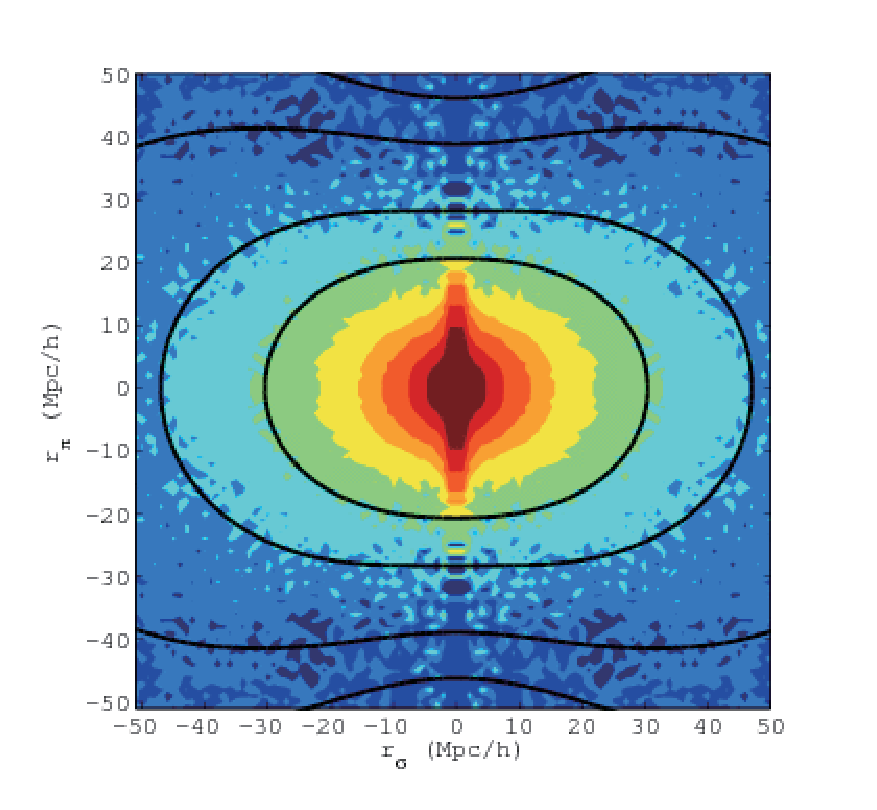
\includegraphics[width=0.95\linewidth]{cosmology/butterfly_colour_smallerscales.eps} 
   %\vspace{10pt}
   \caption{SDSS-III BOSSサーベイ(DR9)による、銀河の相関関数(赤いほど相関関数が大きい)~\citep{Reid:2012sw}。
           縦軸は視線方向、横軸は天球面上での距離スケールである。
           この縦方向と横方向における歪みが、赤方偏移空間歪みである。
           }\label{fig:BOSS_RSD}  
 \end{center}
 \end{minipage}
\end{figure}
%%%%%%%%%%%%%%%%%%%%%%%%%%%%%%%%%%%%%%%%%%%%%%%%%%%%%%%%%%%%%%%%%%%%%%%%%%%%

加えて、銀河の相関関数の非等方性として観測されるRSDも非常に有用な手法として
盛んに利用されている。赤方偏移空間歪みとは、個々の銀河の固有速度によって生じた赤方偏移による効果で、
たとえ実空間における銀河の分布が等方であっても、実際に観測される赤方偏移空間上では非等方な揺らぎとなってしまうことから発生する(図~\ref{fig:BOSS_RSD})。この固有速度の影響は、密度揺らぎの成長率と関係づくため、その成長に対する暗黒エネルギーの影響を調べることに利用することができる。

最後に、弱重力レンズ効果を利用した方法を説明する。
重力レンズ効果は、サーベイ対象の銀河からの光が経路上の物質による重力によって経路が直線からズレることで発生する。
その中でも弱重力レンズ効果とは、物質の重力によって発生する重力レンズ効果の内、
像の歪みが小さいために単独の観測対象を見ているだけでは
その影響が分からないもののことを呼ぶ。
したがってこの弱重力レンズ効果は、多数の観測対象を統計的に処理することで、
初めてその効果を測定することが可能となる。
%
この弱重力レンズ効果は宇宙の物質分布つまり密度揺らぎの情報を保持しており、
暗黒物質のエネルギー密度や暗黒エネルギーが密度揺らぎの成長に与える影響などについて、
詳細に調べるために利用することができる。

%%%%%%%%%%%%%%%%%%%%%%%%%%%%%%%%%%%%%%%%%%%%%%%%%%%
\vspace{15pt}

%%%%%%%まとめ%%%%%%%%%%%%%%%%%%%%%%%%%%%%%%%%%%%%%%

以上の様に、宇宙論における未解決問題であるインフレーションの検証、暗黒エネルギーおよび暗黒物質の正体の特定に向け、
様々な観測手法を用いることで宇宙論研究が行われている。
ここまで挙げた観測手法による宇宙論は、これまではほとんど光赤外観測によって推進されてきた。
将来観測(電波以外の波長については次節参照)により、これらの理解は格段に進歩することが予想される。
しかし、今後はSKAが登場することで電波によりこれらの観測を行うことが可能になり、電波観測によるこれまでにない規模・精度の
宇宙論を行うことができるようになる。
これにより、理論・観測両方面における宇宙論分野の更なる発展が期待される。

\subsection{他波長の将来計画}\label{cosmology.s1.ss2}

\subsubsection{マイクロ波背景放射}
これまで、COBEによる黒体輻射スペクトルの精密測定、地平線を超えた温度揺らぎの検出に始まり、DASIによるEモード偏光の検出~\citep{Kovac:2002fg}, WMAP衛星~\citep{Bennett:2012zja}, Planck衛星~\citep{Ade:2013zuv}による温度揺らぎの精密観測による宇宙論パラメタの決定、最近ではSPTPol~\citep{Hanson:2013hsb}, PolarBear~\citep{Ade:2013hjl}両実験による重力レンズ由来のBモード偏光の検出、さらにはBICEP2実験による重力波由来のBモード偏光の検出~\citep{Ade:2014xna}と、CMB実験はここ10年で急速な進展を遂げている。2014年末のPlanck衛星の偏光揺らぎの観測結果の発表をもって線形段階の密度揺らぎに由来するCMB温度揺らぎ・偏光揺らぎの観測は一段落を迎えることになる。%このPLANCKの結果次第でもあるが、その後の
今後のCMBの観測的研究の方向は大きく以下の4つが考えられる。
(観測計画リストは\ref{table:CMB future plan}参照)


\paragraph{重力波由来のBモード偏光スペクトルの詳細観測}
BICEP2によって報告されたBモード偏光検出については主要な観測が$1$周波数帯のみでしか行われておらず、前景放射のもれこみの問題が指摘されている\citep{Flauger:2014qra,Mortonson:2014bja}。Planckの複数の周波数帯による偏光観測により前景放射の情報が得られることが期待されているが~\citep{Adam:2014bub}、もしBICEP2の検出したシグナルが前景放射によるものだった場合、これまで以上に感度を上げた観測が必要となる。また、インフレーション由来の重力波であることを結論付けるためには、再イオン化によるバンプや整合性条件のチェックなど、広いスケールに渡ってスペクトルを観測する必要があり(例えば\citep{Dodelson:2014exa})、大角度スケールの観測に特化した地上観測や、衛星観測が必要になる。


\paragraph{重力レンズ由来のBモード偏光観測}
CMB弱重力レンズ効果は、宇宙晴れ上がり時の温度・偏光揺らぎの分布が、手前にある大規模構造による重力ポテンシャルによって歪められることによって発生する。特に密度揺らぎ起源であるEモードがレンズ効果によりBモードに変換されるが、このBモードは小スケールで他からのシグナルを卓越するため、重力ポテンシャルを再構築するのに適している\citep{Okamoto:2003zw,Hirata:2003ka}。重力レンズ効果によって推定される大規模構造は宇宙に存在する物質と重力の情報を含むため、例えばニュートリノ質量の精密測定や重力理論の検証などに用いることができる。


\paragraph{スニヤエフ・ゼルドビッチ(Sunyaev-Zel'dovich; SZ)効果}
大規模構造に付随する高温プラズマ(主に銀河団)はCMB光子を電子の熱運動によって逆コンプトン散乱することにより、CMBの黒体放射を歪ませる(熱的SZ)。この歪みの大きさは高温ガスの内部エネルギーに比例するため、重力ポテンシャルすなわち銀河団の質量のよい指標になる。また、この歪みは高周波側では温度の上昇、低周波側では温度の下降として観測され、温度揺らぎの観測からも検出することができる。一方、宇宙の再イオン化期に生成されるイオン化領域によるコンプトン散乱はその領域の特異速度に依存したドップラー効果により新たな温度揺らぎを生み出し(動的SZ)この効果を観測することにより、宇宙再イオン化期の情報(再イオン化開始時刻や時間など)を得ることが期待できる。


\paragraph{スペクトル歪みの詳細観測}
角度揺らぎとは別の方向性として、CMBのプランク分布からのずれの詳細な観測が計画・議論されている。宇宙初期における熱浴への熱流入は時期によって$\mu$歪み・$y$歪みを引き起こし、この歪みを詳細に観測することにより初期宇宙での物理過程を調べることができる。物理過程には、スニヤエフ・ゼルドビッチ効果の他に例えば粘性散逸による加熱や、ダークマターの崩壊、初期磁場の散逸などがある~\citep{Tashiro:2014pga}。


\begin{table}
 \centering
 \begin{tabular}{c|l|cccc}\hline\hline
  種類 &  \hspace{2zw}計画名\hspace{2zw} & 重力波 & 重力レンズ & \hspace{0.5zw}SZ\hspace{0.5zw} & スペクトル歪み \\\hline
  \multirow{4}{*}{人工衛星}
  & COrE+ & \checkmark & \checkmark & \checkmark \\\cline{2-6}
  & EPIC-IM & \checkmark & \checkmark & \checkmark & \\\cline{2-6}
  & LiteBIRD & \checkmark & & & \\\cline{2-6}
  & PIXIE & \checkmark & & & \checkmark \\\hline
  \multirow{5}{*}{バルーン}
  & EBEX* & \multirow{2}{*}{\checkmark} & & & \\
  & EBEX6K & & & & \\\cline{2-6}
  & LSPE & \checkmark & & & \\\cline{2-6} 
  & PIPER* & \checkmark & & & \\\cline{2-6} 
  & \textsc{Spider}* & \checkmark & & & \\\hline
  \multirow{17}{*}{地上}
  & ABS* & \checkmark & & & \\\cline{2-6}
  & ACTPol* & \multirow{2}{*}{\checkmark} & \multirow{2}{*}{\checkmark} & \multirow{2}{*}{\checkmark} & \\
  & AdvACTPol* & & & & \\\cline{2-6}
  & B-Machine* & \checkmark & & & \\\cline{2-6}
  & CLASS* & \checkmark & & & \\\cline{2-6}
  & GLP & \checkmark & & & \\\cline{2-6}
  & GroundBIRD & \checkmark & & & \\\cline{2-6}
  & Keck array* & \multirow{2}{*}{\checkmark} & & & \\
  & BICEP3* & & & & \\\cline{2-6}
  & MuSE & \checkmark & & & \\\cline{2-6}
  & \textsc{Polarbear}* & \multirow{3}{*}{\checkmark} & \multirow{3}{*}{\checkmark} & & \\
  & \textsc{Polarbear-2}* & & & & \\
  & Simons Array* & & & & \\\cline{2-6}
  & QUBIC* & \checkmark & & & \\\cline{2-6}
  & QUIJOTE* & \checkmark & & & \\\cline{2-6}
  & SPTpol* & \multirow{2}{*}{\checkmark} & \multirow{2}{*}{\checkmark} & \multirow{2}{*}{\checkmark} & \\
  & SPT-3G* & & & & \\\hline\hline
\end{tabular}
\caption{各CMB観測に関する星取表。*印は観測予定または観測中のもの。
ただし、重力波に関しては各実験が「low-$\ell$をターゲットにしている」「low-$\ell$を観測出来る」と明記しているもの、
重力レンズに関しては独自に重力レンズ角度パワースペクトルを評価できるだけチェックマーク( $\checkmark$ )を付けている。
監修:茅根氏}
\label{table:CMB future plan}
\end{table}



\subsubsection{光赤外}

宇宙論を主なターゲットにした光赤外サーベイは数多く計画されている。主要なアプローチとしては、弱い重力レンズの統計、銀河などの天体の空間分布の相関関数によるバリオン音響振動や赤方偏移空間歪みの効果、Ia型超新星爆発などが用いられる。観測装置としては地上望遠鏡と宇宙望遠鏡を使う方法に大別される。宇宙望遠鏡は大気の窓を越えてしか観測できない中間・遠赤外線の場合には地上では難しい高空間分解能や高感度を達成しうるという利点はあるが、一方で大口径の望遠鏡や超広視野の撮像装置、大掛かりな分光装置などを宇宙に打ち上げるのは非現実的であるので地上の大型望遠鏡も相補的な重要な役割を果たす。サーベイ観測には撮像サーベイと分光サーベイがあり前者は主に重力レンズやIa型超新星爆発、後者は主に銀河相関関数を用いた宇宙論を目指しこれらも相補的である。

撮像サーベイで$2020$年頃までの主力となるのは、すばる$8$m望遠鏡を用いた日本の Hyper Suprime-Cam (HSC) サーベイとアメリカが主導するチリの4m望遠鏡を使ったDark Energy Survey (DES) である。HSCは$1400$~deg$^2$の領域を$r\sim 26$等の深さで観測するのに対して、DESは$5000$~deg$^2$の領域を$r\sim 25$等とやや浅く観測していく。両者ともサーベイ観測を開始したばかりであり$5$年かけてサーベイを行っていく。

$2020$年以降に主力となる次世代サーベイはEuclid (Europian Space Agency (ESA))、WFIRST-AFTA (NASA)、Large Synoptic Survey Telescope (LSST; アメリカ) である。EuclidとWFIRST-AFTAは宇宙望遠鏡であり、地上からは感度が悪い近赤外での観測に重点がおかれている。また宇宙での観測は高空間分解能の画像が容易に得られるので弱い重力レンズで必須となる銀河の精確な形状測定の上で多くの利点がある。実際にEuclidは$15000$~deg$^2$の$r\sim25 $等の撮像データを用いた重力レンズ宇宙論を主なターゲットとしている。WFIRST-AFTAは多目的宇宙望遠鏡ではあるが$2000$~deg$^2$程度の領域をEuclidよりも深く観測し弱い重力レンズなどに用いることが予定されている。また遠方のIa型超新星爆発を狙った超新星サーベイも計画されている。LSSTはチリに$8$mの専用望遠鏡を設置しサーベイ観測を行う。LSSTは南天の$20000$~deg$^2$の領域を観測するが、その大きな特長としては時間変動の大規模なサーベイを行う点にある。具体的にはLSSTは一回の撮像で$r\sim 24$等の浅い観測を行い、この観測を数日おきに何度も繰り返し、最終的には同じ空の領域を何百回と観測し最終的な撮像データは$r\sim 27$等に達すると見積もられている。これにより時間変動する天体、例えば超新星爆発やクエーサーといった天体を全天規模で大量に発見することができ、時間変動天体に対する理解が圧倒的に進むであろうと期待されている。これに関しては東京大学で計画されているThe University of Tokyo Atacama Observatory (TAO)も重要な寄与をすると期待される。この大規模な時間変動を利用した宇宙論研究、たとえばIa型超新星爆発の統計解析や強い重力レンズの時間の遅れの研究などで大きな進歩が期待できる。

一方将来の分光サーベイとしては、Sloan Digital Sky Surveyの第四期サーベイの一つ Extended Baryon Oscillation Spectroscopic Survey (eBOSS; $2014$年開始)、すばる望遠鏡に取り付けられる予定の多天体分光器 Prime Focas Spectrograph (PFS; $2017$年頃以降)などがあり、$2020$年以降には地上4m望遠鏡に多天体分光器を取り付けるアメリカの計画 Dark Energy Spectroscopic Instrument (DESI) もある。またEuclidとWFIRST-AFTAの宇宙望遠鏡にもスリットレス分光機能が搭載され分光サーベイ観測を行う予定である。これらの分光サーベイの一番のターゲットはバリオン音響振動の観測による角径距離とハッブルパラメータの精密測定であり、これら将来計画により$0<z<3$の範囲で距離を1\%以下で測定しダークエネルギーの状態方程式に厳しい制限をつけることを目指す。

またこれらサーベイ観測と並んで、地上に$30$m級の大型望遠鏡を作る動きもある。アメリカや日本が主導する Thirty Meter Telescope (TMT)もその一つであり、ハワイに$30$m望遠鏡に設置し$2021$年稼働開始を目指している。ヨーロッパが主導するチリに$39$m望遠鏡を設置する European Extremely Large Telescope (E-ELT)、アメリカなどの同じくチリに$22$m望遠鏡を設置するGiant Magellan Telescope (GMT) も同時期の$2020$年頃の稼働を目指している。これらの大型望遠鏡は、暗い遠方銀河の分光観測による測光的赤方偏移の較正、遠方超新星爆発や強い重力レンズなどの宇宙論的に重要な天体の分光や補償光学を用いた高空間分解能撮像などの場面で活躍すると期待され、宇宙論研究にやはり重要な役割を果たす。



\subsubsection{X線}
X線観測による宇宙論の研究では、銀河団・銀河群の探査を行い、光赤外の観測による重力レンズ効果・電波観測によるSZ効果などから較正を行った推定質量を用いて銀河団・銀河群の質量関数と理論的なダークマターハローの質量関数を比較することで、宇宙論パラメータ・原始非ガウス性・重力理論などに制限を課すことが行われている。X線観測衛星のミッションは大きく分けて、銀河団・銀河群の大規模なカタログを作るsurvey型のミッションと、個々の銀河団を詳しく調べて推定質量の較正に役立てるobservatory型のミッションに分けられる。SKAが運用されるまでの今後$10$年間に計画されているX線観測衛星計画で、宇宙論的な文脈での研究が中心的なサイエンスを占めるものを以下に列挙する。
\begin{itemize}
\item ASTRO-H (日本・observatory型)\\
$2015$年秋に打ち上げ予定の日本のX線観測衛星で、世界で最初のTranslation Edge Sensor (TES)カロリメータを用いたX線分光装置 Soft X-ray Spectrograph (SXS) とCCDカメラSoft X-ray Imager (SXI) を用いた銀河団とその外縁部のX線観測が特徴的。
\item eROSITA on Spektr-RG (Russia, Germany・survey型)\\
ロシアとドイツが共同開発するSpektr-RGというX線観測衛星の観測装置の一つ。2014年Q3に打ち上げ予定だったが2015年に延期。有効面積の大きなX線望遠鏡とX線CCDの組み合わせで、X線での全天サーベイを行い銀河団とAGNのカタログを作成する予定。
\item DIOS (日本・observatory型)\\
ダークバリオンの大半を占めると考えられるWarm-Hot Intergalactic Medium (WHIM) 探査に特化したX線観測衛星。Diffuse Intergalactic Oxygen Surveyorの略。JAXA/ISASのイプシロンロケットを用いた小型科学衛星シリーズでの打ち上げを検討中。ASTRO-Hの$200$倍以上という非常に大きなグラプス(望遠鏡の有効面積と視野の積)を持つX線望遠鏡、TESカロリメータを用いた高いエネルギー分解能(5eV以下)のX線分光装置が特徴で$2020$年ごろの打ち上げを予定。
\item ATHENA (ESA)\\
ESAが計画中のX線観測衛星で$2028$年打ち上げ予定。eROSITAの更に$10$倍以上の有効面積を持つWide Field Imager (WFI)とTESカロリメータを用いた高いエネルギー分解能をもつX線分光器X-ray Integral Field Unit (X-IFU)を搭載し、これまでにない深いX線観測を行うことが可能になる。銀河団に関しては、赤方偏移が$1$を超える宇宙での銀河団や銀河群を内部構造も含めて観測する。また、再電離期程度の遠方宇宙までの銀河中心ブラックホールを観測することで、巨大ブラックホールの成長を理解することを目指している。
\end{itemize}




\subsection{SKA pathfinderによる宇宙論}\label{cosmology.s1.ss3}

以下、SKAのpathfinderによる宇宙論に関連したサーベイ計画をまとめておく。

\subsubsection{continuum survey}
\begin{itemize}
\item ASKAP EMU\\
正式名称はEvolutionary Map of the Universeで全天の75\%を$10~\mu{\rm Jy/beam~rms}$の感度、10-15 arcsecの角度分解能でサーベイし、約7千万個の銀河を観測する。$z=1$までのstar forming galaxyを観測できると期待されている。周波数帯は700-1800 MHz。
\item WODAN\\
正式名称はWesterbork Observations of the Deep APERTIF Northern-Skyで、WSRT (Westerbork Synthesis Radio Telescope)に配備されたphased array feed受信機であるAPERTIFを用いたサーベイである。ASKAPで観測できない全天の25\%の領域を$10~\mu{\rm Jy/beam~rms}$の感度、15 arcsecの角度分解能で観測する。
\item MeerKAT MIGHTEE\\
正式名称はMeerKAT International GigaHertz Tiered Extragalactic Exploration Survey。1.4 GHzでASKAP EMUやWODANに比べて狭い領域を深く観測する。
\item LOFAR\\
30-80 MHzと110-240 MHzの低周波で観測する。Tier 1, Tier 2, Tier 3の3つのサーベイフェイズがある。
\end{itemize}

\subsubsection{HI survey}

\begin{itemize}
\item ASKAP WALLABY\\
正式名称はWidefield ASKAP L-Band Legacy All-Sky Blind Surveyで全天の75\%を観測し$z=0.26$までの銀河を$500,000$個観測できる見込み。
\end{itemize}



\section{国際SKAのサイエンス}\label{cosmology.s2}

%%%%%%%%%%%%%%%%%%%%%%%%%%%%%%%%%%%%%%%%%%%%%%%%%%%%%%%%%%%%%%%%%%%%%%%%%%
\subsection{SKAによる宇宙論サーベイ}\label{cosmology.s2.ss0}
%%%%%%%%%%%%%%%%%%%%%%%%%%%%%%%%%%%%%%%%%%%%%%%%%%%%%%%%%%%%%%%%%%%%%%%%%%

SKAでは、これまでにない十分大きい体積、つまり十分多数のモードを観測することで、
CMBによる精密探査を超えた宇宙論の新しいフロンティアに到達することができる。
SKAはPhase-2が建造されたときには$\sim 10^9$個もの莫大な数の銀河を探査しうることから、
宇宙論における究極のサーベイ(``Billion galaxy survey'')として期待されている。
この節では以下、SKA Phase-1 (SKA1)およびPhase-2 (SKA2)における宇宙論サーベイについて
まとめておくことにする(表\ref{table:survey design})。

%TTTTTTTTTTTTTTTTTTTTTTTTTTTTTTTTTTTTTTTTTTTTTTTTTTTTTTTTTTTTTTTTTTTTTTTTT%
\begin{table}
\caption{SKAの宇宙論サーベイデザイン~\citep{Maartens:2015mra}。}
\vspace{10pt}
 \centering
 \begin{tabular}{c|l|cccc}\hline\hline
  サーベイ & フェーズ & 赤方偏移 & 掃天面積 [deg$^2$] & 銀河数 [個] & \\\hline
  \multirow{2}{*}{HI銀河赤方偏移サーベイ}
  & SKA1-MID/SUR & $z\lesssim 0.7$ &  $5,000$ & $\simeq 10^7$ \\\cline{2-6}
  & SKA2-MID/SUR & $z\lesssim 2$   & $30,000$ & $\simeq 10^9$ & \\\cline{2-6}
  \hline
  \multirow{2}{*}{HI強度マッピングサーベイ}
  & SKA1-MID/SUR & $z\lesssim 3$   & $30,000$ & $-$ \\\cline{2-6}
  & SKA2-MID/SUR & $z\lesssim 3.7$   & $30,000$ & $-$ & \\\cline{2-6}
  \hline
  \multirow{2}{*}{銀河連続波サーベイ}
  & SKA1-MID & $z\lesssim 3$   & $30,000$ & $\simeq 10^8$ \\\cline{2-6}
  & SKA2-MID & $z\lesssim 6$   & $30,000$ & $\simeq 10^9$ & \\\cline{2-6}
  \hline\hline
\end{tabular}
\label{table:survey design}
\end{table}
%TTTTTTTTTTTTTTTTTTTTTTTTTTTTTTTTTTTTTTTTTTTTTTTTTTTTTTTTTTTTTTTTTTTTTTTTT%

SKAで行う宇宙論サーベイとして、いくつかの異なる観測手法が計画されている。
ひとつはHI銀河赤方偏移サーベイ(HI galaxy redshift survey; gal)
と呼ばれるもので、赤方偏移した中性水素の21cm輝線を観測することで、銀河の赤方偏移
サーベイを行うものである~\citep{Abdalla:2015kra}。
%電波領域では、21cm輝線を用いることで$\delta z\lesssim 10^{-4}$というような高精度で
%赤方偏移を決定することができる。
これまでAreciboによる$z<0.14$までの観測しかなかったが~\citep{Freudling:2010ds}、
SKAではより高赤方偏移までサーベイするように計画されている。
それにより、$10^4$観測時間
で$5,000~$平方度がカバーされ、観測される銀河の個数は、band 2の観測で
はSKA1-MIDとSKA1-SURの両方で$\simeq 10^7$個、SKA1-MIDでのband 1では
$\simeq 10^4$個となる予定である。
SKAによる21cm線の観測では、可視光での
銀河の観測と同程度の赤方偏移測定精度が期待されるが、Phase-1のSKAの観測機
器では銀河の検出限界が$5,000\,$deg$^2$の領域に対して$10^4$観測時間で
$70-100\mu$Jyと悪く、観測できる銀河の数において可視光・近赤外領域での
BOSSやEuclidと比べてやや見劣りする。
一方、SKA Phase-2 (full SKA)では$30,000\,$deg$^2$の領域に対して
同じ観測時間で検出限界が$5\mu$Jyと大幅に改善され、観測される銀河の数が
$z\lesssim 2$で$\simeq 10^9$個と他の銀河探査プロジェクトを上回っている。

もうひとつは、HI強度マッピングサーベイ(HI intensity mapping survey; IM))と
呼ばれるもので、
大規模構造の密度場を探査するために近年提唱された手法
である~\citep{Santos:2015gra,Battye:2004re,Wyithe:2007gz,Chang:2007xk,Peterson:2009ka}。
一般に銀河サーベイでは、個々の銀河を特定するために高い感度を要求する。
個々の銀河を分解して観測するのではなく、比較的低い空間分解能で
銀河からの放射を連続的に掃くものである。
この手法では、通常の銀河の赤方偏移探査における天体
の検出と赤方偏移の測定を同時に行うため観測時間が短く済み、$30,000\,$deg$^2$という
大きな観測領域を掃天することができる。SKAではPhase-1のSKA1-MIDやSKA1-SURを用いて赤方偏
移が$z\lesssim 3$のHI放射線をこのサーベイでマッピング観測することができる。

最後に、銀河からのシンクロトロン放射を用いる電波連続波サーベイ (Radio continuum survey)
も宇宙論においては多くの利点を持つことが指摘されている~\citep{Jarvis:2015tqa}。
可視光によるサーベイと違い、ダストによる影響を受けにくく、SKAでは$z\lesssim 6$という高い
赤方偏移の銀河までも観測することができる。
また、SKA1でも$30,000\,$deg$^2$の掃天を行うことが計画されており、観測される銀河数は
SKA1で$\simeq 10^8$個、SKA2では$\simeq 10^9$個となる。
その一方で、21cm輝線と違ってスペクトルに特徴がないため、銀河の赤方偏移情報を得ることが難しい。
HIサーベイや可視光サーベイと組み合わせることで部分的に赤方偏移情報を与えることができる。
また、連続波サーベイにより銀河の形状を観測することができることから、弱重力レンズ効果の
探査を行うことができる。
SKA1では$5,000\,$deg$^2$程度の掃天であるのに対し、SKA2では$30,000\,$deg$^2$を掃くことができる。
観測しうる銀河数は$\simeq 5\,$個/arcmin$^{2}$ (SKA1)、$\simeq 10\,$個/arcmin$^2$ (SKA2)であり、
可視光による弱重力レンズサーベイに比べて若干見劣りする。
しかし、高赤方偏移銀河まで観測できることから、他波長サーベイと遜色ない観測を
行うことができる。

%%%%%%%%%%%%%%%%%%%%%%%%%%%%%%%%%%%%%%%%%%%%%%%%%%%%%%%%%%%%%%%%%%%%%%%%%%
\subsection{バリオン音響振動}\label{cosmology.s2.ss1}
%%%%%%%%%%%%%%%%%%%%%%%%%%%%%%%%%%%%%%%%%%%%%%%%%%%%%%%%%%%%%%%%%%%%%%%%%%

%%%%%%%%%Figure%%%%%%%%%%%%%%%%%%%%%%%%%%%%%%%%%%%%%%%%%%%%%%%%%%%%%%%%%%%%%
\begin{figure}[t]
 \begin{minipage}{0.52\hsize}
 \begin{center}
%   \vspace{15pt}
   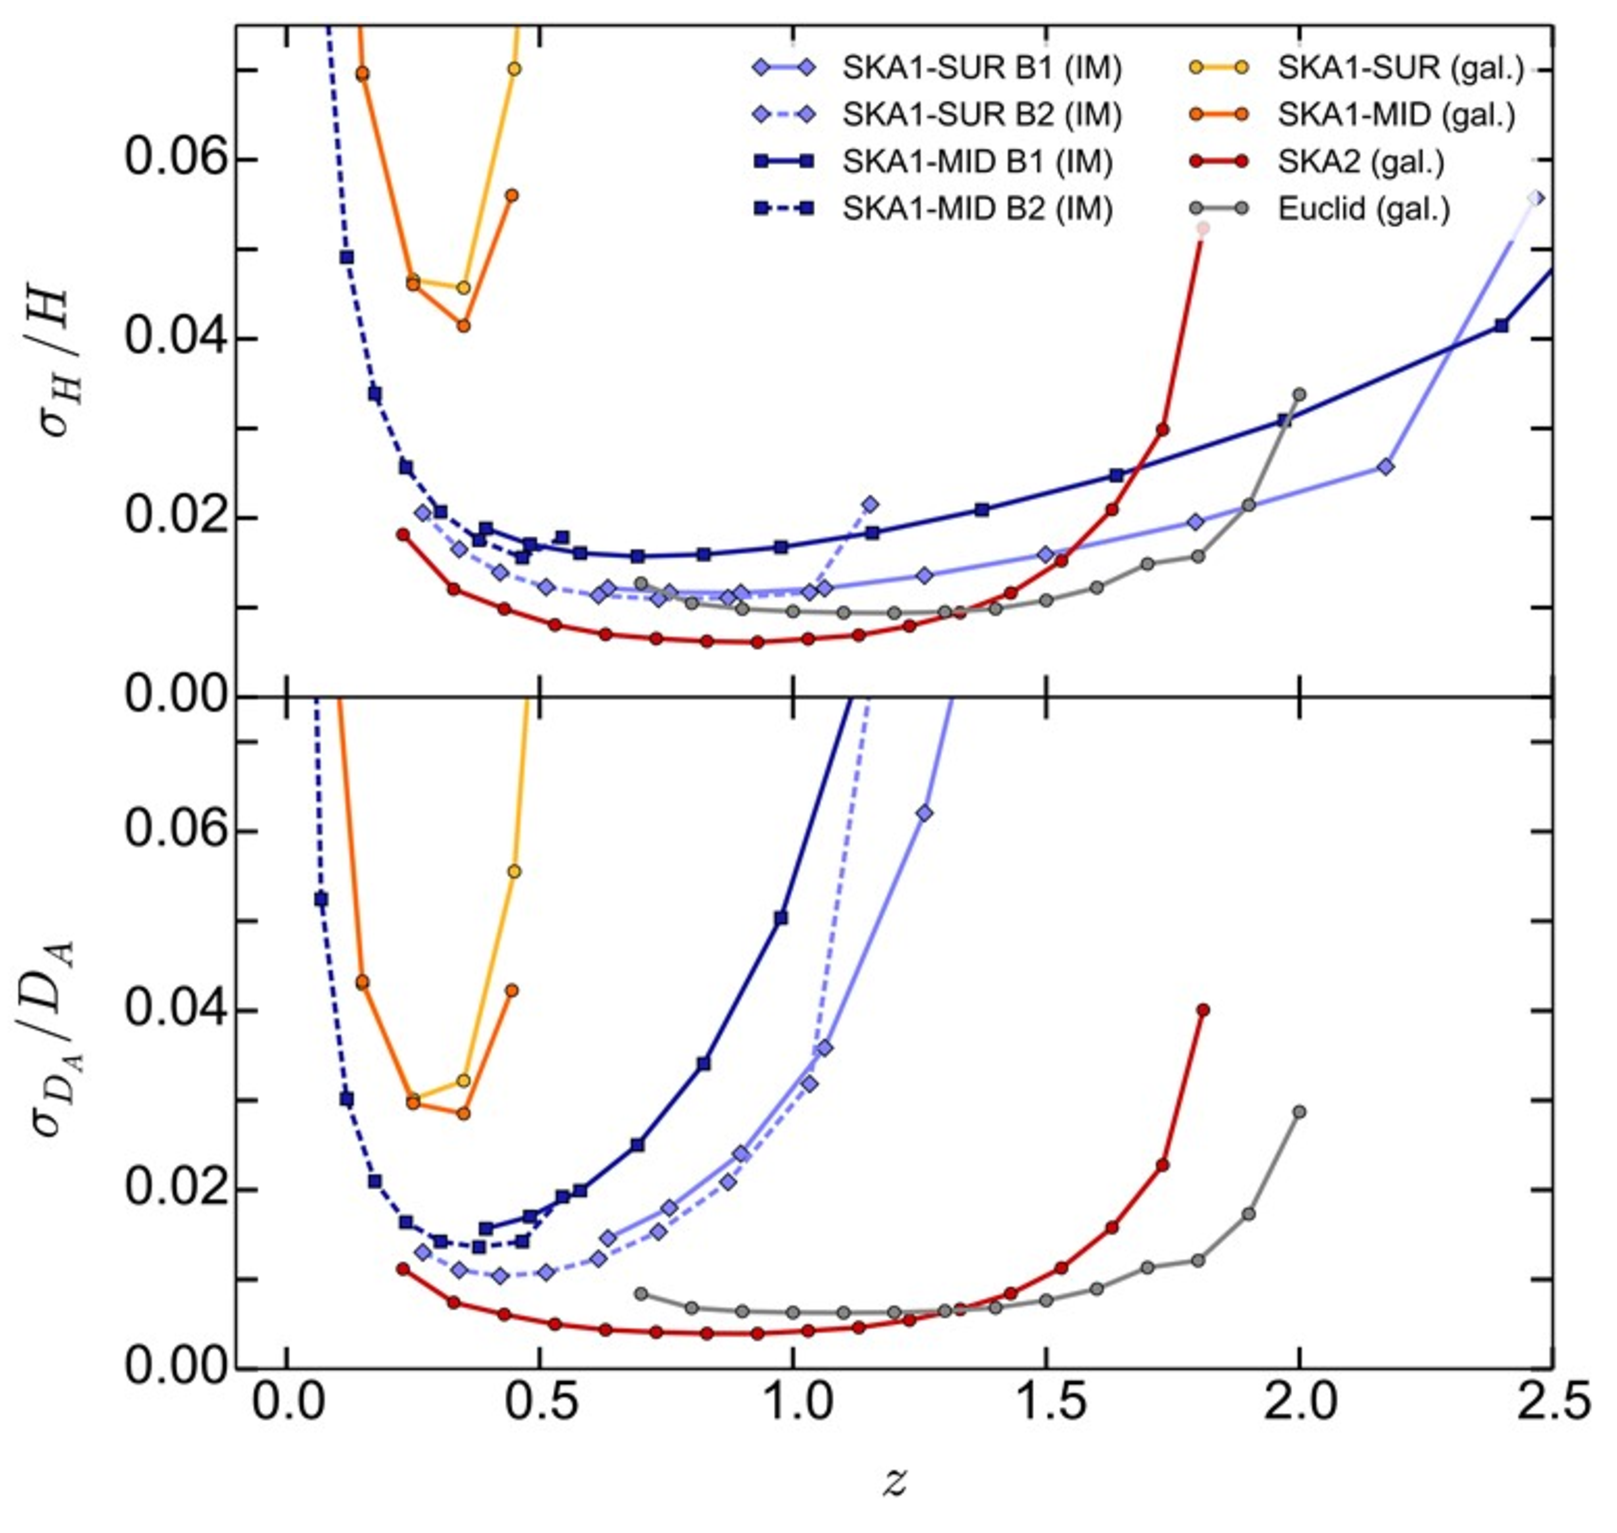
\includegraphics[width=1.0\linewidth]{cosmology/BAO_constraint.eps} 
%   \vspace{10pt}
 \end{center}
 \end{minipage}
 \begin{minipage}{0.52\hsize}
 \begin{center}
 \vspace{2.7cm}
   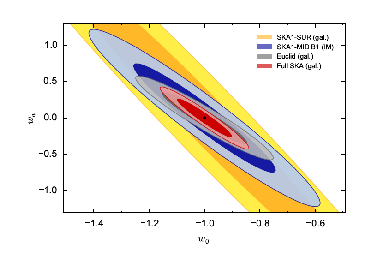
\includegraphics[width=1.0\linewidth]{cosmology/f2.eps} 
%  \vspace{-15pt}
 \end{center}
 \end{minipage}
  \caption{(左図)様々なBAO観測計画での$H$および$D_{\rm A}$の決定精度。 
(右図) 暗黒エネルギー状態方程式パラメータ$(w_0,w_a)$の決定精度。
比較のため、Euclidによる銀河サーベイ計画の感度もプロットしている。\citep{Bull:2015nra}
\label{fig:BAO fig}} 
\end{figure}
%%%%%%%%%%%%%%%%%%%%%%%%%%%%%%%%%%%%%%%%%%%%%%%%%%%%%%%%%%%%%%%%%%%%%%%%%%%%

BAOの振動スケールの測定は、主に銀河の赤方偏移探査から銀河のクラスタリング解析を行うことで行われる。\cite{2005ApJ...633..560E}によってSDSSのLRG(Luminous Red Galaxy)サンプルの二点相関関数の解析によって近傍の宇宙大規模構造において最初にBAOが検出された。実際に観測されるBAOスケールは天球面上の角度:
\begin{equation}
 d(z) = r_{\rm s}/D_{\rm V}(z),
\end{equation}
で与えられる。但し、$D_{\rm V}$は
\begin{equation}
 D_{\rm V}(z) = \left((1+z)^2D_{\rm A}^2(z)\frac{cz}{H(z)}\right)^{1/3}
\end{equation}
で与えられる。
ここで、$D_{\rm A}(z)\,, H(z)$はそれぞれ角径距離およびハッブル膨張率を表す。
これが観測されるBAOの振動スケールに一致するように宇宙論パラ
メータを決定するが、$D_{\rm V}(z)$だけを用いた宇宙論パラメータの推定には
パラメータ間の縮退が発生する。そこで、天球面方向と奥行方向のBAOの振動スケー
ルを別々に評価することで、それらの比である
\begin{equation}
 F(z) = (1+z)D_{\rm A}(z)H(z)/c
\end{equation}
を測定し、$D_{\rm V}(z)$と$F(z)$をあわせて宇宙論パラメータを推定すること
で上述の縮退を解くことができる。

BAOの振動スケールを様々な赤方偏移で測定することによって、より精密に宇宙論
パラメータを推定できる。中でもダークエネルギーのエネルギー密度とその状態
方程式パラメータ$w$の推定に利用される。現在の銀河の赤方偏移探査による
暗黒エネルギーの状態方程式パラメータの推定は、いわゆる宇宙定数と整合的
だが精度が良くない。状態方程式パラメータ(\eqref{eq:DE EOS def}, \eqref{eq:DE EOS}式)を
精密に測定することで、
暗黒エネルギーの正体の解明につながることが期待される。

\bigskip

図\ref{fig:BAO fig}左図はHI銀河赤方偏移サーベイ(gal)およびHI強度マッピングサーベイ(IM)を含む
様々なBAOの観測計画について達成可能な$H(z)$および$D_{\rm A}(z)$ の測定精度
を赤方偏移の関数として表したものである。Phase-1でのHI銀河赤方偏移サーベイでは
現在の可視光サーベイの推定精度と比較して同程度の推定精度であるのに対して、
強度マッピングサーベイでは観測するすべての赤方偏移においてHI銀河赤方偏移サーベイよりも
良い推定精度が期待される。また、Phase-2のSKAを用いたHI銀河赤方偏移サーベイではより広
い赤方偏移において1\%よりも良い推定精度で推定できると予想され、これは次世
代のEuclidなどのミッションと同程度の測定精度を達成できると期待さ
れる。これらのBAO観測計画による暗黒エネルギーの状態方程式パラメータの
推定精度が図\ref{fig:BAO fig}右図に示してある。

%%%%%%%%%%%%%%%%%%%%%%%%%%%%%%%%%%%%%%%%%%%%%%%%%%%%%%%%%%%%%%%%%%%%
\subsection{赤方偏移空間歪み}\label{cosmology.s2.ss2}
%%%%%%%%%%%%%%%%%%%%%%%%%%%%%%%%%%%%%%%%%%%%%%%%%%%%%%%%%%%%%%%%%%%%

遠方の天体までの距離は、その天体の宇宙膨張による後退速度に起因する赤方
偏移$z$と宇宙論パラメーターとに密接に関係している。その一方、その天体に
特有な特異運動(特異速度の動径成分)に起因する赤方偏移も存在する。この場
合、観測される赤方偏移の情報からだけでは本当の距離の見積もりを誤ること
になる。

この効果により、銀河の密度分布の相関を特徴付ける銀河の個数のパワースペ
クトル$P_{\rm g}^{\rm obs}(k,\mu,z)$は、真に正しい銀河のパワースペクト
ル$P_{\rm g}(k,z)$との間に、以下のようなズレが生じることが知
られている。
%%
\begin{eqnarray}
  \label{eq:Pobs}
  P_{\rm g}^{\rm obs}(k,\mu,z) = \left( 1 + \beta^2\mu^2\right) P_{\rm g}(k,z)
  \,,
\end{eqnarray}
%%
この式はカイザー公式と呼ばれ、線型近似の範囲内では妥当な近似式であ
ることが知られている。ここで、$\mu$は、着目している天体への視線方向と
波数ベクトル\mbox{\boldmath $k$}の間の方向余弦を表す。
ここで、その係数である赤方偏移空間変形パラメータ$\beta$は、後に説明する線型成長率指数$f$
および銀河密度と物質密度の間の違いを表すローカルな線型バイアスパラメータ$b$を
使って$\beta= f/b$と表される量である。
元来、真の銀河パワースペクトル$P_{\rm g}(k,z)$は、物質(ダークマタ—$+$バリオン)の
密度分布のパワースペクトル$P(k,z)$からズレていることが知られており、
先にも紹介したように、線型バイアスパラメター$b$を導入して、以下のように書き表される:
%%
\begin{eqnarray}
  \label{eq:biasedPgal}
  P_{\rm  g}(k,z)  = b^2(z) P(k,z),
\end{eqnarray}
%%
ここで、バイアスはスケールに依存しないと仮定している。
一方で、線型成長率指数$f(z)$は物質密度揺らぎの線形成長率$D(z)$を用いることで
以下のように定義される:
%%
\begin{eqnarray}
  \label{eq:growthrate}
  f(z) \equiv \frac{{\rm d} \ln D }{{\rm d} \ln a}
  \,,
\end{eqnarray}
%%
ここで$a(z)=1/(1+z)$はスケールファクターであり、$D(z)$は
今の場合次のようになる~\citep{Linder:2005in}:
%%
\begin{eqnarray}
  \label{eq:D-def}
  D(z) = a(z) \exp
    \left[
      \int_0^{a(z)}
      \left(
        \Bigl[\widetilde{\Omega}_{\rm m} (a')\Bigr]^\gamma - 1
      \right)
     \frac{d a'}{a'}
    \right]
   \,,
\end{eqnarray}
%%
但し、用いられた$ \widetilde{\Omega}_{\rm m}(a)$は、以下の定義である:
%%
\begin{eqnarray}
  \label{eq:OmegaEff}
  \widetilde{\Omega}_{\rm m}(a) = \frac{a^{-3}\Omega_{\rm m}}
{\sum_i\Omega_i 
\exp \left(
  3 \int_a^1 \left[
  w_i (a') + 1
              \right]
              \frac{d a'}{a'}
      \right)
   \,,
}
\end{eqnarray}
ここでの添字$i$は暗黒エネルギー、物質場、曲率、放射場を取り、
それぞれのエネルギー密度への寄与を表す。
このように定義した場合には、線型成長率指数$f$は
%%
\begin{eqnarray}
  \label{eq:fapprox}
  f(z) = \left[
        \widetilde{\Omega}_{\rm m}(z)
         \right]^{\gamma}
  \,,
\end{eqnarray}
のように表すことができる。
広く知られているように、一般相対論では$\gamma\simeq 0.55$である。
以下ではRSDの観測により、どのような宇宙論パラメータ
に対してどのような制限が得られるのかを簡単に紹介する。
 
\begin{description}
\item {\bf 暗黒エネルギーの状態方程式パラメータへの制限}

既に示したように、RSDを測定することで密度揺らぎの成長率$f$を観測から見積もることができる。
そのため、暗黒エネルギーと密接に関連していることからのその状態方程式パラメータ(\eqref{eq:DE EOS def}, \eqref{eq:DE EOS}式)の
推定に利用することができる。
将来のSKAによる観測により、この$2$つの
パラメータの精度よい情報が得られれば、宇宙定数とそれ以外の暗黒エネル
ギーのモデルを区別できることが期待されている。

\item {\bf 修正重力理論への制限}

\ref{cosmology.s1.ss1}節で述べてきたように、これまでに一般相対論を修正して、
暗黒エネルギーを説明しようとする試みが多数なされてきた。
%\eqref{eq:growthrate}式と
\eqref{eq:fapprox}式で導入された線型成長率指
数$f$の冪の$\gamma$は、修正重力理論に対して非常に鋭敏であることが知られている。
重力理論が一般相対性理論で記述される場合には$\gamma\approx 0.55$であるのに対し、
代表的な修正重力理論である$f(R)$重力理論では$\gamma\approx 0.40-0.43$、
DGPブレーンワールドモデルでは$\gamma\approx 0.68$程度の値をとることが示唆されてい
る~\citep{Linder:2005in}。この成長率指数を観測的に精度よく決める事により、修正
重力理論に対してする貴重な情報を得ることが出来る。
図~\ref{fig:RSD fig}左図はHI銀河赤方偏移サーベイ(gal)およびHI強度マッピングサーベイ(IM)による
RSD観測計画について、暗黒エネルギーの状態方程式パラメータ$w_0$と成長率指数$\gamma$の決定精度を
示したものである。図からわかるとおり、$\gamma$を制限することから
修正重力理論を区別するために十分な精度が期待できる。

%%%%%%%%%Figure%%%%%%%%%%%%%%%%%%%%%%%%%%%%%%%%%%%%%%%%%%%%%%%%%%%%%%%%%%%%%
\begin{figure}[t]
 \begin{minipage}{0.52\hsize}
 \begin{center}
%   \vspace{15pt}
   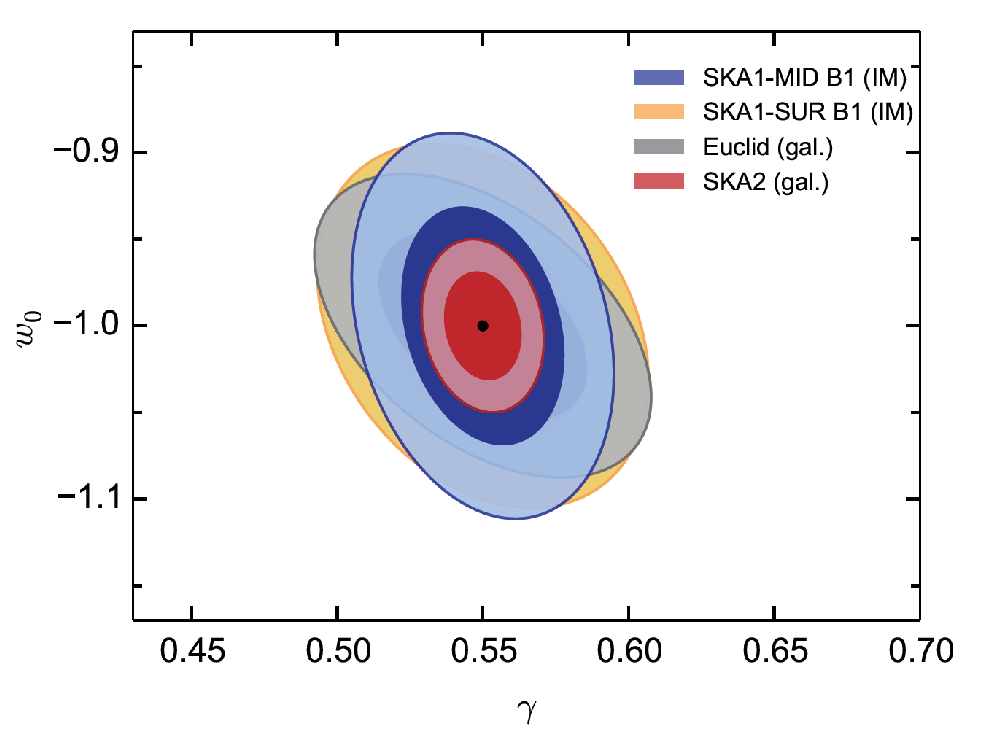
\includegraphics[width=1.0\linewidth]{cosmology/Fig3new.eps} 
%   \vspace{10pt}

 \end{center}
 \end{minipage}
 \begin{minipage}{0.52\hsize}
 \begin{center}
% \vspace{10pt}
   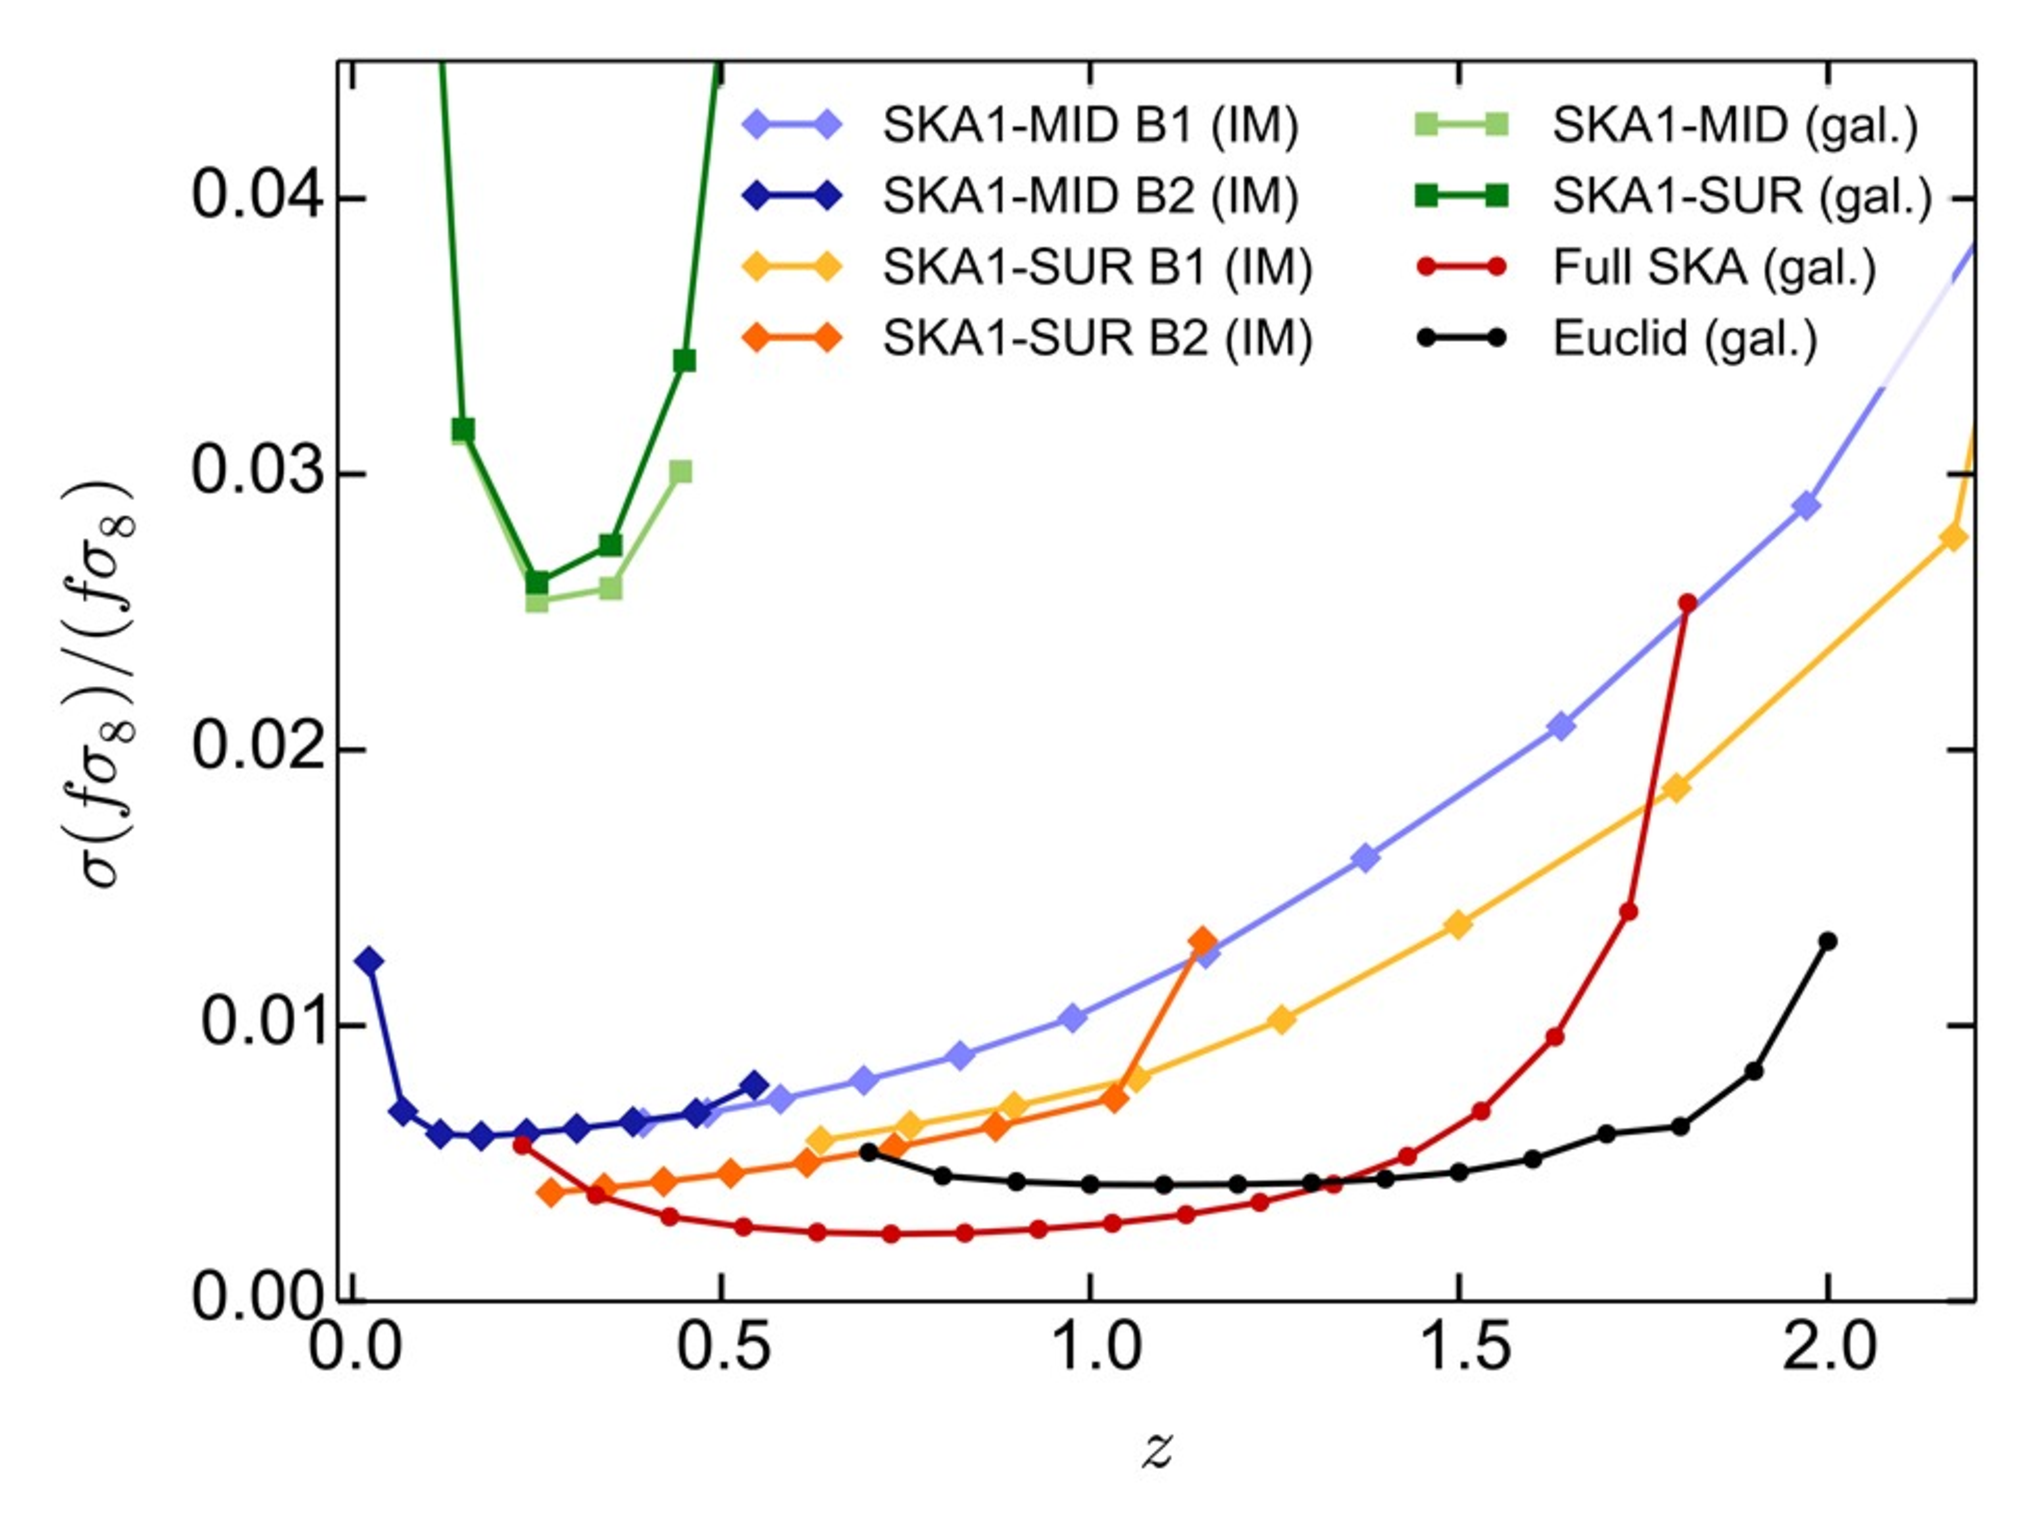
\includegraphics[width=1.0\linewidth]{cosmology/RSD_fs8.eps} 
%  \vspace{-15pt}
 \end{center}
 \end{minipage}
	\caption{(左図) 暗黒エネルギーの状態方程式パラメータ$w_0$および
	成長率指数$\gamma$の決定精度。
	(右図) $f\sigma_8$の決定精度。
	比較のため、Euclidによる銀河サーベイ計画の感度もプロットしている。\citep{Raccanelli:2015qqa}
	}
	\label{fig:RSD fig}
\end{figure}
%%%%%%%%%%%%%%%%%%%%%%%%%%%%%%%%%%%%%%%%%%%%%%%%%%%%%%%%%%%%%%%%%%%%%%%%%%%%

\eqref{eq:fapprox}式のように表せないような一般的な状況においては、質量揺らぎの分散の
平方根$\sigma_8$ (ここで$8$は半径$8h^{-1}$Mpcの球で平均した量であることを表す。)を用いて、
$f \sigma_8$および$b\sigma_8$の組み合わせについての制限を得る事により、
モデルを区別するという手法が取られる。
図~\ref{fig:RSD fig}右図に、赤方偏移$z$の関数として$f\sigma_8$の決定精度を示す。
\end{description}

%\bigskip

これまで示してきたように、RSDを観測することにより、宇宙論パラメーターを厳しく制限することができる。
特に、暗黒エネルギーのモデルパラメータへの制限はたいへん強力であり、暗黒エネルギーのモデルを
区別するために十分な感度を有している。
%ここでは、暗黒エネルギー密度が線型的に時間変化するモデルと、修正重力の単純なモデルについての解
%析結果を紹介してきた。
将来のSKAによるRSD観測により、暗黒エネルギーの正体が解明されることが期待される。


%%%%%%%%%%%%%%%%%%%%%%%%%%%%%%%%%%%%%%%%%%%%%%%%%%%%%%%%%%%%%%%%%%%%%%%%%%
\subsection{HI強度マッピング:前景放射}\label{cosmology.s2.ss3}
%%%%%%%%%%%%%%%%%%%%%%%%%%%%%%%%%%%%%%%%%%%%%%%%%%%%%%%%%%%%%%%%%%%%%%%%%%

既に述べたように、HI強度マッピングサーベイは個々の銀河を特定せず、
$1$つの大きなピクセルを用意し、そこに含まれる特定されない銀河群からの
中性水素$21$cm線を観測する。
これにより、大規模構造を$3$次元的に観測することが可能になる。
SKA-1 SURによる中性水素$21$cm観測により、$z<3$までの大規模構造を調べること
ができる。特に、宇宙論的な大規模構造の観測にはそれほどの分解能は不要であ
るので、視野の広い電波観測は都合がよい。また、$21$cm線には他の輝線と混同す
るおそれがない点も長所である。さらに干渉計による観測では、データを取得す
る際に周波数毎にビーム幅を合わせることが出来る点も、系統誤差を減らす点で
重要である。

ただし、これらは桁で大きい銀河系のシンクロトロン放射と自由-自由放射による前景放
射を除くことができればの話である。銀河系の放射は周波数方向になめらかであ
り、宇宙論的なシグナルは近似的には周波数毎に相関はないと期待されるので、
このことを用いて前景放射とシグナルを分離する手法が様々開発されている。
ここでは前景放射の差し引きの代表的な方法について紹介する~\citep{Wolz:2015sqa}。
これらの方法では、視線方向の長波長揺らぎ以外は統計誤差の範囲で再現でき
ることが分かっている。

\subsubsection{特異値分解法(SVD)}

この方法はGreen Bank Telescope (GBT)による観測で応用されている方法で、
主成分分析を経験的に発展させたものである\citep{2013MNRAS.434L..46S}。
観測機器による影響を減らすため、
データを二つのシーズンA,Bに分けて相互相関行列を考える。
これは時刻が違えばノイズ間の相関はないため、下に
述べる相互相関行列を元に前景成分を抽出する際にノイズの影響を減らすことができ
ると考えられているからである。相互相関行列は以下で与えられる。
\begin{equation}
 \bm{C}_{\rm AB} \equiv \left<
\vec{I}_{\rm A}(\theta)\left(\vec{I}_{\rm B}(\theta)\right)^{\rm T}
\right>
\end{equation}
ここで、$\vec{I}_{\rm A}(\theta)$はシーズンAでの$\theta$方向の電波強度を
あらわし、ベクトルの成分は各周波数での電波強度とする。括弧(
$\langle\cdots\rangle$ )で示した平均はピクセルでのサンプル平均とする。こ
の場合、$ \bm{C}_{\rm AB}$は実対称行列ではないので、対角化の代わりに特異
値分解$\bm{C}_{\rm AB} = \bm{U\Sigma V}^{\rm T}$を行い、$\vec{y}_{\rm
A}(\theta) = \bm{U}^{\rm T} \vec{I}_{\rm A}(\theta)$, $\vec{y}_{\rm
B}(\theta) = \bm{V}^{\rm T} \vec{I}_{\rm B}(\theta)$で定義すると、最大の
相互分散をもつ成分(これを前景放射とみなす)はシーズンAでは$y_{1}^{\rm
A}=\vec{u}_1^{\rm T} \vec{I}_{\rm A}$, シーズンBでは$y_{1}^{\rm
B}=\vec{v}_1^{\rm T} \vec{I}_{\rm B}$である。
また、これらの成分は無相関となる。今、21cmシグナルと前景放射は相関
がないと考えられていて、21cmシグナルに比べて前景放射の分散はずっと大きい
と思われているので、この成分を引くことで前景放射を除去できるというわけで
ある。
分散のもっとも大きい成分(p1
と する)は、例えばシーズンAでは$\vec{I}_{\rm p1}^{\rm A} = \vec{u}_1
\vec{u}_1^{\rm T} \vec{I}_{\rm A}$となるので、元のマップからこの成分を引
くことで前景放射の除去を行う。

\subsubsection{カルーネン$\cdot$レーベ分解}

この手法では具体的な前景放射モデルが必要である。CMBや大規模構造の研究で
使われてきており\citep{1995PhRvL..74.4369B,1996ApJ...465...34V}、最近
21cm線の研究に応用された\citep{2014ApJ...781...57S}。
相関行列がシグナル$\bm{S}$と前景放射$\bm{F}$の和で書けるとして、
$\bm{C}=\bm{S}+\bm{F} $とする。前景放射についてのみ白色化を行うと
\begin{equation}
\bm{F}^{-1/2} \bm{C} \bm{F}^{-1/2} = 
\bm{F}^{-1/2} \bm{S} \bm{F}^{-1/2} + \bm{I}
\end{equation}
を得る。この準白色化した相関行列を直交行列$\bm{O}$で対角化すると、
\begin{equation}
 \bm{F}^{-1/2} \bm{C} \bm{F}^{-1/2} = \bm{O}
(\bm{\Lambda}+\bm{I})\bm{O}^{\rm T}
\end{equation}
を得る。すなわち、直交行列の各列が$S/N$の大きい順に並んだ固有ベクトルと
なっている。この固有ベクトルを元にマップからシグナルの大きいものを抜き出せ
ばよいことになる。

\subsubsection{独立成分分析(FastICA)}

FastICAは観測されたmapを$\vec{I}(\theta)$、見積もりたいシグナルを
$\vec{s}(\theta)$としたときに、
\begin{equation}
 \vec{I} = \bm{A}\vec{s}
\end{equation}
というモデルを考え、$\bm{A}$と$\vec{s}$を同時に見積もる方法である。
そのために、各シグナル成分は独立であると仮定する。これは無相関より強い仮
定である。具体的には
\begin{equation}
 \vec{s} = \bm{W}\vec{I}
\end{equation}
という逆変換を考える際に、シグナルの各成分$s_i$の分布の非ガウス性が最大
になるように$\bm{W}$を構築すればよい。
CMBへの応用としては\cite{2002MNRAS.334...53M,2014ApJ...780...13I}、
21cm線観測への応用は\cite{2012MNRAS.423.2518C,2014MNRAS.441.3271W} がある。





%%%%%%%%%%%%%%%%%%%%%%%%%%%%%%%%%%%%%%%%%%%%%%%%%%%%%%%%%%%%%%%%%%%%%%%%%%
\subsection{HIトポロジー}\label{cosmology.s2.ss4}
%%%%%%%%%%%%%%%%%%%%%%%%%%%%%%%%%%%%%%%%%%%%%%%%%%%%%%%%%%%%%%%%%%%%%%%%%%

トポロジーは、宇宙の大規模構造を探り、
初期密度揺らぎの非ガウス性をテストするために当初導入された。
宇宙論パラメータの推定や銀河進化モデルへの制限などにも応用されている。
閾値を超える密度を持つ領域の幾何学は数学的には、ミンコフスキー汎関数を用いて
特徴付けられることが知られている~\citep{2008MNRAS.385.1613H}。
密度揺らぎ$\delta$およびその標準偏差$\sigma_0\equiv\langle\delta^2\rangle^{1/2}$を
用いることで、与えられた閾値$\nu =\delta /\sigma_0$を超えた等密度面の
ミンコフスキー汎関数は以下の$4$つ定義できる:
体積$V_0(\nu )$、表面積$V_1(\nu )$、平均密度$V_2(\nu )$、オイラー数$V_3(\nu)$である。
この中でも、オイラー数$V_3(\nu )$はジーナス(Genus)と呼ばれる量$G(\nu)$と
$V_3(\nu )=2-2G(\nu )$と関連している。
ジーナスは、考えている領域に存在する穴の数から孤立した領域の数を引いた量として定義される。
密度揺らぎが厳密にガウス分布に従う場合には、全てのミンコフスキー汎関数は
解析的に解かれており、
特に単位体積あたりのジーナス$G(\nu )$は次のように表す事が出来ることが知られている:
\begin{equation}
G(\nu)={\cal A}\left( 1-\nu^{2}\right) e^{-\nu^{2}/2},
\label{eq:genus}
\end{equation}
ここで、${\cal A}$は密度揺らぎ$\delta$のパワースペクトルを用いて得られる振幅である。
密度揺らぎのガウス分布からのどのようなズレも非ガウス性の証拠となりえるとともに、原始非ガウス性を
制限する手法となる。
原始非ガウス性はあらゆる高次モーメントによっても引き起こされることから、この研究は
これまでよく行われてきた$3$点相関関数つまりはバイスペクトルによる手法と相補的であると言える。
21cm線マップから得られるミンコフスキー汎関数は、低赤方偏移の大規模構造だけでなく、
高赤方偏移の再電離期における中性水素の分布の分布をも特徴付けることができる。
宇宙論の文脈の中で場の幾何学的性質を探るのが有効な手段となる分野は、以下の様なものが挙げられる。

\begin{description}
\item {\bf 原始非ガウス性 }

\ref{cosmology.s1.ss1}節で既に述べたように、原始非ガウス性は初期宇宙に対して深い理解を与えることができる。
初期密度揺らぎが\eqref{eq:fNL def}式で与えられる場合、
ジーナスは厳密なガウス分布の場合の\eqref{eq:genus}式からずれる。
ジーナスのガウス分布からのズレは、$2$次まで展開することで次のように得ることができる:
\begin{equation}
\Delta(\nu)\equiv \delta\left (\frac{G}{\cal A}\right) =-e^{-\nu^{2}/2}\biggl[\left( S_{\rm pri}^{(1)}-S_{\rm pri}^{(0)}\right) H_{3}(\nu )+\left( S_{\rm pri}^{(2)}-S_{\rm pri}^{(0)}\right) H_{1}(\nu ))\biggr]\sigma_{0},
\end{equation}
ここで、$H_n$はエルミート多項式であり、$S_{\rm pri}^{(a)}$は歪度パラメータと呼ばれる量である~\citep{2006ApJ...653...11H}。
$S^{(0)}_{\rm pri}$は揺らぎの歪度を表しているのに対し、$S^{(1)}_{\rm pri}$および$S^{(2)}_{\rm pri}$はその微分と関連する量であることから
\eqref{eq:fNL def}式に現れる非線形パラメータ$f_{\rm NL}$に依存している。
よって、これを測定することに事により、$f_{{\rm NL}}$への制限を得る事が出来る。
SKAでは$\sigma(f_{\rm NL})=20$程度の制限が予想される(図\ref{fig:fnl})。
原始非ガウス性が\eqref{eq:fNL def}式で書けない場合であってもジーナスに影響が及ぶことから
HIトポロジーは一般的な原始非ガウス性を制限しうる。

\item {\bf 暗黒エネルギーと修正重力理論 }

大規模構造のトポロジーは構造の成長と関係付けることができる。
実際、線形成長のみを考えるときには\eqref{eq:genus}式の${\cal A}$は保存し、
スムージングスケールを$R_{\cal G}$としたとき、
${\cal A}_{\rm Y}(z,R_{{\cal G},{\rm Y}})R_{\rm Y}^{3}={\cal A}_{\rm X}(R_{{\cal G},{\rm X}})R_{{\cal G},{\rm X}}^{3}$
なる関係が成り立つことが期待される~\citep{Park:2009ja}。
ここで、Xは真の宇宙論パラメータを表すのに対し、Yは採用した宇宙論パラメータを表し、一般に両者は異なっていてよい。
異なる宇宙論模型のスムージングスケール$R_{\cal G}$は、$(R_{{\cal G},{\rm X}}/R_{{\cal G},{\rm Y}})^{3}=(D_{\rm A}^{2}/H)_{\rm X}/(D_{\rm A}^{2}/H)_{\rm Y}$
を通じて結びつけられている。
%ここで、$D_{\rm A}$および$H$は角径距離およびハッブル膨張率を表す。
この効果を用いることで、大規模構造のトポロジーは標準ものさしとして用いる事ができ、暗黒エネルギーモデルへの制限を与える事が出来る。
また、修正重力理論を考える場合、揺らぎの成長率が一般相対論の場合と異なり、スケール依存性を持つことが知られている。
%その結果、ジーナスカーブに変更が加えられることになる。
暗黒エネルギーモデルへの制限と同様の理由で、修正重力理論のモデルへの制限も行う事が出来る。


\item {\bf 再電離 }

トポロジー解析は宇宙再電離の詳細な過程に対して直接的で鋭敏なプローブを与える。
トポロジーの定量的な観測量としてHIの密度等高線のジーナスを用いることで、
銀河間物質の再電離過程は次の4つのフェーズに分離することができる:
(i)再電離前、(ii)再電離開始後HII領域の重なり合いが始まる前、 (iii)重複期、 (iv)重複後、である。
(i)のフェーズでは、HIの分布は原始密度揺らぎを反映している。
そのため、ジーナスカーブはガウス分布と整合的であり、トポロジーはHI密度の
線形発展に対して変わらない。
(ii)は孤立したHIIバブルによるトポロジーによって特徴付けられる。
このフェーズの初期では、HIIバブルが徐々に増えて行くため、ジーナスカーブ
の振幅も徐々に増えて行く。
しかし、バブルの重なり合いが起きる(iii)ではジーナスカーブの振幅は徐々に減少していく。
(iv)では銀河間物質はほとんどイオン化しており、ジーナスカーブの成長は孤立した中性水素領域の数の
減少と整合的になる。
このように、ジーナスは中性水素領域のトポロジーの時間発展を追う事ができ、
さらに、再電離の異なる段階の赤方偏移を決定できるため、再電離シナリオの区別に
応用する事が出来ると考えられる~\citep{2014JKAS...47...49H}。
\end{description}


%%%%%%%%%%%%%%%%%%%%%%%%%%%%%%%%%%%%%%%%%%%%%%%%%%%%%%%%%%%%%%%%%%%%%%%%%%
\subsection{超地平線スケール宇宙論}\label{cosmology.s2.ss5}
%%%%%%%%%%%%%%%%%%%%%%%%%%%%%%%%%%%%%%%%%%%%%%%%%%%%%%%%%%%%%%%%%%%%%%%%%%

非常に大きなスケールに隠されている宇宙論的な情報は非常に重要になりえる。
大スケールでは構造の非線形発展を安全に無視することができるため、
揺らぎの発展は線形領域に留まっている。
また、物理過程はほとんど重力的な相互作用によって記述され、宇宙物理的な複雑な
プロセスを考慮に入れる必要がない。
そのような意味で、大スケールを観測することで非常にクリーンな探査が可能である。

大スケールは精密な理論予測が容易であるが、大スケールを観測することは非常に難しい。
大スケールに対応するような非常に小さなフーリエモードを探査するためには、
大角度を観測するだけでは不十分であることに注意する。
天球面上でどれだけ大スケールを観測しても、$3$次元の意味で観測しうるスケールは
視線方向成分で制限されてしまう。つまり、十分深いサーベイが必要がある。
二つ目の問題としては宇宙の単一性による有限サンプルから現れるノイズ:コズミックバリアンス(Cosmic Variance; CV)である。
どれだけ大きな体積を持ってきても観測体積内に含まれる天体が少数であれば、
その数で制限されてしまう。
SKAはこの状況を打破しうる観測であり、大スケールに関する研究を大いに推し進めることができる~\citep{Camera:2015yqa}。


%%%%%%%%%Figure%%%%%%%%%%%%%%%%%%%%%%%%%%%%%%%%%%%%%%%%%%%%%%%%%%%%%%%%%%%%%
\begin{figure}[t]
 \begin{minipage}{0.53\hsize}
 \begin{center}
%   \vspace{10pt}
   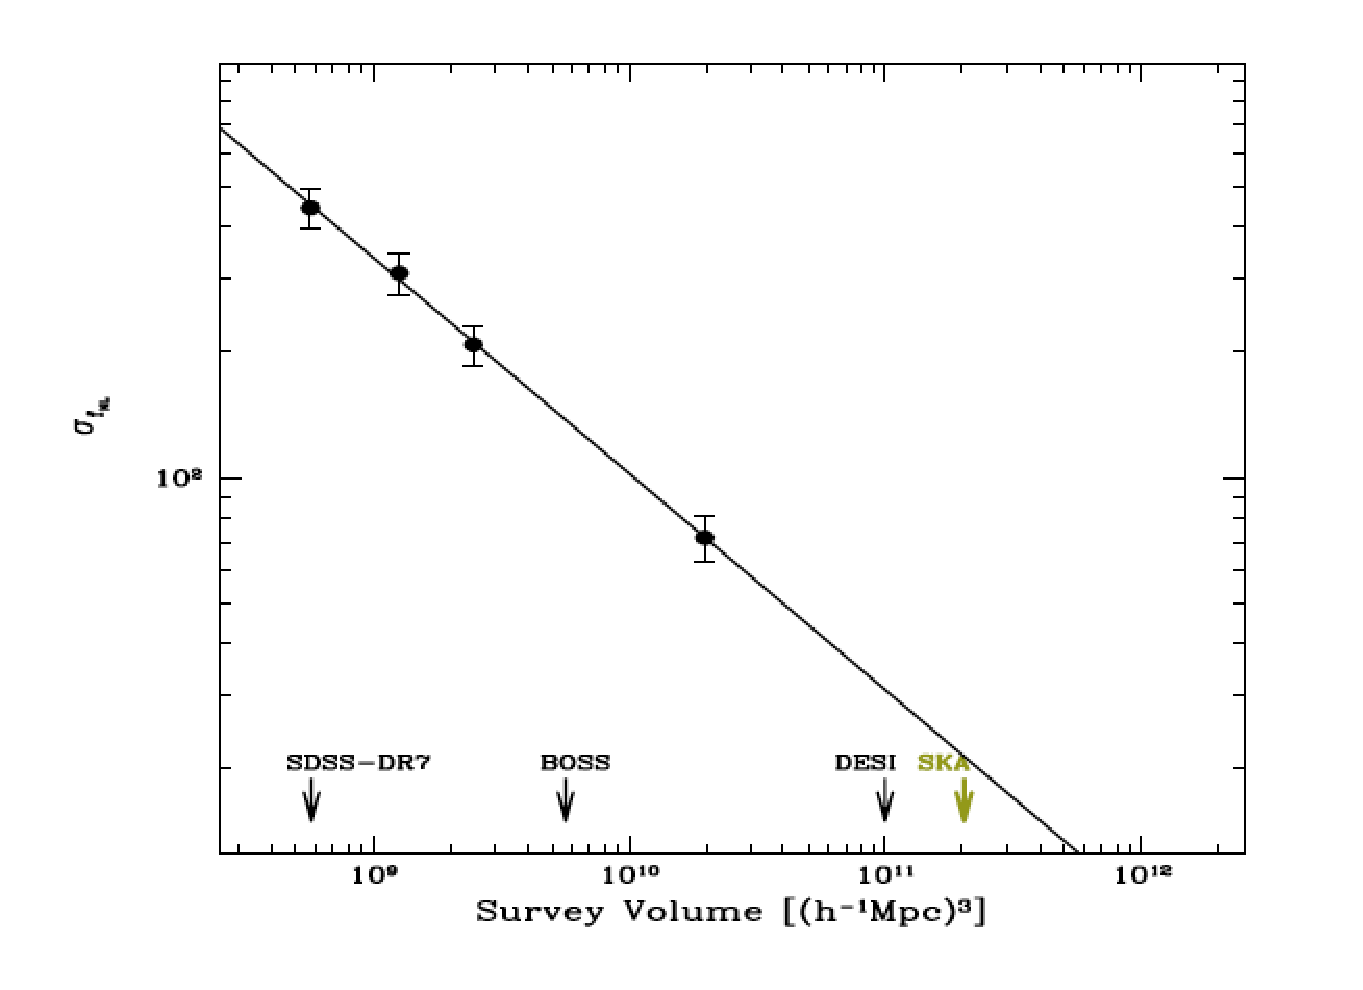
\includegraphics[width=1.0\linewidth]{cosmology/fnl.eps} 
%   \vspace{10pt}
   \caption{ジーナス統計を用いた$f_{\rm NL}$の決定精度。%SKAでは$2\times 10^{11}(h^{-1}{\rm Mpc})^{3}$のサーベイ体積を仮定。
}
\label{fig:fnl}
 \end{center}
 \end{minipage}
 \begin{minipage}{0.51\hsize}
 \begin{center}
   \vspace{5pt}
   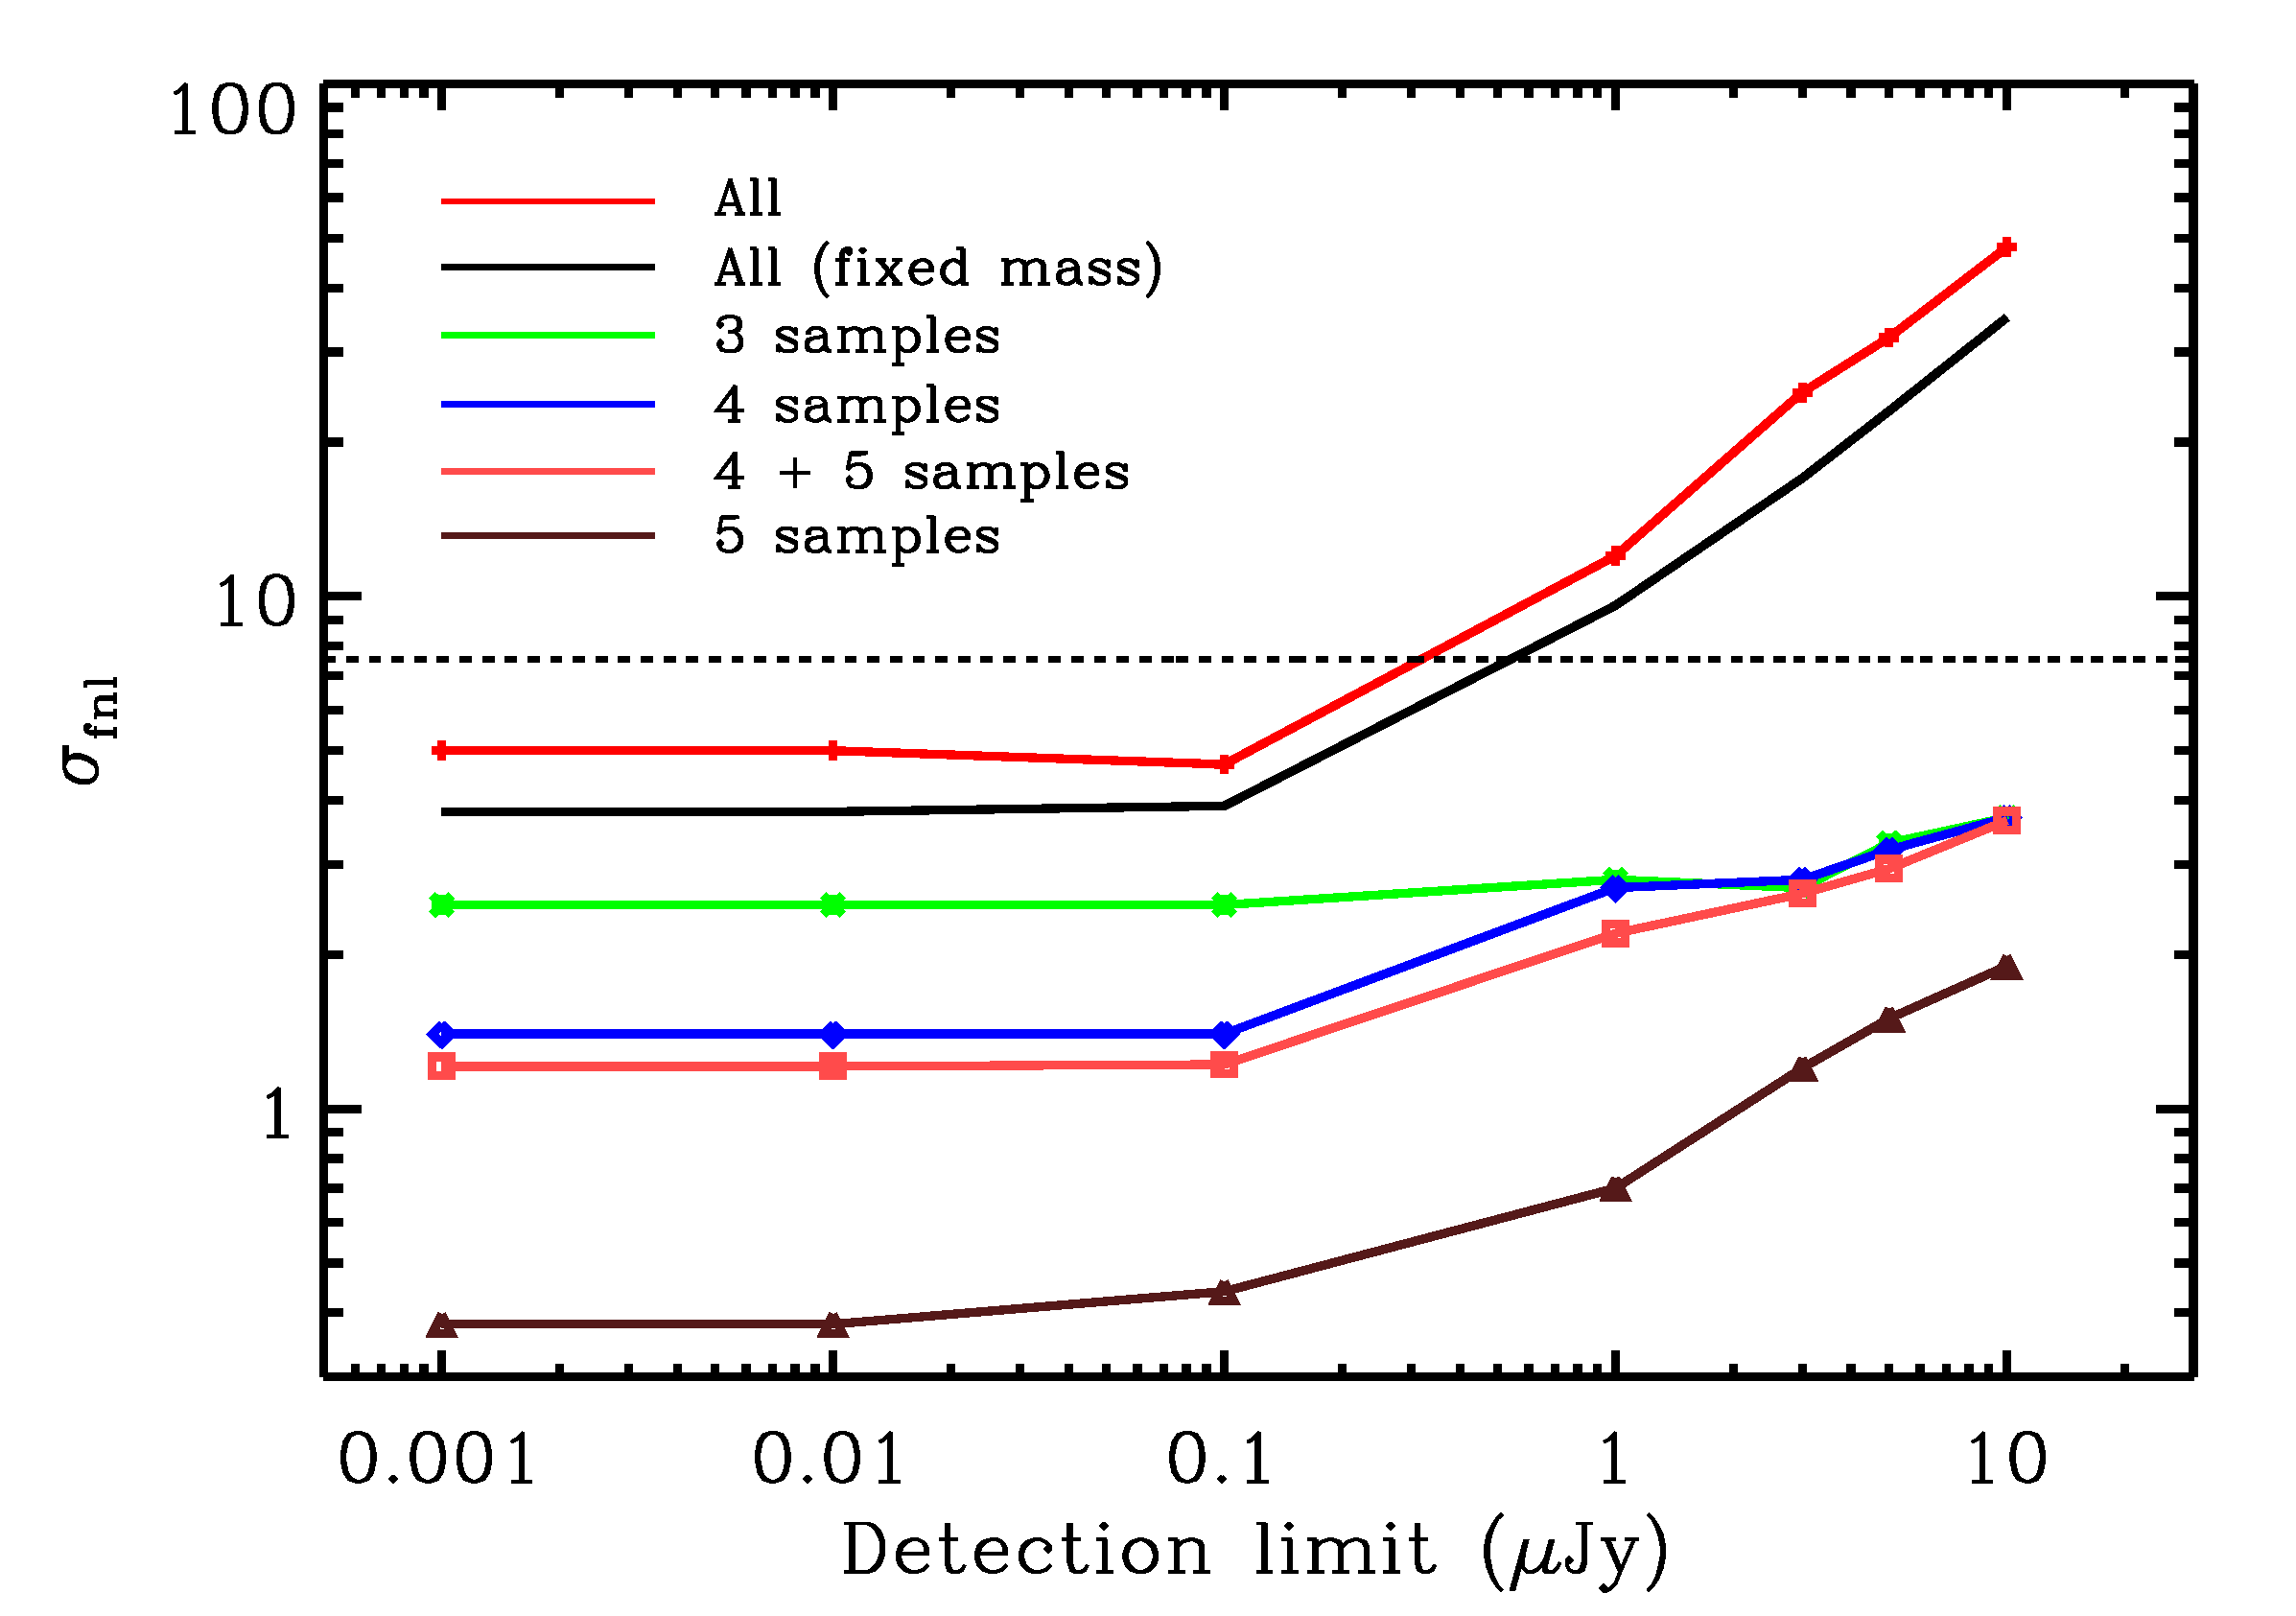
\includegraphics[width=1.0\linewidth]{cosmology/fig5.eps} 
%  \vspace{-15pt}
  \caption{マルチトレーサー法を用いた場合の$f_{\rm NL}$の決定精度~\citep{Ferramacho:2014pua}。
}
\label{fig:Ferramacho}
 \end{center}
 \end{minipage}
\end{figure}
%%%%%%%%%%%%%%%%%%%%%%%%%%%%%%%%%%%%%%%%%%%%%%%%%%%%%%%%%%%%%%%%%%%%%%%%%%%%


%%%%%%%%%%%%%%%%%%%%%%%%%%%%%%%%%%%%%%%%%%%%%%%%%%%%%%%%%%%%%%%%%%%%%%%%%
%=======================================================================%
\subsubsection{宇宙論的な大スケールを探査する重要性}
%=======================================================================%
%%%%%%%%%%%%%%%%%%%%%%%%%%%%%%%%%%%%%%%%%%%%%%%%%%%%%%%%%%%%%%%%%%%%%%%%%

%これまでにない規模の大体積を探査することにより、
%「インフレーションを起こしたメカニズムは何か?」
%「大スケールにおいて一般相対論は実現しているのか?」
%というような宇宙論における基礎的な疑問に答えていくことができる。
%
\ref{cosmology.s1.ss1}節で述べたように、原始非ガウス性はインフレーション模型を決定付けるために有用である。
現在最も厳しい原始非ガウス性の制限はPlanck衛星によるものであるが、将来のCMB観測を用いたとしても
Planck衛星の結果以上に改善することは難しい。
原始非ガウス性を制限する新しいフロンティアは物質分布の大体積のサーベイである。
%
同様に、宇宙論的スケールにおける一般相対論のテストも大規模構造の観測によって行うことができる。
加えて、より大スケールを観測し、統計を稼ぐことにより、暗黒エネルギーや修正重力理論の
厳しい制限を与えることができる。
以下、SKAサーベイで期待される成果についてより具体的に述べる。

\begin{description}
\item {\bf 一般相対論効果 }

一般相対論的効果は、過去の光円錐上において数密度や輝度温度揺らぎを観測する際に現れる。
これまでの解析では、ニュートン近似への標準的な補正として赤方偏移歪みと重力レンズによる増幅効果
のみを部分的に取り入れてきた。
しかし、これらの効果は十分小スケールでのみ重要になってくる。
将来の広範かつ深いサーベイにおいては、宇宙物理学的な複雑なプロセスは無視できても
全ての一般相対論的補正を含むような精緻な模型を用いることが
重要になる~\citep{Yoo:2010ni,Bonvin:2011bg,Challinor:2011bk,Bruni:2011ta}。
%その特徴の一つとして、一般相対論効果を含む2点相関関数をルジャンドル陪関数で展開したときには、
%標準的な解析ではゼロであったパリティ奇のモードが寄与することが指摘されている。

\item {\bf 原始非ガウス性 }

大スケールを探査することで宇宙原始揺らぎの重要な情報を得ることができる。
これまで原始揺らぎの非ガウス性を探る最もよいプローブはCMB温度揺らぎのバイスペクトルであった。
しかし、原始非ガウス性は、背後にある物質分布のバイアスに対してスケールおよび赤方偏移依存性を付与する
ことが明らかとなった\citep{Dalal:2007cu,Matarrese:2008nc,Schmidt:2010gw,Desjacques:2008vf}。
原始非ガウス性がないときの大スケールのバイアスを$b$と書いたとき、
\eqref{eq:fNL def}式で与えられる原始非ガウス性による補正項は次のように書ける:
\begin{align}
	\Delta b(z,k)=3[b(z)-1]\frac{\Omega_{\rm m}H_0^2\delta_c}{k^2T(k)D(z)}f_{\rm NL}
	\,.\label{eq:scale dependent bias}
\end{align}
ここで、$\delta_c$は崩壊時の物質揺らぎの臨界値、$T(k)$は遷移関数、$D(z)$は密度揺らぎの線形発展因子である。
原始非ガウス性の効果により、パワースペクトルは大スケールで$k^{-2}$として振舞う。
これは一般相対論的効果が効くスケールと一致しており、原始非ガウス性の精密な予言のために一般相対論的効果を
適切に取り入れることが必要である。


\item {\bf 修正重力理論 }

一般相対論は実験室や太陽系スケールでは精緻にテストされてきたが、宇宙論スケールではいまだ弱い制限しかない。
暗黒エネルギーの文脈において大スケールにおける一般相対論のテストは非常に注目されている。
\ref{cosmology.s1.ss1}節で述べたように、暗黒エネルギーの代替要素としての修正重力理論はこれまで非常に多く提案されて
おり、これらの多くは暗黒エネルギーの状態方程式(\eqref{eq:DE EOS def}式)を変更することから、
これを精密に探査することで模型を区別することができると期待されている。
修正重力理論の暗黒エネルギー以外の典型的な予言としては揺らぎの発展史への修正が挙げられる。
その中でも揺らぎの成長率は最も揺らぎの発展史に鋭敏であり、HI銀河赤方偏移サーベイや
HI強度マッピングサーベイによりRSD (\ref{cosmology.s2.ss2}節)を用いることで測定することができると期待されている。

\end{description}


%%%%%%%%%%%%%%%%%%%%%%%%%%%%%%%%%%%%%%%%%%%%%%%%%%%%%%%%%%%%%%%%%%%%%%%%%
%=======================================================================%
\subsubsection{宇宙論的な大スケールの観測手法}
%=======================================================================%
%%%%%%%%%%%%%%%%%%%%%%%%%%%%%%%%%%%%%%%%%%%%%%%%%%%%%%%%%%%%%%%%%%%%%%%%%

%%%%%%%%%%%%%%%%%%%%%%%%%%%%%%%%%%%%%%%%%%%%%%%%%%%%%%%%%%%%%%%%%%%%%%%%%
%=======================================================================%
\paragraph{再イオン化期後の強度マッピング}
%=======================================================================%
%%%%%%%%%%%%%%%%%%%%%%%%%%%%%%%%%%%%%%%%%%%%%%%%%%%%%%%%%%%%%%%%%%%%%%%%%

$21$cmパワースペクトルをモデル化する際、物質場とHIパワースペクトルの間の関係を決める
バイアス関数の定量化は難しい。
バイアスを理解するために、大規模構造の流体計算や$N$体計算の結果から擬似HIパワースペクトル
を抜き出す様々な手法が開発されている。
その中で、$k\lesssim 1\,h{\rm Mpc}^{-1}$のスケールではバイアスは定数に漸近
することが示されている~\citep{Villaescusa-Navarro:2014cma}。
バイアスの完全な特徴を掴むまでには至っていないが、十分大スケールでHIバイアスを定数だと
仮定することで、修正重力理論や原始非ガウス性の研究に応用することができる。

\begin{description}
\item {\bf スケールに依存するバイアスによる原始非ガウス性の探査 }

HIバイアスを通じて、原始非ガウス性を制限することができる~\citep{Camera:2013kpa}。
再イオン化後では、ほとんどの中性水素は銀河内にしか存在しないと考えられることから、
中性水素のパワースペクトルは銀河に付随する暗黒物質ハロー分布にバイアスされていると考えられる。
実際、視線方向の散乱および自己吸収を無視した場合、HI線放射はハローの微分数密度と関連付けることができ、
これによりバイアスを推定することができる。
SKA1-MIDを用いた場合の原始非ガウス性の決定精度は
$\sigma (f_{\rm NL})\sim 2$となる。
SKA2では$\sigma (f_{\rm NL})\lesssim 1$を達成できる。

\item {\bf バイスペクトルによる原始非ガウス性の探査 }
銀河に比べ、HIの物質分布へのバイアスは相対的に小さい。
そのため、線形バイアスおよび非線形バイアスの寄与を加えた樹形バイスペクトル
をHIのバイスペクトルとしてモデル化することができる。
高赤方偏移において原始密度揺らぎの寄与はより重要になる。
SKA 1-MIDでは$\sigma (f_{\rm NL})=45.7$であり、
SKA2においては$\sigma (f_{\rm NL})=6.6$まで改善する。
\end{description}


%%%%%%%%%%%%%%%%%%%%%%%%%%%%%%%%%%%%%%%%%%%%%%%%%%%%%%%%%%%%%%%%%%%%%%%%%
%=======================================================================%
\paragraph{再イオン化期における強度マッピング}
%=======================================================================%
%%%%%%%%%%%%%%%%%%%%%%%%%%%%%%%%%%%%%%%%%%%%%%%%%%%%%%%%%%%%%%%%%%%%%%%%%

原始非ガウス性は初期星形成銀河ハローのクラスター化にも影響を及ぼす。
再イオン化時に星形成銀河ハローは銀河間物質中にイオン化されたパッチの
ネットワークを形成することから、イオン化水素の分布には原始非ガウス性の
痕跡が残っていると期待される。
ここで、イオン化密度バイアスは再イオン化模型から導くことができる。
SKA1-LOWでは、この手法による原始非ガウス性への制限は$\sigma (f_{\rm NL})=7.4$となる。
full SKAを用いることができるならば制限は$\sigma (f_{\rm NL})=4.7$まで改善することができる~\citep{Mao:2013yaa}。


%%%%%%%%%%%%%%%%%%%%%%%%%%%%%%%%%%%%%%%%%%%%%%%%%%%%%%%%%%%%%%%%%%%%%%%%%
%=======================================================================%
\paragraph{マルチトレーサー法}
%=======================================================================%
%%%%%%%%%%%%%%%%%%%%%%%%%%%%%%%%%%%%%%%%%%%%%%%%%%%%%%%%%%%%%%%%%%%%%%%%%

大スケールでの統計解析はスケールに依存するバイアスを通じて非ガウス性を探査することに対して非常に有利だが、精度は本質的にCVによって制限される。\cite{Seljak:2008xr}によって異なるバイアスを持つ2つ以上の観測量を用いることでCVをうまく回避する方法が提案されている。これをマルチトレーサー法と呼ぶ。
この方法の基本的なアイデアとしては、少なくとも2つの異なるバイアスを持つ観測量を用意することでバイアスの比の決定精度についてはショットノイズだけによって決まるようにできることにある。\cite{Ferramacho:2014pua}においてこれをSKAの連続波サーベイに適用している。SKA1においてマルチトレーサー法を用いないと$\sigma (f_{\rm NL})=32$であるのに対し、用いることで
$\sigma (f_{\rm NL})\sim 2.9$まで改善する。
SKA2においては$\sigma (f_{\rm NL})\sim 0.7$にまで到達することができると期待されている。
図\ref{fig:Ferramacho}にフラックスカットの関数として$f_{\rm NL}$の決定精度を図示する。

\bigskip

ここまで示したように、SKAによって可能になる大スケールの観測によって、
「インフレーションを起こしたメカニズムは何か」、「大スケールにおいて一般相対論は実現しているか」
というような宇宙論における基礎的な疑問に答えることができるようになる。
特に、これまで最も厳しい制限を与えてきたCMBによる制限を凌ぐ制限を与えることが可能になる。
SKAが与えうる制限はEuclid衛星に代表される他波長の観測計画(\ref{cosmology.s1.ss2}節)と競合しているが、
これらのノイズの統計的性質はそれぞれに異なっていることから、それぞれの制限は相補的である。



%%%%%%%%%%%%%%%%%%%%%%%%%%%%%%%%%%%%%%%%%%%%%%%%%%%%%%%%%%%%%%%%%%%%%%%%%%
\subsection{弱重力レンズ}\label{cosmology.s2.ss6}
%%%%%%%%%%%%%%%%%%%%%%%%%%%%%%%%%%%%%%%%%%%%%%%%%%%%%%%%%%%%%%%%%%%%%%%%%%

%%%%%%%intro%%%%%%%%%%%%%%%%%%%%%%%%%%%%%%%%%%%%%%%%%%%%%%%%%%%%%%%%%%%%%%%%
SKAでは銀河探査を利用した弱重力レンズ探査に加え、
中性水素ガス21cm線の強度分布の観測を利用した手法も考えられており、
特に後者は銀河探査よりも大きな赤方偏移の時代の観測に利用できると期待されている。
本節では,これらSKAを利用した弱重力レンズ探査について以下で解説を行っていく。

%%%%%%%%%%%%%%%%%%%%%%%%%%%%%%%%%%%%%%%%%%%%%%%%%%%%%%%%%%%%%%%%%%%%%%%%%%%%
\subsubsection{銀河の弱重力レンズ効果の測定}
%
銀河に対する弱重力レンズ効果は、観測された銀河の形が歪む効果として観測される。
現在この銀河探査による弱重力レンズ効果の観測は、可視光による観測が先行しており、
CFHTLenS surveyなどで実際にその効果が精度良く観測されている~\citep{Heymans:2013fya}。
%
しかしSKAの様な電波領域における高視野,高解像度の観測が実現すれば、
従来可視光の領域であった弱重力レンズ探査を
電波観測によって行うことができるようになると期待されており、
現在その観測における問題点や解析手法に対する研究が精力的に行われている~\citep{Brown:2015vqa,Patel:2015cra}。

弱重力レンズ効果の観測においては、銀河の形状を解析する必要なら観測機器の角分解能に依存する。
SKAは他波長、特に光赤外観測計画(\ref{cosmology.s1.ss2}節)に比べ、角分解能は若干見劣りする。
しかし、SKAはほぼ全体にわたる広い立体角($\sim 3\pi$ steradian)を観測するとともに、
$z\gtrsim 2$のような大きな赤方偏移を持つ銀河を観測しうることから、他波長の観測と
競合するほどの性能を持つ。
%
例えば図\ref{fig:WL_fig1}の左図は、
SKAによって連続波を用いて銀河探査を行った場合に期待される弱重力レンズ効果によって生じる歪みの効果
(歪み場相関関数のパワースペクトル)とその測定エラーである。
光赤外による銀河探査計画であるEuclidと比較して、より大きな赤方偏移の銀河を多数観測することが
可能であり、その結果SKAを利用することで非常に精度よく歪み場の観測が可能であることがわかる。
%
また図\ref{fig:WL_fig1}の右図は
SKA2の弱重力レンズ効果の観測を行った場合に期待される、
物質(暗黒物質とバリオン)の密度パラメータ$\Omega_{\rm m}$、
及び質量揺らぎの分散の平方根$\sigma_{8}$に対する制限の図である。
%
特に質量揺らぎの分散$\sigma_{8}$は、密度揺らぎの成長を通して
暗黒エネルギーの性質に依存するため、
$\sigma_{8}$の精密な測定は正体不明の暗黒エネルギーの性質を調べる上で
きわめて重要であると言える。
%
%なおこの
解析結果によれば、SKA1-earlyでさえ、
現在の可視光による弱重力レンズ効果の観測と比較して
数倍程度強い制限を与えることができると期待できる。
またSKA1は光赤外将来計画DESと並び、
さらにSKA2のおいてはEuclidと比肩するほどの
観測性能を持つ。
SKAによる弱重力レンズ効果の観測が非常に強力であることが分かる。


%%%%%%%%%Figure%%%%%%%%%%%%%%%%%%%%%%%%%%%%%%%%%%%%%%%%%%%%%%%%%%%%%%%%%%%%%
\begin{figure}[t]
 \begin{minipage}{0.53\hsize}
 \begin{center}
   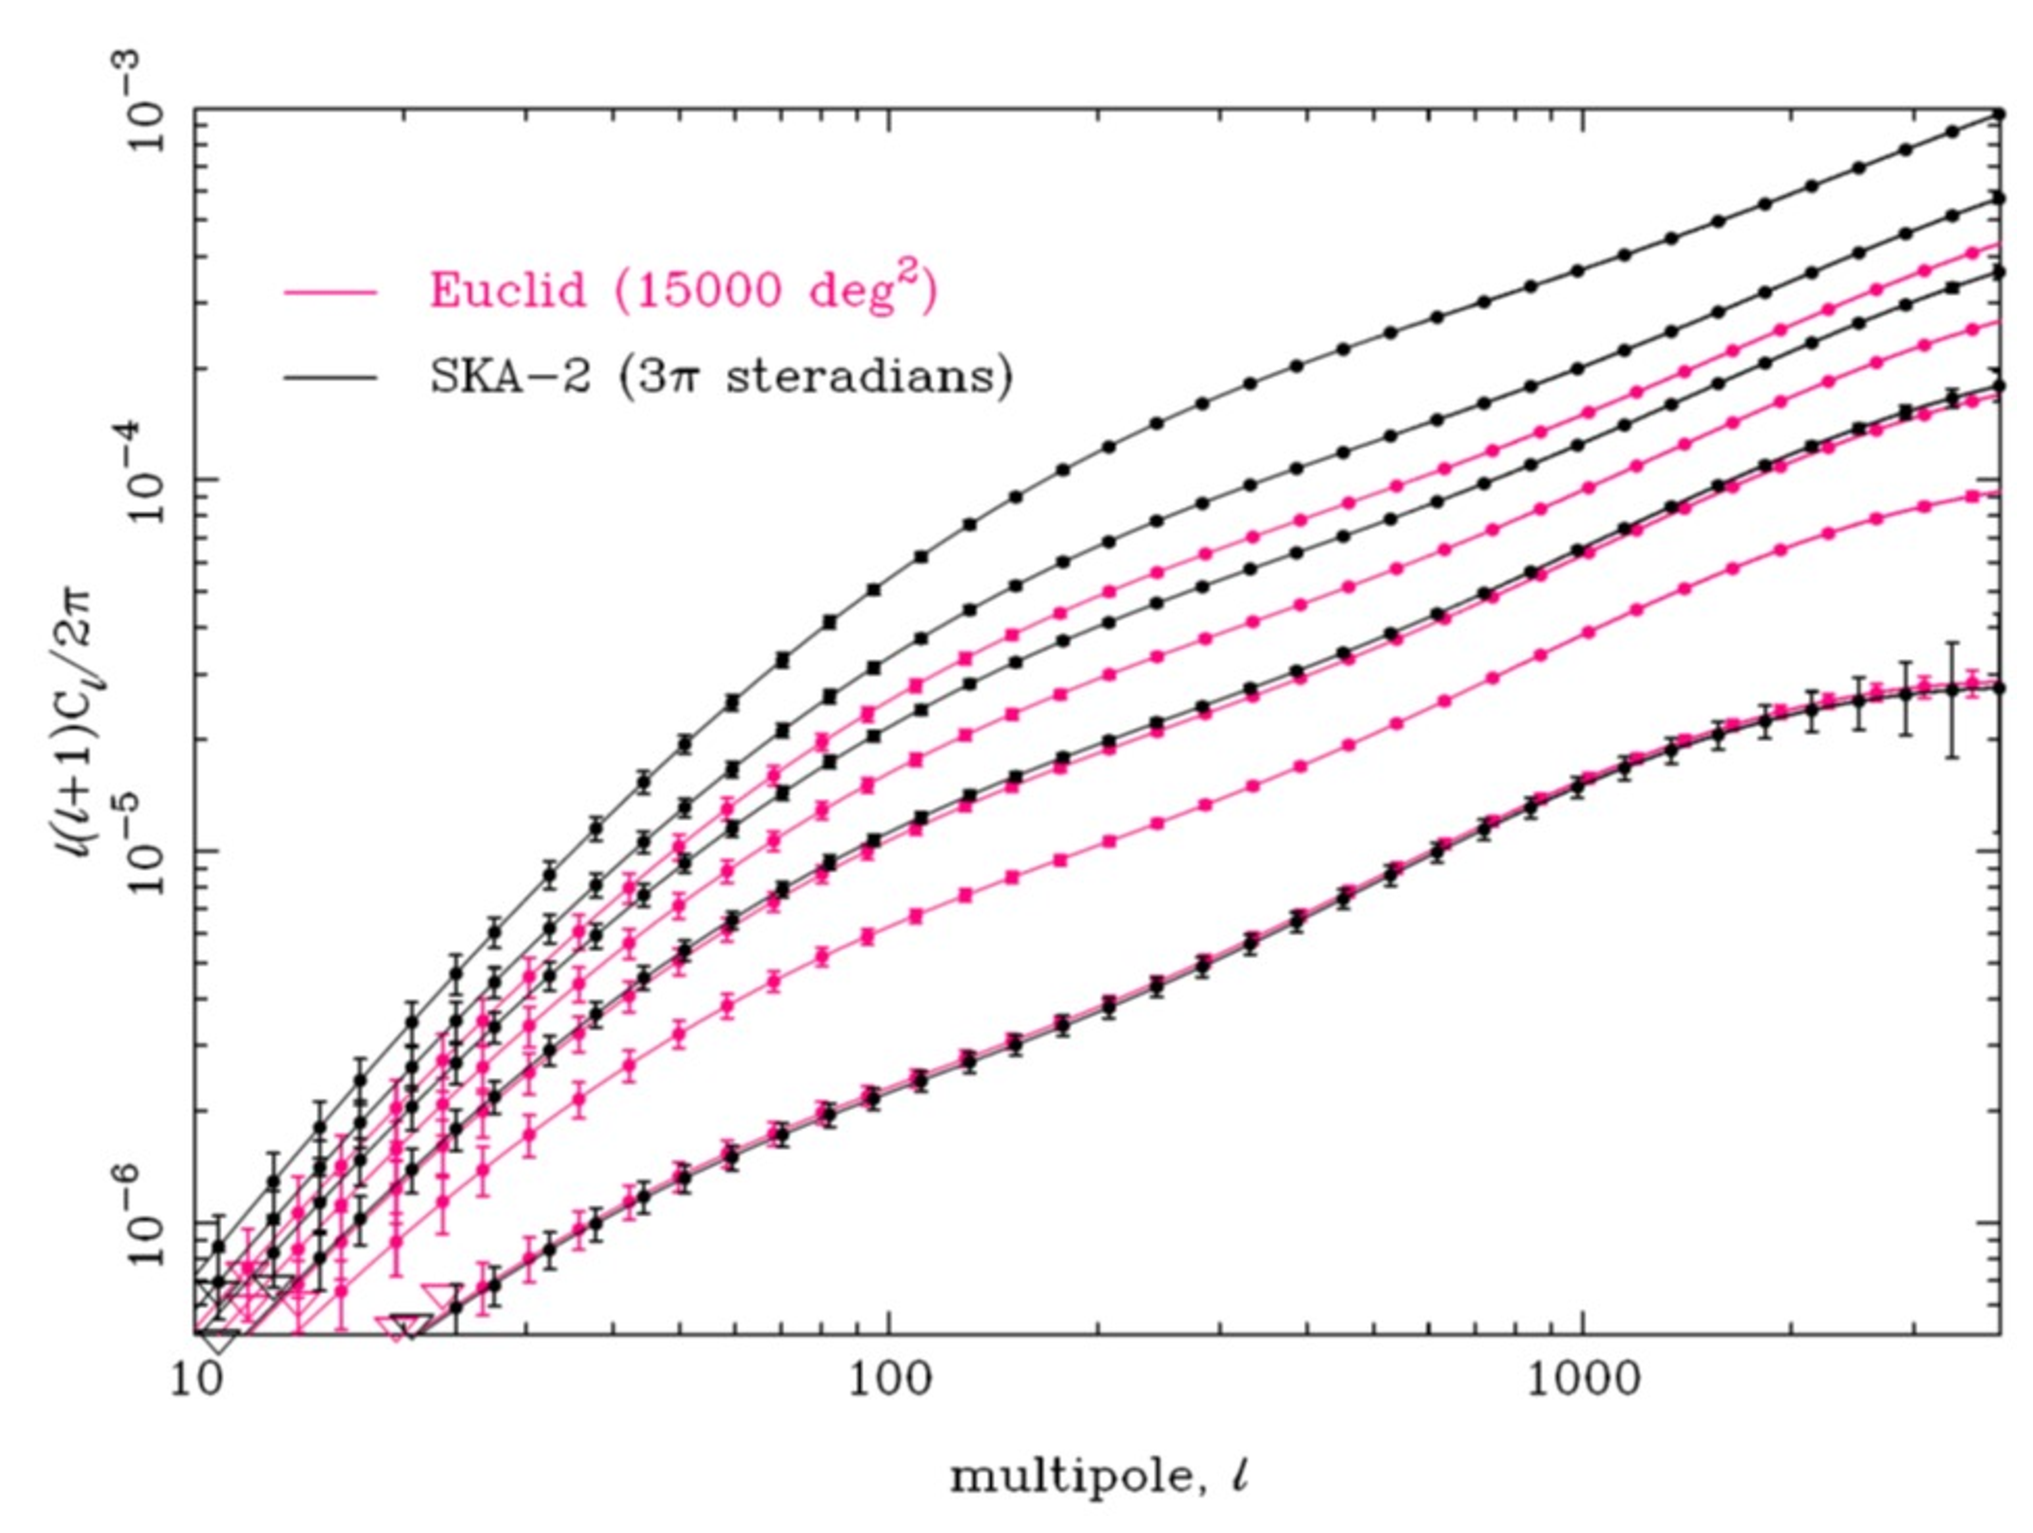
\includegraphics[width=1.0\linewidth]{cosmology/WL_power.eps} 
 \end{center}
 \end{minipage}
 \begin{minipage}{0.51\hsize}
 \begin{center}
   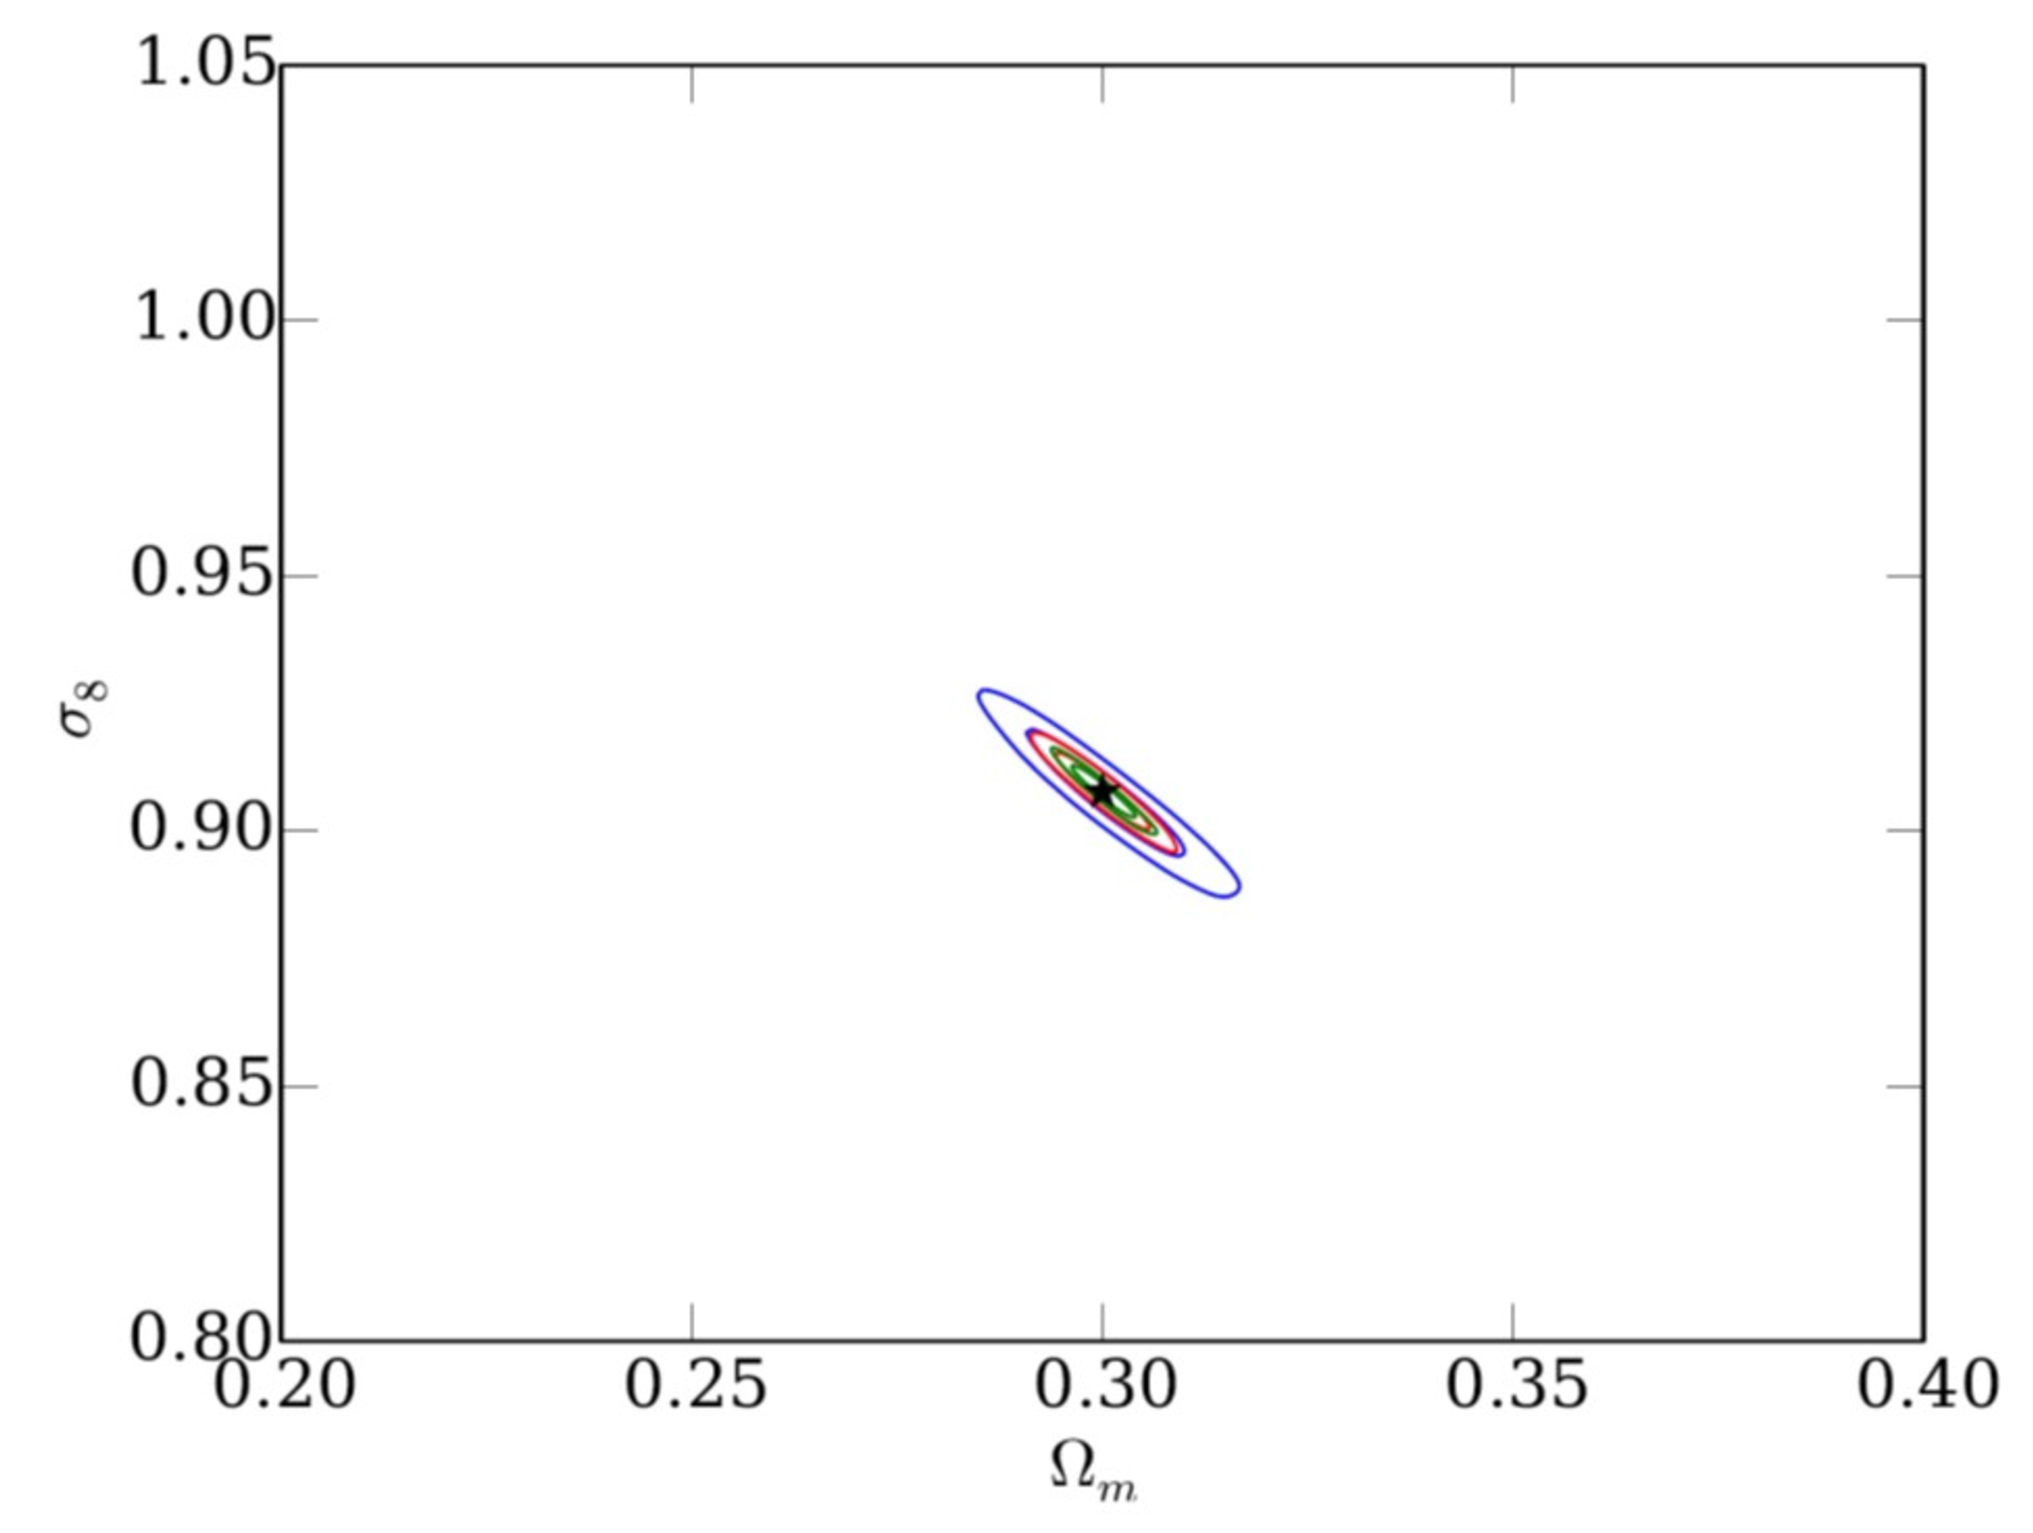
\includegraphics[width=1.0\linewidth]{cosmology/WL_constraint.eps} 
 \end{center}
 \end{minipage}
\caption{(左図) SKA2で期待される歪み場のパワースペクトルとその観測エラー
(各線は異なる赤方偏移におけるパワースペクトルであり、それぞれの実験に対し
赤方偏移ビンを$5$つに区切り、各赤方偏移ビンの幅は観測される銀河数が
同数になるように取られている。)。
比較のため、Euclidによる歪み場のパワースペクトルを赤線で示す。
(右図) SKA2の弱重力レンズ効果の観測を行った場合に期待される
$\Omega_{\rm m}$と$\sigma_{8}$の決定精度。
なお円の色の違いは観測する立体角の違いを表し、
それぞれ青線:$1000~{\rm deg}^2$、赤線:$5000~{\rm deg}^2$、緑線:$3\pi~{\rm steradian}$
の場合の制限である\citep{Brown:2015vqa}\label{fig:WL_fig1}。}
\end{figure}
%%%%%%%%%%%%%%%%%%%%%%%%%%%%%%%%%%%%%%%%%%%%%%%%%%%%%%%%%%%%%%%%%%%%%%%%%%%%
%%%%%%%%%Figure%%%%%%%%%%%%%%%%%%%%%%%%%%%%%%%%%%%%%%%%%%%%%%%%%%%%%%%%%%%%%
\begin{figure}[t]
 \begin{center}
%   \vspace{15pt}
   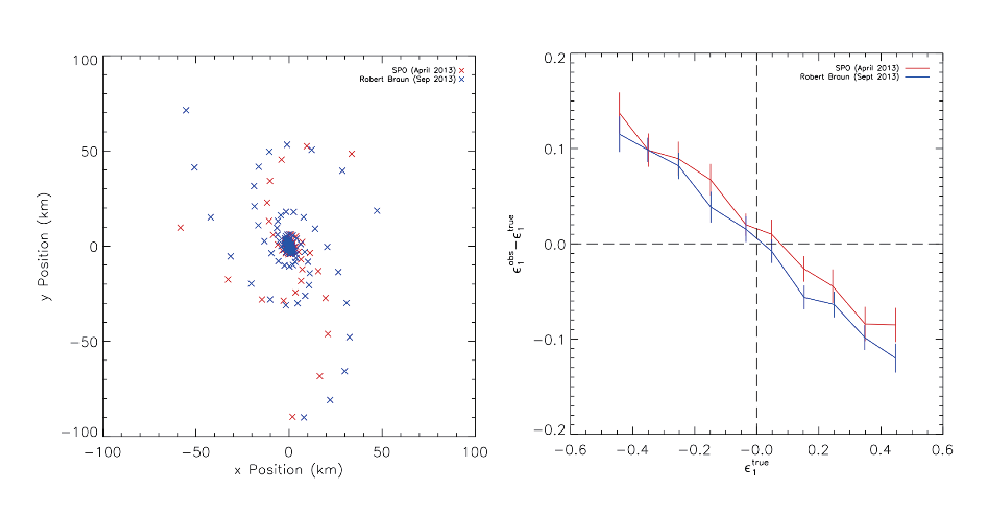
\includegraphics[width=0.95\linewidth]{cosmology/lensing_ellipse.eps} 
%   \vspace{10pt}
   \caption{SKAのアンテナ配置の違いによる、観測される銀河楕円率に生じる系統誤差の見積もり。
左図はアンテナの配置であり、右図は左図のそれぞれのアンテナ配置の場合に生じる
楕円率の系統誤差の大きさ(縦軸)を表す\cite{Patel:2015cra}。}\label{fig:weak_ellipse}
 \end{center}
\end{figure}
%%%%%%%%%%%%%%%%%%%%%%%%%%%%%%%%%%%%%%%%%%%%%%%%%%%%%%%%%%%%%%%%%%%%%%%%%%%%


また電波による弱重力レンズ効果の観測を行うことの利点として、
可視光観測との相関を取ることができるという点も挙げることが出来る。
例えば単一の観測(光学観測のみ等)によって測定された歪み場を$\gamma$とすると、
$\gamma$は重力レンズ起源の歪み場$\gamma_{\rm grav}$、その系統誤差$\gamma_{\rm sys}$
および銀河の固有の楕円率$\gamma_{\rm int}$によって
\begin{align}
	\gamma =\gamma_{\rm grav}+\gamma_{\rm int}+\gamma_{\rm sys}
	\,,
\end{align}
と表されるが、単にその自己相関を取った場合、
\begin{align}
	\langle\gamma\gamma\rangle
		=\langle\gamma_{\rm grav}\gamma_{\rm grav}\rangle
			+\langle\gamma_{\rm grav}\gamma_{\rm int}\rangle
			+\langle\gamma_{\rm int}\gamma_{\rm int}\rangle
			+\langle\gamma_{\rm sys}\gamma_{\rm sys}\rangle
	\,,
\end{align}
であり、系統誤差の寄与$\langle\gamma_{\rm sys}\gamma_{\rm sys}\rangle$が残ってしまうことになる。
次に電波観測と光学観測の間で相関を取ることを考えてみる。
電波観測による歪み場$\gamma^{(r)}$と光学観測による歪み場$\gamma^{(o)}$の間の相関を取ると
\begin{align}
	\langle\gamma^{(o)}\gamma^{(r)}\rangle
		=&\langle\gamma_{\rm grav}\gamma_{\rm grav}\rangle
			+\langle\gamma_{\rm grav}\gamma_{\rm int}^{(o)}\rangle
			+\langle\gamma_{\rm grav}\gamma_{\rm int}^{(r)}\rangle
			+\langle\gamma_{\rm int}^{(o)}\gamma_{\rm int}^{(r)}\rangle
			+\langle\gamma_{\rm sys}^{(o)}\gamma_{\rm sys}^{(r)}\rangle
	\notag\\
		=&\langle\gamma_{\rm grav}\gamma_{\rm grav}\rangle
			+\langle\gamma_{\rm grav}\gamma_{\rm int}^{(o)}\rangle
			+\langle\gamma_{\rm grav}\gamma_{\rm int}^{(r)}\rangle
			+\langle\gamma_{\rm int}^{(o)}\gamma_{\rm int}^{(r)}\rangle
	\,,
\end{align}
であり、第$5$項目の系統誤差の寄与を落とすことができる。
これは異なる実験間の系統誤差の間に相関がないということの結果である
($\langle\gamma_{\rm sys}^{(o)}\gamma_{\rm sys}^{(r)}\rangle =0$)。
また第$4$項である固有の楕円率の相関についても、電波と光学では放射機構が
異なるため、単一の観測のみの場合より小さくすることができる。
このように電波と可視光という異なる観測間で歪み場の相関を取ることによって、
両観測に存在する系統誤差等を取り除くことができるのである。
%その様な電波と可視光という異なる観測間で歪み場の相関を取ることによって、
%両観測に存在する系統誤差を取り除くことができるのである。
%
%

さらに電波観測においては、銀河の偏光の情報を利用できる
ということも大きな利点である。
%
銀河の弱重力レンズ効果を観測する上では、
銀河の元の楕円率の方向には相関が無いと仮定することで、
重力レンズによる楕円率の歪みの推定を行っている。
しかし実際には異なる銀河の楕円率の間には相関が存在しており、
その相関は系統誤差として影響を与える。
%
そこで、その元の銀河の楕円率の情報を得るために、
電波の偏光の情報を利用できるのではないかということが指摘されている。
この手法は銀河の元々の形状とその放射する電波の偏光との間に
相関が存在するため可能となる。
%
また銀河の回転軸と回転速度の観測を利用することで
元の銀河の方向を推定するという手法も提案されている。


%%%%%%%%%%%%%%%%%%%%%%%%%%%%%%%%%%%%%%%%%%%%%%%%%%%%%
\subsubsection{銀河楕円率推定のシミュレーション}
%
以上で説明した銀河の弱重力レンズ効果の観測においては、
ノイズの存在する観測データから、
銀河の形状(楕円率)を正確に推定することが重要となる。
%
そのため、銀河の楕円率を観測データから推定する解析手法の開発や、
電波干渉計のアンテナをどのように配置するのが、
銀河の楕円率を推定する上で最も効果的なのかについて、
詳細に調べていく必要が生じて来る。
%
そのことを目的とし、銀河の形状をインプットとして与え、
電波干渉計のアンテナ配置を様々に仮定した上で、
元の銀河の形をどの程度画像として正確に測定できるかについて
シミュレーションを行うという研究が現在行われている。
%
それらのシミュレーションでは、
アンテナ配置によって生じる系統誤差の大きさがどの程度になるのかについて
詳細に調べられており、そのシミュレーションによる結果の例が
図\ref{fig:weak_ellipse}の右図である。
% 
左図は計画されているSKAのアンテナの配置の一例で、
それぞれ赤と青の配置の場合に生じる系統誤差の影響が右図に示されている。
%
右図の縦軸はその系統誤差によって生じる
観測される銀河の楕円率の第1成分$\epsilon^{\rm obs}_{1}$と実際の銀河の楕円率$\epsilon^{\rm true}_{1}$の間の差を表している
(この図では楕円率の成分の内、片方の軸の成分のみ表示してある)。

今後、これら銀河の形状測定の妥当性がより詳細に検証されることが期待されており、
さらにこれらの手法を実際の電波干渉計のデータに用いることによる解析手法のテストについても、
将来のSKAによる弱重力レンズ効果の観測を目指して進展していくと予想される。



%%%%%%%%%%%%%%%%%%%%%%%%%%%%%%%%%%%%%%%%%%%%%%%%%%%%%%%%

\subsubsection{中性水素ガスの$21$cm線放射強度における重力レンズ効果}

これまでは銀河の形状に対する重力レンズ効果について述べてきたが、
さらにSKAではより大きな赤方偏移の時代
(宇宙再電離の時代から再電離が終わった後の時代にかけて)
を銀河間の中性水素ガスの$21$cm線輝線の観測によって
観測することが可能である。
したがって、その放射強度に対する弱重力レンズ効果についても
測定できると期待されている。
%
この観測における弱重力レンズ効果の測定手法は、
基本的にはCMBの重力レンズ効果観測における手法と同様であり、
歪み場の推定量を利用した統計的な解析を用いて、
弱重力レンズによる歪み場の測定を行うことが提案されてる。
%
この観測によって、銀河探査で観測できる時代より
さらに過去の密度揺らぎの情報を得ることが可能なため、
中性水素ガスの放射強度に対する弱重力レンズ効果の観測は、
暗黒エネルギーや修正重力理論の制限を目指す上で、
非常に有力な手法であると言うことができる。

%%%%%%%%%%%%%%%%%%%%%%%%%%%%%%%%%%%%%%%%%%%%%%%%%%%%

\bigskip

%%%%%%%%%%%%%%%%%%%%%%%%%%%%%%%%%%%%%%%%%%%%%%%%%%%%%
以上で説明してきた様に、
銀河の形状や中性水素の強度分布に対する弱重力レンズ効果の観測は、
SKAによる電波観測によって将来大きな進展が期待されており、
未だ詳細に調べられていない過去の宇宙を探査する上で、
非常に強力な観測手法となることが予想されている。



%%%%%%%%%%%%%%%%%%%%%%%%%%%%%%%%%%%%%%%%%%%%%%%%%%%%%%%%%%%%%%%%%%%%%%%%%%
\subsection{銀河団宇宙論}\label{cosmology.s2.ss7}
%%%%%%%%%%%%%%%%%%%%%%%%%%%%%%%%%%%%%%%%%%%%%%%%%%%%%%%%%%%%%%%%%%%%%%%%%%


%\subsubsection{Introduction}

中性水素$21$cm線は暗黒時代および再電離時期などを探るために
非常に有用な手段であることは様々に議論されているが~\citep{Pritchard:2011xb}、
ここでは、銀河団を用いた$21$cm線宇宙論について述べる。特に、銀河団による
スニヤエフ$\cdot$ゼルドヴィッチ(SZ)効果について考える~\citep{Colafrancesco2014}。

宇宙論的な$21$cm線放射が銀河団を通過する際、銀河団の中の
電子による逆コンプトン散乱で、そのスペクトルは変更を受ける。
これは、CMBでよく議論されているSZ効果であるが、
ここでは、特にこの宇宙論的な$21$cm線放射のスペクトルに関するこの効果を
SZ-$21$cm効果と呼ぶことにする。 

CMBの光子は銀河間物質を通過してくる際、
暗黒時代から、初代天体形成、再電離の時期において、
ガスとの衝突結合による吸収、
ライマン-$\alpha$、X線放射などにより、そのスペクトルは変更を受ける。
$I_0 (\nu)$ をCMBのスペクトルとし、
このスペクトルが銀河間物質を通過した後 $\widetilde{I}(\nu)$ に変更されたとすると、
宇宙論的な$21$cm線放射の(CMBに対する)輝度温度 $\delta T (\nu)$ は
\begin{equation}
%\label{ }
\delta T (\nu)
= \frac{c^2}{2 k_{\rm B} \nu^2} \left( \widetilde{I} (\nu) - I_0 (\nu) \right) 
= \frac{c^2}{2 k_{\rm B} \nu^2} \delta I (\nu)
\end{equation}
と書ける。ただし、ここでは レイリー$\cdot$ジーンズ周波数領域を考えている。

SZ-21cm効果は $\widetilde{I} (\nu)$ と $I_0 (\nu)$ それぞれに対するスニヤエフ$\cdot$ゼルドヴィッチ
効果の差として見ることができる。初期スペクトルが$\widetilde{I}(\nu) $ の放射について、
銀河団中の電子による逆コンプトン散乱の後、SZ効果によって変更されたスペクトルは
以下のように書ける~\citep{Cooray:2005bc}:
\begin{equation}
%\label{ }
\widetilde{I}_{\rm mod} (\nu) = \int_0^{\infty} d \nu_0 P_\tau (\nu, \nu_0) \widetilde{I} (\nu) 
\end{equation}
ここで、$P_\tau (\nu, \nu_0)$は振動数が$\nu_0$の光子が振動数$\nu$になる
確率を表す分布関数であり、散乱断面積、電子の分布関数、銀河団の光学的深さなどにより計算される。
特に一回の散乱による確率分布関数を$P_1(\nu, \nu_0)$とすると、光学的深さ$\tau$の銀河団を
通過した際は $P_\tau (\nu, \nu_0) = (1-\tau) \delta (\nu - \nu_0) + \tau P_1 (\nu, \nu_0)$と書ける
(ただし $\tau \ll 1$ とする)。
今考えているSZ-21cm効果は
\begin{equation}
\label{eq:SZE21cm}
\Delta I_{\rm mod} (\nu) = \widetilde{I}_{\rm mod} (\nu) - \widetilde{I} (\nu)
\end{equation}
に相当する。
電子が熱的、非熱的な分布をしている場合、それぞれを熱的SZ効果、非熱的SZ効果と呼ぶ。
%図\ref{fig:brightnessT}では熱的SZ効果の場合の振動数スペクトルが描かれている。

\subsubsection{SZ効果と$21$cm線}

ここでは実際の周波数スペクトルの理論予言について見てみる~\citep{Colafrancesco2014,Cooray:2005bc}。
図~\ref{fig:brightnessT}の左図はCMB放射に対する21cmの輝度温度で、
右図はその放射がさらに銀河団による熱的SZ効果を受けた後のスペクトルを示している。

まず、左図の輝度温度について、スペクトルの特徴的な振動数に着目して見てみる。
まず、$ 30 < z <200$ では衝突結合による吸収があり、
これに対応して$\nu \sim 20$~MHz を中心として、輝度温度が負になっている。
また、$ 20 <z <30$での初代天体からの ライマン-$\alpha$放射場による
吸収が $\nu\sim 70$~MHz で見られる。
そして、その後$z<20$での軟X線加熱により、$\nu\gtrsim 100\,$MHzで輝度温度が正に大きくなっている。

右図は左図のスペクトルと、そのスペクトルが銀河団による熱的SZ効果
を受けたあとのスペクトルとの差を取ったものである (\eqref{eq:SZE21cm}式に対応)。
このスペクトルも左図と同様に特徴的な振動数依存性があることがわかる。
特に、$\nu\sim 60$ MHzにライマン-$\alpha$放射場との相互作用による負のピークを持つが、
$z\sim 20$にライマン-$\alpha$の急激な吸収が起こることで$\nu\sim 70$ MHzに
正のピークを生成する。
右図のスペクトルを$21$cm線の観測で見る事ができれば、
銀河団サーベイに対して非常に有用である。
また、それらの銀河団の情報を通じて暗黒時代および再電離時期に関する情報が得られる。

また、図~\ref{fig:brightnessT}では熱的SZ効果によるものであるが、
同様にして非熱的な電子分布による非熱的SZ効果の場合の
振動数スペクトルも計算することができる~\citep{Colafrancesco2014}。
この非熱的SZ効果の方がその差$\Delta I_{\rm mod}$ は小さくなるが
(輝度温度$\delta T$ で$1/40$程度の大きさになる~\citep{Colafrancesco2014})、
そのスペクトルの形は熱的なものと異なるため、原理的にはそのスペクトルの違いに
より区別ができ、銀河団等の電子分布の情報を得る事ができる。

%%%%%%%%%Figure%%%%%%%%%%%%%%%%%%%%%%%%%%%%%%%%%%%%%%%%%%%%%%%%%%%%%%%%%%%%%
\begin{figure}[t]
 \begin{minipage}{0.5\hsize}
 \begin{center}
%   \vspace{15pt}
   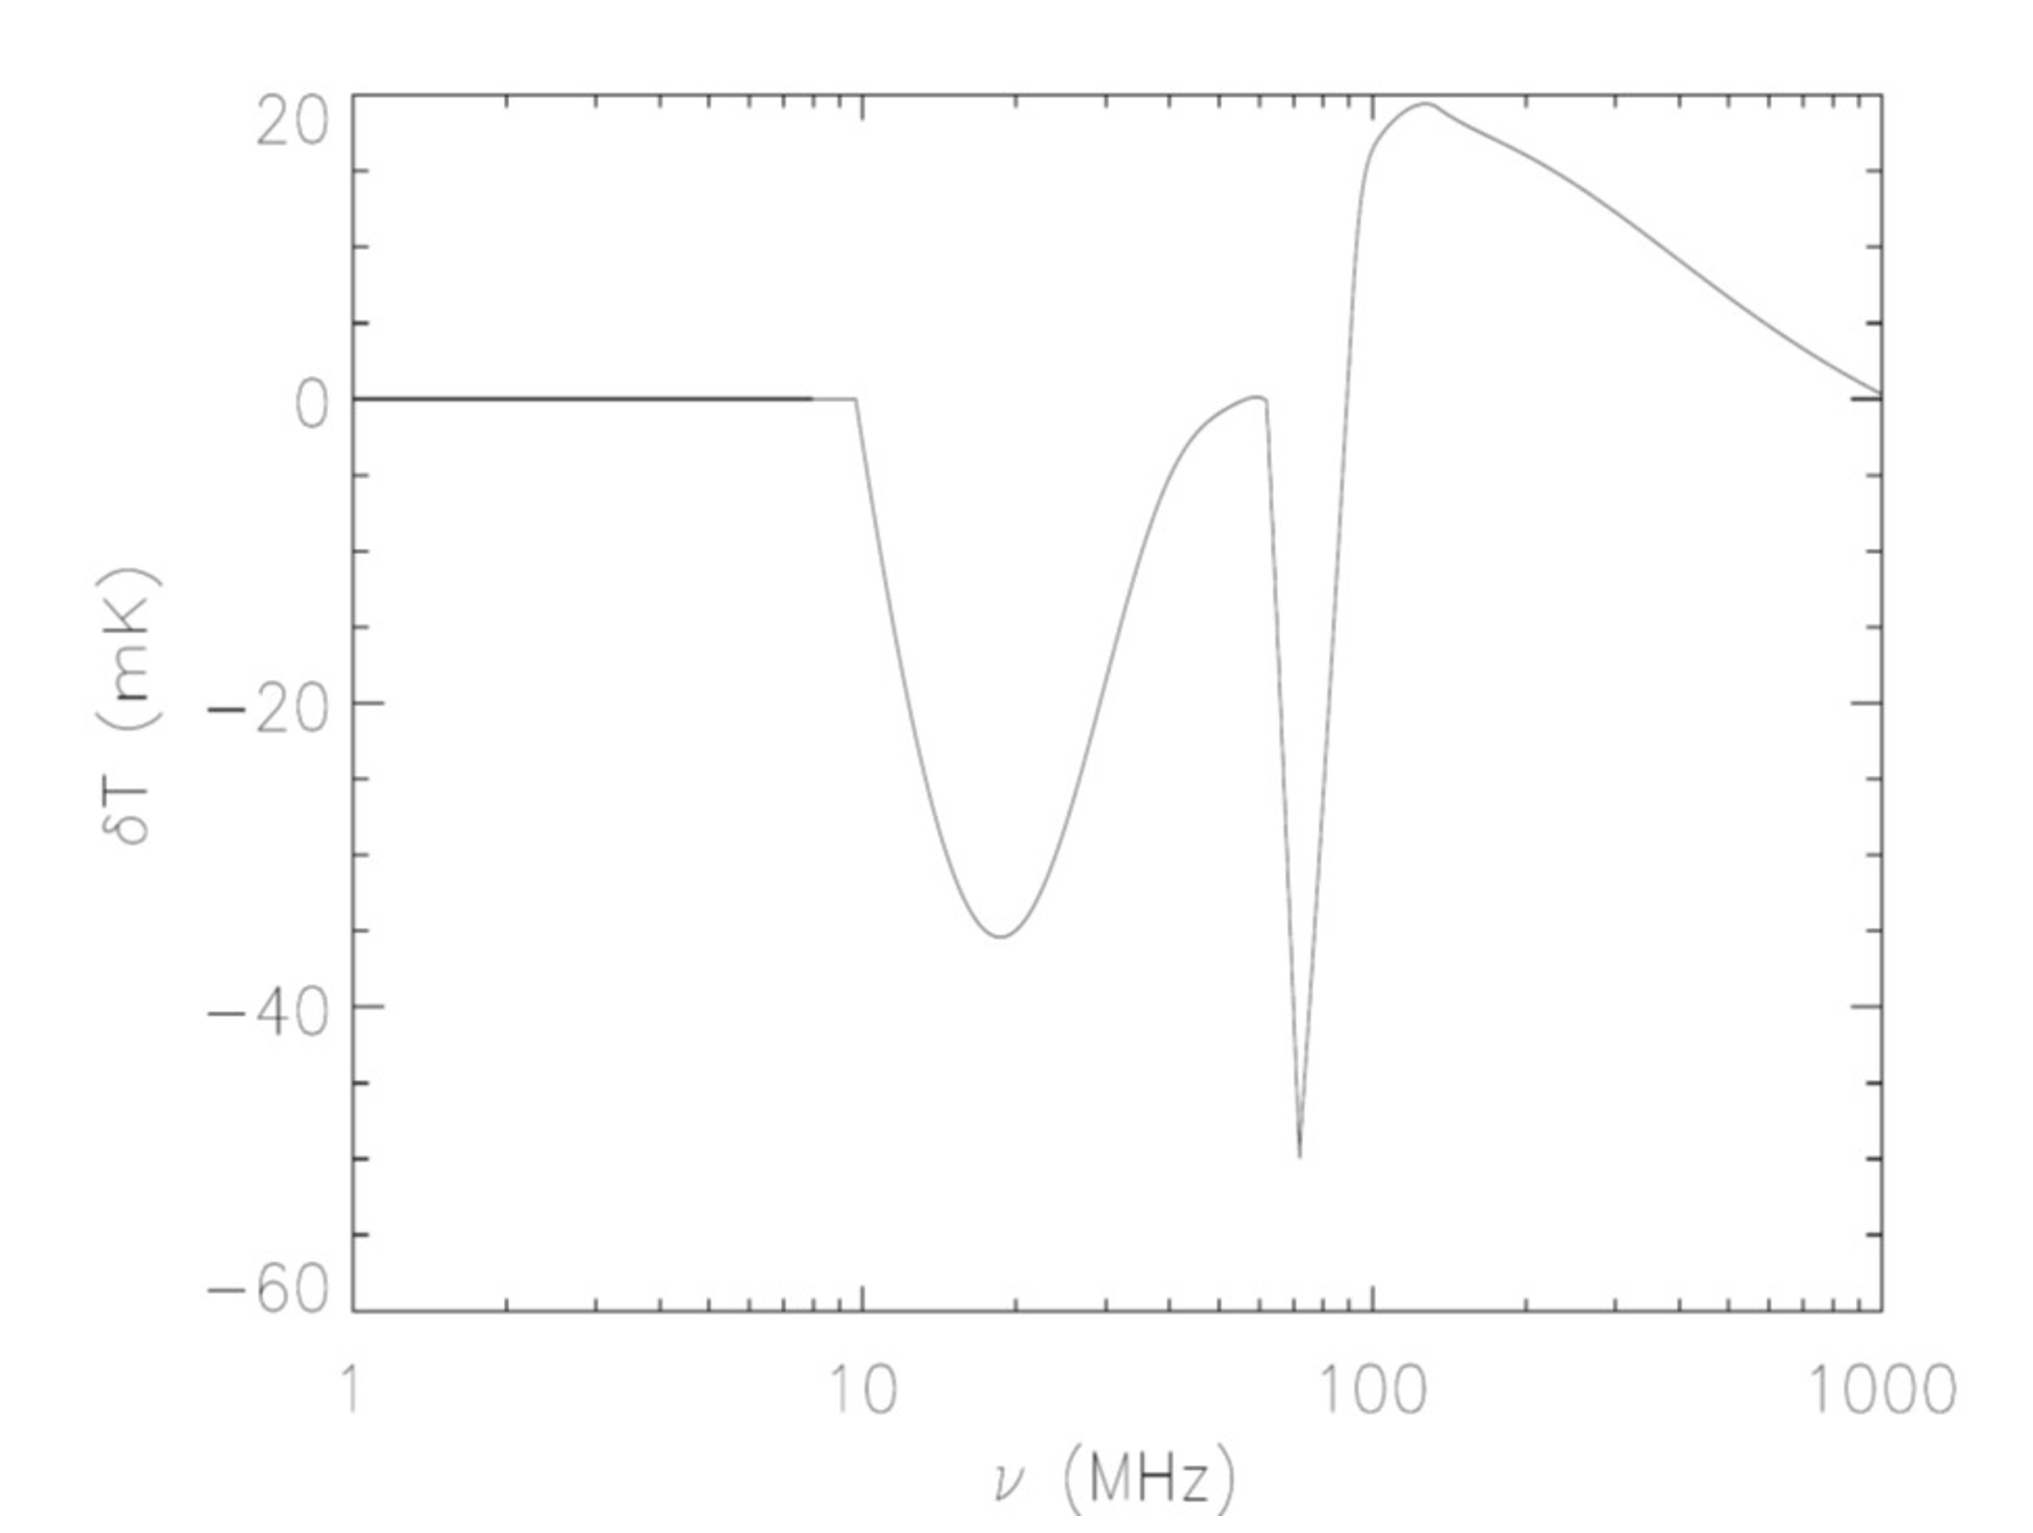
\includegraphics[width=1.0\linewidth]{cosmology/cluster_21cm.eps} 
%   \vspace{10pt}
 \end{center}
 \end{minipage}
 \begin{minipage}{0.5\hsize}
 \begin{center}
   \includegraphics[width=1.0\linewidth]{cosmology/cluster_SZ-21cm.eps} 
%  \vspace{-15pt} 
 \end{center}
 \end{minipage}
\caption{(左図) CMB放射に対する輝度温度の周波数スペクトル。
(右図) 熱的SZ効果を受けた輝度温度スペクトルと受ける前のスペクトルの差。
熱的プラズマ温度はそれぞれ$kT = 5$ (solid) $10$ (dashed), $15$ (dotdashed), $20$ (dash-three dots) ${\rm keV}$
であり、光学的深さは$\tau =5\times 10^{-3}$としている\citep{Colafrancesco2014}。}
\label{fig:brightnessT} 
\end{figure}
%%%%%%%%%%%%%%%%%%%%%%%%%%%%%%%%%%%%%%%%%%%%%%%%%%%%%%%%%%%%%%%%%%%%%%%%%%%%


\subsubsection{SKAを用いた銀河団探査}

図~\ref{fig:brightnessT}より、熱的SZ-$21$cm効果のシグナルは振動数$300$~MHz以下で
大きくなることが分かる。
これは丁度SKA1-LOW ($50$--$250$~MHz) の振動数領域であり、
熱的SZ-$21$cm効果を観測するのに適していると言える。
実際、SZ-$21$cm効果を用いることで$\nu\sim 70$ MHzにおいては$kT\sim 20\,{\rm keV}$程度の
高温の銀河団、また、より高振動数側で感度が高くなるため、
$\nu\sim 90$ MHzにおいては比較的低温($kT\sim 5\,{\rm keV}$)程度の銀河団も
観測しうる。
一方、非熱的SZ-$21$cm効果のシグナルは(大きさは小さいものの)
SKA1-MID band 1 ($350$--$1050$~MHz) の方まで多少伸びているため、
このバンドでの観測可能性も興味深い。
これらのSZ-21cm効果のスペクトルを観測することにより、
対応する赤方偏移での暗黒時代、再電離時期を探査できる。

上記では、SZ-$21$cm効果を用いた暗黒時代、再電離時期の探査について述べたが、
銀河団を用いた宇宙論に関連するテーマとして、
ニュートリノ質量、暗黒エネルギー、修正重力理論、原始非ガウス性
なども議論できるであろう。



%%%%%%%%%%%%%%%%%%%%%%%%%%%%%%%%%%%%%%%%%%%%%%%%%%%%%%%%%%%%%%%%%%%%%%%%%%
\subsection{宇宙原理}\label{cosmology.s2.ss8}
%%%%%%%%%%%%%%%%%%%%%%%%%%%%%%%%%%%%%%%%%%%%%%%%%%%%%%%%%%%%%%%%%%%%%%%%%%

「我々の宇宙は空間的に一様かつ等方である」という宇宙原理の検証を高赤方偏移で
実現する可能性をSKAは秘めている。

現在の標準宇宙モデルに組み込まれつつあるインフレーション理論(\ref{cosmology.s1.ss1}節)において、
大きなスケールでの一様等方性は重要な予言である。インフレーション理論は、背景宇宙の
一様等方性を予言するだけでなく、CMBの温度揺らぎや、宇宙大規模構造の種となる初期密度揺らぎの起源を自然に説明できる。
そして、その予言される初期密度揺らぎの統計的性質は、ほぼガウス分布に従い、統計的に等方である、というものである。
さて、この宇宙原理の検証において、等方性の検証に比べ、一様性の検証はそれほど容易ではない~\citep{Ichiki:2014rua}。
CMB観測で温度がほぼ等方であることなどから、等方性は検証される。
さらに、CMB観測は、その温度揺らぎと偏光の情報からインフレーション理論を強く支持している。
しかし、
実は、すでにCMB観測で非常に大きなスケールでアノーマリーが見えているのでは、という議論があがっている。
温度揺らぎのパワーの大スケールでの欠損、そのパワーの双極子的な変調やパリティの非対称性などである。
これらアノーマリーが真に存在するのであれば、インフレーションを含めた標準宇宙モデルの変更を余儀なくされる。
よって、宇宙の一様等方性に関連した、これら非常に大きなスケールでのアノーマリーの精密な検証は、非常に重要である。
観測的には、CMBに比べ、SKAでは数多くの独立なモードを見ることが出来る。
大きなスケールに関して言えば、赤方偏移$z=O(1)$での超地平線のモードも見ることが可能である。
宇宙原理に関しては、例えばCMBと大規模構造の静止系が超地平線モードによって一致しない
可能性の検証が、SKAでは可能である~\citep{Schwarz:2015pqa}。

\subsubsection{宇宙論的な電波双極子} 

CMBにおけるダイポール(双極子)成分は、我々の固有運動のせいであると一般的には
「仮定」される。これにより、基準となるフレームを決めることになる。
しかし、厳密には運動起源の双極子なのか、他の物理現象からの双極子的寄与なのかを
CMBでは区別することが難しい。
すでに、電波観測で見られる双極子成分に対する制限は、NVSSやWENSSといった
電波源カタログから得られているが、いまだ誤差は大きい。CMB側では、
近年Planckチームにより、大きな多重極モーメントでも
ドップラーシフトの影響を発見したという報告もあったが、それほど精度が高いものでもない。
CMBの双極子成分の方向$\vec{d}_{\rm CMB}$と、電波源の双極子方向$\vec{d}_{\rm radio}$との
比較やその大きさ自体への制限にも、SKAの超地平線にわたる大きな体積での観測
が有効であると期待される。
具体的には、$< 1\,{\rm GHz}$の低周波数帯で連続波サーベイが有効であるが、
Early Science phaseで電波双極子の測定には十分である。

\subsubsection{大角度スケール}

運動学的起源の非等方性ではなく、時空そのものの等方性についての議論も、大きな角度スケールの観測により可能となる。
例えば、CMB観測では四重極と八重極揺らぎのパターン方向がそろっているなどのアノーマリーが報告されている。
SKAによる電波観測とCMB観測を組み合わせることで、観測されるCMB温度揺らぎを、最終散乱面で作られた成分と、
その後我々までに届く間に生まれた成分(例えば積分ザックス・ボルフェ効果)とに
分離できることが期待され、それによりアノーマリーの起源により詳細に迫ることが出来ると考えられる。

\begin{itemize}

\item 低い$\ell$多重極モーメント

これらアノーマリーに迫るためには、やはり大スケール、
つまり低$\ell$多重極モーメントの
精査が必要となる。図\ref{fig:low-ell}は、SKA1連続波サーベイで期待されるSKA銀河の角度パワースペクトルを誤差付きで表している。

\begin{figure}[tbp]\label{fig:fig.eps}
\begin{center}
\includegraphics[width=0.6\linewidth]{cosmology/foundation_fig.eps}
\end{center}
\caption{SKA1連続波サーベイで期待されるSKA銀河の角度パワースペクトルとその観測誤差。}
  \label{fig:low-ell}
\end{figure}

\item 角度$2$点相関

大規模構造の分布を解析する際に、角度$2$点相関関数も有力な手法である。
原始揺らぎの非ガウス性への制限などにも角度$2$点相関関数は用いられている。
アノーマリーとは少し離れるが、大スケールの$2$点相関関数には、相対論的効果が
表れるという指摘もあり、とくに赤方偏移が分かるHI銀河赤方偏移サーベイにより、
この相対論的効果の検証も可能であると考えられる。

\end{itemize}

\subsubsection{コペルニクス原理と一様性}

コペルニクス原理とは、「我々がいる場所は宇宙の特別な空間ではない」というものである。
宇宙の等方性がわかって、この原理に従えば、宇宙の一様性が言えることになる。
コペルニクス原理の検証は、暗黒エネルギーの解明とも関連する。
宇宙が加速膨張していることを示唆する現在の観測結果を実現する
ためには、暗黒エネルギーの存在が不可欠であるがそれは一様性を仮定した時である。
コペルニクス原理が破れていて、我々が大きなボイド空間の中心にいても
宇宙が加速膨張しているように見える状況を作り出すことができるということも示唆されているが、
様々な観測との整合性を考えるとこのボイドモデルはあまりうまくいっていない。
しかし、その原理の検証をさらに詳細に行うことは重要である。
一様か一様でないかのチェックとして、
\begin{equation}
{\mathcal C}(z) = 1 + \widetilde h^2\left( DD'' - {D'}^2\right) + \widetilde h\widetilde h' DD' = 0
\end{equation}
という式を用いることができる~\citep{Clarkson:2007pz}。ここで、$\widetilde h= H(z) / H_0 $、$D(z)$
は共動距離を表し、また$' = d/dz$である。
${\mathcal C}(z) \neq 0$でコペルニクス原理が破れていることを表す。
SKA1では、$z<1.5$の観測データを用いて$\sigma ({\mathcal C}(z)) =0.05$まで到達可能であると期待される。
\\

現代の宇宙論は、飛躍的な観測技術の進歩により、精密科学の域にまで達している。
今後は、これまで仮定としていた宇宙の一様性、等方性という宇宙論の基礎の検証も出来ると考えられている。
CMB観測と合わせて、SKAによる電波観測もその有力な道具の一つとして期待される。




\section{日本が狙うサイエンス}\label{cosmology.s3}

この章では、SKA計画で注目される宇宙論研究について我が国で進展が期待される科学的な課題について
以下にまとめる。

\ref{cosmology.s1.ss1}節で述べたように、現在我々が直面する宇宙論の重要な未解決問題は大きく
次の3つである:「インフレーションがどのように起こったのか」、「暗黒エネルギーの正体とは何か」、
「暗黒物質の正体は何か」である。
SKAのような低周波電波干渉計により、$30,000$平方度にわたる広範な天球を掃くだけでなく、
$z\gtrsim 5$のような高赤方偏移宇宙にまで到達可能であることから、
SKAの観測データを用いることでこれまでにない精度・規模の宇宙論観測が可能になる。

しかしその一方で、上記のような問題にアプローチしうるような精密宇宙論探査を
観測データから行うことは容易なことではない。
近傍宇宙では密度揺らぎは十分成長しており、
小スケールにおいて非線形性を無視することができなくなる。
非線形発展する系において精密な理論予言を行うことは非常に困難である。
近年多くの高精度$N$体計算や解析模型が提唱されているが、
常にモデルの自由度を内在することになってしまう。
さらに、小スケールではバリオンの物理を含む宇宙物理的な過程が介在することから
精密な予言を行うことを難しくしている。
これらの問題を打破し、そして宇宙論の未解決問題に決定打を与えるため、
SKA-JP宇宙論班では以下の3つを大きな活動の柱とする。
\begin{itemize}
\item[] (i) 超地平線スケール宇宙論によるインフレーション・暗黒エネルギーの探求
\item[] (ii) $21$cm線サーベイを用いた暗黒宇宙探査
\item[] (iii) 精緻な理論模型構築と暗黒エネルギー
\end{itemize}
それぞれは有機的に密接に関連しており、関係は相補的である。
以下、それぞれについて、研究の現状および問題点、研究計画を列挙する。\\

\begin{enumerate}
\item[{\bf (i)}] {\bf 超地平線スケール宇宙論}

上述の問題を打破する一つの方法は、地平線スケールを超えるような大スケールを探査することである。
超地平線スケールでは、密度揺らぎが線形領域に留まるだけでなく、
主たる宇宙物理的過程も介在しないことから非常にクリーンな理論予言が可能となる。
このとき、最大の障害となるのは宇宙の単一性により独立なモードを十分に取得することができず、
有限のサンプル数によるノイズ:コズミックバリアンス(Cosmic Variance; CV)を生む。
よって、SKAのようなほぼ全体を覆う広範な観測領域を持つ場合、CVを適切に取り扱うことが不可欠である。
我々宇宙論班は、コズミックバリアンスを取り扱う最も有望な手法として、
マルチトレーサー法~\citep{Seljak:2008xr}を積極的に取り入れることで、
観測データから宇宙論における有用な情報を効率的に抜き出すことを計画している。
この手法では、一つの観測データを少なくとも二つ以上の異なるバイアス因子を持つような
グループに分割することが本質的である。
複数のグループの相互相関を計算することで、バイアスの比の決定精度をショットノイズだけに
依存するようにすることができる。
これにより実効的にCVに依らずに観測量を制限することができる。
この手法の大きな利点としては、バイアスに依存する観測量であれば、観測量の如何に依存せずその効果を発揮する点である。
そのため、一つの手法で様々な宇宙論的諸問題に迫っていくことができる。

\begin{description}
\item {\bf 原始非ガウス性}

%宇宙最初期の指数関数的膨張期、いわゆるインフレーションがどのように起こったのかは現在においてもなお
%明らかになっておらず、宇宙論分野における最も重要な研究テーマの一つである。
インフレーションを決定付ける最後のピースは
%近年注目されているのは、宇宙大規模構造の種、つまり
インフレーションが導く原始揺らぎの統計性の検定である。
最もシンプルなインフレーション模型が
ほとんどガウス統計に従う揺らぎを生成することは以前より知られていた。
しかし、高エネルギー物理の理解が深まるにつれ、ガウス統計から大きく逸脱した揺らぎを生成するような模型の
存在が認知されている。
原始非ガウス性は模型に固有の理論予言を与えることから、あまた存在するインフレーション模型の選別に用いることができる。
この理論的研究は宇宙論班に在籍する研究者を含む多くの日本人が重要な寄与をしてきたという
実績があり、観測への応用においてもその素地を生かすことで大きな貢献が見込める。

既に\ref{cosmology.s1.ss1}節で議論したように、\eqref{eq:fNL def}式のように特徴づけるのが一般的である。
既に非線形パラメータ$f_{\rm NL}$に対して様々な観測から制限が与えられているが、
%既にPlanck衛星によるCMBの観測により、$f_{\rm NL}=2.7\pm 5.8$ ($68\%$ C.L.)という制限値が与えられている。
最もシンプルなインフレーション模型は$f_{\rm NL}={\cal O}(0.01)$という非常に小さい値を予言することから、
誤差を${\cal O}(0.01)$に抑えることが今後の宇宙論研究において重要な地位を占めることになる。
原始非ガウス性が存在する場合には、%銀河数密度揺らぎの背景にある暗黒物質揺らぎに対する
バイアスがスケールおよび赤方偏移依存性を持つことが近年指摘されており (\eqref{eq:scale dependent bias}式)、
銀河サーベイを用いてバイアスのスケール依存性を精密に測定することで原始非ガウス性を観測することができる。
CMBを用いた場合、将来観測であっても$\sigma (f_{\rm NL})={\cal O}(1)$までにしか到達できないのに対し、
SKAではこの観測の壁を越えてインフレーション模型に迫っていける可能性がある。

宇宙論班の山内、大栗、高橋によって、マルチトレーサー法をSKA連続波サーベイに応用することにより、
原始非ガウス性を探査する研究を既に実施し、論文としてまとめている~\citep{Yamauchi:2014ioa}。
実際的な観測に含まれる系統誤差を考慮に入れた場合であっても、マルチトレーサー法により
決定誤差を大きく抑制できることを明らかにし(図~\ref{fig:sigma_fNL_multitracer}左図)、
SKA連続波サーベイにより、CMBよりも強い制限$\sigma (f_{\rm NL})\lesssim 1$を得ることができることを示した。
さらに、光赤外観測計画Euclidとの結合解析により、$\sigma (f_{\rm NL})\approx 0.5$にまで到達しうることを
初めて示した実績がある (図~\ref{fig:sigma_fNL_multitracer}右図)。
この論文では、SKA連続波探査単体では銀河の赤方偏移については情報が得られないとして、最も悲観的な状況での
解析を行った。
しかし、%赤方偏移の情報の重要性についても議論しており、
光赤外観測との協働によりSKAで見出した銀河に赤方偏移情報を付与することで状況はさらに改善し、
$\sigma (f_{\rm NL})=0.01$を目指すことができる~\citep{Kitching:2015fra,Takahashi:2015zqa}。


%%%%%%%%%Figure%%%%%%%%%%%%%%%%%%%%%%%%%%%%%%%%%%%%%%%%%%%%%%%%%%%%%%%%%%%%%
\begin{figure}[t]
 \begin{minipage}{0.52\hsize}
 \begin{center}
%   \vspace{15pt}
   \includegraphics[width=1.0\linewidth]{cosmology/sigma_fNL_nTracer.eps} 
%   \vspace{10pt}
 \end{center}
 \end{minipage}
 \begin{minipage}{0.52\hsize}
 \begin{center}
   \includegraphics[width=1.0\linewidth]{cosmology/sigma_fNL_survey.eps} 
%  \vspace{-15pt}
 \end{center}
 \end{minipage}
\caption{(左図) トレーサーの分割数に対する非線形パラメータ$f_{\rm NL}$の決定精度。
%マルチトレーサー法を用いた結果、トレーサーを分割すればするほど実際にバイアスに含まれる
%原始非ガウス性の決定誤差が小さくなることを確認することができる。
(右図) サーベイ計画ごとの$f_{\rm NL}$の決定精度。
Euclidについては観測データから銀河質量を推定できるため、自由にトレーサーを分割できるとしているが、
SKAは銀河の形状タイプごとに分割し、それぞれに質量の推定値を付与することでバイアスを与えている。
\label{fig:sigma_fNL_multitracer}}
\end{figure}
%%%%%%%%%%%%%%%%%%%%%%%%%%%%%%%%%%%%%%%%%%%%%%%%%%%%%%%%%%%%%%%%%%%%%%%%%%%%
%<><><><><><><><><><><><><><><><><><><><><><><><><><><><><><><><><><><><><><><><><><><><><><><><><><>%
\begin{figure*}
\begin{center}
\includegraphics[width=100mm,clip]{cosmology/sigma_fNL_future.eps}
\caption{
SKAを用いた原始非ガウス性の探査における将来展望。
}
\label{fig:sigma_fNL_future}
\end{center}
\end{figure*}
%<><><><><><><><><><><><><><><><><><><><><><><><><><><><><><><><><><><><><><><><><><><><><><><><><><>%

この結果を踏まえ、SKA-JP宇宙論班として、
マルチトレーサー法を用いた原始非ガウス性の探査を行う。
以下より具体的な研究計画を以下に示す。

まず第一に我々は、より広いクラスの非線形パラメータに着目する。
原始非ガウス性は多点相関関数の形状に依存するため、上述したパラメータ$f_{\rm NL}$以外にも
多数のパラメータが存在することが知られている。
これらを網羅的に調べなければ、原始非ガウス性の全貌を明らかにすることはできない。
$f_{\rm NL}$以外の原始非ガウス性を探査する重要な点として、無矛盾条件の存在が挙げられる。
原始揺らぎが単一の場によって生成されるインフレーション模型を考えた場合、$f_{\rm NL}$と$4$点関数を特徴付ける
非線形パラメータ$\tau_{\rm NL}$の間に以下の関係が成立することが知られている~\citep{Boubekeur:2005fj,Okamoto:2002ik}:
\begin{align}
	\tau_{\rm NL}=\frac{36}{25}\left( f_{\rm NL}\right)^2
	\,.\label{eq:condition}
\end{align}
この無矛盾条件の可否を調べるためには、高次効果を適切に観測データから読み取る必要がある。
それは容易なことではないが、得られる情報は多岐にわたる。
無矛盾条件の破れを観測から見出した場合にはインフレーション模型に対する重要な示唆を与える。
特に、破れの原因として、インフレーションが複数の場によって引き起こされた可能性が盛んに議論されている。
最も単純なインフレーション模型は、質量の軽い単一のスカラー場により引き起こされるものであるが、
高エネルギー物理の観点に立った場合、宇宙初期に軽質量スカラー場がただの一つしかないことは不自然であり、
一般的には複数場が同時に揺らぎに寄与しうる(例えば\cite{Lyth:2001nq,Moroi:2001ct,Enqvist:2001zp})。
その際には上記の無矛盾条件は破れ、不等式$\tau_{\rm NL}\geq (36/25)(f_{\rm NL})^2$に一般化される
ことが指摘されている(須山-山口不等式~\cite{Suyama:2007bg})。
また、$\tau_{\rm NL}$以外にも複数のパラメータが存在し、それらを組み合わせることで模型間の
縮退すらもとくことができるようになる。
これらを探査することは、エネルギー的に宇宙を支配していない微小な成分の振る舞いを調べることに対応しており、
これまで知られていなかった初期宇宙を詳細に知ることが出来る。

様々なタイプの原始非ガウス性を探ることでインフレーション模型の選別において少なくない寄与をすることができるが、
SKAの文脈において$f_{\rm NL}$以外の非ガウス性の探査の研究はほとんど存在しない。
我々はここに着目し、SKAのような高精度観測を用いることで、様々なタイプの原始非ガウス性をスケールに依存するバイアスから
制限することを目指す。
また、原始非ガウス性パラメータの多くはバイアスに対してどのように依存するかはよく知られていない。
我々宇宙論班はこれまでの理論的研究によって培われた非ガウス性の知識を用いることでより広いクラスの原始非ガウス性が導く
バイアスを網羅的に探査していくことも行う。
これにより、初期宇宙、とりわけ「インフレーションがどのように起こったのか」という宇宙論の最も基本的な質問の一つに迫っていく。
\\


\item {\bf 暗黒エネルギーの探査}

宇宙を加速させている構成要素、いわゆる暗黒エネルギーの原因については
様々な提案がなされているが、研究者の間での統一された理解は存在しない。
%そのため、宇宙項以外の暗黒エネルギーとして理論的な要素の探求が様々な観点から行われている。
物質に新しいエネルギー源を導入することを諦め、重力を記述する理論を一般相対論から変更することで
実効的に暗黒エネルギーとして振る舞い得るようにすることが検討されている(修正重力理論)。
多くの修正重力理論の理論的な研究に対して、
我が国は多大な貢献をしているおり、深い理解に基づく洞察を観測に生かすことで大きな効果が得られると期待している。
これらの多くは標準的な宇宙論を超えるような高エネルギー物理から推測される効果を定性的に取り入れたものになっており、
観測的に探査することで例えば量子重力のような高エネルギー物理に対して示唆を与えることができる。

SKAによる高赤方偏移にわたる高精度により、暗黒エネルギーの時間変化を特徴付けるパラメータ、
例えば状態方程式$w$の時間進化(\eqref{eq:DE EOS def}および\eqref{eq:DE EOS}式)の制限は
大きく改善するものと期待できる。
さらに、SKAでは一般相対論のテストを非常によい精度で実行できる。
修正重力理論は典型的に密度揺らぎの発展史を大きく修正し、観測から密度揺らぎの成長率
を精密に探査することにより重力理論に強い制限を与えることができると期待される。

さて、暗黒エネルギーの探査とマルチトレーサー法との関連および研究計画について以下に示す。
既に述べたように、揺らぎの成長率$f$は、ドップラーシフトに対応する赤方偏移方向歪みを
通じて背景にある暗黒物質の揺らぎに対して有効バイアスの一部として振舞う(\eqref{eq:Pobs}式)。
そこで、上述したマルチトレーサー法を用いて銀河密度揺らぎのバイアスを高精度で決定することで発展因子についても
コズミックバリアンスによることなく決定することができる。
我々宇宙論班は、これまでの理論研究を素地とし、マルチトレーサー法を用いることで
これまでにない精度での暗黒エネルギー探査を目指す。
修正重力理論の理論的な研究に通じている研究者らが実際の観測データから制限する本研究計画は、
非常にユニークで日本独自の方向性を打ち出すことができると期待している。
\\
%また、近年ではCMBの観測結果を発端として、修正重力理論が導くテンソルモード、つまり重力波について
%活発な議論が行われている。
%低赤方偏移時代における重力波の影響は通常十分小さいためこれまでその寄与は無視されてきたが、
%計画されているような精細観測においてはその限りではない。
%原始重力波の振る舞いについても一般相対論から予言されるものから大きく変更を受ける可能性があり、
%CMB観測および重力波直接観測との協働も視野に入れ、研究を行っていく。
%\\

\item {\bf トレーサーの分類方法の改善}

山内らの研究~\citep{Yamauchi:2014ioa}によって、マルチトレーサー法を用いる場合、そのトレーサーの分類の仕方によって
制限の強さは大きく変わることが指摘されている。
これは原始非ガウス性だけに限らず、マルチトレーサー法に一般的に含まれる不定性であると考えられる。
トレーサーの分類の際には、バイアスを決定付ける銀河質量をなんらかの方法で推定する必要がある。
SKAのような電波観測の場合、銀河の質量を観測量から推定することは困難である。
これまでの研究においては銀河を形状で分類分けし、それぞれの形状タイプに経験的に知られている推定質量を
付与することでバイアスとの関連付けを行っている。
しかし、この手法は、銀河一つ一つについて形状タイプを適切に決める必要があり、さらに
形状タイプと推定質量との対応関係の付け方に強く依存している。
これらは大きな系統誤差の原因になる可能性が高く、精度のよい探査を実行するためには
系統誤差の原因をできる限り取り除くことが必要になる。
我々宇宙論班は、質量推定の制度を上げるため、SKA-JP銀河班と協働することで銀河の分類法、特に形状と質量との
関連についての理解を推し進めることを計画している。
また、形状タイプからの質量推定だけでなく、質量の推定を正確に行えるような新たな観測量を模索していく。

\end{description}

\vspace{0.2in}

\item[(ii)] {\bf $21$cm線観測を用いた暗黒宇宙探査}

SKAでは中性水素ガスの(赤方偏移した)$21$cm線輝線の観測を広範な天球面に対して行うことを計画している。
銀河等の光源がなくても中性水素原子さえ存在すれば観測可能であることから、銀河探査で観測できる時代より
さらに高赤方偏移($z\gtrsim 6$)の宇宙の情報を得ることができる。
宇宙がどのように再電離したのかを調べられるだけでなく、再電離期以前の物質の密度揺らぎも
測定することが可能である。
そのため、CMB観測と同様に宇宙論パラメータに制限を与えることが出来る。
特に、$21$cm線観測はCMB観測とは違い、異なる周波数が異なる赤方偏移を探査することに対応することから
$21$cm線トモグラフィーを行うことができる。
これによりサンプル数をCMB観測に比べて格段に多く取ることができる。
また、様々な赤方偏移での物質密度揺らぎを探査することによって、その成長率を見積もることができる点も
興味深い。
高赤方偏移の宇宙においては、近傍宇宙に比べてはるかに小さいスケールまで線形揺らぎで取り扱うことができる。
これらの事実により、非常にクリーンな宇宙論探査を行うことができると期待される。

SKA-JP宇宙論班の郡、大山、関口、高橋らによって、SKAの$21$cm線観測による宇宙論パラメータの決定精度が
CMBの将来観測単独の場合に比べて非常によいことが指摘されている~\citep{Kohri:2013mxa}。
研究計画(i)で高次相関の制限を行ったのに対し、
本研究では原始曲率揺らぎの$2$点関数、つまりパワースペクトルを特徴づけるパラメータについて考察している。
これらは相補的であり、どちらもインフレーション模型を区別するために重要なツールである。
これまで行われた多くの研究は、原始曲率揺らぎパワースペクトルを特徴づける、冪指数($n_{\rm s}$)、
冪指数の波数依存性($\alpha_{\rm s}$)についてのみ着目していた。
しかし、これだけでは多様なインフレーション模型を区別するには不十分である。
そのためにはより高次項($\beta_{\rm s}$)を導入するのが必要であるが、
一般に非常に小さいことから観測は困難だろうと思われていた。
本研究において、SKAのような精密な電波観測を用いることで高次項に対してCMB観測単独と比較し、非常に
強い制限を与えることができることが示唆された(図~\ref{fig:CMB+21cm_v2})。

%<><><><><><><><><><><><><><><><><><><><><><><><><><><><><><><><><><><><><><><><><><><><><><><><><><>%
\begin{figure*}
\begin{center}
\includegraphics[width=120mm,clip]{cosmology/CMB+21cm_v2.eps}
\caption{
CMB観測 (Planck, CMBPol, COrE; \ref{cosmology.s1.ss2}節参照)およびSKA1/2による
結合解析を行った場合の$n_{\rm s}-\alpha_{\rm s}$および$\alpha_{\rm s}-\beta_{\rm s}$の
$95\%$C.L.決定精度。赤方偏移としては$6.8<z<10$を考慮。
CMB観測単独に比べて電波観測を考慮することにより非常に強い制限を与えることができる。
比較として、将来電波観測計画Omniscope~\citep{Tegmark:2009kv}による決定精度もプロットしている。
}
\label{fig:CMB+21cm_v2}
\end{center}
\end{figure*}
%<><><><><><><><><><><><><><><><><><><><><><><><><><><><><><><><><><><><><><><><><><><><><><><><><><>%

$21$cm線観測は原始曲率揺らぎパワースペクトルの探査だけではなく、素粒子物理に対するプローブとしても
用いることができる。
実際、郡、大山らによって$21$cm線観測によるニュートリノの性質に迫る研究が行われている~\citep{Oyama:2012tq}。
ニュートリノは電気的に中性でほとんど相互作用しない素粒子である。
素粒子標準模型ではニュートリノは質量がないとされてきたが、スーパーカミオカンデ実験が
ニュートリノ振動を発見したことを契機として、その後の研究の発展により、ニュートリノには大変小さいながら、
わずかに質量があることが明らかになってきている
(正確には質量差の存在が明らかになった)。
$3$世代のニュートリノには$3$種類の質量固有状態が混ざり合って存在していることは現在知られているが、
この質量固有状態のそれぞれの質量の値はわかっていない。
さらに、$3$つの質量のどれが軽く、どれが重いかという質量階層性についても理解されておらず、
ニュートリノ物理における大きな謎となっている。
ニュートリノはその小さい質量のため、密度揺らぎの発展を阻害する効果があるため、
宇宙観測から密度揺らぎの成長を精密に探査することでニュートリノの質量やその質量階層性、そして世代数について
明らかにできる可能性がある。
図~\ref{fig:hierarchy_ellipse_v3}に示すように、SKAではニュートリノの$3$つの質量の固有状態の
質量の和と世代数に対し、強い制限を与えることが出来、将来的には質量階層構造さえ決定できる
可能性があることを明らかにした。
また、同様にしてレプトン非対称性のような素粒子模型の詳細についても探査可能であることが示されている~\citep{Kohri:2014hea}。

本研究計画においては、SKAの$21$cm線観測を用いたこれまでにない高赤方偏移宇宙を
探査することで宇宙論パラメータの精密測定を目指す。
特に、素粒子物理をSKAのような電波探査を用いてプローブする研究は我が国が世界を牽引しており、
今後我々はこの研究をさらに発展させていく。
上述の研究において示されたように、$21$cm線観測を用いることで物質の微小な振る舞いの違いをも観測可能になる。
素粒子の諸性質はこれまで地上実験により確かめられてきた経緯があるが、その素粒子の性質を
SKAのような高精度宇宙観測によって明らかにすることができるという点でユニークな研究と言える。
また、研究計画(i)が超地平線スケールのバイアスされた密度揺らぎに着目しているのに対し、
(ii)では小スケールにおける物質密度そのものの振る舞いが主たる観測対象となっていることから、
研究計画(i)と(ii)は相補的な関係にある。
そこで、(i)で実施する予定の原始非ガウス性および暗黒エネルギーの検定について、(ii)においても
物質密度揺らぎの多点関数を観測することによる探査を行う。
さらに、我々は、SKAで行われる新しい観測手法であるHI強度マッピングサーベイ
(\ref{cosmology.s2.ss0}節)にも注目している。
これまで素粒子物理に動機付けられてこの手法を応用した研究はなく、大きな発展が期待できる。

$21$cm線による密度揺らぎの観測は、再電離期の物理に非常に鋭敏であるが、
再電離がどのように起こったかについてはいまだ理論的にも観測的にも解明されていない研究テーマである。
特に前景放射の除去は$21$cm線精密測定において最も重要な課題の一つである。
SKA-JP宇宙再電離班では、前景放射の除去を大きな柱としており、協働を目指したい。
特に、宇宙論班では模型の自由度の少ない精密な理論模型を構築していくことで、
一層の高精度化が達成できると期待している。
%また、異なる観測と組み合わせた解析についても検討していきたい。
%特に、CMB観測による重力レンズ効果を合わせることで、パラメータの縮退を解き、
%より強い制限が得られるだけでなく、異なる観測間で相互相関を取ることによって
%系統誤差を大きく抑制することができると期待している。

\vspace{0.2in}

%<><><><><><><><><><><><><><><><><><><><><><><><><><><><><><><><><><><><><><><><><><><><><><><><><><>%
\begin{figure*}
\begin{center}
\includegraphics[width=110mm,clip]{cosmology/hierarchy_ellipse_v3.eps}
\caption{
各観測を用いた場合の$\sum m_\nu -r_\nu$の$90\%$C.L.決定精度。
赤方偏移としては$7.8<z<10.2$を考慮。
ここで、$r_\nu\equiv (m_3-m_1)/\sum m_\nu$である。
ニュートリノ振動実験によって許されている$r_\nu$の領域はそれぞれ
赤点線(正常階層)、青点線(逆階層)にはさまれている部分である。
それぞれの実線は$r_\nu$の基準の値を表している。
観測計画については図\ref{fig:CMB+21cm_v2}と同様。
SKAのような電波観測を考慮することにより、質量階層構造に対しても強い制限を与えることができる。
}
\label{fig:hierarchy_ellipse_v3}
\end{center}
\end{figure*}
%<><><><><><><><><><><><><><><><><><><><><><><><><><><><><><><><><><><><><><><><><><><><><><><><><><>%


\item[(iii)] {\bf 超地平線スケールでの精密な理論模型の構築と重力理論の検証}

赤方偏移方向歪みおよび重力レンズ効果による光度増幅効果については
小スケールにおいて重要となりえるため、これまでの観測においてもニュートン近似の補正項として
取り入れられてきた。
しかし、SKAで行われるほぼ全天を覆うような大スケールの観測ではもはやこれだけでは十分ではない。
観測者の視線上にある銀河数密度揺らぎや輝度温度揺らぎを観測するにあたり、背景時空そのものが揺らぎを受けて
一様等方時空からずれている効果を取り入れる必要がある。
その結果、観測体積が相対論的に変形する効果や曲がった時空上を光子が伝播してくることによる補正を
考慮することが必要になる。
%これらは観測対象の存在する局所的な重力ポテンシャルの情報のみならず、その時間変化にも影響している。
%相対論効果は小スケールでは安全に無視することができるが、超地平線スケールにおいては
%赤方偏移歪みや重力レンズ増幅効果と同程度の振幅を持ちえることが指摘されている。
これらの効果を考慮しない場合、大きくバイアスされた量を観測することになる。
よって、精密測定を行える観測においては、相対論効果まで含めた観測量を
考察することで初めて精緻な理論予言を与えることができる。

我々宇宙論班は、高精度理論予言を行うため、全ての効果を取り入れた詳細な理論模型構築を行う。
これらの効果はあらゆる観測量に対して寄与しうることから研究計画(ii)における$21$cm線観測に対しても
補正を考慮すべきである。
しかし、これまでにこれらを取り入れた研究についてはほとんど存在しないことから、
我が国が重要な寄与をできると期待している。
一方で、銀河サーベイの場合には、一般相対論効果も有効バイアスの一部として振舞うことから、
研究計画(i)で言及したマルチトレーサー法と非常に相性がよいと考えられる。
よって、有機的に相互の研究を関連付けて研究を推し進めて行くことで、よりよい理論予言を与えることができる。
さらに、重力理論が一般相対論と異なる場合には、
相対論的補正項の振る舞いも同様に変更を受けると推測される。
これにより予言値が大きくバイアスされる可能性があることから、我々は上述の研究計画によって得た知見を
踏まえることで、どの程度の補正が生じる可能性があるかを詳細に見積もることも行う。
この事実は、相対論的補正項を精密に探査することで、一般相対論のテストを行うことも可能であることを
示している。
研究計画(i)において成長率を用いて重力理論を検定することを行うが、本研究課題の結果を用いて
クロスチェックを行うことができることから相補的な関係があると言える。

\end{enumerate}

\begin{thebibliography}{99}
\addcontentsline{toc}{section}{参考文献}
\markboth{参考文献}{参考文献}
\begin{multicols}{2}{\footnotesize

%%%A%%%

\bibitem[Abdalla et al.(2015)]{Abdalla:2015kra} 
  Abdalla, F.~B., {\it et al.}  [SWG for the Cosmology Collaboration], 2015,
  %``Cosmology from HI galaxy surveys with the SKA,''
  arXiv:1501.04035 [astro-ph.CO].

\bibitem[Adam et al.(2014)]{Adam:2014bub} 
  Adam, R., {\it et al.}  [Planck Collaboration], 2014,
  %``Planck intermediate results. XXX. The angular power spectrum of polarized dust emission at intermediate and high Galactic latitudes,''
  arXiv:1409.5738 [astro-ph.CO]

\bibitem[Ade et al.(2014a)]{Ade:2013zuv} 
  Ade, P.~A.~R., {\it et al.}  [Planck Collaboration], 2014,
  %``Planck 2013 results. XVI. Cosmological parameters,''
  Astron.\ Astrophys.\ 571, A16

\bibitem[Ade et al.(2014b)]{Ade:2013ydc} 
  Ade, P.~A.~R., {\it et al.}  [Planck Collaboration], 2014,
  %``Planck 2013 Results. XXIV. Constraints on primordial non-Gaussianity,''
  Astron.\ Astrophys.\  571, A24

\bibitem[Ade et al.(2014c)]{Ade:2013hjl} 
  Ade, P.~A.~R., {\it et al.}  [POLARBEAR Collaboration], 2014,
  %``Evidence for Gravitational Lensing of the Cosmic Microwave Background Polarization from Cross-correlation with the Cosmic Infrared Background,''
  Phys.\ Rev.\ Lett.\  112, 131302

\bibitem[Ade et al.(2014d)]{Ade:2014xna} 
  Ade, P.~A.~R., {\it et al.}  [BICEP2 Collaboration], 2014,
  %``Detection of B-Mode Polarization at Degree Angular Scales by BICEP2,''
  Phys.\ Rev.\ Lett.\  112, 241101

%%%B%%%

\bibitem[Battye et al.(2004)]{Battye:2004re} 
  Battye, R.~A., Davies, R.~D., and Weller, J.\ 2004,
  %``Neutral hydrogen surveys for high redshift galaxy clusters and proto-clusters,''
  Mon.\ Not.\ Roy.\ Astron.\ Soc.\  355, 1339

\bibitem[Bennett et al.(2013)]{Bennett:2012zja} 
  Bennett, C.~L., {\it et al.}  [WMAP Collaboration], 2013,
  %``Nine-Year Wilkinson Microwave Anisotropy Probe (WMAP) Observations: Final Maps and Results,''
  Astrophys.\ J.\ Suppl.\  208, 20

\bibitem[Bond(1995)]{1995PhRvL..74.4369B} Bond, J.~R.\ 1995, Physical 
Review Letters, 74, 4369 

\bibitem[Bonvin \& Durrer(2011)]{Bonvin:2011bg} 
  Bonvin, C., and Durrer, R.\ 2011,
  %``What galaxy surveys really measure,''
  Phys.\ Rev.\ D 84, 063505

\bibitem[Boubekeur \& Lyth(2006)]{Boubekeur:2005fj} 
  Boubekeur, L., and Lyth, D.~H.\ 2006,
  %``Detecting a small perturbation through its non-Gaussianity,''
  Phys.\ Rev.\ D 73, 021301

\bibitem[Brown et al.(2015)]{Brown:2015vqa} 
  Brown, M.~L., Bacon, D.~J., Camera, S., Harrison, I., Joachimi, B., Metcalf, R.~B., Pourtsidou, A., and Takahashi, K., {\it et al.}, 2015, 
  %``Weak gravitational lensing with the Square Kilometre Array,''
  arXiv:1501.03828 [astro-ph.CO]

\bibitem[Bruni et al.(2011)]{Bruni:2011ta} 
  Bruni, M., Crittenden, R., Koyama, K., Maartens, R., Pitrou, C., and Wands, D.\ 2012
  %``Disentangling non-Gaussianity, bias and GR effects in the galaxy distribution,''
  Phys.\ Rev.\ D 85, 041301

\bibitem[Bull et al.(2015)]{Bull:2015nra} 
  Bull, P., Camera, S., Raccanelli, A., Blake, C., Ferreira, P.~G., Santos, M.~G., and Schwarz, D.~J.\ 2015,
  %``Measuring baryon acoustic oscillations with future SKA surveys,''
  arXiv:1501.04088 [astro-ph.CO].

%%%C%%%

\bibitem[Camera et al.(2013)]{Camera:2013kpa} 
  Camera, S., Santos, M.~G., Ferreira, P.~G., and Ferramacho, L.\ 2013,
  %``Cosmology on Ultra-Large Scales with HI Intensity Mapping: Limits on Primordial non-Gaussianity,''
  Phys.\ Rev.\ Lett.\  111, 171302
  
\bibitem[Camera et al.(2015)]{Camera:2015yqa} 
  Camera, S., Raccanelli, A., Bull, P., Bertacca, D., Chen, X., Ferreira, P.~G., Kunz, M., and Maartens, R., {\it et al.}, 2015,
  %``Cosmology on the Largest Scales with the SKA,''
  arXiv:1501.03851 [astro-ph.CO].

\bibitem[Challinor \& Lewis(2011)]{Challinor:2011bk} 
  Challinor, A., and Lewis, A.\ 2011,
  %``The linear power spectrum of observed source number counts,''
  Phys.\ Rev.\ D 84, 043516

\bibitem[Chang et al.(2007)]{Chang:2007xk} 
  Chang, T.~C., Pen, U.~L., Peterson, J.~B., and McDonald, P.\ 2007,
  %``Baryon Acoustic Oscillation Intensity Mapping as a Test of Dark Energy,''
  Phys.\ Rev.\ Lett.\ 100, 091303

\bibitem[Chapman et al.(2012)]{2012MNRAS.423.2518C} Chapman, E., Abdalla, 
F.~B., Harker, G., et al.\ 2012, MNRAS, 423, 2518

\bibitem[Clarkson et al.(2007)]{Clarkson:2007pz} 
  Clarkson, C., Bassett, B., and Lu, T.~H.~C.\ 2007,
  %``A general test of the Copernican Principle,''
  Phys.\ Rev.\ Lett.\ 101, 011301

\bibitem[Colafrancesco et al.(2014)]{Colafrancesco2014} 
  Colafrancesco, S., Marchegiani, P., Emritte, M.\ 2014,
  ``Cosmology with galaxy clusters: studying the Dark Ages and the Epoch of Reionization in the SKA era" 
in the proceedings of {\it Advancing Astrophysics with the Square Kilometre Array}.

\bibitem[Cooray(2005)]{Cooray:2005bc} 
  Cooray, A.\ 2005,
  %``Modifications to the cosmic 21-cm background frequency spectrum by scattering via electrons in galaxy clusters,''
  Phys.\ Rev.\ D 73, 103001
  
%%%D%%%

\bibitem[Desjacques et al.(2009)]{Desjacques:2008vf} 
  Desjacques, V., Seljak, U., and Iliev, I.\ 2009,
  %``Scale-dependent bias induced by local non-Gaussianity: A comparison to N-body simulations,''
  Mon.\ Not.\ Roy.\ Astron.\ Soc.\  396, 85

\bibitem[Dalal et al.(2008)]{Dalal:2007cu} 
  Dalal, N., Dore, O., Huterer, D., and Shirokov, A.\ 2008,
  %``The imprints of primordial non-gaussianities on large-scale structure: scale dependent bias and abundance of virialized objects,''
  Phys.\ Rev.\ D 77, 123514

\bibitem[Dodelson(2014)]{Dodelson:2014exa} 
  Dodelson, S.\ 2014,
  %``How much can we learn about the physics of inflation?,''
  Phys.\ Rev.\ Lett.\ 112, 191301

%%%E%%%

\bibitem[Eisenstein et al.(2005)]{2005ApJ...633..560E} Eisenstein, D.~J., 
Zehavi, I., Hogg, D.~W., et al.,\ 2005, ApJ, 633, 560

\bibitem[Enqvist \& Sloth(2001)]{Enqvist:2001zp} 
  Enqvist, K., and Sloth, M.~S. 2002,
  %``Adiabatic CMB perturbations in pre - big bang string cosmology,''
  Nucl.\ Phys.\ B 626, 395

%%%F%%%

\bibitem[Ferramacho et al.(2014)]{Ferramacho:2014pua} 
  Ferramacho, L.~D., Santos, M.~G., Jarvis, M.~J., and Camera, S.\ 2014,
  %``Radio Galaxy populations and the multi-tracer technique: pushing the limits on primordial non-Gaussianity,''
  Mon.\ Not.\ Roy.\ Astron.\ Soc.\ 442, 2511

\bibitem[Feudling et al.(2010)]{Freudling:2010ds} 
  Freudling, W., Staveley-Smith, L., Catinella, B., Minchin, R., Calabretta, M., Momjian, E., Zwaan, M., and Meyer, M., {\it et al.}, 2011,
  %``Deep 21-cm HI Observations at z~0.1: The Precursor to the Arecibo Ultra Deep Survey,''
  Astrophys.\ J.\ 727, 40

\bibitem[Flauger et al.(2014)]{Flauger:2014qra} 
  Flauger, R., Hill, J.~C., and Spergel, D.~N.\ 2014,
  %``Toward an Understanding of Foreground Emission in the BICEP2 Region,''
  JCAP 1408, 039

%%%G%%%

\bibitem[Giannantonio et al.(2014)]{Giannantonio:2013uqa} 
  Giannantonio, T., Ross, A.~J., Percival, W.~J., Crittenden, R., Bacher, D., Kilbinger, M., Nichol, R., and Weller, J.\ 2014,
  %``Improved Primordial Non-Gaussianity Constraints from Measurements of Galaxy Clustering and the Integrated Sachs-Wolfe Effect,''
  Phys.\ Rev.\ D 89, 023511

%%%H%%%

\bibitem[Hanson et al.(2013)]{Hanson:2013hsb} 
  Hanson, D., {\it et al.}  [SPTpol Collaboration], 2013,
  %``Detection of B-mode Polarization in the Cosmic Microwave Background with Data from the South Pole Telescope,''
  Phys.\ Rev.\ Lett.\ 111, no. 14, 141301

\bibitem[Heymans et al.(2013)]{Heymans:2013fya} 
  Heymans, C., Grocutt, E., Heavens, A., Kilbinger, M., Kitching, T.~D., Simpson, F., Benjamin, J., and Erben, T., {\it et al.}, 2013,
  %``CFHTLenS tomographic weak lensing cosmological parameter constraints: Mitigating the impact of intrinsic galaxy alignments,''
  Mon.\ Not.\ Roy.\ Astron.\ Soc.\ 432, 2433

\bibitem[Hikage et al.(2008)]{2008MNRAS.385.1613H} Hikage, C., Coles, P., 
Grossi, M., {\it et al.},\ 2008, MNRAS, 385, 1613

\bibitem[Hikage et al.(2006)]{2006ApJ...653...11H} Hikage, C., Komatsu, E., 
\& Matsubara, T.\ 2006, ApJ, 653, 11 

\bibitem[Hirata \& Seljak(2003)]{Hirata:2003ka} 
  Hirata, C.~M., and Seljak, U.\ 2003,
  %``Reconstruction of lensing from the cosmic microwave background polarization,''
  Phys.\ Rev.\ D 68, 083002

\bibitem[Ho et al.(2013)]{Ho:2013lda} 
  Ho, S., Agarwal, N., Myers, A.~D., Lyons, R., Disbrow, A., Seo, H.~-J., Ross, A., and Hirata, C., {\it et al.}, 2013,
  %``Sloan Digital Sky Survey III Photometric Quasar Clustering: Probing the Initial Conditions of the Universe using the Largest Volume,''
  arXiv:1311.2597 [astro-ph.CO]

\bibitem[Hong et al.(2014)]{2014JKAS...47...49H} Hong, S.~E., Ahn, K., 
Park, C., {\it et al.}\ 2014, Journal of Korean Astronomical Society, 47, 49 

%%%I%%%

\bibitem[Ichiki(2014a)]{Ichiki:2014rua} 
  Ichiki, K.\ 2014,
  %``A Test for the Zero Mean Hypothesis in Cosmology,''
  Phys.\ Rev.\ D 90, 123008

\bibitem[Ichiki et al.(2014b)]{2014ApJ...780...13I} Ichiki, K., Kaji, R., 
Yamamoto, H., Takeuchi, T.~T., \& Fukui, Y.\ 2014, ApJ, 780, 13 

%%%J%%%

\bibitem[Jarvis et al.(2015)]{Jarvis:2015tqa} 
  Jarvis, M.~J., Bacon, D., Blake, C., Brown, M.~L., Lindsay, S.~N., Raccanelli, A., Santos, M., and Schwarz, D.\ 2015,
  %``Cosmology with SKA Radio Continuum Surveys,''
  arXiv:1501.03825 [astro-ph.CO]

%%%K%%%

\bibitem[Kitching et al.(2015)]{Kitching:2015fra} 
  Kitching, T.~D., Bacon, D., Brown, M.~L., Bull, P., McEwen, J.~D., Oguri, M., Scaramella, R., and Takahashi, K., {\it et al.}, 2015,
  %``Euclid & SKA Synergies,''
  arXiv:1501.03978 [astro-ph.CO]

\bibitem[Kohri et al.(2013)]{Kohri:2013mxa} 
  Kohri, K., Oyama, Y., Sekiguchi, T., and Takahashi, T.\ 2013,
  %``Precise Measurements of Primordial Power Spectrum with 21 cm Fluctuations,''
  JCAP 1310, 065

\bibitem[Kohri et al.(2014)]{Kohri:2014hea} 
  Kohri, K., Oyama, Y., Sekiguchi, T., and Takahashi, T.\ 2014,
  %``Probing Lepton Asymmetry with 21 cm Fluctuations,''
  JCAP 1409, 014

\bibitem[Kovac et al.(2002)]{Kovac:2002fg} 
  Kovac, J., Leitch, E.~M., Pryke, C., Carlstrom, J.~E., Halverson, N.~W., and Holzapfel, W.~L.\ 2002,
  %``Detection of polarization in the cosmic microwave background using DASI,''
  Nature 420, 772 (2002)

%%%L%%%

\bibitem[Linder(2005)]{Linder:2005in} 
  Linder, E.~V.\ 2005,
  %``Cosmic growth history and expansion history,''
  Phys.\ Rev.\ D 72, 043529

\bibitem[Lyth \& Wands(2002)]{Lyth:2001nq} 
  Lyth, D.~H., and Wands, D.\ 2002,
  %``Generating the curvature perturbation without an inflaton,''
  Phys.\ Lett.\ B 524, 5

%%%M%%%

\bibitem[Maartens et al.(2015)]{Maartens:2015mra} 
  Maartens, R., {\it et al.}  [SWG for the SKA Cosmology Collaboration], 2015,
  %``Cosmology with the SKA -- overview,''
  arXiv:1501.04076 [astro-ph.CO]

\bibitem[Maino et al.(2002)]{2002MNRAS.334...53M} Maino, D., Farusi, A., 
Baccigalupi, C., et al.\ 2002, MNRAS, 334, 53 

\bibitem[Mao et al.(2013)]{Mao:2013yaa} 
  Mao, Y., D'Aloisio, A., Zhang, J., and Shapiro, P.~R.\ 2013,
  %``Primordial Non-Gaussianity Estimation using 21 cm Tomography from the Epoch of Reionization,''
  Phys.\ Rev.\ D 88, no. 8, 081303

\bibitem[Matarrese \& Verde(2008)]{Matarrese:2008nc} 
  Matarrese, S., and Verde, L.\ 2008, 
  %``The effect of primordial non-Gaussianity on halo bias,''
  Astrophys.\ J.\ 677, L77

\bibitem[Moroi \& Takahashi(2001)]{Moroi:2001ct} 
  Moroi, T., and Takahashi, T.\ 2001,
  %``Effects of cosmological moduli fields on cosmic microwave background,''
  Phys.\ Lett.\ B 522, 215
  [Erratum-ibid.\ B 539, 303]

\bibitem[Mortonson \& Seljak(2014)]{Mortonson:2014bja} 
  Mortonson, M.~J., and Seljak, U.\ 2014,
  %``A joint analysis of Planck and BICEP2 B modes including dust polarization uncertainty,''
  JCAP 1410, no. 10, 035

%%%N%%%

%%%O%%%

\bibitem[Okamoto \& Hu(2002)]{Okamoto:2002ik} 
  Okamoto, T., and Hu, W.\ 2002,
  %``The angular trispectra of CMB temperature and polarization,''
  Phys.\ Rev.\ D 66, 063008

\bibitem[Okamoto \& Hu(2003)]{Okamoto:2003zw} 
  Okamoto, T., and Hu, W.\ 2003,
  %``CMB lensing reconstruction on the full sky,''
  Phys.\ Rev.\ D 67, 083002

\bibitem[Oyama et al.(2013)]{Oyama:2012tq} 
  Oyama, Y., Shimizu, A., and Kohri, K.\ 2013,
  %``Determination of neutrino mass hierarchy by 21 cm line and CMB B-mode polarization observations,''
  Phys.\ Lett.\ B 718, 1186

%%%P%%%

\bibitem[Park \& Kim(2010)]{Park:2009ja} 
  Park, C., and Kim, Y.~R.\ 2010, 
  %``Large-Scale Structure of the Universe as a Cosmic Standard Ruler,''
  Astrophys.\ J.\ 715, L185

\bibitem[Patel et al.(2015)]{Patel:2015cra} 
  Patel, P., Harrison, I., Makhathini, S., Abdalla, F., Bacon, D., Brown, M.~L., Heywood, I., and Jarvis, M., {\it et al.}, 2015,
  %``Weak Lensing Simulations for the SKA,''
  arXiv:1501.03892 [astro-ph.CO]

\bibitem[Perlmutter et al.(1999)]{Perlmutter:1998np} 
  Perlmutter, S., {\it et al.}  [Supernova Cosmology Project Collaboration], 1999,
  %``Measurements of Omega and Lambda from 42 high redshift supernovae,''
  Astrophys.\ J.\ 517, 565

\bibitem[Peterson et al.(2009)]{Peterson:2009ka} 
  Peterson, J.~B., Aleksan, R., Ansari, R., Bandura, K., Bond, D., Bunton, J., Carlson, K., and Chang, T.~C., {\it et al.}, 2009,
  %``21 cm Intensity Mapping,''
  arXiv:0902.3091 [astro-ph.IM]
  
%\cite{Planck_web}
%\bibitem[Planck Collaboration]{Planck_web} 
%ESA, Planck, http://sci.esa.int/planck/

\bibitem[Pritchard \& Loeb(2012)]{Pritchard:2011xb} 
  Pritchard, J.~R., and Loeb, A.\ 2012,
  %``21-cm cosmology,''
  Rept.\ Prog.\ Phys.\ 75, 086901

%%%Q%%%

%%%R%%%

\bibitem[Raccanelli et al.(2015)]{Raccanelli:2015qqa} 
  Raccanelli, A., Bull, P., Camera, S., Bacon, D., Blake, C., Dore, O., Ferreira, P., and Maartens, R., {\it et al.}, 2015,
  %``Measuring redshift-space distortions with future SKA surveys,''
  arXiv:1501.03821 [astro-ph.CO]

\bibitem[Reid et al.(2013)]{Reid:2012sw}
  Reid, B.~A., Samushia, L., White, M., Percival, W.~J., Manera, M., Padmanabhan, N., Ross, A.~J., and Sanchez, A.~G., {\it et al.}, 2013,
  %``The clustering of galaxies in the SDSS-III Baryon Oscillation Spectroscopic Survey: measurements of the growth of structure and expansion rate at z=0.57 from anisotropic clustering,''
  Mon.\ Not.\ Roy.\ Astron.\ Soc.\ 426, 2719

\bibitem[Riess et al.(1998)]{Riess:1998cb} 
  Riess {\it et al.}, A.~G.,  [Supernova Search Team Collaboration], 1998,
  %``Observational evidence from supernovae for an accelerating universe and a cosmological constant,''
  Astron.\ J.\ 116, 1009

%%%S%%%

\bibitem[Sanchez et al.(2013)]{Sanchez:2013tga} 
  Sanchez, A.~G., Montesano, F., Kazin, E.~A., Aubourg, E., Beutler, F., Brinkmann, J., Brownstein, J.~R., and Cuesta, A.~J., {\it et al.}, 2013,
  %``The clustering of galaxies in the SDSS-III Baryon Oscillation Spectroscopic Survey: cosmological implications of the full shape of the clustering wedges,''
  Mon.\ Not.\ Roy.\ Astron.\ Soc.\ 433, 1202

\bibitem[Santos et al.(2015)]{Santos:2015gra} 
  Santos, M.~G., Bull, P., Alonso, D., Camera, S., Ferreira, P.~G., Bernardi, G., Maartens, R., and Viel, M., {\it et al.}, 2015,
  %``Cosmology with a SKA HI intensity mapping survey,''
  arXiv:1501.03989 [astro-ph.CO]

\bibitem[Schmidt \& Kamionkowski(2010)]{Schmidt:2010gw} 
  Schmidt, F., and Kamionkowski, M.\ 2010,
  %``Halo Clustering with Non-Local Non-Gaussianity,''
  Phys.\ Rev.\ D 82, 103002

\bibitem[Schwarz et al.(2015)]{Schwarz:2015pqa} 
  Schwarz, D.~J., Bacon, D., Chen, S., Clarkson, C., Huterer, D., Kunz, M., Maartens, R., and Raccanelli, A., {\it et al.}, 2015,
  %``Testing foundations of modern cosmology with SKA all-sky surveys,''
  arXiv:1501.03820 [astro-ph.CO]

\bibitem[Seljak(2009)]{Seljak:2008xr} 
  Seljak, U.\ 2009,
  %``Extracting primordial non-gaussianity without cosmic variance,''
  Phys.\ Rev.\ Lett.\ 102, 021302

\bibitem[Shaw et al.(2014)]{2014ApJ...781...57S} Shaw, J.~R., Sigurdson, 
K., Pen, U.-L., Stebbins, A., \& Sitwell, M.\ 2014, ApJ, 781, 57 

\bibitem[Suyama \& Yamauguchi(2008)]{Suyama:2007bg} 
  Suyama, T., and Yamaguchi, M.\ 2008,
  %``Non-Gaussianity in the modulated reheating scenario,''
  Phys.\ Rev.\ D 77, 023505

\bibitem[Switzer et al.(2013)]{2013MNRAS.434L..46S} Switzer, E.~R., Masui, 
K.~W., Bandura, K., et al.\ 2013, MNRAS, 434, L46 

%%%T%%%

\bibitem[Takahashi et al.(2015)]{Takahashi:2015zqa} 
  Takahashi, K., Brown, M.~L., Burigana, C., Jackson, C.~A., Jarvis, M., Kitching, T.~D., Kneib, J.~P., and Oguri, M., {\it et al.}, 2015,
  %``Overview of Complementarity and Synergy with Other Wavelengths in Cosmology in the SKA era,''
  arXiv:1501.03859 [astro-ph.CO]

\bibitem[Tashiro(2014)]{Tashiro:2014pga} 
  Tashiro, H.\ 2014,
  %``CMB spectral distortions and energy release in the early universe,''
  PTEP 2014, no. 6, 06B107

\bibitem[Tegmark \& Zaldarriaga(2010)]{Tegmark:2009kv} 
  Tegmark, M., and Zaldarriaga, M.\ 2010,
  %``Omniscopes: Large Area Telescope Arrays with only N log N Computational Cost,''
  Phys.\ Rev.\ D 82, 103501

%%%U%%%

%%%V%%%

\bibitem[Villaescusa-Navarro et al.(2014)]{Villaescusa-Navarro:2014cma} 
  Villaescusa-Navarro, F., Viel, M., Datta K.~K., and Choudhury, T.~R.\ 2014,
  %``Modeling the neutral hydrogen distribution in the post-reionization Universe: intensity mapping,''
  arXiv:1405.6713 [astro-ph.CO]

\bibitem[Vogeley \& Szalay(1996)]{1996ApJ...465...34V} Vogeley, M.~S., \& Szalay, A.~S.\ 1996, ApJ, 465, 34 

%%%W%%%

\bibitem[Wyithe \& Loeb(2007)]{Wyithe:2007gz} 
  Wyithe, S., and Loeb, A.\ 2007,
  %``Fluctuations in 21cm Emission After Reionization,''
  arXiv:0708.3392 [astro-ph]

\bibitem[Wolz et al.(2015)]{Wolz:2015sqa} 
  Wolz, L., Abdalla, F.~B., Alonso, D., Blake, C., Bull, P., Chang, T.~C., Ferreira, P.~G., and Kuo, C.~Y., {\it et al.}, 2015,
  %``Foreground Subtraction in Intensity Mapping with the SKA,''
  arXiv:1501.03823 [astro-ph.CO]

\bibitem[Wolz et al.(2014)]{2014MNRAS.441.3271W} Wolz, L., Abdalla, F.~B., 
Blake, C., et al.,\ 2014, MNRAS, 441, 3271

%%%X%%%

%%%Y%%%

\bibitem[Yamauchi et al.(2014)]{Yamauchi:2014ioa} 
  Yamauchi, D., Takahashi, K., and Oguri, M.\ 2014,
  %``Constraining primordial non-Gaussianity via a multitracer technique with surveys by Euclid and Square Kilometre Array,''
  Phys.\ Rev.\ D 90, 083520

\bibitem[Yoo(2010)]{Yoo:2010ni} 
  Yoo, J.\ 2010,
  %``General Relativistic Description of the Observed Galaxy Power Spectrum: Do We Understand What We Measure?,''
  Phys.\ Rev.\ D 82, 083508


}\end{multicols}
\end{thebibliography}



\newpage
\section*{著者一覧(○は編集責任者)}
\addcontentsline{toc}{section}{著者一覧}
\begin{tabular}{ll}
\noalign{\smallskip}
市來淨與 & 名古屋大学 \\
大栗真宗 & 東京大学 \\
大山祥彦 & 総合研究大学院大学 \\
郡和範   & 高エネルギー加速器研究機構 \\
島袋隼士 & 名古屋大学 \\
高橋慶太郎 & 熊本大学 \\
高橋智 & 佐賀大学 \\
○山内大介 & 東京大学 \\
横山修一郎 & 立教大学 \\
吉川耕司 & 筑波大学
\end{tabular}



\chapter{銀河進化}\label{galaxy}

\section{銀河の「進化」とは}

銀河は進化する。
この事実は、銀河研究が本格化した1970年代後半から現在に至るまで、銀河物理学の研究の
駆動力であり続けている。
にもかかわらず、銀河がどのように形成され、進化してきたかは定量的にはまだ解明にはほど遠い。
銀河の進化とは具体的に何を指すだろうか?

銀河を特徴づける物理量には実に様々なものがある。
質量に関連する諸量から見ていこう。
ダークマターを含む全質量(力学質量)、バリオンの質量、そのうちの
星が占める質量、様々な相のガスの質量(電離ガス質量、中性ガス質量、分子ガス質量)、
そして銀河を形作る星が単位時間にどのくらいの質量形成されるかを表す星形成率、星形成の結果
生成され、銀河の星間物質に供給される重元素の質量(金属量)、重元素が固体微粒子(ダスト)の
存在形態を取る量(ダスト量)と、これだけでも多くの物理量がある。

ダークマター以外の銀河の構成要素は、基本的に複雑かつ多様な輻射過程を通じて電磁波を放射する。
その結果、銀河は様々な波長の電磁波の形でエネルギーを放出している。
銀河全体の光を積分したときの単位時間、単位波長当たりのエネルギー放射量を銀河の単色光度(monochromatic 
luminosity)と呼ぶ。
単色光度(あるいは観測者が受けるフラックス密度)を波長の関数としてあらわしたものをスペクトルエネルギー
分布(SED)と呼ぶ\footnote{単にスペクトルと呼ぶ場合もあるが、波長分解能が高い場合を特に差していることが
多い。これに対してSEDというときは単色光度の概形を指している。}。
銀河の光度は波長に強く依存し、また銀河の形態(渦巻、楕円、不規則など)や星形成率、重元素量とも
密接に関連している。
X線は銀河内の星の残骸(X線連星)やブラックホールへの質量降着によるエネルギー解放現象(活動
銀河核AGNと呼ばれる)、あるいは銀河の高温ガスから放射される。
紫外線は新しく形成された大質量星、そして星の進化の最終段階である白色矮星といった高温の星からの
放射の集積である。
可視光線および近赤外線は質量の小さな星まで含めたあらゆる星の連続光、そして電離ガスからの輝線、
場合によってはAGNからの熱放射が寄与する。
中間赤外線、遠赤外線は銀河にある様々なサイズ、組成のダスト粒子に星からの紫外線、可視光線が
吸収され、再放射されるエネルギーが支配的である。
さらに、これに原子ガスからの微細構造線や分子輝線が加わる。
サブミリ波、ミリ波も同様にダスト放射が卓越するが、これに電離領域の自由電子による熱制動放射も
加わる。
ミリ波よりも長波長の電波では、熱制動放射よりも超新星残骸などの磁場による磁気制動
放射(シンクロトロン放射)が卓越する。
また、この波長では中性水素の電子と陽子のスピン状態に起因する波長21~cmの超微細構造線が
重要な放射である。
このほか、銀河内で生じる高エネルギー現象によるガンマ線も放射される。
そして、銀河全体の積分量だけでなく、銀河の各部分は異なったSEDを持っている。
渦巻銀河の中心、バルジ部分、円盤部では寄与する天体や卓越する輻射過程がそれぞれ異なるからである。
近年開発が進んでいる可視光・近赤外線波長域での面分光装置や、高空間分解能な観測を可能とする、
ミリ波・サブミリ波そしてセンチ波の大規模な干渉計装置である、ALMAやSKAが動き出そうとしている今、
これまで近傍銀河でしか検証できなかった、``空間分解したSED''の理解は、極めて重要な役割を果たすと
考えられる。

銀河を力学的な側面からみると、質量以外にも銀河のダークマターの角運動量、銀河の回転速度も
重要な物理量である。
SED同様、銀河を空間分解して構造に着目すると、渦巻銀河の渦状腕のパターンやその回転速度、
楕円銀河の局所的速度分散、その非等方性も銀河の内部力学を規定する。
矮小銀河の場合はコヒーレントなパターンがないことが多く、銀河の部分部分が異なった運動をして
いることも稀ではない(NGC~4449など)。
星形成に起因する超新星爆発によって、エネルギーが星間物質に与えられ、銀河の外にむけて運動する
銀河風という現象も知られている。
銀河のポテンシャルが深い場合は物質は減速し、銀河本体に戻ってくる。
これは銀河噴水(galactic fountain)と呼ばれる。
これに対し、矮小銀河のようなポテンシャルの浅い銀河では星間物質の流れは銀河の脱出速度を
超え、銀河の外に流出する。
この場合は銀河風(galactic wind)と呼ぶ。
どちらも銀河の質量収支に影響を与える、重要なガスの運動として注目されている。
後でも述べるが、銀河同士が衝突$\cdot$合体することは宇宙では頻繁に生じる。
銀河の大きさ($\sim 10$~kpc)に比べ、銀河間の平均距離がさほど大きくない($\sim 1$~Mpc)ためである。
銀河の質量に差がある場合は、小さな銀河が大きな銀河に吸収されたとみなせる。
この場合力学状態はさほど乱れないが、星形成率には強い影響を与え、また一時的に特徴的な外見を
呈する場合がある(シェル、リップル、ポーラーリングなど)。
同程度の質量の銀河が合体する場合は力学的な影響は極めて強く、もともと持っていた形態は
いったん完全に失われ、最終的に楕円銀河的な密度構造に落ちつくと言われている。
これに関連する有名な問題がある。
銀河を構成する星は無衝突系であることが知られており、星同士が2体散乱を起こすことは
事実上ないといってよい。
ところが、楕円銀河の密度ポテンシャルはどれも極めて似通っており、2体緩和よりもはるかに速い何らかの
緩和過程を考えなければ観測が説明できない。
この問題は現在も完全には解決されていないが、「激しい緩和過程」(violent relaxation)と呼ばれる
統計力学的過程が考えられている。
このような過程の結果、衝突銀河の最終的な``平衡''形状は楕円銀河の密度プロファイルとなる。
しかし実際の銀河は星だけではなく、衝突系であるガスも含んでいるため、星のみの系同士の合体とは異なる結果を生じる可能性もある。
例えば、ガス成分の多い銀河同士の合体(gas-rich merger)では、合体後に円盤銀河になりうる、という結果を報告している研究がある\citep{2002MNRAS.333..481B, 2005ApJ...622L...9S, robertson2008, 2009ApJ...691.1168H}。
そのため、衝突銀河のガスの分布$\cdot$運動
などの情報を調べることは、銀河進化を理解する上で極めて重要である。

これらに加え、これまで直接観測は難しかった銀河外からのガス降着や、古くて新しい問題として
知られる銀河への環境の影響(環境効果)も重要な量であろう。
環境効果が銀河の形態や性質に影響を与えることは様々な観測から知られており、今後も新たな
事実が発見されると期待される。

銀河の進化とは、これら実に多彩な物理量が宇宙年齢とともに変化していく現象を指す。
厳密には、1個の銀河に着目したときの物理量の時間変化、いわば銀河の個人的ヒストリーと
各宇宙年齢で統計的に見たときの銀河の平均的物理量の変化、つまり社会的ヒストリーの
2つの側面がある。
銀河進化研究では必要に応じてこの2つの立場を使い分けている。
宇宙論的な文脈からは、ダークマターが重力相互作用し、その構造の進化のなかで銀河が形成、
進化してゆくという立場から研究が進められる。
この場合は力学的な進化が重要である。
しかし、銀河の分野で最も注目されているのは、最初のガス塊から星が生まれ、そして初代の星が
死ぬことで重元素が供給され、次世代の星形成が促進されてゆくというサイクル、すなわち
星形成進化である。
化学組成もこれに伴って変化してゆくので、重元素量の進化のことは化学進化という特別な
用語で呼ばれる\citep{tinsley1980}。
これらに加え、最近では積分した星質量の進化も重視されている。
銀河全体の進化だけでなく、たとえば矮小銀河の質量降着や銀河になっていない残存ガスが
大規模構造のフィラメントから降着してくるなどの過程によって、銀河のバルジ-ディスク比も
進化してゆく。
銀河合体は劇的な形態の変化をもたらし、これも銀河進化の重要な側面とみなせる。
銀河の中心部には大質量ブラックホールが存在していることが多いが、このブラックホールへの質量降着が
時間変化することで、AGN活動性も進化する。
さらに、中心核ブラックホールとバルジの間に相関が存在することから、銀河の進化とブラックホールの
進化も関連していることが示唆されている\citep[e.g.][]{magorrian1998}。
これは銀河とブラックホールの共進化(co-evolution)として知られている現象である。
銀河進化という言葉は、このようなイメージでとらえるのがよいであろう。

ここ10年で、多波長による銀河探査が飛躍的に進展し、宇宙年齢の非常に早い時期まで
観測データが揃うようになってきた。
これによると、銀河の進化は上に述べた様々な物理量のうち、基本的に2つの物理量で決まっているらしい
ことが見えてきつつある。
銀河の星質量と、局所的な環境である。
現在標準となっている、宇宙項のある冷たいダークマター宇宙モデル($\Lambda$CDMモデル)が
予言する階層的構造形成シナリオでは、小さな構造単位(ダークハロー)が合体することによって
より大きなダークハローが形成され、ダークハローの重力ポテンシャル環境の中で銀河が形成されると
考えられている。
銀河形成期以前の宇宙では、バリオンはほぼ完全にガス相で存在する。
それが大規模構造のフィラメントに降着し、そしてハローの作るポテンシャルに落下して濃い分子雲を
作ることで星形成が始まる。
分子雲から初期質量関数に従って星が誕生する。
大質量星は温度が高く、光度も大きいため強い紫外線で周囲のガスを電離し、電離水素領域を
形成する。
これは星形成の観点からは阻害に働く高価である。
また大質量星は短いタイムスケールで超新星爆発を起こし、持っていたガスを星間空間に戻す際に
重元素やダストを供給し、それとともに熱エネルギーや衝撃波を星間物質に与える。
冷たいガスや分子雲はこのようなエネルギーインプットによって熱いガスとなり、星形成は停止して
しまう。
これに加え、AGNからの強烈な放射やジェットなども星間物質の冷却を妨げる。
これらはネガティブフィードバックと呼ばれ、星の形成が進むことで星の形成を阻害する方向に働く。
この意味で、星形成は自己制御的(self-regulating)であると言われることもある。
このように、ダークハローの影響とバリオン物質の複雑なフィードバック機構が銀河の星形成を制御しつつ
進化し、今日の銀河となるのである。
銀河の星質量の成長を完全に理解するためには、星形成の原料である中性ガスの複雑な物理
過程を解明する必要がある。
このように、銀河の形成進化と大規模構造進化の理解には、銀河中の中性ガスをなるべく多くの
銀河について、なるべく異なった様々な環境で、宇宙年齢の関数として理解することが不可欠である。

\section{銀河進化研究の現状 -- 伝統的方法論とその限界 --}\label{galaxy.s0.5}

銀河進化の星形成に関する側面は、1970年代後半にTinsleyらが銀河の星種族の進化に
基づく観測量の進化理論を提唱して以来、様々な観測量を用いて検証されてきた。
まず注目されたのが、銀河の星種族の構成である。
星の寿命が星の初期質量に強く依存することから、同時期に生まれた星の集団の色(カラー)は
大質量の星から先に死んでいくことにより、時間とともに変化する。
黎明期の銀河進化研究で重視されたのは、化学進化理論に基づく銀河のカラーの進化であった
\citep[e.g.][]{larson1974, larson1978, larson1980}。
この頃は、階層的構造形成モデルはまだ標準としての地位を確立しておらず、銀河進化は
ワンゾーンで古典的に時間進化すると扱われていた。
この場合、個々の銀河の進化 $\simeq$ 銀河の平均的進化といえる。
現代的視点からみるとまだ未成熟ではあるが、銀河の平均的進化を宇宙論的な体積平均で
捉える「宇宙の星形成史」という概念を初めて提唱したのは\citet{tinsley_danly1980}である\footnote{よく
誤解されているが、最初に提唱したのはPiero Madauでは{\bf ない}。}。
宇宙の星形成史は1990年代後半に深い銀河探査を用いて銀河の平均的進化の検証に使われ
始めて以降、爆発的な流行を呼ぶこととなった\citep[e.g.][]{lilly1996, madau1996}。
銀河のカラーに基づく進化の検証の利点はもちろん、非常に成功した天体物理理論である星の進化の
体系を用いた明快な議論ができることである。
しかし、銀河のカラーの変化は概して時間分解能が極めて低く、その年齢での星形成率を測定できない。
特に長寿命の星からの輻射が卓越してくる銀河年齢($< 数{\rm Gyr}$)では顕著である。
このため、寿命の短い大質量星起源の物理量を用いる方法がこれに取って代わることになった。

大質量星は上記のように電離水素領域(H{\sc ii}領域)を形成する。
H{\sc ii}領域では水素の電離再結合が生じるため、Lyman, Balmer, Brackett系列など
水素の再結合線が放射される。
水素の再結合線強度は電離光子の数から量子力学的に正確に計算できるため、第一原理に
基づくクリアな議論がやはり可能である。
観測から再結合線の強度を測定して電離光子の数に換算し、そして星の輻射の理論から大質量星
(OB型星)の数(あるいは総質量)に焼き直す。
これに初期質量関数を仮定することで、大質量星の総質量は全質量の星の質量に換算できる。
こうして得られた星の質量は、大質量星の寿命のタイムスケール($10^6$~yr)の時間に形成された
星の全質量、つまり星形成率を表している\citep{kennicutt1983}。
これが銀河の進化のタイムスケールに比べて十分短いことから、銀河進化を議論する主要なツールと
して広く用いられている。
水素の再結合線のうち、最も進んでいた可視光線での観測に都合がよいのがBalmer系列の
輝線(H$\alpha$、H$\beta$、H$\gamma$など)である。
Lyman系列は紫外線であり、赤方偏移が高い銀河では可視光で観測できるため、10~mクラスの
光学望遠鏡が建造されるようになってから銀河進化研究によく用いられるようになった。
また、大気吸収や夜光によって地上空の観測が難しかった近赤外線のBrackett系列も、観測
装置の発展により今日では星形成率の研究に用いられている。
赤方偏移が1--2付近の銀河ではBalmer系列がこの地球大気による邪魔の多い波長にシフトするため
観測が困難であることから長く「赤方偏移砂漠」(redshift desert)と呼ばれていたが、同様に
近赤外線観測装置の発展によりこの問題も解決に向かっている。
ところが、水素再結合線による星形成の評価は万能ではない。
\citet{kennicutt1983}の中ですでに議論されているように、銀河の星形成は必ずダストの
生成を伴う。
可視光線および紫外線はダストの減光\footnote{ダスト粒子による散乱と吸収の効果の総称をこう呼ぶ。}の効果を
強く受けるため、観測量からそのまま算出した星形成率は常に過小評価である。
この問題は早い時期から認識されていたものの、銀河進化、特に紫外線に根拠を置く研究者の間では
軽視され続け、その結果銀河の星形成進化についての理解の混乱を引き起こすことになった。

ダスト粒子は星が形成され、大質量星が超新星爆発を起こすタイムスケールで生成される。
このためダストは星形成領域には必ず存在している。
ダストが吸収した紫外線のエネルギーはダスト粒子からの熱放射として主に中間--遠赤外線で再放射
されるので、ならばむしろ赤外線放射光度を大質量星からの電離光子の指標として用いることが
考えられる\citep[e.g.][]{1998ARA&A..36..189K}。
ダストによる吸収が顕著な銀河では、この方法は星形成の指標として有効である。
遠方宇宙においてダストで強い吸収を受け、巨大な赤外線光度を持つ銀河が発見されたことで、
星形成率の指標としての赤外線は急激に注目されることになった\citep[e.g.][]{hughes1998}。
高光度赤外銀河と呼ばれるこの種族は、1個当たりの星形成率が極端に高い(100--1000~$M_\odot\,{\rm yr}^{-1}$)
ため、宇宙の星形成率への寄与が大きい可能性が指摘され、星形成率はむしろ赤外線のみで
測定すれば足りるという極端な見方をする研究者も出てきた。
しかし当然ながら紫外線のみ、赤外線のみではどちらも不十分な情報しか得られないことは自明である。
\citet{takeuchi2005}は$0 < z < 1$の宇宙で紫外線と赤外線の光度関数をもとめ、これらを積分することで
全星形成率への双方の寄与を評価した。
その結果、近傍宇宙ではほぼ同じ寄与となるものの、$z=1$の宇宙では90~\%以上の星形成がダストで
隠されており、赤外線でしか観測できないことを見出した。
この結果はその後の研究により$z \simeq 4$まで検証され、$1 < z < 3$の宇宙ではこの隠れた星形成が
支配的であることが確定的となった\citep[e.g.][]{cucciati2012, burgarella2013}。
とはいえ、双方の情報を用いた星形成率指標が理想的であることは言うまでもなく、現在ではそのような
指標がいくつか提唱され、評価されている\citep[e.g.][]{kennicutt2009,takeuchi2010,murphy2011}。
このうち、電波連続波もダストの影響を受けない星形成率の指標として使われており、電波連続波で探る銀河進化は、
SKAの重要なサイエンステーマの一つである (詳細は\S~\ref{sec:continuum}参照)。

その他の星形成率を評価するための観測的指標としては、X線連星起源の光度、H{\sc ii}領域からの禁制線
([O{\sc ii}]など)の光度、多環式芳香族炭化水素のバンド輝線光度、非電離紫外線連続光光度や
シンクロトロン放射光度などが用いられている。
ところが、これらはすべて星形成率を測る指標であり、銀河形成と成長のキーである「ガスから星への変換」に
ついては何も語ってはくれない。
これに対し、電波天文学では分子輝線を用いた分子ガス量が星形成に関連する測定量として
精力的に研究されてきた。
こちらはある時刻における銀河が持つ「星形成の材料」の量を示している。
これと星形成率を組み合わせることで、ガスから星への過程を議論することができる。
しかし、分子輝線はすでに分子雲になったガスをトレースするのみであり、更にこれをおしすすめて中性ガスまで
含めた議論をする必要がある。
これまではH{\sc i}の21~{\rm cm}輝線が観測できる赤方偏移がほぼ近傍宇宙に限られていたため、銀河進化の
観点から議論されることは稀であった。
SKAはこれを可能にし、銀河進化研究に絶対的なブレイクスルーを与えることになる。


\section{銀河進化研究の現状 -- 銀河におけるHIガス --}\label{galaxy.s1}

%%%%%%%%%%%%%%%%%%%%%%%%%%%%%%%%%%%%%%%%%%%%%%%%%%%%%%%%%%%%%%%%%%%%%%%%%%
\subsection{水素原子と水素分子}\label{sec:HI_H2}
%%%%%%%%%%%%%%%%%%%%%%%%%%%%%%%%%%%%%%%%%%%%%%%%%%%%%%%%%%%%%%%%%%%%%%%%%%

銀河において星形成の材料となるのは分子ガスである。銀河系では、
星間物質のうち質量の約半分が分子ガス、特に水素分子(H$_2$)ガスになっていることが知られている。
この小節では銀河における水素分子の生成および解離と、水素分子と水素原子(H {\sc i})
の割合について述べる。
SKAの観測では、原子ガスが重要な観測対象となるが、原子と分子の二相は下で
見る様に密接に関係しており、両方の理解が重要である。

\subsubsection{水素分子の生成}
銀河において、水素分子の最も基本的な生成過程は2つの水素原子による共役反応で、電子や陽子を触媒として起こる。この共役反応では水素分子の生成に伴って多量の発熱エネルギーが生じる。この発熱エネルギーを捨て去られない限り反応は逆戻りするため水素分子は生成できない。
水素分子生成に伴う発熱エネルギーを捨て去るためには3つの水素原子による衝突反応が必要となる。この衝突反応では3つ目の水素原子が余分な発熱エネルギーを持ち去ってくれるため、水素分子を生成することができる。このような3つの水素原子による水素分子の生成は、非常に高密度な環境($n_{\text{H}}>10^8$ cm$^{-3}$)で促進される。しかし実際の銀河では、銀河系の分子雲でさえ水素原子の平均的な個数密度が$n_{\text{H}}\sim10^5$ cm$^{-3}$以下という低密度環境であるため、水素原子の衝突反応による水素分子生成はほとんど起こらない。

銀河において最も効率のよい水素分子生成は星間塵を触媒とする
方法である\citep{1963ApJ...138..393G, 1971ApJ...163..155H}。
星間塵の内部では様々な運動モードが存在している。そのため、星間塵表面で水素分子が生成されると、生成で生じた発熱エネルギーは星間塵が熱浴となって吸収してくれると考えられる。

星間塵表面での水素分子形成過程は、1) 水素原子の星間塵表面への付着過程、2) 星間塵表面での拡散過程、3) 星間塵表面での2つの水素原子の反応過程、4) 生成した水素分子の星間塵表面からの離脱過程の4つの素過程にわけて考えることができる(図\ref{fig:grain})。まず、気相中を漂っているある水素原子が星間塵の表面に付着する(過程1)。この時水素原子が星間塵に付着できるかどうかは、水素原子の星間塵への衝突エネルギーと星間塵からの脱出エネルギーのバランスで決まる。衝突エネルギーが星間塵に十分に吸収され、星間塵表面からの脱出に要するエネルギーを満たさなければ水素原子は付着できる。
付着した水素原子と星間塵表面の間に働く結合力(Van der Waals力)は弱い。そのため、水素原子は星間塵表面上を動き回り、やがてポテンシャル場の井戸に落ち込む(過程2)。
次に別の水素原子が星間塵表面に付着し、最初の水素原子同様に表面上を動き回る。しばらくすると、この水素原子はポテンシャル場にいる最初の水素原子と出会い、水素分子を生成する(過程3)。分子動力学シミュレーションによると、この水素分子生成の反応には2つのパターンが見られる\citep{1999MNRAS.306...22T}。
1つ目は上述の星間塵表面上での2つの水素原子により引き起こされるパターン、2つ目は星間塵表面に付着している水素原子へ気相中の別の水素原子が直接衝突をして反応を起こすパターンである。
いずれかの反応によって生成された水素分子は、星間塵表面における結合エネルギーを切り、気相として星間塵表面から離脱する(過程4)。
星間塵表面での水素分子の生成率は、太陽系近傍の分子雲で$k\sim 3 \times 10^{-17} \; \mbox{cm}^3\, 
\mbox{s}^{-1}$であるといわれている\citep{1975ApJ...197..575J}。


%%% Figure
\begin{figure}[tbp]\label{fig:grain}
\begin{center}
\includegraphics[width=\linewidth]{galaxy/h2form.eps}
\end{center}
\caption{星間塵表面における水素分子生成の4つの素過程(高橋 2000)。}
\end{figure}
%%%

\subsubsection{水素分子の解離}

一度生成された水素分子も何らかの原因で解離され、再び水素原子に戻ることがある。この水素分子の解離を引き起こす原因は大きく3つあげられる。
まず1つ目は、主にO型星と一部のB型星から放射される$11.2-13.6$ eVの紫外光子(Lyman-Werner光子)による光解離である。 このような放射場の周囲では、水素分子のみで構成された分子雲は光解離によって水素分子から水素原子へ解離されてしまう。
しかし、分子雲が非常に高い柱密度をもつ場合($N_{{\rm H}_2}>10^{14} \; \mbox{cm}^{-2}$)、その内側は自己遮蔽によって光解離を免れる\citep{1996ApJ...468..269D}。
また、分子雲中に星間塵が含まれていた場合も紫外光子は星間塵によって吸収・散乱されるため、分子雲の内側は光解離の影響を受けない。このような光解離を免れた分子雲の内側で新しい星が形成されると考えられている。

2つ目は$1\mbox{--}100$~MeV程度の陽子である宇宙線による解離である。
宇宙線は星間塵の影響を受けず、分子雲を貫くことができる。そのため、分子雲の中心部の水素分子を電離させる。この反応は水素分子の宇宙線電離とも呼ばれる:
	\begin{eqnarray}
		\text{H}_2		+ (宇宙線) 	& \rightarrow & \text{H}^+_2 	+ e^-	+ (宇宙線) .
%									& \rightarrow & \text{H}^+		+ H		+ e^-	.
	\end{eqnarray}
この反応によって生じたH$_2^+$イオンは周囲の水素分子とただちに反応してプロトン化水素分子(H$^+_3$)を生成する。
	\begin{eqnarray}
		\text{H}_2^+	+ \text{H}_2	& \rightarrow & \text{H}^+_3 	+ \text{H}
	\end{eqnarray}
分子雲では、宇宙線電離によって生成されたH$^+_3$が他分子の生成に寄与することが知られている\citep{johnsen}。

3つ目の水素分子の解離過程は高温$\cdot$高密度な星間空間における衝突解離である。中性な星間空間では、水素分子の衝突解離は水素原子、ヘリウム原子、水素分子によって引き起こされる。
電離領域では、電子や陽子が水素分子の衝突解離を誘発する。また、速度が$v_s > 20\; \mbox{km} \, \mbox{s}^{-1}$をもつ衝撃波領域でも衝突解離が生じることが知られている\citep{1977ApJ...216..713K, 1977ApJ...217..442L}。
しかしこの衝突解離は水素分子解離の原因としての寄与は小さいと考えられる。理由としては、衝突解離によって水素分子生成で生じる熱エネルギーが効率よく捨て去られたり、星間空間中の金属による冷却を受け、水素分子の解離よりも生成が促進されるためである\citep[e.g.][]{1963ApJ...138..393G}。

\subsubsection{銀河における水素分子と水素原子}

銀河における水素分子と水素原子の割合(分子比率:$f_{\text{mol}}\equiv \rho_{{\rm H}_2} / \rho_{{\rm total}}$, $\rho_{{\rm total}}=\rho_{{\rm H}_2}+\rho_{\rm HI}$)は、水素分子の生成と解離のバランスで決まる。
\citet{1993ApJ...411..170E}は、$f_{\text{mol}}$が分子雲にかかる様々な圧力、紫外光子の放射場、金属量の関数として記述される解析的な1次元のモデルを提案した。
\citet{2008ApJ...689..865K}では、\citet{1993ApJ...411..170E}の分子雲を球対称モデルとして扱い、星間塵による水素分子生成をパラメーターとして加えた多次元の解析モデルを提案した。
これらのモデルは、銀河系や近傍銀河の観測結果をよく説明している\citep{1995A&A...296...33S, 1995A&A...304....1H, 2004ApJ...612L..29B, 2008AJ....136.2782L}。

観測的な$f_{\text{mol}}$の検証は、主に、銀河系や近傍銀河の$^{12}$CO($J=1-0$)輝線(2.6~mm)とH\,{\sc i}輝線(21~cm)の観測データをもとに行われている。$^{12}$CO($J=1-0$)輝線の観測からは輝線強度と水素分子柱密度の変換係数($X_{\text{CO}} \;\mbox{[cm}^{-2} \mbox{(K km s}^{-1})^{-1}]$)を介し水素分子の面密度が、H\,{\sc i}輝線の観測からは水素原子の面密度が得られる。これら面密度の比から$f_{\text{mol}}$は見積もられる。
円盤銀河で代表される晩期型銀河では、銀河全体として$f_{\text{mol}}\sim 25 \mbox{--} 30\; \%$に
なると報告されている\citep{2014A&A...564..66B}。
さらに、晩期型銀河における$f_{\text{mol}}$の動径分布を調べると、銀河中心から動径方向に減少することが知られている\citep[e.g.,][]{2012ApJ...756..183B, 2014PASJ...66...66T}。
図\ref{fig:leroy}は晩期型である渦巻銀河(NGC 628)における、中心からの水素分子・水素原子面密度の動径分布を表している。
水素分子は銀河中心部をピークに動径方向に面密度が小さくなっていく。一方、水素原子は銀河中心部では面密度が小さく、数kpc外側から(図\ref{fig:leroy}では半径$100''$付近)動径方向に面密度は徐々に大きくなる。そのため、晩期型銀河の$f_{\text{mol}}$は銀河中心部で1に近く、外側にいくにつれて小さくなるような分布を示す。

次に、水素原子から水素分子へ遷移する密度について記述する。
解析的な理論モデルによると、太陽の金属量をもつ球対称な分子雲の中では、光解離からの遮蔽が水素原子の面密度で$\Sigma_{\text{HI}} \approx 10\; M_\odot \mbox{pc}^{-2}$付近(柱密度で$N_{\text{H}}\sim 10^{21}\;
\mbox{cm}^{-2}$程度)で効くことが示唆されている\citep{2009ApJ...693..216K}。
水素分子の生成/解離を組み込んだ銀河形成進化の数値シミュレーションにおいても、同様の金属量をもつ銀河では$N_{\text{H}}\sim 10^{21} \; \mbox{cm}^{-2}$でほぼ全ての水素原子は水素分子へと遷移する
\citep[e.g.,][]{2006ApJ...645.1024P, 2009ApJ...697...55G}。
これら理論研究による予言値とほぼ等しい値が、太陽と同程度の金属量をもつ近傍の晩期型銀河の観測から得られている\citep[e.g.,][]{2002ApJ...569..157W, 2008AJ....136.2846B}。

しかし、水素分子へ遷移する柱密度は金属量によって変わりうる。Gnedin et al. (2009)では、金属量が低いほど水素分子へ遷移する柱密度が高くなることを示唆した。彼らのシミュレーションの中では金属量が低いと光解離を遮蔽する星間塵が少なくなる。そのため、光解離からの遮蔽が効く柱密度は高くなる。同様の結果は他の理論モデルや近傍銀河の観測からも得られており\citep[e.g.,][]{2009ApJ...693..216K, 2010ApJ...709..308M, 2010ApJ...722..919F, 2013ApJ...777L...4W, 
2014MNRAS.442.2780R}、金属量は水素原子から水素分子への遷移において鍵となるパラメーターと言える。

%%%%%%%%%%%%%%%%%%%%%%%%%%%%%%%%%%%%%%%%%%%%%%%%%%%%%%%%%%%%%%%%%%%%%%%%%%
\subsection{渦巻銀河のHIガス}
\label{sec:spiral}
%%%%%%%%%%%%%%%%%%%%%%%%%%%%%%%%%%%%%%%%%%%%%%%%%%%%%%%%%%%%%%%%%%%%%%%%%%

渦巻銀河の中性水素ガス(H\,{\sc i}ガス)の観測は1950年代に遡る。以来、電波単一鏡や干渉計
\footnote{2014年現在科学運用されている望遠鏡としては、電波単一鏡ではGreen Bank Telescope、Areciboが、干渉計ではVery Large Array (VLA)などがある。}
によって、非常に近傍($\sim50$ kpc)から、100 Mpc以上($z>0.024$)の銀河に至るまで広く観測されている。本小節では渦巻銀河におけるH\,{\sc i}ガス観測によってもたらされた物理的な理解についてまとめる。


\subsubsection{空間分布}\label{sec:distribution}
渦巻銀河におけるH\,{\sc i}ガスの分布には大きく3つの特徴が見られる。
1つ目の特徴は銀河中心部に見られる穴である。一般的に銀河中心部は高密度である。そのため、ほぼ全ての水素原子が水素分子に遷移してしまい、H\,{\sc i}ガスがほとんど存在していないことに起因していると考えられている($\S$\ref{sec:HI_H2}参照)

2つ目の特徴は、H\,{\sc i}ガスは可視光観測で得られる円盤部より顕著に広がって分布していることである\citep[e.g.,][]{1983IAUS..100...55S, 2008AJ....136.2782L}。
図\ref{fig:leroy}上側のパネルには近傍渦巻銀河(NGC 628)の可視観測より得られた星、H\,{\sc i}ガス、CO観測による分子ガスの空間分布が示してある。星や分子ガスは図中の黒点線で囲まれた円内に収まるのに対し、H\,{\sc i}ガスは円のかなり外側まで広がっていることがわかる。このように多くの渦巻銀河では、H\,{\sc i}ガスは星の円盤と比べ2--3倍以上広がっている\citep[e.g.,][]{1983IAUS..100...55S}。

渦巻銀河の外側に見られる広がったH\,{\sc i}ガスのような、星の円盤周囲にあるガスは銀河周辺ガス(circum-galactic medium: CGM)と呼ばれている。
CGMは、理論的には銀河間ガスの降着や銀河からのアウトフローに関連していると考えられており\citep[e.g.,][]{2002ApJ...571...40M, 2006Natur.440..644M, 2009Natur.457..451D, 2009ApJ...703..785D, 2005ApJ...635L..13S, 2011MNRAS.415..11D}、銀河の質量獲得過程や星形成史と密接に関連した重要な研究対象となっている。CGMのH\,{\sc i}ガスの柱密度は円盤部
\footnote{渦巻銀河円盤部のH\,{\sc i}ガス柱密度は$N_\mathrm{HI}\sim10^{20\mbox{--}21}$ cm$^{-2}$程度。}
と比べ低く($N_\mathrm{HI}<10^{19}$ cm$^{-2}$)、観測的な直接検出が課題であった。しかし近年の観測装置の性能向上により、高感度のH\,{\sc i}ガス観測が可能となり、CGMの淡いH\,{\sc i}ガス($N_\mathrm{HI}\sim10^{18}\; \mbox{cm}^{-2}$)が検出され始めてきた\citep{2013Natur.497..224W, 2014AJ....147...48P}。
このデータをもとに渦巻銀河へのガスの流入の議論が行われつつある。

3つ目の特徴は、H\,{\sc i}ガスの面密度($\Sigma_{{\rm HI}} [M_\odot \mbox{pc}^{-2}]$)が渦巻銀河の外側で比較的一定になることである。銀河中心から各半径における$\Sigma_{\text{HI}}$は、中心で低く(特徴1)、半径が大きくなるにつれて急に高くなり、ある半径でピーク($\Sigma_{\text{HI}}^{\text{max}}$)となる。
その半径より外側では、$\Sigma_{\text{HI}}$の動径分布は比較的平坦になる\citep[e.g.,][図\ref{fig:leroy}下参照]{2008AJ....136.2782L, 2012ApJ...756..183B}。
$\Sigma_{\text{H\,{\sc i}}^{\text{max}}}$は高くとも$\sim10$ $M_\odot$ pc$^{-2}$程度までしかあがらない。それは、$\Sigma_{\text{H\,{\sc i}}}>10$ $M_\odot$ pc$^{-2}$ではほとんどの水素原子は水素分子に遷移してしまうためである($\S$\ref{sec:HI_H2}参照)。

%%% Figure
\begin{figure}[t]
%\vspace{-4\baselineskip}
\begin{center}
\includegraphics[width=12cm]{galaxy/Leroy08.eps}
\end{center}
\caption{NGC 628のH\,{\sc i}ガス、分子ガス、星の画像と銀河中心からの動径分布(Leroy et al. 2008を修正し転載; 可視画像はSpace Telescope Science Instituteより)。物理的なスケールとして、$1''$は約35~pcに相当する。}
\vspace{1\baselineskip}
\label{fig:leroy}
\end{figure}
%%%


\subsubsection{H\,{\sc i}ガス質量}
21~cmで観測されるH\,{\sc i}ガスは光学的に薄く、次の関係式を用いて視線方向の輝線強度($I_\mathrm{HI}\; \mbox{[K km s}^{-1}$])から柱密度$N_\mathrm{HI}$を求めることができる。
	\begin{eqnarray}
		N_\mathrm{HI}~[\text{cm}^{-2}] = 1.823 \times 10^{18} \; I_\mathrm{HI}~[\text{K km s}^{-1}] 
	\end{eqnarray}
また、得られた柱密度を銀河の全領域で積分すると、銀河におけるH\,{\sc i}ガスの総質量を求めることができる。
観測データをもとに見積もられた渦巻銀河におけるH\,{\sc i}ガスの総質量は、$M_{\text{HI}}\sim10^{8\mbox{--}10} \; M_\odot$程度となる\citep[e.g.,][]{2008AJ....136.2563W}。
なかでも$M_{\text{HI}} \sim10^{10} \; M_\odot$近い値を示す渦巻銀河は衝突している銀河であり、銀河同士の衝突や相互作用によって多くの星間物質がもたらされた結果であると考えられている。

このように見積もられた渦巻銀河のH\,{\sc i}ガスの総質量と円盤部の大きさには相関が見られることが知られている。
$\S$\ref{sec:distribution}に記したように、渦巻銀河では$\Sigma_{\text{HI}}$が外側の半径でほぼ一定となる。そこで銀河全面にわたり$\Sigma_{\text{HI}}$が一定であると見なすと、渦巻銀河のH\,{\sc i}ガス総質量は銀河の面積にほぼ比例することになる。実際に、H\,{\sc i}ガスの総質量が主に星円盤の半径に依存していることが示唆されている\citep[e.g.,][]{2012ApJ...756..183B}。


\subsubsection{力学情報}
H\,{\sc i}ガスは渦巻銀河内の広域に分布しているため、その運動情報から銀河の質量分布を求めることができる。図\ref{fig:deblok08}には様々な渦巻銀河におけるH\,{\sc i}ガスの回転速度が距離の関数(回転曲線)として示されている。回転速度の大きさは平均的に$150-300$ km s$^{-1}$と銀河によって異なるが、基本的には回転曲線は中心から外側にいくほど速くなり、ある半径でほぼ一定($v_{\text{max}}$)に達するという平坦な分布を示す\citep[e.g.,][]{1980ApJ...238..471R, 1985ApJ...289...81R,1981AJ.....86.1791B, 1987IAUS..117...67S, 1987IAUS..124..699S}。
ここでH\,{\sc i}ガスは銀河内を回転曲線に従う円運動を行なうと仮定する。
この時、銀河の質量分布に回転対称性があると仮定し、半径$r$以内に含まれる質量を$M$($r$)、$r$での回転速度を$v(r)$とすると、重力と遠心力のつり合いから
%この時、銀河の質量分布が球対称であると近似すると、半径$r$以内に含まれる質量を$M$($r$)とするような質量と速度$v$($r$)は重力と遠心力のつり合いから
	\begin{eqnarray}
		\frac{v( r)^2}{r}	& = &	G \frac{M( r)}{r^2}
	\end{eqnarray}
のように書くことができる。この式を変形すると
	\begin{eqnarray} \label{eq:galrot}
		M( r)	& = &	\frac{rv( r)^2}{G}
	\end{eqnarray}
となり、回転曲線から質量分布$M$($r$)を求めることができる。このように回転曲線から見積もった質量を力学質量と呼ぶ。

%%% Figure
\begin{figure}[htbp]
\begin{center}
\includegraphics[width=14cm]{galaxy/Sancisi.eps}
\caption{様々な渦巻銀河の回転曲線(\citealt{1987IAUS..117...67S}を修正し転載)。$400\; \mbox{km s}^{-1}$を越える速い回転速度をもつ銀河は少ない。}\label{fig:deblok08}
\end{center}
\end{figure}
%%%

前述のように回転曲線は一般に半径に対してほぼ一定値をとることから、力学質量$M(r)$は半径に比例して増加することがわかる。また、回転速度が大きい銀河ほど総質量が大きくなることもわかる。
一方で、可視光や電波などの電磁波で観測される星やガス(H\,{\sc i}、分子)などの物質(バリオン)は銀河の外側にいくほど観測されにくい。これはバリオンの存在量が銀河の外側では少ないことを意味している。
%一方で、可視光や電波などの電磁波で観測される星やガス(H\,{\sc i}、分子)などの物質の分布は、 銀河の外側にいくほど暗く、存在量としては少なくなる。この違いは、
渦巻銀河の回転曲線から予想される力学質量と、観測から期待されるバリオン質量の不一致は、銀河の外側には観測されている物質以外に「見えない物質」が大量に存在していることを示唆している。この見えない物質をダークマターと呼ぶ。この、渦巻銀河の外側で見られる光学質量と力学質量の違いは銀河にダークマターが存在している一つの証拠となっている。


\subsubsection{タリー--フィッシャー関係}\label{sec:TF}

渦巻銀河の回転速度と真の明るさの間には``タリー--フィッシャー関係(TF関係)''と呼ばれる経験則がある\citep{1977A&A....54..661T}。
渦巻銀河の光度を$L$とすると、光度と回転速度($v_{\text{max}}$)の間には、$L\propto v_{\text{max}}^\alpha$($\alpha\approx4)$という関係が成り立ち、銀河における星成分とダークマター成分との関係を示す重要なスケーリング則である。
銀河の光度は銀河を構成する物質(主に星)の質量に比例するため、TF関係は銀河の星質量と回転速度の関係としても表すことができる。

TF関係は星質量が低い側において分散が大きくなることが知られている。これは、星質量が小さい渦巻銀河では星質量に対するガス質量の割合が無視できなくなるためである。そこで、星質量に加えガス質量も加えたバリオンの総質量($M_{\text{バリオン}} = M_* + M_{\text{ガス}}$)を用いることで、回転速度との相関が強くなる(分散が小さくなる)ことが示唆された\citep[e.g.,][]{2001ApJ...550..212B}。
この関係をバリオン-タリー--フィッシャー関係(BTF関係)という。
観測的には、近年行われている渦巻銀河のガス観測のサーベイデータを用い、BTF関係の検証が行われている\citep[e.g.,][]{2012AJ....143...40M}。

TF関係は渦巻銀河の距離を測定する指標としても使われている。
TF関係とH\,{\sc i}観測によって得られる銀河の回転速度から、銀河の真の明るさを見積ることができる。 一方、観測される銀河の明るさは距離に依存して変化する。そこで、銀河の真の明るさと観測される銀河の明るさの差を用いると、渦巻銀河までの距離を評価することができる。これまでは、H\,{\sc i}観測、星の分光観測それぞれで得られるTF関係から、渦巻銀河までの距離が調べられてきた。近年、特にBTF関係を用いることで高精度で距離決定ができることがわかってきた\citep[e.g.,][]{2001ApJ...550..212B}。しかし、観測的な星質量やガス質量の導出にはまだ多くの課題があり、その分、銀河までの距離決定にも不定性が生じうることに注意が必要である\citep[e.g.,][]{2014AJ....147..134Z}。

%%%%%%%%%%%%%%%%%%%%%%%%%%%%%%%%%%%%%%%%%%%%%%%%%%%%%%%%%%%%%%%%%%%%%%%%%%
\subsection{早期型銀河のHIガス}
\label{sec:早期型銀河の構造・運動・星種族}
%%%%%%%%%%%%%%%%%%%%%%%%%%%%%%%%%%%%%%%%%%%%%%%%%%%%%%%%%%%%%%%%%%%%%%%%%%


早期型銀河(楕円銀河・レンズ銀河)に関する従来の描像としては、バルジが卓越し(高いバルジ--ディスク比)、一様に古い星から構成されている、というものである。
しかし、バルジ--ディスク比がSc型渦巻銀河と同程度のものなど \citep{1951ApJ...113..413S,1970ApJ...160..831S,1976ApJ...206..883V}、早期型銀河にも形状の多様性があることが知られている。
また、大半の早期型銀河は、現在の星形成活動がほとんどないことが観測的に示されている \cite[e.g.,][]{1993PhDT.......172G,2000AJ....119.1645T,2005ApJ...619L.111Y,2007ApJS..173..619K,2010MNRAS.404.1775T}。
早期型銀河の運動状態や、構成している星に関しては、面分光観測により以下のようなことが明らかとなった;
多くの早期型銀河は回転しており、運動学的に冷たい系で \citep{2008MNRAS.390...93K}、回転している成分を構成している星はバルジよりも若く、metal-richである \citep{2010MNRAS.408...97K}。

$\mbox{ATLAS}^{\rm 3D}$は、260個の(morphologically-selectedな)早期型銀河に対する多波長での
サーベイ観測プロジェクトであり\footnote{http://www-astro.physics.ox.ac.uk/atlas3d/}、
上述の特徴を統計的に検証した。
その結果、サンプルの80~\%が軸対称な系で、fast rotating steller system
であること \citep{2011MNRAS.414.2923K, 2011MNRAS.414..888E}、大半が渦巻銀河から渦をとったような
系であること \citep{2011MNRAS.416.1680C}が示された。
また、多くの早期型銀河の星円盤はガスの冷却によって形成された、ということを示唆する結果が報告されており \citep{2011MNRAS.417..845K}、早期型銀河におけるガスの性質を理解することは、これらの銀河の構造の起源や、
星形成史を知る上で、非常に重要である。


\subsubsection{早期型銀河のH\,{\sc i}観測}


\subsubsection{単一鏡観測}

早期型銀河に対する単一鏡でのH\,{\sc i}観測は1960年代から活発に行われている。
単一鏡観測の空間分解能は干渉計観測に比べてよくないが、干渉計にある
missing flux (大きな空間スケールの構造に対する感度がないこと)の問題がないので、
銀河全体での情報 (H\,{\sc i}総質量、H\,{\sc i}スペクトルの線幅)を得るのに適している。
%初期の観測により、早期型銀河は、H\,{\sc i}ガス質量($M_{\rm HI}$)と$B$バンド光度($L_B$)の比($M_{\rm HI}/L_B$)が渦巻銀河よりも低いこと示された (e.g.,\cite{Gouguenheim+1969})。
1960年代の観測では、早期型銀河のH\,{\sc i}ガス質量($M_{\rm HI}$)と$B$バンド光度($L_B$)の比($M_{\rm HI}/L_B$)は、渦巻銀河よりも低いことが明らかになった \citep[e.g.,][]{1969A&A.....3..281G}。
その後、数100のサンプルに対して、典型的にH {\sc i}質量$M_\mathrm{HI}\sim (2-3)\times10^8$ $M_\odot$まで検出できるサーベイ観測が行われ、その結果、$\sim150$個の楕円銀河のうち15\%、$\sim300個$のレンズ銀河のうち25\%からH\,{\sc i}輝線が検出された \citep{1985AJ.....90..454K,1986AJ.....91...23W}。
またこれらの研究によれば、渦巻銀河で見られる$M_{\rm HI}-L_B$の相関関係は早期型銀河では見られず、これらの銀河のH\,{\sc i}ガスは銀河の外から来たものではないかと考えられている。

2000年に入ると、H\,{\sc i}での大規模な無バイアスな銀河サーベイのHIPASS \citep{2001MNRAS.322..486B}やALFALFA \citep{2005AJ....130.2598G}により、多くの早期型銀河からH\,{\sc i}輝線が検出された。
%特にALFALFAは、感度では$M_\mathrm{HI}<10^8$ $M_\odot$の銀河も検出でき、H\,{\sc i}輝線の検出率は、銀河の環境に強く依存することが示された;
特にALFALFAの感度は$M_\mathrm{HI}<10^8\; M_\odot$で、H\,{\sc i}輝線の検出率は、銀河の環境に強く依存することが示された;
乙女座銀河団に所属する早期型銀河からは数\% \citep{2007A&A...474..851D}、
乙女座銀河団外の早期型銀河からは40\%からH\,{\sc i}輝線が検出された \citep{2009A&A...498..407G}。
この結果は、H\,{\sc i}ガスは銀河団内部では容易にはぎとられる、という過去の研究 \citep[e.g.,][]{1983AJ.....88..881G}や、最近でも星形成をしているような早期型銀河は、銀河の密度が低い環境下にいる、という
観測事実\citep{2010MNRAS.404.1775T}とよく合う。


\subsubsection{干渉計観測}

1980年代には、干渉計を使った高分解能の観測により、早期型銀河におけるH\,{\sc i}ガスの分布や運動が詳細に研究され始めた。
早期型銀河のH\,{\sc i}ガスの分布に関しては、数$10$ kpcまで広がった低柱密度な円盤やリング構造や、ガス降着、はぎとり、銀河相互作用・合体を経験した(ている)かのような無秩序な構造など、非常に多岐に渡ることが明らかになった \citep[レビューとしては][]{1997ASPC..116..310V,2001ASPC..240..657H}。
また、これらの結果は、早期型銀河の質量獲得史を知る上で、H\,{\sc i}ガスが有力なトレーサーであることを示している。

\citet{2006MNRAS.371..157M}と\citet{2010MNRAS.409..500O}は、SAURONサンプル\footnote{
SAURON(Spectroscopic Areal Unit for Research on Optical Nebulae)は、William Herschel Telescopeの面分光装置であると同時に、楕円銀河・レンズ銀河・渦巻銀河のバルジの形成と進化を理解することを目的としたサイエンスプロジェクト \citep{2001MNRAS.326...23B}。
}
に含まれる早期型銀河を、典型的に$M_\mathrm{HI}\sim (2-3)\times10^6$ $M_\odot$まで検出できる感度で観測し、環境効果、H\,{\sc i}ガス分布、その運動状態を詳細に調べた。
%Morganti et al. (2006)・Oosterloo et al. (2010)は、それぞれ12・33天体を観測、9・15天体からH\,{\sc i}を検出し、環境効果、H\,{\sc i}ガス分布、その運動状態を詳細に調べた。
その結果、乙女座銀河団に所属する/しない早期型銀河からは10\%、$2/3$の検出率でH\,{\sc i}輝線を検出した。
H\,{\sc i}輝線が検出された銀河のうち、半数は円盤・リング構造を持ち、それらは$1\sim$ 数10 kpcの広がりを持つことが明らかになった。
また、1) 安定したH\,{\sc i}の構造を持つすべての早期型銀河は、1有効半径($R_{\rm e}$)内に電離ガスが存在し、H\,{\sc i}ガスと電離ガスは同じ運動をしていることや、2) $1R_{\rm e}$以内にH\,{\sc i}ガスが存在するすべての早期型銀河は、一酸化炭素分子(CO)輝線と電波連続波が検出されていることなど、最近の星形成を示唆する結果が得られている。

%\subsubsection{H\,{\sc i} survey toward ATLAS$^{\rm 3D}$ sample}
\subsubsection{ATLAS$^{\rm 3D}$サンプルに対するH\,{\sc i}サーベイ}

\ref{sec:早期型銀河の構造・運動・星種族}章の冒頭で紹介したように、ATLAS$^{\rm 3D}$は早期型銀河に特化した、大規模な多波長サーベイである。
このサーベイは、$42$ Mpc以内に存在する、$M_{\rm K}=-21.5$よりも明るい、260個の早期型銀河が対象となっており、そのうち、H\,{\sc i}が観測されたのは、Westerbork Synthesis Radio Telescope(WSRT)で観測可能な銀河170天体である \citep{2012MNRAS.422.1835S}。
その結果、$5\times10^6-5\times10^7$ $M_\odot$の感度を達成し、53天体からH\,{\sc i}輝線を検出した。
これらの銀河の解析から、主に以下の5点を明らかにした。

\begin{description}

\item[(i) H\,{\sc i}形態] リング・円盤などの構造(H\,{\sc i}輝線が検出された53天体のうち$\sim64$ \%)や、潮汐力、もしくはガス降着によるtail構造を含む無秩序な構造($\sim26$ \%)、また銀河全体に散らばったクラウド構造($\sim9$ \%)など多岐にわたる。
リング・円盤構造を持つ早期型銀河を、その広がりの大きさで2つに分けると(境界半径:$3.5\times R_{\rm e}$)、以下のような違いがある;
大きいH\,{\sc i}円盤(数10 kpc)は、$M_{\rm HI}\sim5\times10^9$ $M_\odot$で、半数は星成分とは
異なる運動をしており、
小さなH\,{\sc i}円盤は、$M_{\rm HI}<10^8$ $M_\odot$で、星成分と同じ運動をしている。

\item[(ii) 星形成] $\sim1R_{\rm e}$以内にH\,{\sc i}ガスが存在する銀河のうち$70$ \%は、星形成をしており(銀河の中心領域は分子ガスが支配的)、$\sim1R_{\rm e}$以内にH\,{\sc i}ガスが存在しない銀河と比べて、その発生頻度は5倍である。
また、小さなH\,{\sc i}円盤がある銀河のH\,{\sc i}ガスからH$_2$ガスへの変換効率は、渦巻銀河と同程度である。

\item[(iii) H\,{\sc i}質量関数] Schechter関数でフィットすると、折れ曲がりが起こる質量は$M^\ast\sim2\times10^9$ $M_\odot$、低質量側の傾きは$\alpha\sim-0.7$である\footnote{H\,{\sc i}で観測されるすべての銀河の種族が単一のSchechter関数でフィットできるわけではない。}。

\item[(iv) 渦巻銀河との比較] 全体的に渦巻銀河と比べると早期型銀河のH\,{\sc i}質量は
小さいが、中には渦巻銀河と同程度のH\,{\sc i}質量を持つような早期型銀河もいる。
渦巻銀河の明るい星円盤で見られるようなH\,{\sc i}柱密度の高い成分は、早期型銀河にはない。

\item[(v) 環境効果] 乙女座銀河団に所属する早期型銀河のうち$\sim10$ \%、所属しない早期型銀河のうち$\sim40$ \%から輝線を検出し、銀河団に所属しない早期型銀河にはH\,{\sc i}ガスが存在する一般性を示した。
周囲の銀河の密度が高いほど、$M_{\rm HI}$、$M_{\rm HI}/L_K$比は連続的に小さくなり、最もガスリッチな早期型銀河は周囲の銀河密度が最も低いような環境に存在する。
そのような環境下では、星形成の兆候が見られる割合が高い。
乙女座銀河団の中心に存在する早期型銀河のH\,{\sc i}ガス質量は最も少ない。
一方、銀河団の外側に存在する早期型銀河は、多くのH\,{\sc i}ガスを含んでおり、少なくとも、
それらの一部は、%%銀河群を形成した後、(銀河群に言及するのは必要??)
最近銀河団に落ちてきたと考えられる。
H\,{\sc i}の形態と銀河密度の間には関係があり、銀河密度が低い環境には、大きな円盤・リングを持つものが多く、乱れたH\,{\sc i}形態を持つ銀河はrich groupの典型的な銀河密度環境下に多く存在する。
このことは、早期型銀河の進化には、銀河--銀河団スケールで起こるプロセスが重要であることを示唆している。
\end{description}


%%%%%%%%%%%%%%%%%%%%%%%%%%%%%%%%%%%%%%%%%%%%%%%%%%%%%%%%%%%%%%%%%%%%%%%%%%
\subsection{矮小銀河のHIガス}
\label{sec:矮小銀河のHIガス}
%%%%%%%%%%%%%%%%%%%%%%%%%%%%%%%%%%%%%%%%%%%%%%%%%%%%%%%%%%%%%%%%%%%%%%%%%%

矮小銀河は低質量ダークハロー(DH)に付随していると考えられており、$\Lambda$CDMモデルにおいては、このような低質量なDHから初代星が生まれてきたと考えられている \citep{2006ApJ...652....6Y,2008Sci...321..669Y}。
%しかし、近傍に存在する矮小銀河でさえ、その銀河スケールの星形成は未だによくわかっていない。
ガスリッチ、低質量、低金属量、低表面輝度な天体である矮小銀河の星形成の理解は、宇宙初期の星形成の理解にも繋がる重要なステップである。
また、矮小銀河は大きな銀河のbuilding blockであると考えられており、銀河進化の解明のためにも、矮小銀河の性質を明らかにすることは極めて重要な課題である。
大規模な銀河サーベイは、主に可視光や近赤外線で野心的に行われているが、これらのサーベイでは比較的明るく星質量が大きい天体に偏りがちである。
一方近年の大規模・高感度なH\,{\sc i}サーベイにより、多くのガスリッチな矮小銀河が見つかった。
以下では、矮小銀河に特化したH\,{\sc i}サーベイについて紹介する。


\subsubsection{矮小銀河に対するHIサーベイ}

過去数10年は、主に、H\,{\sc i}質量が$10^8$ $M_\odot$よりも大きい矮小銀河の運動や星種族が詳細に調べられてきた。例えば、
大規模な無バイアス銀河H {\sc i}サーベイ、ALFALFA \citep{2005AJ....130.2598G} により、H\,{\sc i}質量の小さな銀河($<10^8$ $M_\odot$)が数百個観測され、低質量側までを含む、統計的に信頼できるH\,{\sc i}の質量関数が初めて示された\citep{2010ApJ...723.1359M}。
以下では、中でも質量の小さい矮小銀河に対する代表的な4つのサーベイ(FIGGS、LITTLE THINGS、VLA-ANGST、SHIELD)の紹介を行う。

FIGGS \citep{2008MNRAS.386.1667B}、LITTLE THINGS \citep{2012AJ....144..134H}、VLA-ANGST \citep{2012AJ....144..123O}は、比較的質量の低い矮小銀河を対象としており、それぞれのサーベイのサンプルのH\,{\sc i}質量の中央値は、それぞれ$8.5\times10^7$ $M_\odot$、$2.7\times10^7$ $M_\odot$、$2.3\times10^7$ $M_\odot$である。
SHIELD \citep{2011ApJ...739L..22C}は特に質量が小さいサンプルを対象としており、H\,{\sc i}質量が$10^6-10^7$ $M_\odot$の銀河サーベイである。
なお、前述した3つのサーベイにも、$10^7$ $M_\odot$より低いH\,{\sc i}質量の銀河が合計21個含まれている (4個、LITTLE THINGS; 8個、FIGSS、9個、VLA-ANGST)。
上述したサーベイにおけるサイエンステーマは、主に以下の4点である。

\subsubsection{(i) ガスリッチな矮小銀河の存在 (SHIELD)}

%$\Lambda$-CDMの枠組みにおいて、ガスリッチな矮小銀河の存在は、興味深い難題の一つである。
%質量の小さな系は、以下の4つの理由からgas poorになることが予想されている。
質量の小さな系は、以下の4つの理由からガスが少なくなると予想されている。

\noindent
{\bf 1) 動圧(ram pressure)によるはぎ取り}。
矮小銀河が、大きな銀河や銀河団のビリアル半径内にいれば、それらのコロナルガス
%coronal gas
によって、星間物質(interstellar medium: ISM)がはぎ取られてしまう \citep[e.g.,][]{2002MNRAS.334..673L,2003AJ....125.1926G}。

\noindent
{\bf 2) 星形成による銀河風でのガスの喪失}。
数値シミュレーションによれば、H\,{\sc i}質量が$10^7\; M_\odot$よりも小さい場合、爆発的星形成に起因する強い銀河風(galactic superwind)によって質量損失されやすいことが予想されており \citep[e.g.,][]{1999ApJ...513..142M,2000MNRAS.313..291F}、このシナリオを支持する観測結果も存在する \citep[e.g.,][]{2002ApJ...574..663M,2005MNRAS.358.1453O}。

\noindent
{\bf 3) 銀河外からのUV輻射による降着ガス、ガス冷却の抑制}。
halo質量が小さいほど、銀河外からのUV輻射の影響を受けやすい \citep{1986MNRAS.218P..25R,1992MNRAS.255..346B,2002MNRAS.333..156B,2006MNRAS.371..401H}。

\noindent
{\bf 4) hot intergalactic medium (IGM) によるガスの蒸発。}
Hubble時間以内に、小さく、シールドされていないcold gasは、hot IGMにより蒸発されてしまう \citep{2002MNRAS.333..156B}。
上記4点から、質量が小さな系はガスが少なくなると予想されているのにも関わらず、観測では多くのガスリッチな矮小銀河が見つかっている。
中にはH\,{\sc i}質量が$\sim10^5$ $M_\odot$の銀河も報告されている \citep[Leo T: ][]{2007ApJ...656L..13I}。

ガスリッチな矮小銀河の性質の理解は、halo質量の小さな系に働く上述のガス欠乏メカニズムの制限に繋がる。
また、低質量矮小銀河の観測は、天の川銀河における極めて低質量な伴銀河 \citep[e.g., Willman 1, H\,{\sc i}質量 $\sim5\times 10^5$ $M_\odot$,][]{2005ApJ...626L..85W,2007MNRAS.380..281M} と、研究の進んでいる質量の大きな矮小銀河の間にある観測のギャップを埋めることができる。
なおこの範囲は、バリオン含有量が宇宙の平均値 ($0.16$) から$<0.01$になるhaloの質量範囲を含んでいる \citep{2006MNRAS.371..401H,2010ApJ...708L..14M}。


\subsubsection{(ii) 極端な環境下でのクラウド・星形成 (VLA-ANGST, LITTLE THINGS, FIGGS)}


渦巻銀河における渦状腕上や、銀河の合体衝突では、ガスが圧縮され星形成が誘発されるが、そのような外からの摂動がない場所での星形成を調べる上で、gas-richな矮小銀河は最適な研究対象である。


%\subsubsection{(iii) 矮小銀河のTully-Fischer、Baryonic Tully-Fischer関係}
\subsubsection{(iii) 矮小銀河のタリー・フィッシャー、バリオン タリー・フィッシャー関係}

%Tully-Fischer (TF) 関係は、渦巻銀河の銀河の明るさ(星質量)と、銀河全体でのH\,{\sc i}輝線の線幅($\sim$回転速度、DM質量)の間に見つかった経験則である。
%これは、銀河における星成分とDM成分との関係を示す重要なスケーリング則である。
矮小銀河は渦巻銀河のTF関係に乗らないが、銀河の明るさの代わりに、バリオン質量を使った、BTF関係には従うことが報告されている \citep{2000ApJ...533L..99M,2005ApJ...632..859M}。


\subsubsection{(iv) ダークマター分布}

階層的銀河形成の宇宙論的シミュレーションは、
%DMHの密度プロファイルが普遍的なカスプありの形状になることを予言している
DHの中心部がカスプ状の密度プロファイルとなることを予言している \citep[e.g.,][]{2004MNRAS.349.1039N}。
その予言を支持する観測がある一方で \citep[e.g.,][]{2001MNRAS.325.1017V,2005ApJ...634..227D}、矮小銀河において、DMHは密度一定の中心コアを持っているという観測結果も存在している \citep[e.g.,][]{2003MNRAS.340..657D,2003MNRAS.340...12W}。

一般に、観測から求める銀河におけるダークマターの分布には、星の質量-光度関係
%M/L
に起因する大きな不定性が残ってしまう。
しかし矮小銀河は星からの寄与が少ないため、ガスの運動からダークマターの密度プロファイルを正確に調べることができる。故に、矮小銀河のH {\sc i}サーベイは、ダークマター分布の普遍性について調べるのに
適している。


%%%%%%%%%%%%%%%%%%%%%%%%%%%%%%%%%%%%%%%%%%%%%%%%%%%%%%%%%%%%%%%%%%%%%%%%%%
\subsection{様々な種族にまたがるサーベイ(銀河進化の統計的、統一的理解に向けて)}
\label{sec:様々な種族にまたがるサーベイ}
%%%%%%%%%%%%%%%%%%%%%%%%%%%%%%%%%%%%%%%%%%%%%%%%%%%%%%%%%%%%%%%%%%%%%%%%%%

銀河進化を理解する上で、銀河の各種族ごとの詳細な性質を調べることも重要であるが、銀河全体としての性質を調べることも合わせて
重要である。これまで、渦巻銀河(\ref{sec:spiral}章)・早期型(\ref{sec:早期型銀河の構造・運動・星種族}章)・矮小銀河(\ref{sec:矮小銀河のHIガス}章)に対するH\,{\sc i}観測について個別に紹介してきたが、
\ref{sec:様々な種族にまたがるサーベイ}章前半では、$z \sim 0$における銀河の統計的性質を調べることに重きを置いた大規模なサーベイプロジェクトであるGASSプロジェクトを
紹介する。また、\ref{sec:様々な種族にまたがるサーベイ}章の後半では、SKAのターゲットとなりうる中間赤方偏移帯($0.1<z<1.0$)の銀河に対する2つのサーベイ、BUDHIES、
CHILESプロジェクトを紹介する。

\subsubsection{GALEX Arecibo SDSS Survey (GASS)}

Sloan Digital Sky Survey \citep[SDSS,][]{2000AJ....120.1579Y}などの可視光での大規模な銀河サーベイにより、星質量 vs $u-r$カラープロット上で、銀河はbimodal分布することが明らかになった \citep[e.g.,][]{2001AJ....122.1861S}; 
青く、星を活発に形成している``blue cloud''、現在は星形成をしていないような``red sequence''、両者の境界質量は$\sim3\times10^{10}$ $M_\odot$。
GALEX Arecibo SDSS Survey \citep[GASS,][]{2010MNRAS.403..683C}は、この二つの種族間を遷移しているような銀河(``遷移銀河''、ガス降着している銀河/星形成がquenchしている銀河)を特定し、その割合を定量化することを主な目的としている。
観測は、世界で最も大きい電波望遠鏡である、アレシボ観測所の305~m鏡を使い、2008年3月から2012年7月の間に行われた。
サンプル銀河は、SDSSで分光観測され、Galaxy Evolution Explorer \citep[GALEX,][]{2005ApJ...619L...1M}で撮像されている銀河の中から抽出された。
条件は、赤方偏移と星質量のみで、それぞれ$0.025<z<0.05$、$10<\log{M_\star/M_\odot}<11.5$である。
星質量の範囲は、青い/赤い銀河間の遷移質量である$\sim3\times10^{10}\; M_\odot$を含むように選ばれている。
観測は、H\,{\sc i}輝線が検出されるか、もしくはH\,{\sc i}ガスの割合が$1.5-5\; \%$に到達するまで行われる。

%およそ4年間にわたる観測により、8編の論文が出版されている。
以下ではそれらの主な7つの結果を紹介する。

\paragraph{(i) HIガスの割合 \citep{2010MNRAS.403..683C,2012MNRAS.420.1959C}}

H\,{\sc i}ガスの割合($=M_{\rm HI}/M_\star$)は、星質量($M_\star$)、星質量の表面密度($\mu_\star$)、NUV$-r$カラーに反比例して減少するのに対し、バルジ--ディスク比($\sim$中心集中度、$C=R_{\rm 90}/R_{\rm 50}$、$R_{\rm 90}, \; R_{\rm 50}$は$r$バンドの光の90, 50~\%を含んでる半径)にはほとんど依存しない。
$M_{\rm HI}/M_\star$が高い銀河(ガスリッチ)の割合は、$M_\star$が大きくなるほど連続的に下がるのに対し、$\mu_\star$に対しては不連続に変化し、$\mu_\star>10^{8.5}$ $M_\odot$ kpc$^{-2}$で急激に下がる。

$M_{\rm HI}/M_\star\mbox{--}\mu_\star\mbox{--} ({\rm NUV}-r)$の間にはスケーリング則が成り立ち、``遷移銀河''は、このスケーリング則から外れると考えられる。
$M_{\rm HI}/M_\star$が$50$\%であるような早期型銀河GASS 3505(おそらく赤い種族から青い種族へ)や、$2$\%程度しかない円盤銀河GASS 7050(青い種族から赤い種族へ)は、このスケーリング則から外れたところに分布する。


\paragraph{(ii) 星形成効率 \citep{2010MNRAS.408..919S}}

$M_\star$、$\mu_\star$、NUV$-r$、$C$に反比例するspecific SFR ($\mbox{sSFR} = \mbox{SFR}/M_\star$)と違い、星形成効率($=\mbox{SFR}/M_{\rm HI}$)の平均は全サンプルを通して、これらの量に対してほぼ一定の値を持つ ($\mbox{SFE}=10^{-9.5}\;\mbox{yr}^{-1}$、もしくはガス消費のタイムスケールでは3~Gyrに相当)。
このことは、ガス供給を制御する外部過程や星形成フィードバックが、比較的質量の大きな銀河における星形成の調整機構として重要であることを示唆している。
しかし個々の銀河を見ると、平均よりもSFEが高い銀河と低い銀河が同じ割合ずつ存在しており、これらの銀河は、sSFRを近い将来に変化させる可能性を持つ``遷移銀河''の候補である。


\paragraph{(iii) 銀河円盤の``inside-out formation'' \citep{2011MNRAS.412.1081W}}

H\,{\sc i}ガスが豊富な銀河とそうでない銀河を比較すると、H\,{\sc i}ガスが豊富な銀河ほど、青く、より活発に星形成をしていることが明らかになった。
また、H\,{\sc i}ガスの割合が高い銀河ほど、銀河円盤の外側ほど青く、活発に星形成している。
この結果は、円盤銀河は内側から形成されたという``inside-out''成長シナリオを支持する。
一方で、H\,{\sc i}ガスの割合と、銀河の軸対称さの間に関係がないことは、ガスが銀河外縁部に滑らかに降着していきていることを示唆している。

\paragraph{(iv) バリオン質量--速度--サイズ関係 \citep{2012A&A...544A..65C}}

H\,{\sc i}が検出されたかどうかに限らず、すべてのサンプルを使うと、
%baryonic Faber-Jackson (BFJ)関係(バリオンの質量と星の速度分散との関係)は、baryonic Tully-Fisher (BTF)関係よりも分散が小さくなる。
バリオン フェーバー--ジャクソン(BFJ)関係(バリオンの質量と星の速度分散との関係)は、BTF関係よりも分散が小さくなる。
また、BFJ関係は、BTF関係で問題になる銀河の傾き(inclination)の影響は受けない。
円盤が卓越したガスリッチ銀河は、回転楕円体(楕円銀河や、バルジ)で定義されるBFJ関係から系統的にずれるが、星の速度分散を銀河の中心集中度を使って補正すると、同じ関係に乗る。また、この一般化されたBFJ関係は、銀河の形態、inclination、ガスの量に関係なく存在し、分散は0.1~dex以下である。円盤の速度-サイズ関係は、回転楕円体のものからはずれるが、上述の方法で星の速度分散を補正すると同じ関係上に乗る。

これらの結果は、銀河のglobalなダークマターとバリオン成分の間には基本的な関係があり、これは銀河の形態に関係なく存在していることを示している。


\paragraph{(v) 銀河外縁部での金属汚染 \citep{2012ApJ...745...66M}}

GASS銀河の平均的な金属量の動径分布は$R_{\rm 90}$まで平坦であるが、比較的質量が小さい($\log{(M_\star)}<10.2$)、中心集中度が低い、星質量の表面密度が低い、銀河は半径が大きくなるほど金属量が下がる傾向が見られる。
しかし、$R_{\rm 90}$よりも外側では、サンプル銀河のうち$10$\%が急激に金属量が下がる。
この金属量の降下の度合いは、銀河におけるH\,{\sc i}ガスの割合と関係しており、H\,{\sc i}ガスの割合が大きい銀河ほど、銀河の外側で金属量が急激に下がる。
また、銀河外縁部で急激に金属量が下がる銀河は、活発に銀河円盤を形成しており、このような銀河は、星質量を2倍にするタイムスケールが一般的なGASS銀河の1/3程度である。
局所的な星質量密度と金属量は相関しており、これは、全サンプルで成り立つ。
銀河外縁部における激しい星形成は、ガス降着、もしくは、星円盤よりも外側にあった低金属量なガスが動径方向に輸送される事によって引き起こされている可能性がある。


\paragraph{(vi) 異なる星質量ごとでのH I質量関数 \citep{2013ApJ...776...74L}}

H\,{\sc i}質量関数は、宇宙論的シミュレーションに制限を与え、銀河におけるH\,{\sc i}ガス量の観測的予想のテストに使うことができ、平均的な傾向からずれている銀河を特定することができる。

GASSサーベイの結果から求まるH\,{\sc i}質量関数は、Schechter関数で表現できるような形をしている。
近傍宇宙のH\,{\sc i}密度の41~\%は質量の大きな銀河によることと、
Schechter関数のパラメータは星質量の違いではあまり変わらないことが明らかになった。
H\,{\sc i}ガスの割合が1~\%以上ある銀河の割合と星質量の間の関係は、
銀河形成・進化モデルに対する強い制限となる。Schechter関数のパラメータはSFRに依存している。


\paragraph{(vii) 環境効果 \citep{2013MNRAS.436...34C}}

銀河群に典型的な、質量が$10^{13\mbox{--}14}\; M_\odot$程度あるhalo内に存在する銀河は、
銀河の密度が低い環境下にいる同じ星質量の銀河に比べて、少なくとも$0.4$ dexはH\,{\sc i}が少ない。
銀河群におけるガスの抑制に効く過程は、これらの系で観測される星形成のquenchingを引き起こしていると考えられる。
この結果は、銀河進化において銀河群という環境の重要性を示しており、準解析的銀河形成モデルにおいて、銀河群での冷たいISMのはぎ取りを入れる必要性を示唆している。


\subsubsection{中間赤方偏移($0.1<z<1.0$)}

COSMOS H\,{\sc i} Large Extragalactic Survey \citep[CHILES,][]{2013ApJ...770L..29F}とBlind, Ultra-Deep H\,{\sc i} Environmental Survey \citep[BUDHIES,][]{2007ApJ...668L...9V}は、積分時間が1000時間程度にも及ぶ観測をして、$z\sim0.2$の銀河からH\,{\sc i}を検出した。
%しかし、今のところ$z=0.2$よりも遠方の銀河からH\,{\sc i}を検出するには、可視光のデータカタログから位置と赤方偏移の情報を使って、スタッキングすることで成功を収めている。
しかし今のところ、$z=0.2$よりも遠方の銀河からのH\,{\sc i}輝線の検出は、可視光の観測から求まっている位置と赤方偏移を使って、スタッキングすることで成功を収めている。
下で、中間赤方偏移のH {\sc i}観測に関する重要なものをいくつか挙げる。

\paragraph{(i) BUDHIESサーベイ \citep{2007ApJ...668L...9V}}

性能向上したWesterborkの受信機システムを使い、%Blind, Ultra-Deep H\,{\sc i} Environmental Survey (BUDHIES)
BUDHIESは、$z=0.187$のAbell~2192 (A~2192)、$z=0.206$のAbell~963 (A~963)という2つの銀河団の観測を行った。
A~963は、質量が大きく、重力レンズ効果があり、X線でも明るい、Butcher--Oemler銀河団で、特徴としては、他の銀河団と違って、銀河団の中心領域に存在する青い銀河の割合が極めて高い点が挙げられる。
BUDHIESの主なサイエンスゴールの一つは、これらの中心領域の青い銀河と、銀河団の外側にいる、また、この銀河団の周辺の孤立した青い銀河の関係を、H\,{\sc i}ガス量という観点から明らかにすることである。
一方で、A~2192は低質量な銀河団で、A~963の比較対象として観測される。

2つの銀河団で同じ質量感度($2\times10^9$ $M_\odot$)が達成できるように、A~2192には$78\times12$時間、A~963には$117\times$12時間かけてデータが取得された。
その結果、合計39個の銀河からH\,{\sc i}輝線が検出された。
パイロットサーベイにおいて、A~963中心領域の青い銀河からは、スタッキングをしてもH\,{\sc i}輝線は検出されなかったが、似たような光度、カラーのfield銀河からはH\,{\sc i}が検出された \citep{2007ApJ...668L...9V}。
銀河団の内部や、外部のsubstructureの銀河におけるH\,{\sc i}ガス量も調べられている \citep{2013MNRAS.431.2111J}。
また、$z\sim0.2$でのTF関係も調査されている。

\paragraph{(ii) CHILESサーベイ \citep{2013ApJ...770L..29F}}

%COSMOS H\,{\sc i} Laege Extragalactic Survey (CHILES)
CHILESは現在も進められているVLAを使った1000時間のプログラムである。
装置の性能向上により、$z=0-0.51$に存在する銀河のH\,{\sc i}輝線検出が可能となっている。
これにより、これまでのH\,{\sc i}観測が行われている銀河までのlook-back timeが二倍になる。
このプログラムはVLAのB配列で、COSMOS領域の中心1点を観測する。
CHILESによって、最も遠くの天の川銀河のような銀河や、$4\times10^5$ Mpc$^3$の領域の300以上のH\,{\sc i}-rich天体のH\,{\sc i}ガス分布が明らかにされると期待されている。
この領域の、低・中間・高赤方偏移には宇宙の大規模構造が存在しており、COSMOS領域は多波長のデータが揃っているため、銀河の性質、環境、時間の関数として銀河進化を調べることができる。
CHILESは、宇宙の星形成率密度が低下している時代の、銀河におけるH\,{\sc i}ガス量、その進化、形態を調べることができる最初のサーベイである。

すでに50時間の観測で、$34'\times34'$の領域の$z=0\mbox{--}0.193$に存在する銀河のうち、33天体からH\,{\sc i}輝線を検出した。
そのうち、3天体はこれまで分光による赤方偏移の情報がない天体であった。
33天体のうち、最も遠い銀河は$z=0.176$で、H\,{\sc i}質量は$8\times10^9\; M_\odot$である。
$z=0.12-0.13$間に存在する``wall''に存在する80個の銀河のスペクトルをスタッキングしたところ、$1.8\times10^9\;  M_\odot$に相当するH {\sc i}輝線が検出された。
これらの初期成果は\citet{2013ApJ...770L..29F}にまとめられており、カタログは現在準備中である (Hess et al. in prep.)。

\paragraph{(iii) スタッキングによる結果}

上述したサーベイなどにより、$z\sim0.1$より遠方の個々の銀河からH\,{\sc i}輝線が検出され始めているが、幅広い宇宙年齢における銀河のH\,{\sc i}ガスの量は、スタッキング解析によって明かになることが予想される。
今やスタッキングは、一つのサーベイにおいて、個々の天体からは信号が検出されなかったような種族の統計的な性質に制限を加える一般的な手段となった。
そしてH\,{\sc i}データを含め、様々な天文データに適用されてきた。
この手法を適用するためには、独立な方法で銀河の座標と赤方偏移を調べる必要がある。
例えば、可視光サーベイで見つかった、赤方偏移も既知の銀河のH\,{\sc i}データをスタッキングする場合、H\,{\sc i}のcubeデータの中から、該当する場所のデータを抽出し、天体の赤方偏移に応じて周波数軸をずらして、一般的には適切に重みを付けて足し合わせられる。
足し合わせるデータの数$N$に応じて、雑音は理論上は$1/\sqrt{N}$で下がるので、個々の天体からは検出できない微弱なH\,{\sc i}輝線の検出を可能にする。

星形成率密度が低下してきている中間赤方偏移帯における、H\,{\sc i}のcosmic density, $\Omega_{\rm HI}$を決定することは極めて重要である。
%過去10年の間、H\,{\sc i}ガスの進化はスタッキング解析によって調べられてきた。
\citet{2007MNRAS.376.1357L}は、Giant Metrewave Radio Telescope (GMRT)を使い、$z\sim0.24$の星形成銀河のH\,{\sc i}量を、\citet{2013MNRAS.435.2693R}はWSRTを使い、$z\sim0.1$と$z\sim0.2$の銀河のH\,{\sc i}量を調べた。
スタッキング解析の結果、彼らはlook-back timeが$2-4$ Gyrにおける$\Omega_{\rm HI}$に制限を加えることに成功した。
これらの研究は遠方のDamped Ly$\alpha$天体に対するH\,{\sc i}の吸収線観測と、近傍銀河に対するH\,{\sc i}での無バイアスサーベイの橋渡しをする重要な研究である。


銀河環境や時間の関数として、ガス、星形成、その他の銀河の性質の間の関係を調べる上で、スタッキングは非常に強力な手法である。
可視光データから抽出された、およそ5000個のALFALFA銀河のスタッキング解析により、ガスの割合と銀河の構造や星形成の性質を結びつけるスケーリング則 \citep{2011MNRAS.411..993F} や、銀河内のガスに与える環境効果 \citep{2012MNRAS.427.2841F} が明らかになった。
%これらの研究は大きな統計が必要である上に、ガス量が少ない天体のH\,{\sc i}の情報を得る必要があるため、個々の銀河から輝線を検出するよりも、スタッキング解析の方が好ましい。
環境効果に関しては、$z\sim0.2$ \citep{2007ApJ...668L...9V} や$z=0.37$ \citep{2009MNRAS.399.1447L}でも調べられている。



%%%%%%%%%%%%%%%%%%%%%%%%%%%%%%%%%%%%%%%%%%%%%%%%%%%%%%%%%%%%%%%%%%%%%%%%%%
\subsection{高赤方偏移へ: 水素原子吸収線系による銀河進化の解明}\label{sec:DLA}
%%%%%%%%%%%%%%%%%%%%%%%%%%%%%%%%%%%%%%%%%%%%%%%%%%%%%%%%%%%%%%%%%%%%%%%%%%

銀河の宇宙における分布は、大規模構造という宇宙最大の構造を形作っており、銀河の形成・進化は、宇宙構造形成の根本的な問題である。しかしながら、観測的に遠方(高赤方偏移)の銀河を観測することは、常に、明るいものしか見えない(サンプルが明るいものに偏る)という問題がある。つまり、星がまだあまり形成されていない、まだ星の材料である星間ガスが豊富な「原始的な銀河」は、暗すぎてサンプルから漏れる。星間ガスが豊富な銀河を探査する方法として現在世界的に行われているのが、クエーサーを背景光にしてその視線方向にある水素ライマンアルファ(Ly$\alpha$)吸収線系を探査する方法である。特に、
中性水素(H {\sc i})の柱密度が$N_\mathrm{HI} = 2\times 10^{20}\;  \mbox{cm}^{-2}$以上のものは
Damped Ly$\alpha$ cloud (DLA)と呼ばれ、大銀河の祖先であると思われており、実際に、
ガスの多い、進化の進んでいない(低金属量の)系が特に$z\gtrsim 2$で多く検出されて
いる\citep{2003MNRAS.346..209L}。Ly$\alpha$は赤方偏移$z\gtrsim 1.7$で
地上から観測が可能である為に、DLAは$z\gtrsim 2$でサンプルが多く存在する。
ここでは特にDLAのように$N_\mathrm{HI}$が大きい物を対象とする。

Ly$\alpha$と同様、中性水素のトレーサーとしてよく使われるのが波長21 cmの
hyper-fine structure lineである。21 cm線に関しても、Ly$\alpha$線と同様、
クエーサー連続光を背景とした吸収線によって高赤方偏移のガス雲を検出できる事が
期待される。特に、21 cm線の励起エネルギーはガスの典型的な力学温度より遥かに
低いので、誘導放射の効果により、光学的厚さ$\tau_\mathrm{21~cm}$が次のようにガスの
スピン温度$T_\mathrm{s}$に依存する\citep{2006PhR...433..181F}:
\begin{eqnarray}
\tau_\mathrm{21~cm}\simeq
0.054
\left(\frac{T_\mathrm{s}}{10^3~\mathrm{K}}\right)^{-1}
\left(\frac{\Delta v}{10~\mathrm{km~s^{-1}}}\right)^{-1}
\left(\frac{N_\mathrm{HI}}{10^{21}~\mathrm{cm^{-2}} }\right)
\label{eq:tau21cm}
\end{eqnarray}
ここで、$\Delta v$は線幅をH {\sc i}の速度分散に換算したものである。
一方、Ly$\alpha$線の光学的厚さは、ガスの温度には依存せず、
$N_\mathrm{HI}$で決まる。従って、
Ly$\alpha$と21 cmの両方が検出できれば、ガスの柱密度と
スピン温度($\simeq$ 力学温度)の両方が判る。
これらの量の関係を図\ref{fig:tau21cm}に
示す($\Delta v=10$ km s$^{-1}$)。$\tau_\mathrm{21~cm}\ll 1$の時は、
連続光に対するラインの深さの比は$\tau_\mathrm{21~cm}$になる\citep{rybicki79}。
スピン温度が3000 Kより高い場合、DLAの
典型的な$N_\mathrm{HI}\sim 10^{21}$ cm$^{-2}$で$\tau_\mathrm{21~cm}\lesssim 0.01$
となり、20 dB以上の分光的ダイナミックレンジが必要である事が見て取れる。

\begin{figure}[tbp]
\begin{center}
\includegraphics[width=0.7\linewidth]{galaxy/tau21cm.eps}
\end{center}
\vspace{-0.5cm}
\caption{21 cm線の光学的厚さ。スピン温度300, 1000, 3000, 6000 Kの場合を
実線、点線、破線、鎖線で示す。H {\sc i}の速度分散は10 km s$^{-1}$に
固定した。$\tau_\mathrm{21~cm}\ll 1$の時は、$\tau_\mathrm{21~cm}$が
すなわち連続光に対するラインの深さの比になる。}
\label{fig:tau21cm}
\end{figure}

高赤方偏移21~cm吸収線のサーベイには2つの方針が考えられる。一つは、
既にLy$\alpha$吸収線でサンプルされている、つまり既知のDLAを狙って行く方法、
もう一つは新たにDLAとは独立な21 cm吸収線サンプルを取る方法である
(クエーサー自体も電波連続光の検出に基づく、所謂radio-selectedのサンプルを用いる)。
前者は既に判っているサンプルを対象にするので効率が良いが、
可視光線で見えるクエーサーがサンプルとなるので、星間減光の低い、
すなわちダストの少ないDLAにバイアスしている危険性が常に
ある。つまり、クエーサーの前面に柱密度の高いガス雲があると、クエーサー自体がダストによって減光される可能性が高くなるために、柱密度の高いガスはサンプルから漏れてしまう\citep{2005A&A...444..461V}。
柱密度の高いガスの方が、これから激しい星形成をする可能性があり、宇宙で起こってきた星形成をトレースするには欠かせない天体であるため、このバイアスは致命的である。その点、
radio-selectedのクエーサーを使えば、ダスト減光のバイアスは避けられる。実際、これまでにも
radio-selectedクエーサーを対象としたLy$\alpha$吸収線系の統計的研究がいくつか行われている\citep{2005A&A...440..499A,2005AJ....130.1345E}。その結果はサンプルがバイアスしていることを有意に示すものではなかったが、サンプル数はまだ十分ではなく、この問題が重要でないことを意味しない。特に、星間減光が重要な大きな$N_\mathrm{HI}$を持つものは数が少ないので、サンプルの大きさが
肝腎である。故に、大きなサンプルを取得する事は、SKAの重要な研究課題の一つであり、
広い視野と高い感度を持つSKAが得意とするところである。

電波サンプルが理想的とは言え、Ly$\alpha$吸収線で既にサンプルされているDLAを
電波でフォローアップする研究も盛んに行われており、重要な結果が出て
いる\citep{2012MNRAS.421..651S,2014MNRAS.438.2131K}。驚くべき事に、
$z\gtrsim 3$のDLAの大部分($\sim 90$\%)は21 cm吸収線で検出されていない。
これは、星間ガスのスピン温度が高い(1000 K以上である)ためであると
解釈されている(式\ref{eq:tau21cm}参照)。
すなわち、星間ガスの大部分の体積はwarm neutral medium (WNM)が占めており、100 K程度
のcold neutral medium (CNM)は体積を占める割合が小さいという解釈である。
90\%が未検出の現状では、定量的な議論、例えば、どれくらいの体積がCNMで
占められており近傍銀河と比べてどうか等の議論には限界がある。SKAの高感度により、
実際に小さな$\tau_\mathrm{21~cm}$の吸収線系を検出し、スピン温度の上限ではなく
測定値を得る必要がある。これもSKAの重要な課題の一つである。

前段落で挙げたDLAを21~cm線でフォローアップした
観測\citep{2012MNRAS.421..651S,2014MNRAS.438.2131K}では、スピン温度と
重元素率との間に負の相関がある事が示された。これは、恐らく
星間ガスの冷却率が重元素率が大きくなるに従って大きくなるためであろう。
また、水素分子(H$_2$)の柱密度と$\tau_\mathrm{21\,cm}$の相関も議論されているが、
どちらも検出が稀であるためにサンプルが少なく相関の有無の判定が難しい。
水素分子の形成は、
分子雲の形成や延いては星形成に繋がり、また、星間ガスの冷却率も
冷たいガスを作る効率を通して星形成に繋がるために、上記の結果は
いずれも銀河の星形成史解明のために重要である。SKAによる大サンプル
を効率よく理解するためには、事前に、
水素分子形成やガス冷却の素過程の理論的理解を、中性水素の物理状態の
進化と綜合した形で進めておく事も望まれる。

\section{銀河進化研究の現状 -- 電波領域における多波長・他輝線による銀河の観測的研究 --}\label{galaxy.s1.5}


%%%%%%%%%%%%%%%%%%%%%%%%%%%%%%%%%%%%%%%%%%%%%%%%%%%%%%%%%%%%%%%%%%%%%%%%%%
\subsection{水素原子以外の電波輝線}
%%%%%%%%%%%%%%%%%%%%%%%%%%%%%%%%%%%%%%%%%%%%%%%%%%%%%%%%%%%%%%%%%%%%%%%%%%

水素原子21 cm線以外にも、SKAで観測可能な輝線・吸収線は
多い。中でも特に銀河進化研究の観点から研究の進展が
期待される輝線を表\ref{tab:summary_line}にまとめる。以下では
各項目について簡単な説明を行う。

\begin{table*}[htbp]
\centering
\begin{minipage}{140mm}
\caption{SKAで観測可能なH {\sc i} 21~cm以外の遷移線。}
\label{tab:summary_line}
%\vspace{2mm}
\begin{center}
\begin{tabular}{lccc} \hline
線 & 静止系波長 & 観測可能な赤方偏移$^a$ & 天体の種類\\
 & (GHz) &
\\ \hline
H$_2$O maser & 22 & $>1.2$ & AGN \\
NH$_3$ & 23 & $>1.4$ & ISM \\
%CO & 115 & $>11$ & ISM (in GRB continuum)\\
CO & 115 & $>11$ & ISM (in GRB連続光)\\
\hline
\end{tabular}
\end{center}

$^{a}$遷移線がSKAで観測可能な周波数域
($<10$ GHz)に入る赤方偏移。感度は考慮していない。
\end{minipage}
\end{table*}

\subsubsection{H$_2$Oメーザー}

H$_2$Oメーザーにより、AGN環境(降着円盤やジェット)を調べる
事ができる。
これまでに、$z>0.1$での検出例は2例ある
\citep{2005ApJ...628L..89B,2008Natur.456..927I}
%(type 2 quasar, SDSS J08043+3607 at $z=0.66$と
%lensed type 1 quasar, MG J0414+0534 at $z=2.64$)。
(type 2クエーサー, $z=0.66$にあるSDSS J08043+3607と
lensed type 1クエーサー, $z=2.64$にあるMG J0414+0534)。
後者は重力レンズの効果を受けているが、
レンズの利点は検出が容易になることと、複数の像を
比較する事で小角度の非等方性に制限がつくことである。
レンズによる増光(35倍)を補正すると、後者の天体のフラックス密度は
0.1 mJyのオーダーである。これでも近傍で既に知られている最も
明るいメーザーに比べて2倍明るいので、0.01 mJyのオーダーの感度が出れば
なお良い。SKAレベルの高感度が必要である。

\subsubsection{NH$_3$線}

NH$_3$の様々な($J$, $K$)励起状態を観測する事により、
励起温度を通して星間ガスの温度を見積る事ができる。
同時に、NH$_3$の柱密度も得る事が出来、星間化学反応の
検証をする事もできる。
近傍銀河NGC 253 ($D=3.2$ Mpc)では、NH$_3$輝線の
ピークフラックス密度は0.05 Jy程度である\citep{2005PASJ...57..549T}。
例えば、NGC 253を$z=1$ ($d_\mathrm{L}=6.7$ Gpc)に置くと、
ピークフラックス密度は11 nJyである。これは非常に弱いので、
輝線を観測するよりはむしろ、
強い連続光を背景にして吸収線で観測した方が良いかもしれない。
$z=0.9$の重力レンズクエーサーPKS1830-211では、NH$_3$吸収線
を$(J,\, K)=$ (1, 1)から(10, 10)まで検出し、最大で連続光の2.5\%程度の
吸収が見られた。

\subsubsection{CO吸収線}

分子ガスのトレーサーとしてよく使われるCO($J=1-0$)線は、SKAの
カバーする波長域からは遠いが、高赤方偏移で起るガンマ線バースト
(GRB)等の電波で明るい連続光を背景にした吸収線でなら、
高赤方偏移の分子雲を検出するために用いる事が可能で
ある\citep{2007MNRAS.380.1715I}。
実際、すでに$z=$ 6.3や8.3のGRB電波残光は検出されており、
高赤方偏移の分子ガストレーサーとしてGRB CO吸収線は有望である
\citep{2006ApJ...646L..99F,2010ApJ...712L..31C}。
星間化学反応等を取り入れた
理論計算との比較により、宇宙初期の星間ガスの物理状態や
重元素率のトレーサーとして用いる事が期待される。
連続光のみでなくCO吸収線をも
捉えるのに、SKAの感度が必須である。
10 GHz帯の電波残光は10日後くらいまで徐々に明るくなり
続ける\citep{2007MNRAS.380.1715I}ので、数日の時間スケールで
Time of Opportunity (ToO)観測を許すような
観測態勢が望まれる。 


%%%%%%%%%%%%%%%%%%%%%%%%%%%%%%%%%%%%%%%%%%%%%%%%%%%%%%%%%%%%%%%%%%%%%%%%%%
\subsection{電波連続波で探査する銀河進化史}\label{sec:continuum}
%%%%%%%%%%%%%%%%%%%%%%%%%%%%%%%%%%%%%%%%%%%%%%%%%%%%%%%%%%%%%%%%%%%%%%%%%%

銀河からの電波連続波放射は、主に星形成領域(H \textsc{ii}領域)からの
熱放射(free-free放射)と超新星残骸起源の非熱的放射
(シンクロトロン放射)からなる。ここでは議論を簡単にするために、活動銀河
核起源の電波放射は考えない。
H \textsc{ii}領域も超新星残骸(ここではcore-collapse supernovaeのみを
考える)も比較的寿命の短い大質量星に起因するので、銀河の最近の星形成活動を反映する。
したがって、
銀河の電波連続波光度は、星形成率のよい指標である\citep{1992ARA&A..30..575C}。
すなわち、
%銀河を遠方(高赤方偏移)まで
高赤方偏移の銀河まで
電波連続波で検出できれば、宇宙のどの
時期にどれくらい星が作られてきたか(宇宙の星形成史)を明らかにできる。

電波連続光の光度は、他の良い星形成活動の指標である遠赤外線光度と非常に
良い相関がある事が知られている\citep{1992ARA&A..30..575C,2001ApJ...554..803Y}。少なくとも
近傍銀河については相関は非常に良い。しかし、銀河進化を通して、良い相関が
常に成り立つかどうかは自明ではない。まず、遠赤外線光度は銀河のダストの量
(ダスト・ガス比等)による。したがって、電波・遠赤外線相関もダスト形成史に依って
変化する可能性がある\citep{2013MNRAS.429.3390H}。ダスト形成は、
銀河の化学進化の時間スケールで起こる。一方、電波放射、特に
SKAで観測されるバンドで卓越するシンクロトロン放射は、星間磁場の強度と、
超新星残骸で加速された高エネルギー電子の寿命、および星間空間への拡散の
程度に依存する\citep{2006ApJ...651L.111M}。
星間磁場の強度は、
星間磁場増幅の時間スケールが関わり、高エネルギー電子の寿命は、
高赤方偏移では宇宙背景放射の逆コンプトン散乱によりエネルギーを失う
率が大きくなるので短くなる。つまり、電波・遠赤外線関係は、それの関連する
様々な時間スケールや赤方偏移依存性により、変化する事が期待される。
ところが、現時点では、電波・遠赤外線相関は、中間的な赤方偏移($z\sim 2$)まで
良く成り立っている事が分かってきている
%(例えば、\citep{2002A&A...384L..19G,2003MNRAS.341L...1G,2008MNRAS.386..953I,2009ApJ...706..482M}を参照)。
\citep[e.g.,][]{2002A&A...384L..19G,2003MNRAS.341L...1G,2008MNRAS.386..953I,2009ApJ...706..482M})。
また、$z\sim5$まで成り立っているという報告もある\citep{2010ApJ...712..942M}。

これまでの中間・高赤方偏移での電波・遠赤外線相関の研究は、
感度不足から、非常に明るい銀河に限られ、
銀河進化の一般的描像を得るにはまだほど遠い。遠赤外線では宇宙望遠鏡\textit{Herschel}等で
最近着実に感度を伸ばし、中間赤方偏移までかなり銀河進化の描像は判って
きた\citep{2014MNRAS.441.1017R}。
更に、ALMAによる高赤方偏移銀河からの遠赤外線放射の観測も今後進む事が期待される。
その一方で、電波域の
観測が相対的に立ち後れていると言える。Jansky Very Large Array (JVLA)などに
よる電波連続光の探査観測も計画されているが\citep{2014arXiv1401.4018J}、
SKAなどでさらに「普通の」高赤方偏移銀河を
観測していく事が、一般的な銀河進化の描像を得るためには、必要不可欠である。

銀河のspectral energy distribution (SED)モデルにより、どれくらい遠方まで
電波で星形成銀河が見えるかという予想は、いくつかなされている\citep{2001PASP..113..586T2}。
SKAも含めた将来計画への予想の例を図\ref{fig:murphy}に示す。
この図から、SKAは、既存の装置で最も感度の高いJVLA (図ではEVLA)に比べても
桁で検出限界を押し下げる事が判る。また、ALMAで検出が可能な
$10^{11}L_\odot$程度の遠赤外線光度を持つ銀河を、$z\sim 8$程度まで
検出できる事も見て取れる。更に、可視・近赤外線望遠鏡でサンプルされている
高赤方偏移銀河の電波特性のフォローアップにも、SKAは向いている。

\begin{figure}[tbp]
\begin{center}
\includegraphics[width=0.8\linewidth]{galaxy/murphy_f3.eps}
\end{center}
\vspace{-0.5cm}
\caption{\citet{2009ApJ...706..482M}より転載。期待される1.4 GHzフラックスを
様々な遠赤外線光度($L_\mathrm{IR}$)の銀河について、赤方偏移の関数として表示したもの。
%
平均的な遠赤外線銀河(LIRG: $L_\mathrm{IR}\sim10^{11.5}$ $L_\odot$、SFR$\sim50$ $M_\odot$ yr$^{-1}$相当)の場合の1.4 GHzフラックスは赤で表している。
%
SEDモデルは、近傍で見られるような電波・遠赤外線相関に基づき、
シンクロトロン放射については、磁場の強度依存性や宇宙背景放射を
逆コンプトン散乱する事による高エネルギー電子のエネルギー減衰
(高赤方偏移で重要)等を
考慮したモデルを用いている。同じ遠赤外線光度について、磁場強度の
異なる場合をプロットしている(実線と点線はそれぞれ10 $\mu$Gと100 $\mu$G;
$L_\mathrm{IR}=10^{11.5}$ $L_\odot$の場合は、破線で磁場強度50 $\mu$Gの場合も
示している)。
又、様々なサーベイ観測の
検出限界も水平線で示されている(式\ref{eq:detection_limit})。灰色に塗られた部分は、
$z\sim 4$--9でのUV光度関数から期待される範囲を示している。
SKAにより初めて、UV (観測される波長では、可視・近赤外線)で
実際に観測されている$z>4$
での銀河種族をサンプル出来る事が判る。また、
$L_\mathrm{IR}=10^{11}$ $L_\odot$といった遠赤外線光度は、ALMAによって観測される
高赤方偏移銀河の典型的限界とも一致する。}
\label{fig:murphy}
\end{figure}

SKAがALMAに対して有利な点は、広い視野である。
ALMAはその視野の狭さから、一般にはサーベイ観測には向かない。
電波で銀河の星形成活動をトレースする意義は、遠赤外線と同様、
ダストによる減光が無視できる点にある。従って、サーベイ観測
という観点からは、SKAはALMAよりも遥かにダスト減光のバイアスの
ない星形成銀河サンプルを得るのに適した望遠鏡であると言える。

積分時間$t_\mathrm{int}$、バンド幅BW、実効的開口面積$A_\mathrm{eff}$、
システム温度$T_\mathrm{sys}$の時、理想的なrmsノイズレベルは
下の様に評価されている\citep{2009ApJ...706..482M}:
\begin{eqnarray}
\left(\frac{\sigma_\mathrm{rms}}{\mathrm{nJy}}\right)\simeq 4
\left(\frac{\mathrm{BW}}{\mathrm{GHz}}\right)^{-1/2}
\left(\frac{t_\mathrm{int}}{300~\mathrm{h}}\right)^{-1/2}
\left(\frac{A_\mathrm{eff}/T_\mathrm{sys}}{15000~\mathrm{m^2~K^{-1}}}\right)^{-1}
\label{eq:detection_limit}
\end{eqnarray}
ここで、$A_\mathrm{eff}/T_\mathrm{sys}=15000~\mathrm{m^2~K^{-1}}$と
BW = 1 GHzは
SKA2で期待される値で、SKA1-MIDでは
$A_\mathrm{eff}/T_\mathrm{sys}=1630~\mathrm{m^2~K^{-1}}$、BW = 770 MHz
である、SKA1-SURVEYでは
$A_\mathrm{eff}/T_\mathrm{sys}=391~\mathrm{m^2~K^{-1}}$、BW = 500 MHzである。

\section{国際SKAのサイエンス}\label{galaxy.s2}

%%%%%%%%%%%%%%%%%%%%%%%%%%%%%%%%%%%%%%%%%%%%%%%%%%%%%%%%%%%%%%%%%%%%%%%%%%
\subsection{水素原子吸収線系で探る銀河進化}
\label{subsec:international_21cm}
%%%%%%%%%%%%%%%%%%%%%%%%%%%%%%%%%%%%%%%%%%%%%%%%%%%%%%%%%%%%%%%%%%%%%%%%%%

国際的にも、クエーサー電波連続光を背景にして、視線方向にある
水素原子21 cm線吸収線を検出することにより、
銀河進化を研究する手法は注目されている。吸収線は輝線に比べて、
明るい背景光を
利用できるという利点があるために、再電離期までの遠方($z\sim 6$)に
わたってサンプルが取られることが期待される。
特に、活動銀河核(AGN)周りのガス-- \textit{associated absorber} (ここでは
「AGNに附随するガス」と呼ぶ)--の
運動をトレースする研究や、
遠方クエーサーの視線上にある中性水素雲-- \textit{intervening absorber}
(ここでは「吸収線系」と呼ぶ)--を
サンプルして銀河進化を調べる研究が挙げられる\citep{morganti14}。
以下に、AGNに附随するガスと吸収線系について、
どのような議論が国際サイエンスブックでなされているかを紹介する。

\paragraph{AGNに附随するガス}

H {\sc i}吸収はAGN周りのガスの物理状態をトレースするのにこれまでにも
使われてきた。例えば、Centaurus Aの電波源を背景にした21 cm吸収線の
検出は1970年に遡り\citep{1970ApJ...161L...9R}、核周辺を取り巻くガス
\citep{2008A&A...485L...5M,2012A&A...546A..22S}や
アウトフロー\citep{2013Sci...341.1082M}の運動が調べられている。
特に、後者の論文で観測された4C12.50のアウトフローは1000 km s$^{-1}$の
高速であり、質量放出率は$16-29$ $M_\odot$ yr$^{-1}$である。
エネルギーに換算すると降着エネルギーの$0.2-0.3\%$がアウトフローに
転換されている事になる。アウトフローばかりでなく、アウトフローのエネルギー源
に当るAGN中心のブラックホールへ降着しているガスの
インフローを捉える試みもなされているが\citep{1989AJ.....97..708V}、
降着円盤成分等との切り分けは容易ではない。

AGNに附随するH {\sc i}ガスに関する、H {\sc i}量、検出成功率、
ガスの運動、天体のタイプとの関係等は、Gerebら\citep{gereb14}に
よってまとめられている。彼らは$z=0.02$から0.23の電波AGNを
サンプルとし、それらの吸収線profileをスタッキングする事でより深い
検出限界に挑んだ。スタックしなくても検出できる
もの($N_\mathrm{HI}\sim 7\times 10^{20}$ cm$^{-2}$)が
あった一方、それ以外の検出できない
ものはスタックしても検出できなかった($N_\mathrm{HI}<2.26\times 10^{19}$ cm$^{-2}$)。
つまり、水素の柱密度に関して二極化の傾向がある事になる。また、コンパクトな
電波源の方が広がったものよりH {\sc i} 21 cm吸収が検出される傾向にあった。
これは、コンパクトな電波源の方がガスを多く持っている傾向がある事を示唆する。

AGNに附随する21 cm吸収は、$z\geq 0.1$では40天体、$z\geq 2$では僅か2天体で
ある\citep{1991PhRvL..67.3328U,1999ApJ...510L..87M}。高赤方偏移での検出が
少ないのは、高赤方偏移では可視域で明るいAGNに観測がバイアスしており、そのような
明るいAGNは周囲のガスを電離してしまうからであろうと考えられる\citep{2012ApJ...759..117C}。
SKAでは、暗い天体まで観測する事によって、バイアスは改善する事が期待される。
特に、SKAは広い視野を持つため、
サーベイ効率がいいので、ブラインドサーベイを実行できることからも、上記のバイアスは
低減されることが期待される。実際、SKA1では、およそ$z\sim 3$にまで届く感度が実現
される。SKAの前にも、ASKAPによって$z\sim 1$に近い所まで迫る事ができると
期待されている。

\paragraph{吸収線系}
遠方にある明るい電波源を使う事により、その手前にあるH {\sc i}雲の
21 cm吸収を検出する研究を行う事が出来る。そのような雲を21 cm吸収線系と
呼ぶ。これまでの21 cm吸収線系のサンプルは、ほぼ全てがLy$\alpha$の
吸収線系として知られているものをターゲットとして得られたものである。
それられの天体は、地上からLy$\alpha$が観測できる赤方偏移($z>2$)が対象となり、
ダスト減光の大きな雲はサンプルから漏れる傾向にある。SKAでは、
このバイアスを克服するために、連続光源自体を電波で探査し、これまでの
可視望遠鏡で得られていたサンプルとは独立のサンプルを取る事が
求められる。
SKA1では、$z\sim 3$まではSKA1-MIDもしくはSKA1-SURVEYで
$z$が3よりずっと大きなところはSKA1-LOWで観測できる。
SKA2では、21 cm吸収線系のブラインドサーベイが$z\sim 6$かそれを超える
赤方偏移まで可能であると見積られている\citep{2004NewAR..48.1259K}。

遠方銀河の中性水素に関して、過去10年の世界における研究の進展は
主として以下のようになる。
\begin{enumerate}
\item 電波CO輝線による分子ガスの観測は、近年のsubmm、mm波
干渉計の感度向上に伴って、遠方銀河まで出来るようになって来た。
近年の観測によれば、銀河の分子ガス量は、中性水素ガス量に比べて
概して$0<z<2$で急速に進化しているという結果が
ある\citep{2011MNRAS.418.1649L} (図\ref{fig:lagos})。しかし、
個々の銀河についてそれぞれ分子ガスと中性水素ガスの比を詳しく
観測する事はまだ出来ていない。これはALMAとSKAとの共同観測に
よって達成する事が期待される、SKA時代の新課題である。
準解析的モデル等によるモデル化も進みつつある\citep{2011MNRAS.418.1649L}
(図\ref{fig:lagos})。
\item DLAの21 cm線によるフォローアップ観測では、実は多くが
21 cmでは吸収されていない。この解釈は、大部分のDLAは、
スピン温度1000 K程度以上である事が分かっている\citep{2014MNRAS.438.2131K}。
(21 cm光学的厚さ$\tau$は、スピン温度の逆数に比例する事に注意。)
\end{enumerate}

SKA以前にも、以下のようなpathfinderによる観測が計画されている。
ASKAPによるFLASH(the First Large Absorption Survey in
H {\sc i})\footnote{http://www.caastro.org/research/evolving/flash}サーベイは南半天球全体の明るい($>$50 mJy)電波
連続光源(電波銀河とクエーサー) 150,000個の視線方向に
ある21 cm吸収線系を$0.5<z<1$の
範囲で探査する。この探査では、視野当り
2時間の積分時間で、1 Jyの背景光源に対して$\tau\sim 0.01$の
光学的厚さが5 $\sigma$で検出でき、
最も暗い(50 mJy)の光源に対しては$\tau\sim 0.3$である。
ApertifとMEERKATによるサーベイでは、より小さい天域に絞って
より深い観測を行う事が計画されている。

\begin{figure}[tbp]
\begin{center}
\includegraphics[width=0.7\linewidth]{galaxy/lagos_HI_H2a.eps}
\end{center}
\vspace{-1cm}
\caption{論文\citep{2011MNRAS.418.1649L}より転載。
準解析的モデルから予想される全ての電離していない
水素(実線)、水素原子(破線)、水素分子(鎖線)の
宇宙全体での密度を宇宙の臨界密度で規格化したもの
の赤方偏移進化。観測データは青($z=0$の三角以外)は
水素原子、赤($z=0$の三角)は水素分子の観測をプロット
している。}
\label{fig:lagos}
\end{figure}

SKA1で提案されている10,000平方度のサーベイを行うと、
30 mJy程度の明るさの背景光源に関しては
5 $\sigma$の検出限界で$\tau\sim 0.015$程度のものまで観測できる
(10 mJyの背景光源では$\tau\sim 0.05$、2--3 mJyのものでは
$\tau\sim 0.1$)。全部で数千個規模の21 cm吸収線系のサンプルが
$z=3$程度にまでわたって得られると期待される。

\subsection{電波再結合線で探る冷たい中性水素雲}

水素21 cm線だけが中性(電離度が低い)雲を見る電波のトレーサーではない。
電波($<350$ MHz)での炭素や水素の電波再結合線を観測する事で、
冷たい中性雲をトレースする可能性も検討されている\citep{oonk14}。
冷たい中性雲は、宇宙線によって少し電離しており、その電波再結合線を
捉えるのである。それにより、冷たい中性ガス
(CNM)の温度、電離度、
炭素の存在比等が分かる。\ref{subsec:international_21cm}節で述べた
中性水素21 cm線だけでは区別できないcold、warmの二相を、電波再結合線
がcoldのみで検出できる事を使うと区別できる。

Low Frequency Array (LOFAR)で、系外電波源Cygnus A (Cyg A)を
背景光として、電波再結合線を吸収線で検出した最初の例が
図\ref{fig:oonk}に示されている。ただし、再結合線自体は
銀河系の中性ガスに由来するものが検出されている。
電子温度110 Kと電子数密度
0.06 cm$^{-3}$が観測から導かれている。Cygnus Aに附随する
H {\sc i}ガスの光学的厚さは、4 km s$^{-1}$の速度分解能で
3 $\sigma$の上限$\tau_\mathrm{HI}^{3\sigma\text{upper}}=1.5\times 10^{-4}$が得られている。SKAでは系外の
中性ガスの吸収を遠方の電波源を用いて観測できることが
期待される。

銀河系の電波再結合線の観測も当然
SKAで推進できる\citep{oonk14}が、ここでは系外銀河の
観測に焦点を絞る。最近、LOFARにより、系外銀河M82の炭素電波再結合線が
検出された。これは、電波再結合線が冷たい中性水素ガスのトレーサーとして
観測的に使える可能性を拓くものである。

電波銀河を背景光源として用いることにより、SKAでは電波再結合線を吸収線で
$z=0$から5にわたって検出できると期待される。LOFARでも比較的近傍の数百個程度
の電波銀河を背景光源として使う事ができるが、SKA1-LOWでは$10^5$個程度にまで
増えると期待される\citep{oonk14}。同一の吸収天体による複数の電波再結合線を
同定する事で、その天体の赤方偏移も割出す事が出来る。
また、近傍銀河なら、それ自体の電波放射を背景光源とした電波再結合線も
検出できる。SKA1-LOWでは500個程度の近傍星形成銀河が電波再結合線で
観測できると期待されている(SKA2では3000個程度)。

\begin{figure}[tbp]
\begin{center}
\includegraphics[width=0.6\linewidth,angle=90]{galaxy/oonk_rrl.eps}
\end{center}
\caption{論文\citep{2014MNRAS.437.3506O}より転載。
銀河系の電波再結合線を系外電波源を背景にして検出した最初の
例。LOFARによる。33--57 MHzにある48個の炭素$\alpha$線を
スタッキングし、得られたスペクトル。
黒い実線はデータ、赤い破線はガウシアンでフィットした
結果。}
\label{fig:oonk}
\end{figure}



%%%%%%%%%%%%%%%%%%%%%%%%%%%%%%%%%%%%%%%%%%%%%%%%%%%%%%%%%%%%%%%%%%%%%%%%%%
\subsection{電波連続波で探る銀河進化}
\label{subsec:international_cont}
%%%%%%%%%%%%%%%%%%%%%%%%%%%%%%%%%%%%%%%%%%%%%%%%%%%%%%%%%%%%%%%%%%%%%%%%%%

\ref{galaxy.s1}節で述べた様に、銀河の電波連続波の光度は星形成率の
良い指標である。特に、紫外・可視域の星形成率指標(紫外連続光光度、
バルマー系列輝線光度等)に比べると
ダスト減光の影響がないという利点がある。また、ダストの赤外放射光度も
星形成率の良い指標であることが知られて
いる\citep[e.g., ][]{1998ARA&A..36..189K,2000PASJ...52..539I}が、ダストが極端に
少ない環境では星形成活動指標として使えないことが予想
される\citep{2001A&A...366...83H}。一方で、
電波連続波はダストのない環境でも星形成率指標として利用できる点で
ダストの影響を受けない星形成活動指標と言える。

\color{red}
また、電波連続線によるサーベイでは活動銀河核(AGN)の一種である電波銀河が明るい側で卓越した成分として現れるという特徴がある。電波銀河は、銀河中心の超巨大ブラックホール(SMBH)からの高エネルギージェット及びMpcスケールの巨大なローブから放射される強力なシンクロトロン放射が特徴的である。この放射強度は典型的に星形成銀河の100倍程度であるため、通常の星形成活動起源の電波放射とは分離される。電波銀河は降着の最終期また、inter cluster medium (ICM)への物質輸送も行われる。そのため、AGNはSMBHへの物質降着に起因する減少であるため、電波銀河の電波放射の赤方偏移進化を探ることで銀河-ブラックホール共進化が銀河進化に果たしてきた役割の示唆を得ることができる。
\color{black}

ここでは国際サイエンスブックの
\citet{murphy15}に基づき、SKAへ向けて国際的にどのような
観測が検討されているかを紹介する。彼らは特に、ultra-deep SKA1-MID/Band 5
reference survey \citep{prandoni15}に着目している。Band 5の周波数域は
4.6--13.8 GHzである。

従来、電波域の銀河サーベイの周波数は低周波、特に1.4 GHzでの
サーベイが、視野(primary beam)が大きい点とシンクロトロン放射強度が
周波数に対して負冪の依存性を持っている(つまり、低周波になると
銀河が明るくなる)点で有利であったので、主流であった。
例えば、\citet{2008MNRAS.386.1695S}
では、Multi-Element Radio-LInked Network (MERLIN)とJansky Very Large Array (JVLA)の
1.4 GHzの観測とJVLAの4.8 GHzの観測を用いて、$z<3$での宇宙の星形成史を
導き、可視域等で得られたものと整合的な値が
得られた(\citealt{2010ApJS..188..178M}も参照)。また、
\citet{2009ApJ...690..610S}
では、JVLA 1.4 GHzの観測により、$z=1.3$までの電波連続波光度関数の進化を
観測的に明らかにした。ただし、感度の関係から光度関数の高光度側に
基づいて議論が構築されている。

\color{red}
さらに近年では、COSMOS領域においてJVLAを用いて3GHzにおけるさらに深い($F_{\rm lim}=11.7 {\rm \ \mu Jy}$)サーベイ(VLA-COSMOS 3GHz Large Project)が行われた\cite{2017A&A....602...A1}。
このサーベイに基づいて、星形成銀河とAGNについて$z \leq 6$における電波光度関数の進化モデルが構築された\citep[e.g., ][]{2017A&A....602...A6, 2017A&A....602...A5, 2018A&A....614...47N}。
特に、星形成銀河については紫外線や赤外線といった他の星形成指標から得られた星形成史との比較がなされており、銀河形成期から現在に至るまでこれらの波長帯と整合的な結果が得られる事が確認されている。ただし、感度による制限から星形成銀河電波光度関数の暗い側についての傾きは依然として定められていない。
銀河中の星形成は宇宙再電離の主要因であると考えられている\citep[e.g., ][]{2016MNRAS....463...1968Y}ため、高い感度の観測によって光度関数の暗い側のパラメータについてより厳しい制限が付けられることが今後求められる。
また、電波銀河と異なり、母銀河からの熱的放射が電波放射の大半を占めるAGNの種族であるRadio-Quiet AGN (RQ AGN)についても、電波帯における暗さから進化を議論している研究は少ない\citep[e.g., ][]{2011ApJ...740...20P, 2015MNRAS...452...1263P}ため、SKAによる更新が期待される。
SKA1では0.12GHz (SKA1-low)においてVLA-COSMOSと同程度の感度である$20\ {\rm \mu Jy}$におけるAll-skyサーベイ、1GHz (MID Band 1 and/or 2)において$F_{\rm lim}=50 {\rm \ nJy}$の感度による$1 {\rm deg}^2$にわたるUltra-deepサーベイなどが計画されている\cite{prandoni15}ため、銀河形成・進化についてより詳細な描像が得られると考えられる。
また、電波連続波による銀河計数についての近年の理論的な研究には\cite{2017ApJ....842...95}, \cite{2017MNRAS...469...4083S}が挙げられる。特に、\cite{2017ApJ....842...95}では銀河の星形成活動がSMBHによるフィードバックによって抑制されるまでの各物理過程のタイムスケールを評価することで、銀河種族ごとの赤方偏移分布について解析的なモデル構築を行っている。
ここでも、SKAによる低振動数電波観測によって検出される銀河計数の評価を行っている。
\color{black}


\citet{murphy15}がSKAで着目しているサーベイは比較的高周波に着目している点に特徴がある。
SKAではその高感度から、$\gtrsim 10$ GHzでも、従来の
電波望遠鏡に比べると格段に高いサーベイ効率で
銀河サーベイを行う事ができる。Band 5では、SKA1-MID、SKA2では
それぞれ1平方度当り約30、85個の銀河が検出できると見積られる。
10 GHzもしくはそれ以上の高周波は、
以下の2点で科学的利点がある: (i)
より高い角分解能で観測できる。特に、200 kmのベースラインが取れれば、
10 GHz以上の周波数での観測は、各分解能0.03秒角以下を達成でき、
これは則ち、$z\gtrsim 1$にある銀河でも250 pcスケールが分解できる事を
意味する。また、この分解能は、可視・近赤外域で計画されている\textit{JWST}等
の分解能とも良くマッチしている。(ii) 高周波で卓越するfree--free放射は、
低周波で卓越するシンクロトロン放射に比べて、大質量星からの
電離光子放射光度を直接的に反映する点で現在の星形成活動を
良くトレースしている。特に高赤方偏移では、
シンクロトロン放射を担う高エネルギー電子は、
宇宙背景放射を逆コンプトン散乱してエネルギーを失う傾向にあるので、
シンクロトロン放射は星形成活動のトレーサーとして使えない可能性がある。
これらの二点に基づき、彼らはSKAでの10 GHz以上の周波数域を
強く要求している。特に、
30 GHzまで周波数域を拡張することにより、ALMAと
周波長が連続的に取れる面でも、科学的メリットが大きいと主張する。

特に、free--free放射の重要性は、若いスターバースト\color{red}銀河\color{black}で顕著になる。
近傍の若いスターバーストの電波スペクトルは、
free--free\color{red}放射\color{black}が卓越していると解釈できるフラットな周波数依存性を持つという
結果が得られている\citep{1993ApJ...410..626D,2003ApJ...593..733R,2005A&A...436..837H}。
電波スペクトルの年齢依存性は、高赤方偏移ではとりわけまだ定まった結論を得るに
至っていない: 遠方のスターバースト\color{red}銀河\color{black}のいくつかはフラットな電波
連続波スペクトルを
持つ\citep{2005A&A...436..837H,2006A&A...460...67H,2011MNRAS.415.3473V}のに
対し、反対の傾向を持つ遠方銀河も
ある\citep{2011MNRAS.410.1155B,2014MNRAS.442..577T}。
広帯域を持つSKAでは、電波スペクトルの形(特にspectral index)を
様々な赤方偏移で決めるのに適しているので、電波連続波スペクトルの
年齢(もしくは赤方偏移)に依る進化を明らかにするのに適している。
特に、10 GHz以上の周波数域が観測できる事が理想的である。

シンクロトロン放射自体も、超新星等に伴う星間空間での高エネルギー過程を
トレースする重要性があるので、理解を欠かす事はできない。また、
星間磁場の強さや進化に対する制限も得られる可能性があり、free--free\color{red}放射\color{black}成分に
勝るとも劣らず重要である事も強調しておかねばならない。
シンクロトロン\color{red}放射\color{black}とfree--free\color{red}放射\color{black}の両方を観測できるSKAの広帯域は、
この点でも魅力的である。

最後に、連続波以外にも、
30 GHzまで周波数域を拡張する利点は幾つかある。
表\ref{tab:summary_line}ではバンドの上限周波数は
10 GHzを仮定したが、30 GHzまで拡張されれば、AGNのH$_2$Oメーザーの
観測が近傍銀河でも
可能になる。また、CO ($J=$ 1--0)も$z>2.8$で
観測可能となる。つまり、重要な輝線の観測範囲が低赤方偏移へ
降りてくる。ALMAとシームレスに繋がる点も再度強調しておく。


\section{日本が狙うサイエンス}\label{galaxy.s3}

系外銀河の観測や銀河進化の研究に於ける日本の強みは、
観測的には、これまで野辺山等の観測で培って来た
電波観測の知識と経験の蓄積である。特に、
ALMAの観測時間へのアクセスがあることが実際的に
有利である。
ALMAはダストと多彩な分子を観測するのに適しており、
SKAの水素原子の観測と組み合わせることによって、
原子ガスから、分子ガスを介して、星形成と重元素汚染が
起きる、いわゆる星間ガスのリサイクルの全貌を捉える事が
できるのである。理論的にも、日本は銀河形成のシミュレーションと
銀河の化学進化モデルが強く、理論的予言は言うまでもなく、
SKAやALMAによってより暗い銀河、
より遠い銀河が見えて来た時に、その理論的解釈をいち早く提供できる
利点がある。

銀河形成研究においては、主として3つの赤方偏移の範囲が重要である。
まずは宇宙初期、ガスから星が形成されることによって銀河が成長していく、
いわば銀河の成長期($z > 3$)である。
特に星形成の前夜ともいえる、大量のガスを持った進化初期の銀河の
直接観測は銀河形成の物理の検証として本質的に重要である。
そして、階層的構造形成により銀河が銀河としてのグローバルな性質を持つように
なってゆき、ハッブル分類のような銀河の形態が出現する時代($1 < z < 2$)が
銀河進化の文脈で極めて興味深い。
この時代は銀河の合体率(merging rate)、平均的な星形成率や
ダストで隠された星軽視の割合がピークを迎える(\S~\ref{galaxy.s0.5}参照)
銀河進化の激動の時期であり、様々な物理過程が複雑に絡み合って
統一的な見解が得られるには遠く至っていない。

そして、銀河進化研究において最近とみに見落とされがちなのが$z=0$、すなわち
近傍宇宙である。
銀河進化全てに関わる過程は、「ゼロ点」である近傍宇宙の素過程と比較されて初めて
「進化」を追ったと言える。
これは全く自明なことであるが、どういうわけか最近の銀河進化研究においては研究の主流から
外れた分野と見なされる傾向があった。
また、近傍宇宙の銀河の物理の詳細を突き詰めることで星間物理とのクロスオーバーを
構築することができ、星間物理--近傍銀河--遠方銀河という道筋を一つの大きな
流れとして扱うことができるようになる。
気取った言い方をすれば、星間物理から銀河進化研究の``シルクロード''を繋いでゆく研究が
近傍銀河の物理である。
ここでは上記の日本の強みに鑑み、いくつかのサイエンス
ケースに対してどのような貢献ができるのかを、3つの代表的時期に関連して
紹介する。

\subsection{近傍銀河: 星間物質の性質$\cdot$進化、星形成の統一的理解}

ここではまず、$\sim 10\;\mbox{Mpc}$程度の距離にある近傍銀河の詳細なSKA観測にもとづく日本が
狙うべきサイエンスについて述べる。
特に、1) 最近明らかになってきた原子ガスと分子ガスの遷移層にあるdark gasの正体の解明、2)
低金属量環境下における原子ガスからの星形成、の2点について以下で述べる。
ここでの議論はSKA-JP星間物理サブグループとのシナジー研究となっている。

これまで、21~cm輝線は光学的に薄いという仮定のもと原子ガスの質量が見積もられてきた。
しかし\citet{2015ApJ...798....6F}は、Planckによる天の川銀河の詳細なダスト分布と{\sc H\,i}データの比較から、
21~cm輝線放射の50\%程度は冷たく、光学的に厚い水素原子からのものであることを示した。
この研究において、光学的に厚い水素原子こそが、21~cm輝線やCO輝線で感度のない
密度範囲$100\mbox{--}1000 \; \mbox{cm}^{-3}$のガス(dark gas)の正体である可能性を示唆している。
今後はdark gasを含む、銀河ISM進化の統一的理解のために、電離ガス・原子ガス・分子ガスの量・分布・運動状態などを銀河内・異なる銀河間で網羅的に比較することが重要である。
天の川銀河は最も詳細に調べることのできる銀河であるが、我々がその中に存在しているために、銀河の構造とISMの性質の比較をすることは容易ではない。
円盤銀河における渦状腕や棒状構造などの銀河スケールの大規模な構造は、銀河ISMの物理状態に大きな影響を与える。
今後、SKAで達成される角度分解能($\sim 0.1\; \mbox{arcsec}$)によって、2本の卓越した渦状腕を
持つ(grand-design)渦巻銀河が存在する典型的な距離10~Mpcでも5~pcの空間分解能を達成することができる。
ALMAで取得可能な近傍銀河における詳細なダスト・分子ガス分布と、SKAで取得される詳細な原子ガス分布との比較は日本が狙うべき重要なテーマの一つである。


上で述べた力学的な擾乱だけでなく、ダスト量に比例していると考えられる金属量の違いも、銀河ISMの物理状態に
影響を与える。
近年の星形成に関する理論研究において、ISMが分子ガスの状態であることは星形成の必要十分条件ではなく、低金属量な環境下では原子ガスからも星形成をする可能性が示唆されている。
矮小銀河や円盤銀河外縁部などの近傍の低金属量環境下での原子ガスの性質の詳細な理解もまた、SKAで行うべきサイエンスの一つである。
以下では、この分野についてわかりやすく、簡潔にレビューしている\citet{krumholtz2013}をもとに、
水素原子--水素分子間の遷移と星形成に関して紹介する。

原子ガスは分子ガスの原材料と考えられているが、近傍銀河における星形成率は、分子ガスとの相関はいいものの、原子ガスとの相関はそこまでよくない
\citep{2002ApJ...569..157W, kennicutt2007, 2008AJ....136.2846B, 2008AJ....136.2782L}。
なお、分子ガス質量を星形成率で割ったdepletion time scale $t_{\rm dep}$は、近傍円盤銀河ではほぼ一定であり、2~Gyr程度であることも観測的に示されている\citep{bigiel2011}

星間水素の化学状態(原子ガスないし分子ガス)を決めているのは、Lyman-WernerバンドのUV光による
水素分子の解離と、(金属量が太陽の十万分の1程度以上ならばダスト上での水素分子形成のバランスである
\citep{omukai2010}。
太陽近傍の典型的なUVの輻射強度における水素分子の乖離率は、水素分子一つあたり$5\times 
10^{-11}\, \mbox{s}^{-1}$ \citep{1996ApJ...468..269D}であるのに対し、太陽金属量(ダスト量が金属量に
比例すると仮定\footnote{これは化学進化がある程度以上進んだ銀河ではよい近似であり、近傍銀河では
問題なく使える。低金属量銀河の場合についてはこの仮定は破れる。詳細は星間物理の章を参照。})、
水素原子の柱密度$100
\; \mbox{cm}^{-3}$における水素分子の形成率は、水素原子一つあたり$3 \times 10^{-15}\; \mbox{s}^{-1}$である。
そのため、分子解離率と分子の形成率のバランスから予想される太陽近傍における水素分子の割合は非常に
低く$10^{-4}$となってしまう。
しかし、ダストの豊富な領域ではLyman--WernerバンドのUV光子が十分に遮蔽され、水素分子の割合が1になり、分子雲が形成されると考えられる。
そのため、分子雲の典型的な構造としては、UV光の減光があまり効かない水素原子が優勢な外層、UV光の減光が効き始め水素分子が優勢な内側、という状態が期待される
\citep[e.g.,][]{van_dishoeck1986, sternberg1988, neufeld1996, liszt2002, glover2007, 2008ApJ...689..865K, 2009ApJ...697...55G, 2010ApJ...709..308M, mac_low2012}。

分子ガス--星形成率間のよい相関の理由としては、星間水素ガスの化学状態と熱状態(温度)を決めているのが、両方ともダストによる遮蔽である点が挙げられる。
まず、化学状態に関しては、(ダストによる吸収を受けつつの)Lyman--WernerバンドのUV光子による水素分子の光乖離、ダスト粒子上での水素分子形成のバランス、熱状態に関しては、やはりLyman--WernerバンドUV光子によるダストの光電効果加熱とダスト--ガス間の熱交換、衝突励起されたガスの輝線放射による冷却のバランスで決まっている。
そのため、星間水素の化学的プロセスと熱的プロセスの、ガスの体積密度、柱密度、UV輻射場強度への依存性は極めて似ている。
輝線放射による冷却と水素分子形成は両方とも、衝突によるものであり、冷却率と形成率は両者とも、密度と金属量に$n^2 Z’$という依存性を持つ。
光解離と光電効果加熱は両者とも、UV輻射場強度とダスト減光とに同じ形で依存している。

この類似性により、ガスの温度や化学状態は、幅広いガス密度、ダスト減光、金属量範囲で相関がよい。
原子ガスから分子ガスへの遷移はだいたい$>100\; \mbox{K}$から$\mbox 10\;  \mbox{K}$のところでおきるが、
これを決めているのはダストによる遮蔽である:
星間水素の大半が水素分子であるような遮蔽の効いている領域では、低温になっており、逆に遮蔽の効いていない場所では、加熱率が高いために高温となっている。
そのため、水素分子と星形成の間にはよい相関がある:
水素原子から水素分子への変換が星形成を引き起こしているわけではないが、ガス温度の低下は水素原子と水素分子間の遷移が付随するのである。

低金属量環境下では、完全な水素原子から完全に水素分子になるためのタイムスケールは力学的時間と同程度であり、熱的平衡状態になるのに必要なタイムスケールは1/1000程度と短い。
化学的タイムスケールと熱的タイムスケールは両者とも金属量に依存し、低金属量環境化では長くなる。
一方、星形成雲の力学的時間(星形成のタイムスケール)は金属量に依存しない。
そのため、$熱的タイムスケール < 力学的タイムスケール < 化学的タイムスケール$となる金属量があるはずである。
このことは、星形成を支配しているのが化学状態でなく熱状態であるとすれば、星間水素が水素分子になる前に星形成が起こるということを示している。
そのような状況下では、星形成率は水素分子ではなく水素原子と相関がよくなるはずである。
\citet{glover2012}は数値シミュレーションを行い、水素原子からの星形成の可能性を示し、\citet{krumholtz2012}は
解析的モデルをたて、太陽の金属量の1--10~\%でこの効果が見られる可能性を示した。

SKA-JP銀河進化サブグループは、ALMAとの実践的リンクという強みを生かし、近傍の様々な
金属量、進化段階の銀河について、空間的に分解した原子--分子転移を追求し、遠方銀河と
比較されるべき基準となる物理過程を明らかにすることを目指す。

\subsection{ガス、ダスト及び星形成を結ぶ拡張スケーリング則の探索と理論化}

銀河の本体が十分に形成されると、銀河の持つ諸量の間に密接な関係が出現する。
これがスケーリング則と呼ばれているもので、銀河進化研究の重要なツールとなっている。
スケーリング則のもっともよく知られている例が、\S\ref{sec:TF}において述べたTF関係、
BTF関係である。
そして銀河にはこれ以外にも様々なスケーリング則が知られている。
ところが、そのほとんどはスケーリングが成立する物理的理由が知られていない
経験的関係式である。
ここでは銀河進化と関連の深いスケーリング則を紹介し、その有機的統合と理論化への大まかな道筋について
述べる。

銀河進化の観点からは星形成率が最も興味ある物理量であり、星形成率の関係する
スケーリング則を検証したい。
2015年現在、銀河の星形成に関係するスケーリング則で最も注目されているのが
星形成銀河主系列と呼ばれる関係である。
これは銀河の星形成率(SFR)と星質量($M_*$)の間に成立する線型関係である。
歴史的に色--等級関係(color--magnitude relation)として知られている経験則と
等価であるが、銀河のカラーではなくSFRおよび$M_*$というより物理的な量を用いた
ことで、星形成率の従うスケーリングが鮮明に浮かび上がってきたのである\citep[e.g.,][]{schiminovich2007}。
どちらも銀河全体について積分量であるので、その間に自明なスケーリング則が存在
することは驚くに値しない。
注目すべきはその傾きが1よりも小さい、つまり大きな銀河ほど単位星質量当たりのSFRが
小さくなっていることである。
このことはSFRの代わりに比星形成率$\mbox{SSFR} = \mbox{SFR} / M_*$を
用いるとより鮮明に見えてくる(図~\ref{fig:sf_ms})
この傾向はダウンサイジングと呼ばれており、1980年代後半から認識されていたものの、その
物理的な意味は現在に至るまで明らかになっていない。

\begin{figure}[thbp]
\begin{center}
\includegraphics[width=0.5\linewidth]{galaxy/schiminovich2007.eps}
\end{center}
\vspace{-0.3cm}
\caption{{\sl GALEX}による紫外線観測で得られた星形成銀河主系列。上の線が
星形成主系列で、下の線は赤い、星形成を停止しつつある銀河(red sequence)に対応する
\citep[][より改変]{schiminovich2007}。}
\label{fig:sf_ms}
\end{figure}


高光度赤外銀河など爆発的な星形成をしている銀河は星形成銀河主系列に乗らず、
1桁以上主系列から上に分布することが知られている\citep[e.g.,][]{buat2005, buat2007}。
これは、星形成主系列が永年的進化をする銀河の道筋であるか、あるいは単に滞在時間の
長い系列であるということを意味している。
また、楕円銀河など星形成をほぼ停止した銀河は主系列から下方に外れ、$\mbox{SFR} = 0$に
至ると図上に乗らなくなる。
このことから、星形成銀河主系列を進化のトラックとして捉えるためには、様々な
側面からの研究が必要であることが分かる。
\citet{genzel2012}は星形成主系列の銀河の分子ガス量の検証を試みた。
銀河サンプルの赤方偏移は$0 < z < 2$であるが、まだケーススタディを集めている状態で、
系統的探査のレベルには至っていない。
\citet{magnelli2012}および\citet{magnelli2014}は星形成銀河主系列における
ダスト温度と分子ガス温度の関連性を研究している。
また\citet{magnelli2015}は、広く知られている銀河の赤外線--電波強度相関と
星形成主系列との関連に注目している。
しかし、中性ガスの観測が$z < 0.5$程度に限られる現在、銀河進化を視野に置いた
研究は難しい。
そして、次に述べる星形成のもう一つの重要なスケーリング則であるKennicutt--Schmidt則と
星形成銀河主系列との関係を明らかにするためには、銀河を空間分解して観測することが
不可欠となる\citep{teruya2014}。
このように、星形成銀河主系列が出現する理由を星間物理的に解明する研究はALMAを経て
SKAに至る観測によって初めて可能になる。

\begin{figure}[htb]
\begin{center}
\includegraphics[width=0.5\linewidth]{galaxy/KS_relation.eps}
\end{center}
\caption{Kennicutt--Schmidt則。ガス面密度$\Sigma_{\rm gas}$、SFR面密度$\Sigma_{\rm SFR}$とも
7桁近い範囲で成立する単一冪型の関係である\citep[][]{kennicutt2012}。}
\label{fig:ks}
\end{figure}

銀河における星形成の物理は比較的局所的な物理条件が関係する現象である。
ところが、古くから銀河の大域的性質と星形成が関係することが知られている\citep[e.g.,][]{roberts1994,kennicutt2012}。
銀河の渦状腕や分子雲、電離水素領域といった局所的な現象と、銀河の形態や全質量などの
大域的な性質が見事に関連している理由はまったく自明のものではなく、天体物理学によって
解明されるべき重要な課題である。
局所的から大域的な様々なスケールで現れる銀河のガス(面)密度と星形成率の関係が
Kennicutt--Schmidt(KS)則である\citep[レビューとしてはたとえば][]{kennicutt2012}。
定量的にはKS則は以下のように表現される。
\begin{equation}\label{eq:ks}
  \Sigma_{\rm SFR} \propto \Sigma_{\rm gas}^n \;. 
\end{equation}
これは、ガス面密度$\Sigma_{\rm gas}$、SFR面密度$\Sigma_{\rm SFR}$ともに7桁近い
範囲で成立する単一冪型の関係である(図~\ref{fig:ks})。
ここで、係数$n$は観測的に$1 < n < 2$の範囲に入ることが知られている。
この係数が1に近いか2に近いかによって、星形成のもととなる分子ガスの物理過程について
異なったシナリオを与える\citep[e.g.,][]{momose2013}。
また、KS則は銀河の化学進化理論においては星形成史を決定する重要な構成要素であり、
銀河進化理論へのインパクトも大きい。
このように、KS則は星間物理から銀河物理にわたる多くの研究者の
興味の対象となっている。

しかし、根本的な問題として、KS則も観測から得られた純粋な経験則であることを指摘
しておかねばならない。
しかも、観測から決まる冪指数$n$についても現在議論が収束していない。
分子雲の重力崩壊や分子雲衝突などの星間過程から理論的にKS関係を求めるには、
まず十分な数の銀河サンプルから目指すべき経験則を
なるべく小さな誤差で示す必要がある。
このために、分子ガス、中性水素ガスともに十分な数があり、共通の選択基準に基づく
銀河サンプルが不可欠となる。
SKAはここにおいて他の追随を許さない重要な役割を果たす。
SKAによって得られたH\,{\sc i}セレクトの銀河サンプルを用い、空間分解されたKS則を$z \sim 1$まで
検証し、KS則を生む本質的な物理過程が何かを明らかにする。
そして、BTF関係や星形成銀河主系列と統一的に扱うことで、銀河が従う究極のスケーリング則を
見出すことができる。 
さらに、SKA-JP星間物理サブグループとのシナジーにより、この結果を星間物理から第一原理的に導く
ことを試みる。
ここまで来て初めて、銀河進化研究も天体物理学として成熟することになるだろう。



\subsection{水素原子21 cm吸収線系で探る銀河進化}\label{galaxy.s3.ss1}

\ref{sec:DLA}節と\ref{subsec:international_21cm}節で述べた様に、
クエーサー等の明るい連続光源を利用して、その視線上にあるガスを
吸収線で検出する事により、そのガスが附随する銀河および銀河間ガスの構造
の宇宙論的時間スケールでの進化を研究する事ができる。特に、地上の
可視望遠鏡でサンプルできる
水素Ly$\alpha$吸収線系はこれまでにも盛んに研究されてきた。最近は
電波望遠鏡を用い、水素の21 cm吸収を、既にLy$\alpha$で
サンプルされた吸収線系、特に柱密度の大きな%damped Ly$\alpha$雲
DLAをターゲットにして観測する研究も行われている。
電波の連続光源自体を無バイアスにサーベイして、可視サンプルに
依らない電波独自の吸収線サンプルを得る事も国際的にSKAでの
主要な科学目標として提案されている。

吸収線系の物理状態を観測的に明らかにするためには、Ly$\alpha$以外の
吸収線も同定することが重要である。例えば、重元素の吸収線から
求められる重元素の組成比は、銀河進化の
重要な側面である化学進化を特徴づける重要な量である。この
化学進化からの観点からは、日本でも、第一世代星による重元素
合成の痕跡を探る研究\citep{2011ApJ...730L..14K}や世界であまり
注目されていないNa等の重元素に着目して研究した
例\citep{2006ApJ...643..667K}等がある。銀河の化学進化は
日本でも強い分野であり、様々な
元素を横断的に用いて、理論の助けを借りながら、
吸収線系を研究していく事が今後も
期待される。

銀河スケールでの星間ガスのシミュレーションも、日本で
強い分野である。特に、吸収線系と関連する
我々独自の研究として、星間ガスの構造がどれくらい吸収線系の統計に
現れるかを理論的に研究したものがある。
%我々
\citet{2003MNRAS.341L..18H}は、$z\sim 3$で典型的に見られる
星間ガスの構造を見るために、銀河円盤の
シミュレーション\citep{2001ApJ...547..172W}に基づいた
星間ガスの構造を計算した。更に、観測との比較のために、
星間ガスの密度に敏感な
水素分子の存在比(水素分子の水素全体に占める割合)の統計を
シミュレーションされた
星間ガスの構造のもとで調べた。その結果、水素分子は、塊状の構造に
局在化されるので、水素分子の存在比の高い($\gtrsim 10^{-3}$)領域が
ちょうどクエーサーの視線上にくる確率は低い(典型的に10\%程度)。
これは、大部分のDLAで水素分子存在比が$10^{-6}$より小さく、
水素分子存在比が高い($\gtrsim 10^{-3}$) DLAがサンプル数は少ないが
大雑把に10\%程度である観測事実\citep{2003MNRAS.346..209L}を良く説明する。

\ref{sec:DLA}節で述べたように、最近DLAをサンプルとした21 cm線吸収の観測も行われて
いるが、21 cm吸収線はあまり検出されて
いない\citep{2012MNRAS.421..651S,2014MNRAS.438.2131K}。
式(\ref{eq:tau21cm})でも見たように、21 cm線の光学的厚さはガスの
スピン温度に依る。つまり、DLAで観測される小さな光学的厚さは、
温度が高い($\gtrsim 10^3$ K)ガス(warm ISM)を見ているためであると解釈される。
つまり、DLAのホスト天体は、warmガスの占める割合が大きく
coldガスの占める割合が小さいと、21 cm吸収線があまり検出されない観測事実を
うまく説明できる。Cold gasは水素分子存在比も
大きい為、cold gasの占める割合の小さな事は、水素分子の存在比の小さな
DLAが圧倒的多数を占めるという上記の観測結果と整合的である。

%我々
\citet{tee15}は、21 cm光学的厚さの分布を上記の
シミュレーション\citep{2003MNRAS.341L..18H}を基に計算した。
その結果を図\ref{fig:distri_21cm}に示す。
シミュレーションの格子点の統計を取る際に、DLAの
選択基準と同一になるよう、水素の柱密度が$2\times 10^{21}$ cm$^{-2}$
よりも大きくなる所だけを数えた。また、ダスト減光は
重元素率に比例すると仮定し、Znの柱密度が$10^{13.2}$ cm$^{-2}$
より大きな柱密度を持つ格子点は、背景にクエーサーが
あったとしても減光のためにサンプルされない\citep{2005A&A...444..461V}ので、統計から
除外した。また、線幅は典型的なdiffuse星間ガスの速度分散の
値$\Delta v=10$ km s$^{-1}$を仮定した\citep{2009ApJ...695..937B}。

\begin{figure}[thbp]
\begin{center}
\includegraphics[width=0.7\linewidth]{galaxy/Inttau_v3.eps}
\end{center}
\vspace{-0.5cm}
\caption{我々の流体シミュレーションによって予言される、
DLAホスト天体の星間ガスに典型的な21 cm光学的
厚さ($\tau_\mathrm{21~cm}$)の分布関数。実線、点線、破線、
一点鎖線はそれぞれ、重元素率0、0.1、0.3、1 Z$_\odot$を
表す(重元素率が高いほど、ダスト減光によってサンプルから
漏れる高い柱密度のものが増える)。DLAの統計と整合的な
水素の柱密度$N_\text{H}>2\times 10^{21}$ cm$^{-2}$
の格子点のみを取った。線幅$\Delta v=10$ km s$^{-1}$を
仮定し、上下の横軸に
それぞれ$\tau_\mathrm{21~cm}$と$\int\tau_\mathrm{21~cm}\mathrm{d}v$を
示す。ピークは$\tau_\mathrm{21~cm}\sim 0.01$にあり、
21 cm吸収線があまり検出されていない事を良く説明する。
SKAでは、このような小さな$\tau_\mathrm{21~cm}$まで
検出できる事が期待される。ダスト
減光の効果が大きくなるほど、ピークは顕著になる。}
\label{fig:distri_21cm}
\end{figure}

図\ref{fig:distri_21cm}から、$\tau_\mathrm{21~cm}$の分布は、
$\tau_\mathrm{21~cm}\sim 0.01$にピークがある。この小さな
光学的厚さは、DLAで21 cm吸収線が検出されていない事を
良く説明する(観測の典型的な検出限界は大雑把に$\tau_\mathrm{21~cm}\sim 0.02$)。
また、重元素率が大きくなり、ダスト減光による選択効果が
大きくなると、$\tau_\mathrm{21~cm}\sim 0.01$のピークは
より顕著になる。小さな$\tau_\mathrm{21~cm}$の原因は、
ガスの温度が比較的高い($\gtrsim 10^3$ K)ことである。
従って、DLAで21 cmがあまり検出されないのは、
温度の比較的高いISMが大部分の体積を占めている事と、
減光による選択効果との結果である事が分かる。

これから日本からのこの分野への寄与としてどのような事が
考えられるであろうか。先ずは、シミュレーションを精密化する
事である。上記のHirashitaらの
%我々の
シミュレーションは、2次元かつ個々の
銀河の(つまり宇宙論的な初期条件とは直接はリンクさせて
いない)計算であったが、最近は、計算機性能の進歩により、
宇宙論的な構造形成に
高分解能のシミュレーションを実装できるようになってきており、
日本の得意分野の一つで
ある\citep{2013MNRAS.428..718O,2014MNRAS.439.3073Y}。
従って、宇宙論的な銀河統計と星間ガスの構造を両方盛り込んで、
21 cm吸収線系の統計を理論的に予言する事をサイエンスの
柱として据える事で、SKAへ貢献していく事ができる。
また、ダストの効果をシミュレーションに入れる取り組みも
行われている\citep{2014MNRAS.443..522Y}ので、
ダスト減光によるDLAの選択効果が、
自由変数を使って記述するのではなく、理論的に予言できる。
銀河の中でのダストの進化も、日本でも最先端のモデル化が
行われている分野である\citep{2014MNRAS.440..134A}。

光源自体に、高赤方偏移($z>3$)で急激に数が少なくなる
クエーサーではなく、ガンマ線バースト残光を使うアイディアも
示されており、その方面での研究も既に進められて
いる\citep{2007MNRAS.380.1715I}。ガンマ線バースト残光は
明るいので、$z>6$の高赤方偏移までも吸収線観測を開拓できる。
またこのような高赤方偏移であれば、COなどの分子吸収線もSKAで
観測される波長域に入ってくる。
理論だけでなく、観測でも、ASKAPのFLASH
%(the First Large Absorption Survey in H {\sc i})\footnote{http://www.caastro.org/research/evolving/flash}
等へ
参加し、日本が独自の
観測時間を持つALMA等でのDLAの分子ガスフォローアップ
を行うことで寄与できる。
実際に、\ref{subsec:international_21cm}節
(図\ref{fig:lagos})で述べたように、ALMAによるCO観測によって分子ガス量の
宇宙論的進化を明らかにする事は、SKAによって
得られるH {\sc i}ガスと可視望遠鏡で得られる宇宙の星形成の
間を繋ぎ、星形成の全貌を明かにする重要性がある。他にも、
FLASHの観測結果と銀河の水素原子量の進化モデルと直接比較できる
独自のパイプラインを開発し提供する等、理論の強みを活かした観測への
直接寄与も可能である。


\begin{thebibliography}{99}
\addcontentsline{toc}{section}{参考文献}
\markboth{参考文献}{参考文献}
\begin{multicols}{2}{\footnotesize
%% A
\bibitem[Akerman et al.(2005)]{2005A&A...440..499A}
 	Akerman, C. J., Ellison, S. L., Pettini, M., \& Steidel, C. C. 2005, A\&A, 440, 499
\bibitem[Asano et al.(2014)]{2014MNRAS.440..134A}
	Asano, R. S., Takeuchi, T. T., Hirashita, H., \& Nozawa, T. 2014,
	MNRAS, 440, 134
%% B    
\bibitem[Babul \& Rees(1992)]{1992MNRAS.255..346B}
	Babul A. \& Rees M. J., 1992, MNRAS, 255, 346
\bibitem[Bacon et al.(2001)]{2001MNRAS.326...23B}
	Bacon R. et al., 2001, MNRAS, 326, 23
\bibitem[Barnes et al.(2001)]{2001MNRAS.322..486B}
	Barnes J. E. et al., 2001, MNRAS, 322, 486
\bibitem[Barnes(2002)]{2002MNRAS.333..481B}
	Barnes J. E., 2002, MNRAS, 333, 481
\bibitem[Barvainis \& Antonucci(2005)]{2005ApJ...628L..89B}
	Barvainis, R. \& Antonucci, R. 2005, ApJ, 628, L89
\bibitem[Bell \& de Jong(2001)]{2001ApJ...550..212B}
	Bell, E. F. \& de Jong, R. S., 2001, ApJ, 550, 212
\bibitem[Benson et al.(2002)]{2002MNRAS.333..156B}
	Benson A. J., et al., 2002, MNRAS, 333, 156
\bibitem[Begum et al.(2008)]{2008MNRAS.386.1667B}
	Begum A. et al., 2008, MNRAS, 386, 1667
\bibitem[Bigiel et al.(2008)]{2008AJ....136.2846B}
	Bigiel, F. et al., 2008, AJ, 136, 2846
\bibitem[Bigiel et al.(2011)]{bigiel2011}
	Bigiel, F., et al., 2011, ApJ, 730, 13
\bibitem[Bigiel \& Blitz(2012)]{2012ApJ...756..183B}
	Bigiel, F. \& Blitz, L., 2012, ApJ, 756, 183
\bibitem[Blitz \& Rosolowsky(2004)]{2004ApJ...612L..29B}
	Blitz, L. \& Rosolowsky, E., 2004, ApJ, 612, 29
\bibitem[Boselli et al.(2014)]{2014A&A...564..66B}
	Boselli, A. et al., 2002, A\&A, 564 66
\bibitem[Bosma(1981)]{1981AJ.....86.1791B}
	Bosma, A., 1981, AJ, 86, 1791
\bibitem[Bourne et al.(2011)]{2011MNRAS.410.1155B}
    	Bourne, N., Dunne, L., Ivison, R. J., Maddox, S. J., Dickinson, M.,
    	\& Frayer, D. T. 2011, MNRAS, 410, 1155
\bibitem[Braun et al.(2009)]{2009ApJ...695..937B}
   	Braun, R., Thilker ,D. A., Walterbos, R. A. M., \& Corbelli, E. 2009,
   	ApJ, 695, 937
\bibitem[Buat et al.(2005)]{buat2005} 
	Buat, V., Iglesias-P{\'a}ramo, J., Seibert, M., et al.\ 2005, ApJ, 619, L51 
\bibitem[Buat et al.(2007)]{buat2007} 
	Buat, V., Takeuchi, T.~T., Iglesias-P{\'a}ramo, J., et al.\ 2007, ApJS, 173, 404 
\bibitem[Burgarella et al.(2013)]{burgarella2013}
	Burgarella, D., Buat, V., Gruppioni, C., et al.\ 2013, A\&A, 554, AA70 
%% C
\bibitem[Calistro-Rivera et al.(2017)]{2017MNRAS.469.3468C}
	Calistro-Rivera et al., 2017, MNRAS, 469, 3468
\bibitem[Cannon et al.(2011)]{2011ApJ...739L..22C}
	Cannon J. M. et al., 2011, ApJ, 739, 22
\bibitem[Cappellari et al.(2011)]{2011MNRAS.416.1680C}
	Cappellari M. et al., 2011, MNRAS, 416, 1680
\bibitem[Catinella et al.(2010)]{2010MNRAS.403..683C}
	Catinella B. et al., 2010, MNRAS, 403, 683
\bibitem[Catinella et al.(2012a)]{2012MNRAS.420.1959C}
	Catinella B. et al., 2012a, MNRAS, 420, 1959
\bibitem[Catinella et al.(2012b)]{2012A&A...544A..65C}
	Catinella B. et al., 2012b, A\&A, 544, 65
\bibitem[Catinella et al.(2013)]{2013MNRAS.436...34C}
	Catinella B. et al., 2013, MNRAS, 436, 34
\bibitem[Chandra et al.(2010)]{2010ApJ...712L..31C}
   	 Chandra, P., et al.\ 2010, ApJ, 712, L31
\bibitem[Condon(1992)]{1992ARA&A..30..575C}
 	Condon, J. J. 1992, ARA\&A, 30, 575
\bibitem[Cucciati et al.(2012)]{cucciati2012}
	Cucciati, O., Tresse, L., Ilbert, O., et al.\ 2012, A\&A, 539, AA31 
\bibitem[Curran \& Whiting(2012)]{2012ApJ...759..117C}
	Curran, S. J. \& Whiting, M. T. 2012, ApJ, 759, 117
%% D
\bibitem[Dav\'{e} et al.(2011)]{2011MNRAS.415..11D}
	Dav\'{e} R., Oppenheimer B. D. \& Finlator K., 2011, MNRAS, 415, 11
\bibitem[de Blok et al.(2003)]{2003MNRAS.340..657D}
	de Blok W. J. G. et al., 2003, MNRAS, 340, 657
\bibitem[de Blok et al.(2005)]{2005ApJ...634..227D}
	de Blok W. J. G., 2005, ApJ, 634, 227
\bibitem[Deeg et al.(1993)]{1993ApJ...410..626D}
    	Deeg, H.-J., Brinks, E., Duric, N., Klein, U., \& Skillman, E. 1993, ApJ, 410, 626
\bibitem[Dekel et al.(2009a)]{2009Natur.457..451D}
	Dekel A. et al., 2009a, Nature, 457, 451
\bibitem[Dekel et al.(2009b)]{2009ApJ...703..785D}
	Dekel A., Sari R. \& Ceverino D., 2009b, ApJ, 703, 785
\bibitem[di Serego et al.(2007)]{2007A&A...474..851D}
	di Serego Alighieri S. et al., 2007, A\&A, 474, 851
\bibitem[Draine \& Bertoldi(1996)]{1996ApJ...468..269D}
	Draine, B.T. \& Bertoldi, F., 1996, ApJ, 468, 269
\bibitem[Draine(2011)]{2011piim.book.....D}
	Draine, B.T., 2011, Princeton University. Press, ``Physics of the Interstellar and Intergalactic Medium''
%% E
\bibitem[Ellison et al.(2005)]{2005AJ....130.1345E}
    	Ellison, S.,  Hall, P. B., \& Lira, P. 2005, AJ, 130, 1345
\bibitem[Elmegreen(1993)]{1993ApJ...411..170E}
	Elmegreen, B. G., 1993, ApJ, 411, 170
\bibitem[Emsellem et al.(2011)]{2011MNRAS.414..888E}
	Emsellem E. et al., 2011, MNRAS, 414, 888
%% F
\bibitem[Fabello et al.(2011)]{2011MNRAS.411..993F}
	Fabello, S. et al., 2011, MNRAS, 411, 993
\bibitem[Fabello et al.(2012)]{2012MNRAS.427.2841F}
	Fabello, S. et al., 2012, MNRAS, 427, 2841
\bibitem[Fern{\'a}ndez et al.(2013)]{2013ApJ...770L..29F}
	Fern{\'a}ndez, X. et al., 2013, ApJ, 770, 29
\bibitem[Ferrara \& Tolstoy(2000)]{2000MNRAS.313..291F}
	Ferrara A. \& Tolstoy E., 2000, MNRAS, 313, 291
\bibitem[Frail et al.(2006)]{2006ApJ...646L..99F}
    Frail, D. A., et al.\ 2006, ApJ, 646, L99
\bibitem[Fukui et al.(2015)]{2015ApJ...798....6F}
        Fukui, Y. et al., 2015, ApJ, 798, 6
\bibitem[Fumagalli et al.(2010)]{2010ApJ...722..919F}
	Fumagalli, M., Krumholz, M. R. \&Hunt, L. K., 2010, ApJ, 722, 919
\bibitem[Furlanetto et al.(2006)]{2006PhR...433..181F}
    Furlanetto, S. R., Oh, S. P., \& Briggs, F. H. 2006, Physics Reports, 433, 181
%% G
\bibitem[Galvin et al.(2018)]{2018MNRAS.474..779G}
    	Galvin et al., 2018, MNRAS, 474, 779
\bibitem[Garrett(2002)]{2002A&A...384L..19G}
    	Garrett, M. A. 2002, A\&A, 384, L19
\bibitem[Ger\'{e}b et al.(2014)]{gereb14}
    	Ger\'{e}b, K., Morganti, R., \& Oosterloo, T. 2014, A\&A, 569, A35
\bibitem[Genzel et al.(2012)]{genzel2012} 
	Genzel, R., Tacconi, L.~J., Combes, F., et al.\ 2012, ApJ, 746, 69 
\bibitem[Giovanelli \& Haynes(1983)]{1983AJ.....88..881G}
	Giovanelli R. \& Haynes M. P., 1983, AJ, 88, 881
\bibitem[Giovanelli et al.(2005)]{2005AJ....130.2598G}
    	Giovanelli R. et al., 2005, AJ, 130, 2598
\bibitem[Glover(2003)]{2003ApJ...584..331G}
	Glover, S. C. C., 2003, ApJ, 584, 331
\bibitem[Glover \& Mac Low(2007)]{glover2007}
      Glover, S. C. O. \& Mac Low, M., 2007, ApJ, 659, 1317
\bibitem[Glover \& Clark(2012)]{glover2012}
	Glover, S. C. O. \& Clark, P. C., 2012, MNRAS, 421, 9
\bibitem[Gnedin et al.(2009)]{2009ApJ...697...55G}
	Gnedin, N. Y., Tassis, K. \& Kravtsov, A. V., 2009, ApJ, 697, 55
\bibitem[Gonzalez(1993)]{1993PhDT.......172G}
	Gonzalez J. J., 1993, PhD thesis, Univ. California
\bibitem[Gouguenheim et al.(1969)]{1969A&A.....3..281G}
	Gouguenheim L., 1969, A\&A, 3, 281
\bibitem[Gould \& Salpeter(1963)]{1963ApJ...138..393G}
	Gould, R. J. \& Salpeter, E. E., 1963, ApJ, 138, 393
\bibitem[Grebel et al.(2003)]{2003AJ....125.1926G}
	Grebel E. K. et al., 2003, AJ, 125, 1926
\bibitem[Grossi et al.(2009)]{2009A&A...498..407G}
	Grossi M. et al., 2009, A\&A, 498, 407
\bibitem[Gruppioni et al.(2003)]{2003MNRAS.341L...1G}
	Gruppioni, C., Pozzi, F., Zamorani, G., Ciliegi, P., Lari, C., Calabrese, E.,
    	La Franca, F., \& Matute, I. 2003, MNRAS, 341, L1
%% H
\bibitem[Hibbard et al.(2001)]{2001ASPC..240..657H}
	Hibbard J. E. et al., 2001, ASPC, 240, 657
\bibitem[Hirashita et al.(2003)]{2003MNRAS.341L..18H}
	Hirashita, H., Ferrara, A., Wada, K., \& Richter, P. 2003, MNRAS, 341, L18
\bibitem[Hirashita(2013)]{2013MNRAS.429.3390H}
    	Hirashita, H. 2013, MNRAS, 429, 3390
\bibitem[Hirashita \& Hunt(2006)]{2006A&A...460...67H}
    	Hirashita, H., \& Hunt, L. K. 2006, A\&A, 460, 67
\bibitem[Hirashita et al.(2001)]{2001A&A...366...83H}
    	Hirashita, H., Inoue, A. K., Kamaya, H., \& Shibai, H. 2001, A\&A, 366, 83
\bibitem[Hoeft et al.(2006)]{2006MNRAS.371..401H}
	Hoeft M. et al., 2006, MNRAS, 371, 401
\bibitem[Hollenbach \& Salpeter(1971)]{1971ApJ...163..155H}
	Hollenbach, D. \& Salpeter, E. E., 1971, ApJ, 163, 155
\bibitem[Honma et al.(1995)]{1995A&A...304....1H}
	Honma, M., Sofue, Y. \& Arimoto, N., 1995, A\&A, 304, 1
\bibitem[Hopkins et al.(2009)]{2009ApJ...691.1168H}
	Hopkins, F. P., 2009, ApJ, 691, 1168
\bibitem[Hughes et al.(1998)]{hughes1998} 
	Hughes, D.~H., Serjeant, S., Dunlop, J., et al.\ 1998, Nature, 394, 241 
\bibitem[Hunt et al.(2005)]{2005A&A...436..837H}
    	Hunt, L. K., Dyer, K. K., \& Thuan, T. X. 2005, A\&A, 436, 837
\bibitem[Hunter et al.(2012)]{2012AJ....144..134H}
	Hunter D. A. et al., 2012, AJ, 144, 134
%% I
\bibitem[Ibar et al.(2008)]{2008MNRAS.386..953I}
    	Ibar, E., et al.\ 2008, MNRAS, 386, 953
\bibitem[Impellizzeri et al.(2008)]{2008Natur.456..927I}
    	Impellizzeri, C. M. V., McKean, J. P., Castangia, P., Roy, A. L.,
   	Henkel, C.,  Brunthaler, A., \& Wucknitz, O. 2008, Nat, 456, 927
\bibitem[Inoue et al.(2000)]{2000PASJ...52..539I}
    	Inoue, A. K., Hirashita, H., \& Kamaya, H. 2000, PASJ, 52, 539
\bibitem[Inoue et al.(2007)]{2007MNRAS.380.1715I}
    	Inoue, S., Omukai, K., \& Ciardi, B. 2007, MNRAS, 380, 1715
\bibitem[Irwin et al.(2007)]{2007ApJ...656L..13I}
	Irwin M. J. et al., 2007, ApJ, 656, 13
%% J
\bibitem[Jaff{\'e} et al.(2013)]{2013MNRAS.431.2111J}
	Jaff{\'e}, Y. L. et al., 2013, MNRAS, 431, 2111
\bibitem[Jarvis et al.(2014)]{2014arXiv1401.4018J}
    	Jarvis, M. J., et al.\ 2014, White Paper for Very Large Array Sky Surveys, submitted (arXiv:1401.4018)
\bibitem[Johnsen \& Guberman(2010)]{johnsen}
	Johnsen, R. \& Guberman, S. L., 2010, Elsevier Inc., 
	``Advances In Atomic, Molecular, and Optical Physics'', 59, 75
\bibitem[Jura(1975)]{1975ApJ...197..575J}
	Jura, M., 1975, ApJ, 197, 575
%% K
\bibitem[Kanekar \& Briggs(2004)]{2004NewAR..48.1259K}
    	Kanekar, N., \& Briggs, F. H. 2004, New Astronomy Reviews, 48, 1259
\bibitem[Kanekar et al.(2014)]{2014MNRAS.438.2131K}
    	Kanekar, N., et al.\ 2014, MNRAS, 438, 2131
\bibitem[Kaviraj et al.(2007)]{2007ApJS..173..619K}
	Kaviraj S. et al., 2007, ApJS, 173, 619
\bibitem[Kennicutt(1983)]{kennicutt1983} 
	Kennicutt, R.~C., Jr.\ 1983, ApJ, 272, 54 
\bibitem[Kennicutt(1998)]{1998ARA&A..36..189K}
    	Kennicutt, R. C., Jr.\ 1998, ARA\&A, 36, 189
\bibitem[Kennicutt(2007)]{kennicutt2007}
	Kennicutt, R. C., et al., 2007, ApJ, 671, 333
\bibitem[Kennicutt et al.(2009)]{kennicutt2009} 	
	Kennicutt, R.~C., Jr., Hao, C.-N., Calzetti, D., et al.\ 2009, ApJ, 703, 1672 
\bibitem[Kennicutt \& Evans(2012)]{kennicutt2012} 
	Kennicutt, R.~C., \& Evans, N.~J.\ 2012, ARA\&A, 50, 531 
\bibitem[Khochfar et al.(2011)]{2011MNRAS.417..845K}
	Khochfar S. et al., 2011, MNRAS, 417, 845
\bibitem[Knapp et al.(1985)]{1985AJ.....90..454K}
	Knapp G. R. et al., 1985, AJ, 90, 454
\bibitem[Kobayashi et al.(2011)]{2011ApJ...730L..14K}
   	Kobayashi, C., Tominaga, N., \& Nomoto, K. 2011, ApJ, 730, L14
\bibitem[Kondo et al.(2006)]{2006ApJ...643..667K}
   	Kondo, S., et al.\ 2006, ApJ, 643, 667
\bibitem[Krajnovic et al.(2008)]{2008MNRAS.390...93K}
	Krajnovic D. et al., 2008, MNRAS, 390, 93
\bibitem[Krajnovic et al.(2011)]{2011MNRAS.414.2923K}
	Krajnovic D. et al., 2011, MNRAS, 414, 2923
\bibitem[Krumholz et al.(2008)]{2008ApJ...689..865K}
	Krumholz, M. R., McKee, C. F. \& Tumlinson, J., 2008, ApJ, 689, 865
\bibitem[Krumholz et al.(2009)]{2009ApJ...693..216K}
	Krumholz, M. R., McKee, C. F. \& Tumlinson, J., 2009, ApJ, 693, 216
\bibitem[Krumholz(2012)]{krumholtz2012}
	Krumholz M. R., 2012, ApJ, 759, 9
\bibitem[Krumholz(2013)]{krumholtz2013}
        Krumholz M. R., 2013, IAUS, 292, 227
\bibitem[Kuntschner et al.(2010)]{2010MNRAS.408...97K}
	Kuntschner H. et al., 2010, MNRAS, 408, 97
\bibitem[Kwan(1977)]{1977ApJ...216..713K}
	Kwan. J., 1977, ApJ, 216, 713
%% L
\bibitem[Lagos et al.(2011)]{2011MNRAS.418.1649L}
    	Lagos, C. D. P., Baugh, C. M., Lacey, C. G., Benson, A. J., Kim, H.-S.,
    \& Power, C. 2011, MNRAS, 418, 1649
\bibitem[Lah et al.(2007)]{2007MNRAS.376.1357L}
	Lah, P. et al., 2007, MNRAS, 376, 1357
\bibitem[Lah et al.(2009)]{2009MNRAS.399.1447L}
	Lah, P. et al., 2009, MNRAS, 399, 1447
\bibitem[Larson \& Tinsley(1974)]{larson1974}
	Larson, R.~B., \& Tinsley, B.~M.\ 1974, ApJ, 192, 293 
\bibitem[Larson \& Tinsley(1978)]{larson1978}
	Larson, R.~B., \& Tinsley, B.~M.\ 1978, ApJ, 219, 46 
\bibitem[Larson et al.(1980)]{larson1980}
	Larson, R.~B., Tinsley, B.~M., \& Caldwell, C.~N.\ 1980, ApJ, 237, 692 
\bibitem[Ledoux et al.(2003)]{2003MNRAS.346..209L}
	Ledoux, C., Petitjean, P., \& Srianand, R. 2003, MNRAS, 346, 209
\bibitem[Lemonias et al.(2013)]{2013ApJ...776...74L}
	Lemonias J. J. et al., 2013, ApJ, 776, 74
\bibitem[Leroy et al.(2008)]{2008AJ....136.2782L}
	Leroy, A. K. et al., 2008, AJ, 136, 2782
\bibitem[Lewis et al.(2002)]{2002MNRAS.334..673L}
	Lewis I. et al., 2002, MNRAS, 334, 673
\bibitem[Lilly et al.(1996)]{lilly1996} 
	Lilly, S.~J., Le Fevre, O., Hammer, F., \& Crampton, D.\ 1996, ApJ, 460, L1
\bibitem[Liszt(2002)]{liszt2002}
      Liszt, H., 2002, A\&A, 389, 393
\bibitem[London et al.(1977)]{1977ApJ...217..442L}
	London. R., McCray. R. \& Chu, S.-I., 1977, ApJ, 217, 442
%% M
\bibitem[Mac Low \& Ferrara(1999)]{1999ApJ...513..142M}
	Mac Low M. \& Ferrara A., 1999, ApJ, 513, 142
\bibitem[Mac Low \& Glover(2012)]{mac_low2012}
	Mac Low, M. \& Glover, S. C. O., 2012, ApJ, 746, 135
\bibitem[Madau et al.(1996)]{madau1996} 
	Madau, P., Ferguson, H.~C., Dickinson, M.~E., et al.\ 1996, MNRAS, 283, 1388 
\bibitem[Magnelli et al.(2012)]{magnelli2012} 
	Magnelli, B., Saintonge, A., Lutz, D., et al.\ 2012, A\&A, 548, AA22 
\bibitem[Magnelli et al.(2014)]{magnelli2014} 
	Magnelli, B., Lutz, D., Saintonge, A., et al.\ 2014, A\&A, 561, AA86 
\bibitem[Magnelli et al.(2015)]{magnelli2015} 
	Magnelli, B., Ivison, R.~J., Lutz, D., et al.\ 2015, A\&A, 573, AA45 
\bibitem[Magorrian et al.(1998)]{magorrian1998}
	Magorrian, J., Tremaine, S., Richstone, D., et al.\ 1998, AJ, 115, 2285 
\bibitem[Mancuso et al.(2017)]{2017ApJ....842...95}
    Mancuso, C., 2017, ApJ,842,95
\bibitem[Martin et al.(2010)]{2010ApJ...723.1359M}
	Martin A. M. et al., 2010, ApJ, 723, 1359
\bibitem[Martin et al.(2002)]{2002ApJ...574..663M}
	Martin C. L. et al., 2002, ApJ, 574, 663
\bibitem[Martin et al.(2005)]{2005ApJ...619L...1M}
	Martin D. C. et al., 2005, ApJ, 619, 1
\bibitem[Martin et al.(2007)]{2007MNRAS.380..281M}
	Martin N. F., et al., 2007, MNRAS, 380, 281
\bibitem[McGaugh et al.(2000)]{2000ApJ...533L..99M}
	McGaugh S. S. et al., 2000, ApJ, 533, 99
\bibitem[McGaugh et al.(2005)]{2005ApJ...632..859M}
	McGaugh S. S., 2005, ApJ, 632, 859
\bibitem[McGaugh et al.(2010)]{2010ApJ...708L..14M}
	McGaugh S. S. et al., 2010, ApJ, 708, 14
\bibitem[McGaugh(2012)]{2012AJ....143...40M}
	McGaugh, S. S., 2012, AJ, 143, 40
\bibitem[McKee \& Krumholz(2010)]{2010ApJ...709..308M}
	McKee, C. F. \& Krumholz, M. R., 2010, ApJ, 709, 308
\bibitem[Micha{\l}owski et al.(2010)]{2010ApJ...712..942M}
    	Micha{\l}owski, M. J., Watson, D., \& Hjorth, J. 2010, ApJ, 712, 942
\bibitem[Momose et al.(2013)]{momose2013} 
	Momose, R., Koda, J., Kennicutt, R.~C., Jr., et al.\ 2013, ApJ, 772, LL13 
\bibitem[Moore et al.(1999)]{1999ApJ...510L..87M}
    	Moore, C. B., Carilli, C. L., \& Menten, K. M. 1999, ApJ, 510, 87
\bibitem[Moran et al.(2012)]{2012ApJ...745...66M}
	Moran S. M. et al., 2012, ApJ, 745, 66
\bibitem[Morganti et al.(2006)]{2006MNRAS.371..157M}
	Morganti R. et al., 2006, MNRAS, 371, 157
\bibitem[Morganti et al.(2008)]{2008A&A...485L...5M}
    	Morganti, R., Oosterloo, T., Struve, C., \& Saripalli, L. 2008, A\&A, 485, L5
\bibitem[Morganti et al.(2013)]{2013Sci...341.1082M}
    	Morganti, R., Fogasy, J., Paragi, Z., Oosterloo, T., \&  Orienti, M., 2013, Science, 341, 1082
\bibitem[Morganti et al.(2014)]{morganti14}
    	Morganti, R., Sadler, E. M., Curran, S. J., \& H \textsc{i} SWG Members
    	2014, SKA Science Book, in press
\bibitem[Mori et al.(2002)]{2002ApJ...571...40M}
	Mori M., Ferrara A. \& Madau P., 2002, ApJ, 571, 40
\bibitem[Mori \& Umemura(2006)]{2006Natur.440..644M}
	Mori M. \& Umemura M., 2006, Nature, 440, 644
\bibitem[Morrison et al.(2010)]{2010ApJS..188..178M}
    	Morrison, G. E., Owen, F. N., Dickinson, M., Ivison, R. J., \& Ibar, E. 2010, ApJS, 188, 178
\bibitem[Murphy(2009)]{2009ApJ...706..482M}
    	Murphy, E. J. 2009, ApJ, 706, 482
\bibitem[Murphy et al.(2006)]{2006ApJ...651L.111M}
    	Murphy, E. J., et al.\ 2006, ApJ, 651, L111
\bibitem[Murphy et al.(2011)]{murphy2011} 
	Murphy, E.~J., Condon, J.~J., Schinnerer, E., et al.\ 2011, ApJ, 737, 67 
\bibitem[Murphy et al.(2015)]{murphy15}
    	Murphy, E. J., et al.\ 2015, SKA Science Book, in press
%% N
\bibitem[Navarro et al.(2004)]{2004MNRAS.349.1039N}
	Navarro J. F. et al., 2004, MNRAS, 349, 1039
\bibitem[Neufeld \& Spaans(1996)]{neufeld1996}
     	Neufeld, D. A. \& Spaans, M., 1996, ApJ, 473, 894
\bibitem[Novak et al.(2017)]{2017A&A....602...A5}
    Novak, M., 2017, A\&A, 602,A5
\bibitem[Novak et al.(2018)]{2018A&A....614...47N}
    Novak, M., 2018, A\&A, 614,47N
%% O
\bibitem[Okamoto(2013)]{2013MNRAS.428..718O}
   	Okamoto, T. 2013, MNRAS, 428, 718
\bibitem[Omukai et al.(2010)]{omukai2010}
      Omukai, K., et al., 2010, ApJ, 722, 1793
\bibitem[Oonk et al.(2014)]{2014MNRAS.437.3506O}
    	Oonk, J. B. R., et al.\ 2014, MNRAS, 437, 3506
\bibitem[Oonk et al.(2015)]{oonk14}
    	Oonk, J. B. R., Morabito, L. K., Salgado, F., Toribio, C., van Weeren, R. J.,
    	Tielens, A. G. G. M., \& R\"{o}ttgering, H. J. A. 2015, SKA Science Book, in press
\bibitem[Oosterloo et al.(2010)]{2010MNRAS.409..500O}
	Oosterloo T. et al., 2010, MNRAS, 409, 500
\bibitem[Ott et al.(2005)]{2005MNRAS.358.1453O}
	Ott J. et al., 2005, MNRAS, 358, 1453
\bibitem[Ott et al.(2012)]{2012AJ....144..123O}
	Ott J. et al., 2012, AJ, 144, 123
%% P    
%%\bibitem[Pannella et al.(2014)]{2014arXiv1407.5072P}
%%    Pennella, M., et al.\ 2014, ApJ, submitted (arXiv:1407.5072)
\bibitem[Padovani et al.(2011)]{2011ApJ...740...20P}
	Padovani, P., et al., 2011, ApJ, 740, 20
\bibitem[Padovani et al. (2015)]{2015MNRAS...452...1263P}
	Padovani, P., et al.,  2015, MNRAS, 452, 1263P
\bibitem[Pelupessy et al.(2006)]{2006ApJ...645.1024P}
	Pelupessy, F. I., Papadopoulos, P. P. \& van der Werf, P., 2006, ApJ, 645, 1024
\bibitem[Pisano(2014)]{2014AJ....147...48P}
	Pisano, D. J., 2014, AJ, 147, 48
\bibitem[Prandoni \& Seymour(2015)]{prandoni15}
    	Prandoni, I., \& Seymour, N. 2015, SKA Science Book, in press
%% R
\bibitem[Read et al.(2018)]{2018MNRAS.480.5625R}
	Read et al., 2018, MNRAS, 480, 5625
\bibitem[Rees(1986)]{1986MNRAS.218P..25R}
	Rees M. J., 1986, MNRAS, 218, 25
\bibitem[Rhee et al.(2013)]{2013MNRAS.435.2693R}
	Rhee, J. et al., 2013, MNRAS, 435, 2693
\bibitem[Richings et al.(2014)]{2014MNRAS.442.2780R}
	Richings, A. J., Schaye, J. \& Oppenheimer, B. D., 2014, MNRAS, 442, 2780
\bibitem[Roberts(1970)]{1970ApJ...161L...9R}
    	Roberts, M. S. 1970, ApJ, 161, L9
\bibitem[Roberts \& Haynes(1994)]{roberts1994} 
	Roberts, M.~S., \& Haynes, M.~P.\ 1994, ARA\&A, 32, 115 
\bibitem[Robertson et al.(2006)]{2006ApJ...645..986R}
    	Robertson, B. et al., 2006, ApJ, 645, 986
\bibitem[Robertson \& Bullock(2008)]{robertson2008} 
	Robertson, B.~E., \& Bullock, J.~S.\ 2008, ApJ, 685, L27 
\bibitem[Roussel et al.(2003)]{2003ApJ...593..733R}
    	Roussel, H., Helou, G., Beck, R., Condon, J. J., Bosma, A.,
    	Matthews, K., \& Jarrett, T. H. 2003, ApJ, 593, 733
\bibitem[Rowlands et al.(2014)]{2014MNRAS.441.1017R}
    	Rowlands, K., et al.\ 2014, MNRAS, 441, 1017
\bibitem[Rubin et al.(1980)]{1980ApJ...238..471R}
	Rubin, V. C., Thonnard, N. \& Ford, W. K. Jr., 1980, ApJ, 238, 471
\bibitem[Rubin et al.(1985)]{1985ApJ...289...81R}
	Rubin, V. C. et al., 1985, ApJ, 289, 81
\bibitem[Rybicki \& Lightman(1979)]{rybicki79}
	Rybicki, G. B., \& Lightman, A. P. 1979, Radiation processes in astrophysics (New York: Wiley-Interscience)
%% S
\bibitem[Sancisi(1983)]{1983IAUS..100...55S}
	Sancisi, R., 1983, IAU symposium, 100, 55
\bibitem[Sancisi \& van Albada(1987a)]{1987IAUS..117...67S}
	Sancisi, R. \& van Albada, T. S., 1987, ``HI rotation curves of galaxies'' IAU symposium, 117, 67
\bibitem[Sancisi \& van Albada(1987b)]{1987IAUS..124..699S}
	Sancisi, R. \& van Albada, T. S., 1987, ``Dark matter'' IAU symposium, 124, 699
\bibitem[Sandage et al.(1970)]{1970ApJ...160..831S}
	Sandage A. et al., 1970, ApJ, 160, 831
\bibitem[Saxena et al. (2017)]{2017MNRAS...469...4083S}
	Saxena, A., R\''{o}ttgering, H., J., A., \& Gigby, E., E., 2017, MNRAS, 469, 4083S
\bibitem[Scannapieco et al.(2005)]{2005ApJ...635L..13S}
\bibitem[Scannapieco et al.(2005)]{2005ApJ...635L..13S}
	Scannapieco E., Silk J. \& Bouwens R., 2005, ApJ, 635, 13
\bibitem[Schiminovich et al.(2007)]{schiminovich2007} 
	Schiminovich, D., Wyder, T.~K., Martin, D.~C., et al.\ 2007, ApJS, 173, 315 
\bibitem[Schiminovich et al.(2010)]{2010MNRAS.408..919S}
	Schiminovich D. et al., 2010, MNRAS, 408, 919
\bibitem[Serra et al.(2012)]{2012MNRAS.422.1835S}
	Serra P. et al., 2012, MNRAS, 422, 1835
\bibitem[Seymour et al.(2008)]{2008MNRAS.386.1695S}
    	Seymour, N., et al.\ 2008, MNRAS, 386, 1695
\bibitem[Schober et al.(2017)]{2017MNRAS.468.946S}
    	Schober et al.\ 2017, MNRAS, 468, 946
\bibitem[Smith et al.(2014)]{2014MNRAS.445.2232S}
    	Smith et al.\ 2014, MNRAS, 445, 2232
\bibitem[Smol\v{c}i\'{c} et al.(2009)]{2009ApJ...690..610S}
    	Smol\v{c}i\'{c}, V., et al.\ 2009, ApJ, 690, 610
\bibitem[Smol\v{c}i\'{c} et al. (2017a)]{2017A&A....602...A1}
    	Smol\v{c}i\'{c}, V., et al.  2017a, A\&A, .602,A1
\bibitem[Smol\v{c}i\'{c} et al. (2017b)]{2017A&A....602...A6}
    	Smol\v{c}i\'{c}, V., et al. 2017b, A\&A, .602,A6
\bibitem[Sofue et al.(1995)]{1995A&A...296...33S}
	Sofue, Y., Honma, M. \& Arimoto, N., 1995, A\&A, 296, 33
\bibitem[Sparke \& Gallagher(2007)]{2007gaun.book.....S}
	Sparke, A. S. \& Gallagher, J. S. III., 2007, Cambridge University Press, 
	``Galaxies in the Universe: An Introduction''
\bibitem[Spitzer \& Baade(1951)]{1951ApJ...113..413S}
	Spitzer L. Jr. \& Baade W., 1951, ApJ, 113, 413
\bibitem[Springel \& Hernquist(2005)]{2005ApJ...622L...9S}
	Springel V. \& Hernquist L., 2005, ApJ, 622, 9
\bibitem[Srianand et al.(2012)]{2012MNRAS.421..651S}
    	Srianand, R., Gupta, N., Petitjean, P., Noterdaeme, P., Ledoux, C., Salter, C. J.,
    	\& Saikia, D. J. 2012, MNRAS, 421, 651
\bibitem[Stahler \& Palla(2005)]{2005fost.book.....S}
	Stahler, S. W. \& Palla, F., 2005, Wiley-VCH, ``The Formation of Stars''
\bibitem[Sternberg(1988)]{sternberg1988}
      	Sternberg, A., 1988, ApJ, 332, 400
\bibitem[Strateva et al.(2001)]{2001AJ....122.1861S}
	Strateva, I. et al., 2001, ApJ, 122, 1861
\bibitem[Struve \& Conway(2012)]{2012A&A...546A..22S}
    	Struve, C., \& Conway, J. E. 2012, A\&A, 546, 22
%% T
\bibitem[Takahashi et al.(1999)]{1999MNRAS.306...22T}
	Takahashi, J., Masuda, K. \& Nagaoka, M., 1999, MNRAS, 306, 22
\bibitem[Takano et al.(2005)]{2005PASJ...57..549T}
    	Takano, S., Hofner, P., Winnewisser, G., Nakai, N., \& Kawaguchi, K.
    	2005, PASJ, 57, 549
\bibitem[Takeuchi et al.(2001)]{2001PASP..113..586T2}
    	Takeuchi, T. T., Kawabe, R., Kohno, K., Nakanishi, K., Ishii, T. T., Hirashita, H.,
    	\& Yoshikawa, K. 2001, PASP, 113, 586
\bibitem[Takeuchi et al.(2005)]{takeuchi2005}
	Takeuchi, T.~T., Buat, V., \& Burgarella, D.\ 2005, A\&A, 440, L17 
\bibitem[Takeuchi et al.(2010)]{takeuchi2010}
	Takeuchi, T.~T., Buat, V., Heinis, S., et al.\ 2010, A\&A, 514, AA4 
\bibitem[Tanaka et al.(2014)]{2014PASJ...66...66T}
	Tanaka, A. et al., 2014, PASJ, 66, 66
\bibitem[Thomson et al.(2014)]{2014MNRAS.442..577T}
    	Thomson, A. P., et al.\ 2014, MNRAS, 442, 577
\bibitem[Tee \& Hirashita(2015)]{tee15}
   	Tee, W. L., \& Hirashita, H. 2015, preprint
\bibitem[Thomas et al.(2010)]{2010MNRAS.404.1775T}
	Thomas D. et al., 2010, MNRAS, 404, 1775
\bibitem[Tinsley(1980)]{tinsley1980}
	Tinsley, B.~M.\ 1980, Fundam.\ Cosm.\ Phys., 5, 287 
\bibitem[Tinsley \& Danly(1980)]{tinsley_danly1980}
	Tinsley, B.~M., \& Danly, L.\ 1980, ApJ, 242, 435 
\bibitem[Trager et al.(2000)]{2000AJ....119.1645T}
	Trager S. C. et al., 2000, AJ, 119, 1645
\bibitem[Tully \& Fisher (1977)]{1977A&A....54..661T}
	Tully, R. B. \& Fisher, J. R., 1977, A\&A, 54, 661
%% U
\bibitem[Uson et al.(1991)]{1991PhRvL..67.3328U}
    	Uson, J. M., Bagri, D. S., \& Cornwell, T. J., Physical Review Letters, 67, 3328
%% V
\bibitem[Valtchanov et al.(2011)]{2011MNRAS.415.3473V}
    	Valtchanov, I., et al.\ 2011, MNRAS, 415, 3473
\bibitem[van den Bergh(1976)]{1976ApJ...206..883V}
	van den Bergh S., 1976, ApJ, 206, 883
\bibitem[van den Bosch \& Swaters(2001)]{2001MNRAS.325.1017V}
	van den Bosch F. C. \& Swaters R. A., 2001, MNRAS, 325, 1017
\bibitem[van Dishoeck \& Black(1986)]{van_dishoeck1986}
      van Dishoeck, E. F. \& Black, J. H., 1986, ApJS, 62, 109
\bibitem[van Gorkom et al.(1989)]{1989AJ.....97..708V}
    	van Gorkom, J. H., Knapp, G. R., Ekers, R. D., Ekers, D. D.,
    	Laing, R. A., \& Polk, K. S. 1989, AJ, 97, 708
\bibitem[van Gorkom \& Schiminovich(1997)]{1997ASPC..116..310V}
	van Gorkom J. \& Schiminovich D., 1997, ASPC, 116, 310
\bibitem[Verheijen et al.(2007)]{2007ApJ...668L...9V}
	Verheijen, M. et al., 2007, ApJ, 668, 9
\bibitem[Vladilo \& P\'{e}roux(2005)]{2005A&A...444..461V}
    	Vladilo, G. \& P\'{e}roux, C. 2005, A\&A, 444, 461
%% W
\bibitem[Wada \& Norman(2001)]{2001ApJ...547..172W}
   	Wada, K., \& Norman, C. A. 2001, ApJ, 547, 172
\bibitem[Walter et al.(2008)]{2008AJ....136.2563W}
	Walter, F. et al., 2008, AJ, 136, 2563
\bibitem[Wang et al.(2011)]{2011MNRAS.412.1081W}
	Wang J. et al., 2011, MNRAS, 412, 1081
\bibitem[Wardle \& Knapp(1986)]{1986AJ.....91...23W}
	Wardle M. \& Knapp G. R., 1986, AJ, 91, 23
\bibitem[Weldrake et al.(2003)]{2003MNRAS.340...12W}
	Weldrake D. T. F. et al., 2003, MNRAS, 340, 12
\bibitem[Willman et al.(2005)]{2005ApJ...626L..85W}
	Willman B. et al., 2005, ApJ, 626, 85
\bibitem[Wolfe et al.(2013)]{2013Natur.497..224W}
	Wolfe, S. A. et al., 2013, Nature, 497, 224
\bibitem[Wong \& Blitz(2002)]{2002ApJ...569..157W}
	Wong, T. \& Blitz, L., 2002, ApJ, 569, 157
\bibitem[Wong et al.(2013)]{2013ApJ...777L...4W}
	Wong, T. et al., 2013, ApJ, 777, 4
%% Y	
\bibitem[Yajima et al.(2014)]{2014MNRAS.439.3073Y}
   	Yajima, H., Nagamine, K., Thompson, R., Choi, J.-H. 2014, MNRAS,
   	439, 3073
\bibitem[Yi et al.(2005)]{2005ApJ...619L.111Y}
	Yi, S. K. et al., 2005, ApJ, 619, 111
\bibitem[Yozin \& Bekki(2014)]{2014MNRAS.443..522Y}
   	Yozin, C., \& Bekki, K. 2014, MNRAS, 443, 522
\bibitem[Yue et al. (2016)]{2016MNRAS....463...1968Y}
    	Yue, B., Ferrara, A., \& Xu, Y., 2016, ApJ,463,1968Y
\bibitem[Yun et al.(2001)]{2001ApJ...554..803Y}
    	Yun, M. S., Reddy, N. A., \& Condon, J. J. 2001, ApJ, 554, 803
\bibitem[York et al.(2000)]{2000AJ....120.1579Y}
	York D. G. et al., 2000, AJ, 120, 1579
\bibitem[Yoshida et al.(2006)]{2006ApJ...652....6Y}
    	Yoshida N. et al., 2006, ApJ, 652, 2
\bibitem[Yoshida et al.(2008)]{2008Sci...321..669Y}
   	Yoshida N. et al., 2008, Science, 321, 669
%% Z
\bibitem[Zaritsky et al.(2014)]{2014AJ....147..134Z}
	Zaritsky, D. et al., 2014, AJ, 147, 134
%% Japanese
\bibitem[岡村 (1999)]{okamura99}
	岡村定矩, 1999,東京大学出版会, ``銀河系と銀河宇宙''
\bibitem[塩谷 \& 谷口 (2009)]{shioya09}
	塩谷泰広 \& 谷口義明, 2012, プレアデス出版, ``銀河進化論''
\bibitem[祖父江他 (2007)]{sofue07}
	祖父江義明, 有本信雄 \& 家正則 編集, 2007, 日本評論社, ``シリーズ現代の天文学 第5巻 銀河II—銀河系''
\bibitem[高橋 (2000)]{takahashi00}
	高橋順子, 2000, 天文月報, 第93巻, 第4号
\bibitem[照屋 \& 竹内(2014)]{teruya2014}
	照屋なぎさ \& 竹内 努, 2014, 第1回銀河進化研究会発表資料(\url{http://optik2.mtk.nao.ac.jp/~kiyoyabe/gev2014/})
\bibitem[福井他 (2008)]{fukui08}
	福井康雄 他編集, 2008, 日本評論社, ``シリーズ現代の天文学 第6巻 星間物質と星形成''
}
\end{multicols}
\end{thebibliography}

%\end{document}

\newpage
\section*{著者一覧(○は編集責任者)}
\addcontentsline{toc}{section}{著者一覧}

\begin{tabular}{ll}
平下博之 & 台湾中央研究院天文及天文物理研究所 \\
百瀬莉恵子 & 東京大学宇宙線研究所 \\
諸隈佳菜 & 国立天文台 \\
○竹内努 & 名古屋大学素粒子宇宙物理学専攻
\end{tabular}




\chapter{パルサー}\label{pulsar}

\section{パルサー研究の現状と未解決問題}\label{pulsar.s1}

パルサーに関する研究は天文学・宇宙物理学の広範囲にわたる。パルサーはそれ自体特異な天体であり、放射メカニズムや磁気圏の性質、進化など理解されていないことが多く、X線やガンマ線などの観測も利用してさかんに研究されている。一方でパルサーはその正確なパルス周期から、相対論の検証や重力波の検出にも用いられる。さらにrotation measureやdispersion measureなどを利用した銀河系構造の探索も行われている。SKAにより観測できるパルサーの数は飛躍的に増え、パルサー自体の研究もパルサーを道具として利用する研究も大きく進展すると期待される。この章ではパルサー研究の現状と未解決問題についてまとめる。


\subsection{パルサーの多様性}

パルサーは強い磁場($\sim 10^8-10^{14}$~G)を持ち高速に自転して($P\sim 10^{-3}-10$~sec)強い異方性を持った放射を出す中性子星である。中性子星の質量は太陽質量程度、半径は10km程度であり、超新星爆発の残骸として生まれると考えられている。またその形状は中性子の縮退圧と重力とのつりあいで保たれているが、中心付近の物理状態はまだ良く分かっていない。

\begin{figure}[t]
\centering
%\includegraphics[width=9cm]{pulsar/ppdotbin.eps}
\includegraphics[width=9cm,angle=270]{pulsar/ppdotdiagram.ps}
%\vspace{-0.5cm}
\caption{周期$P$とその時間微分$dP/dt$の平面におけるパルサーの分布\citep{Tauris15}。CCOはCentral Compact Object、XDINSはX-ray Dim Isolated Neutron Star、RRATはRotating Radio Transientである。星で囲まれているものは超新星残骸を伴っているもの、丸で囲まれているものは連星である。年齢一定と磁場一定の線も描かれている。}
\label{fig:ppdot}
\end{figure}

パルサーはこれまで2000個ほど見つかっているが、驚くほどの多様性を持っている。パルサーの多様性は、パルスの周期$P$とその時間変化$dP/dt$の平面での分布をみると分かりやすい(図\ref{fig:ppdot})。パルサーの年齢は典型的には$P^{-1}dP/dt$と見積もられ、パルサーの回転の減速が磁気双極子放射によると仮定すると磁場の強さは$\sqrt{P dP/dt}$に比例するのでこの図から年齢や磁場の強さの目安も得られる。ほとんどの通常のパルサーは周期が1秒あたりに分布しているが、そこから大きく離れているもの、変わった特徴を持つものがあるので以下まとめる。
\begin{itemize}
\item ミリ秒パルサー:$30~{\rm msec}$より短い周期を持つパルサーで図\ref{fig:ppdot}の左下に分布している。ほとんどは連星系をなしており、伴星からのガス降着によって回転が加速したと考えられている。これまで300個ほど見つかっており、その中でも周期が安定しているものは相対論の検証や重力波の直接検出に利用される。
\item マグネター:パルサーの中でも特に強い磁場($\sim 10^{14}~{\rm G}$)をもつパルサーである。ただしX線やガンマ線で発見されたものがほとんどで、電波放射が検出されているマグネターはごく一部である。
\item Central Compact Object (CCO):超新星残骸の中に熱的X線で見つかったパルサーであり、電波や可視光の対応天体は見つかっていない。またパルサー星雲も付随しておらず、まだパルサーとしての活動を始めていない中性子星であると考えられている。
\item Rotating Radio Transient (RRAT):散発的にしかパルサーとしての活動性を示さないパルサーであり、通常のパルサーよりやや長い周期を持つ。通常のパルサーがRRATに進化していくのかどうかはよくわかっていない。
\item Intermittent Pulsar:1か月に数日程度しか電波放射をしないパルサーである。しかも周期の時間変化を追っていくと、放射をしているときの方が放射をしていないときよりも回転速度の減速が大きくなっている。電波放射のエネルギーはパルサーの回転エネルギーの損失率よりもずっと小さいので、このような振る舞いは予想外で放射メカニズムに関する重要な示唆を与えていると考えられている。
\end{itemize}
以上のようにパルサーは多様であるが、その多様性がどこから来るのかが大きな問題になっている。特に中性子星が形成されたばかりのときにはどのような回転速度と磁場を持っているのか、その後これらがどう変化していくのかが中性子星の進化を探る上で重要である。


\subsection{パルサー磁気圏}

中性子星の磁気圏では、中性子星の持つ起電力によって、粒子が非常に高いエネルギーまで加速され、それに伴ってガンマ線から電波にわたる広帯域の放射や電子陽電子対生成が起こっていると考えられている。その中でも非常に輝度の高い電波パルスについては放射機構がまだ分かっていない。

粒子加速は磁力線に沿った電場によって起こっていると考えられており、その電場発生機構については従来、"Outer Gap"と"Polar Cap"という二つのモデルが提唱されて来た。"Outer Gap"モデルでは、中性子星の強い起電力に対してプラズマの供給が制限されているため、分極による電荷分離がはなはだしい中緯度地帯で粒子が枯渇し、結果として電場が形成されると考えている。一方、"Poler Cap"では磁力線に沿った電流の途中で磁力線電場をスクリーンする条件が満たされない領域が磁極上空に出来ると考える。粒子加速に"Outer Gap"と"Poler Cap"のどちらが効いているのか、あるいは両者とも共存しているのかは未解決問題である。

さらに最近、光円柱近傍の開いた磁場と閉じた磁場の境界領域での電流シートで粒子加速が起こるとする計算結果も出されており,パルサー磁気圏での粒子加速、電磁波放射機構の理解はまだ手探りの状態である。今後,すべての電磁波のチャンネルでより精密な観測を行い、電波放射の三次元構造を見る必要がある。

また、パルサーの回転エネルギーの殆どは、パルサー風と呼ばれる磁化したプラズマのoutflowによって運ばれている。パルサー風はパルサー周辺の物質と相互作用しパルサー星雲として観測されている。パルサー風のエネルギーを運ぶものが電磁場なのかプラズマの運動エネルギーなのか(パルサー風の加速効率)も、パルサー風の加速機構と同様になぞである。


\subsection{パルサーによる重力波検出}

1916年にアインシュタインによって提唱された一般相対性理論は重力を時空の歪みで表現し、さらにその歪みは波として伝搬することを予言した。この「重力波」の検出するために現在様々な実験が進められている。重力波の存在自体は1974年に連星パルサーPSR1913+16の軌道周期の減少から間接的に証明されたものの、直接検出は未だに達成されていない。これは重力が電磁気力に比べて相互作用する力が弱いことに起因する。しかし長期に渡って実験の改良が進められてきたことで、近年になってようやく検出が高い確率で期待される水準にまで感度が向上しつつある。

重力波は質量を持つ物体が加速度運動するときに放射され、大質量になるほどその強度が大きい。そのため、ブラックホール、中性子星、白色矮星といったコンパクト天体で構成される連星系や、超新星爆発などの劇的な現象が重力波観測の対象になる。放出される重力波の周波数はその現象のタイムスケールによって決まるため、質量が大きい物体ほど低周波の重力波を放出する。重力波が通過すると進行方向に対して垂直な面の空間の距離が伸び縮みするため、2点間の距離を非常に精密に測定することで重力波を検証することができる。

現在、重力波を直接検出するための実験で主に使われている方法はレーザー干渉計を用いる方法である。L字型に置かれたレーザー光で構成される干渉計を重力波が横切ると、空間の伸縮により光の到達時間が各方向によって異なるため干渉縞が生じる。この原理を使って重力波の検出を試みる実験は、神岡鉱山で建設が進む日本の重力波望遠鏡KAGRAの他に、アメリカのAdvanced-LIGOや欧州のAdvanced-VIRGOがあり、2017年前後の観測開始を予定している。これらの実験は周波数が約$100$Hzの重力波に対して最も良い感度を持ち、中性子星連星からの重力波を一年に10個程度は捉えられることが期待されている。

また、レーザー干渉計を使う方法とは全く異なり、宇宙観測を使って重力波を検証する方法も独立して並行に進められている。ひとつは宇宙マイクロ波背景放射のBモード偏光を観測する方法である。マイクロ波背景放射が放たれた時代に重力波が生み出す光子の偏光パターンを測定するため、宇宙のごく初期に生成された宇宙サイズの大きな波長の原始重力波を検証するのに有効である。さらにもうひとつの重力波検出実験として電波望遠鏡を使ったパルサータイミングがあり、SKAのメインサイエンスの一つである。

パルサータイミングの重力波検出の原理はレーザー干渉計と似ており、レーザーの代わりにミリ秒パルサーから正確な一定周期でやってくる電波パルスを用いる。重力波が通過する際に地球やパルサーの位置がずれることでパルスの周期が変化するため、異なる2方向のパルサーのパルス周期の変化を比べることで重力波を検証することができる。しかしこの重力波によるずれは非常に小さく、通常はパルサーが本来持つパルス間隔の不定性やパルスが伝搬する際に星間物質から受ける影響によるノイズに埋もれてしまう。そこで、重力波の空間の歪め方には方向に特徴的なパターンがあることを利用し、様々な方向にあるパルサーを複数観測して相関を取ることで重力波特有の歪みのパターンを取り出す方法が考えられている。この方法をパルサータイミングアレイと呼ばれる。ここで用いるパルサーはミリ秒パルサーで、その中でも特に周期の安定したものを選別する。

パルサータイミングアレイが感度を持つ重力波の周波数はパルサーを観測する頻度や観測を続ける期間によって決まり、典型的には$10^{-9}-10^{-8}$Hzである。このような周波数の重力波を放出するのは巨大ブラックホール連星で、銀河が衝突したときにそれぞれの銀河中心にあった巨大ブラックホールにより形成される。

これまでアメリカのNANOGrav、欧州のEPTA、オーストラリアのPPTAの3つのグループが各国の電波望遠鏡を使ってそれぞれ独自に重力波に対する上限を出してきた。それぞれの制限に大きな差はないが、一番厳しいものは$\Omega_{\rm GW}< 2.1\times 10^{-8}$で、現行のレーザー干渉計のLIGOとVIRGOによってつけられた制限$\Omega_{\rm GW}< 5.6\times 10^{-6}$より強い制限をつけている($\Omega_{\rm GW}$は宇宙のエネルギー密度に対する対数周波数あたりの重力波のスペクトル密度の割合)。また、現在はInternational Pulsar Timing Array (IPTA)として3グループが協力体制を築きながら、さらなる感度向上を目指して現在も観測を続けている。これまでの観測はすでに銀河衝突史の理論から予言される重力波の振幅の近くまで感度を伸ばしており、今後数年以内での検出が期待されている。

これに対してSKAによるパルサータイミングアレイでは利用するミリ秒パルサーの数を現行の30から100に増やし、パルス周期の測定のエラーを1/10程度に改善することで$\Omega_{\rm GW}\sim 10^{-13}$程度まで感度を伸ばすことができると見積もられている。このような高い感度を持つ実験で重力波の検出が可能になれば、重力波観測によって天文学に対して新たな知見がもたらされ、宇宙の成り立ちの理解を前進させるのに大きく役立つと期待される。



\subsection{パルサーによる一般相対論検証}

Ia型超新星の観測をはじめとして、様々な観測が現在の宇宙が加速膨張していることを裏付けている。宇宙の加速膨張を実現するためには、斥力的な重力相互作用を生み出す未知の暗黒エネルギーを導入するか、もしくは宇宙膨張を論じる上で前提となるアインシュタインの重力理論を修正する必要がある。他方、素粒子理論の究極の目標である全ての力(電磁力、弱い力、強い力、重力)の統一を目指すうえで、高エネルギー領域での重力理論の変更は避けられないと考えられている。このように、修正重力理論は観測・理論の両側面から興味を持たれている。

修正重力理論が我々の宇宙を記述しうる理論と位置付けられるためには、様々な検証をクリアする必要がある。まず第一に考えられるのは、我々の太陽系を記述するニュートンの逆二乗則の再現である。次に、ニュートン重力理論にアインシュタイン理論の補正を加えることで説明される水星の近日点移動などが考えられる。これらの重力理論の検証は、重力のふるまいがニュートン重力、もしくはそれからの小さな補正を用いて記述されるため、弱い重力場における検証と言われている。パルサーを用いた重力理論の検証は、それとは対極的に強い重力下での重力理論の検証を可能にする貴重な手段の一つである。

ここでパルサーを用いた強重力場における検証を行う意義は、それが弱い重力場における検証とは全く独立なものであることに加え、一般に重力の修正の効果は時空の曲率が大きくなるような場面によく現れる事が期待されるという点にある。つまり、パルサーを用いた検証を行うことにより、弱い重力場における検証に比べ、より強い制限が与えられることが期待できる。また他方で、弱い重力場の検証は、太陽系内の重力の振る舞いを検証しているにすぎないが、パルサーを用いることにより、太陽系外の重力の振る舞いを検証することが可能となる。宇宙の様々な場所の重力の振る舞いを確かめることは、重力理論の普遍性を検証する上で非常に重要である。以下では強い重力場における重力理論の検証について、その現状と可能性についてまとめる。

まず、パルサーによる重力理論の検証として最も有名なものは、ハルス・テーラー連星バイナリーを用いた重力波の存在の間接的証明が挙げられる。パルサーが他の星と連星系を成し、お互いの周りを回ると、パルス信号の到達時間は公転周期によって変調されるため、変調の観測から公転周期を測ることができる。一方、連星の加速度運動は重力波の放出を伴うことが一般相対性理論によって予言されている。重力波によって系からエネルギーが抜き取られると、そのエネルギーの減少に伴って軌道の公転周期が小さくなる。1974年に Hulse と Taylor によって初めて連星パルサーが発見され、その後の継続的な観測を経て、1979年にその公転周期の減少が確かなものとなった。他方、この観測された公転周期の減少率は、誤差の範囲で一般相対論の理論予想と一致し、これは重力波の存在を間接的ではあるが初めて捉えた観測、そして一般相対論の傍証を与えた観測であるとみなされている。
\begin{figure}[t]
\begin{center}
\includegraphics[width=80mm]{pulsar/binary_pulsar.eps}
\caption{
ハルス・テーラー連星バイナリーにおける公転周期の減少について、一般相対論に基づく理論曲線と観測結果。図は \cite{Weisberg:2004hi} から引用。
}
\label{fig_HT}
\end{center}
\end{figure}
重力波放出の詳細、例えば放出される重力波のエネルギー量などは修正重力の理論に依って一般に異なるため、同様の観測が多数の連星パルサーに対してより精密に行われれば,重力理論にこれまでにない強い制限が与えられるだろう。

次に、パルサーを用いたブラックホール周辺の重力場の検証について紹介する。ここではパルサーが銀河中心の巨大ブラックホールの周りを公転している状況を考えてみよう。パルサーから放出されるパルスの到達時間は、ブラックホール周りの重力場の影響を受ける。つまり、パルスにはブラックホール周りの重力場の情報が組み込まれることになり、この情報を通じてブラックホール時空の情報を直接的に抜き出すことが可能となる。一般相対論においてはブラックホールの無毛定理というものが存在し、定常軸対称で電荷をもたないブラックホールは、質量と角運動量 (スピン) という二つのパラメータのみで記述されることが知られている。それゆえ一般相対論によると、ブラックホール時空の全ての多極モーメントは、ブラックホールの質量とスピンを用いて完全に記述されることになる。パルスの情報から、質量や角運動量に加えて,多極モーメントを観測的に正確に抜き出すことができれば,それらの間の関係式、ひいてはそれを通じた重力理論の検証を行う事が可能となる。

以上のように、パルサーを用いた重力理論の検証は、太陽系における弱い重力場における重力のテストとは全く独立な、強い重力場における重力理論の検証を可能にするだけでなく、太陽系をこえて重力理論の普遍性を検証することを可能にし、他に類をみない非常に有意義な重力理論の検証の機会を与えてくれる。



\subsection{パルサーを用いた銀河系磁場構造探索}

ここでは銀河系磁場構造の観測的研究についてまとめる。

渦状銀河が大局的な磁場構造を持つことがシンクロトロン放射等から知られている。磁場強度は$\mu$Gのオーダーであり、エネルギー密度は星間空間のホットガスや宇宙線のエネルギー密度と同程度である.系外銀河の磁場構造はシンクロトロン放射の偏波やそのファラデー効果の観測から調べることができる。ファラデー効果は放射点から観測点までの伝播空間にある磁場により偏波角$\psi$が回転する現象であり、その効果はファラデー回転量(RM)で表される。
\begin{equation}
\psi = \psi_0 + \textrm{RM} ~ \lambda^2
\end{equation}
ここで$\psi_0$は電波源固有の偏波角、$\lambda$は電波の波長(m)である。ファラデー回転量RMは次式で表される,
\begin{equation}
\textrm{RM} = 0.81 \int_0^d n_e B_\parallel dl ~ [{\rm rad/m^2}]
\end{equation}
ここで,$d$は電波源までの距離(pc)、$n_e$は電子密度(cm$^{-3}$)、$B_\parallel$は磁場ベクトルの視線方向成分($\mu$G)である。ファラデー回転量の解析により,銀河磁場の大局構造には、軸対称(例えばM31)・非軸対称(例えばM51)の構造があることが予想されてきた。

我々の住む銀河系も渦状銀河と考えられている。その磁場構造については、系外電波源や系内のパルサーを電波源としたファラデー回転量を用いて調べることができる。ファラデー回転量の天球面上での分布を再現するように、磁場強度・方向・電子密度分布を求めるという方法である。銀河中心から8.5kpc程度に位置する太陽近傍については、銀河座標の銀経が約70-90度($l \sim 70^\circ$ - $90^\circ$)の方向へ太陽から離れる方向に磁場ベクトルが向いているとする結果が1970年代から得られている。

現在では,数万個の系外電波源でファラデー回転量が観測されている。例えばNVSS(NRAO VLA Sky Survey)による全天ファラデー回転マップがある\citep{TSS2009}。これらを用いた解析により、銀河系ハロー領域まで含めた広範囲の大局磁場構造について以下に述べるような結果が得られている.
\begin{itemize}
\item 銀河系円盤領域の磁場(円盤面に平行な成分)について、1)太陽近傍より外側では軸対称リング状の磁場構造、内側ではピッチ角を持ったスパイラル形の軸対称磁場構造、2)磁場の方向はNGP(North Galactic Pole)側から見て基本的に時計回り(銀河系中心を中心として)の方向を持つが、太陽より内側の領域で磁場の向きが反時計回りになる領域がある、という結果が得られている\citep{VE2011}。また、1 $\mu$G程度の大局磁場強度を得ている。
\item ハロー領域の磁場について、銀緯が高い位置($|b| \ge 10^{\circ}$)でのRMを用い,$b > 0^{\circ}$で反時計回り,$b < 0^{\circ}$で時計回りで,銀河面に対し反対称の結果を得ている\citep{PTKN2011}。
\item 銀河面に直交する方向の磁場成分について、$|b| \ge 77^{\circ}$のRMを用い,
NGP側ではRMの平均が$\langle \textrm{RM} \rangle \sim 0$ rad m$^{-2}$,SGP(South Galactic Pole)側で$\langle \textrm{RM} \rangle \sim +6.3$ rad m$^{-2}$という結果を得ている\citep{MAO2010}。これは,双極型や四重極型といった磁場モデルでは説明できない。
\item 銀河中心部について、$|l| < 6^\circ$, $|b| < 2^\circ$のRMを用い,銀河半径$r < 1$ kpcの範囲で,我々に向いた方向に,0.6 $\mu$G以上の強度の磁場があることが予測されている\citep{PPS2008}。この磁場構造は,銀河系中心部のbar構造に伴うものかもしれない.
\item 銀河系内に分布するパルサーのファラデー回転量を用いた解析では,よりこまかい磁場構造の議論ができる.例えば\cite{HAN2006}はスパイラルアームとインターアームに接する視線方向ごとにRMと視線距離の関係を調べた。そこから,銀河系の磁場構造は非軸対称的であり,アーム領域で反時計回り,インターアーム領域で時計回りの向きであることを予想している.
\end{itemize}
このように最近のファラデー回転量の解析は、
\begin{itemize}
\item ローカルアームより銀河中心側で磁場方向が反転していること
\item ハロー領域の磁場(円盤面平行成分)は銀河面反対称であること
\end{itemize}
を示している。観測データは増えているものの、RMの天球面分布にはデータのない領域もあり、銀河系大局磁場の決定には至っていない。また、ファラデー回転量に加え銀河系シンクロトロン電波の強度分布も同時に再現するよう磁場モデルを構築する研究も行われている\citep{SUN2008,JAFFE2010,JANSSON2012}。

また、銀河系の磁場・電子密度分布には乱流成分があり、これらのため観測されるRMは大きな分散を持ち大局磁場の決定に大きく影響している。電子密度の乱流成分については広い波長範囲でコルモゴロフ的であることが知られている\citep{ARM1995}。乱流磁場成分についても,RMを用いて研究されている。\cite{HBGM2008}はRMのstructure functionから、乱流磁場のインジェクションスケールを以下のように示した。
\begin{itemize}
\item アーム領域では,$l < 10$pcのスケール(星風などに対応)
\item インターアームでは$l \sim 100$pcのスケール(SNRなどに対応)
\end{itemize}
\cite{ARKG2013}はNGPとSGP方向の磁場構造について,系外電波源のRMを用いて議論した。大局磁場についてモデル磁場を用い、また乱流磁場にMHDシミュレーションの結果を用いて観測RMの再現を試みたが、観測RMの分布や統計的性質を説明することが困難であることを示している。これは、系外電波源のRMには電波源固有のRMや銀河間空間の寄与があること、また系内のローカルな構造の寄与が影響しているためかもしれない。観測されるRMには系内のHII領域などローカルな構造からの影響も大きいことが示されている\citep{MITRA2003,STS2011}。

\cite{OS1993}は幾何的に単純な大局磁場モデルを用いた解析では乱流磁場の評価が正しくできないことを指摘し、大局磁場モデルを利用せず乱流磁場を評価した。そして天球面で近接するパルサーペアについてファラデー回転量の差を用いた解析を行い、乱流磁場の強度が4-6 $\mu$Gと大局磁場強度($\sim 2 \mu$G)の数倍であることを示している。\cite{HAN2004}はこれを発展させて乱流磁場のパワースペクトルを評価した。その結果,0.5-15 kpcの波長域で$P(k) \propto k^{-0.37}$とコルモゴロフスペクトル($P(k) \propto k^{-5/3}$)よりフラットな結果を得ている。

大局磁場に加え,同等以上の強度を持つ乱流磁場成分から成る銀河系の磁場構造は星間プラズマの物理を考える上で重要である。また,高エネルギー宇宙線伝播への影響や系外電波への影響といった観点からも磁場構造を詳しく知ることが重要である。SKAにより、観測される系内外の電波源数が飛躍的に増えることや観測精度が向上することは、銀河系磁場構造のさらなる解明につながると期待される。



\subsection{Giant Radio Pulses}

パルサーからは周期的なパルス放射が観測される。その中でいくつかのパルサーでは、電波帯域において時折通常のパルス強度の数千倍~数百万倍にも達するGiant Radio Pulse (以下GRP)が観測される。約2000個のパルサーがこれまでに電波で見つかっているが\citep{Ma05}\footnote{``The ATNF Pulsar Database'', http://www.atnf.csiro.au/people/pulsar/psrcat/}、そのうちCrabパルサーや代表的なミリ秒パルサーであるPSR B1937+21など10個程度のパルサーでしかGRPの発見は報告されていない\citep{So04,RJ01}。

GRPに関しては、いくつかの理論モデルが提唱されているが\citep{Ly07}未だ解明には至っていない。しかし、例えば、CrabパルサーにおいてはGRPと可視光・X線・ガンマ線など他の波長帯のパルスとの相関について研究されている。GRPと同時発生した可視光帯域のパルスには$\sim 3\%$の有意な増光が見られている\citep{Sh03,St13}。より高いエネルギーではまだ統計的に有意でないものの、可視光と同程度の制限まで迫りつつある\citep{Mi14}。可視光より高いエネルギーの放射機構については比較的理解が進んでいるため\citep{Ta07}、それらとの相関関係を明らかにすることで、GRPを伴う現象の理解が今後飛躍的に進む可能性がある。

さらに、CrabパルサーのGRPではナノ秒オーダーでの激しい強度変動が観測されている\citep{Ha03,Ha07}(図\ref{nano}参照)。
\begin{figure}[t]
\centering
\includegraphics[width=11cm]{pulsar/nanoshot2.epsi}
\caption{8-10GHz帯で観測されたCrabパルサーのGRP\citep{Ha07}。ナノ秒オーダーの激しい強度変動(``nanoshot'')が見られ、ピークでは0.4ナノ秒間に2MJyを超えるフラックス密度が観測された。}
\label{nano}
\end{figure}%
ナノ秒オーダーの強度変動は、放射源の空間的スケールが数十cmであることを示唆する。超高時間分解能の観測により、数千光年離れた天体における数十cmの放射源を「分解」できた意義は非常に大きい。第一原理に近い数値シミュレーションによる検証も進みつつあり\citep{Ti12}、観測・理論両面において今後の研究発展が大いに期待される課題である。


\section{国際SKAのサイエンス}\label{pulsar.s2}

この節では国際SKAパルサーチームで議論されているサイエンスについてその概要を紹介する。


\subsection{SKAを用いたパルサー探査}
前節で述べたように、パルサーはそれ自身の性質や進化の研究だけでなく、重力波検出、一般相対性理論の検証や銀河系構造の研究などにも利用することができる。これらを推進するためにはSKAを用いてできるだけ多くの新しいパルサーを発見し、そのパルスの特性を詳細に観測しなければならない。そこで必要になるのは、複数のアンテナを用いた高感度探査と、SKA-LowとSKA-Midを相補的に連携させた探査である。

\subsubsection{複数のアンテナを用いた高感度探査}
観測感度を向上させるには、複数のアンテナをコヒーレントに合成する (アンテナからの出力を位相差なく足し合わせる) ことが必要になり、最小検出フラックス$S_\text{min}$はアンテナの個数$N$に反比例する: $S_\text{min}\propto 1/N$。
感度は観測時間によって補えると思われるかもしれないが、データ処理するために必要な時間は観測時間の3乗に比例するため、アンテナを増やすことによって一瞬一瞬の感度を向上させることが重要である。
パルサーのパルス特性は、パルスの周期や dispersion measure (DM) などによって特徴づけられるが、新しいパルサーの場合それらのパラメータの値は未知である。
したがって新しいパルサーを発見するためには、コンピュータによってそれらの値を変えつつ何度もデータ解析しなければならない。
その試行回数は膨大であり、データ解析に用いるコンピュータにはおよそ peta-flops\footnote{FLoating-point Operations Per Second (FLOPS) とは、コンピュータが1秒間に行える浮動小数点数演算の回数であり、コンピュータの計算速度を表す指標である。パルサー探査に必要な 1 peta-flops という計算速度は、1秒間に$10^{15}$回の小数演算を意味する。ちなみに2014年現在、日本のスーパーコンピュータ「京」の計算速度は10 peta-flops、「TSUBAME 2.5」は2 peta-flops、「地球シミュレータ ES2」は0.1 peta-flops である。} の計算速度が必要となる。
さらには、Giant Radio Pulses (GRPs) やRotating RAdio Transients (RRATs; \cite{McLaughlin06}) のようなパルス強度が激変するようなパルス観測に対しては、観測時間をいくら稼いでも無意味であり、アンテナを複数使用することによる瞬時的な感度が不可欠である。

\subsubsection{SKA-Low と SKA-Mid の連携}
SKA-Low と SKA-Mid では観測周波数が異なり、それらを連携させてパルサー探査することが重要である。
宇宙からの電波パルスは星間プラズマによって周波数分散され、地球への到達時刻$t$は周波数$f$を用いて$t \propto \text{DM}\cdot f^{-2}$と表せる。
よって周波数$f$の電波と$f+\varDelta f$の電波の到達時間間隔を$\varDelta t$とすると、$\text{DM} \propto f^{3} \varDelta t/\varDelta f$となり、観測周波数が高いほど大きいDMを観測できると考えることができる。
このことは、観測周波数の低いSKA-Low ではDMの小さいパルサー、つまり地球近傍かあるいは高銀緯のパルサーを探査しやすく、SKA-Midでは低銀緯の遠いパルサーを探査しやすいことを示している。
また電波パルスのスペクトル特性によってもSKA-Low と Mid で観測できるパルサーが異なるため、その二つを相補的に連携させて使用することが重要である。
それによって、図~\ref{pulsar.keane.fig1}に示すSKA Phase~1 では約10,000個のノーマルパルサーと1,800個のミリ秒パルサーの発見が見込まれ、Phase~2 においてはさらにその3倍近い数を発見できるだろう。
\begin{figure}
	\centering
	\includegraphics[width=10cm]{pulsar/pulsar.keane.fig1.eps}
	\label{pulsar.keane.fig1}
	\caption{SKA Phase~1, 2 で発見されるであろうパルサーの分布。}
\end{figure}

\subsubsection{まとめ}
パルサー探査では、複数のアンテナを用いた高感度観測とSKA-Low と Mid の連携が重要である。
それによって従来を大幅に超える数の新しいパルサーが発見できるだろう。
また発見されたパルサーのパルスタイミングを正確に取得するためには、追観測を数週間から数か月にわたって何度も行う必要があり、また他の周波数帯で観測するなど条件を変えて観測することも重要である。
そのように新しいパルサーの探査と追観測を行うことによって、中性子星の磁気圏の物理や状態方程式の解明、一般相対性理論の検証などの多くの科学が実現することだろう。


\subsection{天の川銀河中心のパルサー}

天の川銀河の中心には質量が約太陽の400万倍の巨大ブラックホールがあると考えられる。この周囲にパルサーが見つかれば、ブラックホールの近傍の空間を通過するパルサーのパルス信号の変化を精密に調べる事によって、ブラックホールとパルサーを使った強い重力場における一般相対性理論の検証が可能になる。

パルサーは、極めて精確な時計として使用でき、パルサータイミング観測の精度は100マイクロ秒にも至る。これは、天の川銀河中心で数10kmの位置精度に相当する位置変化を検出できる事になる。従って、パルサータイミング観測を行う事によって、ブラックホールの質量とスピンの計測を精密に行える。質量については、百万分の一の精度(1太陽質量の精度に相当)で測定できよう。また、ブラックホールのスピンについては、無次元のパラメーターを求める事によって、ブラックホールの周囲に特異点が発生しないとする宇宙検閲官仮説についての検証を行える可能性がある。更には、ブラックホールの四重極モーメントの測定によって、ブラックホールは質量、スピン、電荷のみで記述できるとする無毛定理の検証も行える可能性がある。

一方、上記の測定結果によって、天の川中心の環境を調べる上で重要な貢献ができる。まず、パルサーを用いたブラックホール質量はブラックホールの距離によらずに決定できるので、10マイクロ秒角の精度を出せる位置天文学観測結果と組み合わせると、ブラックホールが存在する天の川銀河中心までの距離R0(現在約8.3kpcと推定)を1pcより良い精度で決定できるはずである。更に、ブラックホールのスピン量が測定できる事により、現在、実際に撮像を試みているブラックホールの影の形を説明できよう。一方、天の川銀河中心にある個々のパルサーを気象観測局の様に使用して、天の川銀河中心の自由電子、磁場、スキャッタリングの極限状態の環境の測定ができる。

天の川銀河中心のパルサーは、本当に存在するのであろうか。これまでの状況証拠から天の川中心には中性子星が存在する多くの証拠がある。現在でも星生成が続いている事、パルサーの元になるウォルフレイエ星や大質量星の存在、中心の数pc内に厚い星でできた円盤や若い大質量星が存在する事、X線連星システムがチャンドラ衛星により予想より多く存在している事が見つかった事などである。実際、フェルミ衛星により、天の川銀河中心付近にはパルサー状点源が少なくとも見つかっている。また、パルサー風星雲が存在する事や、GeVガンマー線放射を説明する為には、中心の星団にミリ秒パルサーが多数ある必要がある。多波長の観測により、中心1pc以内に1000個程度のパルサーがあるという推定がされている。

以上の間接的な証拠により多数のパルサーが天の川銀河中心に存在すると考えられるが、実際に見つける事は簡単ではない。その理由は、天の川銀河中心は、電波のスキャッタリングが大きいからである。これまで、多くのパルサーサーチが行われてきている。スキャッタリングのため、より高い周波数での観測が必要である。これまで、天の川銀河中心付近の0.5度(距離8.3kpcを仮定すると約70pcに相当)の領域をエッフェルグベルグ100m電波望遠用により10.55GHzでサーベイが行われ、これまで6つのパルサーまたはマグネターが見つかっている。特に、マグネターPSR1745 -2900は、SgrA*と3秒角(0.1pcに相当)のズレしかなく、天の川銀河中心に近い可能性がある。しかし、これでも、ブラックホールの物理量を測定するには十分な近さではない。今後、より周波数が高いパルサーの探査を行い、見つかれば、それを使って研究が進むであろう。


\subsection{SKAによる重力波天文学}
 SKAのパルサータイミングによる重力波検出のメインターゲットは巨大ブラックホール連星からの重力波である。パルサータイミングの周波数帯($10^{-8}$から$10^{-9}$Hz)で観測できるブラックホール連星の質量は典型的に太陽質量の$10^8$から$10^9$倍と非常に重く、銀河中心にあるような連星であると考えられる。また、この周波数帯の重力波を放つ連星は数ヶ月から数年で一周するような軌道を持ち、合体まで長い時間がかかるため、我々が観測するのは軌道周期がほとんど変化しない連星からの単一の周波数の重力波である。このような連星は宇宙に数多く存在するため、様々な方向からやってきた重力波は重なり合って背景重力波を形成する。銀河の分布には偏りがあることから、この背景重力波は非等方成分を持つと考えられる。

 近年、パルサータイミングのデータ解析を工夫してこの重力波の非等方成分を取り出す方法が精力的に研究されている。SKA1-MIDの場合、数十度もしくは数度程度の角分解能で強い重力波が来る方向を特定することができる。さらにSKA2ならば数分角まで分解能を上げることができるため、電磁波対応天体を見つけることで波源の母銀河を特定することが可能になると期待される。波源の位置の特定ができると低赤方偏移のブラックホール連星の分布を知ることができると共に、高赤方偏移の連星で形成される背景重力波の等方成分を取り出すことができる。背景重力波の強度はブラックホールがどのように成長し、合体してきたかに大きく依るため、これによって銀河形成史に制限をつけることが可能になる。

\begin{figure}[t]
\centering
\includegraphics[width=0.6\textwidth]{pulsar/FIG_GW_SMBH.eps}
\caption{シミュレーションにより生成された巨大ブラックホール連星からの重力波\cite{Sesana2013}。縦軸は重力波の強度、横軸は周波数。点線はノイズの大きさを変えたときのパルサータイミングの感度を表す。水色の点は個々の連星からの重力波を表し、緑色の線がすべて足し合わされた背景重力波のスペクトル。青色の点は波源の特定ができる可能性のある連星で赤線はそれらを取り除いたときの背景重力波のスペクトル。}
\end{figure}

 この角度分解能の大幅な向上を可能にするのは年周視差を使った精密な地球とパルサー間の距離測定である。重力波によるパルス間隔の変化は通常、地球の位置が変化による”earth term”とパルサーの位置変化による”pulsar term”の足し合わせの形で書かれ、分離することができない。”pulsar term”は個々のパルサーによって異なる一方、”earth term”は観測するパルサーに依らず同じであることから、通常のデータ解析では複数のパルサー間の相関を取ることで”earth term”だけを取り出す作業を行う。SKA2で可能になる地球とパルサー間の精密な距離測定は、データ解析上ノイズとして寄与する”pulsar term”の情報として使うことができ、これが角度分解能の向上につながる。

 さらに”earth term”と”pulsar term”の分離によって、重力波の時間変化を測ることも可能になる。パルサータイミングに使われるパルサーは1000光年を超える距離のものもあり、遠く離れた地球とパルサーは異なる時刻に重力波源から放出された重力波の影響を受ける。つまり、異なる時刻の重力波の情報を持つ”earth term”と”pulsar term”を独立に測ることで、重力波の時間進化を1000年のオーダーで知ることが可能になる。こうして通常のパルサータイミングの10年オーダーの観測では測れない重力波の周波数の時間変化を調べることで、ブラックホール連星の質量を正確に決めることができるだけでなく、ブラックホールのスピンを測ることも可能になる。

 また、パルサータイミングによる重力波の検出は一般相対論の検証にも役立つ。一般相対論では重力波の偏光モードは2つ($+$と$\times$モード)であるが、重力理論が変更されると偏光は最大で6($+$と$\times$に加えてスカラーモードが2つ、ベクトルモードが2つ)まで増えることが知られている。偏光モードの数は重力理論の修正のされ方によって決まる。異なる偏光モードの重力波は空間の歪め方が異なり、全方向のパルサーのパルス間隔の変化を比べたときに重力波による歪みの空間的なパターンが異なる。そのため、データ解析においてスカラーモードやベクトルモードの歪みのパターンが存在するか検証することで、重力理論の検証が可能である。また、重力波の速度が異なる場合も歪みのパターンが変更を受けるため、同様の方法で重力子が質量を持つ理論を検証することも可能である。

 最後に、パルサータイミング実験は初期宇宙理論の検証にも役立つ。中でも大きな振幅の重力波を予言するのが、宇宙相転移や超弦理論から予言される1次元の位相欠陥「宇宙ひも」である。宇宙ひもは非常に重く相対論的な速度で運動するため、強い重力波を放出する。高赤方偏移において宇宙ひもから放出された重力波は背景重力波を形成し、我々の近くで放出されたものは重力波バーストとして観測される。背景重力波の強度やバーストの頻度分布は宇宙ひもの線密度や数分布に依存し、そこから初期宇宙の理論の情報につなげることができる。例えば重力波の強度を決める線密度は宇宙ひも生成時の宇宙のエネルギースケールに対応するため、パルサータイミングから重力波に制限がつくことで宇宙ひもを予言する理論のエネルギースケールに制限を与えることができる。また、宇宙ひもの他にも振幅の大きい背景重力波を予言する初期宇宙理論は様々なものが存在する。そういった理論の検証にとって重力波強度に強い制限を与えることができるパルサータイミング実験は重要である。

 なお、これら宇宙論起源の背景重力波は巨大ブラックホール連星からの重力波とはスペクトルの周波数依存性が異なる。よって背景重力波の起源を特定するには周波数依存性を精度よく測ることが必要になる。そのためには高い感度での重力波検出が必要であるが、SKAの感度ならば巨大ブラックホール連星起源の背景重力波の周波数依存性を十分な精度で測り、起源の特定が可能であると理論的に見積もられている。




\subsection{Tests of Gravity with Pulsars (パルサーによる重力理論の検証)}

パルサーは、極めて正確に一定の周期でパルス波を放出することが知られているが、
実際に我々が観測するパルス波の到着時刻は一定ではない。
もっとも単純には、観測者である我々に対してパルサーが運動していると、
パルサーが静止している場合と比べてその到着時刻には差異が生じてくる。
パルサーの到着時刻を前後させる要因としては様々なものが考えられるが、 大別して \vspace{3pt} \\
\qquad (1) ~ パルサーのニュートン力学的な運動に起因するもの \vspace{3pt} \\
\qquad (2) ~ パルサーと我々の間に介在する星間物質による影響など、宇宙物理学的起源を持つもの \vspace{3pt} \\
\qquad (3) ~ 一般相対論的な重力による効果 
\vspace{3pt} \\
などが考えられる。
実際に観測されるパルス波の到着時刻のずれから (1) や (2) の効果をさっ引くことができれば、
(3) の重力の効果に起因するずれのみが残り、
それを用いてパルスが放出された場所などの時空の情報を抜き出すことができる。
パルサーを用いた重力理論の検証は、それら抜き出された時空の情報をもとに、
重力理論の検証を行おうというものである。

パルス波の到着時刻を予想する公式は、
「Time of Arrival 公式」、通称「TOA 公式」と呼ばれている。
以下ではこの公式について、
特に (1) と (3) に起因する効果に注目して詳しく述べていく。
(2) に起因する影響は独立に扱うことができるので、以下では特に触れない。 

パルサーが BH のまわりを公転しているとしよう。
BHのまわりのパルサーの運動は第0近似、両者の重心系に対するケプラー運動でよく記述されると期待される。
ケプラー運動は軌道周期や離心率など、5つのパラメータ (以下 K パラメータ)を用いて特徴づけられる。
しかしながら、実際の運動は厳密なケプラー運動で記述されるわけではなく、
それらからのずれを考慮する必要がある。
例えば重力波の放出により系からエネルギーが抜き取られると、公転周期が小さくなることが期待される。
そこで、それらケプラー運動からのずれを特徴づけ、パルサーの運動を
複数のパラメータを用いて定式化したのが、
Parametrized-Post-Keplerian (PPK) フォーマリズムと呼ばれるものである。
特に、軌道周期の変化率など、ケプラー運動からのずれを特徴づける12のパラメータを、
Post-Keplerian (PK) パラメータと呼ぶ。
PPKフォーマリズムにおいてパルサーの運動は、5個の K パラメータと12個の PK パラメータ、合わせて17個のパラメータを用いて完全に記述されることになる。
つまり、パルス波の到着時刻をこれら17個のパラメータの関数として与えることができ、
その公式が TOA 公式である。

ここで重要なことは、PPKフォーマリズムはケプラー運動からのずれを、
背景にある重力理論を仮定することなく一般的に特徴づけている点である。
つまり、TOA 公式は完全に現象論的に作られた公式であり、
そこに現れるパラメータは、観測されるパルス周期のみで原理的には完全に決定され得る。
一方で、ひとたび重力理論を指定してやると、
その重力理論に基づいて PK パラメータを求めるための方程式が得られる。
5つの K パラメータ(${\bm P}_{\rm K}$)とパルサー質量($m_{\rm pul}$)、
BHの質量($m_{\rm BH}$)がわかれば、
その方程式を解くことによって、
PK パラメータの値を理論的に予想する事もできる。
つまり、式で書くと
\begin{equation}
P_{\rm PK}^i=f_{\rm theory} \, ({\bm P}_{\rm K}, m_{\rm pul}, m_{\rm BH}) \,, \qquad
 (i = 1\,, 2\,,  \cdots\,, 12)
\label{eq1}
\end{equation}
という具合だ。
ここで、$P_{\rm PK}^i$は$i$番目のPKパラメータを表す。
この理論的予測と観測結果を比べることによって、
重力理論の検証が可能となる。

それではここで、具体的にどのように重力理論の検証が行われるか、一つの例を紹介しておこう。
簡単のために、Kパラメータがパルス波の観測とTOA公式から精密に決定されているとする。
上で説明したように、
ある重力理論を仮定すると、観測によって決められた K パラメータ (${\bm P}_{\rm K,obs}$) と
パルサー・BHの質量 ($m_{\rm pul}$, $m_{\rm BH}$) を用いて、
全ての PK パラメータの値を理論的に予測することができる。
これは逆に、
1つの PK パラメータ $P^1_{\rm PK}$ を TOA 公式と観測とを比べることによって読み取ることができれば、
\eqref{eq1}式に従って $m_{\rm pul}$ と $m_{\rm BH}$ の間に1つの関係式が与えられることを意味する。
各々の PK パラメータは TOA 公式において独立に寄与するので、
別の PK パラメータを考えることにより、もう1つ独立な関係式を導くことが可能になる。
%
つまり、観測結果から読み取ることのできるPKパラメータの数だけ、
観測精度の範囲内で$m_{\rm pul}$と$m_{\rm BH}$の間に独立な関係を付けることができるのである。
両者の質量を座標軸とするダイアグラムに、
これらの関係を表す曲線を描いたのが図\ref{fig_mass}である。
\begin{figure}[t]
\begin{center}
\includegraphics[width=100mm,angle=270]{pulsar/fig_Kramer.ps}
\end{center}
\caption{
ケプラーと Post-Keplerian パラメータを用いて描かれる連星の質量ダイアグラム\citep{Kramer:2006nb}。
}
\label{fig_mass}
\end{figure}
この図において、全ての曲線が一点で交われば、
それは質量を決めるのに用いた重力理論が正しい理論であることを意味する。
一方、新たな別の交点がうまれれば、
それは質量の算出に用いた重力理論が正しくないことを示唆し、
その重力理論を棄却することができる。

上で述べたように、PPKフォーマリズムを用いた
重力理論の検証法は極めて汎用性の高い方法であり、
連星系の運動とパルス波の伝播とを予言可能な重力理論であれば、
どのような理論も検証が可能である。
SKAで観測される連星系パルサーを用いて、このような重力理論の検証を行うことが、
国際SKAが目指しているサイエンスの一つである。



\subsection{パルサー磁気圏}
\subsubsection{Introduction}
SKAを用いることで3万個ものパルサーが見つかり、これまで感度不足のために分からなかった多くの情報を得ることが出来るようになる。パルサー磁気圏の観測ではパルサーの幾何学形状を解析を行い、それにより放出される重力波の大きさを推定することも出来るようになると期待される。

重力波の検出はSKAの主なターゲットの一つである。だが、現在パルサーを用いた重力波の観測に用いることの出来るパルサーの数は極めて少ない。まずは銀河全体に散らばる観測可能なパルサーの数を増やして、電波パルサー、X線パルサーやマグネターに分類し、銀河内のパルサーの三次元的分布図を描き出すこと、さらに、パルサー毎に放射の特徴も異なるためパルサーそれぞれの3D beam構造を観測することが必要である。

50MHzからガンマ線の全ての波長における高感度観測によってパルサー磁気圏のマッピングを行ったり、最新のまたたきをイメージングする技術を駆使するとパルサー磁気圏の将来までも推定することが出来る。

観測によって得られるパルサーからの信号の強度や偏光は必ずパルサー磁気圏を伝搬しその影響を受ける。このことからパルサーの放射過程や幾何学形状を推定し、さらには回転軸の方向を決定し固有運動の方向との一致具合によって超新星爆発時のキックの様子を理解したりパルサー自身の特性と超新星残骸の形状、組成などの関連や生まれた時の自転速度や磁場の決まり方を議論することも出来る。

\subsubsection{Pulsar life}
超新星爆発の残骸として残った中性子星(約 2 $M_{\odot}$)が回転し強い磁場(約$10^{13}G$)を持つ時パルサーとしての活動性を示すようになる(1.1参照)。中性子星の質量と半径の関係は状態方程式に大きな制限を与えているためこれらの観測は非常に重要になっている。

若いパルサーは周期$P$が約$< 0.1$s程度で回転しており、誕生時の双極磁場強度と周期は典型的にはそれぞれ$\sim 10^{12}$G、$10$msecと思われるがその分布についてはよくわかっていない。双極磁場強度がほぼ一定で$P \dot{P}=$一定で徐々にスピンダウンし、パルサーの典型的な年齢は$\tau = P/2\dot{P}$で推定できる。スピンダウン光度が大きく(若く)、近いパルサーはガンマ線で観測されやすい傾向にある。回転が遅くなるとパルスが観測できずdeath line(死線)と呼ばれる領域に達する。

連星系に誕生したパルサーがやがてパルサーとしての寿命を迎えたあとも主星からの質量降着により再び回転エネルギーを得てspin up し、数msという速い周期で回転するミリ秒パルサーへとなる。このときまた高い$\dot{E}$を持ち、
$\gamma$線で放射が観測されている。

これらの詳細な理解に依って銀河系内の中性子星がどのような磁場強度でどのような周期で誕生し、それがどれくらいの頻度であり、超新星爆発の性質とどう関係しているかを知ることで、銀河進化の中での中性子星の役割が理解されることが望まれる。

\subsubsection{geometry}
パルサーの幾何学的構造やビーム形状は高時間分解能、高感度の観測によって決定することが出来る。実際、PSR B0906-49の幾何学的構造は図\ref{fig:pulsar-beam}に示すように高時間分解能の精密な観測によって推定されている\citep{Kramer08}。また、1.4GHz と3.1GHz,8.6GHzでの偏光観測も行われていて、どのような放射が行われているか、またパルサー自身からどの程度の距離で放射が行われているか推定することで放射のメカニズムを決定することが出来る。

\begin{figure}[t]
\begin{center}
\includegraphics[width=80mm]{pulsar/kumamoto.eps}
\end{center}
\vspace{-1cm}
\caption{PSR B0906−49の直線偏波(赤)と円偏波(青)のプロファイル\citep{Kramer08}。}
\label{fig:pulsar-beam}
\end{figure}

\subsubsection{3D beam}
3D beamの構造の磁気圏伝搬による変化を取り除くことで放射メカニズムの基礎的な特徴を理解することができ、3D beamからの放射のスペクトルをみることでスペクトルインデックス$\alpha$や標準偏差$\sigma$の値を特定しpopulation synthesis modelの正確な構築に寄与出来る。\cite{Bates13}はPSR B1823-13の観測を行い、スペクトルインデックス$\alpha$=-1.41、標準偏差$\sigma$=0.96と値を定めている。さらに、歳差運動などの非対称性によっても幾何学構造や3D beamに制限を与えることが出来る。

パルサー同士の連星では、一方のパルサーの放射が他方のパルサーの磁気圏を通り抜けることを利用して、磁気圏のプラズマの構造を直接探査することが可能になる。実際に、PSR J0737-3039A/B系ではプラズマ密度が非常に高く、パルサー周りのプラズマ領域はパルサーの磁気圧等から推定される半径よりも2倍小さくなることが推定された\citep{Breton12}。SKAによってより多くのパルサー同士の連星が発見されることでパルサー磁気圏のトモグラフィーをすることができ、よりパルサーの構造に迫れることも期待されている。

\subsubsection{millisecond pulsar}
ミリ秒パルサーの放射ビームの構造やパルス間の現象についての理解はまだまだ出来ていない。正確なタイミング観測が必要である。最近の研究でミリ秒パルサーの個々のパルス放射はタイミング観測の安定性に制限を与えることが分かっている\citep{Oslowski14}。一般に、個々のパルスの研究は電波放射機構の特定にとって非常に大切である。

\subsubsection{磁気圏の状態遷移}
パルサーの中にはさまざまタイムスケールでパルス放射を行ったりやめたりするパルサーがある。電波放射のオン/オフやモード変化とスピンダウン率(つまりは、磁気圏電流)の変化が相関していることがわかりつつある。この変化のきっかけは未だ良く分かっていないが磁気圏にいくつかの準安定状態があり状態間の遷移が起こっていると考えられている。放射のオン/オフのスイッチのきっかけやパルス周期の変動(timing residuals)の観測(これによって磁気圏電流変化が分かる)にはSKAによる2週間に1回48時間のパルサーセッションの長い期間のモニタリングが必要である。これらのデータと日本の得意なX線観測と同時観測に依って比較することでパルサー磁気圏現象の理解が一段と深まると予想される。



\subsection{Structure and the Magnetoionic Interstellar Medium}

パルサー電波を用いると,パルサー自身はもとより,星間物質(ISM)に関して,
特に,1)熱的自由電子の分布やその乱流的性質,2)磁場構造について調べることができる.
Keane et al.(2014, ``A Cosmic Census of Radio Pulsars'')によると,
SKAでは$\sim 10000$個程度のパルサーが観測されると算出されている.
現在観測されている$\sim 1000$個に比べて飛躍的に増加するパルサーの電波を用いることで
星間物質の構造がより詳細に明らかになると期待される.

1)電子分布モデルの精密化について

銀河系内自由電子の空間分布モデルとしてNE2001がある
\cite{NE2001}.
これは,電波に加え可視光,X線の観測を元に作られた詳細な電子密度の空間分布である.

電波が伝播してくる空間の平均電子密度を反映した観測量が,
電子密度の視線に沿った積分量DM(Dispersion Measure)である,
$\textrm{DM} = \int_0^d n_e dl$[cm$^{-3}$pc],
ここで,$d$はパルサーまでの距離(pc),
$n_e$は電子密度(cm$^{-3}$)
である.
これは,
パルス到達時刻の周波数による違いから得られる.
SKAによって,
距離が独立に決定されるパルサーが増えると,
太陽$-$パルサー間の平均電子密度がわかり,
銀河系電子密度分布モデルをより精密にすることができる.
これにより,
距離が不明のパルサーについて,
DMからより精度の高い距離の制限を得ることができる.

2)星間ガスの乱流構造について

伝播空間の電子密度揺らぎにより
電波は散乱されシンチレーション等が生ずる.

Thin-screen model(例えばLyne \& Smith, 1990, ``Pulsar Astronomy'')によると,
距離$D$にあるパルサーからの電波がうけるrms散乱角は,
$\theta_{scat} \sim (1/2\pi) \sqrt{D/a} r_e \Delta n_e \lambda^2$,
ここで,$a$は散乱体の典型的スケール,
$r_e$は古典電子半径,$\Delta n_e$は電子密度の揺らぎ,
$\lambda$は電波の波長である.
これは,長波長の電波ほど$\theta_{scat}$が大きいことを示している.

パルサーの電波パルスでは,
pulse broadeningという現象が観測されている.
これは,低周波でのパルスほどパルスの時間幅が長くなる現象であり,
長波長の電波パルスには大きく散乱されている成分が含まれることで解釈できる.
パルスの時間幅を表すpulse broadening time $\tau$は,
screen modelでは,
$\tau \sim D \theta_{scat}^2/(4c) \propto \nu^{-4}$
と表される.
より詳しく,
コルモゴロフ・スケーリング則に従う電子密度揺らぎを考えると,$\tau \propto \nu^{-4.4}$
となり,
これとconsistentな観測が報告されている\cite{LMGKA2004}.

また,$\tau$のDM依存性も観測されている.
コルモゴロフ・スケーリング則に従う密度揺らぎの場合,
$\tau \propto DM^{2.2}$となる\cite{RNB1986}.
一方,これからずれた観測報告もあり,
電子密度揺らぎがコルモゴロフ・スケーリング則に従わない例かもしれない\cite{BHAT2004}.
この様なPulse broadeningの詳細な観測が多く行われると,
電子密度揺らぎの乱流的性質について詳しく議論できるようになる.

Dynamical Spectrumは,
パルス電波強度を時間$-$周波数($t-\nu$)面で見たものである.
これを解析することで,
散乱体である密度揺らぎのサイズや速度について知ることができる.
さらに,($\nu$, $t$)をフーリエ変換した($f_\nu$, $f_t$)面で表した
2ndary spectrumは散乱体の位置について制限することができる
\cite{ST2006}.
2ndary spectrumは,
$f_\nu = a f_t^2$の特徴的な構造を示す.
係数$a$は,$a=(s/(1-s))(\lambda^2 D)/(2 c \mu^2)$で表される,
ここで,$\mu$はパルサーの固有運動を表し,
$s=$(パルサーから散乱体までの距離)/(観測者から散乱体までの距離)である.
したがって,観測される2ndary spetrumから$a$を得ることで,
散乱体の位置を知ることができる.
高精度な時間分解・周波数分解の観測をすることで,
散乱体である電子密度揺らぎの空間分布が決まると考えられる.

DMの時間変動も観測されており,
これは,視線上に分布する電子密度の揺らぎが動くことによる.
変動量としては,
$dDM/dt \sim 10^{-5} - 10^{-3}$ [cm$^{-3}$ pc/yr]
が得られており,
これから,乱流のパワースペクトルや乱流の散逸スケールを予測することができる
\cite{YOU2007}.


3)銀河系の磁場構造について

円盤銀河が大局的磁場構造と乱流磁場を持つことが知られている.
銀河系についても,
系外電波源やパルサーのファラデー回転量RMを用いて,
磁場構造の解析が行われてきた.
ファラデー回転量RMは,
$ \textrm{RM} = 0.81 \int_0^d n_e B_\parallel dl$[rad/m$^2$],
ここで,$d$はパルサーまでの距離(pc),
$n_e$は電子密度(cm$^{-3}$),
$B_\parallel$は磁場ベクトルの視線方向成分($\mu$G)である.
系外電波源のRMには電波源固有の磁場,銀河間空間の磁場からの寄与が含まれるが,
パルサーの場合それらはない.
また,DMも同時に用いることで,
星間磁場の視線成分を評価することができる,
$\langle B_\parallel \rangle = 1.232 RM/DM$ [$\mu$G].

大局磁場の円盤面に平行な成分について,
太陽近傍では,
銀河座標の銀経が約70-90度($l \sim 70^\circ$ - $90^\circ$)の方向へ太陽から離れる方向に
磁場ベクトルが向いているとする結果が1970年代から得られている.
大局磁場の強度は,$\sim 2 \mu$G程度と評価されている.
また,
太陽より銀河中心側と外側で磁場方向が反転する可能性を観測は示している
(例えば,\cite{HAN2006}).

RMは空間的に大きな変動を示す.
これは,乱流磁場やHII領域等からの寄与と考えられる.
この変動が大局磁場の決定を難しいものにしている.
天球上で近接するパルサーのペアをとり,
それらのRMの差$\Delta RM$とDMの差$\Delta DM$を用いることで
パルサーとパルサーに挟まれる空間の磁場強度を得ることできる,
$\langle B_\parallel \rangle = 1.232 \Delta RM/\Delta DM$ [$\mu$G].
この方法を用いると,太陽近傍のHII領域等からの寄与は除くことができる.
SKAによって,
パルサー数が飛躍的に増え,また,高精度でRMが決定されることにより,
より詳細な銀河系磁場構造の決定が可能になる.

銀河系の磁場を正確に知ることは,
銀河間空間の磁場を知るためにも重要である.
銀河間空間の磁場は,系外電波源のRMを用いて評価することができるが,
これには銀河系の寄与が前景成分として含まれる.
銀河系の磁場構造を正確に知ることで,
系外電波源のRMから前景成分を適切に取り除き,
銀河間空間の磁場を正しく評価できる.
また,SKAによって系外銀河中のパルサーが数多く観測されるようになると,
そのRMとDMから銀河間空間の磁場や電子密度分布について評価できるようになり,
宇宙磁場についての理解が一層進むと考えられる.




\section{日本のサイエンス}\label{pulsar.s3}

\subsection{パルサーによる重力理論の検証}

パルサーを用いた重力理論の検証に関して日本が狙うサイエンスは、銀河系中心の巨大ブラックホールを用いた修正重力理論への制限である。そのために修正重力理論における回転するブラックホール解を具体的に構成することによってブラックホール (BH) の質量・角運動量 (スピン) と四重極、さらに一般に多極モーメントとの間の関係を明らかにする。第2節で詳しく述べたように、パルス波の到着時刻を予測するTime of Arrival公式を用いると、パルス波の観測からパルサーが存在した場所の重力ポテンシャルなど、時空の情報を抜き出すことができる。これにより、SKAを用いて銀河系中心に存在する巨大ブラックホールの質量やスピン、四重極の値などを、誤差の範囲で観測的に決めることができる。

アインシュタインの一般相対論においてはブラックホールの無毛定理が存在し、定常で軸対称な電荷をもたないブラックホールは、質量とスピンの二つのパラメータのみで記述されることが知られている。それゆえ、アインシュタインの重力法則に従うブラックホール時空における多極モーメントは全て、ブラックホールの質量とスピンを用いて完全に記述されることになる。

しかし修正重力理論においては無毛定理は一般には成り立たない。つまり、修正重力理論に含まれる理論パラメータが、多極モーメントの関係式の中に現れることが期待される。したがって、観測的に得られた質量やスピン、四重極の情報から、理論パラメータに制限を与えることが可能となる。このような検証を行うためにはまず、修正重力理論におけるブラックホール時空の多極モーメントの理論的予想を明らかにする必要がある。その上で SKAで観測的に得られる多極モーメントの値との比較を行い、重力理論に対しどのような制限が与えられるかを具体的に明らかにする研究が必要となる。このような研究が我々が狙うサイエンスであり、以下では、本研究において主な対象とする修正重力理論を具体的に紹介していく。

まず、代表的な修正重力理論の1つとして、$f(R)$ 重力理論が挙げられる。一般相対論においては、重力場のラグランジアンは四次元リッチスカラー$(R)$の線形な項で表されるが、$f(R)$重力理論におけるそれはリッチスカラーの非線形な関数で与えられる。例えば単純な模型として、$f(R) = R + R^2$などが考えられるが、この場合重力が修正された効果により宇宙の加速膨張が引き起こされ、宇宙の極初期に起こったインフレーションや現在の宇宙の加速膨張を説明する手立てとして用いられることもある。

一方、$f(R)$重力理論は共形変換と呼ばれる計量場の変換を行うことにより、アインシュタイン重力にスカラー場が結合した系として表されることが知られている。これは、もともと $R$の任意関数で表された重力場の自由度が、数学的には全く等価にスカラー場の自由度として記述されうることを意味する。$f(R)$ 重力理論を含む、スカラー場と計量場で記述される理論はスカラー・テンソル理論と呼ばれ、修正重力理論において大きな位置を占めている。その中でも特に、場の運動方程式が二階微分方程式で与えられるようなスカラー・テンソル理論はHorndeski理論と呼ばれ、近年大変盛んに理論研究が行われている。ここで系が二階微分方程式に従うという条件は、理論のユニタリー性を保つ、もしくはゴースト不安定性を排除し、健全な理論を得るために課されるものである。Horndeski理論は上記の性質を満たす全てのモデルを内包しており、この理論の解析を行う事により、そのような理論の理論的予想を系統的に調べることができる。

スカラー・テンソル理論の他に、近年特に注目を集めている修正重力理論として、Massive重力理論が挙げられる。アインシュタイン の一般相対論は、質量を持たないスピン$2$の場の理論と捉えることができるが、スピン $2$ の場が質量を持つような理論をMassive重力理論と呼ぶ。しかしスピン$2$の場に質量を与えようとすると様々な不安定性が現れることが長年の懸案であった。ごく最近その問題を解決する新しい重力場の作用が発見され、提案者らの頭文字をとってdRGT重力理論と名付けられている。この理論は現在のところスピン$2$の場に質量を与える唯一のモデルとして知られている。Horndeski理論と同様に、その宇宙論的応用やブラックホール解などを中心に、現在活発に研究が進められている。

本研究では、特にHorndeski理論とdRGT重力理論に注目し、研究を進めていく予定である。具体的な研究内容としては、両理論における回転するブラックホール (BH) 解を具体的に構成し、その解をもとにBH の質量・スピンと四重極、そして多極モーメントとの間の関係を明らかにし、SKAを用いたパルサーからのパルス波の観測により重力理論に対しどのような制限が与えられるかを明らかにする。



\subsection{パルサーペアを用いた銀河系の磁場構造解析}

パルサーペアを用いた銀河系の磁場構造解析について簡単に紹介する。天球上で近接するパルサーのペアをとり、それらのRMの差$\Delta RM$とDMの差$\Delta DM$を用いることでパルサーとパルサーに挟まれる空間の磁場強度が得られる。
\begin{equation}
\langle B_\parallel \rangle = 1.232 \Delta RM/\Delta DM~[{\rm \mu G}]。
\end{equation}
この方法を用いると、太陽近傍のHII領域等からの寄与を除くことができ、
また、磁場強度(視線方向成分)の3次元分布が得られる。

図\ref{drmlo}に、パルサーペアから得た$\Delta RM$[rad/m$^2$]の銀経($l$)分布を示す。ペアパルサーを選択する条件は\cite{HAN2004}を参考にした。図の$\times$は距離が4 kpc $<d<$ 12 kpcのパルサーからペアをとった場合、$\boxdot$は距離が4 kpc $<d<$ 8 kpcのパルサーからペアをとった場合である。距離が4 kpc $<d<$ 12 kpcのパルサーからペアをとった場合、銀経$l \sim 20^{\circ}, 300^{\circ}, 350^{\circ}$に$\Delta RM$が正に大きいピークが見られる点が特徴である。

図\ref{bssdrml}に、銀河系磁場のモデルを仮定した場合の$\Delta RM$の銀経分布の一例を示す。磁場モデルとして非軸対称な磁場モデル(BSS model)を仮定した。磁場強度は最大で2 $\mu$Gを持つ。簡単のため、電子密度は0.03 cm$^{-3}$とした。また、仮想ペアパルサーの距離は4 kpcと12 kpcとした。図\ref{drmlo}の特徴である、銀経$l \sim 20^{\circ}, 350^{\circ}$のピークが見られる。これは、リングモデルのような軸対称磁場モデルでは現れない特徴である。

しかし、現在のところ、図\ref{drmlo}と図\ref{bssdrml}の比較から、銀河系の磁場がBSS model的であるとは結論づけることはできない。それは、図\ref{drmlo}に見られる$l \sim 350^{\circ}$のピークは、パルサーJ1705-4108の寄与が大きく、$\Delta RM$を十分に評価できていないためである。図\ref{UPl350}は、$l \sim 350^{\circ}$のパルサーについて、RMと距離$d$の関係である。この銀経方向では遠方のパルサーがほとんど観測されていない。J1705-4108は、$d \sim$ 11 kpcのパルサーである。図\ref{drmlo}の$\boxdot$は、J1705-4108を含んでいないパルサーペアによるので、$l \sim 350^{\circ}$のピークはなくなっている。SKAにより、この方向の$d > 6$ kpcの距離に多くのパルサーが観測されると$l \sim 350^{\circ}$のピークについて検証することができ、銀河系の磁場構造決定に大きく寄与すると考えられる。

以上のように、パルサーペアを用いると、銀河系の磁場構造をより詳細に知ることができる。特に、天球上で同一方向のパルサーペアを多数とることができるようになると、精度の高い磁場構造の議論ができると期待される。

\begin{figure}[htb]
\centering
\includegraphics[width=8cm,clip]{pulsar/drm-l.eps}
\caption{パルサーペアから得た$\Delta RM$[rad/m$^2$]の銀経分布。$\times$は距離が4 kpc $<d<$ 12 kpcのパルサーからペアをとった場合、$\boxdot$は距離が4 kpc $<d<$ 8 kpcのパルサーからペアをとった場合。}
\label{drmlo}
\end{figure}

\begin{figure}[htb]
\centering
\includegraphics[width=8cm,clip]{pulsar/BSS-drml.eps}
\caption{銀河系に非軸対称な磁場モデルと電子密度を仮定した場合の$\Delta RM$の銀経分布}
\label{bssdrml}
\end{figure}

\begin{figure}[htb]
\centering
\includegraphics[width=8cm,clip]{pulsar/UPl350.eps}
\caption{$l \sim 350^{\circ}$のパルサーについて、$RM$と距離$d$の関係。}
\label{UPl350}
\end{figure}



\subsection{SKAとGiant Radio Pulses}

SKAでは、SKA-low, SKA-midを合わせると0.05-14GHzの広帯域化が実現される予定である。広帯域観測に基づくパルサーのGiant Radio Pulse研究の課題として、我々はパルス伝播路のプラズマ密度構造の探査の可能性に注目している。

パルサーでは、強磁場と高速自転のエネルギーにより、パルサー磁気圏から大量の(Crabパルサーで$\sim3\times10^{40}$個/秒)高エネルギー荷電粒子が放出されることが示唆されている。しかし現状では、パルサーの電磁場のエネルギーを荷電粒子のエネルギーにどう変換するか、つまり高エネルギー粒子をいかに生み出すか、そのメカニズムが解明されていない。我々はこの問題に迫るべく、まず、未だ解明されていないパルサー磁気圏、またその周囲における粒子の密度分布に迫ることを目指す。

我々は、広帯域のGRP同時観測により、周波数ごとのGRP到来時刻差の精密測定を行うことで、パルス伝播路、特にパルサー近傍のプラズマ密度構造に迫ろうとしている。電磁波はプラズマ中を伝播する際、低周波数ほど遅れて到来するという性質(``dispersion'')がある。周波数$f_1, f_2$を持つパルスの到来時刻差を$\Delta t$とすると\cite{LK04}、
\begin{equation}
\label{dispersion}
\Delta t = \int_{0}^{L}\frac{ds}{c\sqrt{1-\left(\frac{f_{p}}{f_{1}}\right)^{2}}} - \int_{0}^{L}\frac{ds}{c\sqrt{1-\left(\frac{f_{p}}{f_{2}}\right)^{2}}} 
\end{equation}
ここで、$f_p$はプラズマ振動数
\begin{equation}
\label{fpe}
f_{p} \equiv \sqrt{\frac{n_{e}q^{2}}{\pi m_{e}}} \sim 9\sqrt{n_{e}[\mathrm{cm}^{-3}]} [\mathrm{kHz}]
\end{equation}
であり、
$f_p \ll f_{1,2}$として展開すると、
\begin{equation}
\label{dispersion}
\Delta t\sim 4.15 \times 10^{-3} \mathrm{s} \left(f_{1,\mathrm{GHz}}^{-2}-f_{2,\mathrm{GHz}}^{-2}\right)DM_{\mathrm{pc/cm^{3}}}
+ 0.25 \times 10^{-12} \mathrm{s} \left(f_{1,\mathrm{GHz}}^{-4}-f_{2,\mathrm{GHz}}^{-4}\right)EM_{\mathrm{pc/cm^{6}}} 
\end{equation}
ここで、パルサーと観測者の間の距離をLとして、
\begin{equation}
DM\equiv \int_{0}^{L}n_{e} ds,  EM\equiv \int_{0}^{L}n_{e}^{2} ds
\end{equation}
と表される。$DM$は``Dispersion Measure''である。$EM$は制動放射における概念$[$例えば、\cite{Nakai08}など$]$を転用した``Emission Measure''である。

ところで、これまで多くの観測では、(\ref{dispersion})の第二項は小さいとして無視されてきた。しかし、もし視線上に局所的にプラズマ密度の高い領域が存在するならば、第二項は密度の2乗に比例するため、無視できなくなる場合がありうる。実際、CrabパルサーのGRPにおいて、第一項のみでは説明できない到来時刻差の検出が報告されており\cite{Ku08}、その原因としてCrab Nebula内の未知の高密度プラズマ領域によって生じた第二項の寄与の可能性が議論されている。従って、$EM$の測定による局所的な高密度領域の存在調査は、未解明であるパルサー磁気圏・パルサー風のプラズマ密度構造の理解につながりうる。

\cite{Ku08}は、44, 63, 111MHzの3帯域でのCrabパルサーGRPの同時観測により到来時刻差を測定し、 観測期間中の平均の$EM$の値として$\sim4\times10^{6}$pc/cm$^{6}$という結果を得た。パルサーの$DM$には時間的な変動がある\citep{Ly93}ので\footnote{``JODRELL BANK CRAB PULSAR MONTHLY EPHEMERIS'', \url{http://www.jb.man.ac.uk/~pulsar/crab.html}}、$EM$にも時間変動がありうるだろう。SKAを用いてさらに検証を行っていくことは重要である。

SKAを用いて広帯域の同時観測を行うことにより、より精度よく$DM$、$EM$を測定できることが期待される。具体的に、どの程度の$EM$の値まで検出することができるか?以下に、大雑把な見積もりを示す。式(\ref{dispersion})より、低周波数ほど$EM$の効果は顕著になると言えるから、SKAを用いた場合、まずSKA-midを用いて$DM$を決定し、その$DM$を用いてSKA-lowで観測されたGRPの到来時刻に$EM$の効果があるか否かを検証することになるだろう。

仮に、SKA-midにより$DM$を誤差$\delta DM$で決定したとする。SKA-lowの最低周波数($\equiv f_{\mathrm{min}}$)と最高周波数($\equiv f_{\mathrm{max}}$)のGRPの到来時刻差のうち、$DM$による寄与を除いてなお残る到来時刻差を$\Delta t'$とすると、式(\ref{dispersion})より、
\begin{eqnarray}
\label{delay}
\Delta t'&=& 0.25 \times 10^{-12} \mathrm{s} \left(f_{\mathrm{min},\mathrm{GHz}}^{-4}-f_{\mathrm{max},\mathrm{GHz}}^{-4}\right)EM_{\mathrm{pc/cm^{6}}} \\ \nonumber
&\pm& 4.15 \times 10^{-3} \mathrm{s} \left(f_{\mathrm{min},\mathrm{GHz}}^{-2}-f_{\mathrm{max},\mathrm{GHz}}^{-2}\right)\delta DM_{\mathrm{pc/cm^{3}}} 
\end{eqnarray}
となる\footnote{非一様なプラズマ中を伝播することによりパルスが鈍る効果$[$``scattering'', \cite{LK04}$]$は低周波数で顕著となるため、$\Delta t'$にはこれによる誤差が付きうる。しかし簡単のため、ここではその誤差を無視した。}。式(\ref{delay})から、
\begin{eqnarray}
EM_{\mathrm{pc/cm^{6}}}&=&\frac{\Delta t'}{0.25 \times 10^{-12} \left(f_{\mathrm{min},\mathrm{GHz}}^{-4}-f_{\mathrm{max},\mathrm{GHz}}^{-4}\right)} \\ \nonumber
&\pm&\frac{4.15 \times 10^{-3} \left(f_{\mathrm{min},\mathrm{GHz}}^{-2}-f_{\mathrm{max},\mathrm{GHz}}^{-2}\right)\delta DM_{\mathrm{pc/cm^{3}}}}{0.25 \times 10^{-12} \left(f_{\mathrm{min},\mathrm{GHz}}^{-4}-f_{\mathrm{max},\mathrm{GHz}}^{-4}\right)}
\end{eqnarray}
となる。第二項を評価することにより、検出可能な$EM$の最小値$EM_{\mathrm{min}}$を求めてみる。我々の1.4-2.2GHzでの観測の経験から、SKA-midを用いることにより、Crabパルサーについて$\delta DM\simeq0.001$pc/cm$^{3}$の精度で決定出来ると予想する。
一方、SKA-lowの現段階での$f_{\mathrm{min}}=0.05$GHz, $f_{\mathrm{max}}=0.30$GHzであるので、
\begin{equation}
EM_{\mathrm{min, SKA}}\simeq4.04\times10^{4} [\mathrm{pc/cm^{6}}]
\end{equation}
が検出可能な$EM$の最小値となる\footnote{ただし実際には、SKA-midの帯域にもわずかながら$EM$の効果がありうる。この効果を補正して$DM$決定をやり直し、また改めて$EM$を決める、というプロセスを収束するまで繰り返して$DM、EM$を決定すべきである。}。同様の見積もりをKuz'minらの観測に適用すると、
\begin{equation}
EM_{\mathrm{min, Kuz'min}}\simeq1.39\times10^{5} [\mathrm{pc/cm^{6}}]
\end{equation}
となる。従ってSKAによる観測の方が、Kuz'minらの観測で得られる30\%程度の大きさの$EM$まで決定できると言える。その他のGRPを放つパルサーでは$EM$の効果の検証はこれまで行われていないが、特にミリ秒パルサー$[$例えば\cite{So04, Bi14}など$]$ではintrinsicなGRPのdurationが短く、SKA-midを用いることでCrabパルサーと同程度の$DM$決定が期待できる。従って、上記のCrabパルサーでの見積もりと同程度の$EM$の検出が期待できる。

GRPは通常のパルスと比べS/N比も大きく、積分の必要もないため、GRP発生時毎に$DM$、$EM$を決定できる。これにより、数分・数時間での$DM$、$EM$の変動が調査可能であり、変動の存在が確かめられれば、それは高密度プラズマ領域のサイズに対する制限となりうる。加えて、領域のプラズマ密度が大きくなると、プラズマ周波数$f_{p}$が観測周波数$f$に近づく。すると、$f$における電磁波の群速度は0に近づく。従って、$EM$でも説明できないずれ、さらには低周波数でスペクトルに「カットオフ」が見られるかもしれない。

このように、0.05-14GHzまでの広帯域観測が可能となる予定のSKAでは、パルサー近傍のプラズマ密度構造にこれまで以上に迫ることが期待できる。それらとパルサーの年齢、spin-down 光度(自転エネルギー損失率)などの性質の間に相関が見られないか、など興味は尽きない。



\begin{thebibliography}{99}
\addcontentsline{toc}{section}{参考文献}
\markboth{参考文献}{参考文献}
\begin{multicols}{2}{\footnotesize
%%%%%%%%%%%%%%%%%%%%%%%%%%%%%%%%%%%%%%%%%%%%%%%
%%% ADSのBibliographic CodeなどユニークIDで引用すること
%%% ジャーナルの省略は直書き(PASJなど機能しないので)

\bibitem[Akahori et al.(2013)]{ARKG2013}
Akahori, T., Ryu, D., Kim, J., \& Gaensler, B.~M. 2013, ApJ, 767, 150

\bibitem[Armstrong et al.(1995)]{ARM1995}
Armstrong, J.~W., Rickett, B.~J., \& Spangler, S.~R. 1995, ApJ, 443, 209

\bibitem[Bates et al.(2013)]{Bates13}
Bates, S.~D., Lorimer, D.~R., \& Verbiest, J.~L. 2013, MNRAS, 431, 1352

\bibitem[Bhat et al.(2004)]{BHAT2004}
Bhat, N.~D.~R., Cordes, J.~M., Camilo, F., Nice, D.~J., \& Lorimer, D.~R. 2004, ApJ, 605, 759

\bibitem[Bilous et al.(2011)]{Bi11}
Bilous, A.~V., Kondratiev, V.~I., Mclaughlin, M.~A., et al., Astrophys J., 728, 110 (2011)

\bibitem[Bilous et al.(2014)]{Bi14}
Bilous, A.~V., Pennucci, T.~T., Demorest, P., et al., arXiv: 1412.7629 (2014)

\bibitem[Breton et al.(2012)]{Breton12}
Breton, R.~P., Kaspi, V.~M., McLaughlin, M.~A., et al. 2012, ApJ, 747, 89

\bibitem[Burke-Spolaor et al.(2012)]{BS12}
Burke-Spolaor, S., Johnston, S., Bailes, M., et al. Mon. Not. R. Astron. Soc., 423, 1351 (2012)

\bibitem[Cordes et al.(2004)]{Co04}
Cordes, J.~M., Bhat, N.~D.~R., Hankins, T.~H., et al., Astrophys J., 612, 375 (2004)

\bibitem[Cordes \& Lazio(2002)]{NE2001}
Cordes, J.~M., \& Lazio, T.~J.~W. 2002, arXiv:astro-ph/0207156v3

\bibitem[Han et al.(2004)]{HAN2004}
Han, J.~L., Ferriere, K., \& Manchester, R.~N. 2004, ApJ, 610, 820

\bibitem[Han et al.(2006)]{HAN2006}
Han, J.~L., Manchester, R.~N., Lyne, A.~G., Qiao, G.~J., \& van Straten, W. 2006, ApJ, 642, 868

\bibitem[Hankins \& Eilek(2007)]{Ha07} 
Hankins, T.~H., \& Eilek, J.~A. 2007, Astrophys J., 670, 693

\bibitem[Hankins et al.(2003)]{Ha03} 
Hankins, T.~H., Kern, J. S., Weatherall, J.~C., et al., 2003, Nature, 422, 141

\bibitem[Haverkorn et al.(2008)]{HBGM2008}
Haverkorn, M., Brown, J.~C., Gaensler, B.~M., \& McClure-Griffiths, N.~M. 2008, ApJ, 680, 362

\bibitem[Jaffe et al.(2010)]{JAFFE2010}
Jaffe, T.~R., Leahy, J.~P., Banday, A.~J., Leach, S.~M., Lowe, S.~R., \& Wilkinson, A. 2010, MNRAS, 401, 1013

\bibitem[Jansson \& Farrar(2012)]{JANSSON2012}
Jansson, R., \& Farrar, G.~R. 2012, ApJ, 757, 14

\bibitem[Johnston et al.(2001)]{Jo01} 
Johnston, S., van Straten, W.,, Kramer, M., et al., 2001, Astrophys J., 549, L101

\bibitem[Kinkhabwala \& Thorsett(2000)]{KT00}
Kinkhabwala, A. \& Thorsett, S.~E. 2000, Astrophys J., 535, 365

\bibitem[Kramer \& Johnston(2008)]{Kramer08}
Kramer, M., \& Johnston, S. 2008, MNRAS, 390, 87

\bibitem[Kramer et al.(2006)]{Kramer:2006nb}
Kramer, M., Stairs, I.~H., Manchester, R.~N., et al., 2006, Science 314, 97

\bibitem[Kuz'min et al.(2008)]{Ku08}
Kuz'min, A.~D., Losovskii, B. Ya., Logvinenko, S.~V., et al., 2008, Astron. Rep., 52, 910

\bibitem[L\"{o}hmer et al.(2004)]{LMGKA2004}
L\"{o}hmer, O., Mitra, D., Gupta, Y., Kramer, M., \& Ahuja, A. 2004, A\&A, 425, 569

\bibitem[Lorimer \& Kramer(2005)]{LK04}
Lorimer, D. \& Kramer, M. 2005, "Handbook of Pulsar Astronomy"

\bibitem[Lyne et al.(1993)]{Ly93}
Lyne, A.~G., Pritchard, R.~S. \& Graham-Smith, F. 1993, Mon. Not. R. Astron. Soc., 265, 1003

\bibitem[Lyne \& Smith(1990)]{LS1990}
Lyne, A.~G., \& Smith, F.~G. 1990, Pulsar astronomy, Cambridge: Cambridge University Press

\bibitem[Lyutikov(2007)]{Ly07}
Lyutikov, M. 2007, Mon. Not. R. Astron. Soc., 381, 1190

\bibitem[Majid et al.(2011)]{Ma11}
Majid, W.~A., Naudet, C.~J., Lowe, S.~T., et al., 2011, Astrophys J., 741, 53

\bibitem[Manchester et al.(2005)]{Ma05}
Manchester, R.~N., Hobbs, G.~B., Teoh, A., et al., 2005, Astron. J., 129, 1993

\bibitem[Mao et al.(2010)]{MAO2010}
Mao, S.~A., Gaensler, B.~M., Haverkorn, M., Zweibel, E.~G., Madsen, G.~J., et al. 2010, ApJ,  714, 1170

\bibitem[Mclaughlin et al.(2006)]{McLaughlin06}
McLaughlin, M.~A., et al., 2006, Nature, 439, 817

\bibitem[Melrose(1995)]{Me95}
Melrose, D.~B.~J. 1995, Astrophys. Astr., 16, 137

\bibitem[Mikami et al.(2014)]{Mi14} 
Mikami, R., Terasawa, T., Kisaka, S., et al., Suzaku-MAXI 2014: Expanding the Frontiers of the X-ray Universe, proceedings of a conference held 19-22 February, 2014 at Ehime University, Japan. Edited by M. Ishida, R. Petre, \& K. Mitsuda, 2014., p.180

\bibitem[Mitra(2003)]{MITRA2003}
Mitra, D., Wielebinski, R., Kramer, M., \& Jessner, A. 2003, A\&A, 398, 993

\bibitem[Moffett \& Hankins(1996)]{MH96}
Moffett, D.~A. \& Hankins, T.~H. 1996, Astrophys J., 468, 779

\bibitem[中井ら(2008)]{Nakai08}
中井直正、坪井昌人、福井康雄編、2008,「シリーズ現代の天文学 16 宇宙の観測 II 電波天文学」

\bibitem[Ohno \& Shibata(1993)]{OS1993}
Ohno, H., \& Shibata, S. 1993, MNRAS, 262, 953

\bibitem[Oslowski et al.(2014)]{Oslowski14}
Oslowski, S., van Straten, W., Bailes, M., Jameson, A., \& Hobbs, G. 2014, MNRAS, 441, 3148

\bibitem[Popov et al.(2009)]{Po09}
Popov, M., Soglasnov, V., Kondratiev, V., et al., 2009, Publ. Astron. Soc. Japan, 61, 1197

\bibitem[Pshirkov et al.(2011)]{PTKN2011}
Pshirkov, M.~S., Tinyakov, P.~G., Kronberg, P.~P., \& Newton-McGee, K.~J. 2011, ApJ, 738,192

\bibitem[Romani \& Johnston(2001)]{RJ01} 
Romani, R.~W. \& Johnston, S. 2001, Astrophys J., 557, L93

\bibitem[Romani et al.(1986)]{RNB1986}
Romani, R.~W., Narayan, R., \& Blandford, R. 1986, MNRAS, 220, 19

\bibitem[Roy et al.(2008)]{PPS2008}
Roy, S., Pramesh Rao, A., \& Subrahmanyan, R. 2008, A\&A, 478, 435

\bibitem[Sallmen et al.(1999)]{Sa99}
Sallmen, S., Backer, D.~C., Hankins, T.~H., et al., 1999, Astrophys J., 517, 460

\bibitem[関戸ら(2012)]{sekido11}
関戸衛、寺澤敏夫、岳藤一宏 他、日本天文学会2012年秋季年会発表,「鹿島34m、臼田64mアンテナによるCrabパルサー観測から得られたGiant Radio Pulseの発生時間頻度分布」

\bibitem[Sesana(2013)]{Sesana2013}
Sesana, A. 2013, Class. Quant. Grav. 30, 244009

\bibitem[Shearer et al.(2003)]{Sh03} 
Shearer, A., Stappers, B., O'Connor, P., et al., 2003, Science, 301, 493

\bibitem[Soglasnov et al.(2004)]{So04}
Soglasnov, V.~A., Popov, M.~V., Bartel, N., et al., 2004, Astrophys J. 616, 439

\bibitem[Stil et al.(2011)]{STS2011}
Stil, J.~M., Taylor, A.~R., \& Sunstrum, C. 2011, ApJ, 726, 4

\bibitem[Stinebring(2006)]{ST2006}
Stinebring, D.~R. 2006, Chin. J. Astron. Astrophys. Vol.6, Suppl.2, 204

\bibitem[Strader et al.(2013)]{St13}
Strader, M.~J., Johnson, M.~D., Mazin, B.~A., et al., 2013, Astrophys J., 779, L12

\bibitem[Sun et al.(2008)]{SUN2008}
Sun, X.~H., Reich, W., Waelkens, A., \& En{}\ss{}lin, T.~A. 2008, A\&A, 477, 573

\bibitem[Takata et al.(2007)]{Ta07}
Takata, J., Chang, H. -K. \& Cheng, K. S. 2007,  Astrophys J., 656, 1044

\bibitem[Tauris et al.(2015)]{Tauris15}
Tauris, T.~M., Kaspi, V.~M., Breton, R.~P., et al., 2015, arXiv:1501.00005

\bibitem[Taylor et al.(2009)]{TSS2009}
Taylor, A.~R., Stil, J.~M., \& Sunstrum, C. 2009, ApJ, 702, 1230

\bibitem[Timokhin \& Arons(2013)]{Ti12}
Timokhin, A.~N., \& Arons, J., 2013, Mon. Not. R. Astron. Soc., 429, 20

\bibitem[Van Eck et al.(2011)]{VE2011}
Van Eck, C.~L., Brown J.~C., Stil, J.~M., et al. 2011, ApJ, 728, 97

\bibitem[Weisberg \& Taylor(2005)]{Weisberg:2004hi}
Weisberg, J.~M. \& Taylor, J.~H. 2005, ASP Conf.\ Ser.\ 328, 25

\bibitem[Wolszczan et al.(1984)]{Wo84}
Wolszczan, A., Cordes, J.~M. \& Stinebring, D.~R. 1984, in ”Millisecond Pulsars”, Ed. by S. P. Reynolds \& D. R. Stinebring (NRAO,Green Bank), p.63

\bibitem[You et al.(2007)]{YOU2007}
You, X. P., Hobbs, G., Coles, W.~A., et al. 2007, MNRAS, 378, 493


%%%%%%%%%%%%%%%%%%%%%%%%%%%%%%%%%%%%%%%%%%%%%%%
}\end{multicols}
\end{thebibliography}

\newpage
\section*{著者一覧(○は編集責任者)}
\addcontentsline{toc}{section}{著者一覧}
\begin{tabular}{ll}
\noalign{\smallskip}
青木貴弘 & 早稲田大学 \\
大野寛 & 東北文教大学 \\
亀谷收 & 国立天文台 \\
隈本宗輝 & 熊本大学 \\
黒柳幸子 & APCTP \\
柴田晋平 & 山形大学 \\
○高橋慶太郎 & 熊本大学 \\
寺澤敏夫 & 東京大学宇宙線研究所 \\
成子篤 & 東京工業大学 \\
三上諒 & 東京大学宇宙線研究所 \\
柳哲文 & 名古屋大学
\end{tabular}




\chapter{宇宙磁場}\label{magnetism}

%%%%%%%%%%%%%%%%%%%%%%%%%%%%%%%%%%%%%%%%%%%%%%%
%%%%%%%%%%%%%%%%%%%%%%%%%%%%%%%%%%%%%%%%%%%%%%%
%%%%%%%%%%%%%%%%%%%%%%%%%%%%%%%%%%%%%%%%%%%%%%%
%%%%%%%%%%%%%%%%%%%%%%%%%%%%%%%%%%%%%%%%%%%%%%%


この章では、宇宙の磁場研究に関する現状の科学的課題(\S \ref{c06.s1})、国際SKAの科学的課題(\S \ref{c06.s2})、日本が狙う科学的課題(\S \ref{c06.s3})をまとめる。

%%%%%%%%%%%%%%%%%%%%%%%%%%%%%%%%%%%%%%%%%%%%%%%
%%%%%%%%%%%%%%%%%%%%%%%%%%%%%%%%%%%%%%%%%%%%%%%
%%%%%%%%%%%%%%%%%%%%%%%%%%%%%%%%%%%%%%%%%%%%%%%
\setcounter{section}{0}\section{現状の科学的課題}
\label{c06.s1}

\paragraph{はじめに}

磁場は自然界の4つの基本力の1つを担う。磁場は宇宙の様々な天体に普遍的に存在し、それらのダイナミクスや高エネルギー現象の多様性を形作っている。ゆえに磁場は宇宙進化の理解に欠かせない物理量である。センチ波・メートル波の観測は、人類が磁場を探ることのできる数少ない方法の中で、大変有望な方法である。その理由として、視線に垂直な磁場成分の情報を与えるシンクロトロン放射と、視線に平行な磁場成分の情報を与える偏波ファラデー回転が、共に観測できる有利性が挙げられる。SKAはこれらを広く・深く・細かく・そして広帯域に観測することで、かつてないほど精密に磁場を計測し、宇宙磁場の理解に他に代えがたい貢献をするだろう。この節ではまずSKA宇宙磁場研究における重要な物理量や用語をまとめる。次に宇宙磁場に関する現状の科学的課題を研究領域ごとにまとめる。

%%%%%%%%%%%%%%%%%%%%%%%%%%%%%%%%%%%%%%%%%%%%%%%
%%%%%%%%%%%%%%%%%%%%%%%%%%%%%%%%%%%%%%%%%%%%%%%
\subsection{磁場研究の物理量}
\label{c06.s1.ss1}

この小節では電波観測量と磁場との基本的な関係をまとめる。特に偏波解消とファラデートモグラフィーは日本の戦略に位置づけているので本小節で詳しく紹介する。知識のある読者は次の小節に進んで頂いて構わない。式の詳しい導出については教科書\citep{1979rpa..book.....R,1996tra..book.....R}を参照されたい。

%%%%%%%%%%%%%%%%%%%%%%%%%%%%%%%%%%%%%%%%%%%%%%%
\subsubsection{シンクロトロン放射}
\label{c06.s1.ss1.sss1}

\paragraph{放射の式}

シンクロトロン放射は磁力線の周りを旋回する高速荷電粒子からの制動放射である。そして一般に我々が観測するのは宇宙線電子の集団からの放射である。そこで宇宙線電子の集団が等方的に分布すると仮定し、そのエネルギー分布を$N(\gamma)d\gamma=C(r)\gamma^{-p}d\gamma$のような冪則に従うと仮定する。ここで$\gamma$はローレンツ因子、$C(r)$は位置$r$での宇宙線電子の個数密度、$p$はスペクトル指数である。この集団が磁場$B$の中にある場合のシンクロトロン放射は、特性ストークスパラメータを$I$、$Q$、$U$、特性直線偏波強度を$P$とすると次のように書ける。
\begin{equation}
I = \int 2j(p)G_1(p)\omega^{(1-p)/2}B_\perp(r)^{(1+p)/2}C(r) dr
\end{equation}
\begin{equation}
P = Q + iU = \int 2j(p)G_2(p)\omega^{(1-p)/2}B_\perp(r)^{(1+p)/2}C(r)e^{2i\chi(r)} dr
\end{equation}
ここで単位はerg/s/cm$^2$/Hz/srであり、電波観測でよく使われるJyを用いると、10$^{23}$Jy/srである。$B_\perp$は視線に垂直な磁場の強度、$\chi$は位置$r$での初期偏波角、$\omega = 2 \pi \nu$は角振動数、$\nu$は周波数、そして$j$や$G$は係数
\footnote{
光速$c$、素電荷量$q$、電子質量$m$、$\Gamma$関数に対して
$j(p)=\frac{1}{4\pi}\frac{\sqrt{3}q^3}{8\pi mc^2}\left(\frac{2mc}{3q}\right)^{(1-p)/2}$、\\
$G_1(p)=\frac{1}{1+p}2^{(1+p)/2}
\Gamma \left(\frac{p}{4}-\frac{1}{12}\right)
\Gamma \left(\frac{p}{4}+\frac{19}{12}\right)
$、
$
G_2(p)=2^{(p-3)/2}
\Gamma \left(\frac{p}{4}-\frac{1}{12}\right)
\Gamma \left(\frac{p}{4}+\frac{7}{12}\right)
$である。
}
である。後述するファラデー回転は考えていない。式が示す通り、シンクロトロン放射強度は宇宙線電子の個数密度に比例し、磁場と周波数の冪乗に比例する。$I$、$Q$、$U$と宇宙線電子分布が分かれば、磁場の視線垂直成分の積分量が分かる。

\paragraph{強度の周波数依存性}

ここで電波強度と偏波強度の放射スペクトル指数を定義する。
\begin{equation}
I(\nu)\propto \nu^{\alpha_I},~~~P(\nu)\propto \nu^{\alpha_P}
\end{equation}
後述する偏波解消がなければ$\alpha_I=\alpha_P$であるが、偏波解消があると等号は成り立たなくなる。一般に冪は負の値をとるため、長波長ほど明るい。図\ref{c06.s1.ss1.f1}左には天の川銀河の典型的な電波放射スペクトルを示す。センチ波・メートル波ではシンクロトロン放射が自由電子の熱制動放射や回転ダスト放射に比べて支配的なのが分かる。

\paragraph{偏波率}

偏波率$\Pi$は電波強度$I$と偏波強度の比で
\begin{equation}
\Pi=(Q^2 + U^2 + V^2)^{1/2}/I
\end{equation}
と書ける。ここでストークスVは円偏波強度である。円偏波強度は太陽や恒星、ジェットなどを除き、一般に極めて小さい。そこで実務的には直線偏波だけを考えた直線偏波率
\begin{equation}
\Pi_l=|P|/I=(Q^2 + U^2)^{1/2}/I
\end{equation}
が偏波率として参照されることがある。宇宙線電子が等方的でかつ偏波解消がなければ、$\Pi_l=G_2(p)/G_1(p)$であり、$p=3$ならば0.75の値を取る(偏波率75 \%)。

\paragraph{偏波角}

偏波がなしている角度を表す偏波角$\chi$は次のように書ける。
\begin{equation}
\chi=\frac{1}{2}\arctan\left(\frac{U}{Q}\right)
\end{equation}
この偏波角はストークスパラメータを定めるポアンカレ球の定義に由来し$-\pi/4 \le \chi \le \pi/4$の範囲をとる。一方で、慣例的には$-\pi/2 \le \psi \le \pi/2$の範囲を取る電場ベクトル偏波角$\psi=2\chi$を参照することが多い。なお偏波角のゼロ点の取り方と正値をとる向きには任意性がある。伝統的な電波天文学の定義では北銀極方向をゼロとし東方向への回転を正に取る。

\begin{figure}[tbp]
\begin{center}
\includegraphics[width=\linewidth]{magnetism/c06.s1.ss1.f1.eps}
\caption{(左) 天の川銀河の典型的な放射スペクトル。NASAのホームページから引用。(右) 全天の系外偏波源のRMの分布\citep{2009ApJ...702.1230T}。円がそれぞれの観測点で、その大きさがRMの大きさ、赤と青は正値と負値を表す。VLAが観測できない領域が白抜きになっている。座標は銀経・銀緯。銀河中心方向(銀経0)や円盤面(銀緯0)を挟んでのRMの符号の反転が見受けられ、この大局的な構造は天の川銀河の磁場起源と理解されている。
}\label{c06.s1.ss1.f1}
\end{center}
\end{figure}

%%%%%%%%%%%%%%%%%%%%%%%%%%%%%%%%%%%%%%%%%%%%%%%
\subsubsection{直線偏波ファラデー回転}
\label{c06.s1.ss1.sss2}

\paragraph{回転測度RM}

直線偏波ファラデー回転は偏波が磁気流体中を通過する際に偏波角が回転する現象である。通過前の偏波角を$\chi_0$とすると、通過した後の偏波角$\chi$は波長$\lambda$の2乗に比例し、
\begin{equation}
\chi=\chi_0+RM\lambda^2
\end{equation}
と書ける。ここで係数$RM$をファラデー回転測度と呼ぶ。この関係から、2つ以上の異なる波長で偏波角を測定すると、その回転角度差がRMを与える。式にすると
\begin{equation}
RM =\frac{\chi(\lambda_1)-\chi(\lambda_2)}{\lambda_1^2-\lambda_2^2}
\end{equation}
となる。添字の1と2は異なる波長を意味する。ファラデー回転測度は物理的には
\begin{equation}
RM~({\rm rad~m^{-2}}) \approx 0.8119 \int 
\left(\frac{n_{\rm e}}{\rm cm^{-2}}\right)
\left(\frac{B_{||}}{\rm \mu G}\right)
\left(\frac{dr}{\rm pc}\right)
\end{equation}
と書ける。$n_{\rm e}$は自由電子密度、$B_{||}$は磁場の視線に平行な成分、$r$は視線距離である。積分は観測者に向けてなされ、磁場が観測者を向いている場合RMが正値である。偏波$Q$、$U$から$\chi$を求め(式6.6)、$\chi$の波長依存からRMを求め(式6.7, 6.8)、そして自由電子分布を何らかの方法で与えれば、磁場の視線平行成分の積分量が式6.9から分かる。さらにファラデー回転を逆算すれば、放射位置での偏波角が式6.7から分かり、通常のシンクロトロン放射であればそれに直交する向きが視線に垂直な磁場の向きである。ただし向きが南北方向と分かったとしても、北から南か、南から北か、どちらを向いているのかまでは分からない。

\paragraph{RMの全天カタログ}

RMの測定はその電離物質自身が放射している必要がなく、背景に偏波源があればよい。幸い、宇宙のほとんどの天体はシンクロトロン偏波を放っている。例えば系内ではパルサー、系外ではクェーサーや電波銀河が、銀河や銀河団のRM観測に役立っている。図\ref{c06.s1.ss1.f1}右はVLAのNVSS全天サーベイで得られた37543個の銀河系外天体のRMを示す\citep{2009ApJ...702.1230T}。これが執筆時最大のRMカタログである。

\paragraph{RMの観測可能範囲}

ファラデー回転は短波長ほどRMに対する回転角度が小さい。ゆえに偏波角の測定精度に波長によらない誤差があると、短波長ほどRMの決定精度は悪くなる。つまり小さなRMは短波長では観測しずらい。一方で長波長ほど同じRMに対して偏波角が半回転以上してしまう$n\pi$不定性を伴いやすい。つまり大きなRMは長波長では観測値に不定性がある。SKAが網羅するセンチ波・メートル波は、ミリ波・サブミリ波やデカメートル波では難しい、多くの天体の標準的な${\rm RM} \sim O(1-1000)$~rad m$^{-2}$を観測できる唯一無二の帯域なのである。

%%%%%%%%%%%%%%%%%%%%%%%%%%%%%%%%%%%%%%%%%%%%%%%
\subsubsection{偏波解消}
\label{c06.s1.ss1.sss3}

\paragraph{原理}

偏波解消(depolarization)とは、放射された偏波よりも弱まった偏波強度を観測する現象のことである。偏波解消は、放射物質の特性、放射が伝搬する空間物質の特性、そして観測の特性に依存する。以下にいくつかの偏波解消の事例を挙げる。
\begin{itemize}
\item 波長非依存偏波解消(Wavelength independent depolarization)\\
シンクロトロン偏波を起こしている磁場が非一様である場合に起こる。観測するビームの中で偏波が視線ごとに異なる偏波角を持って放射され観測者に届くために、ビーム内で偏波の打ち消し合いが起こりうる。
\item 差分ファラデー回転偏波解消(Differential Faraday rotation depolarization)\\
シンクロトロン偏波を放つ宇宙線電子とファラデー回転を引き起こす熱的電子が混在する場合に起こる。視線上で奥側の偏波と手前側の偏波が同じ偏波角で放射されたとしても、2つが異なるファラデー回転をして観測者に届くために、偏波の打ち消し合いが起こりうる。
\item ビーム偏波解消(Beam depolarization)\\
観測するビームの中でRMに構造がある場合に起こる。ビーム内の偏波が仮に同じ偏波角で放射されたとしても、ビーム内の視線ごとに異なるファラデー回転をして観測者に届くために、偏波の打ち消し合いが起こりうる。
\item バンド幅偏波解消(Bandwidth depolarization)\\
観測する周波数帯域幅が広い場合に起こる。基本的に放射時の偏波角は波長によらないが、波長によって異なるファラデー回転をして観測者に届くために、周波数積分をした場合に偏波の打ち消し合いが起こりうる。
\end{itemize}

\paragraph{Burnの法則}

\cite{1966MNRAS.133...67B}はいくつかの単純な状況下での偏波解消の定式化を試みた。それらは広くBurnの法則として知られている。まず差分ファラデー回転偏波解消の解析解を紹介する。シンクロトロン放射とファラデー回転を起こす領域があり、それが完全に一様な磁場を持つ場合、観測される直線偏波率は以下の正弦関数で書ける。
\begin{equation}
\Pi_l(\lambda^2) = \Pi_{l0}(\lambda^2)
\frac{\sin \left( RM \lambda^2 \right) }{RM \lambda^2}
\exp{2i \left(  \chi_0 + \frac{1}{2}RM \lambda^2 \right) }.
\end{equation}
ここで、$\Pi_l, \Pi_{l0}$はそれぞれ観測される直線偏波率と本来の直線偏波率である。このような法則に従う領域をBurn slabと呼ぶこともある。次にビーム偏波解消の解析解を紹介する。乱流磁場が存在しているような状況で、ビーム内のRMの分布が正規分布に従い、その分散が$\sigma_{\rm RM}$と定量化できる場合に、観測される直線偏波率は以下の指数関数で書ける。宇宙線電子と混在している場合(内部ファラデー分散型の偏波解消、internal Faraday dispersion depolarization)は
\begin{equation}
\Pi_l(\lambda^2) = \Pi_{l0}(\lambda^2)
\frac{1-\exp \left(-2\sigma_{\rm RM}^2 \lambda^4\right)}{2\sigma_{\rm RM}^2 \lambda^4}
\end{equation}
と書け、放射領域の前景として存在している場合(外部ファラデー分散型の偏波解消、external Faraday dispersion depolarization)は
\begin{equation}
\Pi_l(\lambda^2) = \Pi_{l0}(\lambda^2)\exp \left(-2\sigma_{\rm RM}^2 \lambda^4\right)
\end{equation}
と書ける。図\ref{c06.s1.ss1.f2}にはBurnの法則を示したものをまとめる\citep{2011MNRAS.418.2336A}。

\begin{figure}[tbp]
\begin{center}
\includegraphics[width=1.0\linewidth]{magnetism/c06.s1.ss1.f2.eps}
\caption{左図は差分ファラデー回転偏波解消、右図は内部・外部ファラデー分散偏波解消の様子。RMの大きさによってスペクトルの折れ曲がる周波数が異なる。\citep{2011MNRAS.418.2336A}。
}\label{c06.s1.ss1.f2}
\end{center}
\end{figure}

\paragraph{偏波解消の回避}

Burnの法則を用いれば、観測した偏波解消からRMやRMの分散が推定できる。その際より精度よく調べるには、偏波解消の影響を受けていないデータもあると良い。例えば、差分ファラデー回転偏波解消やバンド幅偏波解消は短波長ほど起こりにくい。多くの天体の標準的なRM $O(1-1000)$~rad m$^{-2}$に対しては、SKAの範囲内(数-10GHz帯)で観測することで偏波解消は克服できる。ビーム偏波解消や波長非依存偏波解消は、高い空間分解能による観測で回避することができる。SKAは従来(たとえばJVLA)よりも一桁近く向上した$1''$を下回る空間分解能を有することができるので、従来より偏波解消を克服した観測が実現できるだろう。

%%%%%%%%%%%%%%%%%%%%%%%%%%%%%%%%%%%%%%%%%%%%%%%
\subsubsection{ファラデートモグラフィー}
\label{c06.s1.ss1.sss4}

\paragraph{原理}

直線偏波磁場断層解析法(ファラデートモグラフィー)は視線上の物質構造を推定する新しい手法として世界的に注目されている。RMは視線積分量を与えるが、ファラデートモグラフィーは視線分布を与える。その原理についてここで簡単にまとめる。特性直線偏波強度Pの式に立ち戻ると、ファラデー回転まで考えて、それは次のように書ける。
\begin{equation}
P(\lambda^2)=\int \varepsilon(r)e^{2i\chi(r,\lambda^2)}dr
\end{equation}
ここで積分は視線方向$r$について、$\varepsilon(r)$は位置$r$での放射率、
\begin{equation}
\chi(r,\lambda^2)=\chi_0(r)+\phi(r)\lambda^2
\end{equation}
は観測者の位置での偏波角、$\chi_0(r)$は放射した位置$r$での初期偏波角である。$\phi(r)$はRMと同じ物理量だが、位置$r$までのRMということを明確にするために、ファラデー深度と呼ばれる。さて、積分変数を$r$から$\phi(r)$へ変換すると、$\phi$は$\infty$から$-\infty$までの値を取り得るので、
\begin{equation}
P(\lambda^2)=\int^\infty_{-\infty}F(\phi)e^{2i\phi\lambda^2}d\phi
\end{equation}
\begin{equation}
F(\phi) \equiv \varepsilon(\phi)e^{2i\chi_0(\phi)}
\end{equation}
と書けるのが分かるだろうか。この$F(\phi)$はファラデー分散関数、またはファラデースペクトルと呼ばれ、$\phi$空間での偏波強度分布を表している。さて、変換された式を見ると、$\phi$と$\lambda^2$を共役変数とするフーリエ変換の形になっていることが分かる。ゆえに逆変換
\begin{equation}
F(\phi)=\frac{1}{2\pi}\int^\infty_{-\infty}P(\lambda^2)e^{-2i\phi\lambda^2}d\lambda^2
\end{equation}
が存在し、つまり、観測量$P(\lambda^2)$から$F(\phi)$を推定できる。もしファラデー深度の分布が物理距離に対して単調であれば、これは偏波強度とRMを視線方向に断層解析したことに他ならない。これが\citet{1966MNRAS.133...67B}によって提唱されたファラデートモグラフィーの原理である。

\paragraph{ファラデートモグラフィーの実用}

逆変換によるファラデースペクトルの推定は、しかしながら、現実には$\lambda^2$空間の全ての点を観測することが不可能であるため不完全である。観測可能波長の偏波強度だけで再構築されるファラデースペクトル$\tilde F(\phi)$は、窓関数$W(\lambda^2)$を用いて
\begin{equation}
\tilde F(\phi)=\frac{1}{2\pi}\int_{-\infty}^\infty W(\lambda^2)P(\lambda^2)e^{-2i\phi\lambda^2}d\lambda^2
\end{equation}
のように書ける。この式はさらに畳込みの定理を用いて、
\begin{equation}
\tilde F(\phi)=K^{-1}R(\phi)\ast F(\phi)
\end{equation}
\begin{equation}
R(\phi)=K\int^\infty_{-\infty} W(\lambda^2)e^{-2i\phi\lambda^2}d\lambda^2
\end{equation}
\begin{equation}
K=\left[\int^\infty_{-\infty} W(\lambda^2)d\lambda^2\right]^{-1}
\end{equation}
と書ける。これはつまり、再構築されるファラデースペクトルの品質は$R(\phi)$の品質で定まっていることを示している。この$R(\phi)$は回転測度波及関数(RMSF)と呼ばれる。$R(\phi)/K$がデルタ関数$\delta(\phi)$であれば完全な再構築になるが、現実には起こりえない。図\ref{c06.s1.ss1.f3}にはRMSFの例を示す。

\paragraph{ファラデートモグラフィーの分解能と範囲}

RMSFの半値幅(FWHM)がファラデートモグラフィーのRM分解能の目安である。例として窓関数が観測可能な波長帯($\lambda^2_{\rm min} \leq \lambda^2\leq \lambda^2_{\rm max}$)で$W(\lambda^2)=1$、その他で0の値をとる場合、RMSFのFWHMは
\begin{equation}
{\rm FWHM~(rad~m^{-2})} = \frac{2\sqrt3}{\Delta\lambda^2({\rm m^2})},
\quad \Delta\lambda^2 = \lambda^2_{\rm max} - \lambda^2_{\rm min}
\end{equation}
と書け、波長2乗空間の範囲がRM分解能を決めていることが分かる。特に長波長側の観測帯域を増やすと、効果的に積分範囲が拡大しRM分解能が向上する。一方で、長波長にいくと偏波解消が無視できなくなる。偏波解消が強く起こる目安は偏波角が$\pi$だけ回転するRMと波長の関係に他ならないので、観測可能な最大のRM構造は次のように書ける。
\begin{equation}
L_{\rm \phi, max}~{\rm~(rad~m^{-2})} \approx \frac{\pi}{\lambda^2_{\rm min}({\rm m^2})}
\end{equation}
効果的にトモグラフィーをするにはこれら2つの制限を同時に改善する必要がある。それがSKAなどの広帯域観測の実現によってトモグラフィーが急速に実用化されつつある理由である。

\begin{figure}[tbp]
\begin{center}
\includegraphics[width=0.7\linewidth]{magnetism/c06.s1.ss1.f3.eps}
\caption{回転測度波及関数(RMSF) $R(\phi)$の例\citep{2014PASJ...66...65A}。横軸のスケールが異なることに注意。SKA以上に長波長まで網羅するLOFARの方がRMSFのメインピークの幅がSKAより狭く、すなはちファラデースペクトルの分解能は高い。しかし数10 ${\rm rad~m^{-2}}$以上に広がったファラデースペクトルに感度がない。多くの天体の標準的なRM $O(1-1000)$~rad m$^{-2}$を探るには、SKAの帯域でシームレスに観測するのがもっとも良い。
}\label{c06.s1.ss1.f3}
\end{center}
\end{figure}


%%%%%%%%%%%%%%%%%%%%%%%%%%%%%%%%%%%%%%%%%%%%%%%
%%%%%%%%%%%%%%%%%%%%%%%%%%%%%%%%%%%%%%%%%%%%%%%
\subsection{星間・天の川銀河磁場の科学的課題}
\label{c06.s1.ss2}

%%%%%%%%%%%%%%%%%%%%%%%%%%%%%%%%%%%%%%%%%%%%%%%
\subsubsection{はじめに}
\label{c06.s1.ss2.sss1}

\paragraph{天の川銀河と星間ガス}

天の川銀河は約2兆個の恒星の集団である。恒星の大部分は半径約15-20~kpc程度の円盤状に分布し、円盤内に渦巻き状に明るく輝く渦状腕を形成しながら、天の川銀河中心に対して公転運動をしている。太陽は銀河中心から約8 kpc離れた円盤部に位置する。また恒星は円盤部を大きく取り囲むハローと呼ばれる空間にも広く分布している。恒星と恒星との間の星間空間には水素が主成分の星間ガスが存在し、星間ガスの総質量は恒星の総質量の10分の1程度、円盤部での平均数密度は約$1$ cm$^{-3}$である。ガスは主に温度の違いを反映して、水素分子で構成された分子雲、水素原子で構成されたHIガス、そして電離水素のHIIガスと呼ばれ分類されている。分子雲は低温高密度の状態にあり恒星を生み出している。HIガスは円盤部において質量や体積の大部分を占めている。それぞれのガスの温度や密度は異なるが、圧力はほぼ同じ値に保たれている。さらに、ハローにはX線で観測されるような高温ガスも存在する。

\paragraph{星間ガスが帯びる磁場}

星間ガスには一般に星間磁場が付随する。天の川銀河には平均的には渦状腕に沿うような大局的に整列した磁場が存在し\citep{1986ARA&A..24..459S}、その強さは3 $\mu$G 程度である。これと同時に局所的にはランダムな磁場成分も存在し、その強さは5 $\mu$G 程度である\citep{1406.0283}。ランダムな磁場は主に星間ガスの乱流に起因しており、コルモゴロフ則の乱流のエネルギースペクトルが確認されている。その乱流磁場の相関長は渦状腕で20 pc、渦状腕の間で100 pc程度と見積もられている\citep{2006ApJ...637L..33H}。ハローにおいても円盤部と同程度のおよそ10 $\mu$G以下の大局・局所磁場が存在することが示唆されている\citep{1406.0283}。天の川銀河ではさらに、銀河中心に強い磁場($\sim 50$ $\mu$G)が観測されている\citep{2010Natur.463...65C}。

\paragraph{星間磁場と宇宙線の関係}

宇宙線は高エネルギーの粒子で、その大部分は超新星爆発などによって加速された陽子と考えられている。単位体積あたり、宇宙線のエネルギーは星間ガスの内部エネルギーや磁場のエネルギーとおおよそ同程度である\citep{2001RvMP...73.1031F}。荷電粒子の宇宙線は磁場から力を受けて運動する。そして宇宙線の運動は磁場を介して星間ガスに圧力として影響を及ぼす。ゆえに、星間ガスの力学には磁場と同様に宇宙線の圧力も無視できない\citep{1966ApJ...145..811P}。

%%%%%%%%%%%%%%%%%%%%%%%%%%%%%%%%%%%%%%%%%%%%%%%
\subsubsection{星間磁場の理論}
\label{c06.s1.ss2.sss2}

\paragraph{磁場の起源と2つの不安定性}

銀河の磁場を説明するひとつのモデルとして、ダイナモモデルが提唱されている\citep{1971ApJ...163..255P}。これは銀河の回転の運動エネルギーや乱流の運動エネルギーを磁場のエネルギーに変換するモデルである。また、近年、以下に述べる磁気回転不安定性も星間磁場の増幅機構として注目されている。ここでは、大スケールの星間ガスにおいて重要と考えられる二つの不安定性について紹介する。

\paragraph{磁気回転不安定性}

磁気回転不安定とは、差動回転する円盤のプラズマガスにおいて、ガスを貫く磁場により角運動量が内側から外側に輸送されて生じる。内側のガスは角運動量を失って落下し、外側のガスは角運動量を得て外向きに移動する。この際磁力線が伸張され、磁場を効率的に増幅する。しかし小スケールの磁場を生成しやすく、銀河の大局的に整列した磁場を形成できるのかは未解明である。事実、磁気回転不安定性で成長した小スケールの磁場は様々な方向を向いているので、円盤内で相殺してしまう。つまり、磁気回転不安定性は磁気エネルギーを増幅できるが、大局磁場となる磁束を増幅できない。円盤内で大局的に磁場が増幅するためには、磁気回転不安定性が成長するのみではなく、円盤から磁束の一部が逃げていく効果が必要であることが、銀河ガス円盤の数値実験から示されている\citep{2006ApJ...641..862N}。

\paragraph{パーカー不安定性}

パーカー不安定とは、重力場中のプラズマガスが磁気圧によって持ち上げられている時の重力エネルギーを開放することによって生じる。ガスが磁気ループに沿って落下すると同時に、磁気ループは浮力を得て上空へと膨張する。前述において円盤から磁束が逃げていく物理機構がパーカー不安定である。つまり大局的な磁場の増幅においては磁気回転不安定性だけでなくパーカー型の浮力効果(従って密度の成層構造)も重要である。ここで、銀河の星間ガスを考える時、パーカー不安定性に大きな影響を与える要素が宇宙線である。宇宙線の影響については日本のサイエンス(\S \ref{c06.s3.ss2})にて詳しく紹介する。

%%%%%%%%%%%%%%%%%%%%%%%%%%%%%%%%%%%%%%%%%%%%%%%
\subsubsection{星間磁場の観測}
\label{c06.s1.ss2.sss3}

\paragraph{パルサー観測}

天の川銀河の星間磁場を測定する有力な手段の一つは、パルサーのパルス分散とファラデー回転を共に観測することである。ここでパルス分散とは、電波がプラズマ中を伝搬する際その伝搬速度が波長により異なるため、パルスを観測するとパルス到達時刻が波長で分散する現象である。電離ガスの数密度を$n_e$、パルサーまでの距離を$L$とすると、パルスが通過した電離ガスの密度と距離との積(分散測度, DM)は${\rm DM} = \int n_e dr$と書く事ができる。これとRMの式(式6.9)との比をとると、磁場の視線方向の強さの密度重み付き平均値を見積もることができる。今のところ、パルサーの数が少なく($\sim 10^3$個程度)、またパルサーまでの距離が曖昧なため、天の川銀河のどの位置の星間磁場を測定しているのかという点に不確かさが残っているが、SKAでパルサーアストロメトリが進めば、大きく改善されると期待されている。

\paragraph{背景の系外偏波源観測}

パルサーの代わりに遠方の銀河が発した電波のRMを参照することもできる。図\ref{c06.s1.ss1.f1}右にはVLAのNVSS全天サーベイで得られた37543個の系外の天体のRMを示したが、このカタログの登場によって天の川銀河の磁場研究は大きく進展した。この方法ではパルサーより数が多いため、天球上においてよりきめ細いRMのマップを得ることができ、細かく磁場分布を探ることができる。デジタルカメラで言うところのピクセル数が多いのである。しかし、パルサーと異なり電離ガスの密度を直接求める方法がないため、視線方向に存在するガス密度の分布モデルを仮定しなくてはならない。また、視線方向にあるすべての磁場が積分された値で得られるため、星間磁場の局所的な情報に還元するためには、磁場分布のモデルも必要となる。

\paragraph{課題}

星間磁場の構造の全容はよく分かっていない。それは、主に私たちが天の川銀河に属している事に由来する(森の中にいると森の全体像をつかみにくいことに似ている)。全貌がはっきりしないために、その起源の理論的解明も十分に進んでいない。SKAに期待されることは、特徴的な磁場構造を見つけること、そしてその観測精度をあげることである。例えば最近、太陽より銀河中心側の銀河円盤で、大局円盤磁場の向きが反転している(例:時計回りが反時計回りに)という結果が、パルサー・系外偏波源のRMデータから分かった\citep{1406.0283}。SKAでこういった観測が進めば、そのような構造を説明する理論に議論を絞り込んでいくことが可能になる。


%%%%%%%%%%%%%%%%%%%%%%%%%%%%%%%%%%%%%%%%%%%%%%%
%%%%%%%%%%%%%%%%%%%%%%%%%%%%%%%%%%%%%%%%%%%%%%%
\subsection{系外銀河磁場の科学的課題}
\label{c06.s1.ss3}

%%%%%%%%%%%%%%%%%%%%%%%%%%%%%%%%%%%%%%%%%%%%%%%
\subsubsection{はじめに}
\label{c06.s1.ss3.sss1}

\paragraph{系外銀河と磁場}

これまでの観測から、近傍ならびに遠方の系外銀河でも磁場の存在が確認されている。ゆえに銀河の磁場は天の川銀河に限ったことではない。系外銀河では、銀河の全体を外から俯瞰できること、サンプルが1つだけではないことから、銀河磁場の多様性や時間進化、さらには星形成や銀河形態との関連など、多岐にわたる研究が可能と期待される。

%%%%%%%%%%%%%%%%%%%%%%%%%%%%%%%%%%%%%%%%%%%%%%%
\subsubsection{系外銀河磁場の理論}
\label{c06.s1.ss3.sss2}

系外銀河の磁場の理論的課題は前節の星間・天の川銀河磁場と基本的に共有している。加えて系外銀河では、早期型や晩期型といった形態、星形成の程度、銀河中心核の活動性、などと磁場との関係性にも興味が広がる。銀河磁場は星間ガスに付随するゆえに、磁場の歴史と星間ガスの歴史は不可分であり、物質循環のサイクルをなす星形成史とも不可分だろう。ファラデー回転を起こすプラズマの密度は、星間ガスが星になるにつれて減少するので、銀河のRMは緩やかな赤方偏移進化をするかもしれない。また、超新星爆発や星風のフィードバックが断続的に乱流場を駆動し、プラズマや磁場を円盤からハロー、そして銀河間空間へと輸送しうる。これらフィードバックも星形成率と関係するはずである。銀河風、ラム圧、AGN活動などを通じて、銀河磁場は銀河間物質とも結びついていると考えられる。

%%%%%%%%%%%%%%%%%%%%%%%%%%%%%%%%%%%%%%%%%%%%%%%
\subsubsection{近傍の系外銀河磁場の観測}
\label{c06.s1.ss3.sss3}

\paragraph{大局磁場}

系外銀河にも大局的な磁場が存在する。NGC6946銀河やNGC2997銀河、M83銀河では、渦状腕の間の領域で整列磁場が強い傾向がある。銀河腕の差動回転でおこる回転ずれ(シアー)の強い領域、ガス圧縮が生じる領域、乱流が小さい領域で、磁場の整列が見られる。一方で、磁場の整列度合いは星形成と相関しないことが示唆されている。天の川銀河で検出された円盤磁場の反転\citep{2011ApJ...728...97V}は、分解能が十分であるにもかかわらず見つかっていない。

\paragraph{乱流磁場}

系外銀河にも乱流磁場が存在する。偏波解消を用いてRMの分散とその空間特性が議論されており、乱流磁場の相関長は50 pcと見積もられている\citep{2007A&A...470..539B}。角度分散解析を5 GHz高分解能データに適用した研究では、 乱流磁場のうち、整列磁場に対して平行な成分の相関長は100 pc、垂直な成分の相関長は50 pcと見積もられた\citep{2013ApJ...766...49H}。1.4 GHz偏波マップの勾配解析からは、電離ガスは亜音速または臨界点にあると示唆された\citep{2012ApJ...749..145B}。

\paragraph{ハロー磁場}

系外銀河ではハローの研究も進んでいる。$\alpha$-$\Omega$ダイナモ理論によると円盤磁場はハローに弱いポロイダル磁場を伴うはずで、実際にX字型の磁場が観測的に見つかっている\citep{2014arXiv1401.1317K,2011A&A...531A.127S}。NGC253銀河のスケールハイトと宇宙線電子寿命から、アウトフロー速度が脱出速度を超える300 km/sであるという研究も電波観測で行われた\citep{2009A&A...506.1123H}。この宇宙線電子の起源は不明で、電波とガンマ線の比較を行うことによって、宇宙線電子がハドロン起源かレプトン起源かを切り分けられるだろう。

\paragraph{銀河形態と磁場}

AGNを伴わないSa型銀河、S0型銀河、楕円銀河は星形成がなく、宇宙線電子が少なく、シンクロトロン放射が見えない。しかし、渦巻銀河に類推されるように、差動回転による磁気回転不安定性やパーカー不安定性、小スケールダイナモにより、大局・局所磁場が存在する可能性がある。矮小銀河はダイナモによる増幅が起きにくいと考えられるが、IC10銀河などでは大局磁場が観測されており、銀河形成を解明する上で重要な天体である。大小マゼラン雲も回転速度が小さいにもかかわらず、ファラデー回転観測によると整列磁場が確認されている。

\paragraph{磁場とガス力学}

銀河には速い磁気音波と遅い磁気音波が存在することが、2次元MHD計算などから分かる。速い磁気音波は棒渦巻き銀河における爆発的星形成リングを形成し、遅い磁気音波はパーカー不安定を生じさせる。NGC6946銀河やM51銀河の磁場はこれらで上手く説明される。棒渦巻き銀河では、磁場形状はガスの動径運動を反映しており、銀河中心では強い磁場(50-100 $\mu$G)の影響でガスが中心部へ流入し星形成を活発化させているようである\citep{2005A&A...444..739B}。

\paragraph{電波-遠赤外線の相関}

銀河の電波連続波および遠赤外線の放射強度は良く相関する\citep{2003ApJ...586..794B}。強度スケール4桁にわたってこの相関は成立しており、kpcスケールの分解能でマッピングした観測データでも渦状腕の間も含めて成立している\citep{2011AJ....141...41D}。この相関関係は$z=3$から現在$z=0$に至るまで進化しない\citep{2008ApJ...678..828M}。光学的に厚い場合については、この熱的放射(遠赤外線)と非熱的放射(電波)の相関関係は、ダスト加熱と超新星爆発頻度が大質量星の個数密度と相関していることにより生じると解釈されている。また光学的に薄い場合では、磁場とガスの非線形な関係で相関が生じるためと解釈されている。相関のべきは領域ごとに異なり、宇宙線電子の拡散距離よりも小スケールでは相関が成立しなくなる。磁場の整列度は宇宙線電子の伝搬に関係すると考えられるため、磁場は電波-赤外線関係の理解にも重要な要素である。

\paragraph{課題}

本質的な課題は、観測サンプルが全く少ない点にある。現在までに主要なサーベイとなっているWSRT-SINGS\citep{2007A&A...461..455B,2009A&A...503..409H,2010A&A...514A..42B}でも34個の近傍銀河にとどまる。さまざまに分類分けして磁場の普遍性や多様性を探るためには、分類ごとに数10のサンプルは必要で、ゆえに数100の近傍系外銀河サンプルが最低でも求められる。上記の結果の普遍性を追求するためには、SKAで大集光力を実現し銀河サンプルを桁で増やすしかない。


%%%%%%%%%%%%%%%%%%%%%%%%%%%%%%%%%%%%%%%%%%%%%%%
\subsubsection{遠方の系外銀河磁場の観測}
\label{c06.s1.ss3.sss4}

\paragraph{観測の現状}

電波放射に関しては、感度が全く足りないため、赤方偏移$z$が$0.1$を超えるような系外銀河観測はほとんど達成されていない。ファラデー回転と偏波解消を用いた方法では、いわゆる吸収線系として振る舞う介在銀河の調査が最近進みつつある(国際サイエンス\S \ref{c06.s2.ss3}を参照)。

\paragraph{課題}

小スケールの磁場が乱流によって素早く構築される一方で\citep{2012PhRvE..85b6303S}、そろった大局的磁場は長い時間(円盤の回転周期程度)をかけて構築されると期待される\citep{2005PhR...417....1B}。\cite{2009A&A...494...21A}の数値実験によれば、もし$z=3$において銀河円盤でkpcスケールの$\mu$G強度の磁場が作られたなら、それが銀河スケールの整列した磁場に成長するには$z=0.5$程度までかかる。その間、特に星形成が盛んだった赤方偏移$z=2$から現在まで、星形成の影響も重要だろう。SKAに大集光力を与え、高遠方の銀河までも観測することで、直接観測して検証することが重要である。ファラデー回転や偏波解消に関しても、背景の探知できる偏波源を増やせば、より本格的な議論が可能になる。プラズマの密度は銀河のシンクロトロン偏波、ファラデー回転と偏波解消、そしてゼーマン効果を通じて探ることができると見込まれる。


%%%%%%%%%%%%%%%%%%%%%%%%%%%%%%%%%%%%%%%%%%%%%%%
%%%%%%%%%%%%%%%%%%%%%%%%%%%%%%%%%%%%%%%%%%%%%%%
\subsection{AGN・ジェット磁場の科学的課題}
\label{c06.s1.ss4}

%%%%%%%%%%%%%%%%%%%%%%%%%%%%%%%%%%%%%%%%%%%%%%%
\subsubsection{はじめに}
\label{c06.s1.ss4.sss1}

\paragraph{活動銀河中心核(AGN)}

銀河の中心には$10^6$ -- $10^9$太陽質量の超巨大ブラックホールが存在する。例えば天の川銀河の中心領域には${\rm Sgr A^{*}}$と名付けられたブラックホールが存在し、電波からX線まで幅広い波長で、突然増光するフレア現象や激しい時間変動などの活動性が観測されている。加えて、例えばM87銀河では、母銀河の数百倍にも及ぶジェットと呼ばれる噴出流も観測されている。このような活動性は、銀河中心巨大ブラックホールとその周りに存在する降着円盤によって引き起こされていると考えられており、ブラックホールと降着円盤を含む領域をAGNと呼ぶ。

\paragraph{AGNの分類}

AGNは大まかにRadio-Loud(RL)-AGNとRadio-Quiet(RQ)-AGNに分類される。磁場研究の視点からは電波で明るい、RL-クェーサー、ブレーザー(Blazar), ファナロフ-ライリィ(Fanaroff-Riley; FR)電波銀河が主な研究対象である。クエーサーはその5-10\%程度が強い電波を放ち、そのほとんどの母天体は楕円銀河である。一方、電波の弱いクエーサーの母天体は楕円銀河と渦巻銀河双方あり特別な傾向は無い。クエーサーは赤方偏移分布に偏りがあり$z=1.7-2.7$に多い。ブレーザーは様々な観測的示唆から、AGNのうち観測者を指向したジェットをもつケースと理解されている。FR銀河はコア・ジェット・ローブと呼ばれる電波の強い領域がある銀河である。コアから両側にジェットが形成され、。ジェットは周囲の物質でせき止められローブと呼ばれる膨らんだ構造を形成する。FR銀河はI型とII型に分類されている。I型は幅の広い輝線が存在しローブは外側に向かって暗くなる。一方、II型は幅の狭い輝線が観測され、細く絞られたジェットと、ローブの縁にはホットスポットと呼ばれる明るく輝く点が見られる。

\paragraph{宇宙ジェット}

宇宙ジェットとは、中心天体から双方向に吹き出すプラズマ流で、細く絞られた構造が系の数百倍以上の長さ、AGNジェットではkpc-Mpcスケールに渡って、維持されている現象である。中心天体は中性子星などのコンパクト星やブラックホールである。ジェットの形成機構は、天体へ落下するガスの作る降着流からの放射圧による輻射駆動モデルと、降着円盤・中心星磁場による磁気駆動モデルが考えられている。ジェットを構成するプラズマは、陽子-電子プラズマか、電子-陽電子プラズマかで議論の渦中にある。AGNジェットの電波で明るく光るスポットの経年移動を調べた所、見かけの速度が光速を超えていた。これは相対論的ビーミング効果によると考えられている。本稿ではM87のような巨大なジェットを噴出するAGNに焦点をあてる。

%%%%%%%%%%%%%%%%%%%%%%%%%%%%%%%%%%%%%%%%%%%%%%%
\subsubsection{AGN・ジェット磁場の理論}
\label{c06.s1.ss4.sss2}

\paragraph{ジェットのメカニズム}

AGN でジェットを形成する過程の詳細には多くの謎があるのに対して、ジェットの形成に必要な要素については意見の一致がある。それは回転コンパクト天体の重力ポテンシャル、周辺降着円盤からの物質、そして降着円盤と一緒に回転している磁場である。磁場がジェットの形成に重要であることから、AGNの磁場の研究はAGNのジェットの研究と表裏一体である。AGNジェットは磁場の中で作られ、磁場はジェットに部分的に引きずられるので、AGNのシンクロトロン放射の観測はMHDや放射モデルを精査するのに適している。どのように相対論的ジェットは実際に形成されるのか。何がジェットの成分なのか(電子・陽子)。どのように粒子加速がAGNの中で働くか。何がジェットのパワーの違いを産むのか。そして相対論的ジェットを電磁場のエネルギー優勢状態から噴出物の運動エネルギー優勢状態へと進化させる過程は何か。これらの理論的問題がAGN・ジェット磁場に関して未解決である。

\paragraph{AGN・ジェットの役割}

AGNからの相対論的ジェットは膨大な量のエネルギーを周辺へ放出し、ホスト銀河とその周辺の熱的なガスをアウトフローで押し出し、銀河間物質を重元素と磁場で汚染すると考えられている。その押し出しはジェットを減速させ、星形成を制限し、超巨大ブラックホールの成長を調整し、超高エネルギー宇宙線の加速効率を決めると言われている。ゆえにこれらの現象の理解は宇宙の構造形成を理解するために欠かせないが、どの程度アウトフローで押し出せるのかや、どの程度星形成やフィードバックを抑制するのかは謎である。

%%%%%%%%%%%%%%%%%%%%%%%%%%%%%%%%%%%%%%%%%%%%%%%
\subsubsection{AGN・ジェット磁場の観測}
\label{c06.s1.ss4.sss3}

\paragraph{これまでの電波観測}

質量降着への磁場の影響は近傍宇宙でも高赤方偏移でも認識されてきた\citep{1999Natur.397..324B,2014MNRAS.440.1551L}。そのほかのAGN・ジェットの電波観測については国際サイエンス(\S \ref{c06.s2.ss4})にまとめられているので、そちらを参照されたい。

\paragraph{課題}

高感度に電波ジェットの全体を観測しかつそれを高い空間分解能で分解すること、すなはち高感度高分解のイメージングが重要である。加えて広帯域の電波・偏波スペクトルが有益である。これらを観測で取得し、シミュレーションなどの理論研究と比較していくことが解決の方法である。そしてそれらを多くのサンプルで実現することで、初めてAGN・ジェットの多様性や普遍性にまで追求が可能となるだろう。以上はSKAのような大望遠鏡なくしては達成できない。


%%%%%%%%%%%%%%%%%%%%%%%%%%%%%%%%%%%%%%%%%%%%%%%
%%%%%%%%%%%%%%%%%%%%%%%%%%%%%%%%%%%%%%%%%%%%%%%
\subsection{銀河団磁場の科学的課題}
\label{c06.s1.ss5}

%%%%%%%%%%%%%%%%%%%%%%%%%%%%%%%%%%%%%%%%%%%%%%%
\subsubsection{はじめに}
\label{c06.s1.ss5.sss1}

\paragraph{銀河団と銀河団物質}

銀河団は数10から数100個の銀河が数Mpcの物理スケールに密集した天体である。熱的X線や高階電離した重元素の輝線が観測されることから、電子密度$10^{-4}-10^{-2}$~${\rm cm^{-3}}$、温度数千万度の銀河間物質(銀河団物質)も存在している。銀河や銀河団物質の典型的な空間分布から銀河団はおおむね力学平衡の自己重力系とみられ、銀河の速度分散やガスの温度は銀河団の重力ポテンシャルに相当するべきなので、銀河の30倍、銀河団物質の5倍程度の質量のダークマターが存在すると考えられている。そこから導かれる銀河団の質量は$10^{13}-10^{15}$太陽質量に達し、紛れもなく宇宙最大の天体である。銀河団物質は$10^{45}$~${\rm erg/s}$に達する強力なX線を放射し、観測に適した明るい光源として宇宙に幅広く存在する。銀河団は乱流や磁場、プラズマ物理を探る理想的な実験場であり、宇宙の構造形成や化学進化を知るための重要な手がかりである。

\paragraph{銀河団磁場}

銀河団物質は銀河団磁場を帯びている。その証拠として、銀河団の背後や内部にある偏波源で銀河団磁場起源と考えられるファラデー回転が数多く測定されている。また銀河団の大きさにも広がった電波放射が観測されており、宇宙線からのシンクロトロン放射と解釈されている。放射は大きく3種類に分類されている。銀河団のごく中心部 ($\sim 100$~kpc) に見られるmini-halo (ミニハロー)、銀河団の中心部に見られ銀河団からのX線放射の分布と比較的よく対応するhalo (ハロー)、そして銀河団外周部に銀河団の円周方向に伸びて観測されるrelic (レリック)である。電波ハロー・電波レリックそれぞれ50天体以上が調べられている\citep{2012A&ARv..20...54F}。銀河団磁場の起源については宇宙大規模構造の磁場(\S \ref{c06.s1.ss6})と共有しているのでそちらで紹介する。

%%%%%%%%%%%%%%%%%%%%%%%%%%%%%%%%%%%%%%%%%%%%%%%
\subsubsection{銀河団磁場の理論}
\label{c06.s1.ss5.sss2}

\paragraph{ファラデー回転と磁場のモデル}

銀河団の磁場構造は乱雑であると推測され、視線積分量であるファラデー回転の観測からベクトル量である磁場の情報を導き出すのは簡単な問題ではない。必然的に磁場構造について何らかのモデルが必要となる。以前は、ある一定の長さ(反転長)ごとに一定強度の磁場が確率1/2でランダムに正負の値を取るような単純なモデルが用いられた。X線観測から得られる銀河団物質の空間分布と組み合わせて、RMの分散などを再現する反転長や磁場強度が調べられた\citep{1990ApJ...355...29K,1991ApJ...379...80K}。しかし、現在ではそのようなモデルは単純過ぎると思われており、より現実的なモデルが提案されている\citep{2003A&A...401..835E,2004A&A...424..429M}。典型的なものでは、磁場はランダムガウシアンであるとして最大スケールと最小スケールにカットオフを入れた冪則型の空間パワースペクトルを仮定し、さらにガス密度と磁場強度とに相関を仮定する。そのようなモデルと観測されたRMの各種統計量を空間分布まで含めて比較することで、磁場強度などのモデルパラメーターの決定が行われている\citep{2008A&A...483..699G}。

\paragraph{電波放射の起源}

宇宙線電子($\sim$~GeV)のシンクロトロン放射や宇宙背景放射との逆コンプトン散乱による冷却時間は$\sim 10^8$~yrであり、銀河団の年齢$\sim 10^{10}$~yrに比べて大変短い。そのため、冷える前に電子は広大な銀河間空間に広がる必要がある。その点を踏まえて、電波放射に関して次のような理論モデルが提唱されている。まずハローは、銀河団ガスの乱流により宇宙線電子が加速されたことにより生成されたというモデルが有力である\citep{2001MNRAS.320..365B,2002ApJ...577..658O,2003ApJ...584..190F}。これは、ハローが見られる銀河団の多くが衝突銀河団であり、乱流が存在するのは自然と思われるからである。また、乱流は銀河団中の広領域にわたって電子を同時に加速できるので、電子の冷却時間が短いという問題を回避できる。レリックは、銀河団の形成に伴って発生した銀河団周囲の衝撃波で電子が加速されたという説がある\citep{1998A&A...332..395E, 2001ApJ...563..660F}。これはレリックでしばしば強い偏波が見られること、そして実際にX線で衝撃波構造が見られる観測事実\citep{2013PASJ...65...16A}と一致する。ミニハローはハローと異なり、衝突していない銀河団で見られることが多く、ハローと起源が異なることが示唆されている。例えば銀河団中心部のAGNで加速された陽子が周囲の銀河団ガスと反応すると電子を生成する。それがシンクロトロン放射をしているという説がある\citep{2013MNRAS.428..599F}。

%%%%%%%%%%%%%%%%%%%%%%%%%%%%%%%%%%%%%%%%%%%%%%%
\subsubsection{銀河団磁場の観測}
\label{c06.s1.ss5.sss3}

\paragraph{これまでの電波観測}

これまでの銀河団の電波観測については\cite{2012A&ARv..20...54F}の秀逸なレビュー論文があるので、そちらを参照されたい。国際サイエンス(\S \ref{c06.s2.ss5})でも少し紹介する。

\paragraph{課題1:ファラデー回転}

より現実的なモデルを考えることによって観測量をうまく説明できるようにはなってきたが、パラメータが増えたことから、パラメータの複数の解がありうる縮退問題が生じている。RMは偏波源が存在する場所でしか得られないため、任意の場所を調べられるわけではなく、得られる場所が限られていることがパラメータ縮退の一因である。SKAの大集光力によって観測可能な系外偏波源が飛躍的に増大すれば、この問題は大きく改善するだろう。

\paragraph{課題2:シンクロトロン放射}

電波放射の起源に関する諸説は、限られた観測データをもとに、主に理論の立場から構成されたものである。理論そのものにも不定性が大きく、例えば乱流で十分電子が効率よく加速できるかどうか議論がある。また、上で挙げたもの以外の説ももちろんある。現状を打破し、銀河団からの電波放射の起源を明らかにするためには、より高精度な観測を行い、理論モデルと比較することが求められる。例えばSKAの高感度観測から、より暗い電波放射を検出することで、電波放射の起源となっている宇宙線と磁場の広がりを制限することができれば、その放射起源に重要な示唆を与えるだろう。宇宙線電子のエネルギースペクトルの決定がビーム幅による平均化の影響を受けていると電波レリックでは指摘されている。SKAの高分解観測によってこの問題は改善されるだろう。

\paragraph{課題3:視線上の構造}

銀河団の磁場構造はランダムな成分を考えることが多いが、電磁流体シミュレーションの結果を見ると、衝撃波や接触不連続面にそってコヒーレントな磁場構造が現れることも予想されている\citep{2008ApJ...687..951T,2011ApJ...743...16Z}。さらに、偏波源自身や天の川銀河磁場によるファラデー回転の影響が銀河団磁場の測定結果に系統的な誤差として入っていることも予想される。この点に関してはSKAによる広帯域観測によって可能になるファラデートモグラフィーの手法を適用することが有用であると考えられる。


%%%%%%%%%%%%%%%%%%%%%%%%%%%%%%%%%%%%%%%%%%%%%%%
\subsection{宇宙大規模構造磁場の科学的課題}
\label{c06.s1.ss6}

%%%%%%%%%%%%%%%%%%%%%%%%%%%%%%%%%%%%%%%%%%%%%%%
\subsubsection{はじめに}
\label{c06.s1.ss6.sss1}

\paragraph{中高温銀河間物質}

宇宙の物質はグレートウォールに代表される蜘蛛の巣状の構造をし、標準宇宙論に基づけばおおよそ30:5:1の割合でダークマター、銀河間物質、そして星・銀河が存在する。銀河間物質はビッグバン元素合成理論に基づけば水素とヘリウムの混合プラズマであり、酸素や鉄など星由来の重元素も含んでいると期待される。銀河フィラメント内の銀河間物質は電子密度$10^{-7}-10^{-4}$~${\rm cm^{-3}}$、電子温度$10^{5}-10^{7}$~Kと目され、銀河団の高温銀河間物質と区別するために中高温銀河間物質と呼ばれる\citep{1999ApJ...514....1C, 2003PASJ...55..879Y}。銀河フィラメントでは断続的に銀河・銀河群の衝突・合体が起こり、中高温銀河間物質は衝撃波や乱流が発生するなど乱される。そのため、無視できない量の非熱的粒子が存在し、希薄なため衝突電離平衡にもおそらく達していない。現状、紫外線吸収線の観測や銀河団外縁部分のX線放射の観測から、特別な視線や領域において中高温銀河間物質の存在は示唆されている。しかし、少ない観測例から普遍的な性質については全くの謎であり、空間分布の全貌も全く不明である。

\paragraph{銀河間磁場}

中高温銀河間物質は銀河間磁場を帯びている可能性が高い\citep{2012SSRv..166....1R, 2012SSRv..166...37W}。銀河間磁場は衝撃波での粒子加速に本質的であると同時に、シンクロトロン放射の原因である。銀河フィラメントでの衝撃波のマッハ数(数から100)は銀河団でのマッハ数(~1から5弱)よりもずっと大きいため\citep{2003ApJ...593..599R}、加速効率が高く、宇宙線が関与する諸現象はより重要だろう。また銀河間磁場はローレンツ力により宇宙線の飛来に影響を与えるため、系外の超高エネルギー宇宙線の発生源を特定する際の問題である。ガンマ線エコー・ハローと呼ばれる現象も、中間荷電粒子の銀河間磁場による偏向が本質と考えられている。さらに銀河間磁場は、宇宙初期の宇宙背景放射のゆらぎに影響を与え、銀河磁場の起源にもなりうる。このように、銀河間磁場研究の重要性は論を待たない。


%%%%%%%%%%%%%%%%%%%%%%%%%%%%%%%%%%%%%%%%%%%%%%%
\subsubsection{宇宙大規模構造磁場の理論}
\label{c06.s1.ss6.sss2}

\paragraph{宇宙論的起源}

宇宙論的起源の磁場は標準理論を越えたインフレーション期の生成\citep{2001PhR...348..163G}、宇宙の非一様性による宇宙晴れ上がり期の生成\citep{2005PhRvL..95l1301T, 2006Sci...311..827I}、第一世代天体期の生成\citep{2010ApJ...716.1566A}、そして宇宙再イオン化期の生成\citep{2000ApJ...539..505G, 2005A&A...443..367L}を含む。一般にそれらは$10^{-15}$--$10^{-25}$~Gの極めて小さい磁場を予測する。銀河団で推定されている強度($\sim 10^{-6}$~G)を説明するためには、何かしらの効率的な増幅過程が必要である。また増幅が期待されるがゆえに、現在の銀河間磁場が宇宙論的磁場起源の情報を失っているという懸念がある。宇宙論的磁場起源を制限するアイデアは、他の起源では予想されない驚くほど大きなスケール(10 Mpcなど)のそろった磁場を探ること、または構造形成の影響を受けていないと思われるボイドの磁場を$\gamma$線エコー現象\citep{Ichiki07,2008ApJ...687L...5T, 2010Sci...328...73N}を使って観測することだろう。

\paragraph{天体起源}

天体起源の磁場はAGNジェット、銀河風、超新星爆発、ラム圧はぎ取り、銀河同士の衝突合体などで銀河から磁場が放出され銀河間磁場に転化することなどを含んでいる。銀河団ガス中の重元素の存在が銀河から星間物質が放出されてきたことを裏付けており、その放出に磁場を伴っていても不思議ではない。銀河形成とAGNフィードバックのモデルを組み込んだ構造形成の宇宙論的シミュレーションからは、銀河団での銀河間磁場の強度が$B\sim 0.1-10$~$\mu$G程度と見積もられており\citep{2009MNRAS.392.1008D, 2009ApJ...698L..14X}、それに基づくRMやシンクロトロン放射の推定もされている\citep{2012ApJ...759...40X, 2013A&A...554A.102G}。その一方で、銀河形成と磁場放出のメカニズムは不明な点が多く、星形成率や銀河形態、銀河風やジェットの発動条件とその強度、放出される磁場の性質などまだまだ不定性が大きい。

\paragraph{構造形成起源}

構造形成起源の磁場は宇宙論的衝撃波と乱流が作る磁場である。衝撃波ではビエマンバッテリー機構\citep{1998A&A...335...19R}やワイベル不安定性\citep{2003ApJ...599..964O}、プラズマ不安定性\citep{2005MNRAS.364..247F}といったプラズマ現象で種磁場が生成される可能性がある。衝撃波で加速された宇宙線による起電効果\citep{2011ApJ...729...73M}もある。衝撃波では渦度も発生し、渦のカスケードは乱流を励起し磁力線を伸張させあらゆる起源の種磁場を増幅させる。断熱圧縮も伴って、銀河フィラメント内の銀河間磁場の強度は典型的には$1-100$ nG程度であると予想されている\citep{2008A&A...482L..13D,2008Sci...320..909R,2010MNRAS.408..684S}。図\ref{c06.s1.ss6.f1}には宇宙論的なシミュレーションが予測する銀河間磁場強度を物質密度の関数として示す。乱流ダイナモモデル\citep{2009ApJ...705L..90C}によれば、磁場の相関長は数100~kpcと期待される。その一方で、MHD乱流を正しく扱うには磁場の散逸スケールまでを正しく解かなければならなく、現状では宇宙論的計算でそれを達成するのは極めて困難である。ゆえに結果の不定性が大きい。

%%%%%%%%%%%%%%%%%%%%%%%%%%%%%%%%%%%%%%%%%%%%%%%
\subsubsection{宇宙大規模構造磁場の観測}
\label{c06.s1.ss6.sss3}

\paragraph{可能な方法}

銀河間磁場を検出する方法は限られる。X線\citep{2009PASJ...61..339N}やガンマ線\citep{2012ApJ...744L...7T}が考えられるが、ファラデー回転やシンクロトロン放射の電波観測に大きな期待が寄せられている。

\paragraph{ファラデー回転}

電波銀河などの背景偏波のRMを調べることで、通過してきた銀河間磁場の情報を得ることができる。背景光源の位置は基本的にランダムなので、特定の領域だけを観測するということがなく、ゆえにファラデー回転の統計的な調査は銀河間磁場の典型的な情報を提供するだろう。従来、統計誤差が大きいために、大規模構造の銀河間磁場の存在の確かな証拠を得ることは難しかった\citep{2006ApJ...637...19X, 1405.5087}。全天RMサーベイ\citep{2009ApJ...702.1230T}では、オーダー10~${\rm rad~m^{-2}}$程度のRMが詳しく測られているが、銀河間磁場の確固たる証拠はない。同じデータで銀緯依存を調べた研究\citep{2010MNRAS.409L..99S}では、系外起源のRMの分散が6~${\rm rad~m^{-2}}$と推定されている。高度な情報理論を使った推定でも6--7~${\rm rad~m^{-2}}$と推定された\citep{1404.3701}。赤方偏移との相関の情報を加えた研究\citep{1209.1438v2}では、$\sim 10-15$~${\rm rad~m^{-2}}$のRM成分が、偏波源と天の川銀河の間に存在することを示唆している。偏波源の選別を行った研究でも同程度のRM成分が期待されている\citep{1405.5087}。これらの示唆から大規模構造からのRMの寄与は$\sim 10$~${\rm rad~m^{-2}}$以下なのではないかと考えられる。

\paragraph{シンクロトロン放射}

銀河フィラメントのシンクロトロン放射の観測はRM観測以上に僅かである。Coma銀河団外縁での観測\citep{1989Natur.341..720K}が先駆的なもので、これがいまだに代表例になっている。この観測では$\sim 4$~Mpcに渡って$B\sim 0.1$--0.2~$\mu$Gの磁場の存在が指摘された。銀河団の端での同様の報告がAbell 2255でもある\citep{2008A&A...481L..91P}。これらの電波放射は降着衝撃波で加速された相対論的電子のシンクロトロン放射だと理解されている。ファラデートモグラフィーによる研究では、降着衝撃波からのシンクロトロン放射が見つかった可能性が指摘されたが\citep{2005A&A...441..931D}、後に天の川銀河起源の可能性が指摘された\citep{2011A&A...526A...9B}。以上の事例が示すように、シンクロトロン放射の研究では相対論的電子が存在するエネルギッシュな領域の銀河間磁場の強度を議論することになる。

\paragraph{課題}

RMを用いた研究のためには、できるだけ多くの背景偏波源をできるだけ小さいRMの決定誤差で観測することが必要である。詳しくは国際サイエンス(\S \ref{c06.s2.ss6})を参照されたい。シンクロトロン放射の観測については、おそらく現状の観測感度からさらに1-2桁以上の改善が必要だろう。それは既存の装置の延長では困難とみられ、SKAのような巨大望遠鏡が不可欠である。広がった放射を探るために基線の短い干渉計が必要であるが、SKA1-LOWで35mの最小基線長なら数度、SKA1-MIDで20mの最小基線長なら1度弱までの広がった放射にまで十分に感度がある。

\begin{figure}[tbp]
\begin{center}
\includegraphics[width=0.8\linewidth]{magnetism/c06.s1.ss6.f1.eps}
\end{center}
\caption{
大規模構造の密度と磁場強度の宇宙論的シミュレーション。左から宇宙初期の一様な磁場からの進化モデル\citep{2008A&A...482L..13D}、AGNフィードバックで磁場を供給するモデル\citep{2010MNRAS.408..684S}、ビエマン効果による生成と乱流ダイナモによる成長のモデル\citep{2008Sci...320..909R}。
}\label{c06.s1.ss6.f1}
\begin{center}
\includegraphics[width=0.7\linewidth]{magnetism/c06.s1.ss7.f1.eps}
\end{center}
\caption{宇宙論的磁場に対する観測と理論からの制限のまとめ。観測的な上限はCMBの温度揺らぎから、下限は2次的$\gamma$線が観測されていないことから得られている(本文参照)。図上で左下から右上へ伸びている制限は乱流による磁場のカスケードでのスケールの上限をあらわしている。\cite{2013A&ARv..21...62D}より改変。
}\label{c06.s1.ss7.f1}
\end{figure}

%%%%%%%%%%%%%%%%%%%%%%%%%%%%%%%%%%%%%%%%%%%%%%%
%%%%%%%%%%%%%%%%%%%%%%%%%%%%%%%%%%%%%%%%%%%%%%%
\subsection{宇宙論的磁場の科学的課題}
\label{c06.s1.ss7}

%%%%%%%%%%%%%%%%%%%%%%%%%%%%%%%%%%%%%%%%%%%%%%%
\subsubsection{はじめに}
\label{c06.s1.ss7.sss1}

\paragraph{宇宙最初の磁場:初期宇宙起源}

銀河や銀河団には銀河の大きさを超える相関長をもった(整列した)マイクロガウス程度の磁場が存在しているが、その起源は未だ解明されていない。例えば渦巻き銀河に限れば、銀河形成時に$10^{-20}$ G から $10^{-30}$ G程度の磁場が$\lambda_B\gtrsim 1$kpcの相関長をもって必要だといわれている\citep{1999PhRvD..60b1301D}。そういった相関長の長い磁場を含む、宇宙の磁場の起源の一つの候補として、初期宇宙に生成されたとする初期宇宙起源シナリオがある。

%%%%%%%%%%%%%%%%%%%%%%%%%%%%%%%%%%%%%%%%%%%%%%%
\subsubsection{宇宙論的磁場の理論}
\label{c06.s1.ss7.sss2}

\paragraph{インフレーション起源}

インフレーション期に長い相関長をもって生成された種磁場が、構造形成とともに増幅し現在のような磁場になったとする考え方がある。ここで、電磁場の理論は共形変換に対して不変であるため、電磁場の量子ゆらぎが生成されないという基本性質がある。そのため標準模型を超えた理論・アイデアが古くから様々に提案されてきた。例えば、ディラトン\citep{1992ApJ...391L...1R,2004PhRvD..69d3507B}、ヒッグス\citep{2004PhRvD..70d3004P}のようなスカラー場との結合や、重力との結合\citep{1988PhRvD..37.2743T}などである。インフレーション期による宇宙論的磁場生成の利点は、その加速的宇宙膨張によって磁場の相関長が十分長くとれることである。

\paragraph{インフレーション起源の問題}

最近、特に日本人研究者による大きな貢献により、インフレーション期に磁場を作るためには次のような矛盾点を解決しなくてはならないことが分かってきた:(i) 電磁場との相互作用が初期宇宙で強結合となってしまい、理論が摂動論的に扱えなくなってしまう\citep{2009JCAP...08..025D} (ii) 磁場を生成しようとすると、電場の方が大きくなってしまい、その反作用のためインフレーションが続かない\citep{2009JCAP...12..009K} (iii) 電磁場起源の密度揺らぎを作りすぎる\citep{2012PhRvD..86b3512S,2014JCAP...03..013F}。これらを総合すると、磁場は大きなスケール側で抑制されていることが必要となり、最も単純な$f^2(\phi)F_{\mu\nu}F^{\mu\nu}$型のモデルでは、Mpcの相関長で$B\lesssim10^{-30}$Gと制限されてしまう\citep{2014JCAP...06..053F}。 したがって、理論的な立場からはインフレーション期による磁場生成は難しい状況であるが、このことを観測的な立場から検証していくことは重要である。

\paragraph{インフレーション以外の磁場生成起源}

インフレーション期以外の磁場生成シナリオとしては、例えば宇宙再加熱期での磁場生成\citep{2014JCAP...05..040K}や、宇宙の相転移での磁場生成\citep{1983PhRvL..51.1488H,1991PhLB..265..258V}などがあり、これらの生成モデルに対しては上述のような制限はない。また、\cite{2013PhRvD..87h3007K}では、量子色力学(QCD)の相転移で生成された磁場は$50$kpcの相関長で$10^{-9}$G, 量子電磁力学(QED)の相転移では$0.3$kpcの相関長で$10^{-10}$G程度の強度が期待できると議論されている。インフレーション期以外の磁場生成では、宇宙の地平線を越えて磁場を増幅することができないため、小スケール側でエネルギーが卓越するという著しい特徴が挙げられる。

\paragraph{再結合時の磁場生成}

他にも相関長が長い種磁場を生成する物理過程として、再結合時でのベクトル型の揺らぎによる生成がある\citep{2005PhRvL..95l1301T}。特に密度揺らぎの摂動2次の効果によるものは、その揺らぎの統計的性質が観測より既知であるので、生成される磁場の強度、スペクトルも曖昧さなく求めることができる。1次の揺らぎの積による効果は既に\cite{2006Sci...311..827I}で求められ、純粋な摂動2次の効果を取り込んだ計算が\cite{1405.4810}で行われている。

\paragraph{今後の理論的課題}

上に述べたようにインフレーションでは大スケールの磁場生成が難しいことが明らかになりつつある一方で、インフレーション後、ビッグバンが始まる間での磁場生成であれば可能性がある\citep{2014JCAP...05..040K}。 また、他の可能性として、インフレーション時に小スケールでヘリシティを持った磁場を生成するモデルを構築することができれば、逆カスケードによって種磁場として十分な大きさの磁場を大スケールへ輸送することができるかもしれない。いずれにせよ、宇宙で天体形成が始まるまでの初期状態において、理論的に存在が許される磁場の強度、スペクトルを明らかにすることが理論での課題といえる。

%%%%%%%%%%%%%%%%%%%%%%%%%%%%%%%%%%%%%%%%%%%%%%%
\subsubsection{宇宙論的磁場の観測}
\label{c06.s1.ss7.sss3}

\paragraph{これまでの観測}

これまでの観測状況は宇宙大規模構造磁場の観測と共通する。とりわけボイド領域の銀河間磁場は構造形成の影響を受けていない可能性があり、宇宙初期の情報を残す宇宙論の貴重な探針となりうる。

\paragraph{課題}

宇宙論的磁場に対する観測的な制限はいくつかあるが、現時点でもっとも強い制限を与えているものは宇宙マイクロ波背景輻射温度揺らぎ(CMB)によるものと、$TeV$を越えるエネルギーをもつ$\gamma$線を放射する天体からの2次的$\gamma$線(TeV$\gamma$線が赤外線と反応して電子陽電子対を生成し、これら荷電粒子がCMB光子を逆コンプトン散乱して生成する)の遅延放射によるものである。前者は磁場が生成するCMB揺らぎが観測されている温度揺らぎを越えないことから$B\lesssim 3.4\times 10^{-9}$ Gという磁場に対するおよその上限がPlanck衛星により\citep{2012PhR...517..141Y,2013arXiv1303.5076P}、また後者はblazarからの$\gamma$線のカスケード放射がGeV領域で観測されていないことから$B\gtrsim 10^{-16}$ Gという磁場に対する下限が得られている\citep{2012ApJ...744L...7T,2010Sci...328...73N,2011A&A...529A.144T}。この$\gamma$線を用いた方法はジャイロ半径とinverse Compton 冷却距離の比較から得られる原理的な上限があり、$E_e$を$\gamma$線のエネルギーとして
\begin{equation}
B_{\rm max}\approx 3\times 10^{-15}~{\rm G}~\left(\frac{E_e}{1{\rm TeV}}\right)^2
\end{equation}
で与えられる\citep{2013A&ARv..21...62D}。これより強い磁場については高エネルギー宇宙線を用いる方法がある\citep{1995ApJ...455L..21L}。これらをまとめた図を図\ref{c06.s1.ss7.f1}に示す。観測的にはこの図の空白部分を埋めていくことが課題として挙げられる。


%%%%%%%%%%%%%%%%%%%%%%%%%%%%%%%%%%%%%%%%%%%%%%%
%%%%%%%%%%%%%%%%%%%%%%%%%%%%%%%%%%%%%%%%%%%%%%%
\subsection{ファラデートモグラフィーの科学的課題}
\label{c06.s1.ss8}

%%%%%%%%%%%%%%%%%%%%%%%%%%%%%%%%%%%%%%%%%%%%%%%
\subsubsection{はじめに}
\label{c06.s1.ss8.sss1}

\paragraph{ファラデートモグラフィーで何がわかるか?}

偏波強度スペクトル$P(\lambda^2)$はファラデースペクトル$F(\phi)$を用いて表すことができる(\S \ref{c06.s1.ss1.sss4})。ファラデースペクトルはファラデー深度$\phi$における偏波強度であり、ファラデー深度は熱的電子密度や視線方向に沿った磁場の強さによって表された。また偏波放射は主にシンクロトロン放射によるものでその強度は宇宙線電子と視線方向に垂直な磁場の強さで決まる。したがってファラデースペクトルは磁場、熱的電子(電離ガス)、宇宙線電子の視線方向分布によって決まることになる。逆に、観測されたファラデースペクトルからこれらの物理量に関する情報を得ることができる。偏波を放射している天体、もしくは放射していない領域をもトモグラフィーによって探索することができ、その応用範囲は銀河や銀河団、大規模構造、超新星残骸、活動銀河核など広範に及ぶと期待される。

\paragraph{銀河磁場研究への適用}

銀河をターゲットにした場合、2次元的なイメージングとファラデートモグラフィーを組み合わせることによって銀河の3次元構造を探ることができる。上述の物理量の分布には大局的な特徴と乱流による小スケールの特徴があり、銀河のダイナミクスに密接に関連している。特に銀河ダイナモや銀河磁場の起源の謎に迫ることができるだろう。銀河のファラデースペクトルの例を図\ref{c06.s1.ss8.f1}に挙げる\citep{2014PASJ...66....5I}。これは渦巻銀河の磁場、熱的電子、宇宙線電子の分布モデルに基づき、地球に円盤面を向けた(face-on)銀河の観測を想定した場合のファラデースペクトルである。まず左上図の視線方向磁場と電子密度から左下図のファラデー深度が計算され、これと偏波強度分布を合わせることによってファラデースペクトルが計算される。ファラデースペクトルの偏波角(右上)と偏波強度(右下)が$\phi$の関数として示されている。

\begin{figure}[tbp]
\begin{center}
\includegraphics[width=0.7\linewidth]{magnetism/c06.s1.ss8.f1.eps}
%%%\includegraphics[width=0.7\linewidth]{magnetism/c06.s1.ss8.f1c.eps}
\end{center}
\caption{Face-onの渦巻銀河モデルより計算したファラデースペクトル\citep{2014PASJ...66....5I}。(左上)視線方向磁場と熱的電子の分布。(左下)偏波強度の分布と左上図に基づいて計算したファラデー深度。(右上)ファラデースペクトルの偏波角。(右下)ファラデースペクトルの絶対値。
}\label{c06.s1.ss8.f1}
\end{figure}

\paragraph{銀河間磁場研究への適用}

近傍の銀河を通して遠方の偏波源を観測してトモグラフィーを行なえば、2つの偏波源を$\phi$空間で分離して、実空間で2つの偏波源の間に存在する銀河間磁場をファラデースペクトルの中に同定できる可能性がある\citep{2014PASJ...66...65A}。従来の単純なファラデー回転を用いた方法では、磁場は偏波源から観測者まで積分したものしか得られないので、天体そのものや銀河系に付随する磁場を精度よく差し引くことが難しく、せいぜい$O(1)~{\rm rad~m^{-2}}$程度である銀河間磁場を検出することは非常に困難であったので、銀河間磁場の観測的研究はファラデートモグラフィによって大きく進展すると期待される。

\paragraph{2つの逆問題}

ファラデートモグラフィーによって銀河の3次元構造や銀河間磁場を探るにあたって2つの逆問題がある。1つは観測された偏波強度スペクトル$P(\lambda^2)$からどのようにファラデースペクトル$F(\phi)$を再現するか。もう1つは得られたファラデースペクトルの解釈、つまり$F(\phi)$からどのように物理的情報(磁場、熱的電子、宇宙線電子の分布)を引き出すかである。

%%%%%%%%%%%%%%%%%%%%%%%%%%%%%%%%%%%%%%%%%%%%%%%
\subsubsection{ファラデートモグラフィーの理論的課題1}
\label{c06.s1.ss8.sss2}

\paragraph{ファラデースペクトルの再構築}

$P(\lambda^2)$と$F(\phi)$は数学的にはフーリエ変換の関係にあるので、単純には逆変換をすることで$P(\lambda^2)$から$F(\phi)$を得ることができることはすでに紹介した。しかし、偏波強度$P(\lambda^2)$の定義域が$\lambda^2 > 0$であるため$\lambda \leq 0$の領域のデータは原理的に得ることができない。また$\lambda^2 > 0$の領域であっても望遠鏡の観測帯域によって限られてしまう。従って、逆フーリエ変換を完全に行うことはできず、不完全な観測データからできるだけ多くの情報を引き出すために様々な方法が考案されている。

\paragraph{逆変換法}

フーリエ逆変換によるノイズ混入と情報劣化を、様々な工夫によって改善する試みが行われている。例えばRM CLEAN法は、電波望遠鏡における像合成の1手法であるCLEANアルゴリズムと同様な方法で、ファラデースペクトルを再構築する\citep{2009IAUS..259..591H,2014PASJ...66...61K}。逆変換の質が良くないのは観測データが不完全であるためだが、圧縮サンプリング法では$F(\phi)$がスパース性というある種の単純さを持っていると仮定するとこれをよく再構築できる可能性がある\citep{2011A&A...531A.126L}。ウェーブレット変換法はそもそもフーリエ変換をやめるという試みである。ウェーブレット変換は、フーリエ変換が周期関数を基底とすることで生じる周期性の問題を克服するもので、ファラデートモグラフィーにも応用されている\citep{2010MNRAS.401L..24F}。

\paragraph{モデルフィット法}

$F(\phi)$の形を具体的に仮定し、観測された$P(\lambda^2)$にもっともよくフィットするように$F(\phi)$の形を特徴づけるパラメータを決める方法である。一般にデータ数に比べてパラメータ数が圧倒的に少ないため比較的質の悪いデータであってもパラメータはよく決まるが、あらかじめ$F(\phi)$の形を仮定しなければいけないところに問題点がある。

\paragraph{比較プロジェクト}

\cite{1409.4151}では$F(\phi)$を仮定してASKAPの観測シミュレーションを行い、様々な方法で$F(\phi)$の再現性を比較した。その結果は圧倒的にモデルフィット法の優位を示すものであったが、これは仮定した$F(\phi)$がデルタ関数やトップハット型関数などごく単純なものであったことに起因していると考えられる。現実の銀河のファラデースペクトルは複雑な形であり、どのような形の関数が現実の天体をフィットするのに適しているのかを考慮する必要がある。

\begin{figure}[tbp]
\begin{center}
\includegraphics[width=0.7\linewidth]{magnetism/c06.s1.ss8.f2.eps}
\end{center}
\caption{face-onの渦巻銀河モデルより計算したファラデースペクトル\citep{2014PASJ...66....5I}。上段は偏波角、下段は偏波強度である。垂直磁場の強さや熱的電子・宇宙線分布のscale heightなど銀河の大局的なパラメータが同じでも、乱流の再現が異なるだけで形状はかなり異なるのが分かる。
}\label{c06.s1.ss8.f2}
\end{figure}

%%%%%%%%%%%%%%%%%%%%%%%%%%%%%%%%%%%%%%%%%%%%%%%
\subsubsection{ファラデートモグラフィーの理論的課題2}
\label{c06.s1.ss8.sss3}

\paragraph{ファラデースペクトルの解釈}

ファラデースペクトルを観測データから再構築することができたとして、例えば銀河について我々が知りたい情報は、大局的な磁場の形状と強さ、熱的電子や宇宙線の密度分布、乱流の特徴的なスケール・強さや空間スペクトルだろう。ところが、一般にファラデースペクトルからこれらの物理的な情報をどう引き出せるかは自明ではなく、そして単純ではない。図\ref{c06.s1.ss8.f2}にはいくつかの銀河モデルに対するファラデースペクトルの偏波角と偏波強度が$\phi$の関数としてプロットされているが、その形状は非常に複雑であることがわかる。実はこれらのファラデースペクトルは全て同じ銀河モデル、つまり垂直磁場の強さや熱的電子・宇宙線分布のscale heightなど銀河の大局的なパラメータが等しい銀河モデルのもので、ただ乱流の再現だけが異なるのである。それにも関わらず、ピークの数や幅などに関して驚くほど多様である。これをどう特徴付けし物理的に解釈するかは今後の課題で、\cite{2014PASJ...66....5I}ではファラデースペクトルの形をその広がりや歪度、尖度などで特徴づけて物理的情報を引き出す試みをしているが、今後さらなる研究が必要である。




\newpage
%%%%%%%%%%%%%%%%%%%%%%%%%%%%%%%%%%%%%%%%%%%%%%%
%%%%%%%%%%%%%%%%%%%%%%%%%%%%%%%%%%%%%%%%%%%%%%%
%%%%%%%%%%%%%%%%%%%%%%%%%%%%%%%%%%%%%%%%%%%%%%%
\setcounter{section}{1}\section{国際SKAの科学的課題}
\label{c06.s2}

この節では、国際SKAサイエンスブックに掲載予定の宇宙磁場研究についてまとめる。

%%%%%%%%%%%%%%%%%%%%%%%%%%%%%%%%%%%%%%%%%%%%%%%
%%%%%%%%%%%%%%%%%%%%%%%%%%%%%%%%%%%%%%%%%%%%%%%
\subsection{国際SKAサイエンスの概要}
\label{c06.s2.ss1}

%%%%%%%%%%%%%%%%%%%%%%%%%%%%%%%%%%%%%%%%%%%%%%%
\subsubsection{科学的課題}
\label{c06.s2.ss1.sss1}

\paragraph{論文リスト}

国際SKA科学検討班が取りまとめた中で、本節では以下の論文を解説する。
\begin{itemize}
\item {\bf 全天RMグリッド:} SKAによる宇宙磁場研究の中核である。全天の電波源を捜査し、多数のRM観測点を得る。そのカタログを様々な宇宙磁場研究に役立てる。
\item {\bf 深探査:} 広視野を確保しながら従来より一桁以上向上した75 nJyのRMSの観測をSKA1で達成する。銀河やAGNの宇宙論的進化と、銀河間磁場の発見を狙う。
\item {\bf 広帯域観測:} RMグリッドと相補的でありながら、さらに数万の偏波銀河を非常に広帯域で観測する。広帯域の偏波特性を見ることで、空間分解に頼らずに偏波源周囲のプラズマ構造の特性と宇宙論的進化を理解する。
\item {\bf 天の川銀河:} 系外ソースのRMグリッド、パルサーの信頼できる距離とRM、そして広がったシンクロトロン放射の分光観測から、個別の前景天体を定め、円盤磁場モデルを精密化し、銀河中心の磁場を調査し、そして星間磁気乱流を特徴づける。
\item {\bf 系外銀河:} 星間磁場の小構造をマッピングして冷たいガスと磁場の結合やどのようにガス運動が影響されるか理解する。パワースペクトルから乱流磁場の起源と役割を知る。ハロー場の観測から宇宙線の輸送を検証し銀河流出の起動・放出・調整機構を探る。磁場構造を平均場ダイナモ理論と比較し、銀河ダイナモの増幅と飽和過程を特定する。
\item {\bf 近傍銀河のファラデートモグラフィ:} 分解能内の磁場やガス構造は繊細に波長に依存しながら偏波特性を変える。優れた感度と分解能に加え広帯域によりRM Synthesisなどの新しい手法を用いて、詳細なモデルとの比較からISMの物理構造を探る。
\item {\bf AGNジェット:} 広視野・高感度にSKA-VLBIの高分解能によって相対論的ジェットと星形成銀河を区別しながら円偏波もとらえて大量の近傍ジェットカタログを得る。再電離期まで遡る宇宙論的なジェット進化、ジェット構成物、radio loud/quietの二分、ジェットの3次元構造の特徴、ジェット周辺物質、ジェットと周辺物質と相互作用を解明する。
\item {\bf RMで探る銀河団:} 背景偏波源のRM観測データを使って、磁場の強度や構造、質量による違い、進化の異なるステージによる違い、宇宙論的進化を示す。衝突銀河団の衝撃波での磁場強度に制限をつける。
\item {\bf 電波ハローで探る銀河団:} シンクロトロン電波ハローから銀河団の磁場の性質を制限し、相対論的粒子の加速や輸送の物理に基礎的な制限を導く。
\item {\bf RMのスタック解析:} スタックした偏波を適用して、宇宙論的時間の関数での偏波解消、低光度ソースの磁場特性、平均的な磁場の向きと観測量との潜在的な相関を探る。
\end{itemize}
これら以外にも、「分子雲があるところのシンクロトロン放射」「ゼーマン効果で探る磁場」「電波銀河のkpcスケールジェットの運動学とダイナミクス」「環境探針としての広がった電波銀河」「低密度領域の大スケール磁場」「銀河フィラメント(電波放射)」「銀河フィラメント(RM)研究の統計的手法」「暗黒物質の研究」が提案されている。

%%%%%%%%%%%%%%%%%%%%%%%%%%%%%%%%%%%%%%%%%%%%%%%
\subsubsection{観測の見通し}
\label{c06.s2.ss1.sss2}

\begin{figure}[tbp]
\begin{center}
\includegraphics[width=0.95\linewidth]{magnetism/c06.s2.ss1.f1.eps}
\end{center}
\caption{左図:1.4 GHzでの様々な観測による15$\mu$Jyまでの積分偏波源数のまとめ \citep{Rudnick_private}。赤と青線は、VLAのGOODS-N視野(約0.2平方度)の深観測から見つかった偏波源を元にした推定\citep{2014ApJ...785...45R}で、紫はATCAのATLAS視野(約6平方度)の深観測から見つかった偏波源を元にした推定\citep{2014MNRAS.440.3113H}。緑はVLA-NVSSの浅い全天観測をスタックした推定\citep{2014ApJ...787...99S}。右図:JVLA 5 GHzでの5$\mu$Jyまでの微分偏波源カウント(点)とAGNならびに銀河のモデル(線)との比較 \citep{1405.0117}。緑、オレンジ、青の点線はそれぞれFR-II電波銀河, FR-I電波銀河, 星形成銀河の寄与。
}\label{c06.s2.ss1.f1}
\end{figure}

\paragraph{観測されたRMグリッド数}

図\ref{c06.s2.ss1.f1}左には1.4 GHzにおける15$\mu$Jyまでの偏波源数曲線を示す。結果にばらつきがあるが、2004年の推定に比べて数の伸びがゆるやかである。例えばASKAP POSSUMは、当初100 $\mu$Jy以上の偏波源が平方度あたり100体と想定していたが、それよりも現実はやや少ないかもしれない。

\paragraph{予想されるRMグリッド数}

図\ref{c06.s2.ss1.f1}左から悲観的に見積もると、10 $\mu$Jy以上の偏波源で平方度あたり100体、100 nJy以上の偏波源まで考えて平方度あたり1000体に達する。これらの数の偏波源を10$\sigma$で得るには、ポインティングあたり、前者はSKA1-MID(0.5平方度)で1時間またはSKA1-SUR(18平方度)で16時間の観測、後者はSKA1の10倍感度と仮定したSKA2-MIDで50時間の観測が必要である。もう少し現実的には、1 $\mu$Jy以上の偏波源は$1''$-$10''$の分解能の観測\citep{2014ApJ...785...45R, 2014MNRAS.440.3113H}に基づくと平方度あたり300体程度、$1'$の分解能の観測\cite{2014ApJ...787...99S}に基づくと平方度あたり1300体程度と見積もられている\citep{Cosmic_Magnetism_memo_2014}。実に因子4も不定性がある。図\ref{c06.s2.ss1.f1}右には5GHzでの5$\mu$Jyまでの偏波源数を示し、どの天体の寄与がどの程度あるかの予想も示す。これをみると、星形成銀河の集団がまさにこれからの観測の時代($10\mu$Jy以下)に新たに加わってくることが見て取れる。100 $\mu$Jy以下の淡い電波源は星形成銀河の他に、ULIRGsや衝突銀河、またおとなしい円盤銀河も期待される。これらの増分を考えると、上記の想定よりは多い偏波源が観測されるのかもしれない。結局のところは観測してみなければわからないわけで、この強度関数自体の調査も宇宙の天体形成を知る興味深いテーマである。


%%%%%%%%%%%%%%%%%%%%%%%%%%%%%%%%%%%%%%%%%%%%%%%
%%%%%%%%%%%%%%%%%%%%%%%%%%%%%%%%%%%%%%%%%%%%%%%
\subsection{星間・天の川銀河磁場}
\label{c06.s2.ss2}

%%%%%%%%%%%%%%%%%%%%%%%%%%%%%%%%%%%%%%%%%%%%%%%
\subsubsection{科学的課題}
\label{c06.s2.ss2.sss1}

\paragraph{大局磁場}

ダイナモ理論によると、銀河円盤では軸対称で銀河面に対して偶パリティ(銀河面に平行な磁場の成分は銀河面に対して同じ向きで、銀河面に垂直な磁場の成分は向きを変化させる)のモードが成長しやすい\citep{1988Natur.336..341R}。磁場は回転方向の成分が支配的で、それに動径成分が加わり、軸対称な渦構造を形成する。この形状、例えば左右相称(Bisymmetric)の磁場構造など、からのずれは他の銀河や棒状構造からの擾乱によるものかもしれない。一方、銀河ハローのような球形の構造を持った天体では軸対称で奇パリティ(偶パリティの逆)のモードが成長しやすく、円盤とハローが共存する系では偶パリティと奇パリティが混ざった結果が得られる可能性がある。実際にはどちらかのパリティが顕在化するという研究があるが\citep{2008A&A...487..197M}、銀河風が存在するため事情は複雑である。現在の観測は銀河磁場のダイナモモデルと矛盾はない。しかし、実際に銀河磁場がどのように維持されているのかを決めるのは困難である。

\paragraph{円盤磁場}

円盤内にある大局磁場は、渦状腕に沿った構造で、その強さはおよそ3 $\mu$Gである。最近のモデルでは、太陽より銀河中心側で一回だけ磁場が反転しているとされている\citep{2007ApJ...663..258B, 2008A&A...477..573S, 2011ApJ...728...97V, 2012ApJ...757...14J}。しかし、複数回の反転を結論づけている研究もある\citep{2006ApJ...642..868H, 2010A&A...513A..65N}。この磁場の反転構造は軸対称な磁場を持つ系外銀河では観測されていない。

\paragraph{乱流磁場}

銀河の星間ガスは電離ガスも中性ガスも乱流的であり、普通は密度に対してコルモゴロフのようなベキ乗型のパワースペクトルを示している\citep{2004ARA&A..42..211E, 1995ApJ...443..209A}。しかし、磁場は間接的な観測しかないため、磁場のパワースペクトルを測定するのは難しい。この星間乱流の平均的なマッハ数$M$は、$M \la 2$程度と見積もられている\citep{2014A&A...566A...5I}。また、乱流のエネルギー注入のスケールは、渦状腕では 1 pc のオーダー、渦状腕と渦状腕の間では 100 pc のオーダーであると見積もられている\citep{2008ApJ...680..362H}。さらに、密度の高いガスの星間乱流が間欠性を示すという複数の観測事実がある\citep{2004ARA&A..42..211E}。すなわち、強い乱流を示す領域と乱流を示さない領域がある。

\paragraph{ハロー磁場}

ハローに関しては偶と奇が混ざったパリティの構造を持つモデルが最もよさそうである \citep{2001MNRAS.325..649F, 2008A&A...477..573S, 2012ApJ...757...14J}。しかし、銀河ハローの磁場は銀河内の局所的な前景の影響を受けるため、現在の観測では困難である。

\paragraph{銀河中心磁場}

銀河中心の磁場はガスや相対論的粒子との相互作用により複雑である。そのため強さや構造には大きな不定性がある。最小エネルギーの見積もりからは$\sim (6-22)~\mu$G、シンクロトロン放射スペクトルからは$\sim (50-120)~\mu$G、磁場とガスの圧力バランスからは$\sim 1$~ mGである。マグネター(J1745-2900)のRMとDMを使った見積もりでは、Sgr A* から$\sim 0.1$~pc離れたところで $\sim 5-6$~mGである。高密度ガスのゼーマン効果やサブミリ波の偏波観測からは、0.1~mG から数~mGであった。構造については、銀河の力学中心から$\sim 50$~pc離れたところを中心にポロイダル磁場が$\sim 300$~pc にわたって存在しているという報告がある\citep{2003ApJ...583L..83N, 2011ApJ...731...36L}が、相反する研究結果もある。

\paragraph{星形成領域の磁場}

原始星ジェットの密度や温度や電離度は輝線放射の観測からよい制限がついているが、磁場の観測は間接的でモデルに依存している。原始星ジェットの非熱的放射は磁場に関する直接的な証拠を与えるが、非熱的放射は微弱でその観測はまれである。観測的には直接的な証拠はないが、ジェット形成における磁場の役割は、ガス円盤から中心星への活動的な降着流やその周囲にある分子雲と密接に関係し、磁気遠心力を介したジェットのMHD加速メカニズムは原始星ジェットの加速メカニズムとして広く受け入れられている。

\paragraph{超新星残骸の磁場}

超新星残骸の磁場はミリガウスにまで増幅されうる。若い超新星残骸の磁場は一般に動径方向を向いているが、古い超新星残骸の磁場は接線方向を向いていることが知られている。超新星残骸の磁場の重要性とは別に、超新星残骸は宇宙線の加速にとって欠く事ができない物である。また超新星残骸は銀河の大局磁場からも影響を受けている。超新星残骸の磁場が、銀河磁場やまたは元の星や星風の磁場をどのように反映しているのかはまだよくわかっていない。その問題を解決するためには、より多くのサンプルを分解して観測する必要がある。

\paragraph{HII領域の磁場}

HII領域の典型的な磁場の強さは数 $\mu$ Gから12 $\mu$ Gで\citep{2007A&A...463..993S, 2010A&A...515A..64G, 2011ApJ...736...83H}、背景偏波源のファラデー回転の観測から得られている。HII領域の磁場の測定を大きく異なる密度において行う事は磁場が力学的な役割を理解する上で必要であり、これは、より高密のRMグリッドによって調べる事が可能になる。

\paragraph{星雲の磁場}

パルサー風星雲とは、磁化された粒子がパルサーから供給されることによって生じた膨張する星雲であるが、その進化についてはよくわかっていない。理論モデルはあるが、理論モデルをテストするための観測例は少ない。惑星状星雲では、最近になって偏波が発見された。惑星状星雲そのものは磁場を持たないので、これは周囲の磁場が圧縮されたために違いない。ゆえに、惑星状星雲の偏波のマップは銀河の大局磁場を探査するのに役立つだろう。

\paragraph{ファラデースクリーン}

最後に、偏波観測から得られる構造で対応天体を同定することが困難なファラデースクリーンと呼ばれるものもある。それらの多くは連続光ではとても暗いが、偏波観測やRMでは明るく見える。ある物はパルサー風星雲か、または膨張する磁気バブルから離れている古いHII領域に関係しているかもしれないが、一般にその性質や起源はいまだに謎である。


%%%%%%%%%%%%%%%%%%%%%%%%%%%%%%%%%%%%%%%%%%%%%%%
\subsubsection{観測の見通し}
\label{c06.s2.ss2.sss2}

\paragraph{SKA1の見通し}

SKA1の高分解能の観測で星形成領域の非熱的な電波放射を解明することができる。原始星の降着円盤とジェット、星形成のMHDモデルと銀河磁場との関係などを探ることができる。現段階でどのくらい観測可能な天体があるのかを見積もる事はできないが、わずかな観測例でも観測されれば大きなインパクトを与える事になる。SKA1の高感度・広帯域・広視野の観測では、超新星残骸、HII領域、パルサー風、惑星状星雲、ファラデースクリーンの磁場に関する統計的な研究が可能になるだろう。銀河ハローにおける星間磁場など、磁場の弱い領域での観測もファラデートモグラフィーによって可能となる。新しく発見される約1.5万個のパルサーの観測は銀河中心の磁場がトロイダルかポロイダルかなどの全体構造を明らかにする。高分解の観測ならびに高密度なRMグリッドは乱流の研究に有効であり、星間乱流の間欠性や乱流のスケールが調べられる。星形成やガスの力学にどのように影響を与えているかなどを調べることができるだろう。

\paragraph{SKA2の見通し}

SKA2ではSKA1に比べて1桁近く感度があがる。これによりファラデートモグラフィーによる磁気乱流の全天マップの作成が可能になる。これは銀河磁場だけでなく、宇宙論的な宇宙再電離の研究にも重要である。原始星の研究も統計的研究が可能になり、直線偏波の観測から磁場の方向の情報も得られるだろう。超新星残骸にいたっては天の川銀河全域にわたってファラデートモグラフィが可能となる。また、SKA2によってパルサーの距離の測定が正確に行われ、天の川銀河の磁場の反転構造の数や位置が正確に求まるだろう。また100 pcのスケールで天の川銀河の磁場の構造を議論することが可能になるだろう(100 pcは乱流のエネルギー注入スケールと同程度である)。また、銀河中心の電波アークのような非熱的なフィラメント構造の高分解観測を可能になり、そのモデル化や起源にせまることができるだろう。


%%%%%%%%%%%%%%%%%%%%%%%%%%%%%%%%%%%%%%%%%%%%%%%
%%%%%%%%%%%%%%%%%%%%%%%%%%%%%%%%%%%%%%%%%%%%%%%
\subsection{系外銀河磁場}
\label{c06.s2.ss3}

%%%%%%%%%%%%%%%%%%%%%%%%%%%%%%%%%%%%%%%%%%%%%%%
\subsubsection{科学的課題}
\label{c06.s2.ss3.sss1}

\paragraph{近傍銀河}

銀河磁場は(i) 回転曲線: シアーの強さの指標、(ii) 星形成率: 超新星爆発の発生頻度に関連し$\alpha$効果の指標、(iii) ガス密度および乱流速度: 磁場のエネルギー密度の上限、(iv) 銀河サイズ: 大きい銀河ほど磁場の整列に時間がかかるため磁場の整列度合いの指標、などの銀河パラメータによって決定づけられていると考えられる。そこでこれらと磁場の関係について調査する。銀河形成時から$10^8$ yrは乱流ダイナモ(小スケールダイナモ)によって増幅され、その後$\alpha$-$\Omega$ダイナモにより大局的磁場が形成されると考えられているので、銀河形成時における乱流ダイナモの存在を検証するため、磁場反転を探査する。さらにフーリエスペクトルを調べることにより、ダイナモや反転、密度波、棒状構造、銀河衝突の名残の検出を試みる。

\paragraph{遠方銀河(深探査)}

深探査では、円盤銀河ではおそらく$z>2.5$、AGNや星形成銀河に至っては$z>7$の再電離時期までも含んだ高赤方偏移を対象に宇宙磁場の進化を調べることが狙いである。ファラデー回転は$(1+z)^2$の波長赤方偏移効果で回転量が小さくなってしまうが、偏波解消は逆に少なくなるので、背景ソースの探知率は高まるだろう。

\paragraph{遠方銀河(広帯域観測1)}

高赤方偏移を探査するほどより明るいソースのみを見るバイアスがかかる。これは低・中光度銀河の性質の宇宙論的進化を理解することを難しくしている。この問題は明るい背景光源に対して投影された吸収線系銀河を研究することで乗り越えることができる。膨大な赤方偏移に渡って、感度以下の通常銀河の進化の無バイアス研究を可能にするだろう。先行研究\citep{2012ApJ...761..144B, 2013ApJ...772L..28B}などで議論されてきたように、通常銀河の詳細なプラズマ特性が、RMと偏波率さらにMgII分光と深い可視光イメージングを合わせることで、赤方偏移の関数として調べられる。この方法を通じて、潜在的には銀河円盤やハローの乱流の強度、銀河ダイナモの増幅時間や相関長、そして介在体のビームカバー率や空間的広がりを赤方偏移の関数として測ることができる\citep{2008ApJ...676...70K, 2012ApJ...761..144B, 2013ApJ...772L..28B}。

\paragraph{遠方銀河(広帯域観測2)}

\begin{figure}[tbp]
\begin{center}
\includegraphics[width=0.9\linewidth]{magnetism/c06.s2.ss3.f1.eps}
%%%\includegraphics[width=0.9\linewidth]{magnetism/c06.s2.ss3.f1c.eps}
\end{center}
\caption{
左図:偏波率と波長の関係\citep{2014ApJS..212...15F}。破線は4つの偏波解消モデルから選ばれたベストな偏波スペクトルエネルギー分布(SED)のフィット。上段からガウス則\citep{1966MNRAS.133...67B}、冪則 \citep{1991MNRAS.250..726T}、部分ガウス則\citep{2008A&A...487..865R}、再偏波(逆偏波解消)冪則\citep{2012ApJ...747L..24H, 2012AJ....144..105H}。点線は偏波スペクトル指数を求めるのに使ったベストフィットの冪則。データの質はモデルフィットの$\chi^2$やKS-testのp-valueで分類され、左から右にかけて``accept", ``caution", ``poor"である。右図:951偏波源の電波強度スペクトル指数$I\propto \nu^\alpha$と偏波強度スペクトル指数$P\propto \lambda^\beta$の関係。
}\label{c06.s2.ss3.f1}
\end{figure}

異なる赤方偏移の偏波源を比較したり、観測データを密度や磁場強度などの物理情報に変換する計算では、観測された特性を放射とファラデー回転が起きた系に修正する必要がある(K補正)。電波強度の場合K補正は単に電波源の赤方偏移とスペクトル指数を使ったリスケーリングであるが、偏波分光では状況は複雑である。例えばAGNからの偏波は単純な波長の関数で特徴付けできない。図\ref{c06.s2.ss3.f1}は400 MHzから100 GHzの波長に渡る複数の偏波測定を含んだ951の偏波源で構成された偏波スペクトルエネルギー分布(SED)カタログの一部である\citep{2014ApJS..212...15F}。図に示すように、いくつかの偏波源は偏波解消され、また再偏波されるもの、振動するものなど様々である。ここで単一波長の偏波の測定はあまり情報に富んでおらず、広帯域データにより初めて意味のある物理がもたらされる。


%%%%%%%%%%%%%%%%%%%%%%%%%%%%%%%%%%%%%%%%%%%%%%%
\subsubsection{観測の見通し}
\label{c06.s2.ss3.sss2}

\paragraph{近傍銀河}

観測方法としては(i) 周波数:SKA1-MID band4 (2.8--5.18GHz)、(ii) 分解能:$5''$、(iii) 感度:rmsノイズは0.2$\mu$ Jy/beam (12hr)、の諸元で高分解能の偏波観測を行う。候補となるサンプルは20Mpc以内、Dec$<15^\circ$にある銀河として (i) Face-onに近い:M33, NGC300, 628, 1566, 1808, 2997, Circinus、(ii) Edge-on:M104, NGC55, 253, 3628, 4666, 4945、(iii) 棒渦巻き銀河:M83, NGC107, 1313, 1365, 1502, 1672, 2442、(iv) 不規則銀河:LMC, SMC、(v) 矮小銀河:NGC1140, 1705, 5253, IC4662、(vi) 楕円銀河(活動的でない):NGC1404, 4697を挙げる。

\paragraph{遠方銀河(深探査)}

\begin{figure}[tbp]
\begin{center}
\includegraphics[width=0.8\linewidth]{magnetism/c06.s2.ss3.f2.eps}
%%%\includegraphics[width=0.8\linewidth]{magnetism/c06.s2.ss3.f2c.eps}
\end{center}
\caption{
左図:75 nJy以上の偏波強度を持った近傍円盤銀河の偏波特性を持つ通常星形成銀河の赤方偏移分布。右図:同じ銀河分布の赤方偏移と電波強度の関係。
}\label{c06.s2.ss3.f2}
\end{figure}

図\ref{c06.s2.ss3.f2}にはSKA1-MIDでポインティングあたり約100時間観測し75nJy RMSを達成した際に、10 $\sigma$以上の偏波強度を持つ銀河の赤方偏移分布である。計算は近傍渦巻銀河を考えたモデル\citep{2009ApJ...693.1392S}に基づき、近傍渦巻銀河としてSKADS S3シミュレーション\citep{2008MNRAS.388.1335W}の通常星形成銀河を適用した。ここで、高赤方偏移で偏波で受かる銀河は近傍の銀河よりかなり明るい銀河の性質を教える。なぜなら探知している銀河は電波光度関数の明るい側の端に位置するからである。なお、天体を分類するためやプラズマ密度を測るための他の波長での深探査が必要で、光赤外で選ばれた高赤方偏移銀河の偏波を探ることを前提としている。

\paragraph{遠方銀河(広帯域観測1)}

達成に必要なのは(i) 視線上の異なるタイプのファラデー回転と偏波解消の間の縮退を解くための広帯域、(ii) 偏波と可視光分光データの両方が手に入る意味のあるサンプルを累積するための高感度と高速サーベイ、(iii) 可視光スペクトルの位置に対応する背景偏波の部分を切り出すための高い角度分解能、である。すべての条件を満たすためにはSKAを建設する以外にない。おそらく一緒に実行できるHI吸収線サーベイや次世代の可視光・赤外観測装置(4MOST, WFIRST, LSST, Euclid)と組み合わせると、幅広い赤方偏移に渡って通常銀河のガス、乱流、磁化、そして空間的広がりの全貌をつかめるだろう。

\paragraph{遠方銀河(広帯域観測2)}

偏波源の静止系での偏波特性を決めるためには、幅広い波長に渡る連続的な偏波データで較正された完全な偏波SEDが要求される。従来の研究は周波数範囲が荒く、個々のデータ点は異なる時期・望遠鏡・角度分解能の別のサーベイに由来するたけ一貫性がない。数も十分とはいえない。SKAの広帯域偏波観測は様々なタイプのK補正を間違いなく正確に行うのに適し、偏波とファラデー回転を両方特徴づけそして幅広い赤方偏移に渡って偏波源を比べるために役立つ多数の偏波SEDサンプルをもたらすだろう。スペクトル指数やスペクトルの曲率・折れ曲がりなどの詳細な研究も容易になるだろう。一例を図\ref{c06.s2.ss3.f1}に示す。この951の偏波源カタログは電波強度スペクトル指数$\alpha\sim 0$の光学的に厚いコアタイプと$\alpha\sim -0.7$の光学的に薄いローブタイプがあることを示した。そしてその偏波源情報である$\alpha$に対して偏波強度スペクトル指数$\beta$が依存しているため、偏波解消も主に偏波源周辺で起こっている可能性を示唆している。


%%%%%%%%%%%%%%%%%%%%%%%%%%%%%%%%%%%%%%%%%%%%%%%
%%%%%%%%%%%%%%%%%%%%%%%%%%%%%%%%%%%%%%%%%%%%%%%
\subsection{AGN・ジェット磁場}
\label{c06.s2.ss4}

%%%%%%%%%%%%%%%%%%%%%%%%%%%%%%%%%%%%%%%%%%%%%%%
\subsubsection{科学的課題}
\label{c06.s2.ss4.sss1}

\paragraph{RL-AGN、RQ-AGNと放射}

RL-AGNからの放射は、大部分が相対論的ジェットからの非熱的放射で説明できる。低光度のRL-AGNは線幅の広い輝線が弱い傾向にあり、RIAFとの関連を指摘する研究がある。一方、RQ-AGNからの放射は、電波以外の波長帯は熱的放射が優勢で降着円盤と考えられているが、電波帯の起源は議論が分かれる。最近の観測からは、$z\sim 1.5-2$のRQ-AGNは電波放射の全てが星形成によると仮定して矛盾しない。RQ-AGNと星形成銀河の星形成率は推定されているが、RL-AGNはジェットの寄与が大きいため星形成率を見積もる事が難しい。

\paragraph{ブレーザーと放射}

ブレーザーのエネルギー散逸の多くは逆コンプトン散乱によってGeV光子として放出されるが、その散逸がブラックホール近傍のsub-pcスケールなのかもっと遠いのか不明である。1990年代にEGRET観測は、GeV光子はsub-pcスケールのbroad line regionで生じていることを示した。しかし、近年の電波からGeV帯までの他波長モニタリングでは、いつくかの場合においては数pc領域で生じていることを示唆している。VLBI観測からは、ガンマ線フレアが生じると同時に電波コアから超光速成分の放出が起きている事が示唆されている。

\paragraph{RL-クエーサーと放射}

クエーサージェットの強いX線放射領域(ノット)は、電波や赤外、光学でも光っていることが知られている。X線は逆コンプトン散乱によって放射していると考えられている。これは、電子はローレンツ因子$\gamma \sim 10-100$を持ち、ジェットはkpcスケールでも相対論的な運動をしている事を示唆する(群ローレンツ因子$\Gamma \sim 10-20$に相当)。X線放射が2次加速電子からのシンクロトロン放射と考えると超相対論的な速度である必要はないが、電子のエネルギーは少なくとも30 TeVになる必要がある。Fermi衛星の観測によって3C273に関しては逆コンプトン散乱によるモデルが否定された。

\paragraph{FRI、FRII電波銀河と放射}

ジェットのパワーは狭輝線の輝度と相関があり\citep{1991Natur.349..138R}、降着率と相関している事が分かっている。例えば、強いジェットは高い質量降着率に対応している。ゆえにFRIはRIAFが根源で弱いジェットがあり、FRIIは光学的に厚い円盤が根源で大規模なジェットがあると考えられる。X線連星では光学的に厚い円盤と薄い円盤の状態遷移が知られており、この二つが共存する銀河が将来的に見つかるかもしれない。そしてその変化には磁場形状の変化が関係しているかもしれない。

\paragraph{ジェットの形成と変動}

AGNジェットの引き金として、ブラックホール回りの星間ガスや潮汐破壊された星の物質降着が指摘されており、その降着に磁場は重要な役割を担うだろう。ジェットのエネルギーは\cite{1977MNRAS.179..433B}過程による回転ブラックホールからの引き抜きで説明できるが、Blandford \& Znajek過程のみではジェットを収束できないため、何か他の収束機構が必要である。\cite{1982MNRAS.199..883B}は幾何学的に薄い降着円盤からの非相対論的な磁化風の自己相似解を求め、その後相対論的なモデルに拡張されている。磁気回転不安定性(動的ダイナモ理論)のモデル\citep{1991ApJ...376..214B}では、降着円盤を貫くポロイダル磁場からトロイダル磁場が作られ、ポロイダル方向のポインティングフラックスが生じ、ポロイダル磁場に沿ったプラズマ加速で電流が生成され、ポインティングフラックスが運動エネルギーに変換される。観測から、事象の地平面の近傍での磁場強度は数千ガウスと示唆されており、降着円盤磁場からそのような磁場をどのようにブラックホールを貫いて作るかが課題である。また、中心エンジンからどのくらいの距離で、ジェットがポインティングフラックス優勢から運動エネルギー優勢に変化するべきか、粒子加速が研究途上のため理解できていない。AGNジェットから年単位の激しい時間変動が観測されている。ブラックホール質量やスピンは短時間では変化しない事から、磁場が変動しているのだろう。この変動も上手く説明できなければならない。

\paragraph{ジェットの速度場と粒子加速}

低光度のFRIジェットはkpcスケールで減衰し外層境界で速度勾配が大きくなるが、パワフルで細いkpcスケールのジェットの速度勾配はあまり観測されていない。弱磁場プラズマの場合、強い流体力学的衝撃波が粒子加速の主因で、それはべき乗のエネルギースペクトルを作りうる。最近のPIC計算などによる研究から、相対論的衝撃波による粒子加速でべき乗分布は再現されるが、その冪は上流のプラズマ速度や磁場強度、磁場形状などに強く依存する事がわかってきている。現実でも、FR I、FR II、そして両方の特徴を兼ね備えたAGNの存在は、周辺環境がジェット光度に影響を与えていることを示唆している。一方、強磁場プラズマの場合は磁気リコネクションや磁気乱流による相互作用が粒子加速の主因となるだろう。X線や$\gamma$線観測は宇宙線電子のスペクトルを与え、最も優勢となる放射領域とその環境に制限を与える。しかし、X線領域に対応する宇宙線電子は放射冷却などによりその分布が変化し、また$\gamma$線は$\gamma \gamma$吸収やペア生成によってスペクトル形状が変化する。その点SKAは、電波領域で放射が優勢な、比較的低エネルギーの、加速されたばかりの若い宇宙線電子を探ることができる。

\paragraph{ジェット磁場のトポロジー}

理論研究からはトロイダルないしヘリカルな磁場構造が示唆されている。観測的には3C273ではヘリカル磁場構造が示唆されているが、検証には高感度と高分解能の両立が必要なため、確認例は乏しい。ヘリカル磁場は横方向の強度に非対称性があるため、系統的な横方向のファラデー回転勾配が期待される。3C120や3C273では最も良いpcスケールの観測結果が得られており、前景は少なく、ジェット自身のファラデー回転を見ている事が示唆されている。なお、もしヘリカルな磁場構造があるとして、それがジェット形成時の磁場を反映しているのか否かは不明である。もし観測されたトロイダル磁場がジェット形成時の磁場であるならば、系統的で対称なファラデー回転の勾配が期待される。

\paragraph{フィードバック}

銀河団ガスの放射冷却時間は宇宙年齢より短い。そのためエネルギーを失ったガスは銀河団のポテンシャル中心に落下しうる。クーリングフローとも呼ばれるそのガスの流れは$10-100~{\rm M_{\odot}/yr}$と推定されたが、X線観測によって、銀河団中心には期待される冷たいガスは無いことが示された。強いクーリングフローに対抗する加熱機構は、銀河の活動性や銀河団衝突の衝撃波などが考えられる。AGNの相対論的ジェットは中心ブラックホールからMpcスケールの銀河団ガスにまで大量の運動エネルギーを放出しうる。近年の観測によって、銀河団中心部に見られる電波ローブと呼ばれる広がった放射は、マッハ数1--2程度の衝撃波に囲まれていることがわかってきた。銀河団中心のcD銀河ジェットアウトフローとの関係が示唆される。

%%%%%%%%%%%%%%%%%%%%%%%%%%%%%%%%%%%%%%%%%%%%%%%
\subsubsection{観測の見通し}
\label{c06.s2.ss4.sss2}

\paragraph{SKA1の見通し}

SKA1では (i)AGNジェットの宇宙論的研究、(ii)円偏波を用いた大まかなジェット組成、(iii) 電波の弱いAGNの何千個に及ぶ撮像からAGNのジェットパワーの本質的な違い、(iv) 速度・放射率・磁場構造から検討したジェットの3次元的な物理量、(v) ストークスパラメータの観測からジェットの周辺環境の予測、(vi) 銀河団の偏波観測と合わせたジェットと周辺環境の相関の理解、などの理解が進むと期待される。SKA1-MIDのBand3を用いて多数のRQ,RL AGNを観測し、明るい天体をSKA1-VLBIのBand3と5で追観測しジェットと星形成を区別することで、星形成率を議論できる。またSKA1-VLBIのBand5で多数のpcスケールの直線に伸びたジェットを観測・分解する事で、(a) ファラデー回転の勾配はジェット軸に直交するか (b) RM synthesisによって放射プラズマと熱的成分の混合の証拠は見つかるか (c) 視線方向に進むジェットと反対向きのジェットとの間で勾配に異なる傾向はあるか、などの疑問に答えられる。AGNがどこで光りエネルギーを散逸しているかは、ジェットの形成や収束モデルに多大な影響を与えるため重要な研究課題である。高感度・高分解能の観測でしか解決できず、SKAのような大望遠鏡が必要である。

\paragraph{円偏波の観測}

円偏波(ストークスV)の観測から磁場強度の直接観測が可能となり、ジェットによって伝搬する実際の磁気フラックスを測定できる。この他、陽電子-陽子比などの組成比、低エネルギーカットオフに関する情報も得られる。円偏波は非常に弱く(ストークスIの0.1-1\%)変動が激しいため、他の3つのパラメータ(ストークスI, Q, U、直線偏波P)と比べ観測が非常に難しい。その点SKA1の高感度、広帯域の観測は円偏波測定に理想的な装置である。現在、円偏波が測定されるAGNは少ない($<100$)ので、SKA1では1--20 GHzのサーベイ観測を行う。円偏波で明るい天体を発見したら、SKA1-VLBIの追加観測によって放射領域を特定し、理論との比較からジェットの物理パラメータ(強度、組成、磁束)を決定できるだろう。

\begin{figure}[tbp]
\begin{center}
\includegraphics[width=0.9\linewidth]{magnetism/c06.s2.ss4.f1.eps}
%%%\includegraphics[width=0.9\linewidth]{magnetism/c06.s2.ss4.f1c.eps}
\end{center}
\caption{
系外偏波源の電波強度と偏波率の関係。左図はNVSSのスタッキング結果\citep{2014ApJ...787...99S}。右図はNVSSデータに赤外線対応(赤:近傍早期型銀河、黒:遠方AGN)のあるものを取り出した結果\citep{1404.1638}。近傍星形成銀河の偏波率は遠方AGN偏波源よりも高い。
}\label{c06.s2.ss4.f1}
\end{figure}

\paragraph{深探査1}

異なる赤方偏移で大量のソースの偏波率を測ることは磁場の構築を時間の関数として確かめることを可能にし、そのばらつきを起こしうるブラックホールへの物質降着の変動の情報も与えるだろう。深い観測で$z \sim 5-10$のAGNジェットからの電波放射のスペクトルを研究できる可能性がある。究極的には、宇宙最初のAGNとその超巨大ブラックホールは何かを極高赤方偏移にさかのぼり調べることが重要であり、SKAの大集光力ではじめて可能となる。ここで、近傍から赤方偏移10にかけて宇宙論的平均密度は1000倍になるため、ジェットは母銀河を打ち破るのがどんどん難しくなる。そのような系はGPS(GHz Peaked Spectrum)ソースとして近傍宇宙で知られ、高密度ないし若いジェットの環境に対応する\citep{1998PASP..110..493O}。母銀河内のジェットの閉じ込めは銀河と中心ブラックホールの共進化、ジェット物質を通じたその磁化、AGNと銀河間物質の相互作用に強い示唆を持つだろう。SKAで100 nJy RMSの観測を果たせば、エディントン光度で光っている$z\sim 8$までの通常銀河の中のブラックホール環境を観測しうる。

\paragraph{深探査2}

NVSSの180万の系外電波源のうち14 \%は有意に(3$\sigma$以上で)偏波シグナルを示していた\citep{1998AJ....115.1693C, 2003AJ....125..465H}。偏波の特性は$z\sim 3$まで赤方偏移にあまり依存していない一方で、偏波率と電波強度には逆相関関係がみられる\citep{2002A&A...396..463M,2007ApJ...666..201T}。図\ref{c06.s2.ss4.f1}には最新の結果を示す。逆相関関係は、高偏波率電波源については、可視光形態・赤方偏移・サイズ・電波強度に対して強い依存性を持たない\citep{2010MNRAS.409..821S}が、低光度偏波源に向かって緩やかになる\citep{2014ApJ...787...99S}。逆相関関係は偏波源の磁場構造の変化を示唆する。逆相関関係を説明する解、radio-quiet AGNの割合ないしFR II--FR I遷移の変化が指摘されている。

\begin{figure}[tbp]
\begin{center}
\includegraphics[width=0.8\linewidth]{magnetism/c06.s2.ss4.f2.eps}
%%%\includegraphics[width=0.8\linewidth]{magnetism/c06.s2.ss4.f2c.eps}
\end{center}
\caption{
クェーサーPKS B1610-771の1.1 GHzから3.1 GHzまでの偏波データ\citep{2012MNRAS.421.3300O}. 上図:波長の2乗に対するストークスq(=Q/I, 白丸)とu(=U/I, 黒丸)。左側の破線は1.4 GHzを中心とする350 MHz帯域の観測で得られるレンジ。右側で全バンド幅のデータは2つのRMを持つモデルでフィットされる。下図:波長の2乗に対する偏波角。
}\label{c06.s2.ss4.f2}
\end{figure}

\paragraph{広帯域観測1}

近傍に限る僅かなサンプル数ではあるが、AGNの電波ローブの周辺環境との相互作用の様子が明らかになってきた。しかしながら、電波ローブの中の熱的ガスの存在についてはほとんどが上限値しか求められていない\citep{1985ApJ...297...84S, 1987MNRAS.228..557L, 2004ApJ...604L..77K}。最近、空間的に分解された分光偏波とRMグリッドを組み合わる新しいアプローチが提案され\citep{2013ApJ...764..162O}、近傍電波銀河Centaurus Aの電波ローブの内側に熱的電子密度$\sim 10^{-4}$ ${\rm cm^{-3}}$の存在を示した。これはAGNジェットとローブで年200太陽質量のガスを牽引したことになり、銀河間物質との相互作用よりもホスト銀河自身に由来するガスと支持される。この結果は、新しいCentaurus AのX線観測にも支持されて、AGNアウトフローとフィードバックを研究する新しい方法を示した。

\paragraph{広帯域観測2}

図\ref{c06.s2.ss4.f2}には明るい遠方クェーサー PKS B1610-771の観測結果を示す\citep{2012MNRAS.421.3300O}。偏波角と波長の2乗のプロットは線形依存性からずれていること、ストークスパラメータと波長の2乗のプロットが強度一定の正弦波パターンを示さず偏波率は波長の2乗について定数でないこと、そして上記の振る舞いは狭帯域で観測しても分からないことが分かる。例えば、1.4 GHzを中心とする350 MHz帯域の観測\citep{2004NewAR..48.1003G, 2004NewAR..48.1289B}では、$0.036 \ge \lambda^2~({\rm m^2}) \ge 0.060$ をカバーするが(赤点線)、これでは+135~${\rm rad~m^{-2}}$のRMをもつ単一の前景と解釈され、偏波源が持つだろう興味深い性質を認識し理解する可能性はない。それに対して、右図では2つの空間的に離れて異なるRMをもつ成分モデルでデータをフィットした。このシンプルなモデルは観測とよい一致を示し、+107~${\rm rad~m^{-2}}$と+79~${\rm rad~m^{-2}}$のRMをもつ2つの偏波したノットがあるという結論を導く。この例のように、SKAの広帯域によって、AGNからの電波ローブの中や周辺の熱的ガスの分布を包括的に探査することが可能になる。


%%%%%%%%%%%%%%%%%%%%%%%%%%%%%%%%%%%%%%%%%%%%%%%
%%%%%%%%%%%%%%%%%%%%%%%%%%%%%%%%%%%%%%%%%%%%%%%
\subsection{銀河団磁場}
\label{c06.s2.ss5}

%%%%%%%%%%%%%%%%%%%%%%%%%%%%%%%%%%%%%%%%%%%%%%%
\subsubsection{科学的課題}
\label{c06.s2.ss5.sss1}

\paragraph{起源と進化}

近年のファラデー回転の観測、ならびにそれぞれ50例を超えている電波ハロー・レリックの観測により、磁場のモデル化が進んでいる。その一方で、銀河団磁場の起源や増幅機構については、例えば原始磁場と構造形成ダイナモの組み合わせ\citep{2008Sci...320..909R}やAGNおよび銀河風\citep{2000ApJ...541...88V}によるものなど諸説あるが(\S \ref{c06.s1.ss6}参照)、その詳細は不明である。理論と観測との比較が効果的な解決手段であり、双方のさらなる精密化が不可欠である。

\paragraph{磁場の構造}

基本的には、銀河団磁場は銀河団ガスの乱流の影響をうけて乱流磁場と考えられるが、AGNからのアウトフローや電波レリックなどでは整列した磁場もあるだろう。RMや電波ハローの偏波観測は磁場の空間パワースペクトルを知るのに重要である。大スケールと小スケールのどちらかに磁場エネルギーがあるかにより、観測される偏波の空間的なパターンが違うと予想されるからである。実際、いくつかの銀河団について、偏波観測から磁場のパワースペクトルが議論されている。RMについては乱流はコルモゴロフ的ではないかという示唆がある\citep{2008A&A...483..699G}。電波ハローについては、一般的に観測される偏波は弱いので、偏波が観測されにくい小スケールに磁場のエネルギーがあると考えられる。しかし、偏波観測から磁場や宇宙線を議論する場合、ビーム内での平均化や偏波解消の影響も考慮する必要がある。

\paragraph{モデルの構築}

近年のファラデー回転の観測により銀河団のモデル化が進んでいる。例えばガス分布については球対称ベータモデルか宇宙論的シミュレーションのデータを用いる。磁場モデルについては、パワースペクトルがコルモゴロフ則に従うランダムガウシアンとし、また局所的な磁場強度はガス密度のべき乗に比例すると仮定する。また最近では、銀河団形成の宇宙論的なMHDシミュレーションも試み始めている。観測結果を宇宙論的な MHD シミュレーションと比較することは有用である。さまざまな磁場の初期条件で計算をし、得られた銀河団中の磁場と実際の観測データを比較することで、銀河団磁場の起源について迫ることができるであろう。このように銀河団のガス分布および磁場、それに加えて偏波源のモデルを考えて、模擬RM観測データを作る。SKAによる観測が始まる前でも、シミュレーションデータを利用した模擬観測を行うことで、観測プランを立てることができる。例えば、X線では見分けにくいマッハ数$\sim $1--2の弱い衝撃波で、磁場の圧縮に伴う偏波が観測できるかどうか議論することができる。

\paragraph{RM構造} 

1.4 GHzで1 $\mu$Jyの感度、角分解能$1.6''$を仮定すると、1平方角あたり315個の偏波源が検出されると予想される(図\ref{c06.s2.ss1.f1})。典型的銀河団とされるかみのけ座銀河団によく似たモデル銀河団を観測すると、背後に50個の偏波源を検出するだろう。VLAによるかみのけ座銀河団の結果が7個だったので大幅な増加である。その結果、RMの半径方向の構造を再現できるようになり、また磁場のモデルパラメーターの縮退も解けるようになると予測される。また、現実的な銀河団の密度分布として宇宙論的シミュレーション\citep{2010NewA...15..695V}で作った銀河団を用いた結果、RMプロファイルに銀河団の力学状態に応じた違いが見られることが分かった。銀河団ガス中の衝撃波をRMで検出できるかについても調べてみた。宇宙論的シミュレーションデータ中の銀河団で、衝撃波面を通る方向とそうでない方向とでRMプロファイルを比較した。その結果、衝撃波付近でのRM増加の兆候を見ることができた。なお、このシミュレーションでは磁場の進化は取り入れていない。また衝撃波付近での密度上昇にともなう磁場上昇しかはいっていない。実際にはそれ以外の効果でもっと磁場増幅が起きている可能性が高く、今回よりは衝撃波を見つけやすくなっている可能性が高い。

\paragraph{電波ハロー} 

電波ハローの大きさはMpcにもなるが、表面輝度は小さく(1.4 GHzで$\sim \mu \rm Jy~arcsec^{-2}$)、スペクトルは急($\alpha>1$)である\citep{2012A&ARv..20...54F}。磁場の大きさは$\sim 0.1$--$1\:\rm \mu\: G$と見積もられている。ハローの表面輝度のゆらぎは磁場の構造を反映していると考えられる。各銀河団での電波ハローのシンクロトロン放射の分布と銀河団ガスからのX線放射の分布との比較が行われている。巨大で形が整った電波ハローについてはシンクロトロン放射の分布とX線放射の分布が一致していることが多い\citep{2012A&ARv..20...54F}。一方、不規則な形をした電波ハローについては、シンクロトロン放射の分布とX線放射の分布が大きくずれていることが多く、その場合ハローの大きさは小さいことが多いようである\citep{2012A&ARv..20...54F}。この違いは銀河団衝突と関係している可能性がある。例えば、ハローの大きさが小さい銀河団は銀河団衝突の初期段階にあり、磁場がまだ乱流などによりよくかき混ぜられておらず、結果として初期に持っていた大きいスケールでの不規則な形を保存しており、シンクロトロン放射の分布もそれを反映しているのかもしれない。

%%%%%%%%%%%%%%%%%%%%%%%%%%%%%%%%%%%%%%%%%%%%%%%
\subsubsection{観測の見通し}
\label{c06.s2.ss5.sss2}

\paragraph{SKA1の見通し}

SKA1で定義されている性能は、現在の観測装置の全ての性能指標を基本的に上回る。感度の向上により、偏波源の個数が限られ比較対象するためのサンプルが足りなかった問題は大幅に改善される。RMグリッドで現状の観測装置では判別不可能な銀河団磁場構造の詳細に迫ることができる。現状では困難な$10^{13-14}$太陽質量の小規模銀河団でも中心磁場強度やRM構造の解析を可能にするだろう。SKA1の初期科学運用(感度約50\%)で得られる結果は偏波源の個数に依存する。小規模銀河団や衝撃波については厳しそうであるが、大規模銀河団については十分に有望だろう。高分解と広視野という両立の難しい要求は、SKA1では1秒以下の分解能(X線望遠鏡Chandraと同程度)で度スケールの視野(銀河団を網羅するサイズ)を与えので、銀河団の研究に非常に適している。同時観測帯域も向上するため、不足していた宇宙線スペクトルを精密に決定するための電波・偏波のスペクトル情報も得られるだろう。

\paragraph{SKA2の見通し}

SKA2では感度で10倍、視野で20倍良くなる予定である。最悪の場合(SKA1と偏波源の検出数は変わらない)でもSKA1と同じことを短時間でできるはずである。分解能も向上する分だけ、より小スケールの磁場構造を探ることができる。


%%%%%%%%%%%%%%%%%%%%%%%%%%%%%%%%%%%%%%%%%%%%%%%
%%%%%%%%%%%%%%%%%%%%%%%%%%%%%%%%%%%%%%%%%%%%%%%
\subsection{宇宙大規模構造磁場}
\label{c06.s2.ss6}

%%%%%%%%%%%%%%%%%%%%%%%%%%%%%%%%%%%%%%%%%%%%%%%
\subsubsection{科学的課題}
\label{c06.s2.ss6.sss1}

\paragraph{銀河間磁場の理論予測}

 $\Lambda$CDM宇宙は銀河団やフィラメントなどの蜘蛛の巣構造を予言する。銀河団は $T > 10^7$ Kの熱いプラズマを含んでいる一方で、フィラメントは中高温銀河間物質と参照される$10^5$ K $< T < 10^7$ Kのプラズマで満ちている。プラズマは磁化していると期待される。種磁場の多様な過程が指摘されており、またその種磁場はさらに圧縮や乱流ダイナモ、銀河物質の流出などで、階層的宇宙構造形成の中で増幅されうる\citep{2012SSRv..166....1R,2012SSRv..166...37W}。RMは蜘蛛の巣構造の銀河間物質を研究するための主要なツールである。銀河団では$B \sim 1 - 10\ \mu$Gが明らかにされてきている。それと比べて、フィラメントの磁場のRM研究はわずかであり、主にRMが小さいことが原因である。フィラメントでの銀河間磁場は宇宙論的シミュレーションに基づけば \citep{2008Sci...320..909R}おそらく$B \sim 1-100$ nGくらいだろう。

\paragraph{銀河間磁場のRMの理論予測}

\begin{figure}[tbp]
\begin{center}
\includegraphics[width=1.0\linewidth]{magnetism/c06.s2.ss6.f1.eps}
\end{center}
\caption{左:深さ$100$ $h^{-1}$Mpcの近傍宇宙のRMマップ\citep{2010ApJ...723..476A}。中:赤方偏移最大5まで積分したRMのrms値\citep{2011ApJ...738..134A}。異なる銀河団の除去モデルが異なる色で示されている。右:RMの2次構造関数。黒丸\citep{2010ApJ...714.1170M}と線\citep{2011ApJ...726....4S}は$\sim 900$平方度の
北(filled, thick)と南(open, thin)銀極の観測値. 紫の領域は極方向の天の川銀河のRMのあり得る強度を示している\citep{2013ApJ...767..150A}。
}\label{c06.s2.ss6.f1}
\end{figure}

図\ref{c06.s2.ss6.f1}には銀河間磁場のモデルに基づいたRMのシミュレーション結果を示す。RMのrms値は一つのフィラメントあたり $\sim 1$~${\rm rad~m^{-2}}$であり(図\ref{c06.s2.ss6.f1}左)、赤方偏移で数までの複数のフィラメントを通過したRMのrms値は数 ${\rm rad~m^{-2}}$に達する(図\ref{c06.s2.ss6.f1}中)。興味深いことに、そのようなRMは観測されたRMの系外からの寄与の見積もり$\sim 6-15$~${\rm rad~m^{-2}}$ \citep{2010MNRAS.409L..99S,1209.1438v2}と同程度になる。ここで2次構造関数を定義する。
\begin{equation}
S_n(r)=\langle|RM(\vec{x}+\vec{r})-RM(\vec{x})|^2\rangle _{\vec{x}}
\end{equation}
$r=|\vec{r}|$は角距離でデータ$x$に対して平均値を求める。2次構造関数はパワースペクトルと同様に空間相関の様子を定量化し、離散的に分布する観測データでも容易に計算できるので、観測的研究ではよく用いられる指標である。シミュレーションはフィラメントの銀河間磁場は角度スケール$\sim 0.1^\circ$以上で$\sim 100$ rad$^2$ m$^{-4}$の強度を持ったフラットなRM2次構造関数を示す(図\ref{c06.s2.ss6.f1}右)。天の川銀河の寄与が最小な銀緯の高い方向で、銀河磁場はずっと小さくかつ冪を持つ構造関数をその角度スケールでは作るべきである\citep{2013ApJ...767..150A}。高銀緯方向の観測された構造関数は観測されたフィラメントの銀河間磁場起因のそれと一致しており\citep{2010ApJ...714.1170M,2011ApJ...726....4S}、フィラメントの銀河間磁場が重大な寄与をしていることを指摘している。


%%%%%%%%%%%%%%%%%%%%%%%%%%%%%%%%%%%%%%%%%%%%%%%
\subsubsection{観測の見通し}
\label{c06.s2.ss6.sss2}

\paragraph{SKA1の深探査}

高銀緯方向で銀河団の外側の方向というのがフィラメントの銀河間磁場を深RM探査で探るために選ばれるべきである。さらに他のRM寄与を取り除く必要もある。天の川銀河のRMはハイパス・フィルターで十分に取り除けるだろう\citep{2014ApJ...790..123A}。偏波源と介在系のRMは強く偏波解消したソースを取り除くことで避ける事が可能であろう。というのも、それらのRMは深探査の $\sim 1''$ビーム (赤方偏移0.5で6.1~kpc)内で強いビーム偏波解消を示すべきであり、一方で銀河間磁場のRMはそのスケールでは小さなRMの勾配しかなくあまり偏波解消を示さないだろう。

\paragraph{統計的なアプローチ}

100nJy以下の感度の深探査は、偏波源を選別しても1平方度あたり100個程度の偏波源を提供するだろう。そのようなデータは$r > \sim 0.1^\circ$の構造関数を十分な精度で解き明かすことができ\citep{2014ApJ...790..123A}、銀河間磁場のRMを抽出することを可能にする。

\paragraph{ファラデートモグラフィー}

銀河間磁場のRMはファラデースペクトルにおいて背景と前景の間のファラデー深度のギャップとして見つかりうる\citep{2014PASJ...66...65A}。数${\rm rad~m^{-2}}$のギャップであれば、深探査のSKA1-MID band2, band3のデータで$\sim 3\sigma$程度の優位性で探知できる\citep{2014PASJ...66....5I}。


%%%%%%%%%%%%%%%%%%%%%%%%%%%%%%%%%%%%%%%%%%%%%%%
%%%%%%%%%%%%%%%%%%%%%%%%%%%%%%%%%%%%%%%%%%%%%%%
\subsection{宇宙論的磁場}
\label{c06.s2.ss7}

%%%%%%%%%%%%%%%%%%%%%%%%%%%%%%%%%%%%%%%%%%%%%%%
\subsubsection{科学的課題}
\label{c06.s2.ss7.sss1}

\paragraph{スタック解析}

個々の天体からは強度が弱すぎて検出不可能であるような偏波を統計的に検出する手段として、偏波のスタック解析がある。スタック解析は主に系外銀河磁場やAGN・ジェット磁場の研究に役立つと期待されるが、銀河間磁場の探査にも活用しうるので、この小節で紹介することにする。スタック解析とは、別のサーベイ(例えばストークス Iパラメタによるカタログや可視光サーベイなど)によって位置が分かっている天体について、その位置を基準にシグナルを足していくという手法である。スタック解析により (i) 偏波解消の宇宙年齢に渡る進化、(ii) 矮小銀河など暗い天体の磁場の検出、(iii) 磁場の向きと他の観測量(傾斜角や銀河形態、スペクトル指数など)との関係、(iv) 周波数分解能を上げた観測、の研究が可能になると期待されている。

\paragraph{スタック解析の結果}

NVSSサンプルにおける天体一つに対しての偏波度検出限界は$S_{1.4}\gtrsim 80$ mJy程度であるが、スタック解析によってこの限界を越えることができ、暗い天体ほど偏波度が大きいという傾向が明らかに現れている(図\ref{c06.s2.ss4.f1}左)。この傾向の原因の一つとして、暗い天体ほど高赤方偏移にあり、ファラデー偏波解消の効果が小さくなるため見かけの相関として見えているのではないか、という考え方がある\citep{2002A&A...396..463M}。したがって、将来SKAの観測によって赤方偏移毎に相関をとることは重要であろう。周波数ターゲットや感度を考えると、SKA-SUR band3 (1.5-4.0 GHz), およびSKA-MID Band2 (0.95-1.76 GHz)がこの研究に適していると考えられる。ただし、HIや可視光のサーベイにより赤方偏移を特定しておく必要がある。また、偏波のスタック解析ではconfusion limitには特に気をつける必要がある。

%%%%%%%%%%%%%%%%%%%%%%%%%%%%%%%%%%%%%%%%%%%%%%%
\subsubsection{観測の見通し}
\label{c06.s2.ss7.sss2}

\paragraph{SKA1の見通し}

他に光度の小さい銀河をスタックすることにより、星生成率と磁場の間の関係を大小様々な銀河に渡って探ることできる。特に矮小銀河、星形成銀河、銀河系のような銀河で磁場の状態が異なるのかどうか、は興味があるところである。ダイナモ理論によれば、星形成からのエネルギーフィードバックによる乱流生成が磁場増幅に寄与しているはずであり、これを観測的に確かめることは重要である。特にSKAによるHIサーベイカタログは、HIと星の質量比やHIの輝線からダイナミクスやガスの状態などが同時に分かるので、この研究にとって好都合である。


%%%%%%%%%%%%%%%%%%%%%%%%%%%%%%%%%%%%%%%%%%%%%%%
%%%%%%%%%%%%%%%%%%%%%%%%%%%%%%%%%%%%%%%%%%%%%%%
\subsection{ファラデートモグラフィー}
\label{c06.s2.ss8}

%%%%%%%%%%%%%%%%%%%%%%%%%%%%%%%%%%%%%%%%%%%%%%%
\subsubsection{科学的課題}
\label{c06.s2.ss8.sss1}

\ref{c06.s2.ss7}節で見たように、広帯域の偏波観測が可能になるとファラデートモグラフィーによって磁場、熱的電子、宇宙線電子などの視線方向分布を探ることが可能になり、イメージングも組み合わせることによって天体の3次元構造の情報を得ることができる。国際SKAにおいてはこれを用いた近傍銀河の磁場の研究が議論されているが、特に次が注目されている。
(i) ファラデー回転測度と偏波度の方位角依存性など、円盤に沿った磁場の大域的構造。ダイナモ機構による予言と合うか (i) 円盤に沿った磁場が円盤に垂直な方向に関してどのように変化するか。特に銀河面に関して磁場は対称か、反対称か (ii) ハローと円盤では大域的磁場が同じ構造を持っているか、異なる構造を持っているか (iii) ハローと円盤の境界で磁場はどうなっているか。円盤からハローに乱流磁場や大域的磁場が輸送されているのか (iv) 銀河磁場は銀河風によって銀河外に輸送されているのか。またSKAでは21cm線によって中性水素の分布も観測できるため、ファラデートモグラフィーとの大きなシナジーが期待できる。

\newpage
%%%%%%%%%%%%%%%%%%%%%%%%%%%%%%%%%%%%%%%%%%%%%%%
%%%%%%%%%%%%%%%%%%%%%%%%%%%%%%%%%%%%%%%%%%%%%%%
%%%%%%%%%%%%%%%%%%%%%%%%%%%%%%%%%%%%%%%%%%%%%%%
\setcounter{section}{2}\section{日本が狙う科学的課題}
\label{c06.s3}

この節では日本が狙う宇宙磁場研究をまとめる。まず日本の戦略の方針を決めるために検討した日本の独自性と優位性をまとめる。続いて日本のサイエンス事例を紹介していく。

%%%%%%%%%%%%%%%%%%%%%%%%%%%%%%%%%%%%%%%%%%%%%%%
%%%%%%%%%%%%%%%%%%%%%%%%%%%%%%%%%%%%%%%%%%%%%%%
\subsection{はじめに}
\label{c06.s3.ss1}

\paragraph{宇宙磁場研究の本質:多様性と普遍性}

ここまでの紹介で、磁場は宇宙の豊かな構造を形作っていると分かるだろう。そのような多様性が、宇宙磁場研究の魅力である。その一方で、磁場はどこへいっても磁場である。磁場の整列、乱流、宇宙線など、磁場の関わる問題には天体によらない普遍性がある。そのような普遍性もまた、宇宙磁場研究の魅力である。これらの多様性と普遍性を持つ磁場を探求するのに、特定の天体だけに注目するのはあまり適切ではない。宇宙磁場のどれかを観測的に調べるときに、前景・背景の磁場を理解していないとデータの解釈を誤る恐れがあることも注意しなければならない。前景・背景を幅広く注視することは、宇宙再電離21cm線の観測、宇宙背景放射偏光の観測、そして最高エネルギー宇宙線の観測など、磁場そのものではないが現代の挑戦的な科学的課題においても重要なことである。

\paragraph{国際SKA宇宙磁場科学検討班の戦略}

事実、国際SKA宇宙磁場科学検討班は、特定の天体の磁場研究に特化することを目指していない。代わりに、高密度なRMグリッドを用いた磁場研究という方法論を、最も優先度の高いサイエンスに選んだ。RM観測点が平方度あたり現在の1個から100-1000個へと増えれば(図\ref{c06.s2.ss1.f1})、磁場の空間構造の革新的な研究が可能となる。数の増加は赤方偏移空間にも十分な数の偏波源を与えるため、時間軸方向の変化もかつてないほど詳細に探ることを可能にする。ゆえに偏波源数を増やすため、広視野で高感度かつ高分解能の観測が求められる。既存の観測施設の延長では達成不可能であり、SKAのような大望遠鏡が不可欠である。

\paragraph{日本SKA宇宙磁場科学検討班の戦略}

国際的な戦略を考慮したうえで、日本も特定の天体の磁場研究に特化しない。代わりに日本の独自性として、偏波解消とファラデートモグラフィーに注目する。偏波解消やファラデートモグラフィーは、多くの観測対象でこれまでに知り得なかった奥行きの磁場分布の知見をもたらすので、前景・背景の磁場を包括的に理解していくという方針に合致する。その達成のためには、高分解能で高感度かつ超広帯域の観測が求められる。これらの達成も既存の観測施設の延長では不可能であり、SKAのような大望遠鏡が不可欠である。

\paragraph{日本の優位性}

日本の優位性として、特定の天体の磁場研究だけに特化しないという方針に見合うだけの、様々な天体の磁場研究者がいる点が挙げられる。その研究者らの意見交換は磁場の多様性と普遍性を見誤らないために役立っている。日本SKA宇宙磁場科学検討班でも、その科学検討において特定の天体の磁場に狙いを絞ることはせず、同班が主催している日本SKAサイエンス会議「宇宙磁場」においても、太陽から宇宙論までの磁場を討論する研究会としてきた。

\paragraph{日本が狙う科学的課題}

科学要求を満たす大望遠鏡としてSKAを建設し、そして解釈の鍵となる様々な天体の磁場の知見を持って臨めば、従来の2次元的な磁場研究は一挙に4次元的な磁場研究へと飛躍するだろう。これこそが宇宙磁場研究の次の時代のブレイクスルーである。そこで
\begin{center}
{\bf \Large 「偏波解消とトモグラフィーで紐解く4次元宇宙磁場」}
\end{center}
と題し、日本が狙う10の科学的課題を紹介する。各小節は基本的に独立して読み進めることができるように編集したが、偏波解消とトモグラフィーをキーワードに、前景や背景のことまで念頭に入れながら読み進めて頂くことを勧める。

\paragraph{日本が参画すべき開発}

上記のブレイクスルー達成のために必要な開発課題の一つは、広帯域な電波・偏波強度スペクトルデータをどのように処理するかである。SKA時代の偏波解消とトモグラフィーのためのデータ処理の方法論は、基礎理論的にも技術的にもまだ成熟しているとはいえず、日本の科学的課題を達成する水準に達しているとは言えない。ゆえに日本の科学的課題を達成するためには、大規模に組織的に日本がデータ処理のソフトウェア(あるいは専用ハードウェア)開発に責任を負うことが重要である。そこで日本ですでに進めているトモグラフィーの諸問題の改善を、日本が狙う11個目の科学的課題としてまとめた。

\paragraph{日本の様々な観測計画との強力}

加えて、日本では様々な波長と方法を用いた多岐にわたる分野の研究プロジェクトがある。それらの中には、SKA宇宙磁場研究と潜在的に協力が見込まれるものもある。そこで、さらなるシナジーを求めてと題して、多分野の関連する研究との協力も日本が狙う科学的課題の1つとしてまとめた。

\paragraph{日本の宇宙磁場研究の科学・技術要求の要約}

サイエンスで前提としている科学・技術要求は共通する所が多いので、ここでまとめる。特記のない限り、以下のような科学・技術要求となる。
\begin{itemize}
\item {\bf 核となる周波数帯域は300 MHz -- 3 GHz}\\
偏波解消とファラデートモグラフィーに注目するために最低限必要な帯域である。サーベイの効率化と電力削減のために、広帯域フィード1台で行うのが望ましい。または視野の広い密開口アンテナやフェイズドアレイフィードを採用されたい。これ以上の高周波データも偏波解消や宇宙線スペクトルの研究のためにぜひ取得したいが、視野が著しく狭くなるため、サーベイではなくフォローアップ的なスポット観測が現実的かもしれない。連続波と輝線の同時観測をズームバンド技術などによって実現すればサーベイ時間を有効活用できる。周波数非等分サンプラーは波長2乗空間でデータを均等収集でき、トモグラフィーには有効と考えられる。ただしその場合、他の観測と相乗りするならば折衝が必要となるだろう。
\item {\bf 5年間の主要科学計画(KSP)、全天1 $\mu$Jy観測や400平方度0.1 $\mu$Jy観測}\\
5年間運用のために、低電力・高信頼性の受信機や冷却系、アンテナの管理運営能力が必要である。5年(43800時間)のうち、KSPの連続波と輝線の観測を25 \%づつ、公募観測を10 \%、そしてダウンタイムを40 \% (VLAがJVLAへと拡張された2010年以降の4年平均)とすると、約10000時間、連続線観測に割り当てが可能である。一例として、南北銀極の計400平方度を0.1 $\mu$Jyにて観測する場合(たとえば図\ref{c06.s2.ss3.f2})、標準フィードの視野0.5平方度あたりSKA2で必要な予想積分時間は1時間弱なので、計800時間程度で達成する。これに較正やオーバーヘッドを加えても、割り当ての時間内で十分達成可能だろう。同様の時間で全天40000平方度を1 $\mu$Jy感度にて走査もできるだろう。なお、もしパルサーとの相乗り観測を想定するなら、ポインティングあたりの積分時間の調節が必要になる。いずれにせよ、このような長時間観測はKSPでなければ認められない。KSPで論文筆頭著者となるためには、メンバー国参加が必須である。
\item {\bf 分解能は1 GHzで$0.1''$、対応する最大基線長は1000 kmクラス}\\
SKA1では100 kmクラスの最大基線長により1 GHzで$1''$の分解能がある。SKA2でも感度の紛れ込み限界(confusion limit)を避けるため、そして狙うサイエンスのため、さらなる高分解能は不可欠であり、ゆえにこのような巨大な望遠鏡の建設を求める。SKA1はリアルタイム相関処理を行うので、もしそのままSKA2へと延長するならば、リアルタイム相関処理に必要なデータ転送速度幅は10 Gbps以上と見込まれる。
\item {\bf 最大検出角度スケールは3 GHzで$1^\circ$程度}\\
MIDアンテナ群の最小基線長が計画通り20 m程度であるならば、最大検出角度スケールは1.5 GHzで$0.5'$程度である。星間や銀河団の一部サイエンスを除けば、十分な最大検出角度スケールだろう。星間や銀河団の広がった放射のスペクトルの研究では、3 GHzで$1^\circ$程度の最大検出角度スケールを確保し、ミッシングフラックスの影響を極力減らしたい。そのためには大型単一鏡ないし基線長が数~mの小型干渉計が必要である。これはSKA2にも収まらない日本独自の構想である。
\item {\bf トモグラフィーの科学データ処理}\\
SKA2ではおそらく1億以上の背景偏波源を探知する。これは人の手で処理できる数ではない。そこでデータパイプライン自動処理が不可欠である。ゆえにどのように自動化するかという検討とそれを実現するソフトウェアの開発が必要である。なおSKA1では探知した全ての偏波源についてファラデースペクトル情報を取得する見込みであり、計算機リソースにも織り込まれている。
\end{itemize}

%%%%%%%%%%%%%%%%%%%%%%%%%%%%%%%%%%%%%%%%%%%%%%%
%%%%%%%%%%%%%%%%%%%%%%%%%%%%%%%%%%%%%%%%%%%%%%%
\subsection{銀河磁場の起源と進化}
\label{c06.s3.ss2}

\paragraph{銀河磁場の物理}

天の川銀河に現存する大局磁場の維持生成機構を明らかにすることは、銀河磁場の起源と進化を理解する試金石であろう。日本の銀河磁場研究の優位性として、銀河磁場の数値シミュレーションが多くなされている点がある。そのシミュレーションを活かしながら、特に日本は宇宙線に注視する。星間ガスには超新星などから供給された宇宙線が存在し、パーカー不安定性において無視できないだけの量がある。宇宙線は磁力線にそって閉じ込められやすいため、磁力線と垂直な方向の圧力勾配となり浮力を高める\citep{1966ApJ...145..811P}。特に、宇宙線は磁場と異なり張力が働かないため、純粋に浮力を高めパーカー不安定性を増進させる。そのうえ磁場が弱い時でも宇宙線による浮力効果は働くため、十分な宇宙線があれば、磁場が増幅する過程において微弱な磁場の段階から大きな浮力が働く。よって、宇宙線は前節までに述べた星間ガスの磁場増幅に大きな影響を与えるはずである。

\paragraph{宇宙線の影響と星形成}

宇宙線を含めたパーカー不安定性の数値シミュレーションによる研究は、\cite{2004ApJ...607..828K}によって初めて行われ、その後、\cite{015105}などで銀河により近い状況で研究された。今後は、\cite{2006ApJ...641..862N}と同様な数値シミュレーションに宇宙線の効果を取り入れ、銀河磁場の増幅に宇宙線がどのような影響を与えているのかを明らかにするべきである。宇宙線を取り入れた銀河ダイナモの数値シミュレーションは\cite{2009ApJ...706L.155H}などで行われているが、磁気回転不安定性との関係は明らかでなく、ダイナモの物理機構も明確には示されていない。そこで、計算結果の解析を線形のダイナモ理論などと比較しながら銀河ダイナモの物理機構を明らかにすることが必要だろう。そして、現存する銀河の磁場がこのような増幅モデルで説明可能かどうかを検証するべきである。一方、宇宙線の多くは超新星によって供給される。超新星の頻度は星生成率と関係があり、星生成率は磁場の影響を強く受けている。よって、磁場の増幅に対して宇宙線からの影響があれば、これらの現象は循環的に(非線形に)影響し合っていることになる。そのような調査も銀河磁場の研究には欠かせない。最終的には、上記の循環的な相互作用を自己無矛盾に取り入れた数値シミュレーションにつなげていくことが望まれる。

\paragraph{銀極・ハロー磁場構造の観測}

このような状況をふまえて、SKAでは高銀緯方向の調査を提案する。\citet{2013ApJ...767..150A}はMHD乱流の数値計算データを用いた新しい手法により、銀極方向の磁場構造を精密に再現した。そして銀極方向におけるRMの分布を計算した。計算の結果、北銀極方向が$+0.00\pm 0.02~\mu$G、南銀極方向が$+0.31 \pm 0.02~\mu$Gの異なる平均磁場を持つ\citep{2010ApJ...714.1170M}アノマリーは、天の川銀河の乱流磁場による偶然性では単純に説明できないことが分かった。考えられる有力な起源として、上述の研究や\cite{2013ApJ...764...81M}が示した磁場の浮上が挙げられる。\cite{2013ApJ...764...81M}は銀河ガス円盤の数値シミュレーションを行い、ハロー磁場や垂直磁場の南北不一致な周期的変動を示した。そして上記の通り、その磁場浮上には宇宙線が重要である\citep{015105}。もしこの起源説が正しいとすると、高銀緯方向に特徴的なRMの縞模様を作り出す。その構造が実際に見られるかどうかSKAで検証することで、仮説の検証をすることができるだろう。この縞模様は全天の何割かを覆う非常に淡い構造である。SKAでなければ達成できない。

\paragraph{偏波解消とトモグラフィーへの期待}

\citet{2013ApJ...767..150A}によれば、天の川銀河だけのRMの平均2乗偏差は観測値より小さく、2次構造関数も天の川銀河のRMだけでは観測値を説明できない。これは系外のRMが銀極方向で観測値に大きく寄与していることを意味する。その切り分けに、偏波解消の特性やファラデースペクトルが確実に役立つ。銀極方向は天の川銀河のRMが最も小さい方角のため\citep{2010MNRAS.409L..99S}、系外の宇宙磁場探査にとっても重要な視野である。


%%%%%%%%%%%%%%%%%%%%%%%%%%%%%%%%%%%%%%%%%%%%%%%
%%%%%%%%%%%%%%%%%%%%%%%%%%%%%%%%%%%%%%%%%%%%%%%
\subsection{近傍銀河の4次元磁場構造}
\label{c06.s3.ss3}

\paragraph{銀河の円盤磁場}

日本の近傍銀河磁場研究の優位性として、天の川銀河や渦巻き銀河の電波観測ならびに大型計算機を用いた銀河シミュレーションの蓄積がある。そこでそれらを活かし、日本は近傍銀河の大局的磁場構造とその進化の解明を狙う。銀河円盤の渦状腕に沿う大局磁場構造の起源として、宇宙初期の原始磁場を取り込んだとするシナリオ\citep{2010PASJ...62.1191S}や銀河ダイナモによる増幅機構\citep{1986ARA&A..24..459S}が提案されてきた。また構造として軸対称なASS (Axis Symmetric Spiral)型とBSS (Bisymmetric Spiral)型の分類がある\citep{1986ARA&A..24..459S}。しかしながら、星間物質からのシンクロトロン偏波は明るくないため、これまでに観測・分類された銀河の数は未だ近傍の10天体程度である。ASSかBSSかの判断が難しい銀河もある。近年の観測および解析によると、ASSとBSSに単純に分類できず、M51のようにディスク部分はASS、ハロー部分はBSSであるとする見方もある\citep{2011MNRAS.412.2396F}。そもそもNGC6946銀河では、星やガスの渦状腕と一致せず渦状腕の間を埋めるような形で磁場渦状腕が存在する\citep{2007A&A...470..539B}。

\paragraph{銀河の垂直磁場}

ディスク面に垂直な磁場構造も存在することが知られている。近年の高感度観測によると、ハローに向かったX字型の磁場構造が示されている\citep{2013A&A...560A..42M}。MHDシミュレーションによるとハローへのガスのアウトフローに関連した構造であることが示唆されている\citep{2013MNRAS.432..176P}。または原始磁場の名残との解釈もある\citep{2010PASJ...62.1191S}。

\paragraph{近傍系外銀河のシンクロトロン放射の観測}

このような状況をふまえて、SKAでは近傍銀河のサーベイ的な多周波偏波観測を提案する。データを取得し、銀河の円盤磁場および垂直磁場の形態分類を大規模に行う。シンクロトロン偏波の観測を行うことによって偏波ベクトルマップから磁場ベクトルマップを作成し、銀河の大局的磁場構造を探る。多周波数観測でRMを測定し、視線方向の磁場の向きを調べる。国内では既に科学検討班が偏波観測アーカイブデータを解析し、銀河磁場構造の形態分類を行っている。またMHDシミュレーションによる検証も可能な研究体制が整えられている。磁場構造の普遍性と多様性を検証するため、膨大な数のサンプルを取得しなければならない。それはSKAでなければ達成できない。

\paragraph{偏波解消とトモグラフィーへの期待}

偏波解消とファラデートモグラフィーは、上述の3次元磁場構造の調査をさらに補強するだろう。理想的なface-on、edge-onではない場合についても、磁場の円盤やハローの成分、円盤垂直成分を切り分けることができるかもしれない。ただし、図\ref{c06.s1.ss8.f2}で紹介した通り、偏波解消とトモグラフィーはビームサイズにより状況が異なってくるので、大局構造を調べるのに最適な分解能を選ばなければ意味がない。これを理論家と観測家が協力して精査できるのも日本の強みである。さらに、近傍での調査の次のステップは、近傍で得られた知見を遠方の銀河と見比べ、その宇宙論的な進化を探ることだろう。図\ref{c06.s2.ss3.f2}で示された通り、SKAはこれまで全く不可能であった高赤方偏移($z>0.1$)の銀河の広がった放射を検出する感度を提供する。ゆえに円盤磁場やハロー磁場がどのように時間進化してきたかについて直接的な観測情報をもたらす。銀河の磁場が作られている進化史が解明されるだろう。

\paragraph{他観測とのシナジー効果}

日本においてはALMAや野辺山45m電波望遠鏡を用いた近傍銀河の分子雲観測などで、星形成分野の先駆的な研究が進められてきた。例えばM33の分子雲の偏波観測によると、大局的な磁場構造と分子雲の磁場構造が揃っていることが示されている\citep{2011Natur.479..499L}。また乱流磁場の強度と星形成率の間には相関があるものの、整列した磁場とは相関が無いとの報告もある\citep{2013A&A...557A.129T}。大局的な銀河磁場が小スケールの星形成に与える影響の解明が重要である。SKAではHI観測とのシナジーも大きく期待されるので、日本SKA銀河進化科学検討班や星間物質科学検討班との協力もありうる。もしかしたら、磁場観測量と、磁場と直接関係のない他の観測量とに、まだ知らざれる決定的な相関が存在しているかもしれない。


%%%%%%%%%%%%%%%%%%%%%%%%%%%%%%%%%%%%%%%%%%%%%%%
%%%%%%%%%%%%%%%%%%%%%%%%%%%%%%%%%%%%%%%%%%%%%%%
\subsection{遠方銀河の偏波特性}
\label{c06.s3.ss4}

\paragraph{介在銀河による偏波解消}

日本の遠方銀河磁場研究の優位性として、銀河磁場のモデル化が進んでいる点がある。そのモデルを活用して、日本は遠方銀河の偏波解消に注視する。最近のMgII吸収線の観測\citep{2013ApJ...770..130Z}によって、SDSS銀河のおおよそ2つに1つの視線上に吸収線系が存在することがわかった。このような吸収線系(介在銀河)は、少なからず偏波源の視線上にも存在するだろう。そして偏波源の見かけの偏波特性に影響を与えているという指摘がある\citep{2012ApJ...761..144B,2014ApJS..212...15F}。もしそうであれば、系外の様々な天体、とくに宇宙論的進化の解明に重要な高赤方偏移天体の磁場を偏波で調べる場合に、問題となる。逆説的に言えば、もし介在銀河が起こす偏波特性を正しく理解できれば、介在銀河が存在していない視線を選別することも可能だろう。この選別は特に銀河間磁場の探査では決定的である。そこで介在銀河の偏波解消やファラデースペクトル特性を観測的・理論的に研究することが重要である。

\paragraph{偏波解消の観測}

このような状況を踏まえて、SKAでは背景偏波源の偏波スペクトルの系統的な調査を提案する。図\ref{c06.s2.ss3.f1}の研究\citep{2014ApJS..212...15F}を偏波源を大幅に増やして大規模に行う。偏波解消やファラデースペクトルの特性が実際の天体においてどのような普遍性と多様性があるのかを明らかにする。偏波解消やファラデースペクトルの特性で偏波源を分類し、それぞれの分類についてその典型的な(平均的な)特性を明らかにする。そのためには膨大な数のサンプルを取得しなければならない。それはSKAでなければ達成できない。

\paragraph{偏波解消とトモグラフィーへの期待}

偏波解消の研究が始まっている。この研究では天の川銀河モデルを介在銀河の典型とみなした。計算の結果、銀河の大局的構造と乱流局所構造によって観測しうる偏波解消が起こることや、偏波解消の特性がRMの確率分布がガウシアンに従わないためにRMの分散に対応するBurn則には従わないこと、そして介在銀河の観測されるRMへの影響は介在銀河の赤方偏移が大きくなるほど急激に小さくなることが分かりつつある。今後は、吸収線観測から推定される銀河風などの広がった構造の成分までを取り込んだり、介在銀河の宇宙論的な進化、質量関数、形態なども取り込み、より現実的な状況を考えていくことが望ましい。そしてモデルの改善と並行して、ファラデートモグラフィーも実行して、どのようなファラデースペクトルになるのかを理解することも極めて重要であろう。SKAで複雑なファラデースペクトルを正しく解釈する手段を構築することが、SKAの建設・運用に先立って重要な課題である。


%%%%%%%%%%%%%%%%%%%%%%%%%%%%%%%%%%%%%%%%%%%%%%%
%%%%%%%%%%%%%%%%%%%%%%%%%%%%%%%%%%%%%%%%%%%%%%%
\subsection{ジェットの磁場構造}
\label{c06.s3.ss5}

\paragraph{ジェット構造の初期磁場依存性}

日本のAGNジェット磁場研究の優位性としても、大型計算機を用いた降着円盤からのジェット生成を調べる数値計算や、ジェットの伝搬を調べる数値計算の蓄積があるだろう。そこでそれらを活かし、日本はジェット構造と降着円盤磁場との関係を探る。これまでの数値計算では様々な初期磁場構造を仮定してきた。基本的にはジェットの中心軸付近は鉛直方向磁場が卓越し、その周りを方位角方向磁場が取り囲む形状となるが、その初期形状によってジェット周辺の磁場構造に多少の違いがある。これはつまり、現在のジェットの形状を精密に調査すれば、過去の初期形状についての示唆を与えうることを意味する。そこで数値計算から得られる物理量を用いてRMを求め、観測値と比較を行うことが重要である。それにより、最も観測に適合する初期形状の仮定はどれかについて、制限ないし示唆を与えることができるだろう。それにより観測されているジェットのRM分布の起源となる、降着円盤近傍の磁場構造を探る事が可能となるだろう。

\paragraph{AGNジェットの観測}

このような状況を踏まえて、SKAではFR電波銀河のジェット構造の観測を提案する。降着円盤の磁場構造を空間分解するのは難しいので、X線などの観測データと数値実験データなどを照らしあわせながら降着円盤の状況を特定する。一方で、これまでに知られているジェットの電波放射を従来よりも1-2桁近く改善された$0.1''$を下回るような驚異的な空間分解能で撮像する。そのためには高分解でかつ高感度の観測データを取得しなければならない。それはSKAでなければ達成できない。

\paragraph{偏波解消とトモグラフィーへの期待}

SKAではSKA試験機のさらに一桁近い分解能の改善が期待されるため、ジェットの詳細な構造を調べることができるようになる。それだけでなく、高分解化は偏波解消とファラデートモグラフィーにとっても極めて重要である。特に比較的若いジェットやローブでは非常に大きなRM値が予想されるため、分解能が悪いと深刻なビーム偏波解消により意味のある(解釈のはっきりする)観測ができなくなる。偏波解消は偏波の冪を変えうるので、ファラデースペクトルも複雑になる。ゆえにファラデートモグラフィーにとっても曖昧さの原因となりうる。前述の数値計算からRMを調べる研究では、分解能によるビーム偏波解消の影響をきちんと評価し、いったいどういった条件で観測をすると、どのような観測量を得るかを包括的に議論していくことが理解の鍵となるだろう。幸い、感度が改善され観測可能な天体数が激増することで、個々の天体のバラ付きを排し統計的に議論することができると期待される。


%%%%%%%%%%%%%%%%%%%%%%%%%%%%%%%%%%%%%%%%%%%%%%%
%%%%%%%%%%%%%%%%%%%%%%%%%%%%%%%%%%%%%%%%%%%%%%%
\subsection{銀河団乱流の形成と進化の解明}
\label{c06.s3.ss6}

\paragraph{ファラデー回転の観測と乱流磁場}

日本の銀河団磁場研究の優位性として、銀河団の衝突や乱流の成長などに豊富な知識と実績を有している点がある。そこでその知見を活かして、ファラデー回転を用いた銀河団ガスの乱流磁場の調査を狙う。銀河団の磁場の形成進化は未だによく分かっていないが、銀河団衝突や銀河団銀河の運動、AGN活動などが乱流を励起すると期待されるため、乱流ダイナモが磁場の性質に影響を与えている可能性がある\citep{2008Sci...320..909R}。銀河団の偏波観測によるRMの調査は、この乱流磁場の性質を探るユニークな手法と期待される。事実、銀河団の偏波観測と、銀河団の磁場や電子分布を3次元的に仮定しRMをシミュレートするFARADAYというプログラムを組み合わせて、磁場の強度、相関長、動径方向変化、パワースペクトルなどの研究がなされ、成果が上げられている\citep{2008A&A...483..699G}。ただし、パラメータの定量化に用いる理論モデルもまだ多くの仮定を含むので、その改善をしていくことも重要だろう。観測データによるモデルの更新や、数値シミュレーションの実施が望まれる。

\paragraph{X線形態分類}

それぞれの銀河団について乱流磁場の情報を得ていくだけでは、進化史という時間軸の解明には足らない。そこで日本は一つの仮説を立てて、SKAではその検証のための観測を提案する。それはX線の形態と乱流磁場の性質に相関があるという仮説である。銀河団はX線表面輝度と温度の特徴から、不規則型、規則型、クールコア型と分類でき、それぞれが異なる進化の局面にあると考えられる。もし乱流が駆動期、成長・飽和期、そして減衰期とそれぞれ対応するならば、X線の形態の違いによって乱流の進化の局面が異なり、磁場の強度や相関長が異なってくるだろう。この真偽を確かめることができれば、銀河団のガスと磁場の共進化、そして銀河団磁場の起源に重要な示唆を与える。国内では既に科学検討班がX線の形態が既知でかつ偏波観測のデータが不足していた6天体について2013年9月にJVLAで偏波観測を行った。今後はその解析を進める。しかし6天体では比較対象を行うには少なすぎる。X線形態の既知な銀河団は100天体以上あるので、少なくともその程度は偏波観測を進めていかなければならない。そのためには広視野でかつ高感度の観測データを取得しなければならない。それは SKA でなければ達成できない。

\paragraph{偏波解消とトモグラフィーへの期待}

乱流磁場は期待されるRMの分散が数10 ${\rm rad~m^{-2}}$に及ぶだろうことから、偏波解消にも十分寄与してくると予想される(図\ref{c06.s1.ss1.f3})。ゆえにきちんとその特性を理解して望まなければ解釈を誤る。SKA時代に広帯域に観測をして偏波解消の影響を精査していくことが重要だろう。観測・理論データにファラデートモグラフィーを実行し、どのような特徴的なファラデースペクトルが得られ、そこから乱流磁場の進化にどのようなことが言えるかを検討していくことも重要だろう。ファラデートモグラフィーはRMグリッドを用いた研究において、前景と背景のRMを取り除くために役立つ。


%%%%%%%%%%%%%%%%%%%%%%%%%%%%%%%%%%%%%%%%%%%%%%%
%%%%%%%%%%%%%%%%%%%%%%%%%%%%%%%%%%%%%%%%%%%%%%%
\subsection{銀河団電波ハローの多波長観測}
\label{c06.s3.ss7}

\paragraph{銀河団の多波長観測}

日本の銀河団磁場研究の優位性として、多波長での銀河団研究が進みつつある点がある。そこで日本は銀河団電波ハローの多波長研究を推進する。SKAによる銀河団観測により、銀河団ガス中の磁場に対する理解や、関連するテーマ(宇宙線、銀河団ガスの物理状態)に対する理解が飛躍的に深まると予想される。これに加えて、ASTRO-Hによって得られるであろう豊富なX線データ(密度や温度、重元素量の空間構造の情報)との比較、すばる望遠鏡による重力レンズ観測で得られる銀河団の力学的構造の情報との比較が容易であることがあげられる。また、CTA(Cherenkov Telescope Array) による観測との比較により、銀河団中の高エネルギー宇宙線についての情報も得られるであろう。ALMAのSunyaev-Zel'dovich観測から、衝撃波の探針となる超高温ガスの存在についての情報も得られるであろう。

\paragraph{他波長から得られる情報}

打ち上げの迫る次期X線天文衛星ASTRO-Hによって硬X線(電子の逆コンプトン散乱)の観測を行うことで、磁場強度を独立して推定することには意義があり、また宇宙線のスペクトルや宇宙線陽子の存在の有無について補完することができる。速度分解能が$<100\rm km\: s^{-1}$のASTRO-Hでドップラー効果を測定することにより、銀河団ガスの運動を独立して明らかにすることができる。これと電波観測から探る乱流の性質ならびに電波ハローの情報を組み合わせることにより、乱流と電波ハローに関するより深い理解が得られるはずである。具体的には、もし電波ハローが観測されている場所で銀河団ガスの乱流が ASTRO-Hにより観測されれば、乱流加速された1次宇宙線電子がシンクロトロン放射をしていることになる。こういったシナジー研究は日本に間違いなく優位性がある。さらに、すばる望遠鏡による重力レンズの観測は、銀河団内部の物質分布を明らかにすることができる。この観測により、不規則な物質分布が観測されれば、その銀河団はほかの銀河団との衝突中であり、宇宙線加速につながる乱流が発生しやすい環境にあることがわかる。一方、銀河団中の宇宙線電子がもし2次電子であれば、それらと同時に生成されるガンマ線を CTAで観測できるかもしれない。

\paragraph{電波ハローの観測}

このような状況を踏まえて、SKAでは圧倒的な感度の広視野かつ広帯域観測を提案する。電波ハローが観測される銀河団は銀河団の数割であり、電波ハローがない銀河団が、電波ハローが存在しないのか、淡すぎて観測されていないのか不明である。このどちらかを明らかにすることは、電波ハローの起源を明らかにするときに大きな手掛かりとなる。例えば、もし前者ならば、電波ハローがごく短時間に発生する現象であり、銀河団ガス中の乱流などで直接加速された、冷却時間が短い1次電子宇宙線が起源の可能性がある\citep{2003ApJ...584..190F}。もし後者で、すべての銀河団に電波ハローが存在するのならば、冷却時間が長く、銀河団ガス中に普遍に存在する陽子宇宙線が、銀河団ガス中の陽子と反応して生成される2次電子宇宙線が起源の可能性がある\citep{2012ApJ...746...53F}。この宇宙線の区別を可能にするためには、広視野でかつ圧倒的な感度で広帯域なスペクトルデータを取得しなければならない。それはSKAでなければ達成できない。

\paragraph{偏波解消とトモグラフィーへの期待}

SKAによる広帯域の電波観測はファラデートモグラフィーを可能とし、銀河団内部の磁場構造や磁場分布を明らかにすることができるであろう。トモグラフィー観測で必要な背景電波天体は、遠方のAGNとともに、観測対象の銀河団内部のAGNや付随する電波ジェット、電波ローブが考えられる。さらに関連した偏波解消の観測からも磁場構造を知ることができ、それを ASTRO-Hの観測から得られる銀河団内部の乱流構造と比較することで、乱流による磁場増幅の手がかりを得ることが可能となることであろう。ただ、方法論としては原理的に可能であるが、実際の適用には様々な問題がある。例えば視線上での重なりの順番や、イメージングの品質に起因する人工的な構造をどのように見分けていくかは経験と勘による所がある\citep{2011A&A...526A...9B}。SKA時代に向け、理想的な理論研究に加え、既存のデータを用いた実際的な研究も進めていくことが、トモグラフィーを日本の強みとしていくために必要なことだろう。

%%%%%%%%%%%%%%%%%%%%%%%%%%%%%%%%%%%%%%%%%%%%%%%
%%%%%%%%%%%%%%%%%%%%%%%%%%%%%%%%%%%%%%%%%%%%%%%
\subsection{銀河団電波レリックの起源の解明}
\label{c06.s3.ss8}

\paragraph{電波レリックの物理}

衝撃波による粒子加速の有力な機構として、DSAとよばれる衝撃波統計加速\citep{1978ApJ...221L..29B, 1987PhR...154....1B}がある。DSAではエネルギーの注入や磁場の構成を定めれば、衝撃波の特性によって電波の放射冪指数が定まる。ゆえに冪指数を観測することは衝撃波の特性を知るプローブとなりうる。しかしながら、\ref{c06.s1.ss5}節で紹介した通り、宇宙線電子は比較的短時間でエネルギーを失う。そのシンクロトロン放射や逆コンプトン散乱の冷却機構は宇宙線電子のエネルギーに依存するため、宇宙線のエネルギースペクトル形状が衝撃波通過後の領域で時間的(空間的)に変化する。その結果シンクロトロン放射の放射冪指数も変化してしまう。その冪指数変化はビーム内の物理サイズ以下で起こりうるため、平均化効果も無視できない。これらが原因とみられる2つの問題が知られている (i) 電波観測とX線観測から求めた衝撃波の特性が異なる (ii) 電波やX線観測が推定する弱い衝撃波(衝撃波マッハ数 M $<$ 5)では観測された電波強度を説明出来ない。このような背景から、冷却前の冪指数が確認されているのは数例に留まっている\citep{2010Sci...330..347V}。

\paragraph{電波レリックの観測1}

このような状況を踏まえて、SKAでは非常に広帯域でかつ高い角分解能を持った電波・偏波観測を提案する。上記の問題を解決し放射の冪指数から衝撃波の特性を探るためには、スペクトル形状の変化が比較的遅く冷却前のスペクトル情報を持つと期待される長波長側の観測が重要である。長波長側は一般的に放射強度が高いので観測に有利である。同時に、これまで通り数GHz帯も網羅することで、衝撃波通過後からの経過時間と関係する冪の変化と、注入されたエネルギーと関係するカットオフ周波数の同定を狙う。ここで、特に長波長側は分解能が悪くなるため、ビーム内の平均化が一層深刻化するだろう。ゆえに高分解の観測が不可欠となる。超広帯域で高分解な観測データを取得しなければならない。それはSKAでなければ達成できない。この研究は広視野X線天文衛星(eROSITAやDIOS)とのシナジーも強く期待できる。

\paragraph{電波レリックの観測2}

更に、SKAの大きな視野と集光力をもってすれば、電波レリックの赤方偏移依存性を明らかにすることが可能だろう。つまり、電波レリックをプローバーとして宇宙論的枠組みの中で銀河団磁場がどのように発達して来たかを統計的に明らかにすることが出来る。SKA試験機の時代ですでに、赤方偏移0.5程度までに2000個程度のレリックが観測されるという理論予測もある\citep{2012MNRAS.420.2006N}。X線観測とも組み合わせれば、銀河団衝突に伴うエネルギー分配がどのように行われてきたかを各々の時代で見積もることが可能となり、現在の構造形成史を理解する上で重要である。同様の時間発展の議論は、電波ハローでも期待される。

\paragraph{偏波解消とトモグラフィーへの期待}

ビーム偏波解消の少ない高空間分解のデータにファラデートモグラフィーを用いることで、電波レリックを形成する衝撃波の磁場を3次元的に明らかにできる。いくつかの電波レリックでは強い偏波(50-60 \%)が確認されている。観測された偏波は前景磁場などによってある程度乱されていると考えられるため、本来の偏波率はさらに高いと予想される。これはMpcスケールでの整列した磁場の存在を示唆するものである。その形成の理解は銀河団や大規模構造の磁場の進化史を理解する上で重要である。偏波解消を用いることで、前景磁場の影響を完全に取り除き真の偏波率を明らかにすることが期待される。更にファラデートモグラフィーであらわになる磁場の3次元構造と組み合わせることで、整列した磁場構造を詳しく調べ、その起源を追求することが可能である。


%%%%%%%%%%%%%%%%%%%%%%%%%%%%%%%%%%%%%%%%%%%%%%%
%%%%%%%%%%%%%%%%%%%%%%%%%%%%%%%%%%%%%%%%%%%%%%%
\subsection{宇宙大規模構造の探査}
\label{c06.s3.ss9}

\begin{figure}[tbp]
\begin{center}
\includegraphics[width=0.7\linewidth]{magnetism/c06.s3.ss9.f1.eps}
%%%\includegraphics[width=0.7\linewidth]{magnetism/c06.s3.ss9.f1c.eps}
\end{center}
\caption{南銀極方向900平方度の模擬観測実験\citep{2014ApJ...790..123A}。採用された背景偏波源の1平方度あたりの数をD'として示してある。選ばれた偏波源について、上段はその確率密度分布、下段は2次構造関数を示す。左からランダムノイズに従う観測誤差として1, 3, 5 ${\rm rad~m^{-2}}$のRMの分散が考慮されている。細線は銀河間磁場のRMのみ、灰色線は偏波源、銀河間磁場、天の川銀河、そして観測エラーが加わった観測値、そして太線は2度のハイパスフィルターを適用した結果。介在銀河の影響のない、高赤方偏移で、そして観測誤差が小さい偏波源を選び出しハイパスフィルターをかけると、得られる結果は銀河間磁場のRMの性質をよく引き出すことができる。
}\label{c06.s3.ss9.f1}
\end{figure}

\paragraph{統計的な推定}

日本の大規模構造磁場研究の優位性として、大規模構造磁場の理論モデルに加えて、前節までに紹介してきた前景・背景の知識を豊富に有する点がある。そこで日本は、宇宙大規模構造磁場を探査する方法論の構築で世界に先駆ける。個々の視線では系外偏波源や天の川銀河の個性が強いため、銀河間磁場のRMだけを推定するのは容易ではない。そういった個性の影響を排除するのに、たくさんのデータを集めて統計的に議論することが有効である。視線上の主要な成分には平均・分散・2次構造関数などの統計に特徴があると考えられるので、その特徴から銀河間磁場のRMだけを抽出することができるかもしれない。

\paragraph{背景偏波源の観測}

前節(\S \ref{c06.s2.ss6})で紹介したとおり、膨大な数の背景偏波源から理想的なものを取り出して、銀河間磁場の寄与を推定する。SKAではそのための全天偏波源観測を提案する。それぞれの成分を考慮したRMマップのモデルを構築し、銀河間磁場のRMを推定する模擬実験が始まっている。例えば\citet{2014ApJ...790..123A}では観測されている偏波源の赤方偏移分布に従いながら、1平方度あたり100偏波源をランダムに配置し、そのうち半数が介在銀河がないものとして選び出した。そこからさらに視線に銀河団を含む偏波源ならびに赤方偏移が2以下の偏波源を除いた。そして観測誤差が小さい偏波源を選び出しハイパスフィルターをかけた。計算の結果では、ASKAP POSSUMで得られる統計(数$\mu$Jy/beamの感度で1平方度当たり100偏波源)があれば銀河間磁場RMの分散については十分な精度で推定できることがわかった(図\ref{c06.s3.ss9.f1})。SKA時代にはさらに、構造の典型的なスケールにまで示唆を得るだろう。そのためには広視野で高感度、かつ高い偏波精度の観測データを取得しなければならない。それはSKAでなければ達成できない。

\paragraph{偏波解消とトモグラフィーへの期待}

ファラデートモグラフィーは視線上の前景や背景を区別し、銀河間磁場のRMだけを抽出することができる潜在能力がある。しかし前節(\S \ref{c06.s1.ss8})で紹介したとおり、どういった観測をすれば最善かという方法論の構築が不可欠で、また合成されたファラデースペクトルを正しく解釈する経験が必要である。そこで\citet{2014PASJ...66...65A}では、ファラデートモグラフィーを使って銀河間磁場のRMを推定するための可能な方法論について詳しく議論し、実際にシンプルなモデルを使って実証を試みた。その結果、銀河系放射越しに遠方の偏波源を観測し、FDFの溝として銀河間磁場のRMを測定する方法を考案した。図\ref{c06.s3.ss9.f2}にはその概要を示す。次にシンプルなモデルを用いて実際にトモグラフィーの実証実験を行った結果、ASKAPなどの試験機世代では不定性が残るが、SKA時代には銀河間磁場のRMが10 ${\rm rad~m^{-2}}$程度以上であれば、因子2程度でFDF から直接推定できることを示した。さらに、モデルをあらかじめ仮定した観測フィット(ストークスQUデータでフィットを行うので、QU-fitと呼ばれる)では、試験機世代でも5 ${\rm rad~m^{-2}}$程度以上であれば推定できることを示した\citep{2014PASJ...66....5I}。ASKAP初期科学運用の評価やSKA1のデザイン評価のために、具体的な数値を提供している。

\begin{figure}[tbp]
\begin{center}
\includegraphics[width=0.9\linewidth]{magnetism/c06.s3.ss9.f2.eps}
\end{center}
\caption{ファラデートモグラフィーを活用した銀河間物質探査。\citet{2014PASJ...66...65A}を改変。
}\label{c06.s3.ss9.f2}
\end{figure}


%%%%%%%%%%%%%%%%%%%%%%%%%%%%%%%%%%%%%%%%%%%%%%%
%%%%%%%%%%%%%%%%%%%%%%%%%%%%%%%%%%%%%%%%%%%%%%%
\subsection{宇宙論的磁場生成}
\label{c06.s3.ss10}

宇宙論的磁場生成を研究する研究者は世界的にも少ないため、それ自身が日本の優位性といえるだろう。日本における宇宙論的磁場に関する研究は、前節までの議論にあったように、初期宇宙、特に晴れ上がり期や初代星形成期での磁場生成に関して世界をリードしている。従って日本の宇宙磁場科学検討班では、引き続きこの研究分野で世界に先駆けた成果をあげていくことを目指す。以下ではその例として、班内で研究が進展している密度揺らぎおよびtopological defectによる磁場生成などを議論する。

\paragraph{晴れ上がり期の2次オーダーの密度揺らぎ}

晴れ上がり期以前のプラズマ宇宙では、光子とバリオン流体の速度差および光子の非等方圧力が磁場の源になることが明らかになっている\citep{2006Sci...311..827I}。宇宙大規模構造の種になる密度揺らぎからは、線形理論の範囲では磁場は生成されないが、高次の効果で磁場が生成される。\cite{Saga.et.al.2015}はこれまでの計算を拡張し、高次の効果をすべて取り入れた計算に成功しつつある。密度揺らぎの統計的性質(強度や相関など)は、CMBの精密観測により既知であるので、ここで計算された磁場は宇宙に必ず存在する磁場の初期条件を与えるものとして重要である。準備中の結果を図\ref{c06.s3.ss10.f1}左に示す。スペクトルからは小スケールほど磁場が大きく生成されることが分かる。これは磁場の観測を通じて、CMBの観測では到達できない小スケールの密度揺らぎへの制限が可能であることを示唆している。

\paragraph{晴れ上がり期の位相欠陥}

大統一理論(GUT)などの力の統一理論では多くのスカラー場の存在が示唆されている。これらが宇宙の温度の低下とともに相転移を起こすことで、様々な種類の位相欠陥(topological defect)が宇宙に存在する可能性がある。これら位相欠陥は密度揺らぎ、重力波とともに宇宙に回転型の揺らぎを励起するため、磁場の源となり得る。\cite{Horiguchi.et.al.2015}は位相欠陥の一つの型であるテクスチャーについて、上記の機構によって生成される磁場の大きさを計算している。準備中の結果を図\ref{c06.s3.ss10.f1}右に示す。位相欠陥の存在を示す観測的な証拠は未だないが、この結果は$10$ kpcというスケール、赤方偏移$z \sim 10$で$\sim 10^{-18}$ Gという大きさの磁場が生成されうる可能性を示しており、これはのちに議論するように将来の観測によって検証可能かもしれない。宇宙論的磁場の観測が初期宇宙の新しいプローブとして用いられるように、テクスチャー以外にも、宇宙ひもやモノポール等に関しても検討を進める必要がある。

\begin{figure}[tbp]
\begin{minipage}[c]{0.5\textwidth}
\centering
\includegraphics[width=\linewidth]{magnetism/c06.s3.ss10.f1a.eps} 
\end{minipage}
\begin{minipage}[c]{0.5\textwidth}
\centering
\includegraphics[width=\linewidth]{magnetism/c06.s3.ss10.f1b.eps} 
\end{minipage}
\caption{宇宙の晴れ上がり期に生成される磁場のパワースペクトル。左図は密度揺らぎ起源、右図はテクスチャーと呼ばれる位相欠陥起源のものである。
}\label{c06.s3.ss10.f1}
\begin{center}
\includegraphics[width=0.8\linewidth]{magnetism/c06.s3.ss11.f1.eps}
\end{center}
\caption{赤方偏移とRMの関係。灰色点は銀緯$|b|> 75^\circ$の317のRM観測値\citep{1209.1438v2}、黒は観測誤差0, 10, 15 ${\rm rad~m^{-2}}$を仮定して観測値から差し引いた$z=0-0.2$ (71点), $0.2-0.4$ (50), 0.4-0.6 (31), 0.6-1.0 (55), 1.0-2.0 (77)のRMの分散。青は$z=0$で10 ${\rm rad~m^{-2}}$を仮定した偏波源のRMの分散の期待値。赤と緑は銀河間磁場\citep{2011ApJ...738..134A}と天の川銀河\citep{2010MNRAS.409L..99S}のRMの分散の期待値。紫は観測値から緑・青・赤を差し引いた残差として予想される介在銀河のRM(観測誤差は12.5 ${\rm rad~m^{-2}}$を仮定)。
}\label{c06.s3.ss11.f1}
\end{figure}

\paragraph{天体形成時での磁場生成}

通常、初代天体形成時にはダイナミクスに影響を与えるほど強い磁場が存在することはないと考えられることが多い。ところが、最近になってダークマターが重力崩壊しミニハローが形成された際に自然に磁場が生成され、その後乱流によってダイナミクスに影響を与える強さにまで磁場が増幅されているのではないかということが指摘されている\citep{2008ApJ...688L..57X,2010ApJ...721L.134S}。天体形成は、重力崩壊したミニハローの中のガスがさらに収縮して起こると考えられているため、宇宙最初の天体形成時においても磁場の存在を無視できないかもしれない。例えば初代天体の初期質量関数は、宇宙再電離の歴史を決める重要な要素であるため、磁場の存在がどれほどの影響を初代天体形成へ与えるかを調べることは重要であろう。

\paragraph{偏波解消とトモグラフィーへの期待}

上記の磁場生成研究において明らかになっていることは、生成される磁場の強度がとても小さいことである。従って、現在の宇宙においてこれらの宇宙論的な磁場を観測するためには、少なくともその後の天体形成による磁場の``汚染"が比較的進んでいない銀河間及びボイド領域で観測する必要がある。ファラデートモグラフィーでは、放射の少ない銀河間およびボイド領域での磁場のシグナルはファラデースペクトルでのギャップとして現れる。今後は宇宙論的体積の大規模シミュレーションなどを行い、SKA時代での銀河間、ボイド磁場の検出限界などを調べる予備研究が重要であろう。一方、再電離期以前の高赤方偏移時代は天体形成による磁場の汚染が比較的少なく、宇宙論的磁場の観測ターゲットと考えられる。最近、ファラデートモグラフィーとは別に、SKA時代での磁場の検出法について興味深い手法が提案された\citep{1410.2250}。それによると、再電離期での宇宙論的磁場の存在が、宇宙論的21cm線シグナルの統計的等方性を破り、その観測によって赤方偏移$z\gtrsim 10$程度で$10^{-19}$Gの磁場の検出が可能となると主張している。この方法による磁場の観測可能性については宇宙再電離についての専門家と協力して研究を進めて行くのが重要だろう。


%%%%%%%%%%%%%%%%%%%%%%%%%%%%%%%%%%%%%%%%%%%%%%%
%%%%%%%%%%%%%%%%%%%%%%%%%%%%%%%%%%%%%%%%%%%%%%%
\subsection{宇宙磁場の宇宙論的進化}
\label{c06.s3.ss11}

\paragraph{RMと赤方偏移}

日本のサイエンスの最後のひとつとして、RMと赤方偏移の関係を取り上げる。HI観測や可視光観測とのクロスIDによって系外偏波源の赤方偏移が分かれば、その赤方偏移と系外偏波源のRMとの関係をプロットすることができる。それは磁場の宇宙論的進化を理解するための最も分かりやすい手段といえるだろう。これまでにもRMのサーベイデータが得られるたびに、その関係を発見しようとする試みがなされてきた。しかし、前節で最新の結果を紹介している通り\citep{1209.1438v2,1405.5087}、観測の誤差の不定性が大きく、データの選択による恣意的な結果も排除しきれていない。国内でも科学検討班が結成当初から継続して調査を進めているが、不定性に悩まされている。

\paragraph{成分ごとの進化史}

系外偏波源のRMと赤方偏移との関係をプロットした図には、系外偏波源の磁場、銀河間の磁場、介在銀河の磁場、天の川銀河の磁場、そして観測誤差などの影響が混在しうる。一つ例を示す。図\ref{c06.s3.ss11.f1}には、高銀緯方向に位置する系外偏波源のRMを赤方偏移の関数としてプロットした\citep{2014ApJ...790..123A}。まず、天の川銀河の寄与だけが銀緯と相関する性質から、高銀緯方向の天の川銀河RMの分散の期待値は8.4 ${\rm rad~m^{-2}}$と見積もられている\citep{2010MNRAS.409L..99S}。近傍($z=0-0.2$)の系外偏波源のRMの分散はその値を上回っており、系外からの寄与が期待される。ここで、近傍の場合視線距離が比較的短いため、介在銀河や銀河間磁場の寄与は小さい。故にこの系外からの寄与の大半は偏波源と考えられるので、その統計的な寄与は10 ${\rm rad~m^{-2}}$程度である。次に高赤方偏移に向かうと、偏波源のRMは$(1+z)^2$の赤方偏移の影響を受ける。もし偏波源の密度や磁場が赤方偏移の関数として変化しなければ、図の青線のように偏波源のRMの観測値への寄与は減少していく。一方で銀河間磁場の寄与は視線距離が伸びることで赤線のように増加していくだろう\citep{2011ApJ...738..134A}。これらに加えて、一部の偏波源の前景には介在銀河が存在し、RMに少なからず寄与しているかもしれない。

\paragraph{背景偏波源の観測}

これまでに説明されてきた通り、この研究でも膨大な数の背景偏波源を得るため、全天あるいは銀極方向の深い偏波源観測を提案する。それはSKAでなければ達成できない。

\paragraph{偏波解消とトモグラフィーへの期待}

偏波解消とファラデートモグラフィーを用いて、初めて上記の方法論の適用を本格化できる。それぞれの成分の進化史を分けて議論することが可能になる。


%%%%%%%%%%%%%%%%%%%%%%%%%%%%%%%%%%%%%%%%%%%%%%%
%%%%%%%%%%%%%%%%%%%%%%%%%%%%%%%%%%%%%%%%%%%%%%%
\subsection{トモグラフィーの諸問題の改善}
\label{c06.s3.ss12}

\paragraph{トモグラフィーのコード開発実績}

科学検討班ではファラデートモグラフィーのソフトウェア開発を進めてきており、特にQU-fittingと呼ばれるモデルフィット法のソフトウェアをASKAPの偏波サーベイ計画であるPOSSUMのデータパイプラインへ導入している。このソフトウェアではファラデースペクトルを複数のガウス関数からなるものと仮定して、その個数や幅、中心のファラデー深度、偏波角などをパラメータとしている。そしてマルコフ連鎖モンテカルロ法(MCMC)によって観測データをフィットすることによって、ガウス関数の個数を情報量規準(AICやBIC)を用いて決定し、その他のパラメータの信頼区間を得る。MCMCは天文学において近年よく用いられるデータ解析法であり、モデルのパラメータ数が多くても計算量があまり増えない効率的な方法である。しかし単純なメトロポリス法では、パラメータ空間における尤度の構造が複雑であると収束が遅かったり最大尤度のパラメータ値に到達しないなどの問題がある。SKAにおいてはトモグラフィーを適用する天体数は膨大なので、計算量の問題は深刻である。また、ガウス関数の個数を選ぶための情報量規準は尤度の分布がガウス関数であるとの仮定や、観測データが無限にあるとした仮定に基づく近似的なものであり、その有効性には注意が必要である。

\paragraph{レプリカ交換モンテカルロ法}

これらの問題を解決する方法として、我々はレプリカ交換モンテカルロ法という手法を導入することを目指している。これはパラメータ空間における尤度の構造を滑らかにするための「温度」を導入し、複数の温度で観測データのフィットを行うことによって最大尤度となるパラメータ値への収束を高速化するものである。また計算過程で得られる自由エネルギーはAICやBICよりも適用範囲の広い情報量規準になり、ガウス関数の個数の決定もより正確に行うことができると期待される。この方法によって1天体あたり1分程度の時間でモデルフィットを行うソフトウェアを構築することを目指す。

\paragraph{使用するモデルの関数形}

また、使用するモデルの関数形をどう決めるかというモデルフィット法の原理的な問題にも取り組む。銀河や銀河団などのモデルからファラデースペクトルを計算し、現実にはファラデースペクトルがどういう形をしているのか、どういう特徴を引き出すことが重要なのかを検討することによってモデルフィットに用いる関数形を決める。

\paragraph{RM CLEANの応用}

最後に、マルコフ連鎖の初期条件としてRM CLEANの結果を使うオプションを検討する。RM CLEANによって偏波源の数を推定し、その幅やファラデー深度などの推測値を連鎖の初期条件に使うことによってより収束が速くなることが期待される。しかしこれはそもそもRM CLEANが正しい推定値を与えなければ意味がない。\cite{2014PASJ...66...61K}で明らかにされたように単純なRM CLEANにはファラデー深度が近い2つの源があると偽の源が出現してしまうという欠陥がある。圧縮サンプリングの手法などを応用してより信頼できるRM CLEANアルゴリズムを開発し、マルコフ連鎖の初期条件としての応用を目指す。


%%%%%%%%%%%%%%%%%%%%%%%%%%%%%%%%%%%%%%%%%%%%%%%
%%%%%%%%%%%%%%%%%%%%%%%%%%%%%%%%%%%%%%%%%%%%%%%
\subsection{さらなるシナジーを求めて}
\label{c06.s3.ss13}

\paragraph{太陽・恒星の偏波解析による磁場の導出}

日本のサイエンスの優位性として、日本における太陽研究からの知見を欠かすことはできない。太陽から放出される電波は、放射源の磁場の影響で円偏波成分を持つことが知られている。近年、センチ波の電波干渉計である野辺山電波ヘリオグラフを用いた偏波観測から、熱制動放射による円偏波、磁気共鳴放射による円偏波、モードカップリングによる円偏波の反転現象などを利用して、太陽大気の磁場を導出する試みがなされてきた\citep{2013PASJ...65S..14I}。太陽において電波の発生周波数は発生領域の高度におおよそ対応する。よって広帯域に偏波の撮像観測ができれば、太陽コロナの3次元的な磁場構造及びその時間変動が導出でき、太陽コロナの様々な電磁流体現象(フレアやコロナ質量放出現象など)と磁場の関係が観測的に明らかにできる。更に、高分解能かつ高感度な性能があれば、太陽以外の恒星で磁場を導出できる可能性がある。日本には、メートル波からセンチ波にかけての単面鏡の太陽電波望遠鏡も複数存在する。これらの太陽電波望遠鏡群から得られるデータを組み合わせると、SKAの全観測周波数において偏波スペクトルデータが得られる。単面鏡によるスペクトル観測では、ビームサイズが太陽の視直径より大きくなるよう設定し、太陽全面から来る電波放射を受信できるようにする。これは空間分解能が無いことを意味するが、一方で、デジタルバックエンドを工夫することで、10ms以下の高時間、60kHz以下の高周波数分解観測を達成し、ユニークな科学成果を出せる。これはSKAと同じ周波数帯域で相補的な観測方式と言え、今後SKAと協力することで、日本独自のサイエンスを提案できると期待される。

\paragraph{最高エネルギー宇宙線の磁場による偏向の解明}

\begin{figure}[tbp]
\begin{center}
\includegraphics[width=0.8\linewidth]{magnetism/c06.s3.ss13.f1.eps}
\end{center}
\caption{TA実験5年間の観測から得られた5.7$\times 10^{19}$ eV以上の最高エネルギー宇宙線72イベントの有意度マップを赤道座標で示した。有意度は、それぞれの宇宙線の到来方向から半径20度の領域を重複して数えたイベント数の分布の、等方分布からのずれを評価している。一番濃い赤い色(赤軽146.7$^{\circ}$、赤緯43.2$^{\circ}$)を中心とした半径20度の円の中に、19イベントが観測され、一様な到来分布の場合の期待数は4.5イベントである。
}\label{c06.s3.ss13.f1}
\end{figure}

日本のサイエンスの優位性として、日本のグループが参画するテレスコープアレイ実験(TA実験)との協力も重要である。TA実験は、米国ユタ州に約700 km$^2$の面積を覆う1.2 km間隔に配置された507台の地表粒子検出器(SD)アレイと、それを囲む3つの大気蛍光望遠鏡(FD)ステーションの2種類の検出器の両方を用いて、2008年5月から超高エネルギー宇宙線の観測を行っている。宇宙線は宇宙を飛び交う高エネルギーの陽子や原子核であり、地球への宇宙線の到達頻度は$10^{10}$電子ボルト(eV)から$10^{20}$ eVまで10桁以上にわたってエネルギーのほぼ3乗のべき関数で減少している。$10^{19}$ eVくらいまでは一様等方に地球に飛来しており、確認されている異方性は0.1\%に過ぎない。TA実験では、5年間のSD観測から得られた5.7$\times 10^{19}$ eV以上の72イベントを解析した結果、到来する方向が特定の領域に集中(約400\%の異方性に相当)するホットスポットの兆候を約3.4$\sigma$ (99.963 \%)の有意度で検出した\citep{2014ApJ...790L..21A}。図\ref{c06.s3.ss13.f1}は72イベントの宇宙線の到来方向から得られた有意度のマップである。FDの観測結果によると、$10^{18.2}$ eV以上のエネルギーの宇宙線は軽元素で、陽子が主と考えられる。異方性の検出された5.7$\times 10^{19}$ eV以上の宇宙線を放出する宇宙線源は、GZK効果などで知られる宇宙背景放射の光子との相互作用によるエネルギー損失のため、約250 Mpc以内の近傍に限られる。このような近傍の宇宙の質量の分布は超銀河面やおとめ座銀河団に集中しているが、最も有意度の高い方向は超銀河面からは19度離れており、おとめ座銀河団からは更に離れている。また、その方向には際立った天体はこれまで見つかっていない。このことは約250 Mpc以内の磁場(天の川銀河や大規模構造)による宇宙線の偏向を示唆する。SKAでファラデートモグラフィーの方法を用いれば、それぞれ磁場の成分を分離して観測できる可能性があるので、磁場による偏向、更には最高エネルギー宇宙線の起源解明への手がかりを与えると期待される。

\paragraph{再電離21cm線前景放射の除去}

ファラデートモグラフィーの新たな応用例として、宇宙再電離期の中性水素からの21cm線放射の観測における前景除去についても検討していく。再電離期の21cm線シグナルのパワースペクトルは銀河系放射や系外電波天体などの前景放射に比べて$10^{-6}$ほどの大きさであり、前景放射の除去が大きな課題になっている。最近、LOFARグループによって偏波に関する前景放射の除去も重要であることがわかってきており、銀河系のシンクロトロン放射による偏波強度を高精度に較正する必要が指摘されている。我々は再電離グループとの協働のもと、上記のソフトウェアを応用してこの問題に取り組む予定である。

\paragraph{宇宙マイクロ波背景放射}

宇宙マイクロ波背景放射(CMB)の研究は、紛れもなく宇宙磁場研究のひとつである。天の川銀河や大規模構造の磁場・放射がCMB研究に与える影響は重要な研究課題である。また、CMBを偏波源として使うアイデアが日本から提案されている\citep{2003ApJ...584..599O}。現状では技術的に困難ではあるが、実現すれば強力なツールとなるだろう。






%%%%%%%%%%%%%%%%%%%%%%%%%%%%%%%%%%%%%%%%%%%%%%%
%%%%%%%%%%%%%%%%%%%%%%%%%%%%%%%%%%%%%%%%%%%%%%%
%%%%%%%%%%%%%%%%%%%%%%%%%%%%%%%%%%%%%%%%%%%%%%%
\begin{thebibliography}{99}
\addcontentsline{toc}{section}{参考文献}
\markboth{参考文献}{参考文献}
\begin{multicols}{2}{\footnotesize
\bibitem[Abu-Zayyad, et al.(2014)]{2014ApJ...790L..21A}
	Abu-Zayyad, T., et al., 2014, ApJ 790, L21
\bibitem[Akahori \& Ryu(2010)]{2010ApJ...723..476A}
	Akahori T., \& Ryu D. 2010, ApJ, 723, 476
\bibitem[Akahori \& Ryu(2011)]{2011ApJ...738..134A}
	Akahori T., \& Ryu D. 2011, ApJ, 738, 134
\bibitem[Akahori et al.(2013)]{2013ApJ...767..150A}
	Akahori T., Ryu D., Kim J., \& Gaensler B. M. 2013, ApJ, 767, 150
\bibitem[Akahori et al.(2014a)]{2014PASJ...66...65A}
	Akahori T., Kumazaki, K., Takahashi, K., \& Ryu, D. 2014, PASJ, 66, 65
\bibitem[Akahori et al.(2014b)]{2014ApJ...790..123A}
	Akahori T., Gaensler, B. M., \& Ryu, D. 2014, ApJ, 790, 123
\bibitem[Akamatsu \& Kawahara(2013)]{2013PASJ...65...16A}
	Akamatsu, H., \& Kawahara, H. 2013, PASJ, 65, 16
\bibitem[Ando, Doi, \& Susa(2010)]{2010ApJ...716.1566A}
	Ando, M., Doi, K., \& Susa, H. 2010, ApJ, 716, 1566
\bibitem[Armstrong et al.(1995)]{1995ApJ...443..209A}
	Armstrong, J. W., Rickett, B. J., \& Spangler, S. R. 1995, ApJ, 443, 209
\bibitem[Arshakian et al.(2009)]{2009A&A...494...21A}
	Arshakian, T. G., Beck, R., Krause, M., \& Sokoloff, D. 2009, AA, 494, 21
\bibitem[Arshakian \& Beck(2011)]{2011MNRAS.418.2336A}
	Arshakian, T. G. \& Beck, R. 2011, MNRAS, 418, 2336
\bibitem[Balbus \& Hawley(1991)]{1991ApJ...376..214B}
	Balbus, S. A., \& Hawley, J. F. 1991, ApJ, 376, 214
\bibitem[Bamba \& Yokoyama(2004)]{2004PhRvD..69d3507B}
	Bamba, K., \& Yokoyama, J.\ 2004, PRD, 69, 043507
\bibitem[Banfield et al.(2014)]{1404.1638}
	Banfield, J. et al. 2014, MNRAS, accepted (arXiv:1404.1638)
\bibitem[Beck et al.(1999)]{1999Natur.397..324B}
	Beck, R. et al. 1999, Nature, 397, 324
\bibitem[Beck \& Gaensler(2004)]{2004NewAR..48.1289B}
	Beck, R. \& Gaensler, B. M. 2004, New Astron. Rev., 48, 1289
\bibitem[Beck et al.(2005)]{2005A&A...444..739B}
	Beck, R., Fletcher, A., Shukurov, A., et al.\ 2005, A\& A, 444, 739 
\bibitem[Beck(2007)]{2007A&A...470..539B}
	Beck, R.\ 2007, A\& A, 470, 539 
\bibitem[Bell(2003)]{2003ApJ...586..794B}
	Bell, E.F. 2003, ApJ, 586, 794
\bibitem[Bernet, Miniati, \& Lilly(2012)]{2012ApJ...761..144B}
	Bernet, M. L., Miniati, F., \& Lilly, S. J., 2012, ApJ, 761, 144
\bibitem[Bernet, Miniati, \& Lilly(2013)]{2013ApJ...772L..28B}
	Bernet, M. L., Miniati, F., \& Lilly, S. J., 2013, ApJ, 772, L28
\bibitem[Blandford \& Znajek(1977)]{1977MNRAS.179..433B}
	Blandford, R. D., \& Znajek, R. L. 1977, MNRAS, 179, 433
\bibitem[Blandford \& Ostriker(1978)]{1978ApJ...221L..29B}
	Blandford, R. D., \& Ostriker, J. P. 1978, ApJ, 221, 29
\bibitem[Blandford \& Payne(1982)]{1982MNRAS.199..883B}
	Blandford, R. D., \& Payne, D. G. 1982, MNRAS, 199, 883
\bibitem[Blandford \& Eichler(1987)]{1987PhR...154....1B}
	Blandford, R. D., \& Eichler, D. 1987PhR...154....1B
\bibitem[Brandenburg \& Subramanian(2005)]{2005PhR...417....1B}
	Brandenburg, A., Subramanian, K. 2005, PhR, 417, 1
\bibitem[Braun et al.(2007)]{2007A&A...461..455B}
	Braun, R., Oosterloo, T. A., Morganti, R., Klein, U., \& Beck, R., 2007, A\&A, 461, 455
\bibitem[Braun et al.(2010)]{2010A&A...514A..42B}
	Braun, R., Heald, G., \& Beck, R., 2010, A\&A, 514, 42
\bibitem[Brentjens \& de Bruyn(2005)]{2005A&A...441.1217B}
	Brentjens, M. A., de Bruyn, A. G. 2005, A\&A 441, 1217
\bibitem[Brentjens(2011)]{2011A&A...526A...9B}
	Brentjens, M. A., 2011, A\&A, 526, 9
\bibitem[Brown et al.(2007)]{2007ApJ...663..258B}
	Brown, J. C., Haverkorn, M., Gaensler, B. M., Taylor, A. R., Bizunok, N. S., McClure-Griffiths, N. M., Dickey, J. M., \& Green, A. J. 2007, ApJ, 663, 258
\bibitem[Brunetti et al.(2001)]{2001MNRAS.320..365B}
	Brunetti G., Setti G., Feretti L., \& Giovannini G., 2001, MNRAS, 320, 365
\bibitem[Burkhart et al.(2012)]{2012ApJ...749..145B}
	Burkhart, B., Lazarian, A., \& Gaensler, B. M. 2012, ApJ, 749, 145
\bibitem[Burn(1966)]{1966MNRAS.133...67B}
	Burn, B. J. 1966, MNRAS, 133, 67
\bibitem[Cen \& Ostriker(1999)]{1999ApJ...514....1C}
	Cen, R., \& Ostriker, J. P. 1999, ApJ, 514, 1
\bibitem[Cho \& Ryu(2009)]{2009ApJ...705L..90C}
	Cho, J., \& Ryu, D. 2009, ApJL, 705, L90
\bibitem[Condon et al.(1998)]{1998AJ....115.1693C}
	Condon, J. J. et al. 1998, AJ, 115, 1693
\bibitem[Crocker et al.(2010)]{2010Natur.463...65C}
	Crocker, R. M., Jones, D. I., Melia, F., Ott, J., \& Protheroe, R. J. 2010, Nature, 463, 65
\bibitem[deBruyn \& Brentjens(2005)]{2005A&A...441..931D}
	de Bruyn, A. G., \& Brentjens, M. A. 2005, A\&A, 441, 931
\bibitem[Davis et al.(1999)]{1999PhRvD..60b1301D}
	Davis, A.-C., Lilley, M., {T{\"o}rnkvist}, O.\ 1999, PRD, 60, 021301 
\bibitem[Demozzi et al.(2009)]{2009JCAP...08..025D}
	Demozzi, V., Mukhanov, V., \& Rubinstein, H.\ 2009, JCAP, 8, 25
\bibitem[Dobbs \& Price(2008)]{dob08}
	Dobbs, C.~L., \& Price, D.~J.\ 2008, MNRAS, 383, 497 
\bibitem[Donnert et al.(2009)]{2009MNRAS.392.1008D}
    Donnert J., Dolag K., Lesch H., M\"uller E., 2009, MNRAS, 392, 1008
\bibitem[Dubois \& Teyssier(2008)]{2008A&A...482L..13D}
	Dubois Y., Teyssier R., 2008, A\&A, 482, L13
\bibitem[Dumas et al.(2011)]{2011AJ....141...41D}
	Dumas, G., Schinnerer, E., Tabatabaei, F.S., et al. 2011, AJ, 141, 41
\bibitem[Durrer \& Neronov(2013)]{2013A&ARv..21...62D}
	Durrer, R., \& Neronov, A.\ 2013, A\&A Review, 21, 62 
\bibitem[Elmegreen \& Scalo(2004)]{2004ARA&A..42..211E}
	Elmegreen, B. G., \& Scalo, J. 2004, ARA\&A, 42, 211
\bibitem[En{\ss}lin et al.(1998)]{1998A&A...332..395E}
	En{\ss}lin, T. A., Biermann, P. L., Klein, U., \& Kohle, S. 1998, A\&A, 332, 395
\bibitem[En{\ss}lin \& Vogt(2003)]{2003A&A...401..835E}
	En{\ss}lin, T. A., \& Vogt, C. 2003, A\&A, 401, 835
\bibitem[Farnes et al.(2014)]{2014ApJS..212...15F}
	Farnes, J. S., Gaensler, B. M., \& Carretti, E., 2014, ApJ, 212, 15
\bibitem[Ferretti et al.(2012)]{2012A&ARv..20...54F}
	Feretti, L., Giovannini, G., Govoni, F., \& Murgia, M. 2012, A\&ARv, 20, 54
\bibitem[Ferreira et al.(2014)]{2014JCAP...06..053F}
	Ferreira, R.~J.~Z., Jain, R.~K., \& Sloth, M.~S.\ 2014, JCAP, 6, 53 
\bibitem[Ferri\'ere(2001)]{2001RvMP...73.1031F}
	Ferri\'ere, K. M. 2001, Rev. Mod. Phys. 73, 1031
\bibitem[Fletcher et al.(2011)]{2011MNRAS.412.2396F}
	Fletcher, A., Beck, R., Shukurov, A., Berkhuijsen, E.~M., \& Horellou, C.\ 2011, MNRAS, 412, 2396 
\bibitem[Frick et al.(2001)]{2001MNRAS.325..649F}
	Frick, P., Stepanov, R., Shukurov, A., \& Sokoloff, D. 2001, MNRAS, 325, 649
\bibitem[Frick et al.(2010)]{2010MNRAS.401L..24F}
	Frick, P., Sokoloff, D., Stepanov, R. \& Beck, R. 2010, MNRAS, 401, L24
\bibitem[Fujita et al.(2003)]{2003ApJ...584..190F}
	Fujita Y., Takizawa M., \& Sarazin C.~L., 2003, ApJ, 584, 190 
\bibitem[Fujita \& Sarazin(2001)]{2001ApJ...563..660F}
	Fujita Y., \& Sarazin C.~L., 2001, ApJ, 563, 660 
\bibitem[Fujita \& Kato(2005)]{2005MNRAS.364..247F}
	Fujita, Y., \& Kato, T.~N.\ 2005, MNRAS, 364, 247 
\bibitem[Fujita \& Ohira(2012)]{2012ApJ...746...53F}
	Fujita, Y., \& Ohira, Y., 2012, ApJ, 746, 53
\bibitem[Fujita \& Ohira(2013)]{2013MNRAS.428..599F}
	Fujita Y., \& Ohira Y., 2013, MNRAS, 428, 599 
\bibitem[Fujita \& Yokoyama(2014)]{2014JCAP...03..013F}
	Fujita, T., \& Yokoyama, S.\ 2014, JCAP, 3, 13
\bibitem[Gaensler, Beck, \& Feretti(2004)]{2004NewAR..48.1003G}
	Gaensler, B. M., Beck, R., \& Feretti, L. 2004, New Astron. Rev., 48, 1003
\bibitem[Gao et al.(2010)]{2010A&A...515A..64G}
	Gao, X. Y., Reich, W., Han, J. L., et al. 2010, A\&A, 515, A64
\bibitem[Grasso \& Rubinstein(2001)]{2001PhR...348..163G}
	Grasso, D. \& Rubinstein, H.~R. 2001, PhR, 348, 163
\bibitem[Gnedin, Ferrara, \& Zweibel(2000)]{2000ApJ...539..505G}
	Gnedin N. Y., Ferrara A., Zweibel E. G., 2000, ApJ, 539, 505
\bibitem[Genzel et al.(2010)]{2010RvMP...82.3121G}
	Genzel, R., Eisenhauer, F., Gillessen, S. 2010, Rev. Mod. Phys., 82, 3121
\bibitem[Govoni et al.(2013)]{2013A&A...554A.102G}
	Govoni, F., Murgia, M., Xu, H., Li, H., Norman, M. L., Feretti, L., Giovannini, G., \& Vacca, V. 2013, A \&A, 554, 102
\bibitem[Govoni et al.(2014)]{Cosmic_Magnetism_memo_2014}
	Govoni, F. and SKA SWT, SKA memo series, under review
\bibitem[Guidetti et al.(2008)]{2008A&A...483..699G}
	Guidetti, D., Murgia, M., Govoni, F., Parma, P., Gregorini, L., de Ruiter, H. R., Cameron, R. A., \& Fanti, R. 2008, A\&A, 483, 699
\bibitem[Hammond et al.(2012)]{1209.1438v2}
	Hammond, A. M., Robishaw, T., \& Gaensler, B. M. 2012 (arXiv:1209.1438v3)
\bibitem[Hales et al.(2014)]{2014MNRAS.440.3113H}
	Hales, C. A., Norris, R. P., Gaensler, B. M., \& Middelberg, E. 2014a, MNRAS, 440, 3113
\bibitem[Han et al.(2006)]{2006ApJ...642..868H}
	Han, J. L., Manchester, R. N., Lyne, A. G., Qiao, G. J., \& van Straten, W. 2006, ApJ, 642, 868
\bibitem[Hanasz et al.(2009)]{2009ApJ...706L.155H}
	Hanasz, M., W\'olta\'nski, D., \& Kowalik, K. 2009, ApJ, 706, L155
\bibitem[Harvey-Smith et al.(2011)]{2011ApJ...736...83H}
	Harvey-Smith, L., Madsen, G. J., \& Gaensler, B. M. 2011, ApJ, 736, 83
\bibitem[Haverkorn et al.(2006)]{2006ApJ...637L..33H}
	Haverkorn, M., Gaensler, B. M., Brown, J. C., et al. 2006, ApJ, 637, L33
\bibitem[Haverkorn et al.(2008)]{2008ApJ...680..362H}
	Haverkorn, M., Brown, J. C., Gaensler, B. M., \& McClure-Griffiths, N. M. 2008, ApJ, 680, 362
\bibitem[Haverkorn(2014)]{1406.0283}
	Haverkorn, in "Magnetic Fields in Diffuse Media", eds E. Gouveia dal Pino and A. Lazarian, Springer, arXiv:1406.0283
\bibitem[Heald(2009)]{2009IAUS..259..591H}
	Heald, G. 2009, in IAU Symposium, Vol. 259, IAU Symposium, 591
\bibitem[Heald et al.(2009)]{2009A&A...503..409H}
	Heald, G., Braun, R., \& Edmonds, R., 2009, A\&A, 503, 409
\bibitem[Heesen et al.(2009)]{2009A&A...506.1123H}
	Heesen, V., Beck, R., Krause, M., \& Dettmar, R. J. 2009, A\&A, 494, 563
\bibitem[Hogan(1983)]{1983PhRvL..51.1488H}
	Hogan, C.~J.\ 1983, Physical Review Letters, 51, 1488 
\bibitem[Homan(2012)]{2012ApJ...747L..24H}
	Homan, D. C. 2012, ApJ, 747, 24
\bibitem[Hopkins et al.(2003)]{2003AJ....125..465H}
	Hopkins, A. M. et al. 2003, AJ, 125, 465
\bibitem[Horiguchi et al.(2015)]{Horiguchi.et.al.2015}
	Horiguchi, K., Ichiki, K., Sekiguchi, T., \& Sugiyama, N.\ 2015, submitted
\bibitem[Houde et al.(2013)]{2013ApJ...766...49H}
	Houde, M., Fletcher, A., Beck, R., et al. 2013, ApJ, 766, 49
\bibitem[Hovatta et al.(2012)]{2012AJ....144..105H}
	Hovatta, T., Lister, M. L., Aller, M. F., Aller, H. D. Homan, D. C., Kovalev, Y. Y., Pushkarev, A. B., \& Savolainen, T. 2012, AJ, 144, 105
\bibitem[Iacobelli et al.(2014)]{2014A&A...566A...5I}
	Iacobelli et al., 2014, A\&A, 566, 5
\bibitem[Ichiki et al.(2006)]{2006Sci...311..827I}
	Ichiki, K., Takahashi, K., Ohno, H., Hanayama, H., \& Sugiyama, N. 2006, Science, 311, 827
\bibitem[Ichiki et al.(2007)]{Ichiki07}
	Ichiki, K., Inoue, S., Takahashi, K., 2007, ApJ, XXX, XXX
\bibitem[Ideguchi et al.(2014)]{2014PASJ...66....5I}
	Ideguchi, S., Takahashi, K., Akahori T., Kumazaki, K., \& Ryu, D. 2014, PASJ, 66, 5
\bibitem[Iwai \& Shibasaki(2013)]{2013PASJ...65S..14I}
	Iwai, K., \& Shibasaki, K. 2013, PASJ, 65, S14
\bibitem[Jansson \& Farrar(2012)]{2012ApJ...757...14J}
	Jansson, R., \& Farrar, G. R. 2012, ApJ, 757, 14
\bibitem[Kahniashvili et al.(2013)]{2013PhRvD..87h3007K}
	Kahniashvili, T., Tevzadze, A.~G., Brandenburg, A., \& Neronov, A.\ 2013, PRD, 87, 083007
\bibitem[Kanno et al.(2009)]{2009JCAP...12..009K}
	Kanno, S., Soda, J., \& Watanabe, M.-a.\ 2009, JCAP, 12, 9
\bibitem[Kim et al.(1989)]{1989Natur.341..720K}
	Kim, K. T., Kronberg, P. P., Giovannini, G., \& Venturi, T. 1989, Nature, 341, 720
\bibitem[Kim et al.(1990)]{1990ApJ...355...29K}
	Kim, K.-T., Kronberg, P. P., Dewdney, P. E.,\& Landecker, T. L. 1990, ApJ, 355, 29
\bibitem[Kim et al.(1991)]{1991ApJ...379...80K}
	Kim, K.-T., Tribble, P. C., \& Kronberg, P. P. 1991, ApJ, 379, 80
\bibitem[Kobayashi(2014)]{2014JCAP...05..040K}
	Kobayashi, T.\ 2014, JCAP, 5, 40
\bibitem[Krause et al.(2014)]{2014arXiv1401.1317K}
	Krause, M. 2014, arXiv:1401.1317
\bibitem[Kronberg et al.(2004)]{2004ApJ...604L..77K}
	Kronberg, P. P., Colgate, S. A., Li, H., \& Dufton, Q. W. 2004, ApJ, 604, L77
\bibitem[Kronberg et al.(2008)]{2008ApJ...676...70K}
	Kronberg, P. P., Bernet, M. L., Miniati, F., Lilly, S. J., Short, M. B., \& Higdon, D. M. 2008, ApJ, 676, 70
\bibitem[Kudoh et al.(2014)]{015105}
	Kudoh, T., Yokoyama, T., \& Matsumoto, R., Proceedings of the 12th Asia Pasific Physics Conference, 1, 015105
\bibitem[Kumazaki et al.(2014)]{2014PASJ...66...61K}
	Kumazaki, K., Akahori, T., Ideguchi, S., Kurayama, T., \& Takahashi, K. 2014, PASJ, 66, 61
\bibitem[Kuwabara et al.(2004)]{2004ApJ...607..828K}
	Kuwabara, T.; Nakamura, K.; Ko, C. M., 2004, ApJ, 607, 828K
\bibitem[Laing \& Bridle(1987)]{1987MNRAS.228..557L}
	Laing, R. A. \& Bridle, A. H. 1987, MNRAS, 228, 557
\bibitem[Langer, Aghanim, \& Puget(2005)]{2005A&A...443..367L}
	Langer M., Aghanim N., Puget J. L., 2005, A\&A, 443,367
\bibitem[Latif et al.(2014)]{2014MNRAS.440.1551L}
	Latif, M. A. et al. 2014, MNRAS, 440, 1551
\bibitem[Law et al.(2011)]{2011ApJ...731...36L}
	Law, C. J., Brentjens, M. A. \& Novak, G., 2011, ApJ, 731, 36
\bibitem[Lee et al.(1995)]{1995ApJ...455L..21L}
	Lee, S., Olinto, A.~V., \& Sigl, G.\ 1995, ApJL, 455, L21 
\bibitem[Li et al.(2011)]{2011A&A...531A.126L}
	Li, F., Brown, S., Cornwell, T. J., \& de Hoog, F. 2011, A\&A, 531, 126
\bibitem[Li \& Henning(2011)]{2011Natur.479..499L}
	Li, H.-B., \& Henning, T.\ 2011, Nature, 479, 499 
\bibitem[Machida et al.(2013)]{2013ApJ...764...81M}
	Machida, M., Nakamura, K. E., Kudoh, T., Akahori, T., Sofue, Y., \& Matsumoto, R. 2013, ApJ, 764, 81
\bibitem[Mao et al.(2010)]{2010ApJ...714.1170M}
	Mao, S. A., Gaensler, B. M., Haverkorn, M., et al. 2010, ApJ, 714, 1170
\bibitem[Mesa et al.(2002)]{2002A&A...396..463M}
	Mesa, D., Baccigalupi, C., De Zotti, G., et al.\ 2002, A\&A, 396, 463 
\bibitem[Miniati \& Bell(2012)]{2011ApJ...729...73M}
    Miniati F., Bell A. R., 2011, ApJ, 729, 73
\bibitem[Mora \& Krause(2013)]{2013A&A...560A..42M}
	Mora, S.~C., \& Krause, M.\ 2013, A\& A, 560, A42 
\bibitem[Moss \& Sokoloff(2008)]{2008A&A...487..197M}
	Moss, D., \& Sokoloff, D. 2008, A\&A, 487, 197
\bibitem[Murgia et al.(2004)]{2004A&A...424..429M}
	Murgia, M., Govoni, F., Feretti, L., Giovannini, G., Dallacasa, D., Fanti, R., Taylor, G. B., \& Dolag, K. 2004, A\&A, 424, 429
\bibitem[Murphy et al.(2008)]{2008ApJ...678..828M}
	Murphy, E. J., Helou, G., Kenney, J. D. P., Armus, L., \& Braun, R. 2008, ApJ, 678, 828
\bibitem[Nakazawa et al.(2009)]{2009PASJ...61..339N}
	Nakazawa, K., Sarazin, C. L., Kawaharada, M., et al. 2009, PASJ, 61, 339
\bibitem[Neronov \& Vovk(2010)]{2010Sci...328...73N}
	Neronov, A. \& Vovk, I. 2010, Science, 328, 73
\bibitem[Nishikori et al.(2006)]{2006ApJ...641..862N}
	Nishikori, H., Machida, M., \& Matsumoto, R. 2006, ApJ, 641, 862
\bibitem[Nota \& Katgert(2010)]{2010A&A...513A..65N}
	Nota, T., \& Katgert, P. 2010, A\&A, 513, A65
\bibitem[Novak et al.(2003)]{2003ApJ...583L..83N}
	Novak, G., Chuss, D. T., Renbarger, T., et al. 2003, ApJL, 583, L83
\bibitem[Nuza et al.(2012)]{2012MNRAS.420.2006N}
	Nuza, S. E., Hoeft, M., van Weeren, R. J., Gottl\:ober, S., Yepes, G. 2012, MNRAS, 420, 2006
\bibitem[O'Dea(1998)]{1998PASP..110..493O}
	O'Dea, C. 1998, PASP, 110, 493
\bibitem[Ohno et al.(2002)]{2002ApJ...577..658O}
	Ohno H., Takizawa M., \& Shibata S., 2002, ApJ, 577, 658
\bibitem[Ohno et al.(2003)]{2003ApJ...584..599O}
	Ohno, H., Takada, M., Dolag, K., Bartelmann, M., \& Sugiyama, N. 2003, ApJ, 584, 599
\bibitem[Okabe \& Hattori(2003)]{2003ApJ...599..964O}
	Okabe N., Hattori M., 2003, ApJ, 599 964
\bibitem[Oppermann et al.(2014)]{1404.3701}
	Oppermann, N., et al. 2014, accepted (arXiv:1404.3701)
\bibitem[O'Sullivan et al.(2012)]{2012MNRAS.421.3300O}
	O'Sullivan, S. P., Brown, S., Robishaw, et al. 2012, MNRAS, 421, 3300
\bibitem[O'Sullivan et al.(2013)]{2013ApJ...764..162O}
	O’Sullivan, S. P., Feain, I. J., McClure-Griffiths, N. M., et al.  2013, ApJ, 764, 162
\bibitem[Pakmor \& Springel(2013)]{2013MNRAS.432..176P}
	Pakmor, R., \& Springel, V.\ 2013, MNRAS, 432, 176 
\bibitem[Parker(1966)]{1966ApJ...145..811P}
	Parker, E. N. 1966, ApJ, 145, 811
\bibitem[Parker(1971)]{1971ApJ...163..255P}
	Parker, E. N. 1971, ApJ, 163, 255
\bibitem[Pizzo et al.(2008)]{2008A&A...481L..91P}
	Pizzo, R. F., de Bruyn, A.~G., Feretti, L., \& Govoni, F. 2008, A\&A, 481, 91
\bibitem[Planck Collaboration et al.(2013)]{2013arXiv1303.5076P}
	Planck Collaboration, Ade, P.~A.~R., Aghanim, N., et al. 2013, arXiv:1303.5076
\bibitem[Prokopec \& Puchwein(2004)]{2004PhRvD..70d3004P}
	Prokopec, T., \& Puchwein, E. 2004, PRD, 70, 043004
\bibitem[Ratra(1992)]{1992ApJ...391L...1R}
	Ratra, B. 1992, ApJL, 391, L1
\bibitem[Rawlings \& Saunders(1991)]{1991Natur.349..138R}
	Rawlings, S., \& Saunders, R. 1991, Nature, 349, 138
\bibitem[Rohlfs \& Wilson(1996)]{1996tra..book.....R}
	Rohlfs, K., \& Wilson, T. L. 1996, Tools of Radio Astronomy, XVI (Berlin, Heidelberg, New York: Springer-Verlag)
\bibitem[Rossetti et al.(2008)]{2008A&A...487..865R}
	Rossetti, A., Dallacasa, D., Fanti, C., Fanti, R., Mack, K. 2008, A\&A, 487, 865
\bibitem[Rudnick(2014)]{Rudnick_private}
	Rudnick, L., POSSUM private communication
\bibitem[Rudnick \& Owen(2014)]{2014ApJ...785...45R}
	Rudnick, L. \& Owen, F. N. 2014, ApJ, 785, 45
\bibitem[Ruiz-Granados et al.(2010)]{2010ApJ...723L..44R} 
	Ruiz-Granados, B., Rubi{\~n}o-Mart{\'{\i}}n, J.~A., Florido, E., \& Battaner, E.\ 2010, ApJL, 723, L44 
\bibitem[Ruzmaikin et al.(1988)]{1988Natur.336..341R}
	Ruzmaikin, A., Sokolov, D., \& Shukurov, A. 1988, Nature, 336, 341
\bibitem[Rybicki \& Lightman(1979)]{1979rpa..book.....R}
	Rybicki, G. B., \& Lightman, A. P. 1979, Radiation processes in astrophysics (New York: Wiley-Interscience)
\bibitem[Ryu, Kang, \& Biermann(1998)]{1998A&A...335...19R}
	Ryu, D., Kang, H. \& Biermann, P.~L. 1998, A\&A, 335, 19R
\bibitem[Ryu et al.(2003)]{2003ApJ...593..599R}
	Ryu, D.., Kang, H., Hallman, E., \& Jones, T. W. 2003, ApJ, 594, 599
\bibitem[Ryu et al.(2008)]{2008Sci...320..909R}
	Ryu, D., Kang, H., Cho, J., \& Das, S. 2008, Science, 320, 909
\bibitem[Ryu et al.(2012)]{2012SSRv..166....1R}
	Ryu D., Schleicher D. R. G., Treumann R. A., Tsagas C. G., Widrow, L. M., 2012, Sp. Sci. Rev., 166, 1
\bibitem[Saga, Shiraishi, \& Ichiki(2014)]{1405.4810}
	Saga, S., Shiraishi, M., \& Ichiki, K. 2014, arxiv:1405.4810
\bibitem[Saga et al.(2015)]{Saga.et.al.2015}
	Saga, S., Ichiki, K., Sugiyama, N., \& Takahashi, K.\ 2015, submitted
\bibitem[Schnitzeler(2010)]{2010MNRAS.409L..99S}
	Schnitzeler, D. H. F. M. 2010, MNRAS, 409, 99
\bibitem[Schober et al.(2012)]{2012PhRvE..85b6303S}
	Schober, J. et al. 2012, PRE, 85, 6303
\bibitem[Shi et al.(2010)]{2010MNRAS.409..821S}
	Shi, H. et al. 2010, MNRAS, 409., 821
\bibitem[Sofue et al.(1986)]{1986ARA&A..24..459S}
	Sofue, Y., Fujimoto, M., \& Wielebinski, R. 1986, ARA\& A, 24, 459 
\bibitem[Sofue et al.(2010)]{2010PASJ...62.1191S}
	Sofue, Y., Machida, M.,  \& Kudoh, T.\ 2010, PASJ, 62, 1191 
\bibitem[Soida et al.(2011)]{2011A&A...531A.127S}
	Soida, M., Krause, M., Dettmar, R.-J., \& Urbanik, M. 2011, A\&A, 531, A127
\bibitem[Sotomayor-Beltran et al.(2013)]{2013A&A...552A..58S}
	Sotomayor-Beltran, C., et al. 2013, A\&A, 552, 58
\bibitem[Spangler \& Sakurai(1985)]{1985ApJ...297...84S}
	Spangler, S. R. \& Sakurai, T. 1985, ApJ, 297, 84
\bibitem[Stasyszyn et al.(2010)]{2010MNRAS.408..684S}
	Stasyszyn F., Nuza S. E., Dolag K., Beck R., Donnert J. 2010, MNRAS, 408, 684
\bibitem[Stil et al.(2009)]{2009ApJ...693.1392S}
	Stil, J. M., Krause, M., Beck, R., \& Taylor, A. R. 2009, ApJ, 693, 1392
\bibitem[Stil, Taylor, \& Sunstrum(2011)]{2011ApJ...726....4S}
	Stil, J. M., Taylor, A. R., \& Sunstrum, C. 2011, ApJ, 726, 4
\bibitem[Stil et al.(2014)]{2014ApJ...787...99S}
	Stil, J. M., Keller, B. W., Geoge, S. J., \& Taylor, A. R. 2014, ApJ, 787, 99
\bibitem[Sun et al.(2007)]{2007A&A...463..993S}
	Sun, X. H., Han, J. L., Reich, W., et al. 2007, A\&A, 463, 993
\bibitem[Sun et al.(2008)]{2008A&A...477..573S}
	Sun, X. H., Reich, W., Waelkens, A., \& Ensslin, T. A. 2008, A\&A, 477, 573
\bibitem[Sun et al.(2014)]{1409.4151}
	Sun, X. H., Rudnick, L., Akahori, T., et al. 2014, AJ, in press
\bibitem[Sur et al.(2010)]{2010ApJ...721L.134S}
	Sur, S., Schleicher, D.~R.~G., Banerjee, R., Federrath, C., \& Klessen, R.~S.\ 2010, ApJL, 721, L134 
\bibitem[Suyama \& Yokoyama(2012)]{2012PhRvD..86b3512S}
	Suyama, T., \& Yokoyama, J.\ 2012, PRD, 86, 023512
\bibitem[Tabatabaei et al.(2013)]{2013A&A...557A.129T}
	Tabatabaei, F.~S., Berkhuijsen, E.~M., Frick, P., Beck, R., \& Schinnerer, E.\ 2013, A\& A, 557, A129 
\bibitem[Takahashi et al.(2005)]{2005PhRvL..95l1301T}
	Takahashi K., Ichiki K., Ohno H., Hanayama H., 2005, PRL 95, 121301
\bibitem[Takahashi et al.(2008)]{2008ApJ...687L...5T}
	Takahashi, K., Murase, K., Ichiki, K., Inoue, S. \& Nagataki, S. 2008, ApJL, 687, L5
\bibitem[Takahashi et al.(2012)]{2012ApJ...744L...7T}
	Takahashi, K., Mori, M., Ichiki, K., \& Inoue, S. 2012, ApJ, 744, 7
\bibitem[Takizawa(2008)]{2008ApJ...687..951T}
	Takizawa, M. 2008, ApJ, 687, 951
\bibitem[Taylor et al.(2007)]{2007ApJ...666..201T}
	Taylor, A. R., Stil, J. M., Grant, J. K. et al. 2007, ApJ, 666, 201
\bibitem[Taylor, Stil, \& Sunstrum(2009)]{2009ApJ...702.1230T}
	Taylor, A. R., Stil, J. M., \& Sunstrum, C. 2009, ApJ, 702, 1230
\bibitem[Taylor et al.(2011)]{2011A&A...529A.144T}
	Taylor, A.~M., Vovk, I., \& Neronov, A.\ 2011, A\&A, 529, 144
\bibitem[Taylor et al.(2014)]{1405.0117}
	Taylor, A. R., Bhatnagar, S., Condon, J. et al., 2014, arXiv:1405.0117
\bibitem[Trrible(1991)]{1991MNRAS.250..726T}
	Trrible, P. C. 1991, MNRAS, 250, 726
\bibitem[Turner \& Widrow(1988)]{1988PhRvD..37.2743T}
	Turner, M.~S., \& Widrow, L.~M.\ 1988, PRD, 37, 2743
\bibitem[Vachaspati(1991)]{1991PhLB..265..258V}
	Vachaspati, T.\ 1991, Physics Letters B, 265, 258
\bibitem[van Eck et al.(2011)]{2011ApJ...728...97V}
	Van Eck, C. L., Brown, J. C., Stil, J. M., et al. 2011, ApJ, 728, 97
\bibitem[van Weeren et al.(2010)]{2010Sci...330..347V}
	van Weeren, R. J., R\:ottgering, H. J. A., Br\:uggen, M., Hoeft, M. 2010, Science, 330, 347
\bibitem[Vazza et al.(2010)]{2010NewA...15..695V}
	Vazza, F., Brunetti, G., Gheller, C., \& Brunino, R., 2010, NewA, 15, 695
\bibitem[Venumadhav et al.(2014)]{1410.2250}
	Venumadhav, T., Oklopcic, A., Gluscevic, V., Mishra, A., \& Hirata, C.~M.\ 2014, arXiv:1410.2250 
 \bibitem[V\"{o}lk \& Atoyan(2000)]{2000ApJ...541...88V}
	V\"{o}lk, H. J., \& Atoyan, A. M. 2000, ApJ, 541, 88
\bibitem[Wilman et al.(2008)]{2008MNRAS.388.1335W}
	Wilman, R. J., Miller, L., Jarvis, M. J., et al. 2008, MNRAS, 388, 1335
\bibitem[Widrow et al.(2012)]{2012SSRv..166...37W}
	Widrow L. M., Ryu D., Schleicher D. R. G., Subramanian K., Tsagas C. G., Treumann R. A., 2012, Sp. Sci. Rev., 166, 37
\bibitem[Xu et al.(2006)]{2006ApJ...637...19X}
	Xu, Y., Kronberg, P. P., Habib, S., \& Dufton, Q. W. 2006, ApJ, 637, 19
\bibitem[Xu et al.(2008)]{2008ApJ...688L..57X}
	Xu, H., O'Shea, B.~W., Collins, D.~C., et al.\ 2008, ApJL, 688, L57 
\bibitem[Xu et al.(2009)]{2009ApJ...698L..14X}
	Xu, H., Li, H., Collins, D. C., Li, S., Norman, M. L., 2009, ApJL, 698, L14
\bibitem[Xu et al.(2012)]{2012ApJ...759...40X}
	Xu, H., Govoni, F., Murgia, M., et al. 2012, ApJ, 759, 40
\bibitem[Xu \& Han(2014)]{1405.5087}
	Xu, J., \& Han, J. L. 2014, MNRAS, accepted (arXiv:1405.5087)
\bibitem[Yamazaki et al.(2012)]{2012PhR...517..141Y}
	Yamazaki, D.~G., Kajino, T., Mathews, G.~J., \& Ichiki, K.\ 2012, Phys. Rep., 517, 141
\bibitem[Yoshikawa et al.(2003)]{2003PASJ...55..879Y}
	Yoshikawa, K., Yamasaki, N. Y., Suto, Y., Ohashi, T., Mitsuda, K., Tawara, Y., Furuzawa, A. 2003, PASJ, 55, 879
\bibitem[Zhu \& Merard(2013)]{2013ApJ...770..130Z}
	Zhu, G., \& M\'enard, B. 2013, ApJ, 770, 130
\bibitem[Zuhone et al.(2011)]{2011ApJ...743...16Z}
	ZuHone, J. A., Markevitch, M., \& Lee, D. 2011, ApJ, 743, 16
}\end{multicols}
\end{thebibliography}


\newpage
\section*{著者一覧(○は編集責任者)}
\addcontentsline{toc}{section}{著者一覧}

\begin{tabular}{ll}
○赤堀卓也 & 鹿児島大学大学院理工学研究科 \\
赤松弘規 & オランダ宇宙研究所 \\
市來淨與 & 名古屋大学大学院理学研究科 \\
出口真輔 & 熊本大学大学院自然科学研究科 \\
岩井一正 & 国立天文台野辺山太陽電波観測所 \\
小澤武揚 & 鹿児島大学大学院理工学研究科 \\
木戸英治 & 東京大学宇宙線研究所 \\
工藤哲洋 & 国立天文台理論研究部 \\
熊崎亘平 & 名古屋大学大学院理学研究科 \\
高橋慶太郎 & 熊本大学大学院自然科学研究科 \\
滝沢元和 & 山形大学理学部 \\
中西裕之 & 鹿児島大学大学院理工学研究科 \\
藤田裕 & 大阪大学大学院理学研究科 \\
町田真美 & 九州大学大学院理学研究院
\end{tabular}




\chapter{近傍宇宙時空計測}\label{astrometry}



\def\uas{~$\mu$as}
\def\ch3oh{CH$_3$OH}
\def\h2o{H$_2$O}
\def\arcsec{$^{\prime\prime}$}
\def\kms{~km~s$^{-1}$}

%%%%%%%%%%%%%%%%%%%%%%%%%%%%%%%%%%%%%%%%%%%%%%%

この章では、SKAで実現されるべき2015年現在と比べて2桁以上の数の、
そして遥かに多様な種類の電波源に対するミリ秒角(mas)からマイクロ秒角(\uas)
レベルでの高精度位置計測(astrometry)を通して迫る科学的課題についてまとめる。
その応用分野は非常に多岐に渡るが、日本で進められてきたVERA(VLBI Exploation of Radio Astrometry)及び
計画中のJASMINE(Japan Astrometry Satellite Mission for INfrared Exploration)という位置天文ミッション
からの発展・協力の観点を重要視するという意味で、天の川銀河を中心とした近傍宇宙($D\leq$1~Mpc)を
主対象とした時空計測に基づいたサイエンスをSKAで実施することについて論じる。
この章の主題は電波源位置計測であるが、非常に正確な時刻の計測とも密接に関連しているので、
それを強調する場合は「時空計測」と呼ぶことにする。

\ref{c7.s1}節では、電波源高精度位置計測とはどんなものかを紹介し、2015年現在におけるその状況と今後の展望を俯瞰する。
\ref{c7.s2}節では、SKAで期待する長波長帯での電波源位置計測における技術的課題について述べる。
\ref{c7.s3}節では、国際SKAサイエンス課題に見られる科学的目標についてまとめている。
最後の\S \ref{c7.s4}において、我々日本の研究者が注目し探求すべきと検討している科学的課題について述べる。

\setcounter{section}{0}\section{次世代高精度位置計測が切り開く天文学研究}\label{c7.s1}

\setcounter{subsection}{0}\subsection{時代が経っても揺るがない天体位置計測継続の重要性}\label{c7.s1.ss1}

どんなに天文学が発展しようとも、天体までの距離決定につながる天体位置計測の分野は、
根本的に重要であり続けるだろう。
天体の見かけの観測量に正確な天体距離の情報を加えることによって、推定信頼性の高い天体物理量が与えられ、
天体の種類・種族・進化段階・周辺環境への影響の度合いを高い確度で特定することができる。また、
天の川銀河や代表的な天体の大きさや距離、運動についての尺度を正確に与えられれば、
宇宙全体の空間・時間的尺度を正しく捉え、宇宙の成り立ち(世界観)を正しく理解することに資する。
また、未知のものも含む天体による重力作用の大きさを把握することにもつながる。

天体距離推定の中では、年周視差法が最も直接的な手法だとされている。
地球が太陽の周りを極めて高精度で測定された軌道(半径約1AU)上を周回する運動によって、
天体が1恒星年丁度の周期で見かけの年周運動を引き起こすことを利用して、星の距離を導出するからである。
HIPPARCOS(HIgh Precision PARallax COllecting Satellite)は、
100~pc以内の約10$^{5}$個の恒星系について年周視差を計測し、そのカタログを公開している
\citep{1997A&A...323L..49P} 。今日、これら年周視差計測--測量--による天体距離は、
より遠方にある天体までの距離を推定するための手法、いわゆる「距離梯子」の基盤となる情報となっている。
距離梯子の階段を踏めば踏むほど各階段で生じる距離の推定誤差が蓄積されていくので、
より高精度な年周視差法がより遠方にあってより多数の天体に対して実施されることが望まれる。

そして年周視差法が、HIPPARCOSなどの可視光線によるものだけでなく、
電波も含めて様々な波長帯で独立した装置を用いて行われることが望まれる。
例えば、星団データから作成されるHertzsprung--Russel (HR)図は恒星物理学上で最も基本的なものであり、
測量から導出される恒星集団の絶対光度から、主系列星の構造を説明する理論モデル
(対流に関する仮定、金属量、有効温度--輻射温度間の変換、等の問題も含む)に制限を与えていく。
実際には、
観測で得られるHR図と理論モデルから予想される等時曲線(isochrone)とを比較してその理論モデルを検証していく。
現在比較結果の不定性は0.06等級程度ある。等級方向は直接距離に、色方向はダストによる減光に依存するので、
主系列星が並ぶ線に沿った方向の不定性が残る。従って、
等時曲線の折れ曲がり(turn off)の場所を決めることは容易ではない。
測量によって恒星距離の誤差および誤差分布が分かっているデータが得られるため、
等時曲線との比較をより正確に行うことができる\citep{2009Perryman}。
ところが、最も身近で親しみのある天体の1つであるプレアデス星団($D\approx$136~pc)でさえ、
その距離について最近まで不確定性が大きかった。HIPPARCOSとは独立なVLBI
(超長基線電波干渉法)による電波源測量によって、この星団までの距離が確定しつつある(図\ref{c7.s1.f1})。
太陽近傍の主系列星は、今や、可視光だけでなく電波による測量対象でもある。

\begin{figure}[th]
\begin{center}
\includegraphics[width=0.9\linewidth]{astrometry/Pleiades_distance_2014.eps}
\end{center}
\vspace{-7mm}
\caption{プレアデス星団の距離計測。図は\citet{2014Sci...345.1029M}のものを改変。
左図: 様々な手法で計測された星団距離とその誤差のまとめ。
位置天文衛星HIPPARCOSで導出された距離が他の手法で得られたものよりも有為に短い距離だったので、
星団距離や恒星構造・進化モデルにおいて大論争が巻き起こった。
VLBIによる全く独立に行われた確度の高い年周視差計測によって、
HIPPARCOSの結果には何らかの系統誤差
(器差によるもの?)が含まれている可能性が指摘されている。
右図:VLBI(電波)による星団内電波源で得られた年周視差。
5つの星の位置計測(永年固有運動分は差し引かれている)の結果を重ねて表示。}\label{c7.s1.f1}
\end{figure}

位置天文学の分野には最近、再び大きな転機が訪れている。2014年にESA(欧州宇宙機構)の光学位置天文衛星
Gaiaが打ち上げられ、
約10億個の星々や可視光天体の位置を10マイクロ秒角($\mu$as)の精度で計測する大規模観測が開始された
\footnote
{上記プレアデス星団までの距離についても、Gaiaの元で再検証されるはずである。ただし、
Basic Angleの大きな変動が存在し、当初期待されていた精度よりも低下する可能性が指摘されている。
詳細はURL: http://www.cosmos.esa.int/web/gaia/news\_20140729 を参照のこと。}。
一方、電波源に対する高精度天体位置計測については、
1990年代には既にGaiaで期待されるものと同様な精度での計測の手法が確立されている。
現在、日本のVERAを代表とするVLBIの手法を使った系統的な電波源測量が進んでいる。
天空に広く横たわる天の川銀河の内部やその向こう側など、大きな星間減光を受ける方向にある天体に対する
測量は、専ら電波観測によって今後も行われるべきである。しかし、現在のVLBI観測装置で期待される
その対象天体数は、2020年頃になっても1000程度に留まるだろう。
桁違いの感度と視野をもたらすSKAを組み込んだ測量を実現させれば、その数は2桁程度伸びるはずである。
それにより、
従来そのような測量の対象とならなかった距離にあったり種類に属している天体が新たに測量対象となり、
天文学の未開の分野が開拓されることになる。
GaiaやJASMINEと相補的な天体位置計測に基づく研究を、
SKAを使って進めることが期待される(図\ref{c7.s1.f2})。

ところで、このような測量において、
不動点とみなせる遠方クェーサーを利用した高精度天球座標系の構築は、極めて重要な課題である。
\uas の位置精度を目指す世界では、一般相対性理論が予測する時空の歪みに起因する現象(マイクロレンズ等)や
測量対象及び位置基準天体の構造とその時間変化の影響に直面することになる。
そこで、これら影響を誤差要因として片付けるだけなく、それら情報を分析することによって、
恒星だけでなく活動銀河中心核(AGN)や薄く広がった星間ガス、さらに惑星探査など、
広範な天体物理分野における位置天文学の手法による研究の進展が大いに期待される。

日本の研究者集団によって近年この天体測量分野での研究が進展してきた。
VERAでは、2020年頃までに1000個のメーザー天体に対する測量の完了を目標としている。
VERAをはじめ電波測量プログラムにおける現在の主要研究課題の多くは、
太陽系近傍の星や星形成領域に付随するガスの分布と、
「現在の」天の川銀河の動力学構造に関するものである。
このような測量を拡張しつつ、
将来新たな天の川銀河、恒星・星間物理学の研究課題を創出することにつながって行けるのだろうか?
日本で同時期に推進される他のミッション(ALMA、TMT、KAGRA、JASMINE、等)
との共同観測を見据えたより広い視点に立ったものを検討する必要がある。
そうなると、次世代装置として登場するSKAで目指すべきは、
天の川銀河の形成史をひも解く手掛かりをつかむため、また、
惑星形成や宇宙論などにも深く関わる新しい課題の探求につながる宇宙測量の推進だと考えられる。
そもそも冒頭に述べた通り、高精度天体位置計測は天文学研究の進展の下支えであり、
それに必要な高精度電波座標系の構築への継続的な寄与、
必要であれば「業務化」も考えなければならない。さらに、
全く新しい天文学の分野を切り開くための取り組みとしても、これは極めて重要である。
未知の信号を検出した場合、最初に行うべきことは、
それがどこからやって来たのかを正確に把握することである。
一瞬($\Delta t<$1~sのものも想定)で消えてしまう現象の場合は、
その現象そのものの信号だけを利用して位置特定をしなければならない。

\setcounter{subsection}{1}\subsection{高精度位置計測対象電波源の個数増大と多様化}\label{c7.s1.ss2}

\begin{figure}[t]
\begin{center}
\includegraphics[width=0.95\linewidth]{astrometry/SKA_astrometry_scheme_J.eps}
\end{center}
\vspace{-7mm}
\caption{近未来に展開される天体測量の概念図。可視光線で測量を進めるGaiaでは、
圧倒的な測量天体数を目指すものの、銀河面は見られない。それを補うように、
JASMINEでは星間減光のより少ない近赤外線での測量を目指す(節\ref{c7.s4.ss3}参照)。
しかし、天の川銀河中心部を深く測量できるのはSKA等電波でのみである。
それらに加えて、測量対象天体も格段と多様化し、
天球基準座標系も不動点とみなせるクェーサーによって構築されるものが利用されるようになる。}\label{c7.s1.f2}
\end{figure}

一般に、熱雑音で決まる天体位置計測の精度$\sigma_\theta $は、下記の式で表される\citep{1993LNP...412..244M} 。
\begin{equation}
\sigma_\theta \approx 0.5\frac{\theta_{\rm beam}}{R_{\rm SN}}
\approx 1000\frac{\lambda/{\rm[10~cm]}}{(B_{\rm max}/{\rm 1000~km})(R_{\rm SN}/10)} [\mu{\rm as}]
\label{eq:accuracy}
\end{equation}

\noindent
ここで$\lambda$は観測波長、$B_{\rm max}$は最大望遠鏡間基線長、$R_{\rm SN}$は電波像上での信号/雑音比である。
この章で論ずるSKAによる天体位置計測では、$\lambda=$1--100~cm ($\nu=$ 300~MHz--30~GHz)の電波を想定する
\footnote{SKA-midでは上限15~GHz程度だが、SKA-highでは上限30~GHz程度が想定されている。}。
高精度位置計測の実現には、観測装置がカバーする波長域において観測対象が明るくコンパクトでなければならない。
非常に明るくかつコンパクトな天体としては通常非熱的放射源が考えられ、それらの輝度温度は10$^{6}$~Kを遥かに超える。
このような電波源としては、
クェーサー(QSO)や電波銀河などの活動銀河中心核や星形成領域や終末星に付随する水酸基(OH)、メタノール(\ch3oh)、
水(\h2o)メーザー源、そしてパルサーが代表的なものとして挙げられる。さらに、天の川銀河内では恒星質量ブラックホール
や太陽近傍のgyro-synchrotron放射を伴う若い星も考えられる。観測装置の感度が向上すれは、
今では少数部類にある後者グループについても前者に
匹敵する数が天体計測の対象になり得るはずである。このように、非熱的電波源に限っても天体計測対象の種族は多岐にわたる。

一方、輝度温度が低い熱的放射源も高精度天体位置計測の対象として考慮すべきである。
$B_{\rm max}\leq$100 kmでしか検出できない
広がった天体においても、短波長側で非常に高い信号雑音比が得られる事例が増加しているからである。例えば、
太陽系から1~kpc 以内の明るいgyro synchrotron放射を伴う数100個のyoung stellar stellar objects (YSOs)の測量を行い、
従来天球面に投影されたものとしてしか扱う事ができなかった各星形成領域についてその立体構造を把握しようとする
測量計画が、現在進んでいる\citep{2013IAUS..289...36L}。このような測量対象がSKAによって通常の熱的放射源にまで拡張されれば、
各星形成領域やそれらが連結して構成される天の川銀河の渦状腕を立体的に捉えることが可能になる(\ref{c7.s3.ss2}節参照)。
ただし、多くの熱的放射源の輝度は短波長側で著しく上昇するので短波長側で高精度計測が実現し易くなると思われるが、
視野が逆に急速に狭くなることや、
位置基準となるQSOが装置のシステム雑音上昇によって逆に検出困難になることに注意が必要である。

図\ref{c7.s1.f2}では、このような電波測量対象の天体数の大雑把な推定値を挙げている。
パルサーなどある種の天体については、その推定値が国際SKA Science Book (\ref{c7.s3}節)の中でも明記されていたり
既に探査されカタログ化されたものから読み取ることができる。しかしより確実な数値は、SKA pathfinders や precursors 
を用いた直近の高感度掃天観測の結果から参照する必要があるだろう。ただし、これらの装置の最大基線長はVLAやALMA
を含めても30~km未満に留まるので、
実際に検出された天体全てが高精度測量の対象になることは保証されないことに、注意が必要である。


%%%%%%%%%%%%%%%%%%%%%%%%%%%%%%%%%%%%%%%%%%%%%%%
%%%%%%%%%%%%%%%%%%%%%%%%%%%%%%%%%%%%%%%%%%%%%%%
\setcounter{section}{1}\section{SKAに向けた電波源高精度位置計測における技術的検討項目}\label{c7.s2}

\begin{figure}[t]
\begin{center}
\includegraphics[width=0.7\linewidth]{astrometry/VLBI_calibration.eps}
\end{center}
\caption{SKA測量におけるVLBI観測モード。単一望遠鏡視野が長波長帯では多くなるので、
観測測量対象天体とその同じ単一望遠鏡視野に入る参照電波源とを同時に観測する手法が主流となる。
ただし、電離層による影響の仰角依存性に対しても計測してそれをデータ校正に利用する必要があるため、
測量天体からやや離れた参照源も観測する必要がある。従って、それぞれのVLBI局は複数視野
(最低4方向)を持つことが要求される。}\label{c7.s2.f3}
\end{figure}

\setcounter{subsection}{0}\subsection{VLBI観測装置}\label{c7.s2.ss1}
SKAにおけるVLBI観測向きの仕様は、
{\it SKA PHASE 1 VLBI CLARIFICATION ECP 140008 ANALYSIS DOCUMENT}\citep{SKA-VLBI}や
{\it SKA PHASE 1 SYSTEM (LEVEL 1) REQUIREMENTS SPECIFICATION}\citep{SKA1-requirement}にまとめられており、
さらにSKA Science Bookでも該当する内容が見られる\citep{Paragi...2015}。一般に、低い周波数ほど角分解能が低下するため、
より高い信号雑音比での電波源の検出と、参照電波源と測量対象電波源とを同一視野に入れた電波源位置計測
``in-beam astrometry"による地球大気による位置揺らぎの完全除去が必要になる(図\ref{c7.s2.f3})。
このような電波源測量に必要な仕様も含めてまとめると、以下の通りである。

\paragraph{広帯域受信系(フィード及び受信機)}
広帯域受信は、単純に感度向上のためだけでなく、VLBIの場合は群遅延時間の残差を精度良く推定してデータ校正や天体位置計測
の精度を向上するためにも必要である。SKAの周波数バンドでは、電離層の影響が大きいため、
またパルサーの観測では大きなdispersion measureを持つ遠方パルサーを観測するためにも、
広帯域受信(1~GHz帯で300~MHz以上を想定)が必要とされている。さらに、
22~GHzや23~GHz帯にある水やアンモニアメーザーを観測する為には、
Band 5の帯域をさらに高い周波数まで拡張するか、まだ搭載が予定されていない高周波数帯の受信機を別途搭載する
(あるいはSKA-highを進める)必要がある。
ちなみにSKAの``dish"と呼ばれるパラボラアンテナの鏡面精度については、20~GHz程度まで観測できる仕様が考えられている。
また、フィード(給電部)や低雑音増幅器の設計が進み、それぞれ1--20~GHz、2--20~GHz の範囲をカバーするものが
考案・開発されている(e.g., \citealt{Dubrovka2010,Komiak2011,Ujihara2014})。

\paragraph{アンテナビーム}
SKAコア局及びリモート局は、口径15mのアンテナ群から構成されるはずである。口径が比較的小さいので、視野が広くとれる。
SKA1-surveyでは、Phase Array Feed (PAF)を導入することにより、30平方度をカバーする。
このようにして、複数電波源の相対離角を非常に精密に測定することを可能とする。

\paragraph{周波数標準装置}
現在使われている水素メーザー周波数標準程度の高い周波数安定度の信号・時刻符号生成装置を各観測局に配置する必要がある。
1つの周波数標準の信号を安定して届けられる範囲は、現在100~km以内と言われている
\footnote{2011年5月にパースで行われたSKA及びVLBIに関するワークショップでなされた講演より。
現在においてこれを実現するためには、専用のダークファイバーの敷設が必要。}。

\paragraph{複数アンテナ受信信号の加算--- phase-up}
複数アンテナで受信された信号を加算(phase-up)していくことによって感度が向上する。しかし逆に、
アンテナ配置間隔に従って視野が狭くなっていき、本来単一望遠鏡視野で得られる視野を隅々まで観測できなくなる。
そこでSKAコア局とリモート局それぞれでは、
単一望遠鏡視野内で複数視野(遅延追尾位相中心)をとるべく個々の視野に対するphased-upの演算を行う。
そのために、受信信号が速やかに高速アナログ・デジタル変換され、デジタル信号でこの演算を行う。
さらに大きな離隔をカバーする場合は、局内アンテナ群を視野の数だけ分割して同時複数視野をとることもある。
最低4方向のビーム合成を行えば、大角度での位置天文・測地観測を通して基線ベクトルの向きと大きさ、
電波源座標を同時に求めることができる
\footnote
{1990年代前半までに提案されていたVERA(VLBI for Earth Rotation and Astrometry、現在のVERAの前身となるアイデア)では
この原理を元に設計されていた。20年の時を経てこのアイデアが復活したことを、ここに書き留めておきたい。}。
このような大離角複視野位置天文観測は、同一視野に参照電波源と測量対象天体が入らない場合の測量、
高精度電波座標系の構築、地球大気(電離層・対流層乾燥大気・水蒸気)
による影響の仰角依存性の推定とその除去にも利用される。

\paragraph{受信信号記録装置}
複数のアンテナ群から、あるいは複数の遅延追尾位相中心で処理された信号を、一旦メディア(多分ハードディスク)
上に記録する必要がある。広帯域化を進める上で、記録装置を含むデジタル信号処理の高速化が一番の課題だと言える
\footnote{周波数変換を行わずに受信信号をいきなりアナログ--デジタル変換するダイレクトサンプリングの開発が進んでいる
(e.g., \citealt{2012ivs..conf...91O})。}。
SKA1では500~MHz帯域記録を想定しているので、1視野につき記録速度は2~Gbps (ギガビット/秒)
でなければならない。後日、全観測局のデータ(24時間観測につき約170~TB)を持ち寄り相関処理を実施する。
その際は光通信ケーブルで伝送しなければならない。

\paragraph{高精度天体位置計測用校正データ}
VERAで用いられているようなGPSを用いた天頂帯域遅延残差の推定が各観測局で行われる必要がある
\footnote
{気象観測点データに基づく校正手法も開発されつつあるが、SKA局周辺を密に観測点で埋めることは当面考えられない。}。
また、定期的な測地VLBI観測により観測局の座標も1~cm程度では決定しなければならない。
地球回転パラメータ\footnote{Earth Orientation Parameters を指し、
地球自転の軸の向きやグリニッジ子午線の基準時刻における方向を表す。}
はVGOS(VLBI2010 Global Observing System)観測網で即座に決定されるはずである。
\\

VLBIデータ校正は、最も感度の高いコア局とリモート局とを結ぶ基線を用いて、各リモート局ごとに行うべきである。
そのためには、フリンジ位相の変動が小さい間(コヒーレンス時間)の間に、校正用(参照)電波源が検出できなければならない。
コア局--リモート局が成す基線で達成できる感度(10-$σ$ノイズレベル)は、以下の通りである。
\begin{equation}
S_{\rm min} = R_{\rm SN}\frac{\sqrt{SEFD_{\rm core}SEFD_{\rm remote}}}{\sqrt{2\Delta\nu\tau}}\approx 
0.55\frac{\sqrt{[SEFD_{\rm core}/{\rm 3~Jy}][SEFD_{\rm remote}/{\rm 100~Jy}]}}{\sqrt{[\tau/100~s]}} [{\rm mJy}]
\label{eq:baseline-sensitivity}
\end{equation}

\noindent
ここで、$R_{\rm SN}=10$は信号--雑音比で、$SEFD$とはsystem equivalent flux density [Jy]でいわゆる望遠鏡感度の指標であり、
$\Delta\nu\approx 5\times 10^8$[Hz](参照電波源など連続波源の場合)は観測帯域幅、$\tau$は積分時間
(ここではコヒーレンス時間)である。

一方測量対象天体の電波像上における検出感度については、
近似的にはコア局--リモート局が成す基線の数($=$リモート局の数)$N_{\rm base}$と総積分時間$T_{\rm total}$
から算出できる\footnote
{リモート局同士で成す基線も含めると、感度が1.7倍程度まで改善される($N_{\rm base}=$40の場合)。}
(下記計算ではメーザー輝線を想定)。
\begin{equation}
S_{\rm line} = S_{\rm min, \Delta t}\sqrt{\frac{\Delta t}{T_{\rm total}}}\frac{1}{\sqrt{N_{\rm base}}}
\approx 
16\frac{\sqrt{[SEFD_{\rm core}/{\rm 3~Jy}][SEFD_{\rm remote}/{\rm 100~Jy}]}}
{\sqrt{[\Delta\nu/{\rm 10~kHz}])[T_{\rm total}/{\rm 600~s]})[N_{\rm base}/{\rm 10}]}}[{\rm mJy}]
\label{eq:array-sensitivity}
\end{equation}

\noindent
式\ref{eq:accuracy}にあるように、高精度測量の対象は非常に高い信号--雑音比($>$100)で検出される必要があるので、
例えば、天の川銀河中のメーザー源の測量は
0.1~Jy以上のメーザー源に限られることになる。しかしこのようなSKA1の仕様でも、
現状の1/10倍暗いメーザー源も測量対象になる。
感度及び測量効率(如何に多くの天体を特定期間内に測量するのか)の計算に必要な各周波数バンドにおけるパラメータの概数を、
表\ref{c7.s2.t1}にまとめておく。

\begin{table}[h]
\caption{SKA-midで想定される感度と関連パラメータ。\citet{SKA1-BD}等を参照。}\label{c7.s2.t1}
\begin{center}
\vspace{-3mm}
\begin{tabular}{lrrr} \hline\hline
 & \multicolumn{3}{c}{SKA-mid bands} \\
 & SKA-mid Band 2 & SKA1-survey PAF Band 2 & Band 5 \\ \hline 
周波数範囲 &  0.95--1.76~GHz & 0.65--1.67~GHz & 4.6--13.8~GHz \\
コヒーレンス時間\footnotemark[1] & 200~s & 200~s & 100~s \\
スペクトル分解能 $\Delta \nu$ & 3.9~kHz & 1.95~kHz & 9.7~kHz \\
単一素子アンテナ視野半径 & 0.49$^{\circ}$ & 2.4$^{\circ}$ & 0.07$^{\circ}$ \\
$SEFD_{\rm core,SKA1}$\footnotemark[2] & 3.0 Jy & 7.0 Jy & 4.0 Jy \\
$SEFD_{\rm core,SKA2}$\footnotemark[3] & 1.0 Jy & --- & 1.3 Jy \\
$SEFD_{\rm remote,2015}$\footnotemark[4] & 100 Jy & 100 Jy & 390 Jy \\
$SEFD_{\rm remote,SKA2}$\footnotemark[5] & 16 Jy & --- & 21 Jy \\
$N_{\rm base, SKA2}$\footnotemark[6] & 40 & --- & 40 \\
\hline
\end{tabular}
\end{center}
\vspace{-3mm}\noindent
\footnotemark[1]代表的な値で、実際の解析は2--3倍長い値を採用できる。\\
\footnotemark[2]SKA1-midではコア局全体の70\%(望遠鏡配置中心の100~km以内)のアンテナ利用を想定。\\
\footnotemark[3]SKA1の10倍スケールのSKA2を想定し、その全アンテナの30\%の利用を想定。\\
\footnotemark[4]Band 2 では口径60~m級、Band 5では口径30~m級の2015年時点での既存電波望遠鏡(開口能率50\%、
システム雑音温度50~K程度)を想定。 \\
\footnotemark[5]口径15m鏡25台から成るSKA2リモート局(アンテナ仕様はSKA1のものと同じ)を想定。 \\
\footnotemark[6]SKA2アンテナの約半分(1000台)を使ってSKA2リモート局を構成する場合を想定。
\end{table}

\setcounter{subsection}{1}\subsection{VLBI観測局配置}\label{c7.s2.ss2}
高精度電波源位置計測にとって適切なVLBI観測局の配置については、具体的なシミュレーションをして定量的に
確認する必要があるが、リモート局の誘致・設置には様々な要因が関わってくる。リモート局の数は、
SKA2においてリモート局に配置する約1000台のアンテナに対して1局当り何台配置するかで基本的には決まる。
SKAOから提供されているテンプレートでは、アフリカ周辺にリモート局を約30カ所配置することになっている。

図\ref{c7.s2.f4}では現状で想定されるリモート局の配置を示している。
SKA-mid の周波数帯(0.4--15~GHz)では南アフリカから欧州・インド・
豪州にわたるVLBI観測網を想定する。SKA1-survey の周波数帯(0.4--4.0~GHz)では、それらに加えて、
日本も含むアジアのアンテナ群も含まれる。既存の電波望遠鏡についても、
2030年頃まで運用される可能性のあるものについても含めることができるだろう。
ちなみに欧州VLBI観測網(EVN)は、SKAのpathfinder として定義されている。
日本の電波望遠鏡インフラが日本とほぼ同じ経度にある豪州に展開される
SKA1-surveyとともに電波源測量に参加する場合は、
SKA1-surveyの帯域での測量を主に想定しておかなければならないだろう。

いずれにしても、想定されるリモート局配置によってどのように天体位置計測の精度が変わるのか、
数値シミュレーションによって調べる必要があるが、まだそれは系統的には行われていないようである。

\begin{figure}[t]
\includegraphics[width=0.425\linewidth]{astrometry/SKASA_stations_2011.eps}
\includegraphics[width=0.575\linewidth]{astrometry/SKA_and_GVN.eps}
\caption{SKA2や現行アストロメトリ精度推定シミュレーションで想定するVLBI観測局位置。
SKA建設地(南アフリカ及びオーストラリア西部)にあるコア局内アンテナ群(全体の50\%の集光面積)は
1局とみなす。それに加えて、SKAリモート局(アフリカ諸国、左図、参照URL: http://www.ska.ac.za)
や2030年頃まで実在する電波望遠鏡群を考慮している(右図)。日本国内にも1カ所想定している。}\label{c7.s2.f4}
\end{figure}

\setcounter{subsection}{2}\subsection{データ校正法・電波源位置計測法}\label{c7.s2.ss3}

VLBIデータの処理のうち、データ(フリンジビジビリティ)校正については、
現状VERAやVLBAなどで得られたデータに対して用いられているものとそれほど大きな違いはないだろう。
ただし、非常に高い信号--雑音比を電波像上で実現する為には、系統的誤差を従来以上に軽減し、
かつ、より高い電波画質が求められる。
電離層など地球大気に対する補正については、時間間隔を小さくして位相揺らぎを止めるだけでなく、
in-beam astrometry においても仰角に加えて方位角に対する微小の差分も考慮したものが必要である。
そのためにも、様々な仰角にある校正用電波源を複数個同時に観測する必要があるだろう(図\ref{c7.s2.f3})。
現在、VLBAを使った星周OHメーザー源の測量を進めており、このような手法の実効性の検証を進めているところである。

得られた電波画像については、高精度位置計測に向けてさらに詳細な分析が必要となる。
JASMINE等現在検討されている宇宙空間飛翔体による光赤外線位置天文では(例えば\citealt{2012A&A...538A..78L})、
観測装置の特性と星の位置情報を表すパラメータとを同時に解くことが行われている。
前者については、光学系で結像される星像の形状を詳細にモデル化し、
観測装置上で1/100 pixelオーダーで星像中心を導出し、その上で、像面の変形、
検出器の特性や放射線による特性の変化、読み出しエレクトロニクスの特性、
さらに飛翔体の軌道や姿勢を十分な精度でモデル化することを指す。
これと後者とを同時に解く事により、星の年周視差や固有運動などを精密に推定するのである。
一方電波画像による位置天文では、画像処理にさらなる改良のアイデア
(例えば「粗性モデリング」の手法、\citealt{2014PASJ...66...95H})が検討されているが、
位置天文情報は像合成に必要な情報とは別途のものとして取り扱われることが検討されてきた。
しかし、光赤外位置天文の手法同様に電波源位置計測においても、
観測装置起因のビジビリティ校正項、地球物理学的パラメータ(プレート運動による観測局の移動、
大気による超過遅延残差)そして天体位置情報のパラメータを同時に解くことを検討すべきかもしれない。

さらに、輝度中心(光学中心)を天体位置の指標としているところに、
光赤外及び電波位置天文共に大きな課題が残っている。
もしこれが天体の重心とずれている場合、モデル化誤差が発生する。連星系、
重力レンズ効果を受けた星などは、統計的に検出して、座標系構築に用いる星
からはじく必要がある。観測数$N$を増やした時に推定残差が$\sqrt{N}$に反比例して減ってゆかない場合は、
何らかのモデル化誤差が存在することが予想される。また、例えば超巨星は半径が1AU程度に及ぶものもあるが、
この巨星の表面に黒点があれば、これもバイアス要因となる。
このような天体由来の誤差要因について、メーザー源位置計測では既にその問題による影響が確認されている
(例えば\citealt{2014ApJ...787...54A})。個々のメーザー源は多数のメーザースポット群から成り立っている。
メーザー源の輝度分布から10\uas の精度で星の中心を正しく推定しているのはまず不可能である。
従って通常は、個々のメーザースポット毎に位置計測を行う。しかし、年周視差は複数スポットの動きを考慮した
モデルフィティングによって高精度で求められるが、メーザー源($=$星)そのものの固有運動を精度良く求めるためには、
メーザースポット群の三次元速度場を正確にモデル化してそれを解かなければならない。
さらに個々のスポットについても理想的な点源ではなく、
形状が長期間安定しているものを選んで年周視差計測に利用しなければならない。
一方、パルサーやYSOからの非熱的放射は、
点状にしか見えない星の本体から非常に近い場所からのスポット状放射なので、
一般相対論的効果が存在しても天体が孤立していれば、このような影響を無視することができる。

\setcounter{subsection}{3}\subsection{長波長帯における高精度天体位置計測の実現性}\label{c7.s2.ss4}
電波像上の信号--雑音比を向上させればより高い天体位置計測が実現するはずだが、
複数メーザースポットが同一VLBIビームに入る場合やリモート局数の数が限られている場合はその比は画像上の
dynamic rangeによって制限される。より多くの天体について測量するためには、
個々の天体の観測時間も短く制限しなければならない。従って、
達成できるdynamic range\footnote{画像上の輝度ピークのサイドローブなどを含む雑音に対する比。}
やメーザースポット群の構造による位置計測への影響の大きさは、
シミュレーションによる詳細な予測が必要である。

我々は現在、以上列記してきた事項を考慮して実現できる電波源位置計測の精度の評価を進めるべく、
シミュレーションソフトウェアの整備を進めているところである。
具体的には、ARIS(Astronomical Radio Interferometry Simulator, 
\citealt{2007PASJ...59..397A} )が擬似的に生成するVLBIビジビリティからAIPS(Astronomical 
Image Processing System)/ParselTonuge(AIPSを外部から操作するPythonスクリプトライブラリ)を
使って次々と電波像を合成し、得られる天体位置計測精度を統計的に調べる手法の開発を進めている。

\setcounter{subsection}{4}\subsection{測量用校正電波源}\label{c7.s2.ss5}

 前述の通り、低周波数バンドでの高精度測量では、測量目的天体と同じ望遠鏡視野に参照電波源が見えることが必須となる。
既存のVLBIデータ校正・位置参照用電波源のリスト\footnote{Leonid Petrov氏管理のHP、http://astrogeo.org}を参考にして、
測量目的天体のすぐ近くにこのような参照電波源がどのくらい存在するのか推定ができる。式\ref{eq:baseline-sensitivity}によれば、
1~mJy程度の電波源がSKA1では参照電波源として用いることができる。

図\ref{c7.s2.f4}及び\ref{c7.s2.f5}から、1~mJy以上の参照電波源の全天における総数を大雑把に推定できる。
QSOなどのRadio Loud な天体の総個数の推定\citet{SKA135}(図\ref{c7.s2.f5})で、
フラックス密度に対する度数頻度傾斜が得られている。これを採用して、精力的に電波源探査が進んでいる北天
(赤緯$-30^{\circ}$以北)の電波源に対して、累積度数頻度を1~mJyの方へ外挿することによって参照電波源の総数
を推定した(図\ref{c7.s2.f6})。その結果、
S帯(2.2~GHz)とX帯(8.4~GHz)とで全天にわたってそれぞれ約160 000個と130 000個の参照電波源が
存在し、SKAアンテナ視野(それぞれ0.75平方度、0.016平方度)当たり約2.9個と0.05個存在すると算出された。
これは、Band 2では何時でも測量目的天体と同じ望遠鏡視野に複数の参照電波源が見えることを意味する。
Band 5では、SKA1の間はアンテナ視野をコヒーレンス時間以内に切り替える必要があることを示唆する。

\begin{figure}[t]
\begin{minipage}{7.7cm}
\begin{center}
\includegraphics[width=0.75\linewidth]{astrometry/135_Memo_QSOs}
\end{center}
\vspace{-8mm}
\caption{SKAアンテナの視野に入る推定電波源数\citep{SKA135}。
QSOを含むRadio Loud源の度数頻度傾斜($N\propto S_{\nu}^{-0.9}$)を参考に、VLBI参照電波源の個数を推定する。}
\label{c7.s2.f5}
\end{minipage}
\hspace{5mm}
\begin{minipage}{7.5cm}
\includegraphics[width=1.0\linewidth]{astrometry/SKA_calibrators.eps}
\vspace{-8mm}
\caption{2014年12月時点で登録されている赤緯$-$30$^{\circ}$以北のVLBIデータ校正・位置参照用電波源の累積度数分布。
点線は図\ref{c7.s2.f4}の度数頻度傾斜と同じ傾斜を示し、それを使った外挿点から1~mJy (Log $F_{\rm correlated}{\rm [Jy]} = -3$)
よりも明るい電波源の総数を推定する。}
\label{c7.s2.f6}
\end{minipage}
\end{figure}

SKA1ではSKAコア局しか新規建設されないので、
既存電波望遠鏡と組み合わせてVLBI観測を行うことになる。大口径ほど感度が上がり、
測量対象天体のより近くに参照電波源が見つかり易くなるはずだが、
代わりに視野が狭くなって測量対象天体と同一視野に入る参照電波源数も減ってしまう。

実際に参照電波源として利用する為には、天球基準座標系内での正確な位置($\sigma<$1~mas)が必要である。
微弱な参照電波源については、当初その座標が正確には分からないが、
既知のQSOとの相対位置の計測が進めば座標の精度が向上するはずである。
ちなみに、天球座標系を構築する明るいQSOの位置精度は10~$\mu$asに達する。

\setcounter{subsection}{5}\subsection{天球電波座標系}\label{c7.s2.ss6}

現在、HIPPARCOS座標系と国際天球座標系(ICRF)との整合性の精度は0.5~mas程度\citep{1998A&A...331L..33F}であり、
また観測時期によってその値も異なる。光赤外位置天文ではGaiaが、
電波ではVERAやEVNが10~\uas の精度で天体位置計測を進めてそれぞれ位置天文カタログを構築している。
今後、これらカタログに共通に含まれる天体については数\uas 程度の精度で一致させることが、
目標の1つとして考えられる。しかし、10\uas の精度ではQSOはもはや不動点ではない。
電波源の輝度中心が必ずしも重心と一致するとは限らない。またその構造に変化があれば、
輝度中心は動くことになる\citep{2008IAUS..248..324B}。また電波の波長によっても、
光学的厚みの違いによってAGNジェットの見えている場所が異なる
(「コア・シフト」効果、 \citealt{2011Nature...477...185H})。Gaiaでは、
50万個のQSOから統計的に0.3\uas ~yr$^{-1}$の無回転座標を得ることを計画しているが、
このような多数のQSOによる統計処理、あるいはQSOを構成するジェットの構造に立ち入った精密なモデル化をしなければ、
QSOを不動点として座標を構築することはできない(\ref{c7.s3.ss5}節の銀河光行差も参照のこと)。

%%%%%%%%%%%%%%%%%%%%%%%%%%%%%%%%%%%%%%%%%%%%%%%
%\newpage
\setcounter{section}{2}\section{国際SKAのサイエンス}\label{c7.s3}

国際SKA研究者コミュニティーがSKAによる天体位置計測に基づくサイエンスの検討を深めている場は、
当初主にPulsar Science Teamに限られていた。VLBIコミュニティーによるこの方面についての本格的検討は、
\citet{SKA135}による提案によって始まったと言える。その後、
SKAによる電波源測量に基づくサイエンスについての議論が2014年5月に行われ\footnote
{Lorentz Center Workshop --- Galactic Science with the SKA \& Its Pathfinders ---, on 2014 May 19--23\\
URL: http://www.lorentzcenter.nl/lc/web/2014/631/info.php3?wsid=631\&venue=Oort} 、
その成果の一部がSKA Science Bookにまとめられている\citep{Green...2014}。
これらの議論では、現行のVLBI測量プロジェクト(VERA, VLBA, EVN, LBA)での成果を踏まえているので、
この節でこれらについても概覧しておく(例えば、\citealt{2014ARA&A..52..339R})。
また日本においても、\citet{SKA135}以前から幾つかの重要課題が提唱されているので、
この章で整理しておく。さらに、高精度天球基準座標系の構築(第\ref{c7.s2.ss6}節)の副産物として、
幾つかの重要な科学的課題へのアプローチが考えられることにも触れておきたい。

\setcounter{subsection}{0}\subsection{パルサーに対する年周視差・固有運動計測}\label{c7.s3.ss1}

パルサーによる科学研究の詳細は、第\ref{pulsar}章で既に取り扱われている。
そこでは主に、10~nsの精度でパルス到達時間の周期(pulse times-of-arrival, TOAs)を計測し(パルサータイミング)、
そこから展開される科学的課題について論じられている。
100 000個程度のパルサーの検出と10 000個程度のパルサー位置計測がなされることが期待されている。

ここで特筆したいのは以下の2点である。
1つは、パルサータイミングだけではパルサーの絶対座標及び固有運動が求まらないという点である
\footnote{パルサーの固有運動計測法が開発されている\citep{2003ASPC..302..215H}が、
この手法と独立して直接測定する必要もある。}。
パルサーに関するほとんどのパラメータはTOAsの時間変調計測に基づいているが、
電離した星間物質の中をパルサーが移動する時に発生するパルスの広がりやパルス強度の変調の詳細を明らかにするためには、
パルスの固有運動の情報が必要である。またそれらの把握は、
パルサータイミングを利用した長周期重力波の検出の精度を向上させるものと期待されている。
そのため、VLBI観測に基づく固有運動の直接計測は重要な課題である。

もう1つは、パルサータイミングの年周的変調を利用すると、撮像を通した電波源位置計測よりも高精度で年周視差を計測できるが
\citep{2011A&A...528A.108S}、
10年未満の計測期間の場合は(VLBI観測による)撮像に基づく手法の方が精度が高く、
より短期間でより多くのパルサーを測量対象にすることができることである。
年周視差変調のピークになる期間だけ位置計測をすれば済むので、観測所要時間も遥かに短くて済む。
天の川銀河内の多数メーザー源との位置比較(第\ref{c7.s3.ss2}節)を行うのであれば、この手法が重宝されるべきであろう。

\begin{figure}[t]
\includegraphics[width=1.0\linewidth]{astrometry/SKA_pulsars_simulation_2011.eps} \vspace*{-3mm}
\caption{パルサータイミングに対するシミュレーション\citep{2011A&A...528A.108S}。左図:黄道座標の極方向で200~pc先に
あるパルサーに対する疑似データ。SKAで期待される$\sigma\approx$10~nsの誤差を挿入している。
固有運動による直線的なTOA残差を差し引いた残りがここで表示されているが、年周視差による1年周期の変調が見られる。
右図:様々な黄緯にあるパルサーに対して期待される年周視差決定精度。細線と太線はそれぞれ5年間、10年間の
パルサータイミングの結果を示す(タイミング観測は2週間間隔)。}
\label{c7.s3.f7}
\end{figure}


\setcounter{subsection}{1}\subsection{天の川渦状腕内部の詳細構造}\label{c7.s3.ss2}

VERA, VLBA, EVNなどを使った年周視差と永年固有運動の計測が、
主に\ch3oh (6.7~GHz, 12.2~GHz)及び\h2o メーザー源に対して2000年代以降系統的に行われている。
その結果、天の川銀河の内部構造の動力学的研究が飛躍的に進んだ。
その概要は\citet{2014ARA&A..52..339R}にまとめられている。
これらのメーザー源の大部分は、
可視光で明るく見えるOB型星のすぐ近傍にある大質量星形成領域に付随しており、
天の川銀河の骨格を成す薄い円盤に付随しつつ、かつ渦状腕の形状の良い指標とされている(図\ref{c7.s3.f8})。
上記VLBI計測が一通り目処がつく2020年頃までには、1000天体程度の測量が完了し、
天の川銀河の構造を決定付ける基本的な要素が正確に把握されるだろう。
最も基本的な物理量である天の川中心--太陽系間の距離$R_0$や太陽系に
おける銀河回転速度$\Theta_0$が1\%の精度で推定され、渦状腕の形状、特に、
はっきりと存在する腕の数や各腕における真円に対するピッチ角、などが精度良く推定されるだろう。
さらに、$R\leq$15~kpcにわたる外縁までの銀河回転曲線と、
その半径内での銀河質量分布も正確に把握されるはずである。

このような状況から次の段階へと進む事が期待されるSKA時代における天の川銀河の研究では、
以下の課題が重要になるだろう。

\begin{figure}[t]
\begin{minipage}{8cm}
\includegraphics[width=0.9\linewidth]{astrometry/Reid_2014.eps} \vspace*{-3mm}
\caption{VLBIを使った測量で求められた天の川銀河円盤内のメーザー源の分布\citep{2014ApJ...783..130R}。
色付実線は渦状腕の形状を表し、異なる色がそれぞれ異なる渦状腕への所属を示す。 }
\label{c7.s3.f8}
\end{minipage}
\hspace{5mm}
\begin{minipage}{8cm}
\hspace*{-8mm}
\includegraphics[width=1.1\linewidth]{astrometry/Barros_2013_RotCurv.eps} \vspace*{-7mm}
\caption{天の川銀河の回転曲線(赤線)と渦状腕の形状パターン速度(斜め点線)\citep{2013MNRAS.435.2299B} 。
緑線は、ペルセウス腕と局部腕の間の密度ギャップを仮定した際にそれが作り出す回転曲線の凹みを示す。
2つの縦破線はCorotation radius の推定値を示す。}
\label{c7.s3.f9}
\end{minipage}
\end{figure}

\paragraph{天の川銀河南天域にわたる基本的構造の把握}
現在のメーザー源位置計測のほとんどでは、北半球にあるVLBI装置を使って北天を重点に測量が行われている。
視野や技術的限界のため、天の川銀河中心方向の年周視差測量までは可能だが、
銀河中心の向こう側の広大な領域がほぼ手付かずに残っている。
南半球に展開されるSKAでは、南天で銀河中心の向こう側にも手が届くようになる。
これにより、この方面での腕構造の様子や、銀河中心に存在するSgr~A*に対する銀河全体の
軸対称性が把握できるだろう。これは、天の川銀河基本物理量に対する系統的誤差を減じ、
さらなる高精度推定につながるものである。

\paragraph{Spiral arm tomography}
渦状腕の形成と形状維持については、長らく「密度波理論」が提唱されてきた\citep{1964ApJ...140..646L}。
渦状腕が星の銀河回転と共に移動していくのではなく、
同じ場所で定常的に「密度波」が立ってそこをガスが通過するたびに星形成が生じるという考え方である。
一方で最近、渦状腕は定常的な存在でなく、局所的な重力ポテンシャルの溝が銀河円盤内であちこちにできてそこに
渦状腕が発達するというモデルも提唱されている\citep{2009ApJ...706..471B} 。
銀河回転曲線は図\ref{c7.s3.f9}のように与えられているが、密度波理論と組み合わせて考えた場合、
(剛体回転すると予想される)渦状腕の形状パターン速度$\Omega_{\rm p}$と星・ガスの回転速度$\Theta$
が一致する銀河半径(corotation radius, $R_{\rm cr}$)よりも銀河中心側($R<R_{\rm cr}$)
ではパターン移動方向の上流から下流、
外縁側($R>R_{\rm cr}$)ででは下流から上流に向かってガスが流れ込むことになる。
この順序で星がない分子ガス雲、若い星形成領域、発達した星団などが見られるはずである。
現在のVLBI測量ではkpcを超えるスケールについては若い星形成領域の分布しか把握できない。
しかし、SKA1とのVLBI観測では、近傍星形成領域の前主系列星に対するVLBI測量
(e.g. \citealt{2013IAUS..289...36L} )の手法がkpcスケールにまで拡張されることが期待される。
また、非熱的放射を利用してOB型星を中心に他の進化段階にある星についても測距が可能になるはずである。
このように直接測量される天体に加えて、HII領域など、運動学的方法でしか距離を推定できない天体についても、
より正確に距離推定が可能となる。これらの天体とほぼ同じ方向に見えて測量された複数の天体に対して、
手前あるいは奥に存在するかどうかについて、電波スペクトル線(再結合線など)の輝線・吸収線の有無によって
判別ができるようになるのである。渦状腕中の進化段階毎の星々の分布の系列を判別するためには、
天体距離推定誤差$\sigma_{D}$に対して以下の条件を満たす必要がある。
\begin{equation}
\left|\Theta - \Omega_{\rm p}R\right| \times t_{\rm evolve}>\sigma_D
\label{eq:density-wave}
\end{equation}

\noindent ここで$t_{\rm evolve}$ は、星が主系列星になる前に測量可能な電波を放射する期間である。
\ch3oh /\h2o メーザー源だけを考えた場合、$t_{\rm evolve}\leq 10^6$~yr 程度で、
$\left|\Theta - \Omega_{\rm p}\right| \sim$20\kms 程度であれば式\ref{eq:density-wave}左辺は20~pc程度となる。
これは、2~kpc先で1\%程度の精度で天体距離を推定できれば、上記のような分布系列を把握できることになる。
SKAでは後述するOHメーザー源やH{\rm II}領域の距離推定も多数実施できるはずで、
このようなトモグラフィー的な手法が実現することが期待される。

\begin{figure}[t]
\begin{center}
\includegraphics[width=1.0\linewidth]{astrometry/OH_spectra_Etoka.eps}
\end{center}
\vspace{-7mm}
\caption{典型的なOHメーザーのスペクトル(\citealt{Etoka...2014}より抜粋)。左図:長周期変光星OH~16.1$-$0.2に見られる
1612~MHz メーザー。左図:星形成領域Orion KLに見られる1665~MHz メーザー。}\label{c7.s3.f10}
\vspace{3mm}
\includegraphics[width=1.0\linewidth]{astrometry/OH_LF_Etoka.eps}
\vspace{-7mm}
\caption{既知のOHメーザー源から導出されたOHメーザー光度関数(\citealt{Etoka...2014}より抜粋)。
左図、右図それぞれは、星形成領域及び進化末期星に付随するOHメーザー源のものを表す。}\label{c7.s3.f11}
\end{figure}

\begin{figure}[t]
\begin{center}
\includegraphics[width=1.0\linewidth]{astrometry/GASKAP_field.eps}
\end{center}
\vspace{-7mm}
\caption{銀河座標系上でのGASKAPの掃天範囲\citep{2013PASA...30....3D}。背景の灰色像は
角分解能約600\arcsec の掃天観測で得られたHI輝線の輝度分布 \citep{2010A&A...521A..17K}。
天の川銀河のバルジやハローはあまり含まれていないが、大小マゼラン銀河を含む広大な範囲
が含まれる。}\label{c7.s4.f12}
\end{figure}

\setcounter{subsection}{2}\subsection{OHメーザー源に対する位置計測と天の川銀河全体の構造の把握}\label{c7.s3.ss3}
SKAの観測周波数範囲には多数のOHメーザー輝線が含まれる。代表的な明るい輝線は、1612, 1665, 1667(以上Band 2), 
6031, 6035, 13341(以上Band 5) MHzに存在する。その中でも、主にAGB(漸近巨星枝)及び後AGB星に付随する
1612~MHzメーザーと主に大質量星形成領域に付随する1665, 1667~MHzメーザー、
一部の超新星残骸に見られる1720~MHz OHメーザーの探査が精力的に行われてきた。
1612~MHz及び1665~MHz OHメーザーで典型的に見られるスペクトルを図\ref{c7.s3.f10}に示す。
前者のスペクトルは基本的にはダブルピークを示し、そこから、
ほぼ球対称に放射状に一定速度で膨張する星周ガス縁の外縁部にメーザー放射源が付随することが伺える。
一方後者のスペクトルは、メーザー放射視線速度範囲の中央付近に見られる複数の鋭いピーク以外にも多数のピークが見られ、
生まれたての大質量星からの星風やそれ周辺ガス雲との相互作用が見られる領域など、
星形成領域の広い範囲にメーザー放射領域が存在することが伺える。

このようなOHメーザー源のVLBI観測は、\h2o、\ch3oh メーザーのものと並んで、星形成過程や恒星質量放出に関わる星間、
星周ガスの三次元運動の把握につながる重要な手法である。また、年周視差や固有運動の測定対象にもなる。
\h2o、\ch3oh メーザー源は主に天の川銀河の「薄い円盤」に集中しているのに対し(第\ref{c7.s3.ss2}節)、
AGB/後AGB星に付随する星周OHメーザー源は厚い円盤やバルジ、少数であろうがハロー(特に球状星団)
にも広く存在するはずである。
測量対象の数も一気に1--2桁増え、星間OHメーザー源測量によって天の川銀河の骨格の把握に大きく寄与するだけでなく、
星周OHメーザー源測量によって天の川銀河全体の力学構造の把握につながると期待される。
後者によるメーザー源の距離と固有運動の計測は同時に、
恒星から放出された物質が天の川銀河のどの範囲までにどの程度届くのかを把握することになるのである。
天の川銀河における恒星--星間空間における物質循環は、従来定性的に述べられていたに過ぎないが、
このような測定が物質循環の定量的評価へと研究の質を変貌させることになるはずである。

1612~MHz及び1665~MHz OHメーザーの光度関数(図\ref{c7.s3.f11})は、
約5000個に及ぶOHメーザー源データベース\citep{2012IAUS..287..254E}
から導出されている\cite{Etoka...2014} 。星間(1665~MHz)及び星周(1612~MHz)OHメーザー源サンプルの光度関数はそれぞれ
$L_{\nu}=10^{16}$ W$\cdot$Hz$^{-1}$、$2\times 10^{15}$~W$\cdot$Hz$^{-1}$にピークを持ち、
比較的単純なガウス型になっている。星周1612~MHz OHメーザー源の光度関数ピークは、
天の川銀河中心の距離($D\approx 8.3$~kpc)で1~Jy程度に対応する。

\citet{Etoka...2014}の試算によると、広視野を持つSKA1-surveyを用いれば、
10-$\sigma\sim$4~mJyの検出感度ならは143時間の積分で全天掃天観測を完了でき、
天の川銀河系外縁部のさらに微弱なメーザー源(1~mJy程度)の探査も53時間程度で完了できる。
大小マゼラン雲全域にわたる探査(10-$\sigma\sim$0.1~mJy)には2275時間掛かるが、現実的な数値であろう。
それ以遠の銀河に対する探査の場合は、視野が限られるがSKA1-midを使うことになる。
M33 の1平方度内を10-$\sigma\sim$0.05~mJyで探査するのに、160時間を要すると予想されている。
その前に2016年から予定されているGASKAP(Galactic ASKAP Spectral Line Survey)\citep{2013PASA...30....3D}
(図\ref{c7.s4.f12})では、天の川銀河面や大小マゼラン雲の広域をカバーする深い掃天観測が行われる。
その探査では、検出されるOHメーザー源の数は既知のメーザー源の数の2倍になるだろうと予想されている。
しかし、OHメーザー源の光度関数が低光度側に伸びていれば、
この予想を大きくはずれてより多数のメーザー源が検出されると期待される。
検出された1~mJy以上のメーザー源は、空間的に広がったものでない限り、全てがSKAによる測量対象になる。

現状では、OHメーザー源の年周視差計測に関する論文は3編しか存在しない
\citep{2000A&A...357..945V, 2003A&A...407..213V,2007A&A...472..547V}。
充分な角分解能を得ることが難しい上に、多くのメーザースポットが空間的に広がっている
\citep{2013ApJ...773..182I,2013ApJ...771...47I} 。
OHメーザー源に対する高精度測量には、充分に長いVLBI基線($>$3000~km)に加えて短基線も必要で、
非常に高い信号--雑音比($R_{\rm SN}>>$100)を得ると共に、正確な電離層補正が必須である。

比較的明るい天の川銀河内のOHメーザー源に対する測量ならば、広視野を一度に稼げるSKA1-surveyを
含むVLBI観測網によるものが効率が高いと期待される。
SKA1-surveyとアジア太平洋地域の60m級の大口径望遠鏡3台程度を組み合わせれば、
式\ref{eq:array-sensitivity}より440~mJy(100-$\sigma$)より明るいOHメーザー源が測量対象になり得る
(10分積分)。従って、上記掃天観測で検出されたOHメーザー源のうちわずかな割合で存在する明るいものしか
測量対象にならないだろう。しかし、SPLASH(Southern Parkes Large Area Survey in Hydoxyl)
\citep{2014MNRAS.439.1596D}の初期データを使って統計を試みると、
このような明るいメーザー源($S_{\nu}>$400~mJy)は天の川銀河面全体で約5000個存在すると推定された
(品野\& 今井私信)。これだけでも、VERAによる測量対象\h2oメーザー源の10倍の数にも及ぶのである。

\setcounter{subsection}{3}\subsection{局所銀河群(The Local Group) 中銀河の固有運動}\label{c7.s3.ss4}

マゼラン雲やM31(アンドロメダ銀河)も含めて、天の川銀河は局所銀河群(以下LG)のメンバーとなっている。
宇宙膨張を振り切って重力収縮しLGが形成されていくので、LGメンバー銀河、特に天の川銀河とM31の相対的な
直交速度は全エネルギー密度パラメータ$\Omega_{\rm 0}$ 
(下添字のゼロは現在の値を意味する)に依存すると示唆されている\citep{1990ApJ...362....1P,1994ApJ...429...43P}。
また、天の川銀河とM31が作るダークハローの中をこれらのLGメンバー銀河が周回しており、
これら銀河の軌道と形状の進化はダークハローの密度分布に依存する\citep{2001ApJ...559..754M}。
このように、M31やLGメンバー銀河について天の川銀河に対する三次元相対運動を把握できれば、
宇宙論パラメータやダークハロー密度分布の推定を通して、LGがどのような動力学構造をしているかを決めることができ、
そのメンバー銀河の力学進化を理解することにつながる。
しかし、視線方向の速度はドップラー効果の観測から容易に導かれる一方、
視線に垂直な方向の固有運動はとても微小な値になるので、挑戦的な天体位置計測となる。

最近、HST観測に基づいたM31の固有運動測定が行われた
\citep{2012ApJ...753....7S, 2012ApJ...753....9V, 2012ApJ...753....8V}。参照天体としては、
M31の背景にある多数の遠方銀河を用い、実質静止しているこれらの背景銀河のHSTイメージに対して、
M31のハロー、円盤の外側、ストリームの3つのフィールドにある恒星系の微小な動きを、
5年から7年の時間差がある2つの時刻で測定した。各フィールドで得られた固有運動の重み付き平均は、
M31の西と北方向へ($42.2 \pm 12.3$, $30.9 \pm 11.7$) $\mu$as~yr$^{-1}$であった。
これからM31の銀河系方向に垂直な方向の速度は、(銀河系の回転速度や太陽位置と運動の値を与えた上で)
$V_{\rm tan}=$17.0\kms(1$\sigma$の範囲では$V_{\rm tan} \le$ 34.3\kms)となった。
この結果は、M31がほぼ直線軌道に近い形で銀河系に近づくような運動をしていることを示唆しており、
今から40億年後には両者が合体する可能性が出てきた。

この観測結果は大きな反響があったが、M31の横断速度決定には依然不定性が残る。
一つは固有運動測定そのものにあり、HSTの狭い観測視野で設定された個別の観測フィールドでは、
各恒星の固有運動のばらつきが大きく、しかも(マゼラン雲の固有運動観測でも見られる振る舞いであるが)
観測時刻を2回より多くすると固有運動値が無視できない系統変化を示す。また、M31自体の内部運動
(回転、速度分散とその空間依存性)の補正が全く十分ではなく、
このためにはもっと多くの観測フィールドを設定してやらねばならない。
M31の横断速度決定の二つ目の不定性は、やはり我が銀河系そのものの回転速度や
太陽位置と運動速度の評価にある。

現在HSTだけでなく、\h2oや\ch3oh のメーザー源を標準光源としたLG銀河の固有運動の検出への挑戦が続いている。
M33($D\approx$800~kpc)では\h2o メーザー源を利用した固有運動$\mu\sim$30\uas ~yr$^{-1}$の検出に成功している
\citep{2005Sci...307.1440B} 。LGでは天の川銀河と双璧を成すM31についても、
最近\ch3oh \citep{2010ApJ...724L.158S}や\h2oメーザー源\citep{2011ApJ...732L...2D}
が発見されてからその固有運動計測が開始されている。従って、
SKAによってこれらのメーザー源を銀河の広い領域でかつ多数回に渡るアストロメトリ観測を遂行することにより、
LG銀河の正確な横断速度を決定することが可能となる。
また、SKA2の時代になると想定されるが、前節のように検出されたOHメーザー源も測量対象になり得る。

\setcounter{subsection}{4}\subsection{高精度天球基準座標系構築で生み出されるサイエンス}\label{c7.s3.ss5}

天球基準座標系を構築する多数の位置参照電波源の位置を高精度で長期観測すれば、
限られた天体数の位置計測では同定できなかった微小な位置変化をもたらす現象を捉えることができるようになる。

\paragraph{銀河光行差}
銀河系の太陽位置における回転速度の値は、これまで多く議論されてきたにも関わらず、
まだ収束した確定値になっていないのが現状である。その決定のためには、
銀河系内の様々な場所にあるメーザー源の固有運動と距離を正確に測定し、
それらを総合的に解析する方法が一般にとられている。
一方、太陽自身は天の川銀河の中を重力に引かれて加速度運動をしているので、
これにより遠方にあって静止して見えるはずの系外電波源に見かけの固有運動が発生する。
これはsecular abberation drift(永年光行差ドリフト)の効果によるもので、加速度中心に向かって収束し、
その反対側から発散するようなダイポール型の固有運動パターンが得られる。これを「銀河光行差」と呼ぶことがある。

銀河光行差による正味の固有運動量$\Delta \mu$は、銀河回転の速度を$V_c$、銀河系中心からの距離を$R_0$、
光速度を$c$とすると、$\Delta \mu = V_c^2/R_0 c$となり、これはおおよそ5 $\mu$as~yr$^{-1}$程度になる。
しかも、この値は加速度だけに依存しているので、太陽のいわゆる非円運動の効果を考慮せずに
独立に求めることができる。

\citet{2011A&A...529A..91T}は、555個の系外電波源に対して1990年から2010年にかけての位置の変化から固有運動パターンを求め、
$\Delta \mu = 6.4 \pm 1.5$ $\mu$as~yr$^{-1}$という値を導いた。
また、固有運動パターンは赤経、赤緯が(263$^{\circ}$, $-20^{\circ}$)方向に向かっており、天の川銀河中心方向に近い。
しかし、統計誤差や系統誤差はまだ大きいので、
SKAによって多数の系外銀河電波源に対する系統的な位置観測を長期に渡って遂行することが重要となる。これにより、
太陽位置での天の川銀河加速度(そして軌道速度)の値を正確に求めることができる。

\paragraph{天体位置計測上のマイクロレンズ現象}

可視光線測光観測では、手前の天体による重力レンズ効果によって背景の天体が一時的に増光される事例(測光的マイクロレンズ)
が多く確認され、手前の天体の特徴(連星系や惑星の有無も含む)の把握に大いに応用されてきた。しかしレンズ天体は軽く、
測光的マイクロレンズ現象は背景と手前の天体との離角が非常に小さくなければ測光観測では検出され辛く、
10$^{-1}$yr$^{-1}$の頻度程度となっている。

一方重力レンズ効果は、背景の天体の位置を一時的にずらすようにも働く。測光的マイクロレンズ現象は振幅が小さいが、
レンズ天体と背景点源との離角が多少離れていても検出されることが期待される。例えば天の川銀河バルジ方向の天体個数密度
では、10\uas 程度の効果ならば 毎年1 個の確率でICRF天体に対してレンズ効果が期待され、
1\uas レベルの精度での天球座標系構築は難しいとされている \citep{1997AJ....114.1508H} 。
さらに、パルサーも含む電波星の周辺に惑星が存在してもこの効果が期待される。


%%%%%%%%%%%%%%%%%%%%%%%%%%%%%%%%%%%%%%%%%%%%%%%
\setcounter{section}{3}\section{日本が狙うサイエンス}\label{c7.s4}

この章の冒頭にも述べた通り、天文時空計測の分野における日本がSKAを用いて狙うサイエンスは、
現在進行中のVERAや計画中のJASMINEが目指すサイエンスを基準に検討することが、ごく自然の流れである。
天の川銀河の「局所部」から天の川銀河「系」へ、天の川銀河の「現在」から天の川銀河の「歴史」へ、
局所的なものから大域的な天球座標系構築への貢献、等を想定することが求められる。
また(SKAから見る事ができない一部北天を除く)全天球面における測量は、
様々な研究分野とのシナジーを可能とする。その中で最も重要なシナジーは、既に述べたパルサー研究(\ref{c7.s3.ss1}節)
と突発天体研究(\ref{c7.s4.ss6}節、一部\ref{c7.s4.ss7}節)とのシナジーであると考える。

\setcounter{subsection}{0}\subsection{天の川銀河の薄い円盤と渦状腕のパターン速度の推定}\label{c7.s4.ss1}

この課題は既に\ref{c7.s3.ss2}節で解説しているが、日本のコミュニティーがこの課題で先頭を切るのであれば、
SKA1-surveyを含むアジア太平洋地域でVLBI観測網を展開し、
広視野を活かした星間OHメーザー源に対する測量を前面に押し出すことが考えられる。
豪州と日本はほぼ同じ経度なので、JAXA臼田64m鏡やNICT鹿島34m鏡などを利用して南北に長いVLBI基線を得ることができる。
中国の上海65m鏡やFAST、インドのGMRTを含めれば、東西にも長くしかも極めて感度の高いVLBI基線を獲得できる。

VERAをはじめ既存VLBI測量プロジェクトでは、
2020年頃までに北半球から見える約1000天体の\h2o, SiOメーザー源の測量が完了すると想定されている。
しかしその場合、渦状腕(いて座・局所・ペルセウス・外縁部腕)1本当たりのメーザー源多くても300天体程度に留まる。
ペルセウス腕の奥行きを1~kpc、北半球から見える長さを45~kpc程度と考え厚みを無視すると、
1~kpc四方の中にわずか7天体弱しかメーザー源が見当たらないことになる。50~pcメッシュ程度で測量データ点を得て、
spiral arm tomography (\ref{c7.s3.ss2}節参照)の手法で20~pc程度のメッシュで星形成領域の奥行き方向の相対位置
関係を把握することを目指すには、1~kpc四方の中に400天体のメーザー源が必要になる試算になる。

一方、SKA2の時代のmid-bandにおける測量について考察してみる。測量の主体として1.6~GHz帯のOHメーザー源を
考えた場合、15m鏡1000台から成るコア局と15m鏡36台から成る27カ所のリモート局を実現させることにより、
2015年時点のVERAの感度(\h2oメーザー源対象)に対して約80倍の基線感度と約300倍の検出感度を獲得
することになる。ただし、10000~kmの基線長を使っても角分解能が落ちることを考慮する必要がある。
しかしそれでも、同じ10~$\mu$as程度の位置計測精度での測量ならば、
VERAと同等の測量範囲を1/90の観測時間で完了する試算となる。
視野が広いので、同時に複数のメーザー源が測量される可能性を考えると、もっと測量の効率が上がる。
Spiral arm tomographyのための測量を実施する場合、1天体の測量に30分掛けて
(2年間掛けて3分間の観測を10回程度実施)\footnote
{望遠鏡運用の効率を考えると、1天体当たりの積分時間を極端に減らすことは好ましくない。
より遠方まで測量することを考えた方が生産的である。ここでは3分間程度の積分時間を想定する。}
約70 000天体測量することが想定され、年間240時間掛けて1000天体ずつ測量して7年弱でデータ取得が完了できるはずである。

\setcounter{subsection}{1}\subsection{天の川銀河の厚い円盤で見られる物質循環}\label{c7.s4.ss2}

進化末期星に付随する星周OHメーザー源(主に1612~MHz輝線)の銀河面垂直方向に沿った分布のスケール高度は約 600~pc
(SPLASH初期科学データ\citep{2014MNRAS.439.1596D}の処理結果より、品野\& 今井私信)であり、
天の川銀河の薄い円盤(スケール高度は約100~pc)よりもずっと厚いが厚い円盤
(約1000~pc)のものよりもやや薄いことが知られている。このように星周OHメーザー源は、
現在の天の川銀河における物質循環、特に恒星から放出された物質の星間空間への還元の主な担い手である中質量星
($1\:M_{\odot}\leq M_{\ast}\leq 8\:M_{\odot}$)の分布を反映しており、現在激しく進化末期に差し掛かった星々からの
大量物質放出の現場を反映する。

恒星からの大量物質放出の仕組みは、恒星物理学上重要であり、現在国内外で精力的に研究が進められている。
ここで問題なのは、このように恒星から放出された物質が何処へ行くのか、どこまでまき散らされるのかということである。
天の川銀河の厚い円盤まではほうり上げられるが、やがてマゼラン銀河など近傍の衛星銀河から降ってくる物質と混じって
共にやがて再び天の川銀河に薄い円盤に降り積もるはずである。淡く広がった星間ガスを成すこれら物質の位置と三次元運動
の把握は容易くないが、点源とみなせる星周OHメーザー源については、それらの情報をVLBI測量によって得られるはずである。
天の川銀河の厚い円盤の天体位置計測はGaiaが計測対象とするはずだが、星周OHメーザー源のように分厚い星周ガス縁に
覆われて中心星の位置が把握し辛い星々については、電波位置計測に向いているのである。

\setcounter{subsection}{2}\subsection{天の川銀河バルジ}\label{c7.s4.ss3}

 天の川銀河バルジには、その中心部に巨大ブラックホール(BH)が存在するが、
こうした巨大BHは銀河の中心部に不偏的に存在する。またバルジと巨大BHの質量比が、
バルジ質量 3 桁($10^{9}--10^{12} M_{\odot}$)に渡っておよそ1000:1となっている事が見出されており、
バルジと巨大BHは深く関係して形成、成長してきたと考えられる。従って、
天の川銀河のバルジを理解するにあたり、その中心部にある巨大BHも含めた理解が必要となる。
このBHの形成や成長過程については、角運動量損失によるバルジから銀河中心部へのガスや星、
中間質量BHといった物質の輸送メカニズム、すなわち物質供給機構の物理的機構を解明する事が重要である。
さらに銀河中心領域における分子雲(Central Molecular Zone, CMZ) (図\ref{c7.s4.f13})
内部におけるガスの集中や星形成などの活動の理解も合わせて重要である。
こうした角運動量の損失効果による物質供給機構は本質的にはバルジの力学構造、
すなわち重力ポテンシャルによって決定づけられる。従って、
天の川銀河中心領域における重力ポテンシャルを調べることは物質の供給機構の理解、
引いてはバルジと巨大BHの共進化を理解する上で必要不可欠である。

日本においては現在、VERAによるメーザー源位置天文が精力的に進められているが、
天の川銀河中心方向の仰角が低い為に観測時間が限られること、
撮像のために1観測当り数時間を要することから、
この方面にある位置計測が進められているメーザー源の数が非常に限られたもの($<10$)になっている。
従って、SKAが南天測量を精力的に進められる装置になることが強く望まれる。

ところで、現在国立天文台を中心に開発が進められている赤外線による位置天文観測衛星JASMINEは、
こうした銀河中心領域のポテンシャルの解析を行うべくこの方向の星に対する高精度位置計測と
恒星群の軌道解析を行う計画である。3段階からなるJASMINE計画のうち、第2段階にあたる小型JASMINE
(2020年頃)の観測領域は、CMZを含む図\ref{c7.s4.f14}に示す領域である。
この領域においては、約10$^{4}$個のバルジ星($H_{\rm W}<11.5$~mag、
ここで$H_{\rm W}$バンドとは1.1--1.7~$\mu$mの波長帯バンドを指す)
の年周視差($\sigma_{\Pi}\approx$10--20\uas )と固有運動($\sigma_{\mu}\approx$10--50\uas ~yr$^{-1}$)の計測を行う。
なおこの領域はGaiaではほとんど観測できない領域である。また最終段階では、バルジ全領域にわたり
約10$^{7}$個の星($K_{\rm W}<11$~mag)の測量を目指す。

これに対してSKAにおいては、
バルジだけでなく星間減光が激しい銀河中心最近傍に存在するOHメーザー源が主要測量対象になる。
銀河中心方向では、$K<9$~mag ($H_{\rm W}<11.5$~mag)を持つ長周期変光星に多数のSiOメーザー源が見つかっている
 \citep{2004PASJ...56..765D}。そのようなメーザー源には、0.5~Jy程度のOHメーザー源が一部付随している
 \citep{1998A&AS..128...35S, 1998A&A...329..991B}。
一方SKA1では$S_{\nu}\geq$0.1~Jy 程度の星周OHメーザー源が高精度位置計測の対象になる。よって、
この方面やバルジに付随する$K<10.7$~mag の変光星がSKA1での位置計測対象になり得る。
バルジ方向では約1000個のSiOメーザー源が検出されており\citep{2007IAUS..242..200D}、
その約半分がOHメーザー源だと推定される\citep{2002PASJ...54L..19I}。
星周OHメーザー源の光度はその光度関数(\ref{c7.s3}節)からほぼ一定と近似し、
バルジ方向に一様に分布していると考えると、
SKA1における位置計測の対象はバルジ方向で約5600天体に達すると推定される。
測量天体数においてはJASMINEのそれに比べてOHメーザー源のそれは遥かに小さいが、
$H_{\rm W}$バンドで測量する小型JASMINEのサンプル数に匹敵し、
サンプルの大部分は小型JASMINEと共通のものとなる。
よって、電波・赤外線測量において共通の対象天体については、
測量結果の整合性を確認して真の測量精度を把握することができる。

JASMINEとSKAとでは、測量対象の分布だけでなく主な測量対象となる恒星の質量分布が異なるはずで、
前者では中小質量の主系列星やAGB星、後者では比較的大質量のAGB星が主要対象になる。
従って、これら2つの位置天文ミッションは空間的にも時間的
(過去の星形成活動履歴の中で異なる年代に属する恒星群を成すという意味)にも相補的関係にあると考えられる。
こうして、総合的に銀河中心領域のポテンシャルの解明を進める事が可能となるはずである。
特に、OHメーザー源の一部が星形成領域に付随したものであることは特筆すべきことである。
赤外線とも共通して観測できる天体及びSKAでのみ観測可能な天体とを合わせて、
両者の運動を比較することができるだろう。そうすると、
星自身の運動とガスの運動が同じなのか違っているのか、もし違っていればその原因は何なのか、
についての理解が進むはずである。

\begin{figure}[t]
\begin{center}
\includegraphics[width=0.7\linewidth]{astrometry/CMZ.eps}
\end{center}
\vspace{-7mm}
\caption{銀河中心領域の分子雲(Central  Molecular Zone)  (@NRAO)。}
\label{c7.s4.f13}
\end{figure}

\begin{figure}[t]
\begin{minipage}{7.8cm}
\includegraphics[width=1.0\linewidth]{astrometry/JASMINE_field_lb.eps}
\vspace{-7mm}
\caption{赤外線位置天文観測衛星 小型JASMINEの観測領域。}
\label{c7.s4.f14}
\end{minipage}
\hspace{4mm}
\begin{minipage}{7.8cm}
\includegraphics[width=1.0\linewidth]{astrometry/JASMINE_field_xy.eps}
\vspace{-9mm}
\caption{銀河系中心領域における恒星軌道の様子。閉じる軌道(親軌道)のみ表示。}
\label{c7.s4.f15}
\end{minipage}
\end{figure}

 バルジ内の棒状構造においては、長軸方向が互いに異なるX1軌道とX2軌道が存在する。
これら軌道に付随する恒星群が互いに影響しあって、銀河中心部への物質輸送に重要な役割を演じる事が想定されているため、
星の軌道からそれらを理解する事が重要となっている(図\ref{c7.s4.f15})。

 天の川銀河の力学構造は、棒状構造のサイズや偏平度、更には星の回転速度、中心コア半径、
パターン速度といったパラメータでおよそ特徴づけられるが、
そうした特徴を兼ね備えた銀河力学モデルを構築することが考えられる。
また、その力学モデルからエネルギー$E$と角運動量$L$を与えられると、
その値における物質(星・ガス)の位相空間における質量の確率密度(位相分布関数$f(E,L)$)を作成することができる。

その一方で、観測より得られる星の位置や運動のデータがモデルから作成された分布関数にできるだけ従うように各種、
モデルパラメータを決定する。軌道の解析を行うのに都合が良いように以下のような数値計算を行う。
まず、ポテンシャルを仮定し、そこにいくつかの粒子を走らせる。
その走らせた粒子が作る密度分布から再現されるポテンシャルが初めに与えたポテンシャルに一致するように、
各粒子の重みを調整する(Self-consistent model)。これを利用した数値シミュレーションを用いて、
力学モデルの作成および小型JASMINEの疑似観測データを作成し銀河系の各種パラメータを導出したところ、
パラメータの値が99.7\%の信頼性で求められる事が確認されている。

\citet{2009ApJ...691.1525N}によれば、物質供給機構に関して内部バーが重要な役割を担っているが、
その内部バーの強さにはあまり依らずパターン速度が200~km~s$^{-1}$kpc$^{-1}$を超えると銀河中心領域への物質の供給が
スムーズに効率的に行われる事が示されている。
従ってパターン速度を定量的に求める事は物質供給機構の理解にとって非常に重要となる。
以上、重力ポテンシャルを定める事は物質の供給が今後どの程度おこるのかに定量的評価を与え、
さらにポテンシャルが分かっている事でバルジの星の未来の運動が分かることになり、この先の未来の予測が可能となる。

\setcounter{subsection}{3}\subsection{天の川--マゼラン銀河系の力学進化と物質進化}\label{c7.s4.ss4}

\begin{figure}[t]
\begin{center}
\includegraphics[width=0.8\linewidth]{astrometry/bekki_MCs.eps}
\end{center}
\vspace{-7mm}
\caption{Diaz and Bekki (2012)によるマゼラン流のシミュレーションと
その観測結果\citep{2003ApJ...586..170P}との比較。左図がシミュレーションによって
得られた中性水素ガスの柱密度分布を示し、右図が観測結果を示している。
シミュレーションモデルはバウンド軌道モデルに近く、過去三十億年に
マゼラン銀河系は天の川銀河を2回まわっている。彼らのモデルでは、
マゼラン流はその最初の周回運動の際、小マゼラン銀河からガスがはぎとられ形成されている。}
\label{c7.s4.f16}
\end{figure}

\ref{c7.s3.ss4}節では、局所銀河群の力学構造について主に宇宙論的視点(特に宇宙の全エネルギー密度パラメータ)
から論じている。一方、天の川銀河やその衛星銀河の形成史を論じる上では、
局所銀河群を構成する銀河の中で特に大小マゼラン雲に特別注目することになる。

天の川銀河の2つの衛星銀河、大マゼラン(LMC)と小マゼラン(SMC)銀河は、その星形成史、力学構造、
ガス分布(図\ref{c7.s4.f16}右パネル)などにおいて非常に独特な特徴をもっており、
その特徴は天の川銀河との相互作用によるものだと考えられている。さて、
これらLMCとSMCはいったいどれくらい前に天の川銀河にたどり着いたのか?、
またこれらの銀河はどれくらいの未来に天の川銀河に衝突し破壊されるのか
(天の川銀河の成長に寄与するのか)?
SMCはいつどのようにLMC
に重力的に補足され対銀河になったのか?Magellanic Stream (マゼラン流)は
どのような物理過程を経て天の川銀河のハロー内に形成されたのか?
これらの疑問に答えるためにはLMCとSMCの天の川銀河に対する3次元運動
を正確に知る必要があり、そのためには以下に述べるようにSKAを用い
両マゼラン銀河の固有運動を精密に調べる必要がある。

LMCとSMCの天の川銀河に対する3次元軌道運動は1970年代から理論的に調べられるようになった。
1970--1990年代においては、
これら銀河の固有運動の観測データに基づきその軌道運動を調べるのではなく、
マゼラン銀河システムの基本的特徴、例えばマゼラン流などを
再現できる軌道運動のモデルを導出が行われていた。\citet{1996MNRAS.278..191G}
によって提案されたマゼラン流形成モデルは、
これら銀河は今から約2億年前と15億年前に激しい相互作用をし、
その結果マゼラン流とマゼラニックブリッジが形成され得ることを示した。
そのモデルによれば、これら銀河の天の川銀河中心に対する現在の速度はほぼ300\kms であり、
これら銀河は少なくとも過去2回は天の川銀河のまわりを軌道運動したことになる。
そのモデルのように、
これら銀河が比較的長い期間に渡って天の川銀河に束縛された軌道モデルを以下
「バウンド軌道モデル」と呼ぶことにする。

\citet{2006ApJ...638..772K} はハッブル宇宙望遠鏡(HST)を用いて
LMCの18領域における多くの星の固有運動を調べた。
その結果に基づき適当な天の川銀河の重力ポテンシャルのモデルを用いた
LMCとSMCの軌道モデルの計算が行われ、LMCは現在
天の川銀河に対して約380\kms の速さで軌道運動していることが示唆された。
この値は、マゼラン流をよく再現するモデル(例えば図\ref{c7.s4.f16}左パネル参照)
が予言する300\kms と大きな違いがある。
またこの値は、その後いくつかの研究グループによる地上望遠鏡を用いて
得られた値とも大きく異なっている。一体どの観測結果が真の固有運動の値に近いのであろうか?

LMCの天の川銀河に対する3次元軌道運動を知るためには、
この銀河の重心の固有運動を知る必要がある。しかし、この重心の
固有運動を調べるのは意外に大変である。まず個々の観測領域での固有運動を求め、
それらの平均を重心の固有運動とすることになる。
観測される個々の星の固有運動は(1)銀河の重心の固有運動、
(2)星の銀河中心に対する回転運動、(3)星のランダム運動、
という3種の運動の和になっている。従って、個々の星の(1)の成分を取り出すためには、
観測される固有運動から(2)と(3)の成分を取り除く必要がある。
そのためには銀河の回転曲線、視線方向に対する銀河円盤の傾き、
さらに速度分散の分布を知る必要がある。すなわち、個々の星の(1)の
成分を調べるためには、あらかじめ銀河の3次元力学構造を知る必要がある。
従来のHSTの観測では(2)は運動は考慮されていたが(3)の運動成分
は考慮されていない。
従って個々の観測領域に対し得られた固有運動には、少なくとも速度分散に相当する誤差がある。
さらに観測領域の数が非常に少ないので、それら領域内の平均固有運動は真のLMCの
固有運動からかなりずれる可能性もある。

以上の考察から、従来のLMCの固有運動の観測結果は少なくとも40\kms 程度の誤差を
含んでいると考えられる。この誤差は、
理論的にLMCの正確な軌道モデルを構築するには大きすぎる観測誤差である。
最新のマゼラン流のモデルを構築した\citet{2012ApJ...750...36D} によれば、
20\kms の速度の違いは最終的に形成されるマゼラン流の構造に大きな違いをもたらす。
図\ref{c7.s4.f16}は、彼らのシミュレーション結果および観測との比較を示している。
彼らは、もしHSTの固有運動の結果を使うと観測されるマゼラン流の基本的な性質
(例えば分岐した構造)などをうまく説明できないことを示した
(逆にバウンド軌道モデルに近い軌道モデルを用いると分岐構造は説明可能)。
理想的には10--20\kms 以下の観測誤差の精度でLMCの固有運動が測れれば、
理論的にLMCの天の川銀河に対する3次元軌道運動を非常に正確に決めることが
可能になる(ただし天の川銀河の質量モデルを仮定しなければならない)。

この問題を解決するため、2013--2015年にかけてLBAを用いて独立して固有運動の測定が
進められている(オーストラリアの西オーストラリア大学、タスマニア大学、
鹿児島大学による共同研究)。
その測定では、LMCの固有運動決定には年齢の違う星の集団を用いず、
\h2o メーザー源を用いることによって精度の高い固有運動測定に成功している。
水メーザー源は非常に若い星から放出されるため、LMCの
薄いディスク成分をトレースしている。従って、上記(3)の速度分散による
固有運動の成分は非常に小さくなる。さらに個々の水メーザー源の固有運動の測定
精度は可視(例えばHST)に比べると非常に高い(50\uas ~yr$^{-1}$の固有運動測誤差、
すなわち13\kms の速度誤差程度)。さらにこれらのメーザーは薄いディスク内に存在するため、
上記(2)の補正が非常に簡単にでき、より正確な真の固有運動を観測される(見かけの)
固有運動から導くことが可能である。

しかしながら、この\h2o メーザー源を使った固有運動決定方法では、
メーザー源の数が10のオーダーに限られる(現在の計測では10個程度)。
そのため、それらの平均が大マゼラン銀河の重心の真の固有運動から少々ずれる可能性がある。
少なくとも100天体程度の測定ができる必要がある。
幸いにも現在オーストラリアではASKAPが動きはじめ、
大小マゼラン銀河に存在するOHメーザーの検出を行う予定になっている。
この観測では200天体程度の大マゼラン星雲に存在すと考えられているメーザー源を
検出する予定であり、もしこれらすべての固有運動が別のLBAなどを用いた
観測により決定できれば大マゼラン銀河の重心の固有運動の正確な決定が可能となる。
しかしながら依然として、小マゼラン銀河のメーザー源の数は10程度の可能性があり、
大マゼラン銀河ほど正確にはその固有運動は決められないであろう。

SKAはこれらメーザー源の精度の高い固有運動の測定には非常に有用である。
まず第一に、現在行われているLBAによるメーザーの固有運動の測定に比べ、
ずっと精度よく個々のメーザー源の固有運動を測定できる。第二に、
非常に多くのメーザー源の固有運動の測定がより短時間で可能である。
また現在、VISTA望遠鏡などを用いた測光撮像観測に基づくLMCとSMCの
3次元構造の研究が精力的に進められていて、
2018年くらいまでには非常に詳細な大小マゼラン銀河内の星の空間分布が
解明されるであろう。これらのSKAの固有運動の測定結果と観測されるLMCとSMC
の3次元構造の観測結果を用いることにより、これらの銀河の
天の川銀河に対する非常に正確な3次元軌道運動が明らかになるであろう。
従って、SKAによってこれら銀河と天の川銀河との過去の相互作用の歴史、いつ
マゼラン銀河系は天の川銀河にたどりついたのか、などが解明できるであろう。もし
マゼラン銀河系が比較的早く(たとえば数十億年前に)天の川銀河にたどりつき
天の川銀河との相互作用を開始していたなら、天の川銀河の比較的外側はLMCの
重力的影響を現在まで受けたことになる。また、マゼラン銀河系は天の川銀河の暗黒物質による
力学的摩擦によりエネルギーを失いやがて天の川銀河と衝突し、
天の川銀河の進化に大きな影響を与える可能性がある。
このような未来の天の川銀河とマゼラン銀河系の力学的相互作用も、
SKAを用いたLMCとSMCの固有運動の測定結果をもとに議論することができる。
SKAによるメーザー源の固有運動の研究によって、
天の川銀河とマゼラン銀河系の過去と未来がよりよく理解できるのである。

%\newpage 

\setcounter{subsection}{4}\subsection{天の川--マゼラン銀河系における電子密度・磁場分布の把握}\label{c7.s4.ss5}

パルサーに対する電波測量については、第\ref{pulsar}や第\ref{c7.s3.ss1}節、さらに第\ref{ISM}章でも言及されている。
電離ガスの密度や磁場は、数1000個のパルサーを用いて天の川銀河の内外で広く計測される。
ここでは前節を補強する内容として、天の川--マゼラン銀河系という尺度からの視点から言及する。
特にマゼラン流などは一部電離されているはずで、
その運動は重力に支配されるだけでなく磁場による影響も受けているはずである。
この空間における電子密度・磁場分布の把握は、このような観点だけでなく、
宇宙論においてもや磁場の前景成分を把握する上でも極めて重要である。

位置計測の観点から述べれば、パルサーの固有運動を計測しておくことが重要となる。
パルサーで計測される dispersion measure は、視線を横切る天の川銀河内の星間電離ガスによって時間変化を示すが、
その向こう側にあってマゼラン雲の手前にあるより希薄な星間電離ガスからの寄与はほぼ一定だとみなして変化成分とは分離し、
その空間の平均的な電離ガス密度や磁場の大きさを見積もることができるだろう。
電離ガスのパラメータのふらつきのスケールは、背景電波源の固有運動とその電離ガス塊までの距離にもよるが、
最も細かいものではAUスケールのものが期待される\citep{2003ASPC..306..383J} 。

\setcounter{subsection}{5}\subsection{「未同定天体」の位置計測に基づく同定}\label{c7.s4.ss6}

広視野で全天球面を監視するような観測が実現すれば、
未知天体からの電磁波放射が偶発的に検出され、新たな天文学分野が創造される可能性が飛躍的に高くなる。

例えば、突発的な高エネルギー天体現象の代表にもなっているガンマ線バーストについては、
宇宙望遠鏡による監視によってその存在が知られるようになったが、21世紀に入って以降、
より分解能の高いX線望遠鏡や可視光望遠鏡による即座の追観測体制構築により遠方銀河に付随するような宇宙論的距離で
発生している現象であることが明らかになった(e.g, \citealt{2006Natur.440..184K})。
このように対応天体を特定できたことにより、残光の多波長観測や理論的研究が進み、それにより、
その発生・放射機構についての研究に大きな進展があった。

電波帯においても、超新星爆発や白鳥座X-3の電波バースト(e.g., \citealt{1972Natur.239..440G})に見られるような突発的な
バースト現象は、多くの研究者が注目し研究の対象としてきた。しかしながら、
高エネルギー領域に比べ電波帯においては広視野での観測を行うことが難しかったため、
銀河中心領域や個別天体に対象を絞りモニター観測を行う、
もしくは他波長からのアラートにより追観測を行う、という手法で突発現象の研究が行われてきていた。

また、電波帯(特に低周波帯)でも広視野及び時間領域に注目した観測・解析手法の検討が行われ始めてきたが、
特に(撮像はせずに)時間領域に注目した解析により、
これまでの電波観測では知られていなかったような突発的に輝く電波天体が見つかり始めてきた。
これら突発的な電波天体について最も特徴的なのは、その多様な継続時間スケールにあると思われる。
これら突発的電波天体は大きく分けて(1)継続時間の短い(1秒以下)もの、(2)継続時間の長い(分スケール以上)
ものに分けられている。
(1)については我々の銀河系内の中性子星起因と思われる再帰性ある突発的な電波パルス
(rotating radio transients$=$RRATs: \citealt{2006Natur.439..817M})や高銀緯で非常に大きな
dispersion measureを示すfast radio bursts(FRBs: e.g., \citealt{2007Sci...318..777L})などがパークス
電波天文台のアーカイブデータから発見されている。
また(2)については、銀河中心領域における電波バースト\citep{2005Natur.434...50H} や高銀緯で検出されたもの
\citep{2012AJ....143...96J}などが知られている。

RRATsを除くとその起源が未同定であり、観測及び理論の両側面で起源及び放射機構の検討がされているところである。
特に、FRBsなどの短時間電波パルスは時間領域における周期解析から見つかり高銀緯に位置し、かつ非常に大きなdispersion 
measureを示すため宇宙論的な距離で発生した現象であるという期待がされてはいるが、単一の電波望遠鏡での観測による
データからしか発見されていないため位置精度が悪く(0.05--0.2$^{\circ}$)、
対応天体(例えば母銀河など)の同定が非常に困難である。
%
更にこれらの突発的電波天体はそのほとんどがアーカイブデータから発見されているため、他波長において対応する天体現象
を検出することもできていない。
%
従って、未同定の突発的な電波天体の起源・放射機構などを理解するためには、
他波長との連携による共同観測体制の構築を進めることも重要であるが、
非常に広い視野を監視しつつ、視野内の電波天体を高い角度分解能で観測することのできる電波望遠鏡の登場が重要である。
%
例えば3~Gpcの距離で発生した突発現象が銀河に付随することを識別するためには2$^{\prime\prime}$程度の角度分解能が必要に
なり、さらにその発生位置が銀河の中のどの辺りかどうか(銀河中心の大質量ブラックホール起因の現象かどうか)を識別する
ためには0$^{\prime\prime}$\hspace{-2pt}.1秒角を切る程度の角度分解能が必須となる。
一方\ref{c7.s2}節で述べたSKAの仕様であれば、突発的であっても明るい電波源であれば合成ビームの10分の1程度
($\sim$10~mas 程度)の精度での位置特定が可能である。SKAでは、このような位置測定精度を保証しつつ、
広視野観測によって突発天体を検出する可能性を広げ、それと同時に、
複数の望遠鏡で同時にFRBsのような天体を検出することによって
天体現象としての確からしさを確認することができることになる。
このようにして、突発的電波天体の起源について非常に強い制限を与えることが可能になると期待できる。

\setcounter{subsection}{6}\subsection{地球外知的生命体探査(SETI)}\label{c7.s4.ss7}

生命の起源とされるアミノ酸などの星間空間における探査が、ALMA等によって本格的に始まろうとしている。
その状況を飛び越して、SETIについての議論も海外で活発化している。
日本のグループによる電波SETIは過去少数例あって\citep{1978Natur.276..694M,2004IAUS..213..423S} 、
SETIへの関心が非常に高い研究者コミュニティーが存在する。
しかし、それらの探索は正直言えば単なるデモに過ぎず、到底知的生命体(ETI)が発見できるものではなかった。
そもそも、ほとんどの恒星の周囲には惑星がほぼ普遍的に形成され、
その中から長い歳月が掛かりながらも高度な文明を持つETIも誕生し得ることを考えると、
宇宙のどの方向からでもETIが作り出した非自然的($=$人工的)電波が観測されるはずで、
ETIが存在するかしないか全く不明なのに非常に少数の特定恒星だけに絞って観測する手法は、
的を得たものとは到底言えなかった。また、ETIがどの周波数帯で電波を放射するかも全く未知である。
従って、ほぼ全天に対して非常に広い周波数範囲にわたってSETIを実施することが必要であり、
前節で述べた突発天体・未同定天体を探索する場合、
そしてパルサーの探査と同じ観測・情報処理手法を用いる必要がある。
SETI@Homeと同様に、SKAからのビッグデータ処理を行う手法の開発が不可欠である。

ともあれ、ETIからの信号らしきものがSKAの複数の望遠鏡で検出されれば、
それら望遠鏡群の基線長にもよるが、その信号の位置を干渉計の手法からスナップショットで推定できることは、
ETI信号の同定にとって極めて重要な有利点である。


%%%%%%%%%%%%%%%%%%%%%%%%%%%%%%%%%%%%%%%%%%%%%%%
\begin{thebibliography}{99}
\addcontentsline{toc}{section}{参考文献}
\markboth{参考文献}{参考文献}
\begin{multicols}{2}{\footnotesize
%%%%%%%%%%%%%%%%%%%%%%%%%%%%%%%%%%%%%%%%%%%%%%%
%%% ADSのBibliographic CodeなどユニークIDで引用すること
%%% ジャーナルの省略は直書き(PASJなど機能しないので)

\bibitem[Asaki et al.(2010)]{2010ApJ...721..267A} Asaki, Y., Deguchi, S., Imai, H., et al.\ 2010, ApJ, 721, 267 

\bibitem[Asaki et al.(2014)]{2014ApJ...787...54A} Asaki, Y., Imai, H., Sobolev, A.~M., \& Parfenov, S.~Y.\ 2014, ApJ, 787, 54 

\bibitem[Asaki et al.(2007)]{2007PASJ...59..397A} Asaki, Y., Sudou, H., Kono, Y., et al.\ 2007, PASJ, 59, 397 

\bibitem[Baba et al.(2009)]{2009ApJ...706..471B} Baba, J., Asaki, Y., Makino, J., et al.\ 2009, ApJ, 706, 471 

\bibitem[Barros et al.(2013)]{2013MNRAS.435.2299B}
Barros, D.~A., L{\'e}pine, J.~R.~D., \& Junqueira, T.~C.\ 2013, MNRAAS, 435, 2299 

%\bibitem[Bekki(2011)]{2011MNRAS.416.2359B} Bekki, K.\ 2011, MNRAS, 416, 2359 

%\bibitem[Bekki \& Tsujimoto(2011)]{2011MNRAS.416L..60B} Bekki, K., \& Tsujimoto, T.\ 2011, MNRAS, 416, L60 

\bibitem[Blommaert et al.(1998)]{1998A&A...329..991B}
Blommaert, J.~A.~D.~L., van der Veen, W.~E.~C.~J., van Langevelde, H.~J., Habing, H.~J., \& Sjouwerman, L.~O.\ 1998, A\&A, 329, 991 

\bibitem[Bourda et al.(2008)]{2008IAUS..248..324B}
Bourda, G., Charlot, P., Porcas, R., \& Garrington, S.\ 2008, IAU Symposium, 248, 324 

\bibitem[Braatz et al.(2010)]{2010ApJ...718..657B} Braatz, J.~A., Reid, M.~J., Humphreys, E.~M.~L., et al.\ 2010, ApJ, 718, 657 

\bibitem[Brunthaler et al.(2005)]{2005Sci...307.1440B} Brunthaler, A., Reid, M.~J., Falcke, H., Greenhill, L.~J., 
\& Henkel, C.\ 2005, Science, 307, 1440 

%\bibitem[Choi et al.(2014)]{2014ApJ...790...99C} Choi, Y.~K., Hachisuka, K., Reid, M.~J., et al.\ 2014, ApJ, 790, 99

\bibitem[Cornwell(2014)]{SKA1-requirement}Cornwell,~T.\ 2014, SKA-OFF.SE.ARC-SKO-SRS-001\_3

\bibitem[Darling(2011)]{2011ApJ...732L...2D} Darling, J.\ 2011, ApJL, 732, LL2 

\bibitem[Dawson et al.(2014)]{2014MNRAS.439.1596D}
Dawson, J.~R., Walsh, A.~J., Jones, P.~A., et al.\ 2014, MNRAS, 439, 1596 

\bibitem[Deguchi(2007)]{2007IAUS..242..200D} Deguchi, S.\ 2007, IAU Symposium, 242, 200 

\bibitem[Deguchi et al.(2004)]{2004PASJ...56..765D} Deguchi, S., Fujii, T., Glass, I.~S., et al.\ 2004, PASJ, 56, 765 

%\bibitem[Deller et al.(2012)]{2012ApJ...756L..25D} Deller, A.~T., Archibald, A.~M., Brisken, W.~F., et al.\ 2012, ApJl, 756, L25 

%\bibitem[Deller et al.(2009)]{2009Sci...323.1327D} Deller, A.~T., Bailes, M., \& Tingay, S.~J.\ 2009, Science, 323, 1327 

%\bibitem[Deller et al.(2013)]{2013ApJ...770..145D} Deller, A.~T., Boyles, J., Lorimer, D.~R., et al.\ 2013, ApJ, 770, 145 

%\bibitem[Deller et al.(2011)]{2011evga.conf..178D}
%Deller, A.~T., Brisken, W.~F., Chatterjee, S., et al.\ 2011, 20th Meeting of the European VLBI 
%Group for Geodesy and Astronomy, held in Bonn, Germany, March 29-30, 2011, Eds: W.~Alef, S.~Bernhart, \& 
%A.~Nothnagel, Institut f{\"u}r Geod{\"a}sieund Geoinformation, Rheinischen Friedrich-Wilhelms-Universit{\"a}t Bonn, p.~178-182

%\bibitem[Deller et al.(2011)]{2011PASP..123..275D} Deller, A.~T., Brisken, W.~F., Phillips, C.~J., et al.\ 2011, PASP, 123, 275 

%\bibitem[Deller et al.(2012)]{2012ApJ...748L...1D} Deller, A.~T., Camilo, F., Reynolds, J.~E., \& Halpern, J.~P.\ 2012, ApJl, 748, L1 

%\bibitem[Deller \& Middelberg(2014)]{2014AJ....147...14D} Deller, A.~T., \& Middelberg, E.\ 2014, AJ, 147, 14 

%\bibitem[Deller et al.(2009)]{2009ApJ...701.1243D} Deller, A.~T., Tingay, S.~J., Bailes, M., \& Reynolds, J.~E.\ 2009, ApJ, 701, 1243 

\bibitem[Deller et al.(2007)]{2007PASP..119..318D} Deller, A.~T., Tingay, S.~J., Bailes, M., \& West, C.\ 2007, PASP, 119, 318 

\bibitem[Deller et al.(2009)]{2009ApJ...690..198D} Deller, A.~T., Tingay, S.~J., \& Brisken, W.\ 2009, ApJ, 690, 198 

\bibitem[Deller et al.(2008)]{2008ApJ...685L..67D} Deller, A.~T., Verbiest, J.~P.~W., Tingay, S.~J., \& Bailes, M.\ 2008, ApJl, 685, L67 

\bibitem[Dewdney et al.(2013)]{SKA1-BD} Dewdney,~P.~E., et al.\ 2013, SKA-TEL-SKO-DD-001

%\bibitem[Diaz \& Bekki(2011)]{2011MNRAS.413.2015D} Diaz, J., \& Bekki, K.\ 2011, MNRAS, 413, 2015 

\bibitem[Diaz \& Bekki(2012)]{2012ApJ...750...36D} Diaz, J.~D., \& Bekki, K.\ 2012, ApJ, 750, 36 

\bibitem[Dickey et al.(2013)]{2013PASA...30....3D} Dickey, J.~M., McClure-Griffiths, N., Gibson, S.~J., et al.\ 2013, PASA, 30, 3 

\bibitem[Dubrovka \& Dolzhenko(2010)]{Dubrovka2010}
Dubrovka,~F.~F., \& Dolzhenko,~D.~S.\ 2010, in {\it 5th International Conference on 
Ultrawideband and Ultrashort Impulse Signals (UWBUSIS)}, p220

\bibitem[Engels et al.(2012)]{2012IAUS..287..254E} Engels, D., G{\'e}rard, E., \& Hallet, N.\ 2012, IAU Symposium, 287, 254 

\bibitem[Engels \& Jim{\'e}nez-Esteban(2007)]{2007A&A...475..941E} Engels, D., \& Jim{\'e}nez-Esteban, F.\ 2007, A\&A, 475, 941 

\bibitem[Engels(2012)]{2012IAUS..287..256E} Engels, D.\ 2012, IAU Symposium, 287, 256 

\bibitem[Etoka et al.(2014)]{Etoka...2014} Etoka,~S., et al.\ 2014, in SKA Science Book, in press

\bibitem[Feissel \& Mignard(1998)]{1998A&A...331L..33F} Feissel, M., \& Mignard, F.\ 1998, A\&A, 331, L33 

\bibitem[Gardiner \& Noguchi(1996)]{1996MNRAS.278..191G} Gardiner, L.~T., \& Noguchi, M.\ 1996, MNRAS, 278, 191 

\bibitem[Godfrey, Bignall, \& Tingay(2011)]{SKA135} Godfrey,~L., Bignall,~H., \& Tingay,~S.\ 2011, SKA memo 135

\bibitem[Green et al.(2014)]{Green...2014} Green,~J.~A., et al.\ 2014, in SKA Science Book, in press

\bibitem[Gregory \& Kronberg(1972)]{1972Natur.239..440G} Gregory, P.~C., \& Kronberg, P.~P.\ 1972, Nature, 239, 440 

%\bibitem[Hachisuka et al.(2009)]{2009ApJ...696.1981H} Hachisuka, K., Brunthaler, A., Menten, K.~M., et al.\ 2009, ApJ, 696, 1981 

\bibitem[Hada et al.(2012)]{2011Nature...477...185H}
Hada, K., Doi, A., Kino, M., Nagai, H., Hagiwara, H., \& Kawaguchi, N.\ 2011, Nature, 477, 185

\bibitem[Hobbs et al.(2003)]{2003ASPC..302..215H} Hobbs, G., Lyne, A.~G., \& Kramer, M.\ 2003, Radio Pulsars, 302, 215 

\bibitem[Honma et al.(2014)]{2014PASJ...66...95H} Honma, M., Akiyama, K., Uemura, M., \& Ikeda, S.\ 2014, PASJ, 66, 95 

%\bibitem[Honma et al.(2012)]{2012PASJ...64..136H} Honma, M., Nagayama, T., Ando, K., et al.\ 2012, PASJ, 64, 136 

%\bibitem[Honma et al.(2008)]{2008PASJ...60..951H} Honma, M., Tamura, Y., \& Reid, M.~J.\ 2008, PASJ, 60, 951 

\bibitem[Hosokawa et al.(1997)]{1997AJ....114.1508H} Hosokawa, M., Ohnishi, K., \& Fukushima, T.\ 1997, AJ, 114, 1508 

%\bibitem[Humphreys et al.(2013)]{2013ApJ...775...13H} Humphreys, E.~M.~L., 
%Reid, M.~J., Moran, J.~M., Greenhill, L.~J., \& Argon, A.~L.\ 2013, ApJ, 775, 13 

\bibitem[Hyman et al.(2005)]{2005Natur.434...50H} Hyman, S.~D., Lazio, T.~J.~W., Kassim, N.~E., et al.\ 2005, Nature, 434, 50 

\bibitem[Imai et al.(2013a)]{2013MNRAS.432L..16I} Imai, H., Katayama, Y., Ellingsen, S.~P., \& Hagiwara, Y.\ 2013a, MNRAS, 432, L16 

\bibitem[Imai et al.(2013b)]{2013ApJ...773..182I}
Imai, H., Deguchi, S., Nakashima, J.-I., Kwok, S., \& Diamond, P.~J.\ 2013b, ApJ, 773, 182 

\bibitem[Imai et al.(2013c)]{2013ApJ...771...47I} Imai, H., Nakashima, J.-i., Yung, B.~H.~K., et al.\ 2013c, ApJ, 771, 47 

\bibitem[Imai et al.(2002)]{2002PASJ...54L..19I} Imai, H., Deguchi, S., Fujii, T., et al.\ 2002, PASJ, 54, L19 

%\bibitem[Immer et al.(2013)]{2013A&A...553A.117I}
%Immer, K., Reid, M.~J., Menten, K.~M., Brunthaler, A., \& Dame, T.~M.\ 2013, A\&A, 553, A117 

\bibitem[Jaeger et al.(2012)]{2012AJ....143...96J} Jaeger, T.~R., Hyman, S.~D., Kassim, N.~E., \& Lazio, T.~J.~W.\ 2012, AJ, 143, 96 

\bibitem[Jauncey et al.(2003)]{2003ASPC..306..383J} Jauncey, D.~L., Bignall, H.~E., Lovell, J.~E.~J., et al.\ 2003, 
New technologies in VLBI, 306, 383 

\bibitem[Kalberla et al.(2010)]{2010A&A...521A..17K}
Kalberla, P.~M.~W., McClure-Griffiths, N.~M., Pisano, D.~J., et al.\ 2010, A\&A, 521, A17 

\bibitem[Kallivayalil et al.(2013)]{2013ApJ...764..161K} Kallivayalil, N., van der Marel, R.~P., Besla, G., Anderson, J., 
\& Alcock, C.\ 2013, ApJ, 764, 161 

%\bibitem[Kallivayalil et al.(2009)]{2009ApJ...700..924K} Kallivayalil, N., Besla, G., Sanderson, R., \& Alcock, C.\ 2009, ApJ, 700, 924 

%\bibitem[Kallivayalil et al.(2006)]{2006ApJ...652.1213K} Kallivayalil, N., van der Marel, R.~P., \& Alcock, C.\ 2006, ApJ, 652, 1213 

\bibitem[Kallivayalil et al.(2006)]{2006ApJ...638..772K} Kallivayalil, N., van der Marel, R.~P., Alcock, C., et al.\ 2006, ApJ, 638, 772 

\bibitem[Kawai et al.(2006)]{2006Natur.440..184K} Kawai, N., Kosugi, G., Aoki, K., et al.\ 2006, Nature, 440, 184

\bibitem[Komiak et al.(2011)]{Komiak2011}
Komiak,~J.~J., et al.\ 2011, in IEEE MTT-S International Symposium Digest, p1

%\bibitem[Kuo et al.(2013)]{2013ApJ...767..155K} Kuo, C.~Y., Braatz, J.~A., Reid, M.~J., et al.\ 2013, ApJ, 767, 155 

\bibitem[Lin \& Shu(1964)]{1964ApJ...140..646L} Lin, C.~C., \& Shu, F.~H.\ 1964, ApJ, 140, 646 

\bibitem[Lindegren et al.(2012)]{2012A&A...538A..78L} Lindegren, L., Lammers, U., Hobbs, D., et al.\ 2012, A\&A, 538, A78 

\bibitem[Lorimer et al.(2007)]{2007Sci...318..777L} Lorimer, D.~R., Bailes, M., McLaughlin, M.~A., Narkevic, D.~J., 
\& Crawford, F.\ 2007, Science, 318, 777 

\bibitem[Loinard(2013)]{2013IAUS..289...36L} Loinard, L.\ 2013, IAU Symposium, 289, 36 

\bibitem[Mayer et al.(2001)]{2001ApJ...559..754M} Mayer, L., Governato, F., Colpi, M., et al.\ 2001, ApJ, 559, 754 

\bibitem[McLaughlin et al.(2006)]{2006Natur.439..817M} McLaughlin, M.~A., Lyne, A.~G., Lorimer, D.~R., et al.\ 2006, Nature, 439, 817 

\bibitem[Melis et al.(2014)]{2014Sci...345.1029M} 
Melis, C., Reid, M.~J., Mioduszewski, A.~J., Stauffer, J.~R., \& Bower, G.~C.\ 2014, Science, 345, 1029 

\bibitem[Moran et al.(1993)]{1993LNP...412..244M} Moran, J.~M., Reid, 
M.~J., \& Gwinn, C.~R.\ 1993, Astrophysical Masers, 412, 244 

\bibitem[Morimoto et al.(1978)]{1978Natur.276..694M} Morimoto, M., Hirabayashi, H., \& Jugaku, J.\ 1978, Nature, 276, 694 

%\bibitem[Moscadelli et al.(2011)]{2011A&A...526A..66M} 
%Moscadelli, L., Cesaroni, R., Rioja, M.~J., Dodson, R., \& Reid, M.~J.\ 2011, A\&A, 526, A66 

\bibitem[Namekata et al.(2009)]{2009ApJ...691.1525N} Namekata, D., Habe, A., Matsui, H., \& Saitoh, T.~R.\ 2009, ApJ, 691, 1525

\bibitem[Oyama et al.(2012)]{2012ivs..conf...91O} Oyama, T., Kono, Y., Suzuki, S., et al.\ 2012, 
7th General Meeting (GM2012) of the international VLBI Service for Geodesy and Astrometry (IVS), 
Eds: D.~Behrend and K.D.~Baver, National Aeronautics and Space Administration, p.~91 

\bibitem[Paragi et al.(2015)]{Paragi...2015} Paragi,~Z., et al.\ 2015, in SKA Science Book, in press

\bibitem[Peebles(1994)]{1994ApJ...429...43P} Peebles, P.~J.~E.\ 1994, ApJ, 429, 43 

\bibitem[Peebles(1990)]{1990ApJ...362....1P} Peebles, P.~J.~E.\ 1990, ApJ, 362, 1 

%\bibitem[Pen et al.(2014)]{2014MNRAS.440L..36P} Pen, U.-L., Macquart, J.-P., Deller, A.~T., \& Brisken, W.\ 2014, MNRAS, 440, L36 

\bibitem[Perryman(2009))]{2009Perryman}
Perryman, M.\ 2009, “Astronomical Application of Astrometry”, Cambridge University Press ISBN 978-1-107-40700-8

\bibitem[Perryman et al.(1997)]{1997A&A...323L..49P}
Perryman, M.~A.~C., Lindegren, L., Kovalevsky, J., et al.\ 1997, A\&A, 323, L49 

\bibitem[Petrov et al.(2009)]{2009PASA...26...75P} Petrov, L., Phillips, C., Bertarini, A., et al.\ 2009, PASA, 26, 75 

\bibitem[Putman et al.(2003)]{2003ApJ...586..170P} Putman, et al.\ 2003, ApJ, 586, 170 

\bibitem[Ransom et al.(2014)]{2014Natur.505..520R} Ransom, S.~M., Stairs, I.~H., Archibald, A.~M., et al.\ 2014, Nature, 505, 520 

\bibitem[Reid et al.(2013)]{2013ApJ...767..154R} Reid, M.~J., Braatz, J.~A., Condon, J.~J., et al.\ 2013, ApJ, 767, 154 

\bibitem[Reid \& Honma(2014)]{2014ARA&A..52..339R} Reid, M.~J., \& Honma, M.\ 2014, ARAA, 52, 339 

%\bibitem[Reid et al.(2011)]{2011ApJ...742...83R} Reid, M.~J., McClintock, J.~E., Narayan, R., et al.\ 2011, ApJ, 742, 83 

%\bibitem[Reid et al.(2014)]{2014arXiv1409.2453R} Reid, M.~J., McClintock, J.~E., Steiner, J.~F., et al.\ 2014, arXiv:1409.2453 

\bibitem[Reid et al.(2014)]{2014ApJ...783..130R} Reid, M.~J., Menten, K.~M., Brunthaler, A., et al.\ 2014, ApJ, 783, 130 

%\bibitem[Reid et al.(2009)]{2009ApJ...705.1548R} 
%Reid, M.~J., Menten, K.~M., Zheng, X.~W., Brunthaler, A., \& Xu, Y.\ 2009, ApJ, 705, 1548 

%\bibitem[Rygl et al.(2010)]{2010A&A...511A...2R} Rygl, K.~L.~J., Brunthaler, A., Reid, M.~J., et al.\ 2010, A\&A, 511, A2 

%\bibitem[Rygl et al.(2012)]{2012A&A...539A..79R} Rygl, K.~L.~J., Brunthaler, A., Sanna, A., et al.\ 2012, A\&A, 539, A79 

%\bibitem[Sakai et al.(2012)]{2012PASJ...64..108S} Sakai, N., Honma, M., Nakanishi, H., et al.\ 2012, PASJ, 64, 108 

%\bibitem[Sakai et al.(2014)]{2014PASJ...66....3S} Sakai, N., Sato, M., Motogi, K., et al.\ 2014, PASJ, 66, 3 

%\bibitem[Sanna et al.(2012)]{2012ApJ...745...82S} Sanna, A., Reid, M.~J., Dame, T.~M., et al.\ 2012, ApJ, 745, 82 

%\bibitem[Sanna et al.(2014)]{2014ApJ...781..108S} Sanna, A., Reid, M.~J., Menten, K.~M., et al.\ 2014, ApJ, 781, 108 

%\bibitem[Sanna et al.(2009)]{2009ApJ...706..464S} Sanna, A., Reid, M.~J., Moscadelli, L., et al.\ 2009, ApJ, 706, 464 

%\bibitem[Sato et al.(2010)]{2010PASJ...62..287S} Sato, M., Hirota, T., Reid, M.~J., et al.\ 2010, PASJ, 62, 287 

%\bibitem[Sato et al.(2010)]{2010ApJ...720.1055S} Sato, M., Reid, M.~J., Brunthaler, A., \& Menten, K.~M.\ 2010, ApJ, 720, 1055 

%\bibitem[Sato et al.(2014)]{2014ApJ...793...72S} Sato, M., Wu, Y.~W., Immer, K., et al.\ 2014, ApJ, 793, 72 

\bibitem[Sevenster et al.(2001)]{2001A&A...366..481S}
Sevenster, M.~N., van Langevelde, H.~J., Moody, R.~A., et al.\ 2001, A\&A, 366, 481 

\bibitem[Shirai et al.(2004)]{2004IAUS..213..423S} Shirai, T., Oyama, T., Imai, H., 
\& Abe, S.\ 2004, Bioastronomy 2002: Life Among the Stars, 213, 423 

%\bibitem[Sjouwerman et al.(2000)]{2000ESASP.445..519S} Sjouwerman, L.~O., Habing, H.~J., Lindqvist, M., van Langevelde, H.~J., 
%\& Winnberg, A.\ 2000, Star Formation from the Small to the Large Scale, 445, 519 

\bibitem[Sjouwerman et al.(2010)]{2010ApJ...724L.158S} 
Sjouwerman, L.~O., Murray, C.~E., Pihlstr{\"o}m, Y.~M., Fish, V.~L., \& Araya, E.~D.\ 2010, ApJL, 724, L158 

\bibitem[Sjouwerman et al.(1998)]{1998A&AS..128...35S}
Sjouwerman, L.~O., van Langevelde, H.~J., Winnberg, A., \& Habing, H.~J.\ 1998, A\&AS, 128, 35

\bibitem[Smits et al.(2011)]{2011A&A...528A.108S}
Smits, R., Tingay, S.~J., Wex, N., Kramer, M., \& Stappers, B.\ 2011, A\&A, 528, AA108 

\bibitem[Sohn et al.(2012)]{2012ApJ...753....7S} Sohn, S.~T., Anderson, J., \& van der Marel, R.~P.\ 2012, ApJ, 753, 7 

\bibitem[Titov et al.(2011)]{2011A&A...529A..91T} Titov, O., Lambert, S.~B., \& Gontier, A.-M.\ 2011, A\&Ap, 529, AA91 

\bibitem[Turner and VLBI Community(2014)]{SKA-VLBI} Turner,~W., \& VLBI Community 2014, SKA-TEL-SKO-000044

\bibitem[Ujihara et al.(2014)]{Ujihara2014}
Ujihara,~H., Takefuji,~K., \& Sekido,~M.\ 2014, IVS NICT-TDC News, 34, 28

\bibitem[van der Marel \& Kallivayalil(2014)]{2014ApJ...781..121V} van der Marel, R.~P., \& Kallivayalil, N.\ 2014, ApJ, 781, 121 

\bibitem[van der Marel et al.(2012a)]{2012ApJ...753....9V} van der Marel, R.~P., Besla, G., Cox, T.~J., Sohn, S.~T., 
\& Anderson, J.\ 2012a, ApJ, 753, 9 

\bibitem[van der Marel et al.(2012b)]{2012ApJ...753....8V} van der Marel, R.~P., Fardal, M., Besla, G., et al.\ 2012b, ApJ, 753, 8 

\bibitem[van Langevelde et al.(2000)]{2000A&A...357..945V}
van Langevelde, H.~J., Vlemmings, W., Diamond, P.~J., Baudry, A., \& Beasley, A.~J.\ 2000, A\&A, 357, 945 

\bibitem[Vlemmings \& van Langevelde(2007)]{2007A&A...472..547V}
Vlemmings, W.~H.~T., \& van Langevelde, H.~J.\ 2007, A\&A, 472, 547 

\bibitem[Vlemmings et al.(2002)]{2002A&A...393L..33V} 
Vlemmings, W.~H.~T., van Langevelde, H.~J., \& Diamond, P.~J.\ 2002, A\&A, 393, L33 

\bibitem[Vlemmings et al.(2003)]{2003A&A...407..213V}
Vlemmings, W.~H.~T., van Langevelde, H.~J., Diamond, P.~J., Habing, H.~J., \& Schilizzi, R.~T.\ 2003, A\&A, 407, 213 

%\bibitem[Wu et al.(2014)]{2014A&A...566A..17W} Wu, Y.~W., Sato, M., Reid, M.~J., et al.\ 2014, A\&A, 566, A17 

%\bibitem[Xu et al.(2011)]{2011ApJ...733...25X} Xu, Y., Moscadelli, L., Reid, M.~J., et al.\ 2011, ApJ, 733, 25 

%\bibitem[Xu et al.(2013)]{2013ApJ...769...15X} Xu, Y., Li, J.~J., Reid, M.~J., et al.\ 2013, ApJ, 769, 15 

%\bibitem[Zhang et al.(2014)]{2014ApJ...781...89Z} Zhang, B., Moscadelli, L., Sato, M., et al.\ 2014, ApJ, 781, 89 

%\bibitem[Zhang et al.(2012)]{2012ApJ...744...23Z} Zhang, B., Reid, M.~J., Menten, K.~M., \& Zheng, X.~W.\ 2012, ApJ, 744, 23 

%\bibitem[Zhang et al.(2013)]{2013ApJ...775...79Z} Zhang, B., Reid, M.~J., Menten, K.~M., et al.\ 2013, ApJ, 775, 79 

%%%%%%%%%%%%%%%%%%%%%%%%%%%%%%%%%%%%%%%%%%%%%%%
}\end{multicols}
\end{thebibliography}

\newpage
%%%%%%%%%%%%%%%%%%%%%%%%%%%%%%%%%%%%%%%%%%%%%%%
\section*{著者一覧(○は編集責任者)}
\addcontentsline{toc}{section}{著者一覧}
\begin{tabular}{ll}
\noalign{\smallskip}
○今井 裕 & 鹿児島大学大学院理工学研究科 \\
%内野雄太 & 鹿児島大学大学院理工学研究科 \\
Orosz, Gabor & 鹿児島大学大学院理工学研究科 \\
亀谷 收 & 国立天文台水沢VLBI観測所 \\
郷田直輝 & 国立天文台JASMINE準備室 \\
辻本拓司 & 国立天文台JASMINE準備室 \\
新沼浩太郎 & 山口大学大学院理工学研究科 \\
Burns, Ross Alexander & 鹿児島大学大学院理工学研究科 \\
戸次賢治 & 西オーストラリア大学/ \\
& International Centre for Radio Astronomy Research \\
%松本尚子 & 国立天文台水沢VLBI観測所 \\
矢野太平 & 国立天文台JASMINE準備室 \\
山田良透 & 京都大学大学院理学研究科 \\
\end{tabular}




\chapter{星間物質}\label{ISM}

%%%%%%%%%%%%%%%%%%%%%%%%%%%%%%%%%%%%%%%%%%%%%%%
%%%%%%%%%%%%%%%%%%%%%%%%%%%%%%%%%%%%%%%%%%%%%%%
%%%%%%%%%%%%%%%%%%%%%%%%%%%%%%%%%%%%%%%%%%%%%%%
%%%%%%%%%%%%%%%%%%%%%%%%%%%%%%%%%%%%%%%%%%%%%%%


この章では星間物質研究の未解決のサイエンス(\S \ref{c08.s1})、国際SKAサイエンスブックの紹介(\S \ref{c08.s2})、そして日本が狙うサイエンス(\S \ref{c08.s3})をまとめる。本章は日本SKAコンソーシアム星間物質科学検討班が執筆を行った。同科学検討班は長く星間物質の研究を精力的に進めてきた日本SKAコンソーシアム有志により2014年12月に結成された。結成直後で限られた準備期間しかなく、ゆえに内容に偏りがあることを特記する。検討は現在も進行中である。

%%%%%%%%%%%%%%%%%%%%%%%%%%%%%%%%%%%%%%%%%%%%%%%
%%%%%%%%%%%%%%%%%%%%%%%%%%%%%%%%%%%%%%%%%%%%%%%
%%%%%%%%%%%%%%%%%%%%%%%%%%%%%%%%%%%%%%%%%%%%%%%
\setcounter{section}{0}\section{未解決のサイエンス}
\label{c08.s1}

この節では、まず星間物質の背景知識をまとめたうえで、天の川銀河内の星間物質と天の川銀河内の星間物質の未解決な科学的課題をまとめる。

%%%%%%%%%%%%%%%%%%%%%%%%%%%%%%%%%%%%%%%%%%%%%%%
%%%%%%%%%%%%%%%%%%%%%%%%%%%%%%%%%%%%%%%%%%%%%%%
\subsection{星間物質とは}
\label{c08.s1.ss1}

\paragraph{はじめに}

星間物質(the interstellar medium, ISM)は銀河の星間空間に存在する物質である。天の川銀河を含む我々の近傍に見られる銀河の質量構成は、90\%程度がダークマターで、10\%程度が恒星、そして数\%程度がここで取り上げる星間物質である。星間物質は気体の星間ガスと固体微粒子の星間ダストで構成されている。星間物質の質量の99\%近くは星間ガスで、残りの1\%程度が星間ダストである。また星間物質中には宇宙線が透過し磁場も存在する。このような星間物質の研究は、宇宙の物質循環を理解する要である。なぜなら銀河の物質は星風や超新星爆発によって星から星間物質へ絶えず移行し、また星間物質から次世代の星さらには惑星の形成が始まるからである。星間物質の研究は、相転移や乱流、高エネルギー物理学などにも多くの知見をもたらしている。


%%%%%%%%%%%%%%%%%%%%%%%%%%%%%%%%%%%%%%%%%%%%%%%
\subsubsection{星間物質の構成要素}
\label{c08.s1.ss1.sss1}

\paragraph{星間ガスの相}

まず星間ガスの相について簡単にまとめていく。
\begin{itemize}
\item {\bf The molecular medium (MM)}\\
星間ガスの中で最も低温のガスで、星間ガスの主成分をなす水素が分子の相をなすため分子ガスや分子雲と呼ばれる。典型的な温度は巨大分子雲で20 K程度、静穏な暗黒星雲で5 K程度である。密度は分子雲外縁部では$10^2$ ${\rm cm^{-3}}$程度、分子雲コアと呼ばれる部分では$10^5$ ${\rm cm^{-3}}$を越えるところもある。水素分子(H$_{2}$)のほか、主要なものではCO、OH、NH$_{3}$、SiOなどが存在する。特にCOの様々な回転エネルギー準位からの放射は、分子ガスの存在を知り密度と温度を探るミリ波・サブミリ波の強力なトレーサーである。星形成領域や赤色巨星の周りでは、上記の他にも有機物を含む様々な星間分子が発見されており、生命の起源との関連や星間物質の化学進化に関する研究が行われている\citep{2004PASJ...56...69K,2014ApJ...791L..38S}。

\item {\bf The cold neutral medium (CNM)}\\
星間ガスの中で分子ガスほど冷たくはないが100 K弱と温度が低く、水素が中性原子状態にあるもの。冷たい中性原子ガス、または単に原子ガスや原子雲とも呼ばれる。密度は$1$--$10^3$ ${\rm cm^{-3}}$程度。主に中性水素原子(H\,\textsc{i})からなり、わずかにHeや中性炭素(C\,\textsc{i})を含む。この相のガスは観測できるほどの強い輝線を放たないため、探査が難しい。最も実績のある方法は、背景の何らかの連続放射にみられるH\,\textsc{i}の吸収線である。CNMはコンパクトな分子雲に付随するのが通例である。

\item {\bf The unstable neutral medium (UNM)}\\
中性水素原子ガスは様々な輻射過程を介する加熱と冷却の有効なエネルギー解放系である。輻射の加熱と冷却が釣り合う輻射平衡状態にて熱的に安定な相は、CNMと次項目のWNMであることが知られ、それらが非常に薄い相転移層を隔てて共存する混相系を成すことが古くから知られている\citep{1969ApJ...155L.149F,1969JETP...29..170Z}。その中間(相転移層)に当たる相がUNMと呼ばれ、実際の観測例もある\citep{2010ApJ...725.1779B}。UNMは熱的に不安定な遷移状態のため、その存在が無視される傾向にあった。しかし、この成分の重要性は特に日本の研究者が指摘している。

\item {\bf The warm neutral medium (WNM)}\\
星間ガスの中で水素が中性原子状態にあり、数千度程度でCNMより高温側の熱的安定領域にあるもの。温かい中性原子ガスと呼ばれ、原子ガスや原子雲とも呼ばれる。WNMは分子ガスよりも密度がかなり低い($\sim 0.3~{\rm cm^{-3}}$)。このWNMのトレーサーがH\,\textsc{i}の超微細構造線、いわゆる中性水素21cm輝線である。この21cm線放射が見られる局在化した領域をH\,\textsc{i}領域やH\,\textsc{i}ガスと呼ぶ。H\,\textsc{i}輝線の研究は天の川銀河の大局的な運動学の知識などをもたらしてきた。またWNMが広がった分布をしていることも、H\,\textsc{i}ガスが銀河円盤の恒星の分布をはるかに超えて広がっていることから分かる。銀河全体で見るとWNMは分子ガスと同程度か、それ以上に大きな質量を占めていると考えられている。

\item {\bf The warm ionized medium (WIM)}\\
星間ガスの中で水素が電離状態にあり、数千度から数万度にあるもの。通常、電離ガスと言えばこの成分になる。このWIMの伝統的なトレーサーはH\,\textsc{$\alpha$}輝線やN\,\textsc{ii}禁制線([N\,\textsc{ii}])であり、可視光線の研究が中心であった。近年は必要に応じて、赤外線領域の水素再結合線も使われている。WIMはその分布によって大きく2つに分けられる。1つはこれらの輝線が見られる局在化した領域でH\,\textsc{ii}領域と呼ばれ、もう1つはH\,\textsc{ii}領域より外側にあり、銀河全体に渡って広く分布している広がった電離ガス(Diffuse Ionized Gas, DIG)である。前者は密度が$10^3$ ${\rm cm^{-3}}$を越える領域もある。後者は$10^{-2}$ ${\rm cm^{-3}}$程度以下と希薄である。WIMからはfree-free電波連続波と再結合線の2つの熱的電波が観測される。

\item {\bf The hot ionized medium (HIM)}\\
星間ガスの中でも最も高温状態にある電離ガスである。WIMと区別するため高温電離ガスと呼ばれる。数100万度にも達するガスで、自由電子の熱的制動放射と高階電離した重元素イオンの輝線放射がX線領域で観測されている。また、数10万度のガスも存在している。それらの放射の観測は難しいが、中階電離した重元素イオンの吸収線によって明らかになっている。HIMは銀河ハローに存在するコロナガスとして、また超新星爆発などに付随する高温プラズマとして観測される。

\end{itemize}
本章ではこれらのうち、イオン化していない星間ガスを中心に議論する。SKAでは、H\,\textsc{i} 21cm 輝線(1420.406 MHz)をトレーサーとした中性原子ガスと、$^{16}$OH 18cm 輝線 (1612.231、1665.402、1667.359、1720.530 MHz)をトレーサーとした分子ガスが、主な調査対象となるだろう
\footnote{
$^{16}$OHの輝線は4660.242、4750.656、4765.562、6016.746、6030.747、6035.092、6049.084、7761.747、7820.125、8135.870、8189.587、13434.596、13441.4173 MHzにもある。さらに$^{17}$OHから1624.518と1626.161 MHz、$^{18}$OHから1584.274、1637.564、1639.503、1692.795 MHzなどがある。その他にCH、H$_2$CO、CH$_2$OHなどの輝線もSKAの帯域にはある。複数種の輝線を組み合わせた分析がより精密な物理量推定につながるはずである。アメリカ国立標準技術研究所 NISTの参照値(http://physics.nist.gov/cgi-bin/micro/table5/start.pl)や国際天文学連合の重要輝線リスト(http://www.craf.eu/iaulist.htm)を参照されたい。
}。

\paragraph{星間ダスト}

天の川銀河からは遠赤外線(FIR)放射が観測される。それは星間物質中に含まれる星間ダストからの熱的連続波放射と理解されている。星間ダストの主成分はC、N、O、Mg、Siなどの化合物である。星間ダスト放射は銀河円盤で強く、それはH\,\textsc{i}放射と強い相関を持つことが知られている。詳しくは銀河進化の章(\S \ref{galaxy})を参照されたい。

\paragraph{星間宇宙線と磁場}

天の川銀河からは冪則に従う電波連続線ならびに偏波連続線が観測される。それらは星間の宇宙線電子の星間磁場を介したシンクロトロン放射と理解されている。SKAでは、シンクロトロン放射やファラデー回転、輝線のゼーマン効果が、宇宙線や磁場の主要な調査方法となる。詳しくは宇宙磁場の章(\S \ref{magnetism})を参照されたい。


%%%%%%%%%%%%%%%%%%%%%%%%%%%%%%%%%%%%%%%%%%%%%%%
\subsubsection{SKAとH\,\textsc{i}観測}
\label{c08.s1.ss1.sss2}

\paragraph{H\,\textsc{i}観測}

水素は宇宙の構成物質の70 \%以上を占める宇宙の最も普遍的な基本要素である。そのうちの中性水素原子は、超微細構造遷移による波長21cmの輝線によって観測することができるだろうと、1946年オランダのvan de Hulstは予言し、1951年アメリカのParcellとEwenによって実際に検出された。それ以来、次々とH\,\textsc{i} 21cm 線を観測する電波望遠鏡が建設され、天の川銀河や系外銀河のH\,\textsc{i} 21cm線が観測されてきた。その結果、天の川銀河の構造、銀河回転速度、銀河団における環境効果など、銀河ガス円盤の様々な性質が明らかになり、それに伴い銀河進化の理解が飛躍的に進んだ。

\paragraph{H\,\textsc{i}観測の困難}

H\,\textsc{i} 21cm線は波長が長いため、高分解能観測のためには大口径望遠鏡が必要である。干渉計技術の確立に伴い高分解能観測が可能になったが、干渉計ではミッシングフラックスのために物理量とその構造の正確な解析が難しくなる。干渉計と単一鏡を組み合わせた観測や、アレシボ300 m望遠鏡のサーベイなど一部を除いて、このミッシングフラックスは本質的な問題として残されている。そもそも分解能についても、ミリ波や可視光で達成している$1''$分解能と直接比較できる観測は容易ではない。具体的には、銀河のH\,\textsc{i} 21cm線サーベイ観測を雑音レベル1 K程度で達成するには、世界最大規模の電波干渉計JVLAやGMRTを使っても観測時間が数年も必要となる。既存の望遠鏡の規模では、H\,\textsc{i} 21cm 観測が停滞を迎えるのは時間の問題である。

\paragraph{SKAとH\,\textsc{i}観測}

以上の困難な問題を打破するには一平方キロメートルの集光面積が必要であることが、1991年IAUシンポジウムにおいて英国ジョドレルバンク天文台のPeter Williams氏によって指摘された。これがSKAの原点である。当時はH\,\textsc{i}を観測するための干渉計Hydrogen Arrayと呼ばれていたが、集光面積に焦点をおきSquare Kilometre Array (SKA)と呼ばれるようになった。以下では、H\,\textsc{i}やOHなどの輝線を$1''$分解能で超広域マッピングすることがなぜキーブレイクスルーとなるか、星間物質の諸問題に触れながらまとめていく。


%%%%%%%%%%%%%%%%%%%%%%%%%%%%%%%%%%%%%%%%%%%%%%%
%%%%%%%%%%%%%%%%%%%%%%%%%%%%%%%%%%%%%%%%%%%%%%%
\subsection{天の川銀河内の星間物質}
\label{c08.s1.ss2}

%%%%%%%%%%%%%%%%%%%%%%%%%%%%%%%%%%%%%%%%%%%%%%%
\subsubsection{星間物質の多様性}
\label{c08.s1.ss2.sss1}

\paragraph{星間物質の相転移}

冒頭で紹介したとおり、星間物質は単純に温度で5-6桁の範囲に渡り、その相は実に多様である。この多様性が星間物質研究の魅力の1つとも言える。その一方で、多様な相の形成や維持、そして相転移などは、宇宙物理学的に自明ではない。これらを理解するためには、星間雲の素片で相転移に必要な物理条件(温度や密度、圧力、紫外線強度、重元素量など)を理論的・観測的に調べ明らかにする必要がある。またその相転移が、星形成などの銀河の特性にどのような影響をあたえるのかも解明していく使命がある。

\paragraph{相転移と小スケールの中性水素原子雲}

70年代後半から、クエーサーを背景電波源とした吸収線の観測により、星間H\,\textsc{i}ガスに微小スケール(数100 AU程度かそれ以下)の構造があることが示唆されていた\citep{1976ApJ...206L.113D}。そして2000年代に入り、相転移を含んだ星間ガスの進化や動的性質の理論研究に大きな進展があった\citep{2000ApJ...532..980K, 2002ApJ...564L..97K}。主に大規模な数値シミュレーションが可能となり、十分な精度を得られるようになったからである。最近では、非常に高分解能の3次元磁気流体シミュレーションが達成されている\citep{2012ApJ...759...35I,2012ApJ...744...71I}。この研究では、頻繁に発生する超新星爆発によって発生した衝撃波を星間物質に考慮する。するとその衝撃波による圧力上昇がWNMに相転移を促し、熱的不安定なUNMを経て、小スケールのCNMの中性水素原子雲を普遍的に形成した(図\ref{c08.s1.ss2.f1})。この形成された小スケールのCNMは、星形成の現場となる分子雲の形成素片として極めて重要である。さらにこの研究では、形成された中性水素原子雲が若い超新星残骸と相互作用することによって、宇宙線加速を促進したり、宇宙線との相互作用によるガンマ線放射を通した宇宙線のプローブとしての役割を果たすなど、星間媒質で重要な役割を担っていると分かった。

\paragraph{WNM--CNM相転移の観測}

星間ガスにWNMとCNMの2つの相が存在することは、観測的にも十分知られている。しかし、衝撃波がWNMに相転移を促すということの観測的検証は未だ発展途上である。まず、理論研究において相転移に必要だった物理条件が、実際の星間物質で典型的に成り立っていることを観測的に詳細に立証することが必要である。次にその理論的予言としての小スケールの中性水素原子雲を、角度分解して観測的に見つけることが必要である。もしSKAでそれらが果たせれば、相転移ならびに分子雲形成のメカニズムの解明に向けて大きく前進するだろう。それは$1''$分解能を達成する100 kmクラスの基線長を持った、SKAという大望遠鏡でなければ達成することはできない。さらに細かい角度を分解する場合は、SKAのコア局とリモート局とを結んだVLBI観測を実現し、背景にある多数のクェーサーを利用して手前にある中性水素ガス塊を吸収線として検出する手法も考えられる\citep{1996MNRAS.283.1105D}。日本ではさらに、野辺山45m鏡やALMAといった、高感度ないし高分解能を誇る電波望遠鏡を利用できる利点を生かし、SKAで形成されたばかりの分子ガスを検出することで、比較研究することもできるだろう。

\paragraph{相転移に伴う雲の構造形成}

星間物質はしばしばフィラメント、ループ、そしてシェル状の構造をとり、フィラメントの分裂が高密度分子雲コアや原始星の形成メカニズムとして考えられている。このような構造の成因として、磁場や衝撃波が介在していると考えられている。しかし詳しいことは未だにわかっていない。前述の理論研究\citep{2012ApJ...759...35I}では、WNMが相転移する過程ではフィラメント状やクランプ状の微小構造のCNMが形成されると予言するが、観測された例は未だほとんどない。それが本当にないのか、あるが感度の問題で未検出なのか、その存在の有無や頻度をはっきりさせる必要がある。

\paragraph{CNM--MM相転移}

CNMからMMへと相転移する過程にも課題がある。CNMからMMへの相転移の程度はH\,\textsc{i}とH$_{2}$の存在比などで定量化される。銀河の大局的な性質として、この比は銀河の半径と強い逆相関があることが知られている\citep{1995A&A...304....1H}。この比は他の一般的な化学進化と同様に、星間圧力、紫外線輻射強度、金属量などの物理条件に依存する。とりわけH\,\textsc{i}とH$_{2}$の相転移では、圧力のわずかな増加で大きくH$_{2}$へ相転移し、放射強度のわずかな増加で大きくH\,\textsc{i}へ相転移する\citep{1993ApJ...411..170E}。H\,\textsc{i}とH$_{2}$の質量を直接観測できれば、CNMからMMへの相転移の程度を如実に描き出すことができるだろう。理論モデルと照らしあわせて、物理条件を推定することもできる。ただし、H$_{2}$の量をCO輝線の観測から推定する従来の方法には問題が知られているため(ダークガス問題)、その解決が求められる。間接的には、圧力などの物理条件の観測値を理論モデルに代入し、H\,\textsc{i}からH$_{2}$への相転移の程度を解明していくこともできるだろう。ただ、物理条件を観測的に得ることは簡単ではなく、例えば星間圧力とガス密度の関係には諸説ある。

\begin{figure}[tbp]
\begin{center}
\includegraphics[width=0.8\linewidth]{ISM/c08.s1.ss2.f1.eps}
\caption{
CNM形成の3次元磁気流体シミュレーションの3次元の密度分布ならびにその確率密度分布。左は初期の熱不安定ガスの冷却時間の数倍(8 Myr)経過した後で、青い領域が熱的不安定により生まれた密度$n\gg 10~{\rm cm^{-3}}$かつ温度$T \sim 100$~KのH\,\textsc{i}雲。右は圧縮流を加えてから10 Myr経過した後で、青ならびに紫の領域が分子雲クランプを含むと目される領域($n\gg 10^2~{\rm cm^{-3}}$)。詳しくは論文を参照\citep{2012ApJ...759...35I}。
}\label{c08.s1.ss2.f1}
\includegraphics[width=0.8\linewidth]{ISM/c08.s1.ss2.f2.eps}
\caption{
ダークガスの銀経・銀緯全天分布。ここで言うダークガスとは、熱的ダストの光学的厚みの理論値と観測値のずれの説明に必要な中性水素原子ガス柱密度の超過量$N_{\rm H}^{\rm x}=(\tau_{\rm D}-\tau_{\rm M})/(\tau_{\rm D}/N_{\rm H})_{\rm ref}$のことである。$\tau _{\rm D}$はPlankのHFI 857 GHzデータから計算された熱的ダストの光学的厚み、$\tau _{\rm M}=(\tau_{\rm D}/N_{\rm H})_{\rm ref}N_{\rm H}^{\rm tot}$は熱的ダストの光学的厚みの理論モデル、$(\tau_{\rm D}/N_{\rm H})_{\rm ref}$はダスト放射率の参照値。$N_{\rm H}^{\rm tot}=N_{\rm H\,\textsc{i}}+N_{\rm H_2}$はトータルの水素柱密度で、$N_{\rm H\,\textsc{i}}$が中性水素原子ガスの柱密度、そして$N_{\rm H_2}=2X_{\rm CO}W_{\rm CO}$が水素分子ガスの柱密度。$W_{\rm CO}$は速度空間に積分したCO輝線強度、$X_{\rm CO}$は伝統的な$N_{\rm H_2}$/W$_{\rm CO}$変換比である。詳しくは論文を参照\citep{2011A&A...536A..19P}。
}\label{c08.s1.ss2.f2}
\end{center}
\end{figure}

%%%%%%%%%%%%%%%%%%%%%%%%%%%%%%%%%%%%%%%%%%%%%%%
\subsubsection{星間物質の乱流・磁場・宇宙線}
\label{c08.s1.ss2.sss2}

\paragraph{乱流や磁場の起源と特性}

分子雲において観測される速度分散は、ほとんどの場合熱的な速度幅よりも大きく、超音速乱流的である。低温の星間ガスも有限の電離度を持ち、磁場とよく結びついている。この乱流や磁場が分子雲コアの力学的安定性や星形成を抑制するので、これらの散逸機構が星形成のタイムスケールを決める重要な因子となる。乱流は分子雲の母体の原子ガス雲からもたらされると考えられている。SKAはスペクトル分解にも優れているので、より精密な速度分散観測が可能だろう。それを高分解に行うことで、空間的な特徴まで明らかにできるだろう。

\paragraph{星間物質と磁場の大局構造}

シンクロトロン放射やファラデー回転のSKA観測がWIMの磁場構造の情報をもたらすのに対して、WNMなど低温の星間ガスの磁場情報は、星間ダストによる偏光またはゼーマン効果(特定輝線のスペクトル分離)からもたらされる。例えばPlanck衛星は、遠赤外線領域の放射の偏光を全天に渡って観測したが、これは磁場によって整列した星間ダストの向きを表している。一方SKAはガスのゼーマン効果を測定することができ、これにより磁場の強度を調べることができる。これらを組み合わせれば、銀河磁場の大局構造や強度分布を明らかにすることができる。ゆえにSKA時代には大規模に多相の星間磁場の比較ができるだろう。

\paragraph{宇宙線の加速メカニズム}

宇宙線加速の現場として、超新星残骸がもっとも有力かつ効率的であると考えられている。その衝撃波と周囲の物質との相互作用において、磁場を増幅させる機構が重要であると考えられている。その際、星間物質の密度のムラが重要であるが、それが確かに小さな構造であることや密度の正確な定量が必要であることなど、観測的に明らかにすべき課題は多い。この問題も、SKAの高分解観測が大きなブレイクスルーとなるだろう。


%%%%%%%%%%%%%%%%%%%%%%%%%%%%%%%%%%%%%%%%%%%%%%%
\subsubsection{ダークガス問題}
\label{c08.s1.ss2.sss3}

\paragraph{ダスト質量からガス総量を求める経験則}

電波天文学の教科書に掲載されているように、H\,\textsc{i}輝線強度は柱密度に比例し、スピン温度(H\,\textsc{i}輝線に対する励起温度)には寄らないことから、H\,\textsc{i}ガスの量は正しく見積もられていると考えられてきた。しかしながら、ガンマ線の観測から見積もられたガスの相(中性原子ガスもしくは分子ガス)によらない陽子の量は、H\,\textsc{i}強度から見積もられる中性水素原子ガスの量と、COの観測から求められる水素分子ガスに含まれる水素原子の量の総和とは比例しておらず、ガスの量の不足分が近年になって明らかになってきた。この不足分はダークガスと名付けられている\citep{2005Sci...307.1292G}。また、サブミリ波帯のダスト連続波の観測\citep{2011A&A...536A..19P}からも同様の結果が示唆されている(図\ref{c08.s1.ss2.f2})。このダークガスは、COでは検出されない分子ガスの可能性の他に、ダストの性質が異なるなどの理由でガス-ダスト比が一定ではないとする説や、H\,\textsc{i}輝線が光学的に厚いためにH\,\textsc{i}輝線強度から見積もられる中性水素原子ガス量が過小評価されているとする説が提唱されている。

\paragraph{OH分子雲探査}

COでは検出されない分子ガスの解釈として、H$_2$は存在するがCOが解離されている、または低密度でCOの励起条件を満たしていない、などの可能性が議論されている。これまでは歴史的にCO分子はH$_2$と十分よく混ざっていると考えられていたが、そうでないのかもしれない。この問題は、COの代わりにOH分子をH$_2$のトレーサーとして使用することで検証できるだろう。例えばSPLASH(Southern Parkes Large Area Survey for Hydroxyl)におけるパイロット掃天観測では、OH輝線の分布はCOのそれよりも狭いと報告されている\citep{2014MNRAS.439.1596D}。しかし、空間分解能が$14'$だったことと感度による検出限界がその理由として考えられる。COと直接比較できるようにするために、CO観測で達成している$1''$分解能を実現したい。そのためには、十分な感度を与える集光面積を持ち、かつ$1''$分解能を達成する100 kmクラスの基線長を持った、SKAという大望遠鏡が不可欠である。

\paragraph{H\,\textsc{i}高分解探査}

中性水素原子ガス量の過小評価に関しては、H\,\textsc{i}輝線強度が中性水素原子ガスの柱密度に比例することを前提とした推定が誤っている可能性がある。この比例関係はH\,\textsc{i}輝線が光学的に薄い場合に近似的に成り立つもので、光学的に厚い場合は良い近似とならない。ダスト量とH\,\textsc{i}ガス量との関係を詳細に比べると、この説を支持する証拠が集まりつつある\citep{2014ApJ...796...59F,2015ApJ...798....6F}。この説を確かめる1つの方法として、従来にない高い分解能によるH\,\textsc{i}観測が期待できる。H\,\textsc{i}が光学的に厚い領域は狭い範囲に集中していることが期待され、その周囲では光学的厚さが次第に薄くなっていることが予想されるからである。この光学的厚さの空間的な遷移が観測されれば、ダークガスがH\,\textsc{i}の光学的厚さによることを強く裏付けることができよう。


%%%%%%%%%%%%%%%%%%%%%%%%%%%%%%%%%%%%%%%%%%%%%%%
%%%%%%%%%%%%%%%%%%%%%%%%%%%%%%%%%%%%%%%%%%%%%%%
\subsection{天の川銀河外の星間物質}
\label{c08.s1.ss3}

%%%%%%%%%%%%%%%%%%%%%%%%%%%%%%%%%%%%%%%%%%%%%%%
\subsubsection{銀河進化と分子雲形成過程}
\label{c08.s1.ss3.sss1}

\paragraph{分子雲形成過程とH\,\textsc{i}観測}

星形成の舞台である分子雲の寿命については論争が絶えないが、銀河進化の時間スケール(例えばGyr)よりは短いと考えられるため、銀河進化の時間スケールでは分子雲が絶えず形成されていると言える。銀河進化を決定的に左右する星形成過程を理解するためには、分子雲形成過程を宇宙論的時間で理解することが必須である。恒星進化と星間物質の変遷を繋いでできている宇宙の物質循環を考えると、電離ガスから中性原子雲が形成され、中性原子雲から星間分子雲が形成される過程は、残された最後のミッシング・リンクである。SKAによるH\,\textsc{i}観測は、ここを直接解明できる重要な地位を占める。

\paragraph{分子雲形成過程の現状の理解}

現在の分子雲形成過程についての理論的研究は2000年頃に始まり\citep{1999A&A...351..309H, 2000ApJ...532..980K}、ようやくその全体像を記述するシナリオが描けるようになってきた。それによると、膨張する電離領域や超新星爆発により形成されたバブルの表面で、H\,\textsc{i}雲は普遍的に形成される。しかし、$\mu$G程度の磁場を含む標準的な星間媒質においては、分子雲はバブルによる度重なる圧縮を経て形成されることになる\citep{2008ApJ...687..303I, 2009ApJ...704..161I, 2012ApJ...759...35I}。つまり、分子雲の形成時間はバブルの膨張時間である百万年を優位に超える長い時間スケールになることが提案されている\citep{2013ASPC..476..369I}。ゆえに天の川銀河にとどまらず、様々な星形成の特徴を持つ系外銀河へを目を向けることも重要である。


%%%%%%%%%%%%%%%%%%%%%%%%%%%%%%%%%%%%%%%%%%%%%%%
\subsubsection{系外銀河のH\,\textsc{i}サーベイ}
\label{c08.s1.ss3.sss2}

\paragraph{系外銀河のH\,\textsc{i}サーベイの重要性}

H\,\textsc{i}ガスから分子雲がどのようにして形成されているかを観測的に調べ、星間媒質の物質循環を銀河スケールで理解することは、星形成を理解し、星形成史にもとづく銀河進化を理解するためには必須である。系外銀河ならface-on geometryを活かして分子雲の空間構造とH\,\textsc{i}の空間分布とを直接天球上で比べることが可能となる。これは天の川銀河ではできず、face-on系外銀河のH\,\textsc{i}分布の詳細なサーベイによってのみ可能である。また、この輝線観測に加え、連続波の偏波観測も重要である。なぜなら長波長の電波連続波は多くの場合、宇宙線からのシンクロトロン放射を見ているので、高エネルギー電子の分布及び磁場の向きの分布を測定できるからである。偏波観測から得る磁場構造は、H\,\textsc{i}ガスやCOによる分子ガスの空間構造と比較すべきものであり、また前述のH\,\textsc{i}雲から分子雲への相転移の程度を決める重要な物理変数である。その観測はSKAによって最も能率的に進めることができる。

\paragraph{系外銀河のH\,\textsc{i}サーベイの現状}

すでに一部の円盤銀河においては分子雲の詳細サーベイが行われているので\citep{2013ApJ...779...42S}、詳細な円盤銀河中のH\,\textsc{i}雲分布及び宇宙線・磁場構造を得ることができれば、それらのデータと組み合わせることで、円盤銀河における星間媒質のダイナミックスに対する初めての本格的な研究が可能となるだろう。円盤銀河の渦状腕構造はH\,\textsc{i}雲及び分子雲が集中している所なので、渦状腕構造の起源に迫ることも可能である。Face-on円盤銀河のサーベイのみならず、edge-on銀河の詳細マッピングと組み合わせることで、銀河円盤の垂直方向の星間媒質の構造の理解も同時に進められる。これも銀河円盤における物質循環を理解するためには重要である。

\paragraph{大小マゼラン銀河}

我々の銀河の伴銀河である大小マゼラン銀河(LMC、SMC)において見られる星形成は、現在我々の銀河で一般的にみられるそれとは大きく異なっている。星間物質も金属量の少ない環境であり、我々の銀河の過去の状況に近いのでないかと考えられている。分子雲探査はNANTEN望遠鏡が全面をサーベイし、ALMAでのフォローアップ観測も進んでいる。H\,\textsc{i}ガスはATCAが40秒角のマップを公開しているが、多くのシェル状構造が検出されるなど興味深い幾何学的構造を示す。大小マゼラン銀河の分子雲は空間分解して我々の銀河の分子雲と比較できる数少ないターゲットであり、環境の違いを議論する絶好の対象である。LMCはほぼface-onなので、分子雲の空間構造とH\,\textsc{i}の空間分布とを直接天球上で比べることも可能である。

%%%%%%%%%%%%%%%%%%%%%%%%%%%%%%%%%%%%%%%%%%%%%%%
\subsubsection{系外銀河のダスト--ガス比}
\label{c08.s1.ss3.sss3}

\paragraph{ダスト--ガス質量比の観測}

星間物質中のダスト質量とガス質量との関係は単純ではない。なぜなら銀河の星形成によって重元素量が増え、化学進化が進むことによって、ダスト量は刻々と進化してゆくからである。ところが、ダスト--ガス質量比の関係する従来の研究の多くでは、天の川銀河のような成長の進んだ銀河で見られる経験則が用いられてきた。あらゆる宇宙年齢、様々な重元素量や形態の銀河に一つの経験則を適用する、かなり無理のある議論である。このように議論の土台が危ういのは明確にもかかわらず、ALMAによるダスト放射の光度をもとにダスト質量を算出し、ダスト-ガス質量比を介して全ガス質量に換算するという議論が広く用いられるようになってきている。この土台となっているダスト--ガス質量比関係は観測によって検証されるべきものである。実際にHerschelなどの観測から、現在仮定されている関係が低金属量で破れていることが明らかになってきた\citep{2014A&A...563A..31R}。

\paragraph{ダスト--ガス質量比のモデル化}

\begin{figure}[tbp]
\begin{center}
\includegraphics[width=1.0\linewidth]{ISM/c08.s1.ss3.f1.eps}
\caption{
さまざまな金属量の銀河におけるダスト--ガス質量比。シンボルはHerschelによる観測\citep{2014A&A...563A..31R}。太実線はモデルの予言\citep{2013MNRAS.432..637A}。シンボルのカラーはSEDフィットから算出した星形成の指数的減衰のタイムスケール$\tau_{\rm SF}$。モデルの線のカラーは$\tau_{\rm SF} = 0.5$~Gyr: 赤、5~Gyr: 青、0.5~Gyr: 紫を表している。
}\label{c08.s1.ss3.f1}
\end{center}
\end{figure}

ダスト--ガス質量比関係の理論的研究は80年代から行われていたものの、定式化が非常に複雑なこともあって、信頼できる枠組みができたのはごく最近のことである\citep{2013MNRAS.432..637A, 2013EP&S...65..213A, 2014MNRAS.440..134A}。この理論モデルでは、100億年以上にわたる全銀河年齢での銀河のガス量とダスト量を、化学進化と整合的に解くことができる。図\ref{c08.s1.ss3.f1}には観測結果との比較を示す。この理論モデルの重要な結論は、ダスト-ガス比が重元素量の強い非線型関数となっていることである。これは、ダスト粒子が超新星やAGB星から供給される効果と、シードになる小さな粒子に星間物質中の重元素が吸着されて成長する効果を取り入れることではじめて正しく理解された現象であり、現在の天の川銀河や遠方クェーサーでみられる豊富なダスト量はこの効果なしで説明することは不可能である。このように、新しい理論は強力な予言力を持っているものの、これが完成形ではない。取り入れるべき星間物理過程も将来改訂されるであろうし、銀河の進化に関する新しい知見も付け加えられることは間違いない。すなわち、理論モデルも詳細な直接観測によって検証されるべきである。SKAはこの関係の検証にも大きく貢献することは明らかである。


%%%%%%%%%%%%%%%%%%%%%%%%%%%%%%%%%%%%%%%%%%%%%%%
%%%%%%%%%%%%%%%%%%%%%%%%%%%%%%%%%%%%%%%%%%%%%%%
%%%%%%%%%%%%%%%%%%%%%%%%%%%%%%%%%%%%%%%%%%%%%%%
\setcounter{section}{1}\section{国際SKAサイエンスブックの紹介}
\label{c08.s2}

国際SKAサイエンスブックにおいて星間物質という領域区分はないが、星間物質やその周辺
(太陽圏、星周、パルサー周辺、銀河)を含む論文は既に複数出版されている。星間物質科学検討班では、今後これらの論文の解説をまとめていく予定である。表\ref{c08.s2.t1}にはその解説に代わり、星間物質のサイエンスを含む国際SKAサイエンスブックの論文をリストする。

\begin{table}
\caption{国際SKAサイエンスブックの星間物質とその周辺領域論文一覧$^*$}
\begin{center}
\small
\begin{tabular}{llp{28zw}}
\hline\hline
\noalign{\smallskip}
ID$^\dag$ & PI & Title\\
\noalign{\smallskip}
\hline
\noalign{\smallskip}
Pulsar &&\\
041 & J. Han  & Three-dimensional Tomography of the Galactic and Extragalactic Magnetoionic Medium with the SKA \\
\noalign{\smallskip}
\hline
\noalign{\smallskip}
Continuum &&\\
068 & M. Jarvis  & The star-formation history of the Universe with the SKA\\
070 & R. Beswick  & SKA studies of nearby galaxies: star-formation, accretion processes and molecular gas across all environments\\
082 & C. Mancuso  & Radio Observations of Star Forming Galaxies in the SKA era\\
085 & E. Murphy  & The Astrophysics of Star Formation Across Cosmic Time at 10 GHz with the Square Kilometer Array\\
\noalign{\smallskip}
\hline
\noalign{\smallskip}
Magnetism &&\\
094 & R. Beck  & Structure, dynamical impact and origin of magnetic fields in nearby galaxies in the SKA era\\
096 & M. Haverkorn  & Measuring magnetism in the Milky Way with the Square Kilometre Array\\
102 & C. Dickinson  & SKA studies of in situ synchrotron radiation from molecular clouds\\
106 & G. Heald  & Magnetic Field Tomography in Nearby Galaxies with the Square Kilometre Array\\
110 & T. Robishaw  & Measuring Magnetic Fields Near and Far via the Zeeman Effect\\
\noalign{\smallskip}
\hline
\noalign{\smallskip}
Cradle of Life &&\\
118 & G. Umana  & The impact of SKA on Galactic Radioastronomy: continuum observations\\
119 & J. Green  & Maser Astrometry with VLBI and the SKA\\
124 & C. Dickinson  & Studies of Anomalous Microwave Emission (AME) with the SKA\\
125 & S. Etoka  & OH masers in the Milky Way and Local Group galaxies in the SKA era\\
126 & M. Thompson  & The ionized,radical and molecular Milky Way: spectroscopic surveys with the SKA\\
166 & L. Loinard  & SKA tomography of Galactic star-forming regions and spiral arms\\
\noalign{\smallskip}
\hline
\noalign{\smallskip}
H\,\textsc{i} &&\\
128 & S. Blyth  & Exploring Neutral Hydrogen and Galaxy Evolution with the SKA\\
129 & E. de Blok  & The SKA view of the Neutral Interstellar Medium in Galaxies\\
130 & N. McClure-Griffiths  & Galactic and Magellanic Evolution with the SKA\\
131 & M. Meyer  & Connecting the Baryons: Multiwavelength Data for SKA H\,\textsc{i} Surveys\\
134 & R. Morganti  & Cool Outflows and H\,\textsc{i} absorbers with SKA\\
139 & R. Oonk  & The Physics of the Cold Neutral Medium: Low-frequency Radio Recombination Lines with the Square Kilometre Array\\
\noalign{\smallskip}
\hline
\noalign{\smallskip}
Synergies &&\\
152 & G. Fuller  & Star and Stellar Cluster Formation: ALMA-SKA Synergies\\
156 & R. Paladino  & Synergies between SKA and ALMA: observations of Nearby Galaxies\\
157 & J. Antoniadis  & Multi-wavelength, Multi-Messenger Pulsar Science in the SKA Era\\
161 & J. Wagg  & Enabling the next generation of cm-wavelength studies of high-redshift molecular gas with the SKA\\
169 & V. Nakariakov  & Solar and Heliospheric Physics with the Square Kilometre Array\\
\noalign{\smallskip}
\hline
\noalign{\smallskip}
\multicolumn{2}{l}{\small $^{*}$ArXiv未投稿含む} & \\
\multicolumn{2}{l}{\small $^\dag$ PoS(AASKA14) ID} & \\
\end{tabular}\label{c08.s2.t1}
\end{center}
\end{table}

%%%%%%%%%%%%%%%%%%%%%%%%%%%%%%%%%%%%%%%%%%%%%%%
%%%%%%%%%%%%%%%%%%%%%%%%%%%%%%%%%%%%%%%%%%%%%%%
%%%%%%%%%%%%%%%%%%%%%%%%%%%%%%%%%%%%%%%%%%%%%%%
\setcounter{section}{2}\section{日本が狙うサイエンス}\label{c08.s3}

SKAと同じ帯域の観測は日本では限られるため、SKAが狙う具体的観測に直接つながるような日本の独自研究はまだ少ない。そのため、本節の日本が狙うSKAサイエンスにおいては、科学検討班メンバーのこれまでの研究を基礎としたときに、それを独自性としてSKAでどのような研究が可能か検討した。


%%%%%%%%%%%%%%%%%%%%%%%%%%%%%%%%%%%%%%%%%%%%%%%
%%%%%%%%%%%%%%%%%%%%%%%%%%%%%%%%%%%%%%%%%%%%%%%
\subsection{星間媒質における中性水素原子雲の役割と観測の重要性}
\label{c08.s4.ss1}

\paragraph{中性水素原子雲の役割}

H\,\textsc{i}雲は分子雲の原材料であると考えられているが、分子雲はその名称が示すように主にCO分子輝線で観測されており、原材料であるH\,\textsc{i}雲が分子雲の、特に星形成活動にどのような影響を与えているのかについては全く理解されていない。近年の分子雲形成シミュレーションは原材料であるH\,\textsc{i}雲の降着が分子雲の超音速乱流の主要駆動要因になっていることを示唆しており、さらに、これまで観測されてこなかった乱流エネルギーの中性水素原子が担う成分は分子のそれを桁で凌駕するほど強く、分子雲での星形成を本質的にコントロールしていることを示唆している\citep{2012ApJ...759...35I}。

\paragraph{中性水素原子雲の観測の重要性}

このような新しい星形成描像を確認する為には分子雲を単に分子輝線で観測するだけでは不十分であり、中性水素原子まで含めたでシステム全体を観測することが必要不可欠である。さらに、近年の若い超新星残骸の磁気流体シミュレーションは、分子雲やH\,\textsc{i}雲と超新星衝撃波の相互作用が、乱流励起を介して宇宙線加速を促進することを示しており、また宇宙線と雲の相互作用で発生するガンマ線放射を通して宇宙線のプローブとしての役割を期待することができる。SKAによって若い超新星残骸周辺の中性水素原子観測が進展すれば、X線やガンマ線放射と比較することによって通常の方法では困難な宇宙線陽子の加速効率を測定する道を開くことができる\citep{2012ApJ...744...71I}。

%%%%%%%%%%%%%%%%%%%%%%%%%%%%%%%%%%%%%%%%%%%%%%%
%%%%%%%%%%%%%%%%%%%%%%%%%%%%%%%%%%%%%%%%%%%%%%%
\subsection{ALMAや野辺山45mなどのミリ波・サブミリ波との相補性}
\label{c08.s4.ss2}

\paragraph{ミリ波・サブミリ波による星間物質研究}

日本ではミリ波・サブミリ波による星間物質の研究が盛んである。特に様々な分子輝線サーベイや、ミリ波・サブミリ波領域でのmulti transition観測による研究は、星間物質の異なる物理状態(密度や温度、紫外線強度や進化の段階など)を調べることに確実に力を発揮する。

\paragraph{ミリ波・サブミリ波による星間物質研究の例}

一例として、誕生したばかりの原始星は濃い分子雲コアに埋もれており、近赤外線より短い波長では見通すことができない。しかし質量降着現象を伴う中心星からの放射は、センチ波連続波を使えば検出可能で、さらに強いメーザー現象を起こすこともある。また激しい分子流やジェットを伴うことで濃い分子ガスエンベロープを一部破壊、衝撃波領域が観測される。また中心星の近傍にはホットコアと呼ばれる高密度で温かい分子ガス塊が存在し、様々な分子が形成されたり、星の周囲をケプラー回転する円盤も形成される。

\paragraph{SKAへの期待}

このように数100 AUから0.1 pc程度にわたる空間スケール中に、異なる形態の変化に富んだ物質が存在しており、これらを総合的に観測理解するためには、ミリ波・サブミリ波の望遠鏡とのシナジーが必要不可欠である。SKAにより、H\,\textsc{i}ガス、OH分子や、電離領域からの再結合線や電波連続波の情報が与えられることで、広いダイナミックレンジで星間ガスの物理状態を特定することが可能となる。


%%%%%%%%%%%%%%%%%%%%%%%%%%%%%%%%%%%%%%%%%%%%%%%
%%%%%%%%%%%%%%%%%%%%%%%%%%%%%%%%%%%%%%%%%%%%%%%
\subsection{臼田64m鏡H\,\textsc{i}観測}
\label{c08.s4.ss3}

\paragraph{国内H\,\textsc{i}観測のニーズ}

H\,\textsc{i}輝線は電波天文学において重要な輝線であるが、これまで日本国内ではH\,\textsc{i}輝線を観測する科学運用に可能な望遠鏡が存在せず、基本的に海外の装置を使うしかなかった。もし国内に科学運用可能なH\,\textsc{i} 21cm線観測のできる装置があれば、国内研究者にとってH\,\textsc{i}観測がさらに身近になり、H\,\textsc{i}をターゲットにした研究者層を厚くすることに繋がるだろう。例えばこれまで大口径望遠鏡を用いた全天H\,\textsc{i}サーベイが進められてきたが、速度分解能は1 km/sである。しかし星間ガスの研究には0.1 km/sオーダーの速度分解能が必要であり、高速度分解能によるH\,\textsc{i}観測のニーズはある。前節までに紹介したSKAでのH\,\textsc{i}輝線観測の将来性から、国内のH\,\textsc{i}観測のニーズはさらに高まると予想される。

\paragraph{臼田H\,\textsc{i}パイロット観測}

臼田宇宙空間観測所64m鏡は日本最大口径の望遠鏡であり、LバンドからKバンドの受信機が搭載されている。世界的に見ても十分対抗できる大型単一鏡である。オーストラリアParkes 64m望遠鏡と同じ口径の望遠鏡であり、Parkesは南天、臼田が北天を走査するという相補性が期待できる。さらに北天は銀河円盤の外側領域を含んでいるという特徴がある。臼田64m鏡はこれまで衛星管制を主に担ってきたため、科学運用にはほとんど使われてこなかった。しかし2013年頃から有志によって科学運用についての検討を開始し、2014年1月にワークショップを開き、科学運用に関する議論を行った。これを機にH\,\textsc{i}輝線観測を実現するためのワーキンググループが結成され、H\,\textsc{i}輝線観測のための システム整備を始め、試験観測を行ってきた。2014 年度には一般にH\,\textsc{i} 21cm線観測で行われる周波数スイッチを実装することに成功した。周波数スイッチによる周波数特性補正、地球回転によるドップラー効果を補正する解析システムを開発した。引き続き性能評価を進め、ユーザーフレンドリーなシステムとなるよう整備を進めている。現在の問題点としては、システム雑音温度が400Kと非常に高いため、これを改善することが課題である。また連続波観測、偏波観測を可能にするシステムを開発したいと考えている。


%%%%%%%%%%%%%%%%%%%%%%%%%%%%%%%%%%%%%%%%%%%%%%%
%%%%%%%%%%%%%%%%%%%%%%%%%%%%%%%%%%%%%%%%%%%%%%%
\subsection{パルサーグループからもたらされる精密情報の活用}
\label{c08.s4.ss4}

\paragraph{はじめに}

詳細な説明は第\ref{pulsar}章と第\ref{astrometry}章に譲るが、パルサーは天の川銀河とその周辺の星間物質、特に電離ガスと付随する磁場の分布を精密に把握するためのプローブとして期待されている。

\paragraph{パルサータイミング}

パルサーの観測では、非常に精度の高いパルサーからのパルス信号の周期とその時間変化率を精密に測定する(パルサータイミング)。SKAでは、約2週間間隔で約48時間掛けて約2000個のミリ秒パルサーを観測し、パルス周期を10~nsの精度で測定することを想定している。これによりパルス周期の年周変化(とアストロメトリに基づく年周視差法)からパルサーまでの距離を精度良く推定できる。

\paragraph{パルサー観測から得られる星間物質の観測量}

またパルサーのパルスは、広い周波数範囲にわたって分光される。そのデータから、低い周波数ほどパルス到達時間が遅くなる比率を示す Dispersion Measure (DM)、周波数に伴って直線偏波角が回転していく比率を示す Rotation Measure (RM)を測定することができる。それらはそれぞれ、星間電子密度、星間電子密度と磁場の積、をパルサー方向に積分したものに相当する。従って、パルサーまでの距離が既知であれば、パルサー方向の星間電子密度、星間電子密度と磁場の平均値を推定できる。NE2001と呼ばれる天の川銀河中の電子密度モデルは\citep{2002astro.ph..7156C}、距離が既知のパルサーに対してDMデータと組み合わせて構築されたものである。SKAでは、ほぼ同じ視線方向で複数のパルサーに対するタイミング観測が実施される。そのような状況では、これらパルサー間においてRMとDMそれぞれの差の比からパルサー間の平均磁場、ひいては同じ領域の電子密度を推定できる。さらに、低い周波数ほどパルスの時間幅が伸びる比率を示す Scattering Measure (SM)も測定されれば、星間プラズマの乱流スペクトルの推定もできる。また、パルサー固有運動が引き起こすDMの時間変化によっても、乱流の様子を把握することができる。手前の星間ガスによる21~cm線や再結合線、分子線スペクトルの吸収線も想定される。

\paragraph{パルサーの分布}

パルサーはもともと比較的軽い大質量星の超新星爆発によって形成されたものであり、その寿命も$10^{7}$年未満とされている。しかし、超新星爆発の非対称性によって高速で蹴り出され(pulsar kick)、1000~km~s$^{-1}$もの速さで移動するパルサーも見つかっている。従って、天の川銀河の中でのパルサーの分布は、その発祥となる星形成領域から遠く離れ、星形成領域の分布よりもやや厚みを持っていると考えられる。このように、H\,\textsc{i}同様、広く天の川の星間ガスの分布を把握するのにパルサーは有用である。

\paragraph{SKA観測に向けた技術的課題}

ただし、精密な分光による吸収線の観測は、リアルタイムでのデータ処理能力に掛かっている。パルサーの観測ではタイミング観測が主流となるので保存される観測データの積分時間間隔が極端に短く(マイクロ秒程度)、これと同時に多数の分光チャンネル(25万分光点、SKA1-MIDで視線速度分解能1~km~s$^{-1}$程度)を得ることは難しい。同じパルサー観測データを別途、積分時間を長くする代わりに高い周波数分解能で処理するパスも、構築することが必要であろう。


%%%%%%%%%%%%%%%%%%%%%%%%%%%%%%%%%%%%%%%%%%%%%%%
%%%%%%%%%%%%%%%%%%%%%%%%%%%%%%%%%%%%%%%%%%%%%%%
\subsection{銀河進化グループがもたらす星形成の知見}
\label{c08.s4.ss5}

\paragraph{星間物質と銀河進化}

日本の優位性のひとつとして、星間物質研究との境界領域の研究も幅広く行われている点がある。星間物質の研究は、銀河進化の研究の礎となることはいうまでもない。銀河進化については日本SKA銀河進化科学検討班が議論を重ねてきている。銀河進化研究の黎明期から現在にわたるまで一貫してその中心的話題となっている課題は星形成史、すなわち銀河の星間物質においてガスが星に転化する過程の時間進化である。銀河研究における限界はその距離によって決まっている。素過程としての銀河進化の物理学は星間物質の研究と原理的に同一であるはずだが、系外銀河は遠方に存在するため角分解能の限界により、星間物理のレベルでの観測はこれまで事実上不可能であった。このような事情から、銀河の研究はまず全光度、星質量、ガス質量、力学質量等のグローバルな物理量の間に存在する経験則を発見し、それをある程度単純な物理法則で説明するというアプローチが取られることが多かった。しかし、この方法論にはおのずと限界があり、今日でも銀河の星形成研究は星間物理学で常識となっている知識との有機的な結合は全くできていないと言っても過言ではない。

\paragraph{SKAへの期待}

SKAはこの観測的な限界を突破し、劇的な進展をもたらす。SKAの角分解能は現時点での星間物理に匹敵するまでは及ばないとしても、それに近い空間分解をすることができ、銀河の内部的環境の違いと星形成に関する物理の依存性を議論することができるようになる。これがもたらすブレイクスルーは、銀河進化研究と星間物質研究の間のミッシングリンクをつなぐ真の意味での有機的研究を生むと期待できる。

\paragraph{日本のサイエンスの狙い}

具体的なテーマとして最も重要なのは、星の原料である中性水素原子ガスから分子ガス、分子雲を経て恒星に至る過程を物理環境の関数として表現することである。銀河進化サブグループではこの点に特に注目しており(\S \ref{galaxy}参照)、ガスの原子分子相転移を空間的、時間的にトレースすることを中心的課題として追及する。これは明らかに星間物質研究の中心的課題でもあり、現時点で明らかになっている星間物理の局所的性質が、何桁も大きい銀河の大局的星形成に見られる経験則をどう形作っていくかを明らかにする研究となる。標語的にいえば、銀河の星形成研究はSKAによって初めて物理学として成熟することになるといえるだろう。


%%%%%%%%%%%%%%%%%%%%%%%%%%%%%%%%%%%%%%%%%%%%%%%
%%%%%%%%%%%%%%%%%%%%%%%%%%%%%%%%%%%%%%%%%%%%%%%
\subsection{宇宙磁場グループが明かす電離ガスの情報}
\label{c08.s4.ss6}

\paragraph{SKA時代の偏波観測}

国際SKA宇宙磁場科学検討班では、背景偏波源のRMサーベイを最優先課題としている。現在の最大の偏波源カタログでは1平方度あたり平均1つの偏波源が観測されているが、これが数百から数万へと激増する見込みであり(図\ref{c06.s2.ss1.f1})、密なRMグリッドを天球に得ることができるようになる。加えて日本SKA宇宙磁場科学検討班では、偏波解消とファラデートモグラフィーに注目している(\S \ref{magnetism}参照)。これらは広帯域な偏波観測データから視線上の物質構造の情報を直接抽出できる潜在能力がある。

\paragraph{偏波観測サイエンス}

偏波の起源が何であれ、星間空間を通過してきた偏波は星間物質の情報を含んでいる。RMグリッドは天球面方向の、偏波解消とトモグラフィーは視線方向の情報をもたらす。ゆえにRMグリッド、偏波解消、そしてトモグラフィーを組み合わせれば、視線上の別の成分の寄与を区別しながら、星間物質(直接的にはWIMの熱的電子と磁場、ならびに宇宙線電子)の3次元構造をこれまでにない精度で明らかにできるだろう。そのデータを用いて果たせるサイエンスとして、日本SKA宇宙磁場科学検討班は星間・銀河磁場とそれに関係する不安定性や乱流について議論を重ねてきている。天の川銀河ならびに近傍銀河の観測により、銀河腕など銀河スケールの大局的構造と、衝撃波・フィラメント・乱流などの局所的構造の両方が、かつてないほど精密に調査されるだろう。その観測と、宇宙線を含めたパーカー不安定性の数値シミュレーションや、圧縮性MHD乱流のシミュレーション、銀河円盤の数値シミュレーションと比較することで、単に構造を理解するだけにとどまらず、その構造は何を発端に現れたのかという起源や、その構造は天の川銀河だけに特有なのか銀河の共通の性質なのかといった普遍性・多様性、そしてその構造が星形成や銀河間空間へのフィードバックにどのように影響するかといった派生にまで理解を深めることができるだろう。

\begin{figure}[tbp]
\begin{center}
\includegraphics[width=1.0\linewidth]{ISM/c08.s3.ss6.f1.eps}
\caption{
銀極方向の天の川銀河の理論モデル。左はRMの2次元マップ。右はDM、EM、RMの観測結果(点)と理論(線)との比較。詳しくは論文を参照\citep{2013ApJ...767..150A}。
}\label{c08.s3.ss6.f1}
\end{center}
\end{figure}

\paragraph{偏波観測サイエンスとのシナジー}

一方で、上記のような偏波観測ではWIMないし宇宙線電子を探ることになり、低温の物質を探知することはできない。また当然、磁場の弱い物質は探れない。そこでこの点をH\,\textsc{i}やOHを始めとする原子・分子輝線の観測、ならびにそれらのゼーマン効果観測によって補うことは相補的といえる。例えば、日本のサイエンスとして高銀緯・ハロー方向に注目している(図\ref{c08.s3.ss6.f1})。高銀緯・ハロー方向の磁場は円盤磁場がパーカー不安定性で浮上したものが起源の可能性がある。そのプラズマの浮上は低温ガスにどのような影響を与えるのかには興味がある(一緒に浮上するのか、脇に掃き出されるのか、蒸発するのかなど)。低温ガスの構造をトレーサーとして精密に調べることで、ハロー磁場の円盤磁場浮上説を支持または制限することができれば、銀河磁場研究にとって大きな進展となる。先立って、低温物質と高温物質の住み分けあるいは共存といったことの理解と、それを考慮したセットアップでの2相の銀河円盤数値シミュレーションの実行が、最先端の課題となるだろう。


%%%%%%%%%%%%%%%%%%%%%%%%%%%%%%%%%%%%%%%%%%%%%%%
%%%%%%%%%%%%%%%%%%%%%%%%%%%%%%%%%%%%%%%%%%%%%%%
\subsection{宇宙論グループからの期待}\label{c08.s4.ss7}

\paragraph{星間物質と宇宙論}

星間物質の物理は、直接的には宇宙論の研究には無関係と思われがちであるが、今後の観測的宇宙論にとってはその理解が決定的に重要となる。高赤方偏移からのH\,\textsc{i} 21cm放射を用いた再電離期の観測では、そのシグナルより天の川銀河の星間物質からの放射の強度が4-5桁程強いであろうと見積もられている\citep{2005ApJ...625..575S}。その主な前景放射源はシンクロトロン放射であるが、熱的電子による制動放射も桁で大きく、前景放射を生み出す星間物質の正確な情報は、SKAでの再電離期の観測にとって肝であると言える\citep{2014PTEP.2014fB109I}。

\paragraph{前景放射の問題}

2014年に宇宙論業界を賑わした宇宙背景放射(CMB)のB-mode偏光観測においても、すでに天の川銀河からの前景放射が支配的な状況にある。ここでよく議論される前景偏光放射はシンクロトロン放射とダストからの熱放射である。従って、星間磁場の理解も重要となり、ここではさらに宇宙磁場グループと3グループ合わせて研究を進めることが大切だろう。また、宇宙再電離期の観測やCMBの偏光観測では銀河面から離れた柱密度の小さい方向が観測ターゲットとなるため、その前景物質の観測には大きな集光能力のあるSKAは最適である。前景放射の差し引きには、ターゲット周波数の周囲の周波数域から外挿して差し引くことが行われることが多いが、例えば視線方向に磁場、温度が異なる分子雲が複数存在した場合にはこの方法が破綻することが指摘されている\citep{2014arXiv1410.8136T}。SKAによるH\,\textsc{i}の精密な観測から各分子雲を個々に検出してモデル化することができれば、より精度の高い前景放射の差し引きが可能となり、宇宙背景放射による初期宇宙でのインフレーションの存在検証に向けてさらに一歩進むことができる。

%%%%%%%%%%%%%%%%%%%%%%%%%%%%%%%%%%%%%%%%%%%%%%%
%%%%%%%%%%%%%%%%%%%%%%%%%%%%%%%%%%%%%%%%%%%%%%%
%%%%%%%%%%%%%%%%%%%%%%%%%%%%%%%%%%%%%%%%%%%%%%%
\begin{thebibliography}{99}
\addcontentsline{toc}{section}{参考文献}
\markboth{参考文献}{参考文献}
\begin{multicols}{2}{\footnotesize
\bibitem[Akahori et al.(2013)]{2013ApJ...767..150A}
	Akahori T., Ryu D., Kim J., \& Gaensler B. M. 2013, ApJ, 767, 150
\bibitem[Asano et al.(2013a)]{2013MNRAS.432..637A}
	Asano, R. S., Takeuchi, T. T., Hirashita, \& H., Nozawa, T. 2013, MNRAS, 432, 637
\bibitem[Asano et al.(2013b)]{2013EP&S...65..213A}
	Asano, R. S., Takeuchi, T. T., Hirashita, \& Inoue, A. K. 2013, EP\&S, 65, 213
\bibitem[Asano et al.(2014)]{2014MNRAS.440..134A}
	Asano, R. S., Takeuchi, T. T., Hirashita, H., \& Nozawa, T. 2014, MNRAS, 440, 134
\bibitem[Begum et al.(2010)]{2010ApJ...725.1779B}
	Begum, A., Stanimirovi{\'c}, S., Goss, W.~M., et al., 2010, ApJ, 725, 1779
\bibitem[Cordes \& Lazio(2002)]{2002astro.ph..7156C}
	Cordes, J.~M., \& Lazio, T.~J.~W. 2002, arXiv:astro-ph/0207156
\bibitem[Davis et al.(1996)]{1996MNRAS.283.1105D}
	Davis, R.~J., Diamond, P.~J., \& Goss, W.~M. 1996, MNRAS, 283, 1105
\bibitem[Dawson et al.(2014)]{2014MNRAS.439.1596D}
	Dawson, J.~R., Walsh, A.~J., Jones, P.~A., et al., 2014, MNRAS, 439, 1596
\bibitem[Dieter et al.(1976)]{1976ApJ...206L.113D}
	Dieter, N. H., Welch, W. J., \& Romney, J. D. 1976, ApJ, 206, 113
\bibitem[Elmegreen(1993)]{1993ApJ...411..170E}
	Elmegreen, B. G. 1993, ApJ, 411, 170
\bibitem[Field et al.(1969)]{1969ApJ...155L.149F}
	Field, G. B., Goldsmith, D. W., \& Habing, H. J. 1969, ApJ, 155, L149
\bibitem[Fukui et al.(2014)]{2014ApJ...796...59F}
	Fukui, Y., Okamoto, R., Kaji, R., et al. 2014, ApJ, 796, 59
\bibitem[Fukui et al.(2015)]{2015ApJ...798....6F}
	Fukui, Y., Torii, K., Onishi, T., Yamamoto, H., Okamoto, R., Hayakawa, T., Tachihara, K., \& Sano, H. 2015, ApJ, 798, 6
\bibitem[Grenier et al.(2005)]{2005Sci...307.1292G}
	Grenier, I. A., Casandjian, G., \& Terrier, R. 2005, Science, 307, 1292
\bibitem[Hennebelle \& P\'erault(1999)]{1999A&A...351..309H}
	Hennebelle, P., \& P\'erault, M. 1999, A\&A, 351, 309
\bibitem[Honma et al.(1995)]{1995A&A...304....1H}
	Honma, M., Sofue, Y., \& Arimoto, N., 1995, A\&A, 304, 1
\bibitem[Ichiki(2014)]{2014PTEP.2014fB109I}
	Ichiki, K.\ 2014, PTEP, 2014, 06B109
\bibitem[Inoue \& Inutsuka(2008)]{2008ApJ...687..303I}
	Inoue, T., \& Inutsuka, S. 2008, ApJ, 687, 303
\bibitem[Inoue \& Inutsuka(2009)]{2009ApJ...704..161I}
	Inoue, T., \& Inutsuka, S. 2009, ApJ, 704, 161
\bibitem[Inoue \& Inutsuka(2012)]{2012ApJ...759...35I}
	Inoue, T., \& Inutsuka, S. 2012, ApJ, 759, 35
\bibitem[Inoue et al.(2012)]{2012ApJ...744...71I}
	Inoue, T., Yamazaki, R., Inutsuka, S., \& Fukui, Y. 2012, ApJ, 744, 71
\bibitem[Inutsuka et al.(2013)]{2013ASPC..476..369I}
	Inutsuka, S., Inoue, T., \& Iwasaki, K. 2013, ASPC, 476, 369
\bibitem[Kaifu et al.(2004)]{2004PASJ...56...69K}
	Kaifu, N., Ohishi, M., Kawaguchi, K., et al. 2004, PASJ, 56, 69
\bibitem[Koyama \& Inutsuka(2000)]{2000ApJ...532..980K}
	Koyama, H., \& Inutsuka, S. 2000, ApJ, 532, 980
\bibitem[Koyama \& Inutsuka(2002)]{2002ApJ...564L..97K}
	Koyama, H., \& Inutsuka, S. 2002, ApJ, 564, L97
\bibitem[Plank collaboration(2011)]{2011A&A...536A..19P}
	Planck Collaboration, 2011, A\&A, 536, A19
\bibitem[R\'emy-Ruyer et al.(2014)]{2014A&A...563A..31R}
	R\'emy-Ruyer, A., Madden, S. C., Galliano, F., et al. 2014, A\&A, 563, 31
\bibitem[Sakai et al.(2014)]{2014ApJ...791L..38S}
	Sakai, N., Oya, Y., Sakai, T., et al. 2014, ApJ, 791, 38
\bibitem[Santos et al.(2005)]{2005ApJ...625..575S}
	Santos, M.~G., Cooray, A., \& Knox, L.\ 2005, ApJ, 625, 575 
\bibitem[Schinnerer et al.(2013)]{2013ApJ...779...42S}
	Schinnerer, E., Meidt, S. E., Pety, J., et al. 2013, ApJ, 779, 42
\bibitem[Tassis \& Pavlidou(2014)]{2014arXiv1410.8136T}
	Tassis, K., \& Pavlidou, V.\ 2014, arXiv:1410.8136
\bibitem[Zel'dovich \& Pikel'ner (1969)]{1969JETP...29..170Z}
	Zel'dovich, Ya. B., \& Pikel'ner, S. B. 1969, JETP, 29, 170
}\end{multicols}
\end{thebibliography}


\newpage
\section*{著者一覧(○は編集責任者)}
\addcontentsline{toc}{section}{著者一覧}

\begin{tabular}{ll}
赤堀卓也 & 鹿児島大学大学院理工学研究科 \\
市來淨與 & 名古屋大学大学院理学研究科 \\
犬塚修一郎 & 名古屋大学大学院理学研究科 \\
井上剛志 & 国立天文台理論研究部 \\
今井裕 & 鹿児島大学大学院理工学研究科 \\
竹内努 & 名古屋大学大学院理学研究科 \\
立原研悟 & 名古屋大学大学院理学研究科 \\
中西裕之 & 鹿児島大学大学院理工学研究科 \\
○半田利弘 & 鹿児島大学大学院理工学研究科 \\
\end{tabular}




\chapter{突発天体}\label{transients}

%%
%% Chapter: Transients
%%
{ %% Localize 'newcommand', etc.
%%
%% コマンド類
%%
\renewcommand{\floatpagefraction}{0.7}
%%
\newcommand{\skasur}[1]{SKA#1-SUR} %% SKA-survey, -sur, -SUR のような表記ゆれ是正のため
\newcommand{\skamid}[1]{SKA#1-MID}
\newcommand{\skalow}[1]{SKA#1-LOW}
\newcommand{\skalowmidsur}[1]{SKA#1-LOW/MID/SUR}
\newcommand{\skamidsur}[1]{SKA#1-MID/SUR}
\newcommand{\Eqref}[1]{式~(\ref{#1})}
\newcommand{\Tabref}[1]{表~\ref{#1}}
\newcommand{\Figref}[1]{図~\ref{#1}}
\newcommand{\Chapref}[1]{第~\ref{#1} 章}
\newcommand{\Secref}[1]{第~\ref{#1} 節}
%%
\newcommand{\im}{\text{i}\mspace{+1mu}} % 虚数単位
\newcommand{\e}{\text{e}}               % 自然対数の底
\newcommand{\td}{\text{d}}              % 全微分記号の d (dxとかのd)
\newcommand{\uph}{\mbox{$^\text{h}$}}   % ^h
\newcommand{\upm}{\mbox{$^\text{m}$}}   % ^m
\newcommand{\ups}{\mbox{$^\text{s}$}}   % ^s
\newcommand{\arcdeg}{\mbox{$^\circ$}}   % ^\circ
\newcommand{\arcmin}{\mbox{$'$}}        % '
%\newcommand{\arcsec}{\mbox{$''$}}       % ''
\newcommand{\sqdeg}{\text{deg}^{2}}     % deg^2
\newcommand{\persqdeg}{\text{deg}^{-2}} % deg^-2
\newcommand{\persky}{\text{sky}^{-1}}   % sky^-1
\newcommand{\peryr}{\text{year}^{-1}}   % yr^-1
\newcommand{\perday}{\text{day}^{-1}}   % day^-1
\newenvironment{tablenotes}{\begin{center}\begin{minipage}{0.8\hsize}\small 注---}{\end{minipage}\end{center}} % 表の注釈
\newenvironment{tablecomments}[1]{\begin{center}\begin{minipage}{0.8\hsize}\small $^{#1}$~}{\end{minipage}\end{center}} % 表の注釈


%%
%% 前口上
%%
この章では電波帯域における突発天体、つまり急激な光度変動を起こす天体現象の科学研究を、SKAを用いてどのように推進すべきか検討した結果を報告する。
またその研究を推進するために、SKAに対して要求するべき装置や性能を提案する。
まずはじめに、\Secref{transients.s1}で突発天体研究における現状と未解決問題について紹介する。
その後、\Secref{transients.s2}と\Secref{transients.s3}においてその未解決問題について詳述し、その問題を解決するためSKAに要求する装置と性能、また既存の観測施設に対するSKAの優位性を述べる。
このうち、国際的に進める研究については\Secref{transients.s2}で、日本独自の研究については\Secref{transients.s3}で述べる。


%%
%% Sections
%%
%%
%% Section 1
%%
\section{突発天体研究の現状と未解決問題}\label{transients.s1}
まずはじめに、突発天体の研究を俯瞰し、この分野の現状と未解決問題を紹介する。
本節は第\Secref{transients.s2}以降で述べるSKAを用いた科学の検討報告に先立ち、その基礎的事項をまとめたものであるから、読み飛ばしても差し支えない。
%本節は以下のような構成になっている。
%\begin{itemize}
%	\item [\ref{transients.s1.introduction}] 突発天体の研究
%	\item [???] CVs, X-ray Bins, GRBs, SNe, AGN, TDEs, PSR/Magnetors, Unknonws
%\end{itemize}
まず\Secref{transients.s1.introduction}において突発天体について概観し、その後、各種突発天体についてまとめる。


%%
\subsection{突発天体の研究} \label{transients.s1.introduction}
%%
\subsubsection{はじめに}

\paragraph{呼称}
電波帯域における突発天体は広く知られており、その起源は超新星爆発やガンマ線バーストの電波残光、活動銀河核フレアなど多種多様である。
その呼び方も、フレアと呼ばれたりバーストと呼ばれたり、場合によってはフラッシュなどと呼ばれることもあるが、それらを全て含む包括的な呼び方としては「突発的な」という意味を表すトランジェント (transient) という単語が用いられる。
特に電波帯域における突発天体・突発現象は{\bf 電波トランジェント} (radio transients) と総称され、例えば超新星爆発も電波トランジェントのひとつといえる。
呼び方に取り決めはないが、既知天体の増光現象はフレアと呼び、それよりも大幅な増光をする爆発的現象をバースト、その他の起源のわからない現象に対しては包括的にトランジェントと呼んでしまうことが多い。
また数秒以下の短いタイムスケールの変動に対してはパルスと呼ぶことも多い。

\paragraph{突発天体と変動天体}
光度変動を繰り返す天体、つまり変動天体も突発天体と見なすことがある。
周期的または非周期的に光度変動を起こす天体があったとき、その光度が大きく常に観測できていれば変動天体と見なされるが、一方で本質的には変動していても、光度が小さすぎるために一時的にしか観測できなければ突発天体と見なされる。
例えば後述する rotating radio transients (RRATs) という散発的なパルサーは、そのような例だと考えられる。
変動天体と突発天体を区別することはさし当たって重要ではないため、それらを同一視し、例えばパルサーも突発天体の枠に含んで議論する。

\paragraph{既知の突発天体と未知の突発天体}
たいていの突発天体は電磁波の波長によらず発見され、ある波長域で観測された突発天体は、他の波長域においても対応天体が観測される。
例えば超新星爆発は主に光学領域で発見されるが、それらは電波やX線でも増光が観測され、場合によってはガンマ線バーストが同時観測されることもある。
さらには光子のみならず、他の素粒子の一つであるニュートリノが観測されることもある。
しかしその一方で、他波長では対応天体が見つからなかったり、対応天体が見つかってもその放射機構が未知であるような、起源のわからない突発天体も多い。
このように宇宙には、既知の突発天体だけでなく、未知の突発天体が数多く隠れている。

\paragraph{SKAを用いた突発天体研究の方向性}
この現状を踏まえてSKAは、既知の現象に対してはその高い性能を生かして緻密な観測を行い、現象について従来より詳細な情報を得ることで、その「物理の解明」に寄与する。
また未知の現象に対しては、観測システムの柔軟性とデータ解析システムの多様性を実現することで、まだ実施されたことのないような観測や解析による探査を行い、科学にとって最も重要な「未知の発見」を目指す。

%%
\subsubsection{突発天体の分類}
%%
突発天体・変動天体の分類方法は2通りあり、(1) 地球からの見え方にもとづく分類法と、(2) 放射源での物理にもとづいた分類法がある。
前者 (1) の分類法では、\Tabref{tb:frail-classification}のように突発天体をその位置と光度変動のタイムスケールによって分類する\citep{2012ApJ...747...70F}。
この分類はかなり大雑把だが、発見に必要となる観測方法を示唆する。
観測方法は、光度変動のタイムスケールによって大きく異なり、数秒以下の短時間変動のものは時系列データから直接検出され、それ以上の長時間変動のものはイメージング観測による画像データから検出されることが多い。
\begin{table}
	\centering
	\caption{電波帯域における突発・変動天体の分類 (1)}\label{tb:frail-classification}
	\begin{tabular}{|c|c|c|}
		\hline
		&
		{\gt 短時間変動} &
		{\gt 長時間変動} \\ \hline

		{\gt 銀河系外}	&
		Fast Radio Bursts &
		超新星爆発$^\dagger$, 活動銀河核など \\ \hline
		
		{\gt 銀河系内}	&
		パルサーなど &
		恒星フレア, メーザーバーストなど \\ \hline		
	\end{tabular}
	\begin{tablenotes}
	この分類法では、地球から突発天体を観測したときに、その天体が天の川銀河の外にあるか、中にあるか、またその光度が数秒以下という短時間で変動するか、それ以上の長時間にわたって変動するか、というように4分類している。
	\end{tablenotes}
	\begin{tablecomments}{\dagger}
	超新星爆発は銀河系内でも起こりうるが、観測される超新星のほぼ全てが系外のものである。
	人類によって観測された系内超新星は 1604 年の SN~1604 が最後であり、それ以降に系内超新星は見つかっていない。
	\end{tablecomments}
\end{table}%

一方で (2) の分類法では、放射された電波に干渉性があるかないか (コヒーレントかインコヒーレントか) によって突発現象を2分類する。
その分類を詳細に図示したものが\Figref{fig:transients.phasespace}である (Cordes et al., in prep)。
この図は突発・変動現象をプロットした相空間であり、各プロットは一つの天体、あるいは現象を示す。
コヒーレント放射による突発現象は図の白地の領域にプロットされ、インコヒーレント放射による突発現象は水色の領域にプロットされる。
同種の天体や放射機構が同じ現象はこの図の中で同じ領域を占有し、例えば図のやや左下にパルサーが群集しておりコヒーレント放射であることがわかる。
この図が突発天体研究において最も重要な図であり、次節で詳述することにする。
\begin{figure}
	\centering
	\includegraphics[width=0.9\textwidth]{transients/transients.phasespace.eps}
	\caption{突発・変動現象の相空間 (Cordes et al., in prep)。縦軸は光度変動の極大値、横軸はその変動のタイムスケールを意味し、各プロットは現象を表す。}
	\label{fig:transients.phasespace}
\end{figure}%
%コヒーレントな放射をする突発現象としては、例えばパルサーからのパルスやFRBが挙げられ、光度変動のタイムスケールは数秒以下と短い。
%変動している時間が短いため、それらは時系列の生データを解析することによって発見される。
%一方インコヒーレントな放射をする突発現象としては、例えばX線連星 (中性子星と恒星の連星など) からのバーストや超新星爆発が挙げられ、それらの多くは光度変動のタイムスケールが比較的長い。
%それらの変動は短くとも数日以上続き、たいていの場合数か月以上続くため、イメージング観測による画像データの中から発見されることが多い。

%%
\subsubsection{突発天体・変動天体の相空間}
%%
種々の突発天体をプロットした\Figref{fig:transients.phasespace}は、天体の光度$SD^2$とその変動の継続時間$W$が
\begin{align}
	SD^2 = 2 \pi k_\text{B} T (\nu W)^2, \quad \text{i.e.,} \quad
	\left( \frac{S}{\text{Jy}} \right) \left( \frac{D}{\text{kpc}} \right)^2 = 9.11 \times 10^{-18} \times
		\left( \frac{T}{\text{K}} \right) \left( \frac{\nu}{\text{GHz}} \cdot \frac{W}{\text{s}} \right)^2,
	\label{eq:transients.phasespace}
\end{align}
で関係付けられることに基づいている。
ここで$S$はフラックス密度、$D$は天体までの距離、$k_\text{B}$はボルツマン定数、$T$は輝度温度、$\nu$は観測周波数、$W$は変動の継続時間を表す。
%\footnote{電波の輝度温度とは、その電波が黒体から放射されたと見なしたときの、その黒体のもつ熱力学温度に等しい温度のこと。}
\Figref{fig:transients.phasespace}では縦軸に$SD^2~(=L_\text{peak})$、横軸に$\nu W$を取っており、複数の右上がりの直線は異なる温度$T$における\Eqref{eq:transients.phasespace}を図示したものである。

ここで\Eqref{eq:transients.phasespace}は以下のように導かれる。
レイリー・ジーンズ近似のもとで、電波天体の放射強度は $I_\nu \simeq 2\nu^2 k_\text{B} T / c^2$ と与えられる。
ここで$c$ は光速を表し、その他の量は前述のとおりである。
観測者から見た放射源の角度半径を $\theta_\text{src}$とすると、観測者の受信するフラックス密度$S$はその定義から
\begin{equation}
	S = \int_0^{2\pi} \td \phi \int_0^{\theta_\text{src}} \td \theta \sin \theta \cdot I_\nu \cos \theta
\end{equation}
で与えられる。
ここで実際の放射源の半径を $R_\text{src}$、観測者から放射源までの距離を$D$とすると、 $|\theta_\text{src}| \ll 1$であるから$\theta_\text{src} \simeq \tan \theta_\text{src} = R_\text{src} / D$と近似してよい。
また放射源の大きさ$R_\text{src}$ は変動の継続時間 $W$を用いて $R_\text{src} \simeq c W$として見積もることができるので、結局$\theta_\text{src} \simeq cW/D$と表せる。
したがってフラックス密度は
\begin{equation}
	S \simeq \pi \left( \frac{cW}{D} \right)^2 \cdot \frac{2\nu^2 k_\text{B} T}{c^2}
\end{equation}
と書け、これを変形すると\Eqref{eq:transients.phasespace}を得る。
以上のようにして、変動の継続時間 $W$ はその光度 $SD^2$ と関連付けられることがわかる。
この関係は、レイリー・ジーンズ近似、 $\theta_\text{src} \simeq \tan \theta_\text{src}$および$R_\text{src} \simeq c W$という3つの妥当な近似に基づいている。

以上のように\Figref{fig:transients.phasespace}は\Eqref{eq:transients.phasespace}に基づいた相空間を表しているが、その相空間は放射の輝度温度によって2つの領域 (白色と水色の領域) に分けられる。
地球で観測できる電波放射現象の多くは、インコヒーレントなシンクロトロン放射からなる。
しかしシンクロトロン電波の光子に電子が衝突する逆コンプトン効果によって、その光子はX線のエネルギーにまで叩き上げられ、結果的に電波の強度は制限されるという現象が起こる。
その制限された電波強度は、輝度温度にして$10^{12}~\text{K}$であり、もしある天体の輝度温度がその値を超えていた場合、その放射はコヒーレント放射かドップラー増幅されていることになる。
この輝度温度$10^{12}~\text{K}$の直線が、\Figref{fig:transients.phasespace}でコヒーレント放射の領域 (白色) とインコヒーレント放射の領域 (水色) を区切っている。

\Figref{fig:transients.phasespace}はすべての突発現象を網羅しているわけではないが、この相空間に広がる空白領域は、まだ発見されていない現象が数多く眠っていることを表している。
未知の現象があるということは、それを発見できれば新たな物理を開拓できる可能性があるということであり、科学はそのような未知の発見によって発展してきた。
したがって、\Figref{fig:transients.phasespace}の空白領域を埋めるような観測を積極的に行い、未知の現象を発見していくことが天文学者にとって重要な仕事となる。
その仕事を効率的に進めるには、高い感度と広い視野によって広範囲を探査することが必要であり、SKAはまさにそのような探査を可能とする。


\subsection{超新星} \label{transients.s1.sn}
超新星 (supernova; SN) は、星がその生涯の最期に爆発する現象であり、その爆発の実体として2つのシナリオが考えられている。
一方は、何らかの理由で白色矮星\footnote{恒星の場合、気体の圧力や核融合による輻射圧が重力とつりあって形状を保っており、白色矮星の場合は電子の縮退圧、中性子星の場合は中性子の縮退圧が、重力とつりあっている。}の質量が増大しチャンドラセカール質量\footnote{重力が電子の縮退圧を超える限界質量をチャンドラセカール質量とよび、それを超えた白色矮星は超新星爆発を起こす。}に達した時に、核暴走により白色矮星自体が爆発するというものである。
白色矮星質量を増大させる機構として、白色矮星と恒星の連星系において恒星のガスが白色矮星に降着するシナリオ、二つの白色矮星が重力波
放出を通し合体するシナリオが提案されている。
同様に白色矮星を起源とした核暴走として新星爆発が知られているが、この二つではその爆発の規模が大きく異なる。
新星爆発の場合は、白色矮星の表面上で一時的に核融合が暴走し爆発するだけで、白色矮星自体は爆発後も健在だが、超新星爆発の場合は白色矮星全体が爆発してしまい、後には何も残らず四散してしまうと考えられている。
もう一方のシナリオは、大質量星が自重を支えきれずに単独で重力崩壊し爆発するというものである。
大質量の恒星は内部に鉄などのコアをもつが、そのコアが重力崩壊を起こすと中心部に硬い原始中性子星がつくられ、それに衝突した物質がはね返って衝撃波をつくり爆発すると考えられている。% \citep[e.g.,][]{1994Natur.371..227N}。
このシナリオの超新星は、コアが重力崩壊することにちなんで、コア崩壊型超新星 (core-collapse supernova; CCSN) または重力崩壊型超新星とよばれる。
これらのシナリオは妥当なものだが、爆発に至る詳しいメカニズムはわかっておらず、コンピュータシミュレーションや観測事実の蓄積によって、その解明が試みられている。
超新星の分類は、歴史的にはスペクトルや光度曲線の特性によって行われ、\Figref{fig:transients.s1.sn}のように分類され命名されてきている。
連星系にある白色矮星の超新星爆発はIa型超新星に分類され、その他のIb型、Ic型、II型超新星はすべてコア崩壊型超新星である。
%例えばスペクトルに水素の吸収線が見られるものはII型に分類されるが、吸収線があるということは水素が豊富であることを示しており、\Figref{fig:transients.s1.sn}の右図のように水素が多く含まれた星が爆発したものと考えられる。
\begin{figure}[]
	\begin{minipage}{0.6\textwidth}
		\centering
		\includegraphics[width=\linewidth,clip]{transients/transients.s1.sn-class.eps}
	\end{minipage}
	\begin{minipage}{0.4\textwidth}
		\centering
		\includegraphics[width=0.7\linewidth,clip]{transients/transients.s1.ccsn.eps}
	\end{minipage}
	\caption{左図: 超新星の分類; 右図: コア崩壊型超新星となる以前の星の「たまねぎ構造」。}
	\label{fig:transients.s1.sn}
\end{figure}%

超新星爆発は主に光学望遠鏡によって発見され、電波望遠鏡で先んじて発見されたことはほとんどなかった。
%これは可視光域で明るいという理由の他に、光学望遠鏡は広い範囲を高い空間分解能で観測することに長けており、突発天体を発見しやすい装置であることも一因として挙げられる。
%またその探査では日本のアマチュア天文家による貢献も大きい。
%一方で従来の電波望遠鏡は、狭い範囲を極めて高い空間分解能で観測することに長けており\footnote{電波望遠鏡は、広い範囲を低い空間分解能で観測することにも長けている。}、それゆえ光学望遠鏡で発見された超新星を詳細に追観測することが主な役割だった。
SKAではこの状況を打破し、光学望遠鏡で発見された超新星の追観測のみならず、広い視野による広域探査によって電波帯域における超新星の発見を目指す。
また従来、Ia型超新星は暗すぎるために電波で検出されたことがないが \citep{2012ApJ...750..164C}、SKAによって初めてIa型超新星の電波観測が成功すると期待される。

超新星からの電波は、爆発の瞬間に放射されるのではなく、爆発前に星から噴出した物質に対して、爆発後に噴出した物質が衝突することによって放射されると考えられている。
したがって超新星を電波観測すると、爆発前後の星の状態を調べることができる。
また減光した後も、その噴出物は周りの星間物質と相互作用し続け、超新星残骸 (supernova remnant; SNR) とよばれる構造をなす。
その中では宇宙線の起源となる粒子加速が起こっていると考えられ、超新星残骸の電波観測によって他波長にわたる物理過程の解明が進むだろう。
可視光域で発見されている超新星のうち、従来の電波望遠鏡で観測できているものは一握りであるため、SKAによる高感度観測によって電波による観測サンプル数が増えれば、超新星の研究にとって大きなブレイクスルーとなるに違いない。

%%
%% GRB
%%
\subsection{ガンマ線バースト} \label{transients.s1.grb}
ガンマ線バースト (gamma-ray burst; GRB) は極めて遠方の銀河における突発的なガンマ線放射現象であり、その放射の継続時間によって2種類に分類され、継続時間が数秒以上と長いものを long-duration GRB、それ以下のものを short-duration GRB とよぶ。
GRBの大半は long GRB が占めており、他波長域でとても明るい残光が観測され、その実体は大質量星が重力崩壊したときの超新星爆発だと考えられている \citep{2006ARA&A..44..507W}。
またそのほとんどが星形成の盛んな銀河で発見される。
一方で short GRB は、中性子星やブラックホールなどの連星合体による爆発だと考えられ、星形成が活発ではない銀河で発見されている \citep{2007PhR...442..166N}。
連星合体は重力波源としてもっとも有力な候補でもあり、また\Secref{transients.s1.frb}で述べるFRBとの関連性も指摘されている \citep{2013PASJ...65L..12T}。

%%
%% Afterglow
%%
\subsubsection{GRB Afterglows}
GRBに伴う残光 (afterglow) は、ガンマ線が放射されてしばらく経ってから他波長域で明るく輝きだす現象である。
これは天体からジェットとして放出された物質が、星間物質に衝突することによって電磁波が放射されるというファイアーボールモデルでおおよそ説明でき \citep{1999PhR...314..575P}、GRB発生から残光として輝きだすまでの時間は場合によって異なる。
このGRB残光の光度曲線やスペクトル特性などから、GRBの発生機構や母銀河の構成成分などを知ることができ、そのためにはGRBの発生直後から他波長で継続して追観測することが重要となる。

それを実現するための追観測体制は世界的に整えられてきており\footnote{GRBの発見速報システムとしてNASAによるGRB Coordinates Network (GCN) があり、GRB発見後2秒以内にその位置情報などを他観測局へ速報し、迅速な追観測が可能になっている。}、ガンマ線観測衛星の発見速報を受けた他の観測局が、他波長でそれを詳細に追観測することが可能となっている。
それによってGRBの研究は最近10年程度で大きく前進し、超新星との関連性などいろいろな情報が得られ、先に述べたような実体の解明が進んでいる。
高感度なSKAでは、従来の望遠鏡では観測できなかった暗い電波残光をも観測できるため、この研究をさらに前進させGRBの統一描像の構築や、宇宙初期の様相の解明に大きく貢献するだろう。

%%
%% Orphan Afterglow
%%
\subsubsection{Orphan GRB Afterglows}
\begin{wraptable}{r}{2.5cm}
	\vspace{-4zh}
	\hspace{-4zw}
	\includegraphics[width=3.5cm,clip]{transients/transients.GRB-afterglow.eps}
\end{wraptable}
GRBのガンマ線放射は高い指向性があり、その軸方向のみにガンマ線を放射するため、放射軸上に地球がなければガンマ線は観測されない。
一方でそれに付随する残光は指向性が高くないため、地球では残光のみが観測される、という状況を考えることができる \citep{1997ApJ...487L...1R}。
このような残光は親なし残光 (orphan afterglow) と呼ばれ、対応天体の見つからない電波トランジェントとして観測されうる\footnote{ガンマ線放射の軸が地球に向いていることを on-axis、向いていないことを off-axis と呼び、orphan afterglow は off-axis GRB afterglow と言い換えることができる。}。
\citet{2001ApJ...562L..55F}の見積もりによれば、99\% 以上のGRBで放射軸が地球から外れておりorphan afterglow のみが観測されると考えられるものの、従来の観測では候補天体が数例報告されているだけで、確定には至っていない。
SKAの広視野・高感度サーベイによって orphan afterglow を発見することができれば、GRB の物理の解明は大きく前進すると期待できる。
%

%

\subsection{ブラックホールによる星の潮汐崩壊} \label{transients.s1.tde}
超巨大ブラックホール (supermassive black hole; SMBH) のまわりを回る星々は、そのブラックホールから強い潮汐力を受け、もしその潮汐力の大きさが星の重力を越えると、その星は形状を保つことができず崩壊してしまう。
これを潮汐崩壊現象 (tidal disruption event; TDE) とよび、その際、まれにジェットを伴う爆発を起こし急激に光度を増す。

そのようなジェットを伴う潮汐崩壊現象は、特異的なガンマ線バーストとしてSwift衛星によって初めて観測され Swift J1644+57 (GRB 110328A) と命名された。
発見当初は起源がわからなかったが、その後、X線、赤外線、電波の追観測によって残光が観測され \citep{2011Sci...333..199L}、潮汐崩壊現象と考えられるにいたった \citep{2011Sci...333..203B}。
SKAはこの潮汐崩壊現象を数多く発見できると考えられ、銀河中心ブラックホールの物理に迫ることができるだろう。


%%\subsection{Magnetars (Anomalous X-ray Pulsars, Soft Gamma Repeaters)} \label{transients.s1.magnetars}

\subsection{Fast Radio Bursts (FRBs)} \label{transients.s1.frb}
銀河系外からの電波パルスは、1930年代に電波天文学が拓かれて以降近年に至るまで、発見されてこなかった。
つまり\Tabref{tb:frail-classification}の左上の欄は、近年まで空白のままであった。
しかしついに2007年、銀河系外起源と思われる電波パルスがオーストラリアParkes 64~m 電波望遠鏡によって発見された \citep{2007Sci...318..777L}。
そのパルスは幅数ミリ秒と短寿命かつ大強度であり、さらに発見された位置が高銀緯にも関わらず分散測度 (dispersion measure; DM) が極めて大きいことから、その起源は銀河系外の高エネルギー天体だと考えられた\footnote{
最初に発見されたFRB~010724 (Lorimer burst) は、パルス幅が $W=5~\text{ms}$、フラックス密度が $S_{1.4~\text{GHz}}=30~\text{Jy}$、また発見された位置が銀緯$b = -41.8\arcdeg$、パルスの分散測度は$\text{DM} \sim 375~\text{pc}~\text{cm}^{-3}$であった。
それから推定される地球からの距離はおよそ500~Mpcと考えられ、また遠くとも1~Gpc以内の天体だと考えられている。
}。
さらにパルス放射はその1発限りであり、それ以降同じ場所からの電波放射は確認されていない。

このような現象は従来報告されておらずその信憑性が疑われたこともあり、しばらくは発見者の名前をとってLorimer burst と呼ばれていたが、同様のパルスが \citet{2011MNRAS.415.3065K} および \citet{2013Sci...341...53T} によって新たに5例発見され、この銀河系外からの電波パルスは fast radio bursts (FRBs) と呼ばれるに至った。
このFRBの起源はわかっておらず、そもそもPerytonと命名されている地球起源の謎のノイズ \citep{2011ApJ...727...18B} との区別も明確ではない。
しかしその後、オーストラリアから遠く離れたプエルトリコのArecibo 300~m 電波望遠鏡によって同様のFRBが1例発見され \citep{2014ApJ...790..101S}、FRBが宇宙起源の天体現象であることの信頼性は非常に高まっている。
起源天体のモデルとしては多くの説が唱えられており、
銀河系内からの放射では説明しにくいことが様々な研究で示されている \citep[e.g.,][]{2014ApJ...797...70K}。
%ただし一方で系内起源を主張する研究もあり \citep[e.g.,][]{2014MNRAS.439L..46L}。
%例えば中性子星連星の合体に伴う電波放射モデルが提案されており (\citealt{2013PASJ...65L..12T})、合体に伴う重力波放射との一致性が確認されれば宇宙物理学に大きな影響を与えるだろう。


%%
%% Unknowns
%%
\subsection{未知の突発天体} \label{transients.s1.unknowns}
本節では電波帯域でのみ観測され、他の波長帯域やあるいは電波帯域ですら対応天体が見つかっていないような未知の突発天体について紹介する。
併せて、既知の天体と同定はできているものの、その放射過程が未解明な天体についても述べる。
その紹介にあたっては観測方法に着目した\Tabref{tb:frail-classification}の分類法に従い、その天体が銀河系外か系内にあるか、短時間変動か長時間変動か、という4種類に分けて述べる。

%%
%% ss1
%%
\subsubsection{種類1: 銀河系内の短時間変動天体}
銀河系内の天体に起源を持ち、変動の継続時間が数秒以下のパルスを発する天体として代表的なものはパルサー、つまり自転する中性子星である。
それらパルサーの中でも、Crab nanoshots や RRATs といった特殊なパルス放射現象が報告されおり (次項参照)、それらの現象は突発天体研究においても興味深い研究対象である。
また銀河系内でパルス状の電波放射をする天体としては中性子星のみが知られており、それ以外の系内天体で電波パルスは観測されていないが、今後、中性子星起源とは考えられないような電波パルスが観測されることもあるかもしれない。
そのような未知の突発現象観測には、従来の望遠鏡を越える感度と高い時間分解能、そしてデータ解析コンピュータの計算速度が要求される。

%%
\paragraph{Crab Nanoshots}
電波パルサーの中には、通常のパルス放射とは異なる放射をするパルサーがあることが、近年明らかになってきている。
Crabパルサーから放たれるパルスは、そのパルス幅が 3~ms、パルス周期が 33~msであり、そのフラックス密度は平均して 14~mJyである。
一方で時折、大強度のジャイアントパルスを放つことがあり、そのフラックス密度は 1~MJy に達することもある。
このジャイアントパルスの中で、パルス幅が通常よりも極端に短くなる現象がArecibo 電波望遠鏡を用いた周波数 9.25~GHz の観測によって明らかとなった。
そのパルス幅は観測の時間分解能 0.4~ns より短く、フラックス密度は 2~MJy という極めて短寿命で大強度のパルスであり、nanoshots と呼ばれた \citep{2003Natur.422..141H,2007ApJ...670..693H}。
そのパルスの放射源の大きさは 12~cm、輝度温度は$10^{41}~\text{K}$と見積もられ、高エネルギーかつコンパクトな天体現象である。

発見者らはこのnanoshotsを説明できる唯一のモデルとして \citet{1998ApJ...506..341W} によって提示されたプラズマ乱流モデルを挙げているが、その放射機構は必ずしも解明されていない。
また同様にパルス幅が短くなる現象は他のパルサーでは確認されておらず、現状ではCrabパルサーに特有の現象である。
さらにはジャイアントパルスでのみ起こるのか、本質的には通常のパルスでも起こっているが感度不足で検出できていないだけなのかという点もわかっていない。
SKAを用いた高感度観測によってnanoshotsについてより詳しい知見が得られれば、パルサー磁気圏の研究が大きく進むと期待できる。

%%
\paragraph{RRATs}
通常のパルサーとは異なるパルス放射天体としては、Parkes 64~m 電波望遠鏡で発見された rotating radio transients (RRATs) が挙げられる \citep{2006Natur.439..817M}。
このRRATsはパルサーと同様に強い磁場を持つ中性子星が起源だと考えられているが、パルサーの周期的なパルス放射とは異なり、その放射は散発的で放射機構は明らかとなっていない。
SKAを用いてRRATsを高感度で観測すれば、その散発性についてより詳しい議論が可能になるだろう。


%%
%% ss2
%%
\subsubsection{種類2: 銀河系外の短時間変動天体}
銀河系外からの電波パルスは、\Secref{transients.s1.frb}で述べたFRBのみである\footnote{FRBは\Secref{transients.s1.frb}で述べたように銀河系内を起源とする説もあり、必ずしも系外天体として見解が一致しているわけではない。}。
FRBは従来予想もされていなかった現象であり、発見当初はそれほど大きな注目を集めていなかった。
しかしその後アーカイブデータの解析によって続々と発見されたため、現在は大きな注目を集め、SKAによる重要なサイエンスの一部を担うに至っている。
FRBのような未知の天体は、まだ宇宙に多く眠っていると考えられ、それらを発見するには柔軟な観測システムが必要となり、SKAはそれを実装しなければならない (\Secref{transients.s2.fender})。

%%
%% ss3
%%
\subsubsection{種類3: 銀河系内の長時間変動天体}
銀河系内を起源とした数秒以上の長時間変動を示す天体は数多くあり、例えば\Tabref{tb:frail-classification}に挙げた恒星フレアやメーザーバースト、X線連星における電波バーストなど多種多様である。
それらのほとんどは対応天体が見つかりやすく、起源がわかっているものが多い。

一方で対応天体が同定されていないものもあり、例えば\citet{2005Natur.434...50H} が銀河中心近傍に発見した周期的なバースト現象が挙げられる。
このバーストはフラックス密度が 1~Jy、1回のバーストの幅が 10 分でそのバーストが 77 分周期に5回現れるという特異的な突発現象であり、VLA を用いた観測によって発見された。
この天体は GCRT J1745-3009 と名付けられ\footnote{接頭辞 GCRT は Galactic Center Radio Transient の頭文字をとったものである。}、対応天体は見つかっておらず放射機構も不明である。
しかしその後の追観測によって同じ場所から同様のバーストが観測され、\citet{2010ApJ...712L...5R} によって偏波情報が明らかとなった。

その情報などから起源についていくつかのモデルが発案されており、その中には、一時的にパルス放射が消える nulling pulsar (\citealp{2005Natur.434...28K})、中性子星連星 (\citealp{2005ApJ...628L..49T})、白色矮星 (\citealp{2005ApJ...631L.143Z})、歳差運動するパルサー (\citealp{2006MNRAS.365L..16Z})、恒星フレア (\citealp{2010ApJ...712L...5R}) などがある。
以上のように起源について多くのモデルは考えられているが、それらについて確証は得られていない。
このような数分スケールのバースト現象の探査は大規模には行われておらず、SKAにおいてもデータ解析システムに対して同様のバーストを効率的に探査する機能を要求する必要がある。

%%
%% ss4
%%
\subsubsection{種類4: 銀河系外の長時間変動天体}
銀河系外における長時間変動を示す天体のうち、対応天体が見つかりにくく未知天体と認識されるものとして代表的なのは、orphan GRB afterglow (\Secref{transients.s1.grb}) や TDE (\Secref{transients.s1.tde}) であろう。
GRB残光や超新星爆発に代表される突発現象は、電波帯域では増光は急激だが減光は緩やかで、その継続時間は数か月以上に及ぶものも多い。
一方、変動の継続時間が数か月以下で、起源が未知の突発天体がいくつか報告されている。

例えばVLA のアーカイブデータからは4つの候補天体が発見されており、特にRT~19920826と命名されたものについては検出状態も良好であった \citep{2007ApJ...666..346B,2012ApJ...747...70F}。%
同様の突発天体は早稲田大学の那須パルサー観測所においても発見され、WJN~J1443+3439と命名された天体があるが、その起源については恒星フレアやAGNフレアが示唆されているものの、必ずしもわかっていない \citep{2007ApJ...657L..37N,2014ApJ...781...10A}。
そのような未知の突発天体を探査し、\Figref{fig:transients.phasespace}の空白領域を埋めるには、広い視野を高感度で探査し、さらに様々な時間分解能でデータ処理するための解析システムが必要になる。

%%\subsubsection{LOFAR Transients を加筆}


%%
%% Section 2
%%
\section{国際SKAのサイエンス}\label{transients.s2}
国際SKAサイエンスブックでは「The Transient Universe」という領域区分があり、突発天体に関する論文はその領域に集録されている。また周辺領域の研究としてパルサーに関する論文もあり、それらは「Fundamental Physics with Pulsars」という領域に集録されている。本節では「The Transient Universe」に集録されている12の論文について紹介していく。表\ref{c09.s2.t1}には12の該当論文をリストした。次小節からはそれぞれの概要を紹介していく。他の国際科学検討班のポリシーとは異なり、これらの論文は草稿段階から2015年1月まで非公開であった。そのため準備期間が無く、詳細な解説はできなかった。突発天体科学研究班では、今後これらの論文について、時間をかけてより深く検討を進める予定である。

\begin{table}[htbp]
\begin{center}
\caption{国際SKAサイエンスブックの突発天体領域論文一覧$^*$}
\small
\begin{tabular}{llp{28zw}}
\hline\hline
\noalign{\smallskip}
ID$^\dag$ & PI & Title\\
\noalign{\smallskip}
\hline
\noalign{\smallskip}
The Transient Universe &&\\
051 & R. Fender & The Transient Universe with the Square Kilometre Array \\
052 & D. Burlon & The SKA View of Gamma-Ray Bursts \\
053 & S. Corbel & Incoherent transient radio emission from stellar-mass compact objects \\
054 & I. Donnarumma & SKA as a powerful hunter of jetted Tidal Disruption Events \\
055 & J.P. Macquart & Fast Transients at Cosmological Distances with the SKA \\
056 & L. Amati & The SKA contribution to GRB cosmology \\
058 & H.E. Bignall & Time domain studies of Active Galactic Nuclei with the Square Kilometre Array \\
060 & M. Perez-Torres & Core-collapse and Type Ia supernovae with the SKA \\
062 & T. O'Brien & Thermal radio emission from novae \& symbiotics with the Square Kilometre Array \\
064 & L. Wang & Investigations of supernovae and supernova remnants in the era of SKA \\
065 & P. Wilkinson & The Unknown Unknowns \\
066 & W. Yu & Early Phase Detection and Coverage of Extragalactic and Galactic Black Hole X-ray Transients with SKA \\
\noalign{\smallskip}
\hline
\noalign{\smallskip}
\multicolumn{2}{l}{\small $^{*}$ArXiv未投稿含む} & \\
\multicolumn{2}{l}{\small $^\dag$ PoS (AASKA14) ID} & \\
\end{tabular}\label{c09.s2.t1}
\end{center}
\end{table}

\subsection{SKAによる突発天体探査}\label{transients.s2.fender}
第~\ref{transients.s1}節および次節以降で述べるように、宇宙における突発現象は極めて高エネルギーな現象が元になっていると考えられ、その観測的研究によって新たな物理が開拓される可能性を秘めている。
ただし、突発現象は宇宙のいつどこで起こるかということが予測することができないため、探査のみをやみくもに続けることはリスクが高い。
しかしこのことは裏を返せば、突発天体の探査は他の目的の観測と並行して実施できるということである。
また突発現象は、初期の増光段階と時間経過後の減光段階で、電波放射の物理過程が異なることもあり、現象が発生した直後から継続して追観測することが重要である。
そのような特徴や課題をもつ突発現象の観測的研究では、以下の二つの機能をSKAに実装することが重要な鍵となる:
\begin{itemize}
	\item[(1)] 他の目的による観測と共存・並行して運用できる、突発天体の探査観測システム、
	\item[(2)] 突発天体が発見された際に、それを即時的・自動的に追観測するシステム。
\end{itemize}
本節ではこの二つの機能について紹介する。

%%
\subsubsection{SKAへの要求 (1): 他の観測と共存する突発天体探査システム}
%%
探査によって突発現象を発見できるかどうかは確率によって評価できるが、多かれ少なかれ運に左右される。
しかし一方で、探査は他の目的の観測と並行して実施することができ、多大な観測時間を費やすことができるという大きなメリットがある。
観測時間が多ければ多いほど突発現象を発見できる確率は上がるため、その探査システムを他の観測と共存できるように構築することで、効率的に探査ができるようになり大きな科学成果を期待できる。

そのようなシステムとして、例えば図~\ref{fig:transients.fender.commensal}に示すようなシステムをアフリカのMeerKATに実装することが提案されている (Armstrong et al., in prep)。
この共存システムは、観測データの処理経路を分岐させ、一方を本来の観測のために使用し、もう一方を突発天体のリアルタイム探査に使用するというものである。
図~\ref{fig:transients.fender.commensal}は観測データの流れと処理過程を示しており、図左上の相関器 (correlator) から処理が始まる。
通常の観測では、相関器から出力される電波干渉計のデータに対して図右方向に向かってさまざまな解析処理を施し、最終的に輝度分布画像を得る。
その観測には通常数時間以上を費やし、その長時間の観測データを後日取りまとめる場合が多い。
一方で突発天体は、その変動のタイムスケールが観測時間よりも短い可能性があり、またその追観測には即時性を要する。
そのため突発天体探査は通常観測だけでは不十分であり、リアルタイムにデータ処理を行う必要がある。
そこで通常観測と共存する形で処理経路を分岐させ、即座に簡易的な画像データを得て天体の光度変動を検出する。
それを行うのが図~\ref{fig:transients.fender.commensal}の左半分に示されるシステムである。
もし突発天体が検出されれば、自動的にその情報を VOEventNet と呼ばれる突発天体の発見速報ネットワークに通報する。
その通報によって、世界中の他の観測局がその突発天体を追観測することができれば、その起源や放射機構について詳しい情報が得られることだろう。
\begin{figure}
	\centering
	\includegraphics[width=12cm]{transients/transients.s2.fender.commensal.eps}
	\caption{他の観測と共存した突発天体探査システム。}
	\label{fig:transients.fender.commensal}
\end{figure}%

%%
\subsubsection{SKAへの要求 (2): 突発天体発見時の自動的な追観測システム}
%%
突発天体の観測的研究に重要なもう一方のシステムは、他の観測局によって発見された突発天体、あるいはSKA自身によって発見した突発天体を、自動的に追観測するというものである。
このようなシステムは既にイギリスのArcminute Microkelvin Imager Large Array (AMI LA) に実装されており、ガンマ線観測衛星Swiftで発見されたガンマ線バーストを約8時間後に追観測することに成功している \citep{2013MNRAS.428.3114S,2014MNRAS.440.2059A}。
この結果得られた電波帯域での光度曲線から、ガンマ線バーストのリバースショック (星間物質から噴出物の方向に伝わる衝撃波) による電波放射が、世界で初めて確認された。
同様にSwiftの速報によって、地球近傍の連星系 DG~CVn からのガンマ線フレアを6分以内に追観測した結果、電波帯域でも大きいフレアが確認され、広い周波数帯域でのコインシデンスが得られている。
しかし数日後には元の明るさに戻ってしまい、そのようなタイムスケールの短い突発現象を詳細に観測するためには、世界規模で即時的な追観測を行うことが重要である \citep{2015MNRAS.446L..66F}。
SKAにおいても同様のシステムを実装すれば、突発天体の研究にブレイクスルーを起こすことができるだろう。

%%
\subsubsection{まとめ}
%%
突発天体の観測的研究には、SKAに前述の二つのシステムを実装することが重要である。
SKAは広い視野と高い感度を兼ね備えており、さらにそのシステムが実装されれば、電波帯域での変動天体や突発天体を数多く発見することができるだろう。
その発見は、究極の宇宙物理を議論できる場所に、人類を導いてくれるはずである。
突発現象というのは宇宙の、とりわけ深宇宙の灯台であり、その観測によって新しい物理を開拓できるに違いない。


%\setcounter{section}{1}\section{国際SKAサイエンスブックの紹介} \label{c09.s2}

%%%%%%%%%%%%%%%%%%%%%%%%%%%%%%%%%%%%%%%%%%%%%%%
%%%%%%%%%%%%%%%%%%%%%%%%%%%%%%%%%%%%%%%%%%%%%%%
\subsection{ガンマ線バースト}
\label{c09.s2.ss2}

\paragraph{GRB電波残光の観測の現状}

GRBは宇宙で起こる極限現象のひとつであり、基礎的な物理過程を探る自然界の実験場の役を果たすだけではなく、おそらく極限の赤方偏移に至るまでの宇宙の星形成率をトレースし宇宙史に渡る銀河間物質の構成を示すだろう。
GRBの電波観測はGRBの物理特性を決定する中心的な部分を担う。
しかしながら現在までのところ、GRBの電波観測は大抵ガンマ線検出天体のフォローアップ観測に限られてしまっている。

\paragraph{GRB電波残光のSKA観測の見込み}

SKAは、Phase~1 の初期科学段階で高周波帯域で数百の天体をフォローアップし、GRB残光の研究を大幅に進展させるだろう。
\skamid{1}のBand~4 (4~GHz) と Band~5 (9.2~GHz) はとりわけGRB残光のような突発天体現象の探知に向いているだろう。
時間進化する放射スペクトルの光学的厚みの遷移をサンプルしながら、電波残光のピークを探知する。
そして放出物が非相対論的な速さに減速する時間までの残光を追跡できる。
SKA2では全GRBの25\% についてその減速までの残光を観測することができるだろう。
これはGRBの真のエネルギー割当量、周辺の密度分布、そして衝撃波の物理について重要な知見を与えるに違いない。
SKAは、ジェットが地球を向いていないGRBからの orphan afterglow を日常的に探知できるようになるだろう。
\skasur{1} の深い全天サーベイは、毎週300イベント程度のorphan afterglowを検出するだろう。その検出率はSKA2では1000を超えると予想される。

%%%%%%%%%%%%%%%%%%%%%%%%%%%%%%%%%%%%%%%%%%%%%%%
%%%%%%%%%%%%%%%%%%%%%%%%%%%%%%%%%%%%%%%%%%%%%%%
\subsection{太陽質量コンパクト天体からのインコヒーレントな突発的電波放射}
\label{c09.s2.ss3}

\paragraph{太陽質量コンパクト天体と電波放射}

物質降着するコンパクト天体によるジェット形成とアウトフローは、物質降着と物質放出の間の関係によって決まる。
この放出過程におけるインコヒーレントなシンクロトロン放射は、ブラックホール、中性子星、そして白色矮星を含む多くの降着連星天体で観測されている。

\paragraph{電波観測から分かること}

散発的なアウトバースト中の電波放射の進化をモニタリングすることは、ジェットの立ち上がりについて重要な知見を与え、また、より高周波帯での観測と合わせれば、ジェットと降着円盤の潜在的な関係を解き明かすことになるだろう。
電波観測によって、マグネターの巨大フレアなどの爆発的イベントも含めたジェットやアウトフローの、運動学的なフィードバックを定量化することができれば、星周物質への重要性も示すことができる。

\paragraph{感度への期待}

SKAの高感度は、明るいエディントン限界のアウトバースト状態から、元々暗くて詳細な研究ができなかった低光度の鎮静したレベルまで、質量降着する太陽質量コンパクト天体のモニタリングを可能にし、新しいパラメータ空間を切り拓くだろう。
鎮静した質量降着ブラックホールの国勢調査は、連星系の進化過程にも制限を与えるだろう。
これまでのブラックホールジェットの調査を中性子星や白色矮星のより暗いジェットへと拡張することを可能にすることで、SKAはジェット形成におけるコンパクト天体の役割を決めるための比較研究を可能にする。
SKAの高感度と広視野そしてマルチビーム能力を駆使すれば、観測しうる近傍宇宙($\sim$15 Mpc以内)の全ての「明るいフレア天体」の探知とモニタリングが可能となる。
それは初代クェーサーの成長への重要な示唆と共に、質量降着率が極めて高いコンパクト天体におけるジェットの特性について、我々に新たな知見を与えるに違いない。
そこには超高輝度X線源 (ultraluminous X-ray source; ULX) の電波対応も含まれる。

\paragraph{SKA観測の見通し}

シンクロトロン過程は、高周波にて早くピークを迎え、またフラックス密度が大きいので、以上のような研究は\skamid{1}の高周波帯Band~4 と 5 で、最も効率よく観測できるだろう。
\skamid{1} の高い感度があれば、太陽質量ブラックホールや球状星団内の中間質量ブラックホールの存在が想定される領域から、Bondi-Hoyle降着の進む孤立した鎮静ブラックホールを検出することもできるだろう。

%%%%%%%%%%%%%%%%%%%%%%%%%%%%%%%%%%%%%%%%%%%%%%%
%%%%%%%%%%%%%%%%%%%%%%%%%%%%%%%%%%%%%%%%%%%%%%%
\subsection{ジェットを伴う潮汐崩壊現象の強い狩人としてのSKA}
\label{c09.s2.ss4}

\paragraph{潮汐崩壊現象}

超巨大ブラックホール (SMBH) による星の潮汐崩壊現象 (TDE) の観測的な帰結は、鎮静したSMBHを発見することを可能にし、それらの質量関数を制限することにつながる。
それ以上に、かつては活動的ではなかった銀河におけるジェットを伴った潮汐崩壊を観測することは、初期段階、言い換えれば「汚れのない」環境での、ジェット形成と進化を研究するという新しい意味をもたらす。

\paragraph{潮汐崩壊現象の観測}

数から数十の潮汐崩壊は1999年以降発見されてきているが、ジェットを伴った潮汐崩壊はたった2つだけ硬X線によって発見された。そしてそのうちのただ1つ、Swift J1644+57だけが潮汐崩壊現象という解釈をさらに支持するような精密位置決定がなされた。これら2イベントだけでは上記の科学的問題に取り組むには不十分であり、サンプルをもっと圧倒的に増やさなければ取り組めない。

\paragraph{SKAへの見通し}

X線は実際に観測された電磁波帯にも関わらず、現在または近い将来のX線装置はジェットを伴った潮汐崩壊現象を発見する最有力装置とはならないだろう。
それらはせいぜい年間で数から数10のイベントを与えるのみと考えられる。
実際の所、潮汐崩壊現象を検出し多波長フォローアップのトリガーをかけるためのベストな戦略は、SKAを用いることである。
SKAは年間で数100のイベント、赤方偏移で$z\simeq 2$程度までのイベントを発見できるだろう。
とはいえ、電波とX線のシナジーは原理的に、ジェットを伴った潮汐崩壊現象の絶対的な発生率、それらのジェットのパワー、群ローレンツ因子、ブラックホール質量関数、といった重要な物理量を制限することができる。
そしておそらく、質量が$10^5~\text{M}_\odot$以下の中間質量ブラックホールを見つけることができるだろう。
最終的に、Large Synoptic Survey Telescope (LSST) などの可視光サーベイとSKAを比べることで、ジェット発生効率をより直接的に制限することができる。

%%%%%%%%%%%%%%%%%%%%%%%%%%%%%%%%%%%%%%%%%%%%%%%
%%%%%%%%%%%%%%%%%%%%%%%%%%%%%%%%%%%%%%%%%%%%%%%
\subsection{宇宙論的距離の早い突発現象}
\label{c09.s2.ss5}

\paragraph{早い突発現象の活用}

宇宙論的距離にわたって探知しうる電波バーストは、銀河間物質 (IGM) と銀河間磁場、そして時空そのものの強い証拠の一つとなる。
それらの分散測度 (DM) は、いわゆる近傍赤方偏移宇宙の「ミッシングバリオン」を解く鍵となり、銀河形成・フィードバックモデルのキーパラメータである銀河ハロープロファイルの初測定を可能にするだろう。
電波バーストは赤方偏移$z\simeq 2$を超えるところでの宇宙のものさしとして使うことができ、ダークエネルギーの状態方程式のパラメータ$w(z)$を、Ia型超新星で測られている赤方偏移をはるかに超えて制限することができる。
これらの科学成果は、可視光フォローアップでホスト銀河の赤方偏移を得るのに十分な1\arcsec 以内に位置精度が収まる、およそ$10^4$のFRBサンプルによって実現できる。
重力波イベントはSKA1-LOW帯域でコヒーレントな放射をすると仮定すると、宇宙論的な距離のFRBの位置決定は宇宙論的な標準サイレンとして使うことができる。

\paragraph{SKAへの見込み}

以上のような研究を実施するためには、発見したFRBのDM, RM, SMと比べられるように、FRBのホスト銀河を特定し、その赤方偏移を測定しなければならない。
そしてこれは、半径3~km 内に全アンテナの80\% を集めたコンパクト構成による集光デザインで実現でき、また高時間分解の信号処理機器を伝送路上に設置することが求められる。

%%%%%%%%%%%%%%%%%%%%%%%%%%%%%%%%%%%%%%%%%%%%%%%
%%%%%%%%%%%%%%%%%%%%%%%%%%%%%%%%%%%%%%%%%%%%%%%
\subsection{ガンマ線バーストを用いた宇宙論へのSKAの貢献}
\label{c09.s2.ss6}

\paragraph{GRB宇宙論}

ガンマ線バースト (GRB) の光度は一定ではなく標準光源ではないが、宇宙の幾何学と膨張率を測るツールとして注目されている。
それはFRBの$10^{53}~\text{erg/s}$を超える膨大な光度と、$z=8$を超える高赤方偏移というユニークな組み合わせによる。
近年、GRBを標準化し宇宙論パラメータ推定に使うために、いわゆる$\nu F_\nu$スペクトルのピーク光子エネルギーと、放射の強度 (放射されたエネルギーないし光度) の関係を活用するいくつかの試みがなされた。
これらの研究によって、既存のGRBデータから$\Lambda$CDM宇宙模型の物質パラメータ$\Omega_\text{M}\sim 0.3$が導き出された。
現在そして次世代のGRB観測 (Swift, Fermi, SVOM, UFFO)\footnote{SVOM: Space Variable Objects Monitor; UFFO: Ultra-Fast Flash Observatory.} により期待される結果から、ダークエネルギーの特性と進化の手がかりをつかむことが可能となるだろう。

\paragraph{SKAへの見込み}

SKAを用いたGRBの電波観測および他波長観測の結果から、従来は得られなかったGRBの特徴が明らかとなるだろう。
GRBの研究はSKAのその他の天体に関する主要科学計画の観測を補い、SKAの主要科学目的のいつくかに重要な貢献をすると期待できる。

%%%%%%%%%%%%%%%%%%%%%%%%%%%%%%%%%%%%%%%%%%%%%%%
%%%%%%%%%%%%%%%%%%%%%%%%%%%%%%%%%%%%%%%%%%%%%%%
\subsection{活動銀河核の時間領域研究}
\label{c09.s2.ss7}

\paragraph{AGNの時間領域研究の背景}

活動銀河核 (active galactic nucleus; AGN) の電波変動の観測は、内在的な変動と外来的な変動の両方を明らかにすることができる。
内在的なものは衝撃波・フレア・超巨大ブラックホール周りの放射の変化、外来的なものはたとえば天の川銀河の構造による散乱が原因である。
そのような星間散乱はマイクロ秒角の空間分解能で放射領域の構造を示す。
現在までのAGN観測は、長期間モニターされ続けた天体が少ない、あるいは、モニター数は多いが時間分解能に乏しい、といういずれかの問題を抱えていた。

\paragraph{SKAへの見込み}

SKAを用いることによるサーベイ能力の劇的な向上は、毎日かそれ以下の頻度で10万個のAGNの精密な外観モニター研究を可能にする。
変動の統計、特に多周波同時観測は、AGNのクラス、光度、そしてジェット指向性という多くの問題を解決し、質量降着の物理を示すだろう。
また星間物質による電波散乱の原因となる構造を、詳細に解明できるだろう。

%%%%%%%%%%%%%%%%%%%%%%%%%%%%%%%%%%%%%%%%%%%%%%%
%%%%%%%%%%%%%%%%%%%%%%%%%%%%%%%%%%%%%%%%%%%%%%%
\subsection{コア崩壊型超新星とIa型超新星}
\label{c09.s2.ss8}

\paragraph{コア崩壊超新星}

コア崩壊型超新星 (core-collapse supernova; CCSN) からの電波放射の系統的な調査はいまだなく、狙いをつけた調査、つまり近傍宇宙のいくつかの可視光で発見されたCCSNからの電波のみが観測されてきた。
可視光での調査はダスト減光により大部分のCCSNを見損なう。
ゆえにCCSNの電波での調査は覆い隠されていない完全な近傍宇宙の星形成率を与えることに有望である。
SKAはこの領域の調査に、他の目的の観測に「相乗り」する形で、広視野のブラインドサーベイを行うことが重要である。
計画中の VLA Sky Survey (VLASS) が最大でも数10個のCCSNを発見する見込みに対して、\skasur{1}はたった1年で数100個のCCSNを発見し、SKA1の10倍の感度を持つSKA2では近傍宇宙で数千個のCCSNを探知すると期待される。
ゆえに相乗り観測モードは、近傍宇宙におけるほぼ全てのCCSNの国勢調査を簡単になしうる。
ゆえにCCSNの体積発生率 (イベントレート) を正確に決定するだろう。

\paragraph{Ia型超新星}

Target of Opportunity (ToO) 観測の運用体制を確立し、近傍 ($\lesssim 25~\text{Mpc}$) のIa型超新星を爆発から数日以内に追観測できるようにすることを提言する。
SKAの比類なき感度は、爆発シナリオがsingle-degenerateなのかdouble-degenerateなのかを曖昧なく区別することを可能にするだろう。

%%%%%%%%%%%%%%%%%%%%%%%%%%%%%%%%%%%%%%%%%%%%%%%
%%%%%%%%%%%%%%%%%%%%%%%%%%%%%%%%%%%%%%%%%%%%%%%
\subsection{新星と共生連星からの熱電波放射}
\label{c09.s2.ss9}

\paragraph{星系からの突発現象}

熱的な電波放射は星系からのアウトフローの本質的なトレーサーである。
新星と共生連星\footnote{共生連星または共生星とは、主星が伴星である赤色巨星の中に入り込んでしまった連星系である。}は白色矮星上の質量降着と核燃焼を内包した相互作用する連星系である。
それらからのアウトバーストのほとんどは、高周波帯でより高いフラックス密度をもち、時間的に変動し、そして銀河面に大体集まっている、という特徴をもつ。
自由--自由放射による物理的描像は、シンクロトロン放射による描像とは独立していて相補的である。
SKAの潜在能力を駆使し、熱的過程の高精度な観測を行うことが重要である。

\paragraph{新星の観測}

アウトバースト時の新星の熱的電波放射は放出質量、運動エネルギー、そして放出物の密度分布といったプロファイルを反映し、その観測によっておそれらを解明することができる。
VLAやe-MERLINなどによる最近の観測では、新星の質量放出の信じられないような複雑な過程、例えば放出過程に多くの段階があることや、時間的に長期に渡って起きているように見える、というような問題を解き明かし始めている。

\paragraph{共生連星の観測}

共生連星もアウトバーストを示す。
それはときどきジェットの物質排斥に伴なわれる。
しかしながら、新星と違って共生連星の長期間の熱放射は、熱い白色矮星に照らされた巨大伴星の風の中に由来する。
巨星風における白色矮星の影響は時間的に変動し、そしてそれらの変動を駆動する物理過程は謎のままである。
おそらく質量降着の不安定性や白色矮星表面での時間変動する核燃焼によるものと考えられている。

\paragraph{SKAへの期待}

SKA1の感度は天の川銀河全域に渡って新星サーベイをすることを可能にするだろう、そしてそれにより統計的に完全な分布が暴かれる。
SKA2をもってすれば、同様のことをマゼラン銀河でもできるようになるだろう。
これはIa型超新星の発生源としてそれらの可能な役割を決定するための重要な示唆とともに、白色矮星への質量降着と質量欠損の背後の理論について、質の高いテストを可能にする。
\skamid{1}の特に高周波を優先した広帯域観測によって、新星の多様性を招いている物理過程について多角的な考察が可能となり、共生連星の質量降着過程と降着率を導き出すだろう。

%%%%%%%%%%%%%%%%%%%%%%%%%%%%%%%%%%%%%%%%%%%%%%%
%%%%%%%%%%%%%%%%%%%%%%%%%%%%%%%%%%%%%%%%%%%%%%%
\subsection{超新星と超新星残骸の研究}
\label{c09.s2.ss10}

\paragraph{超新星の種類}

超新星は究極的に明るく、そして数日間は銀河全体よりも明るくなりうる。
その爆発のシナリオとして主に2つのものが考えられており、白色矮星の熱核反応爆発 (Ia型) と大質量星のコア崩壊 (II型、Ib型、Ic型) である。

\paragraph{Ia型からの電波を捉える}

Ia型超新星爆発は宇宙の加速膨張を発見するための遠方の指標、標準光源として用いられてきた。
しかしそれらの発生源系はいまだに困惑の種である。
爆発による前方衝撃波とその周りの星周物質 (circumstellar matter; CSM) ないし星間物質 (Interstellar medium; ISM) の間の相互作用による電波放射は、超新星爆発の最後の進化局面を見るための重要なプローブである。
しかし、現在の電波望遠鏡によってIa型の爆発そのものからの電波放射は検出されていない。
SKAは高い感度と分解能によって、このIa型超新星爆発の電波を初探知できるかもしれない。

\paragraph{可視光で見えないII型を見つける}

II型超新星には、可視光で暗いものは元々暗いかダストの減光によって見そこねているという「超新星爆発頻度問題」というものがある。
多くのダストに包み隠されて可視光で見えない超新星爆発が\skamid{1}や\skasur{1}で見つけられるだろう。
特にホスト銀河の最内部に位置するものが見えてくると期待される。
さらに、元々暗いものの発見もSKA1でもたらされるだろう。
また探査で明らかとなるイベントレートによって、現在の星形成率と初期質量関数にあらたな情報をもたらすに違いない。

\paragraph{超新星残骸のSKA観測}

超新星爆発は周囲のCSMやISMを吹き飛ばしながら、過熱する衝撃波を引き起こし、そして超新星残骸 (SNR) を作り出す。
そしてより多くのSNRがSKAによって発見されると期待される。
これは現在問題となっている、超新星の理論的予測と観測との間のずれを減らすだろう。
複数のSNRは宇宙線の主たる成分である陽子を、その衝撃波で高エネルギーにまで加速していると確認されている。
SKAと Cherenkov Telescope Array (CTA) の観測を組み合わせることで、銀河宇宙線の起源のパズルを解く希望をもたらすだろう。


%%%%%%%%%%%%%%%%%%%%%%%%%%%%%%%%%%%%%%%%%%%%%%%
%%%%%%%%%%%%%%%%%%%%%%%%%%%%%%%%%%%%%%%%%%%%%%%
\subsection{系内外のブラックホールX線トランジェントの早期検出と網羅}
\label{c09.s2.ss12}

\paragraph{SKAへの期待}

SKAの低周波における広視野と高感度によって、超巨大ブラックホール近傍での潮汐崩壊現象 (TDE) や太陽質量ブラックホール (low-mass X-ray binary; LMXB) でのフレア、またアウトバーストの進む系内外の突発天体を数多く発見できるであろう。
将来のX線広視野モニター観測と比較しても、SKAこそが最初にイベントを発見しアラートを他の観測所に送信することができる。
一方で、TDEフレアや突発的アウトバーストの立ち上がり期の質量降着率は幅広く変化するので、SKAは広範囲に渡る質量降着率とその変化率を網羅することができる。
そしてそれらの量は、定常的に電波を放射するブラックホール系においては、観測不可能なパラメータ空間である。
非定常な降着状態にあるブラックホール近傍からの突発現象を観測することで、降着円盤とジェットの関係に関する我々の理解を研ぎ澄ませるだろう。


\subsection{未知の未知} \label{transients.s2.wilkinson}
アメリカ合衆国国防長官だったラムズフェルド氏の言葉 \citep{Rumsfeld} を借りると、物事には三種類あり、それらは
\begin{description}
	\setlength{\leftskip}{1cm}
	\item[Known knowns:] 我々が既に知っている事実、
	\item[Known unknowns:] 我々が知らないことを自覚している未知、
	\item[Unknown unknowns:] 我々が知らないことを自覚すらしていない未知、
\end{description}
というものである。
このことは、宇宙科学の分野においてもまったく同様である。
そこで本節では、unknown unknowns つまり未知の未知に相当する、予想すらできていない未知の天体現象の探査 (exploration of unknowns; EoU) について述べる。
とりわけ未知を発見するために持っておくべき哲学と、その哲学に基づいたSKAへの要求仕様を紹介する。

%%
\subsubsection{未知追究の哲学}
%%
宇宙科学における known knowns は既に研究されてきていることであるから、もしそれについて知りたければ文献を読めばよい。
一方 known unknowns について知りたければ、何を知るべきか把握していることなので、観測提案書を書いて観測を実施すればよい。
その観測が成功すれば、known unknowns は known knowns に変わり、宇宙科学は一歩前進することになるだろう。
しかしながら unknown unknowns については、我々はその存在にすら気付いておらず「知らないということすら知らない」。
そのため、どんな研究をしてどんな観測をすれば良いのか、検討するどころか見当すらつかない。
しかし過去の偉大な科学的発見が、そのような unknown unknowns を偶然発見したことに端を発しているのも事実である。

ゆえにSKAが長期に渡って科学成果を出し続けるためには、そのような unknown unknowns を発見できる能力を備えておかなくてはならない。
SKAは、前章までに述べてきたような「現在」未解決とされている問題に対して注力し、その解決を目標とする。
%それらの問題の解決は非常に重要であり、その実現によって宇宙科学は大きく前進することだろう。
しかしSKAが完成し隆盛を誇っているだろう2025年以降には、現在未解決のそれらの問題は既に解決されているに違いない。
その時SKAによる興奮はどこにあるかと言えば、それは解決済みの古い問題にはなく、新しい観測方式によって浮上するだろう新しい疑問、つまり unknown unknowns にある。
%人間はこの宇宙や構成物を第一原理から創り出せるほど、創造力も想像力もない。
それゆえ天文学では、我々が想像すらしていない「未知の何か」を見つけるための「備え」が重要であり、その備えに裏打ちされた「発見」が重要となる。

%%
\subsubsection{未知の探査 (EoU) のための要求}
%%
電波天文学における unknown unknowns がどのような天体現象なのかはもちろん予測できないが、「起源のわからない未知の突発現象」が既に発見されてきている。
%前述のとおり電波帯域における突発現象の中には、それを放射した実体がどのような天体なのか、あるいはどのような放射機構によって突発的な電波放射がなされたのか、わかっていないものが少なくない。
%第~\ref{transients.s1}節で述べたとおり、電波帯域における突発現象の中にはそれを放射した実体や放射機構がわかっていないものが多い。
%そのような未知の突発現象は、MHz から GHz という低周波帯域で、集光面積の大きな望遠鏡によって発見されていることが多い。
しかしそれらを発見した望遠鏡は、そのような未知の現象を捉えようとして設計されたわけではなかったし、何らかの理論をもとにして突発天体を探査したわけでもなかった。
ところが蓋を開けてみれば、未知の突発現象が次々と発見され、新たな科学が生まれている。
そしてこれからも、まだ予想もされていないような変動現象や突発現象が次々に見つかるに違いない。
それを効率的に発見できるのが、SKAである。

SKAは高い感度と広い視野を持っており、未知の現象を数多く発見できる潜在能力がある。
ただし潜在能力があったとしても、それを有効に活用できなければ未知の探査は進まないだろう。
SKAがその潜在能力を解放し未知の探査を効率的に行うためには、第~\ref{transients.s1}節で述べたような (1) 共存システムや (2) 自動追観測システムを活用できるような「柔軟性」が必要である。
%SKAがその潜在能力を解放し未知の探査を効率的に行うためには、次のようなシステムの柔軟性と拡張性が必要となる:
%\begin{itemize}
%	\item 小規模な試験観測を可能にすること、
%	\item 他の観測と共存・並行して突発天体を探査できるようにすること、
%	\item 突発天体の発見速報を受けた際に、すばやく観測モードを変更して追観測を行うこと。
%\end{itemize}
%SKAを長期間運用することを考えると、しばしば技術的な試験を行う必要性が出てくると思われる。
%そのときに例えば、一つあるいは複数のアンテナを用いて小規模な試験観測をできるような柔軟性があると、その後の観測が向上するだろう。
%また突発現象観測では第~\ref{transients.s2.fender}節で述べたように、ある観測と並行して別の観測も行えるような拡張性高いシステムと、緊急時に観測モードをすばやく再設定できるような柔軟性も必要である。
またそのようなシステム柔軟性の他に、観測後のデータ解析においては次の二つの要素が重要となる。

%\paragraph{要素 1: 一般市民による科学}
\paragraph{要求 1: Einstein@Home と同様のプロジェクト}
SKAを有効活用するには、その観測データが研究者だけでなく一般人にも開かれていることが重要である。
多くの人にSKAデータを解析してもらい、彼らの興味を最大限に引き出せるような環境を用意しなければならない。
この「一般市民による科学」には既に前例があり、重力波望遠鏡 LIGO や Arecibo 天文台の観測データを一般市民のコンピュータで解析してもらうプロジェクト、Einstein@Home\footnote{Einstein@Home: \url{http://www.einsteinathome.org/}} によって新しいパルサーが数多く発見されてきている。
同様のプロジェクトを SKA でも行うことで、SKAによる成果を最大化できるのみならず、人類全体による科学探求が実現するだろう。

%\paragraph{要素 2: 他の望遠鏡とのシナジー}
\paragraph{要求 2: Virtual Observatory への貢献}
SKAを有効に活用するには、前述の一般市民による科学と併せて「他の望遠鏡とのシナジー」を最大化することも重要である。
第~\ref{transients.s1}節で述べた (2) 自動追観測システムもそのシナジーのひとつであり、天体を連携して観測し多くの情報を得ることで、高いシナジー効果が生まれるだろう。
これは観測の最中に期待できるシナジーだが、観測が終わりデータだけが残っている状態でも、他の望遠鏡とのシナジーを図ることができる。
それを実現するのが Virtual Observatory\footnote{Virtual Observatory (VO; \url{http://www.ivoa.net/}) は観測データをデータベース化したり、扱いやすいデータ解析ツールを提供しているプロジェクトである。日本でも JVO (\url{http://jvo.nao.ac.jp/}) が活動し、一般市民もすばる望遠鏡などのデータにアクセスしやすくなっている。} (VO) であり、VO を利用することによって、複数の望遠鏡による多波長観測データを容易に比較できる。
したがって他の望遠鏡とのシナジーを飛躍的に高めるために、SKAはそのデータリソースをVOにつぎこむことが重要であり、それによって多くの科学成果を生むことができるだろう。


%%
\subsubsection{まとめ}
%%
%宇宙の現象のほとんどは既存の望遠鏡によって調べつくされている、と考える人もいるかもしれない。
%しかし実際にはそのようなことはない。
%なぜなら、それを調べようとして調べたものしか調べられていないからである。
%我々がまだ想像もしていないような未知の現象 (unknown unknowns) が宇宙にはあふれていると思われ、図~\ref{fig:transients.phasespace}の空白領域がその事を示唆している。
宇宙には、我々がまだ想像すらしていないような未知の現象 (unknown unknowns) があふれていると考えられ、図~\ref{fig:transients.phasespace}の空白領域がその事を示唆している。
アメリカの作家であり生化学者でもあるアイザック・アシモフが言ったとされている言葉に次のようなものがある。
\begin{quote}
%The most exciting phrase to hear in science, the one that heralds new discovery, is not ``Eureka!'' but ``That's funny...''\\
---科学において最も興奮する言葉、つまり新しい発見の前兆となる言葉は、「わかった!」ではなく「これは妙だな...」である。
\end{quote}
つまり known unknowns を解明したときの「わかった」という言葉よりも、unknown unknowns を発見したときの「妙だな」という言葉の方が、科学にとっては面白いということである。
SKAは、そのような未知の発見に備えて設計されなければならず、そのためには第~\ref{transients.s2.fender}節で述べたような柔軟な観測システムが不可欠である。
また、未知の発見に「備えておく」ことの重要性は、フランスの生化学者であるルイ・パスツールの言葉にも見ることができる。
\begin{quote}
%In the fields of observation chance favors only the prepared mind.\\
---チャンスはそれに備えている者だけにほほえむ。
\end{quote}
つまり、科学にとって最も面白い「これは妙だ」と言える未知を発見するには、その発見のチャンスが舞い降りることに備えておかなければならない。
その「備え」として、SKAには観測システムの「柔軟性」が不可欠である。
それとともに、一般市民が探査に参加できるようにすることや、他の望遠鏡とのシナジー効果を最大化することも重要となる。
それらを実現することで、SKAは長期にわたって科学成果を出し続けることができる。

%%
%% Section 3
%%
%% 概要
%% 背景と目的
%% 方法と実現可能性
%% 期待される成果
%% 日本の独自性
%% 他のプロジェクトとの関係
%% 要求される装置とその仕様
%%
\section{日本が狙うサイエンス}\label{transients.s3}

本節では、SKAを用いた日本が主導するサイエンスについて述べる。
その中で、あるサイエンステーマを実現し成果を出すために、SKAに対してどのような装置要求をするべきか、あるいはSKAをどのように運用するべきかという戦略について言及する。
ただしSKAは既にそのデザインがおおよそ決まっているため、大幅な装置変更などは望めないことも考慮して、現状のデザインでどの程度のサイエンスが行えるか、ということについて主に述べる。

本研究は、宇宙における突発現象、変動現象を観測することによって、時間的に異なる宇宙の様相を捉え、そこから未解明の物理に迫ろうとするものであり、キャッチフレーズとして
\begin{center}
{\large \bf 「ダイナミックな宇宙を解き明かす時間領域の天文学」}
\end{center}
と題し、以下のようなサイエンスを提案する。
それらのサイエンスを日本で主導するため、SKAへ日本が参加することの重要性とSKAに対する要求に言及する。
\begin{itemize}
	\setlength{\leftskip}{3zw}
	\item [\ref{transients.s3.sn}] 系外超新星
	\item [\ref{transients.s3.snr}] 超新星残骸における粒子加速の現場、および星間物質と磁場の相互作用
	\item [\ref{transients.s3.grb}] 電波によるガンマ線バーストの即応追観測
	\item [\ref{transients.s3.magnetars}] マグネター磁気圏の解明
	\item [\ref{transients.s3.agn}] 死んだ電波銀河のシェルからの放射
	\item [\ref{transients.s3.gw}] 重力波--電波マルチメッセンジャー観測
	\item [\ref{transients.s3.frb.magnetism}] FRBの偏波の可能性と宇宙磁場	
	\item [\ref{transients.s3.unknowns}] 未知の突発天体の探査
	\item [\ref{transients.s3.requirements}] 突発天体研究のためのSKAへの要求
\end{itemize}

%%
%% Author: 前田啓一
%%
\subsection{系外超新星} \label{transients.s3.sn}

爆発直後の若い (一年程度以内の) 超新星における電波放射として支配的な機構は、超新星放出物質と星周物質の相互作用により発生する衝撃波と、そこで加速される相対論的電子からのシンクロトロン放射である \citep[e.g.,][]{1998ApJ...499..810C}。
これは現在の電波望遠鏡にとってはそれほど強い電波源ではなく、典型的な検出例では5~GHzにおいてピーク光度が$10^{27}~\text{erg}~\text{s}^{-1}~\text{Hz}^{-1}$ 程度の現象である \citep[e.g.,][]{2014arXiv1409.1827P}。
したがって、これまで電波観測されている数十例の系外超新星は、主に数十Mpc程度以内の距離で発生したものに限られており、非常にバイアスのかかった、限られたサンプルしか存在しない。

超新星の電波帯域における多様性は大きく、GRBに付随する極超新星 (SN 1998bwなど: \citealp{1998Natur.395..670G})、それと関連があると考えられている「相対論的」超新星 (SNe 2009bb, 2012ap: \citealp{2010Natur.463..513S})、あるいはIIn型超新星と呼ばれるタイプの一部 \citep[e.g.,][]{2012ApJ...755..110C} においては、その光度は$10^{29}~\text{erg}~\text{s}^{-1}~\text{Hz}^{-1}$ まで増光する。
タイムスケールも様々であり、5~GHz帯では典型的に数十日程度でピークを迎えるが、数年以上増光し続けるタイプのものも存在する。

観測されている電波放射の多様性は、超新星爆発により放出された物質の運動エネルギーおよび星周物質密度・分布の多様性を反映していると考えられ、電波放射の情報から星周物質密度などが導かれている \citep[e.g.,][]{2012ApJ...758...81M}。
一般に可視光観測からは星周物質の情報を直接導出することはできない。
超新星からの電波放射は、爆発直前の数十~数百年にわたる親星からの質量放出を反映するため、電波帯域における観測は、恒星進化論でも最大の謎の一つである大質量星の終末期の性質、超新星に至る直前の進化を知るためのユニークな手段である。
また、超新星残骸からの多波長放射により宇宙線加速機構の研究が進んでいるが、若い超新星においては衝撃波速度とダイナミクス、星周物質の密度が大きく異なる。
このため、宇宙線加速機構について超新星残骸を用いた研究とは別確度から切り込む新たな手段になると期待される。

SKAによる系外超新星研究は、主に可視で発見された超新星の即応追観測、SKA自体による電波サーベイの二つを並行して行うべきである。
現在世界中で様々な突発現象・超新星可視光サーベイが進行しており、SKAの時代には Large Synoptic Survey Telescope (LSST) の稼働が見込まれる。
日本においても木曽シュミット望遠鏡やすばる望遠鏡 Hyper Suprime-Cam (HSC) を用いた可視サーベイ計画が進展しつつある。
さらに、可視赤外大学間連携を通し可視・近赤外追観測の枠組みも整備され、恒星進化・超新星の理論研究を行うグループも多数存在しているなど、SKAの時代における即応追観測について存在感を発揮するための下地ができていると考えられる。
また、日本は歴史的に見ても電波観測におけるプレゼンスを発揮しており現在も大学間連携などを通し維持・発展しているのに加え、超新星電波放射の理論研究の下地もできつつある。
これらを総合し、可視--電波--理論を組み合わせた研究を進めるにあたり十分な下地ができていると言えるであろう。

\subsubsection{(1) 観測数の飛躍的増加によりもたらされる統計的理解}

超新星の性質の多様性を考えると、現在までの数十程度のサンプル数ではその全容を解明するためには全く不十分である。
SKAにおいては現在より少なくとも一桁良い観測精度を達成できるため、少なくとも数十倍の効率をもって、現在までの観測例とほぼ同等の質 (観測期間、S/N比など) のデータを取得できる。
たとえば年間一万個にのぼる発見が可能であるという見積もりも存在する \citep[e.g.,][]{2014arXiv1409.1827P}。
これにより、超新星の電波帯域における性質と可視光域における性質の関係が明らかになり、したがって爆発に至る進化 (電波) と超新星爆発の性質 (可視) の関係が明らかになるであろう。

\subsubsection{(2) まだ検出されていない電波放射の弱い超新星の研究}

従来の観測では、大半の超新星について電波放射は検出できていない。
つまり従来見つかっている超新星は、質量放出率の大きい系、爆発前に激しい質量放出をした系などが選択的に観測されたものであると考えられる。
また、既存の恒星進化理論では到底説明できないような、$0.1M_\odot~\text{year}^{-1}$以上の激しい質量放出が爆発直前に起こっている例も示唆されている \citep[e.g.,][]{2014ApJ...790L..16M}。
これらが特殊なのか一般的なのか明らかにするためには、より「弱い」電波放射をする超新星をとらえることが不可欠であり、これはSKAでなければ達成できない。

個々の問題についても、新たな電波放射検出が未解決問題解明のブレークスルーになり得る。
たとえば、Ia型超新星親星周辺の星周物質の有無・質量放出率は爆発に至る白色矮星の進化解明において最重要である \citep[e.g.,][]{2013FrPhy...8..116H}。
伴星が主系列星・巨星の場合 (single degenerate scenario: SD) には比較的濃い星周物質の存在が予測され、一方白色矮星二つの合体説 (double degenerate scenario: DD) からは希薄な周辺環境が予測される。
現在までの観測で、ごく近傍で発生した二つの超新星の星周密度について強い上限がついており、SD説に対し否定的な結果が得られている \citep{2014arXiv1409.1827P}。
同様の近傍Ia型超新星について弱い電波を実際に検出すること、さらに多くのサンプルについて強い上限値をつけることで、この議論に決着がつくであろう。
同様の議論はIa型超新星・重力崩壊型超新星の両方で見られる多様性の起源の解明のための大きな一歩となり得る。

\subsubsection{(3) 可視光では観測できない激しい星形成を起こしている銀河での超新星の検出と研究}

重力崩壊型超新星は大質量星の爆発であるため、その多くは激しい星形成を起こしている銀河で発生しているはずである。
しかし、luminous infrared galaxy (LIRG) や ultra luminous infrared galaxy (ULIRG)\footnote{光度が$10^{11}L_\odot$を超えるような赤外線で明るい銀河を LIRG とよび、$10^{12}L_\odot$を超えるものを ULIRG とよぶ。} といった星形成の激しい銀河は、一般的に可視光域では吸収が大きい銀河であり、そこで発生した超新星を可視光サーベイで発見することは困難である。
近年においては adaptive optics (AO) を用いた近赤外サーベイ、空間分解能の高い電波サーベイもなされているが、未だに数例の観測例が知られているだけである \citep[e.g.,][]{2007ApJ...659L...9M}。

超新星のイベントレートの測定は直接的な星形成率測定を与え、特に高赤方偏移に行くほど「隠された」星形成の割合は増えるため、イベントレートの解明は星形成史や初期質量関数の研究、超新星に至る恒星進化の研究にとって重要な要素である。
同時に、星形成の盛んな環境における超新星の性質が、これまで知られている超新星と同様であるかは自明ではない。
SKAにおける電波での広視野サーベイにより、このようなバイアスのかからない超新星のイベントレートや、様々な環境における超新星の性質・恒星進化、および初期質量関数の情報が得られるであろう。

\subsubsection{(4) 可視光観測とのシナジーによる近傍超新星の包括的研究}

これまでごく近傍の一握りの超新星について可視--電波の双方からの研究がなされているが、そのサンプル数の増大は重要である。
サンプル数が増えることによって、電波からわかる「親星の質量放出」と可視光からわかる「超新星の性質」との関係 (前述) や、様々な物理状況 (衝撃波速度、星周物質密度) における非熱的粒子加速 (後述) に加え、可視--電波観測のシナジーにより多くの新たな情報が得られる。
たとえば、電波による高い空間分解能の観測によって、ごく近傍の超新星については衝撃波伝搬の様子が直接撮像により求まる \citep[e.g.,][]{1995Sci...270.1475M}。また、爆発直後からの電波追観測により親星を衝撃波が突き抜けた直後 (ショックブレークアウト) の衝撃波速度を測定し、これから親星半径の情報を得ることができる \citep{2013ApJ...762L..24M}。
これらは最新の可視光観測手法と相補的であり、新たな研究分野を創出すると考えられる。

\subsubsection{(5) 強い衝撃波における相対論的電子加速機構、電子注入問題}

相対論的粒子加速機構は天体物理学における最重要未解明問題の一つである。
加速陽子の最大エネルギーが近年明らかになりつつあるが、それと同様に大きな問題として低エネルギー電子注入問題がある。
星周物質中を衝撃波が伝搬する若い超新星においては、物質密度したがって増幅磁場密度が大きいことがわかっており、GHz帯での観測によりMeV--GeV域の電子からの放射をとらえることができる \citep{2013ApJ...762L..24M}。
さまざまな星周物質密度をもつ異なる超新星の観測を包括的に行うことで、MeV--GeV域での加速電子スペクトルを得ることができるほか、ALMAなどによる高周波観測を組み合わせることで、個々の超新星における低エネルギー非熱的電子スペクトルを得ることができるであろう。
これは、電子注入問題を解明する上でのブレークスルーになり得る。
また、様々な環境で発生し様々な衝撃波物理状況を持つ様々な超新星を観測することにより、電子加速効率などを統計的に調べることが可能になり、これをもって粒子加速機構に必要・重要な条件を探ることができるであろう。




%%
%% Author: Shiu-Hang Lee, 長瀧重博
%%
\subsection{超新星残骸における粒子加速の現場、および星間物質と磁場の相互作用} \label{transients.s3.snr}

質量の大きな星々はその最期に超新星爆発とよばれる大爆発を起こすが、その後に何も残さない訳ではなく多様な物理現象がその後も続く。
多くの場合、超音速で膨張する星の残骸 (イジェクター) が様々な星間物質、あるいは星が「生前」放出した星風に衝突することによって衝撃波を形成する。
また衝撃波によってガスが高温に加熱され、陽子・電子などの帯電粒子が高エネルギーに加速されるなど非熱的な現象をも起こし、その結果電波・赤外線・可視光からX線・ガンマ線に至るまで多波長で見られる星雲状の天体を残す。
その何光年にも広がる天体は超新星残骸と呼ばれる。

超新星残骸は銀河の中の物理現象において様々な重要な役割を果たしていると考えられている。
例えば銀河系内宇宙線の生成、鉄など生命に不可欠な重元素の放出、星の形成、星間磁場の増幅などは、超新星残骸によって引き起こされるものである。
しかし、これまでに数多くの観測、理論モデリング、シミュレーションがなされてきたにもかかわらず、残骸中の物理は未だ完全には解明されておらず、実に複雑な天体であることが分かっている。
その問題が未解決であることの原因は、超新星残骸が年齢、親星の構造・組成、周囲の環境などの違いによって著しい多様性を示すこと、また既存の観測装置の性能限界とサンプル数の不足のためである。
そこでSKAのような、従来の観測装置の性能を遥かに超える次世代望遠鏡が、超新星残骸の理解のために非常に期待されている。
SKAを用いた科学や、そのためのSKAへの要求としては、以下のようなものが挙げられる。

\paragraph{(1) サンプル数の増大}
今まで発見された銀河系内の超新星残骸の数は僅か300に満たないが \citep{2014BASI...42...47G}、超新星の発生率を考えれば \cite[e.g.,][]{2006Natur.439...45D}、この数字は極端に少ない。
このことはつまり、まだ発見されていない超新星残骸が数多く残っているということであり、SKAの空間分解能と高感度があれば、これまでは暗すぎて観測できなかった残骸や、さらには系外天体の残骸についても多数発見出来ると考えられる。
また近傍銀河 (大マゼラン星雲、M33銀河など) の超新星残骸を探査することにより、若い残骸から古い残骸まで、超新星残骸の全体像を統計的に描けるようになる。
近傍銀河内の超新星残骸観測により、吸収のために観測しにくい天の川銀河内の残骸の真の分布も間接的に予想できるかもしれない。
更に他波長の観測装置 (Astro-H、CTA、ALMAなど) と緊密に連携し、多くの残骸を幅広いエネルギー域で調べることも可能となるだろう。

\paragraph{(2) 残骸の真の構造}
電波連続波で見る残骸はほとんどシェル状だが、その内部構造は複雑であり、特に衝撃波の周りではフィラメント状の構造が見つかる場合がある \citep[][]{1997ApJ...491..816R,2007A&A...471..537C,Reynolds2011}。
SKAを駆使することで、今まで感度不足のため見えなかった細かい構造を定量化し、モデリングを通して超新星残骸の真の三次元構造を明らかにできるだろう。
特にX線など他の波長との相関がより明確にわかるようになるため、超新星残骸中の非熱電子と磁場強度の分布を同時に解明できるようになり、無衡突衝撃波における粒子加速と磁場増幅の物理への理解を更に深めることにつながる。

\paragraph{(3) 粒子加速と磁場}
超新星残骸の電波連続波は主に加速された非熱電子によるシンクロトロン放射である。
SKAは広い波長帯をカバーしており、場所ごとの非熱電子のベキを精度よく測定できるようになると期待される。
また高感度で偏波観測を行えば、偏波率の小さい残骸に対しても、残骸内外の磁場の方向を推定することができる。
磁場の方向は衝撃波による粒子加速に大きく寄与するため \citep[][]{1996ApJ...473.1029E,2013AJ....145..104R,2014ApJ...783...91C}、SKAは高感度な偏波観測を行えるようデザインされなければならない。

\paragraph{(4) 星間物質との相互作用}
超新星残骸の多くは周りの星間物質 (星風、HI・分子雲など) と相互に強い影響を与え合い、明るい電波を放つ \citep{2000ApJ...538..203B,2012ApJ...746...82F}。
例えば、最近フェルミ衛星 \citep[e.g.,][]{2013Sci...339..807A} の観測によって、ガンマ線で明るくかつ爆発から1万年程度経った古い残骸は、そのほとんどが分子雲とぶつかっており、電波でも明るく観測されることがわかっている。
その放射機構・粒子加速機構はまだ謎のままだが、SKAによってこのような残骸を精度よくイメージングし、他の波長の観測データと組み合わせ、更にセルフコンシステントな理論モデル \cite[e.g.,][]{0004-637X-750-2-156} で解釈することにより、この謎は解明されると考えられる。
このとき他波長データとの比較のため、SKAはその資源を\Secref{transients.s2.wilkinson}で述べたVirtual Observatoryにささげることが重要である。



%%
%% Author: 長瀧 重博
%%
\subsection{電波によるガンマ線バーストの即応追観測} \label{transients.s3.grb}
宇宙最大の爆発とされるガンマ線バースト (gamma-ray burst; GRB) はまず数100~keV程度のソフトガンマ線で明るく輝き (1--10秒程度続く即時放射と呼ばれる)、次いでX線、紫外・可視・赤外光、電波など多波長で輝く「残光」と呼ばれるフェーズに移行していく。
現在GRB検出の主力観測機器はNASAのSwift衛星であり、ソフトガンマ線検出器に加えX線検出器、紫外・可視光検出器を搭載している。
視野についてはソフトガンマ線検出器が優れているのに対し、位置決定精度についてはX線検出器、紫外・可視光検出器が優れている。
従って即時放射をまず広い視野を持つソフトガンマ線検出器で同定し、直ちにその視野内をX線、紫外・可視光検出器でフォローアップすることで残光を検出、GRBの正確な位置情報を地上望遠鏡等に速報するシステムが構築されている (\Secref{transients.s1.grb})。
このシステムにより、Swift衛星によって秒角程度に絞られた位置情報を基に、すばる等の地上望遠鏡は深いフォローアップを行い、詳細な残光観測・ホスト銀河観測等を行うことが現在可能となっている。

\subsubsection{SKAへの期待と要求}
SKAの時代にSwift衛星自体が運用されているかどうかは定かではないが、類似のGRB衛星計画にはSVOM計画 (中国--フランス: \citealt{2011CRPhy..12..298P})、HiZ-GUNDAM計画 (日本: \citealt{2014SPIE.9144E..2SY}) などがあり同様の速報体制は維持されているものと考えられる。
従ってGRBはトランジェントな現象であるが、SKA自体がサーベイする必要性はそれ程高くない。
むしろ速報を受けた際に素早くフォローアップする用意をSKAは行っておくべきである。
またこれまでに観測されているGRBの典型的な電波残光のスペクトルから、GRB電波残光はGHz以上の周波数帯で明るいことが知られている。
以上の状況から、SKAによるGRB観測はたとえ視野が狭くても大きな問題ではなく、GHz以上の観測波長帯で感度の高い\skamid{}が有効であると考えられる \citep{2015arXiv150104629B}。

\skamid{}の感度を考慮すると、およそ年間数百のGRB電波残光が検出できると予想される。
この数は1997年に初めて残光が検出されて以降、観測された電波残光の総数とほぼ同程度であり \citep{2012ApJ...746..156C}、SKAは電波残光の観測例を飛躍的に増大させると期待できる。
またこれまでの統計では、発見されたGRBの約1/3の割合のみで電波残光が検出されているが \citep{2012ApJ...746..156C}、SKAによる深い観測によって``弱い''電波残光が検出されることも期待され、GRB残光の物理状況の理解がより進むと期待される。
また比較的近傍の電波残光については放射領域の固有運動の検出が期待でき \citep{2004ApJ...609L...1T}、GRBのダイナミクスに重要な情報を与えると期待できる。
遠方の電波残光については特に初期のフェーズにおいてシンチレーションによる光度変動が予想され \citep{1997Natur.389..261F}、GRBジェットの口径に強い制限を与えることもできる。
更にGRBジェットが地球を向いていない場合にも、後期にはジェットの減速に伴い口径が広がり、ついには地球で残光が検出されるという親なしGRB残光 (orphan afterglow, \Secref{transients.s1.grb}) の初検出も\skasur{}において期待できる \citep{2015arXiv150104629B}。
また起源のわかっていない short GRBの電波残光は現在まで30例強発見されているのみで、統計的に充分でない。
しかしこの限られたサンプルの中では long GRBに比べて一桁、あるいはそれ以上電波残光の強度が低い傾向が見られるという報告もある \citep{2012ApJ...746..156C}。
SKAによる高感度観測により、short GRB電波残光の特性がより明確に理解でき、short GRBの正体に迫る手掛かりにもなると期待される。

\subsubsection{日本の独自性とまとめ}
以上のようにSKAのGRBに対する科学的貢献は期待が非常に高い。
そしてSKAがその期待に応えるためには、GRBの発見速報を受けた際に、素早くそれをフォローアップできるような運用体制を\skamid{1}に課さなければならない。
また日本 (SKA-Japan) においては、日本のGRBミッション・HiZ-GUNDAMとの連携で大きな特色を打ち出すことが期待できる。
HiZ-GUNDAMは高赤方偏移 (high-z) した遠方GRBの検出を主眼においており、宇宙再イオン化期の宇宙の物理状況を解き明かすことにも貢献できるミッションである。
すなわちSKAの21~cm線観測による宇宙再電離期観測とは別のアプローチとして、SKAとHiZ-GUNDAMとの連携による{\bf 「遠方GRB・宇宙再電離期の物理状況の理解」}という日本発のサイエンスが期待でき、その意義は非常に高い。



%% Author: 榎戸 輝揚
\subsection{マグネター磁気圏の解明} \label{transients.s3.magnetars}
X線パルサーの中には、自転周期 2--12~s という遅い自転と、その自転周期が毎秒 $10^{-12}$--$10^{-10}~\text{s}$で遅くなるという極めて早い減速率を示し、そこから推定される磁場の強さが $10^{14}$--$10^{15}~\text{G}$ にも達するものが報告されている \citep{2008A&ARv..15..225M}。
さらに、観測されるX線光度が中性子星の自転では説明できないこともあり、それらのパルサーは内部に蓄えた磁場を解放して輝く超強磁場の天体と考えられるようになり、マグネターと呼ばれるようになった \citep{1995MNRAS.275..255T}。
このマグネターは、これまで銀河系内に 2000 個以上見つかってきた通常の回転駆動型パルサーとは異なる種族として、超新星爆発の機構や磁場の起源、強磁場の物理などの観点からも注目を集めている。

Swift衛星によって、突発的にX線で増光する銀河系内のマグネターも数多く見つかるようになり、すでに 30 個程度が知られている。
この発見をもたらした X 線アウトバースト現象では、$k_\text{B}T \sim 0.3~\text{keV}$ にピークをもつ星表面の熱的放射が増光するとともに、硬X線にピークをもつショートバーストを頻発し 100~keV 近くに向かって伸びる硬X線のべき放射も検出されるようになってきた \citep{2010ApJ...715..665E}。
こういった突発現象は通常の電波パルサーと異なるマグネターの特徴で、多波長でのフォローアップが急速に進展している。

通常の電波パルサーと異なり、定常的に明るく輝くマグネターでは、多くの場合電波のパルス放射が検出されていない。
たとえばGreen Bank 望遠鏡を用いた 1950~MHzの電波観測では、マグネター候補7天体で電波パルスは観測されなかった \citep{2012ApJ...744...97L}。
しかし一方で、X線アウトバーストを生じた際には電波が放射されるという例が報告されるようになってきた。
2003年に発見された XTE~J1810-197 \citep{2006Natur.442..892C} や2007年に突発増光した 1E~1547.0-5408 (PSR~J1550-5418; \citealt{2008ApJ...679..681C}) では、GHz 帯域でフラットなスペクトルを示し、100\% に近い直線偏光を示すなど、共通点をもった電波パルスが報告された。
さらに、電波観測によって最初に発見されたマグネター PSR~J1622-4950 \citep{2010ApJ...721L..33L}や、2013 年に銀河中心で見つかったマグネター SGR~1745-29 (PSR~J1745-2900; \citealt{2013ApJ...770L..23M}, \citealt{2014ApJ...780L...3S}) など、電波帯域でもマグネターの観測例が蓄積されつつある。

マグネターはX 線で卓越した放射を示すため、これまでは主に高エネルギー帯域の観測が主だったが、トランジェント型のマグネターの電波観測が新しい観測の窓とし
て開かれつつある。
また、定常的に明るい天体からも微弱な電波パルスが検出できるようになることも期待される。
従来、電波パルサーの多波長に渡るパルス研究がパルサー磁気圏の理解を進ませたように、SKA による電波観測を可視光やX線と組み合わせた多波長の突発現象観測が、マグネターの磁気圏の解明の伴になると期待できる。
%%
%% Author: 伊藤裕貴
%%
\subsection{死んだ電波銀河のシェルからの放射}\label{transients.s3.agn}
電波銀河の主な放射源は、AGNジェットによって形成される電波ローブと呼ばれる広がった構造である。
観測されている電波銀河のサイズは幅広く分布しており、kpc未満のものからMpcを超えるようなものまで存在している。
電波銀河の大きさは、主に年齢 (ジェットの中心核からの噴出が維持されている時間) によって決まり、小さいものは若く、大きいものは年老いていると考えられている。
したがって、小さい電波銀河はいずれ大きい電波銀河に成長するといった描像が広く受け入れられている。

しかしながら、単純に全ての電波銀河が10~kpcを超えるような大きさに成長できるのかはよく分かっていない。
というのも、理論的には 10~kpcに満たない小さくて若い電波銀河 (年齢$10^3$--$10^5$歳の電波銀河) の割合は全体の約 0.01\% と予測されるが、実際の観測では全体の約 10--30\% を占めており、年老いた銀河が予測より少ないためである \citep{Orienti01032010,2010MNRAS.408.2261K}。
この未解決問題について様々なシナリオが提唱されてきているが、一つの自然な解釈は、大多数の電波銀河が若い段階でジェット活動を停止もしくは休止し、成長が止まってしまい「死んでいる」とする解釈である。

このシナリオを検証するためには、死んだ電波銀河を観測でとらえる必要性があるが、ジェットの活動性を失った電波ローブは急激に暗くなってしまうため、従来の観測施設でとらえる事は困難であり、現状は候補天体が数例見つかっている程度である。
さらに最近の理論研究からは、ローブは暗くなるだけではなく放射帯域が10~MHz以下となってしまうため、SKA をもってしても、死んだ天体の電波ローブからの放射を検出する事は難しい事が示されている (Ito et al., 2015, submitted to ApJ)。
しかし電波ローブではなく、それを取り囲む周辺物質から構成される「シェル」は、ジェットの活動が休止した後も急激には減光しないため、SKAによってとらえられる事が期待できる (\Figref{fig:transients.s3.agn.fig1})。
したがって、電波銀河の進化トラック解明への道を切り開くためには、SKAを用いてシェルの観測を行うことが不可欠である。
さらにSKAによって、AGNジェットが周辺環境に与える影響 (AGNフィードバック) や、ジェットが駆動される条件などのサイエンスに関しても迫る事が期待される。
\begin{figure}
		\centering
		\includegraphics[width=0.8\textwidth]{transients/transients.s3.agn.fig1.eps}
		\caption{ジェットの放出が停止した (死んだ) 電波銀河に付随するローブ (黒実線) 及びシェル (赤実線) のスペクトル。
		電波銀河の年齢を$10^6$年、ジェットが活動を停止するまでの継続時間を$10^5$年と仮定し、また赤方偏移を$z=1$としている (Ito et al., 2015, submitted to ApJ)。}
		\label{fig:transients.s3.agn.fig1}
\end{figure}%

%% Author: 端山和大

\subsection{重力波--電波マルチメッセンジャー観測} \label{transients.s3.gw}
近年、オーストラリアのParkes電波望遠鏡によりFRBと呼ばれる継続時間数msの突発的な電波天体が相次いで観測され (\Secref{transients.s1.frb})、日本でも \Figref{fig:transients.s3.gw.nasu}の那須電波観測所によって、数分から数日といったFRBより長いタイムスケールの突発天体 (WJN電波トランジェント; \Secref{transients.s3.unknowns}) が観測されている。
こういった電波帯域における突発天体は未だ対応天体が発見されておらず、その起源の解明はこれからの電波天文学にとって重要なテーマの一つである。
\begin{figure}
	\centering
	\includegraphics[width=1\textwidth]{transients/transients.s3.gw.nasu.eps}
	\caption{那須電波観測所。口径 20~m の電波望遠鏡8基、30~mの電波望遠鏡1基をもつ。}
	\label{fig:transients.s3.gw.nasu}
\end{figure}%

こうした突発天体は、そのエネルギーとタイムスケールから、重力波を伴うような天体爆発現象である可能性が示唆されている。
FRBのモデルとしては、重力波天体として最有力候補の一つである中性子連星合体時に起きるシンクロトロン放射\citep{2013PASJ...65L..12T}があり、またWJNイベントのモデルとしては、中性子星連星合体後に起きる電波アフターグローモデルが考えられる \citep{2011Natur.478...82N}。
さらに連星合体の際は、\Secref{transients.s1.grb}で述べたようにshort GRBも付随することが予想される。
そこで重力波と電波を中心とした、「マルチメッセンジャー観測」と呼ばれる多粒子・多波長による連携観測により、天体現象の多角的理解を目指す観測体制の構築が重要になる \citep{2012IAUS..285..331H}。

FRBの本来のイベントレートはおよそ$2 \times 10^4~\text{Gpc}^{-3}~\text{yr}^{-1}$ と見積もられており、現在建設中の重力波望遠鏡が見通せる、地球から$200~\text{Mpc}$ 以内で起こりうるFRBは、年間$160$ 個程度と考えられる。
このイベントレートは現在見積もられている連星中性子星合体のイベントレートの誤差範囲内にある。
もしFRBの起源が重力波天体であり、かつすべて検出できるならば、2020年には年間$160$程度の重力波--FRB同時観測が行われ、統計的な議論もできるようになると考えられる。
こうした突発天体を捉えるためには広い視野で長期間観測して天球上を走査することが最も有効になる。
SKAで採用が検討されている Phased Array Feed (PAF) は $18~\text{deg}^2$ という広い視野を持ち、\skasur{1} プログラムでは1年間で$550$時間、走査領域にして$10,000~\text{deg}^2$をカバーすることが予定されており、非常に有望な重力波マルチメッセンジャー観測体制を担う望遠鏡である。
さらにSKAでAdvanced Instrumentation Program (AIP) となっているMid-frequency Aperture Array (MAA) は、$200~\sqdeg$という驚異的な広視野を持ち、その実装は電波天文学のみならず重力波天文学にとっても極めて重要である。

\subsection{FRBの偏波の可能性と宇宙磁場} \label{transients.s3.frb.magnetism}

今現在までに、FRBに有意な直線偏波は検出されていない\footnote{円偏波は1例観測された \citep{2015MNRAS.447..246P}。}。それがFRB現象に普遍的な現象なのか、または偶然なのか、その判断をするにはまだ発見数はあまりにも少ない。もしFRBに直線偏波が含まれるなら、ファラデー効果の分散測度 (DM) に加えてファラデー回転測度 (RM) も計測できる可能性がある。そうなった場合、密度重みつき視線平均磁場強度$\langle B_\parallel \rangle $をDMとRMの定義から
\begin{equation}
\langle B_\parallel \rangle =\frac{{\it RM}}{{\it DM}}
\end{equation}
という式で簡単に求めることができる。FRBが系外起源であるならば、この磁場強度の推定には銀河間磁場の情報を含む。電波銀河など系外偏波源を使ってRMを測る場合はDMは測らない (測れない) ため、このように単一観測から磁場強度まで推定できるのは画期的なことである。一つの視線だけでは系内と系外の寄与を切り分けるのは難しいかもしれないが、沢山の観測で統計を高めることで、銀経・銀緯に依存しないが赤方偏移に依存するような「超過成分」として銀河間磁場の寄与が議論できるかもしれない。SKAのサーベイ能力は、そのような統計的な議論をはじめて可能にするだろう。具体的で確実な調査の方法論を理論的に検討していくことも不可欠であるが、日本は銀河間磁場の調査で世界をリードしているので\citep{2014PASJ...66...65A,2014ApJ...790..123A}、日本のSKAサイエンスの特色の一つとできるだろう。FRBが銀河間磁場を探る新しい方法となるかもしれない。
%% Author: 青木貴弘
\subsection{未知の突発天体の探査} \label{transients.s3.unknowns}
{ %% Localize settings
\newcommand{\suffix}[2]{^{> #1 \, \text{mJy}} _{#2 \, \text{GHz}}}
\newcommand{\ntt}{那須 20~m 電波望遠鏡}
\newcommand{\WJN}{WJN J1443+3439}
\newcommand{\FDR}{{\it FDR}}
\newcommand{\siglevel}{\mbox{$10^{-5}$}~}
\newcommand{\ssd}{天球面密度}

%% Body
%%
%% ss1
%%
\subsubsection{従来の探査結果}
他の波長域で対応天体が見つからないような、未知の突発天体の探査が何度か行われてきている。
例えば\citet{2002ApJ...576..923L}は orphan GRB afterglow をカタログ比較によって探査し、9つの候補天体を発見した。
その後、追観測やデータの再解析によって8つが偽陽性検出であることが判明し、1つについては電波のみを放射しているII型超新星とわかりVLA~121550.2+130654 と命名された \citep{2006ApJ...639..331G,2010ApJ...711..517O}。

それ以降、未知の突発天体探査が活発化し、それらの探査結果を図示したものが\Figref{fig:transients.s3.unknowns.rate}である。
図中の各プロットは脚注に示す文献に基づいている\footnote{
\Figref{fig:transients.s3.unknowns.rate}の各プロットは次の文献をもとにしている: \citealt{2007ApJ...666..346B} (Bow07 2-month/single), \citealt{2010ApJ...725.1792B} (Bow10a/b), \citealt{2011ApJ...740...65O} (Ofe11), \citealt{2012AJ....143...96J} (Jae12), \citealt{2006ApJ...639..331G} (Gal06), \citealt{2011MNRAS.412..634B} (Ban11), \citealt{2010ApJ...719...45C} (Cro10),  \citealt{2011ApJ...728L..14B} (Bow11a/b), \citealt{2014ApJ...781...10A} (Aok14), \citealt{2010AJ....140.1995L} (Laz10)。
いくつかのプロットは\citet{2011MNRAS.415....2B}, \citet{2012ApJ...747...70F}にまとめられている。
}。
\Figref{fig:transients.s3.unknowns.rate}の横軸は観測感度、つまり最小検出フラックス密度$S$を表し、縦軸は天球上の単位面積を観測したときに、フラックス密度が$S$を超える未知天体を発見できる個数、つまり天球面上の個数密度$\varSigma (>S)$を表す。
この天球面上の個数密度 (sky-surface density) はスナップショットレート (snapshot rate) とも呼ばれ、イメージング観測の結果として導くことができる発見確率の指標であり、この量をイベントレートに換算することができる。
\begin{figure}
	\centering
	\includegraphics[width=1\textwidth]{transients/transients.s3.unknowns.rate.eps}
	\caption{未知の突発天体に対する、天球面上の個数密度$\varSigma (>S)$ とフラックス密度 $S$ の関係 \citep{2014ApJ...781...10A}。
	ただし観測周波数は考慮していない。
	三角形のプロットは突発天体が発見されなかった探査結果を示し、円形のプロットはいくつかの発見があった探査結果を示す。
	灰色の太線は\citet{2012ApJ...747...70F}によって推定された、既知天体の個数密度を表している。}
	\label{fig:transients.s3.unknowns.rate}
\end{figure}%

これらの探査によって、いくつかの候補天体が発見されてきているが、その起源のみならず発見の真偽についても確証は得られていない。
この検証のためには、従来の観測装置の性能では多くの観測時間が必要となり現実的ではなく、SKAによる広視野・高感度な探査観測が必要となる。
そこで、これらの検証のためにSKAに必要な性能を、早稲田大学の那須電波観測所による探査結果を例にして提案する。

%%
%% ss2
%%
\subsubsection{従来の探査結果の検証}
\paragraph{検証の方法}
\Figref{fig:transients.s3.unknowns.rate}の Aok14 というプロットは、那須電波観測所 (\Figref{fig:transients.s3.gw.nasu}) で行った突発天体の探査結果を示している。
その探査では、1日程度の継続時間をもつ起源不明の突発天体を発見し、\WJN と命名した \citep{2007ApJ...657L..37N}。
この発見から、周波数1.42 GHzにおいてフラックス密度3000~mJy以上を持つ未知の突発天体の個数密度は、$\varSigma \suffix{3000}{1.42} = 2^{+9}_{-1.9} \times 10^{-6}~\persqdeg$ と見積もられる\footnote{
\citet{2010ApJ...711..517O}の定義に従えばイベントレート $\mathfrak{R}$ は個数密度$\varSigma$と光度変動の継続時間$W$を用いて$\mathfrak{R} = \varSigma / W$で与えられ、那須電波観測所で発見されたWJNイベントに対しては$%
	\mathfrak{R}\suffix{3000}{1.42} = 7^{+33}_{-7} \times 10^{-4}(W/\text{day})^{-1} \persqdeg \peryr 
	= 30^{+136}_{-28} (W/\text{day})^{-1} \persky \peryr%
$
を得る。
単位 sky は全天$4\pi~\text{sr}$として定義した。
}。
したがって任意のフラックス密度$S$における個数密度は
\begin{equation}
	\varSigma^{>S}_{\text{1.42~GHz}} = 0.3~\persqdeg \times \left(  S/\text{mJy} \right)^{-3/2}
	\label{eq:transients.s3.unknowns.nasu-dens}
\end{equation}
で推定できる。
この観測結果の正当性は、広い面積を高い感度で探査することによって検証が可能である。
\Eqref{eq:transients.s3.unknowns.nasu-dens}という結果を検証するために必要な、探査観測の感度$S$と掃天面積$\varOmega$の関係は、統計的な議論によって\footnote{
突発現象の生起個数はポアソン過程であるから事象の生起間隔 $\varOmega$ は指数分布となり、突発天体を発見できる確率は$P(\varOmega)=1-\e^{-\varSigma \varOmega}$で与えられる。
このとき95\% 以上の確率で少なくとも一つの天体を発見するために必要な掃天面積$\varOmega$ は$P(\varOmega) \leq 95\%$で与えられる。
}
\begin{equation}
	\varOmega / \sqdeg > 10 \times \left( S/\text{mJy} \right)^{+3/2}
	\label{eq:transients.s3.unknowns.survey-config}
\end{equation}
で与えられる \citep{2014ApJ...781...10A}。
この関係を満たす観測を行えば95\% の確率で同様の突発天体を検出できるはずであり、もし検出できなければ\Eqref{eq:transients.s3.unknowns.nasu-dens}という観測結果は棄却されうることになる。
このようにして那須電波観測所による探査結果のみならず、\Figref{fig:transients.s3.unknowns.rate}に示す従来の結果の多くを検証することができる。

\paragraph{検証のためのSKAへの要求}
SKA Phase 1 を用いて\Eqref{eq:transients.s3.unknowns.survey-config}を満たす観測を行えば、従来の探査結果を検証することができる。
%装置要求をするにあたり、既にデザインされている性能パラメーターのいくつかを固定し、アンテナ台数と受信機冷却に関係するパラメーター、実効開口面積$A_\text{e}$とシステム雑音温度$T_\text{sys}$を不定として、感度パラメーター$A_\text{e}/T_\text{sys}$に対する要求を述べる。
GHz帯域で行われてきた従来の探査を検証するという観点からは、必要になるのは\skamid{} または \skasur{} のアンテナであり、突発天体探査で最も重要な要素は視野の広さであるから、\skasur{}が最も適したアンテナといえる。
そこで主に\skasur{1}アンテナの基本デザインをもとに、検証に必要な system equivalent flux density (SEFD) を考える。

\skasur{1} アンテナには phased array feed (PAF) とよばれるフィードが搭載される予定であり、既存のASKAPの周波数帯域を考えると、SKA1で最初に実装するのは PAF Band~2 (周波数650--1670~MHz、視野 $18~\sqdeg$) が妥当だろう。
また観測可能な帯域幅は片偏波あたり最大500~MHzとされている。
最小検出フラックスを$S_\text{min}=\text{SEFD}_\text{array}/(\eta_\text{s}\sqrt{\varDelta \nu \ \tau})$とし検出閾値を$S=7S_\text{min}$とすると、\Eqref{eq:transients.s3.unknowns.survey-config}を満たすようなSEFDは
\begin{align}
	\text{SEFD}_\text{array} 
	< 260~\text{Jy} \times \left( \frac{\varOmega}{18~\sqdeg} \right)^{2/3}
		\cdot \frac{\eta_\text{s}}{0.9} \cdot 
		\sqrt{\frac{\varDelta \nu}{500~\text{MHz}} \cdot \frac{\tau}{1~\text{hour}}}
	%&= 15~\text{Jy} \cdot \left( \frac{\varOmega}{18~\sqdeg} \right)^{2/3}
	%	\cdot \frac{\eta_\text{s}}{0.9} \cdot 
	%	\sqrt{\frac{\varDelta \nu}{100~\text{MHz}} \cdot \frac{\tau}{1~\text{min}}}
		\label{eq:transients.s3.unknowns.sefd}
\end{align}
となる\footnote{\Eqref{eq:transients.s3.unknowns.sefd}は\skasur{1}の性能を単位としているが、当然\skamid{1}への要求検討にも使用できる。}。
ここで$\eta_\text{s}$はシステム効率、$\varDelta \nu$は観測帯域幅、$\tau$は積分時間を表す。
SKAの基本的な性能はおおよそ固まっているため、例えば建設するべきアンテナの台数に着目すると、現状の単一鏡のデザイン $\text{SEFD}_\text{dish}=586~\text{Jy}$ が実現するとすれば、上記の検証観測をするには{\ 感度のみの観点からは}3台で事足りる\footnote{$\text{SEFD}_\text{array} \simeq \text{SEFD}_\text{dish}/m$, $m=\text{アンテナの台数}$。}。
ただしもちろんこの見積もりは、光度変動のタイムスケールが1時間以上の突発天体に対するものである。

\WJN の継続時間は4分以上3日以内としか制限されておらず、またGCRT J1745-3009 のように数分スケールの電波変動を起こす天体を観測しようとすると (\Secref{transients.s1.unknowns})、上記の見積もりではその観測は実現できない。
また500~MHzという帯域幅は使用可能な上限値であり、実際の観測ではより狭帯域に制限されることもありうる。
そのような状況を考え、帯域幅100~MHzを積分時間1~minで観測することを考えると$\text{SEFD}_\text{array}=15~\text{Jy}$が必要になり、その場合アンテナは40台必要になる。
ただし\skasur{1} の計画では60台のアンテナを建設予定であり\footnote{\skasur{1}アンテナ60台、ASKAPアンテナ36台で計96台のアンテナを運用することも計画されているが、本節の見積もりにASKAPアンテナは含めていない。}、$\text{SEFD}_\text{array}=10~\text{Jy}$を得られるから、上記の検証観測は十分に実施可能である。
積分時間が1~minという観測では$u$--$v$平面の埋まりが悪いが、\Figref{fig:transients.phasespace}の中央付近の空白領域を埋めることにつながり、未知の突発天体の探査には重要な時間分解能である。

\subsubsection{未知の探査}

%既に理論的に存在することは知られているが実際に観測されたことはない、あるいは数例の観測例はあるものの確証が得られていない天体、つまり\Secref{transients.s2.wilkinson}で述べた「既知の未知 (known unknowns)」の探査をすることが、今後の電波天文学にとって重要である。
%この点について、SKAは他の電波望遠鏡に比べて極めて強いアドバンテージを持っており、その探査をすることは宇宙科学にブレイクスルーを起こせる数少ない手段の一つである。

未知の天体の例としては、\Secref{transients.s1}や\Figref{fig:transients.s3.unknowns.rate}にも示した潮汐崩壊現象や orphan GRB afterglow などがあり、前者は Swift J1644+57 という観測例があるが詳細はわかっておらず、後者は観測例もない。
これらを能動的に探査することがSKAには求められ、実際に発見するために必要な性能をSKAに持たせなければならない。
そこでここでは、\skasur{1}による探査と発見のための要求性能を考える。


\citet{2012ApJ...747...70F}の見積もりによれば\Figref{fig:transients.s3.unknowns.rate}の斜線に示したように、可視光放射がないII型電波超新星 \citep{2006ApJ...639..331G} の個数密度は$\varSigma^{>S} = 6.6\times 10^{-3}~\persqdeg \times (S/\text{mJy})^{-3/2}$である。
このレートを単位にして、電波帯域における突発天体を95\% 以上の確率で発見するために必要な観測は、
\begin{align}
	\biggl( \frac{\text{SEFD}_\text{array}}{10~\text{Jy}} \biggr)^{-2}
	\biggl( \frac{\varOmega}{18~\sqdeg} \biggr)^{4/3} 
	\biggl( \frac{\eta_\text{s}}{0.9} \biggr)^2 \cdot 
	\frac{\varDelta \nu}{500~\text{MHz}} \cdot \frac{\tau}{6~\text{hour}}
	> 0.041
	\label{eq:transients.s3.unknowns.SNII}
\end{align}
という関係を満たすような観測設定をする必要がある\footnote{$\text{SEFD}_\text{dish} = 586~\text{Jy}$のSKAアンテナ60台で干渉計を構成すると、$\text{SEFD}_\text{array} = 10~\text{Jy}$を得る。}。
したがって、例えば15分程度の観測をするだけで、従来数々の電波望遠鏡を駆使してようやく発見した、可視光対応天体のないII型超新星を95\% の確率で発見できるということである。

しかし一方で、Ic型極超新星SN 1998bw (GRB 980425) と同様の突発天体を探査しようとすると、個数密度が$\varSigma^{>S} = 4.9\times 10^{-5}~\persqdeg \times (S/\text{mJy})^{-3/2}$でありイベントレートが低すぎるため、電波帯域だけで探査しようとすると約180時間の観測時間が必要となる。
これを実現するには、約1か月間に渡って受信機性能を安定化させ、かつデータ較正をするシステムが必要になるだろう。

\subsubsection{まとめ}

従来さまざまな電波望遠鏡を用いて、未知の突発天体が探査されてきているが、視野の広さと感度の高さが両立した観測は難しく、効果的な探査は行われてこなかった。
SKAはこの現状を打破し、とりわけ\skasur{} は広い視野、高い感度、高い空間分解能を同時に実現し、突発天体研究にとって強力なツールとなるだろう。
単に従来の探査結果を検証するだけならば、\skasur{1} アンテナの台数は5台もあれば可能だが、それでは理論的に予測されているが実観測例のない orphan GRB afterglow や Ia 型超新星の研究を行うことができない。
したがって現状のデザインを実現することが重要である。
そしてその探査が実現すれば、まだ観測例のない突発天体も容易に発見できると見積もられる。




} %% End of localization

%%
\subsection{突発天体研究のためのSKAへの要求} \label{transients.s3.requirements}
%%

SKAは既にデザインがおおよそ決まっており、その装置性能や運用体制に対して修正を要求することは難しい。
そのことを踏まえて本節では、現状のデザインでどの程度のサイエンスを進められるか、あるいは最低限必要な性能は何かという点について主に言及してきた。
ここではそれらについて再度簡単にまとめる。

\subsubsection{アンテナの選択}
突発天体研究の進め方は二通りあり、(1) 他波長で発見された突発天体を追観測するという方法と、(2) 新たな突発天体を求めて主体的に探査するという方法がある。
どちらの方法も重要であり、(1) では従来の望遠鏡ではなしえない感度によって、起源天体の物理の解明をめざし、(2) では、理論予測はされていてもまだ観測されていないような天体を発見し、さらには人類がまだ予想すらしていないような未知の発見を生む可能性が高い。
そして強いて言うならば、(1) は主に\skamid{}によって実施され、(2) は\skasur{}によって実施される。
また\skalow{}は装置の特色上 (1) と (2) 両方に注力できる。

\skamidsur{} はどちらも主鏡は同じものを使用するが、そのフィードや受信機系は異なり、\skamid{}は広帯域、高感度、高分解能に、\skasur{}は広い視野による探査速度に長けている。
日本の既存望遠鏡との連携という観点からは、時差のほとんどないオーストラリアに建設される\skasur{}が突発天体探査と追観測には有利といえる\footnote{ただし北半球の日本と南半球のオーストラリアでは観測範囲が重ならないことも多い。}。
現状の突発天体研究においては、起源がわかっていないものなどは300~MHzなどの低周波帯 (e.g., GCRT)、あるいは1.4~GHz帯に多く見つかっている (e.g., FRB)。
一方で超新星などの場合5~GHz帯での観測がよく行われており、\skalowmidsur{} の全てが突発天体研究にとっては重要な装置である。
しかし現状の日本の突発天体コミュニティでは、主に\skamidsur{} を用いたサイエンスの提案が多いため、現時点では主にそれらに絞って装置性能を考える。

\subsubsection{装置要求}
以上のことを踏まえて、以下で各観測パラメータについて簡単にまとめる。

\paragraph{周波数範囲}
従来発見されてきた突発天体は数十MHzという低周波からGHz帯まで幅広く発見されてきており、特別な周波数というものはない。
ただしFRBやパルサー観測では主に1.4~GHz帯で強度が強いため観測しやすく、またその周波数帯は中性水素輝線の観測で重要であるから、Lバンドを観測できる受信機の実装を最優先すべきである。
\citet{2011Natur.478...82N}によれば、中性子星連星合体で重力波とともに1.4~GHzでピークをもつ電波が放射されるので、Lバンド受信機の実装は重力波天文学においても重要である。
また超新星やGRBの観測ではより高周波帯を観測する必要があり、Cバンド受信機などの実装も急ぐべきである。

\paragraph{感度}
感度は高ければ高いだけ良い。
例えば超新星の検出数と感度との関係は\Secref{transients.s2}の原論文に書かれており、また未知の突発天体の探査に必要な感度は、例えば\Eqref{eq:transients.s3.unknowns.SNII}を満たす範囲で、コストに見合う性能を追求すればよい。

\paragraph{時間分解能}
突発天体探査においては、時間分解能の多様性が極めて重要な要素である。
これまで発見されてきた突発天体は、Crab nanoshots のようなナノ秒スケールの変動や、FRBや普通のパルサーのようなミリ秒程度の変動、またGCRTイベントのような数分スケールの変動からWJNイベントのような数時間、数日程度の変動、さらにGRB残光のような数か月、数年という変動など、あらゆる時間領域に渡っている。
したがって、それらを網羅できるような時間分解観測が必要である。
このうち、パルス観測はコンピュータによる計算コストは高いが、観測自体は容易であり、また数日以上続くような長時間変動の場合も、通常の干渉計観測を行えばよく容易といえる。
おそらく観測自体がやや難しい (面倒な) のは変動のタイムスケールが数分程度の現象であり、感度と空間分解能をいかに維持して数分スケールの変動を追うかが課題になるだろう。

\paragraph{偏波}
偏波情報は、突発現象の放射機構解明などに必須であり、その受信系は必ず実装すべきである。
また\Secref{transients.s3.frb.magnetism}に記したように、FRBを用いて銀河間磁場を解明できる可能性もある。

\subsubsection{まとめ}
SKAデザインは基本的には決められており、またその既存デザインで、日本コミュニティの期待する成果は十分に出せると見積もっている。
未知天体の探査については、その最低限の要求は\Eqref{eq:transients.s3.unknowns.SNII}で与えており、その要求を満たせば多くの超新星などが発見され、それらの研究において大きなブレイクスルーとなる。


\begin{thebibliography}{99}
\addcontentsline{toc}{section}{参考文献}
\markboth{参考文献}{参考文献}
\begin{multicols}{2}{\footnotesize
\expandafter\ifx\csname natexlab\endcsname\relax\def\natexlab#1{#1}\fi

\bibitem[{{Ackermann} {et~al.}(2013){Ackermann}, {Ajello}, {Allafort},
  {Baldini}, {Ballet}, {Barbiellini}, {Baring}, {Bastieri}, {Bechtol},
  {Bellazzini}, {Blandford}, {Bloom}, {Bonamente}, {Borgland}, {Bottacini},
  {Brandt}, {Bregeon}, {Brigida}, {Bruel}, {Buehler}, {Busetto}, {Buson},
  {Caliandro}, {Cameron}, {Caraveo}, {Casandjian}, {Cecchi}, {{\c C}elik},
  {Charles}, {Chaty}, {Chaves}, {Chekhtman}, {Cheung}, {Chiang}, {Chiaro},
  {Cillis}, {Ciprini}, {Claus}, {Cohen-Tanugi}, {Cominsky}, {Conrad}, {Corbel},
  {Cutini}, {D'Ammando}, {de Angelis}, {de Palma}, {Dermer}, {do Couto e
  Silva}, {Drell}, {Drlica-Wagner}, {Falletti}, {Favuzzi}, {Ferrara},
  {Franckowiak}, {Fukazawa}, {Funk}, {Fusco}, {Gargano}, {Germani},
  {Giglietto}, {Giommi}, {Giordano}, {Giroletti}, {Glanzman}, {Godfrey},
  {Grenier}, {Grondin}, {Grove}, {Guiriec}, {Hadasch}, {Hanabata}, {Harding},
  {Hayashida}, {Hayashi}, {Hays}, {Hewitt}, {Hill}, {Hughes}, {Jackson},
  {Jogler}, {J{\'o}hannesson}, {Johnson}, {Kamae}, {Kataoka}, {Katsuta},
  {Kn{\"o}dlseder}, {Kuss}, {Lande}, {Larsson}, {Latronico}, {Lemoine-Goumard},
  {Longo}, {Loparco}, {Lovellette}, {Lubrano}, {Madejski}, {Massaro}, {Mayer},
  {Mazziotta}, {McEnery}, {Mehault}, {Michelson}, {Mignani}, {Mitthumsiri},
  {Mizuno}, {Moiseev}, {Monzani}, {Morselli}, {Moskalenko}, {Murgia},
  {Nakamori}, {Nemmen}, {Nuss}, {Ohno}, {Ohsugi}, {Omodei}, {Orienti},
  {Orlando}, {Ormes}, {Paneque}, {Perkins}, {Pesce-Rollins}, {Piron}, {Pivato},
  {Rain{\`o}}, {Rando}, {Razzano}, {Razzaque}, {Reimer}, {Reimer}, {Ritz},
  {Romoli}, {S{\'a}nchez-Conde}, {Schulz}, {Sgr{\`o}}, {Simeon}, {Siskind},
  {Smith}, {Spandre}, {Spinelli}, {Stecker}, {Strong}, {Suson}, {Tajima},
  {Takahashi}, {Takahashi}, {Tanaka}, {Thayer}, {Thayer}, {Thompson},
  {Thorsett}, {Tibaldo}, {Tibolla}, {Tinivella}, {Troja}, {Uchiyama}, {Usher},
  {Vandenbroucke}, {Vasileiou}, {Vianello}, {Vitale}, {Waite}, {Werner},
  {Winer}, {Wood}, {Wood}, {Yamazaki}, {Yang}, \&
  {Zimmer}}]{2013Sci...339..807A}
{Ackermann}, M., {et~al.} 2013, Science, 339, 807

\bibitem[{{Akahori} {et~al.}(2014{\natexlab{a}}){Akahori}, {Gaensler}, \&
  {Ryu}}]{2014ApJ...790..123A}
{Akahori}, T., {Gaensler}, B.~M., \& {Ryu}, D. 2014{\natexlab{a}}, \apj, 790,
  123

\bibitem[{{Akahori} {et~al.}(2014{\natexlab{b}}){Akahori}, {Kumazaki},
  {Takahashi}, \& {Ryu}}]{2014PASJ...66...65A}
{Akahori}, T., {Kumazaki}, K., {Takahashi}, K., \& {Ryu}, D.
  2014{\natexlab{b}}, \pasj, 66, 65

\bibitem[{{Anderson} {et~al.}(2014){Anderson}, {van der Horst}, {Staley},
  {Fender}, {Wijers}, {Scaife}, {Rumsey}, {Titterington}, {Rowlinson}, \&
  {Saunders}}]{2014MNRAS.440.2059A}
{Anderson}, G.~E., {et~al.} 2014, \mnras, 440, 2059

\bibitem[{{Aoki} {et~al.}(2014){Aoki}, {Tanaka}, {Niinuma}, {Takefuji}, {Kida},
  {Nakao}, {Nomura}, {Sugisawa}, \& {Daishido}}]{2014ApJ...781...10A}
{Aoki}, T., {et~al.} 2014, \apj, 781, 10

\bibitem[{{Bannister} {et~al.}(2011){Bannister}, {Murphy}, {Gaensler},
  {Hunstead}, \& {Chatterjee}}]{2011MNRAS.412..634B}
{Bannister}, K.~W., {Murphy}, T., {Gaensler}, B.~M., {Hunstead}, R.~W., \&
  {Chatterjee}, S. 2011, \mnras, 412, 634

\bibitem[{{Bell} {et~al.}(2011){Bell}, {Fender}, {Swinbank}, {Miller-Jones},
  {Law}, {Scheers}, {Spreeuw}, {Wise}, {Stappers}, {Wijers}, {Hessels}, \&
  {Masters}}]{2011MNRAS.415....2B}
{Bell}, M.~E., {et~al.} 2011, \mnras, 415, 2

\bibitem[{{Bloom} {et~al.}(2011){Bloom}, {Giannios}, {Metzger}, {Cenko},
  {Perley}, {Butler}, {Tanvir}, {Levan}, {O'Brien}, {Strubbe}, {De Colle},
  {Ramirez-Ruiz}, {Lee}, {Nayakshin}, {Quataert}, {King}, {Cucchiara},
  {Guillochon}, {Bower}, {Fruchter}, {Morgan}, \& {van der
  Horst}}]{2011Sci...333..203B}
{Bloom}, J.~S., {et~al.} 2011, Science, 333, 203

\bibitem[{{Bower} \& {Saul}(2011)}]{2011ApJ...728L..14B}
{Bower}, G.~C., \& {Saul}, D. 2011, \apjl, 728, L14

\bibitem[{{Bower} {et~al.}(2007){Bower}, {Saul}, {Bloom}, {Bolatto},
  {Filippenko}, {Foley}, \& {Perley}}]{2007ApJ...666..346B}
{Bower}, G.~C., {Saul}, D., {Bloom}, J.~S., {Bolatto}, A., {Filippenko}, A.~V.,
  {Foley}, R.~J., \& {Perley}, D. 2007, \apj, 666, 346

\bibitem[{{Bower} {et~al.}(2010){Bower}, {Croft}, {Keating}, {Whysong},
  {Ackermann}, {Atkinson}, {Backer}, {Backus}, {Barott}, {Bauermeister},
  {Blitz}, {Bock}, {Bradford}, {Cheng}, {Cork}, {Davis}, {DeBoer}, {Dexter},
  {Dreher}, {Engargiola}, {Fields}, {Fleming}, {Forster}, {Gutierrez-Kraybill},
  {Harp}, {Heiles}, {Helfer}, {Hull}, {Jordan}, {Jorgensen}, {Kilsdonk}, {Law},
  {van Leeuwen}, {Lugten}, {MacMahon}, {McMahon}, {Milgrome}, {Pierson},
  {Randall}, {Ross}, {Shostak}, {Siemion}, {Smolek}, {Tarter}, {Thornton},
  {Urry}, {Vitouchkine}, {Wadefalk}, {Weinreb}, {Welch}, {Werthimer},
  {Williams}, \& {Wright}}]{2010ApJ...725.1792B}
{Bower}, G.~C., {et~al.} 2010, \apj, 725, 1792

\bibitem[{{Burke-Spolaor} {et~al.}(2011){Burke-Spolaor}, {Bailes}, {Ekers},
  {Macquart}, \& {Crawford}}]{2011ApJ...727...18B}
{Burke-Spolaor}, S., {Bailes}, M., {Ekers}, R., {Macquart}, J.-P., \&
  {Crawford}, III, F. 2011, \apj, 727, 18

\bibitem[{{Burlon} {et~al.}(2015){Burlon}, {Ghirlanda}, {van der Horst},
  {Murphy}, {Wijers}, {Gaensler}, {Ghisellini}, \&
  {Prandoni}}]{2015arXiv150104629B}
{Burlon}, D., {Ghirlanda}, G., {van der Horst}, A., {Murphy}, T., {Wijers}, R.,
  {Gaensler}, B., {Ghisellini}, G., \& {Prandoni}, I. 2015, ArXiv e-prints

\bibitem[{{Bykov} {et~al.}(2000){Bykov}, {Chevalier}, {Ellison}, \&
  {Uvarov}}]{2000ApJ...538..203B}
{Bykov}, A.~M., {Chevalier}, R.~A., {Ellison}, D.~C., \& {Uvarov}, Y.~A. 2000,
  \apj, 538, 203

\bibitem[{{Camilo} {et~al.}(2006){Camilo}, {Ransom}, {Halpern}, {Reynolds},
  {Helfand}, {Zimmerman}, \& {Sarkissian}}]{2006Natur.442..892C}
{Camilo}, F., {Ransom}, S.~M., {Halpern}, J.~P., {Reynolds}, J., {Helfand},
  D.~J., {Zimmerman}, N., \& {Sarkissian}, J. 2006, \nat, 442, 892

\bibitem[{{Camilo} {et~al.}(2008){Camilo}, {Reynolds}, {Johnston}, {Halpern},
  \& {Ransom}}]{2008ApJ...679..681C}
{Camilo}, F., {Reynolds}, J., {Johnston}, S., {Halpern}, J.~P., \& {Ransom},
  S.~M. 2008, \apj, 679, 681

\bibitem[{{Caprioli} \& {Spitkovsky}(2014)}]{2014ApJ...783...91C}
{Caprioli}, D., \& {Spitkovsky}, A. 2014, \apj, 783, 91

\bibitem[{{Castelletti} {et~al.}(2007){Castelletti}, {Dubner}, {Brogan}, \&
  {Kassim}}]{2007A&A...471..537C}
{Castelletti}, G., {Dubner}, G., {Brogan}, C., \& {Kassim}, N.~E. 2007, \aap,
  471, 537

\bibitem[{{Chandra} {et~al.}(2012){Chandra}, {Chevalier}, {Chugai}, {Fransson},
  {Irwin}, {Soderberg}, {Chakraborti}, \& {Immler}}]{2012ApJ...755..110C}
{Chandra}, P., {Chevalier}, R.~A., {Chugai}, N., {Fransson}, C., {Irwin},
  C.~M., {Soderberg}, A.~M., {Chakraborti}, S., \& {Immler}, S. 2012, \apj,
  755, 110

\bibitem[{{Chandra} \& {Frail}(2012)}]{2012ApJ...746..156C}
{Chandra}, P., \& {Frail}, D.~A. 2012, \apj, 746, 156

\bibitem[{{Chevalier}(1998)}]{1998ApJ...499..810C}
{Chevalier}, R.~A. 1998, \apj, 499, 810

\bibitem[{{Chomiuk} {et~al.}(2012){Chomiuk}, {Soderberg}, {Moe}, {Chevalier},
  {Rupen}, {Badenes}, {Margutti}, {Fransson}, {Fong}, \&
  {Dittmann}}]{2012ApJ...750..164C}
{Chomiuk}, L., {et~al.} 2012, \apj, 750, 164

\bibitem[{{Croft} {et~al.}(2010){Croft}, {Bower}, {Ackermann}, {Atkinson},
  {Backer}, {Backus}, {Barott}, {Bauermeister}, {Blitz}, {Bock}, {Bradford},
  {Cheng}, {Cork}, {Davis}, {DeBoer}, {Dexter}, {Dreher}, {Engargiola},
  {Fields}, {Fleming}, {Forster}, {Gutierrez-Kraybill}, {Harp}, {Helfer},
  {Hull}, {Jordan}, {Jorgensen}, {Keating}, {Kilsdonk}, {Law}, {van Leeuwen},
  {Lugten}, {MacMahon}, {McMahon}, {Milgrome}, {Pierson}, {Randall}, {Ross},
  {Shostak}, {Siemion}, {Smolek}, {Tarter}, {Thornton}, {Urry}, {Vitouchkine},
  {Wadefalk}, {Welch}, {Werthimer}, {Whysong}, {Williams}, \&
  {Wright}}]{2010ApJ...719...45C}
{Croft}, S., {et~al.} 2010, \apj, 719, 45

\bibitem[{{Diehl} {et~al.}(2006){Diehl}, {Halloin}, {Kretschmer}, {Lichti},
  {Sch{\"o}nfelder}, {Strong}, {von Kienlin}, {Wang}, {Jean}, {Kn{\"o}dlseder},
  {Roques}, {Weidenspointner}, {Schanne}, {Hartmann}, {Winkler}, \&
  {Wunderer}}]{2006Natur.439...45D}
{Diehl}, R., {et~al.} 2006, \nat, 439, 45

\bibitem[{{Ellison} {et~al.}(1996){Ellison}, {Baring}, \&
  {Jones}}]{1996ApJ...473.1029E}
{Ellison}, D.~C., {Baring}, M.~G., \& {Jones}, F.~C. 1996, \apj, 473, 1029

\bibitem[{{Enoto} {et~al.}(2010){Enoto}, {Rea}, {Nakagawa}, {Makishima},
  {Sakamoto}, {Esposito}, {G{\"o}tz}, {Hurley}, {Israel}, {Kokubun},
  {Mereghetti}, {Murakami}, {Nakazawa}, {Stella}, {Tiengo}, {Turolla},
  {Yamada}, {Yamaoka}, {Yoshida}, \& {Zane}}]{2010ApJ...715..665E}
{Enoto}, T., {et~al.} 2010, \apj, 715, 665

\bibitem[{{Fender} {et~al.}(2015){Fender}, {Anderson}, {Osten}, {Staley},
  {Rumsey}, {Grainge}, \& {Saunders}}]{2015MNRAS.446L..66F}
{Fender}, R.~P., {Anderson}, G.~E., {Osten}, R., {Staley}, T., {Rumsey}, C.,
  {Grainge}, K., \& {Saunders}, R.~D.~E. 2015, \mnras, 446, L66

\bibitem[{{Frail} {et~al.}(1997){Frail}, {Kulkarni}, {Nicastro}, {Feroci}, \&
  {Taylor}}]{1997Natur.389..261F}
{Frail}, D.~A., {Kulkarni}, S.~R., {Nicastro}, L., {Feroci}, M., \& {Taylor},
  G.~B. 1997, \nat, 389, 261

\bibitem[{{Frail} {et~al.}(2012){Frail}, {Kulkarni}, {Ofek}, {Bower}, \&
  {Nakar}}]{2012ApJ...747...70F}
{Frail}, D.~A., {Kulkarni}, S.~R., {Ofek}, E.~O., {Bower}, G.~C., \& {Nakar},
  E. 2012, \apj, 747, 70

\bibitem[{{Frail} {et~al.}(2001){Frail}, {Kulkarni}, {Sari}, {Djorgovski},
  {Bloom}, {Galama}, {Reichart}, {Berger}, {Harrison}, {Price}, {Yost},
  {Diercks}, {Goodrich}, \& {Chaffee}}]{2001ApJ...562L..55F}
{Frail}, D.~A., {et~al.} 2001, \apjl, 562, L55

\bibitem[{{Fukui} {et~al.}(2012){Fukui}, {Sano}, {Sato}, {Torii}, {Horachi},
  {Hayakawa}, {McClure-Griffiths}, {Rowell}, {Inoue}, {Inutsuka}, {Kawamura},
  {Yamamoto}, {Okuda}, {Mizuno}, {Onishi}, {Mizuno}, \&
  {Ogawa}}]{2012ApJ...746...82F}
{Fukui}, Y., {et~al.} 2012, \apj, 746, 82

\bibitem[{{Gal-Yam} {et~al.}(2006){Gal-Yam}, {Ofek}, {Poznanski}, {Levinson},
  {Waxman}, {Frail}, {Soderberg}, {Nakar}, {Li}, \&
  {Filippenko}}]{2006ApJ...639..331G}
{Gal-Yam}, A., {et~al.} 2006, \apj, 639, 331

\bibitem[{{Galama} {et~al.}(1998){Galama}, {Vreeswijk}, {van Paradijs},
  {Kouveliotou}, {Augusteijn}, {B{\"o}hnhardt}, {Brewer}, {Doublier},
  {Gonzalez}, {Leibundgut}, {Lidman}, {Hainaut}, {Patat}, {Heise}, {in't Zand},
  {Hurley}, {Groot}, {Strom}, {Mazzali}, {Iwamoto}, {Nomoto}, {Umeda},
  {Nakamura}, {Young}, {Suzuki}, {Shigeyama}, {Koshut}, {Kippen}, {Robinson},
  {de Wildt}, {Wijers}, {Tanvir}, {Greiner}, {Pian}, {Palazzi}, {Frontera},
  {Masetti}, {Nicastro}, {Feroci}, {Costa}, {Piro}, {Peterson}, {Tinney},
  {Boyle}, {Cannon}, {Stathakis}, {Sadler}, {Begam}, \&
  {Ianna}}]{1998Natur.395..670G}
{Galama}, T.~J., {et~al.} 1998, \nat, 395, 670

\bibitem[{{Green}(2014)}]{2014BASI...42...47G}
{Green}, D.~A. 2014, Bulletin of the Astronomical Society of India, 42, 47

\bibitem[{{Hankins} \& {Eilek}(2007)}]{2007ApJ...670..693H}
{Hankins}, T.~H., \& {Eilek}, J.~A. 2007, \apj, 670, 693

\bibitem[{{Hankins} {et~al.}(2003){Hankins}, {Kern}, {Weatherall}, \&
  {Eilek}}]{2003Natur.422..141H}
{Hankins}, T.~H., {Kern}, J.~S., {Weatherall}, J.~C., \& {Eilek}, J.~A. 2003,
  \nat, 422, 141

\bibitem[{{Hayama} {et~al.}(2012){Hayama}, {Niinuma}, \&
  {Oyama}}]{2012IAUS..285..331H}
{Hayama}, K., {Niinuma}, K., \& {Oyama}, T. 2012, in IAU Symposium, Vol. 285,
  IAU Symposium, ed. E.~{Griffin}, R.~{Hanisch}, \& R.~{Seaman}, 331--333

\bibitem[{{Hillebrandt} {et~al.}(2013){Hillebrandt}, {Kromer}, {R{\"o}pke}, \&
  {Ruiter}}]{2013FrPhy...8..116H}
{Hillebrandt}, W., {Kromer}, M., {R{\"o}pke}, F.~K., \& {Ruiter}, A.~J. 2013,
  Frontiers of Physics, 8, 116

\bibitem[{{Hyman} {et~al.}(2005){Hyman}, {Lazio}, {Kassim}, {Ray}, {Markwardt},
  \& {Yusef-Zadeh}}]{2005Natur.434...50H}
{Hyman}, S.~D., {Lazio}, T.~J.~W., {Kassim}, N.~E., {Ray}, P.~S., {Markwardt},
  C.~B., \& {Yusef-Zadeh}, F. 2005, \nat, 434, 50

\bibitem[{{Jaeger} {et~al.}(2012){Jaeger}, {Hyman}, {Kassim}, \&
  {Lazio}}]{2012AJ....143...96J}
{Jaeger}, T.~R., {Hyman}, S.~D., {Kassim}, N.~E., \& {Lazio}, T.~J.~W. 2012,
  \aj, 143, 96

\bibitem[{{Keane} {et~al.}(2011){Keane}, {Kramer}, {Lyne}, {Stappers}, \&
  {McLaughlin}}]{2011MNRAS.415.3065K}
{Keane}, E.~F., {Kramer}, M., {Lyne}, A.~G., {Stappers}, B.~W., \&
  {McLaughlin}, M.~A. 2011, \mnras, 415, 3065

\bibitem[{{Kulkarni} {et~al.}(2014){Kulkarni}, {Ofek}, {Neill}, {Zheng}, \&
  {Juric}}]{2014ApJ...797...70K}
{Kulkarni}, S.~R., {Ofek}, E.~O., {Neill}, J.~D., {Zheng}, Z., \& {Juric}, M.
  2014, \apj, 797, 70

\bibitem[{{Kulkarni} \& {Phinney}(2005)}]{2005Natur.434...28K}
{Kulkarni}, S.~R., \& {Phinney}, E.~S. 2005, \nat, 434, 28

\bibitem[{{Kunert-Bajraszewska} {et~al.}(2010){Kunert-Bajraszewska},
  {Gawro{\'n}ski}, {Labiano}, \& {Siemiginowska}}]{2010MNRAS.408.2261K}
{Kunert-Bajraszewska}, M., {Gawro{\'n}ski}, M.~P., {Labiano}, A., \&
  {Siemiginowska}, A. 2010, \mnras, 408, 2261

\bibitem[{{Lazarus} {et~al.}(2012){Lazarus}, {Kaspi}, {Champion}, {Hessels}, \&
  {Dib}}]{2012ApJ...744...97L}
{Lazarus}, P., {Kaspi}, V.~M., {Champion}, D.~J., {Hessels}, J.~W.~T., \&
  {Dib}, R. 2012, \apj, 744, 97

\bibitem[{{Lazio} {et~al.}(2010){Lazio}, {Clarke}, {Lane}, {Gross}, {Kassim},
  {Ray}, {Wood}, {York}, {Kerkhoff}, {Hicks}, {Polisensky}, {Stewart},
  {Paravastu Dalal}, {Cohen}, \& {Erickson}}]{2010AJ....140.1995L}
{Lazio}, T.~J.~W., {et~al.} 2010, \aj, 140, 1995

\bibitem[{Lee {et~al.}(2012)Lee, Ellison, \& Nagataki}]{0004-637X-750-2-156}
Lee, S.-H., Ellison, D.~C., \& Nagataki, S. 2012, \apj, 750, 156

\bibitem[{{Levan} {et~al.}(2011){Levan}, {Tanvir}, {Cenko}, {Perley},
  {Wiersema}, {Bloom}, {Fruchter}, {Postigo}, {O'Brien}, {Butler}, {van der
  Horst}, {Leloudas}, {Morgan}, {Misra}, {Bower}, {Farihi}, {Tunnicliffe},
  {Modjaz}, {Silverman}, {Hjorth}, {Th{\"o}ne}, {Cucchiara}, {Cer{\'o}n},
  {Castro-Tirado}, {Arnold}, {Bremer}, {Brodie}, {Carroll}, {Cooper}, {Curran},
  {Cutri}, {Ehle}, {Forbes}, {Fynbo}, {Gorosabel}, {Graham}, {Hoffman},
  {Guziy}, {Jakobsson}, {Kamble}, {Kerr}, {Kasliwal}, {Kouveliotou},
  {Kocevski}, {Law}, {Nugent}, {Ofek}, {Poznanski}, {Quimby}, {Rol},
  {Romanowsky}, {S{\'a}nchez-Ram{\'{\i}}rez}, {Schulze}, {Singh}, {van
  Spaandonk}, {Starling}, {Strom}, {Tello}, {Vaduvescu}, {Wheatley}, {Wijers},
  {Winters}, \& {Xu}}]{2011Sci...333..199L}
{Levan}, A.~J., {et~al.} 2011, Science, 333, 199

\bibitem[{{Levin} {et~al.}(2010){Levin}, {Bailes}, {Bates}, {Bhat}, {Burgay},
  {Burke-Spolaor}, {D'Amico}, {Johnston}, {Keith}, {Kramer}, {Milia},
  {Possenti}, {Rea}, {Stappers}, \& {van Straten}}]{2010ApJ...721L..33L}
{Levin}, L., {et~al.} 2010, \apjl, 721, L33

\bibitem[{{Levinson} {et~al.}(2002){Levinson}, {Ofek}, {Waxman}, \&
  {Gal-Yam}}]{2002ApJ...576..923L}
{Levinson}, A., {Ofek}, E.~O., {Waxman}, E., \& {Gal-Yam}, A. 2002, \apj, 576,
  923

\bibitem[{{Lorimer} {et~al.}(2007){Lorimer}, {Bailes}, {McLaughlin},
  {Narkevic}, \& {Crawford}}]{2007Sci...318..777L}
{Lorimer}, D.~R., {Bailes}, M., {McLaughlin}, M.~A., {Narkevic}, D.~J., \&
  {Crawford}, F. 2007, Science, 318, 777

\bibitem[{{Maeda}(2012)}]{2012ApJ...758...81M}
{Maeda}, K. 2012, \apj, 758, 81

\bibitem[{{Maeda}(2013)}]{2013ApJ...762L..24M}
---. 2013, \apjl, 762, L24

\bibitem[{{Marcaide} {et~al.}(1995){Marcaide}, {Alberdi}, {Ros}, {Diamond},
  {Shapiro}, {Guirado}, {Jones}, {Krichbaum}, {Mantovani}, {Preston}, {Rius},
  {Schilizzi}, {Trigilio}, {Whitney}, \& {Witzel}}]{1995Sci...270.1475M}
{Marcaide}, J.~M., {et~al.} 1995, Science, 270, 1475

\bibitem[{{Mattila} {et~al.}(2007){Mattila}, {V{\"a}is{\"a}nen}, {Farrah},
  {Efstathiou}, {Meikle}, {Dahlen}, {Fransson}, {Lira}, {Lundqvist},
  {{\"O}stlin}, {Ryder}, \& {Sollerman}}]{2007ApJ...659L...9M}
{Mattila}, S., {et~al.} 2007, \apjl, 659, L9

\bibitem[{{McLaughlin} {et~al.}(2006){McLaughlin}, {Lyne}, {Lorimer}, {Kramer},
  {Faulkner}, {Manchester}, {Cordes}, {Camilo}, {Possenti}, {Stairs}, {Hobbs},
  {D'Amico}, {Burgay}, \& {O'Brien}}]{2006Natur.439..817M}
{McLaughlin}, M.~A., {et~al.} 2006, \nat, 439, 817

\bibitem[{{Mereghetti}(2008)}]{2008A&ARv..15..225M}
{Mereghetti}, S. 2008, \aapr, 15, 225

\bibitem[{{Mori} {et~al.}(2013){Mori}, {Gotthelf}, {Zhang}, {An}, {Baganoff},
  {Barri{\`e}re}, {Beloborodov}, {Boggs}, {Christensen}, {Craig}, {Dufour},
  {Grefenstette}, {Hailey}, {Harrison}, {Hong}, {Kaspi}, {Kennea}, {Madsen},
  {Markwardt}, {Nynka}, {Stern}, {Tomsick}, \& {Zhang}}]{2013ApJ...770L..23M}
{Mori}, K., {et~al.} 2013, \apjl, 770, L23

\bibitem[{{Moriya} \& {Maeda}(2014)}]{2014ApJ...790L..16M}
{Moriya}, T.~J., \& {Maeda}, K. 2014, \apjl, 790, L16

\bibitem[{{Nakar}(2007)}]{2007PhR...442..166N}
{Nakar}, E. 2007, \physrep, 442, 166

\bibitem[{{Nakar} \& {Piran}(2011)}]{2011Natur.478...82N}
{Nakar}, E., \& {Piran}, T. 2011, \nat, 478, 82

\bibitem[{{Niinuma} {et~al.}(2007){Niinuma}, {Asuma}, {Kuniyoshi}, {Matsumura},
  {Takefuji}, {Kida}, {Takeuchi}, {Nakamura}, {Tanaka}, {Suzuki}, \&
  {Daishido}}]{2007ApJ...657L..37N}
{Niinuma}, K., {et~al.} 2007, \apjl, 657, L37

\bibitem[{{Ofek} {et~al.}(2010){Ofek}, {Breslauer}, {Gal-Yam}, {Frail},
  {Kasliwal}, {Kulkarni}, \& {Waxman}}]{2010ApJ...711..517O}
{Ofek}, E.~O., {Breslauer}, B., {Gal-Yam}, A., {Frail}, D., {Kasliwal}, M.~M.,
  {Kulkarni}, S.~R., \& {Waxman}, E. 2010, \apj, 711, 517

\bibitem[{{Ofek} {et~al.}(2011){Ofek}, {Frail}, {Breslauer}, {Kulkarni},
  {Chandra}, {Gal-Yam}, {Kasliwal}, \& {Gehrels}}]{2011ApJ...740...65O}
{Ofek}, E.~O., {Frail}, D.~A., {Breslauer}, B., {Kulkarni}, S.~R., {Chandra},
  P., {Gal-Yam}, A., {Kasliwal}, M.~M., \& {Gehrels}, N. 2011, \apj, 740, 65

\bibitem[{Orienti {et~al.}(2010)Orienti, Murgia, \&
  Dallacasa}]{Orienti01032010}
Orienti, M., Murgia, M., \& Dallacasa, D. 2010, \mnras, 402, 1892

\bibitem[{{Paul} {et~al.}(2011){Paul}, {Wei}, {Basa}, \&
  {Zhang}}]{2011CRPhy..12..298P}
{Paul}, J., {Wei}, J., {Basa}, S., \& {Zhang}, S.-N. 2011, Comptes Rendus
  Physique, 12, 298

\bibitem[{{P{\'e}rez-Torres} {et~al.}(2014){P{\'e}rez-Torres}, {Alberdi},
  {Beswick}, {Lundqvist}, {Herrero-Illana}, {Romero-Ca{\~n}izales}, {Ryder},
  {della Valle}, {Conway}, {Marcaide}, {Mattila}, {Murphy}, \&
  {Ros}}]{2014arXiv1409.1827P}
{P{\'e}rez-Torres}, M.~A., {et~al.} 2014, ArXiv e-prints

\bibitem[{{Petroff} {et~al.}(2015){Petroff}, {Bailes}, {Barr}, {Barsdell},
  {Bhat}, {Bian}, {Burke-Spolaor}, {Caleb}, {Champion}, {Chandra}, {Da Costa},
  {Delvaux}, {Flynn}, {Gehrels}, {Greiner}, {Jameson}, {Johnston}, {Kasliwal},
  {Keane}, {Keller}, {Kocz}, {Kramer}, {Leloudas}, {Malesani}, {Mulchaey},
  {Ng}, {Ofek}, {Perley}, {Possenti}, {Schmidt}, {Shen}, {Stappers},
  {Tisserand}, {van Straten}, \& {Wolf}}]{2015MNRAS.447..246P}
{Petroff}, E., {et~al.} 2015, \mnras, 447, 246

\bibitem[{{Piran}(1999)}]{1999PhR...314..575P}
{Piran}, T. 1999, \physrep, 314, 575

\bibitem[{Reynolds(2011)}]{Reynolds2011}
Reynolds, S. 2011, Astrophysics and Space Science, 336, 257

\bibitem[{{Reynoso} {et~al.}(2013){Reynoso}, {Hughes}, \&
  {Moffett}}]{2013AJ....145..104R}
{Reynoso}, E.~M., {Hughes}, J.~P., \& {Moffett}, D.~A. 2013, \aj, 145, 104

\bibitem[{{Reynoso} {et~al.}(1997){Reynoso}, {Moffett}, {Goss}, {Dubner},
  {Dickel}, {Reynolds}, \& {Giacani}}]{1997ApJ...491..816R}
{Reynoso}, E.~M., {Moffett}, D.~A., {Goss}, W.~M., {Dubner}, G.~M., {Dickel},
  J.~R., {Reynolds}, S.~P., \& {Giacani}, E.~B. 1997, \apj, 491, 816

\bibitem[{{Rhoads}(1997)}]{1997ApJ...487L...1R}
{Rhoads}, J.~E. 1997, \apjl, 487, L1

\bibitem[{{Roy} {et~al.}(2010){Roy}, {Hyman}, {Pal}, {Lazio}, {Ray}, \&
  {Kassim}}]{2010ApJ...712L...5R}
{Roy}, S., {Hyman}, S.~D., {Pal}, S., {Lazio}, T.~J.~W., {Ray}, P.~S., \&
  {Kassim}, N.~E. 2010, \apjl, 712, L5

\bibitem[{{Rumsfeld}(2002)}]{Rumsfeld}
{Rumsfeld}, D.~H. 2002, {Defense.gov Transcript: DoD News Briefing - Secretary
  Rumsfeld and Gen. Myers (United States Department of Defense)}, \\
  \url{http://www.defense.gov/transcripts/transcript.aspx?transcriptid=2636}

\bibitem[{{Soderberg} {et~al.}(2010){Soderberg}, {Chakraborti}, {Pignata},
  {Chevalier}, {Chandra}, {Ray}, {Wieringa}, {Copete}, {Chaplin},
  {Connaughton}, {Barthelmy}, {Bietenholz}, {Chugai}, {Stritzinger}, {Hamuy},
  {Fransson}, {Fox}, {Levesque}, {Grindlay}, {Challis}, {Foley}, {Kirshner},
  {Milne}, \& {Torres}}]{2010Natur.463..513S}
{Soderberg}, A.~M., {et~al.} 2010, \nat, 463, 513

\bibitem[{{Spitler} {et~al.}(2014{\natexlab{a}}){Spitler}, {Cordes}, {Hessels},
  {Lorimer}, {McLaughlin}, {Chatterjee}, {Crawford}, {Deneva}, {Kaspi},
  {Wharton}, {Allen}, {Bogdanov}, {Brazier}, {Camilo}, {Freire}, {Jenet},
  {Karako-Argaman}, {Knispel}, {Lazarus}, {Lee}, {van Leeuwen}, {Lynch},
  {Ransom}, {Scholz}, {Siemens}, {Stairs}, {Stovall}, {Swiggum},
  {Venkataraman}, {Zhu}, {Aulbert}, \& {Fehrmann}}]{2014ApJ...790..101S}
{Spitler}, L.~G., {et~al.} 2014{\natexlab{a}}, \apj, 790, 101

\bibitem[{{Spitler} {et~al.}(2014{\natexlab{b}}){Spitler}, {Lee}, {Eatough},
  {Kramer}, {Karuppusamy}, {Bassa}, {Cognard}, {Desvignes}, {Lyne}, {Stappers},
  {Bower}, {Cordes}, {Champion}, \& {Falcke}}]{2014ApJ...780L...3S}
---. 2014{\natexlab{b}}, \apjl, 780, L3

\bibitem[{{Staley} {et~al.}(2013){Staley}, {Titterington}, {Fender},
  {Swinbank}, {van der Horst}, {Rowlinson}, {Scaife}, {Grainge}, \&
  {Pooley}}]{2013MNRAS.428.3114S}
{Staley}, T.~D., {et~al.} 2013, \mnras, 428, 3114

\bibitem[{{Taylor} {et~al.}(2004){Taylor}, {Frail}, {Berger}, \&
  {Kulkarni}}]{2004ApJ...609L...1T}
{Taylor}, G.~B., {Frail}, D.~A., {Berger}, E., \& {Kulkarni}, S.~R. 2004,
  \apjl, 609, L1

\bibitem[{{Thompson} \& {Duncan}(1995)}]{1995MNRAS.275..255T}
{Thompson}, C., \& {Duncan}, R.~C. 1995, \mnras, 275, 255

\bibitem[{{Thornton} {et~al.}(2013){Thornton}, {Stappers}, {Bailes},
  {Barsdell}, {Bates}, {Bhat}, {Burgay}, {Burke-Spolaor}, {Champion}, {Coster},
  {D'Amico}, {Jameson}, {Johnston}, {Keith}, {Kramer}, {Levin}, {Milia}, {Ng},
  {Possenti}, \& {van Straten}}]{2013Sci...341...53T}
{Thornton}, D., {et~al.} 2013, Science, 341, 53

\bibitem[{{Totani}(2013)}]{2013PASJ...65L..12T}
{Totani}, T. 2013, \pasj, 65, L12

\bibitem[{{Turolla} {et~al.}(2005){Turolla}, {Possenti}, \&
  {Treves}}]{2005ApJ...628L..49T}
{Turolla}, R., {Possenti}, A., \& {Treves}, A. 2005, \apjl, 628, L49

\bibitem[{{Weatherall}(1998)}]{1998ApJ...506..341W}
{Weatherall}, J.~C. 1998, \apj, 506, 341

\bibitem[{{Woosley} \& {Bloom}(2006)}]{2006ARA&A..44..507W}
{Woosley}, S.~E., \& {Bloom}, J.~S. 2006, \araa, 44, 507

\bibitem[{{Yonetoku} {et~al.}(2014){Yonetoku}, {Mihara}, {Sawano}, {Ikeda},
  {Harayama}, {Takata}, {Yoshida}, {Seta}, {Toyanago}, {Kagawa}, {Kawai},
  {Kawai}, {Sakamoto}, {Serino}, {Kurosawa}, {Gunji}, {Tanimori}, {Murakami},
  {Yatsu}, {Yamaoka}, {Yoshida}, {Kawabata}, {Matsumoto}, {Tsumura},
  {Matsuura}, {Shirahata}, {Okita}, {Yanagisawa}, {Yoshida}, \&
  {Motohara}}]{2014SPIE.9144E..2SY}
{Yonetoku}, D., {et~al.} 2014, in Society of Photo-Optical Instrumentation
  Engineers (SPIE) Conference Series, Vol. 9144, Society of Photo-Optical
  Instrumentation Engineers (SPIE) Conference Series, 2

\bibitem[{{Zhang} \& {Gil}(2005)}]{2005ApJ...631L.143Z}
{Zhang}, B., \& {Gil}, J. 2005, \apjl, 631, L143

\bibitem[{{Zhu} \& {Xu}(2006)}]{2006MNRAS.365L..16Z}
{Zhu}, W.~W., \& {Xu}, R.~X. 2006, \mnras, 365, L16
}\end{multicols}
\end{thebibliography}

\newpage
\section*{著者一覧(○は編集責任者)}
\addcontentsline{toc}{section}{著者一覧}
\begin{tabular}{ll}
\noalign{\smallskip}
○青木貴弘 & 早稲田大学 \\
赤堀卓也 & 鹿児島大学 \\
伊藤裕貴 & 理化学研究所 \\
榎戸輝揚 & 理化学研究所/NASA \\
Shiu-Hang Lee & JAXA/理化学研究所 \\
長瀧重博 & 理化学研究所 \\
端山和大 & 大阪市立大学 \\
前田啓一 & 京都大学 \\
\end{tabular}


} % End of localization: my newcommand can not be used below.



\chapter{星惑星形成}\label{star-formation}

\section{セクション1}\label{star-formation.s1}

\section{セクション2}\label{star-formation.s2}

\section{セクション3}\label{star-formation.s3}

\begin{thebibliography}{99}
\addcontentsline{toc}{section}{参考文献}
\markboth{参考文献}{参考文献}
\begin{multicols}{2}{\footnotesize
%%%%%%%%%%%%%%%%%%%%%%%%%%%%%%%%%%%%%%%%%%%%%%%
%%% ADSのBibliographic CodeなどユニークIDで引用すること
%%% ジャーナルの省略は直書き(PASJなど機能しないので)

\bibitem[Akahori et al.(2013)]{ARKG2013}
Akahori, T., Ryu, D., Kim, J., \& Gaensler, B.~M. 2013, ApJ, 767, 150



%%%%%%%%%%%%%%%%%%%%%%%%%%%%%%%%%%%%%%%%%%%%%%%
}\end{multicols}
\end{thebibliography}

\newpage
\section*{著者一覧(○は編集責任者)}
\addcontentsline{toc}{section}{著者一覧}
\begin{tabular}{ll}
\noalign{\smallskip}
○高橋慶太郎 & 熊本大学 \\
赤堀卓也 & 国立天文台 \\

\end{tabular}




\chapter{惑星}\label{planets}

\section{セクション1}\label{planets.s1}

\section{セクション2}\label{planets.s2}

\section{セクション3}\label{planets.s3}

\begin{thebibliography}{99}
\addcontentsline{toc}{section}{参考文献}
\markboth{参考文献}{参考文献}
\begin{multicols}{2}{\footnotesize
%%%%%%%%%%%%%%%%%%%%%%%%%%%%%%%%%%%%%%%%%%%%%%%
%%% ADSのBibliographic CodeなどユニークIDで引用すること
%%% ジャーナルの省略は直書き(PASJなど機能しないので)

\bibitem[Akahori et al.(2013)]{ARKG2013}
Akahori, T., Ryu, D., Kim, J., \& Gaensler, B.~M. 2013, ApJ, 767, 150



%%%%%%%%%%%%%%%%%%%%%%%%%%%%%%%%%%%%%%%%%%%%%%%
}\end{multicols}
\end{thebibliography}

\newpage
\section*{著者一覧(○は編集責任者)}
\addcontentsline{toc}{section}{著者一覧}
\begin{tabular}{ll}
\noalign{\smallskip}
○高橋慶太郎 & 熊本大学 \\
赤堀卓也 & 国立天文台 \\

\end{tabular}




\chapter{まとめ}\label{conclusion}

%%%%%%%%%%%%%%%%%%%%%%%%%%%%%%%%%%%%%%%%%%%%%%%
%%%%%%%%%%%%%%%%%%%%%%%%%%%%%%%%%%%%%%%%%%%%%%%
%%%%%%%%%%%%%%%%%%%%%%%%%%%%%%%%%%%%%%%%%%%%%%%
\setcounter{section}{0}\section{要求のまとめ}
\label{c10.s1}

\paragraph{はじめに}

本書ではSKA計画で実施可能な宇宙論、宇宙再電離、銀河進化、パルサー、宇宙磁場、近傍宇宙時空計測、星間物質、そして突発天体の科学的課題について議論した。各領域では、まず科学課題を理解するのに必要な基礎的な背景知識を紹介した。専門家だけでなく非専門家でも、それぞれの領域のこれまでの知見と未解決の課題について把握できるよう配慮した。次に、国際SKAサイエンスブック2015についてレビューを行った。世界の最先端が何処にあるのか、世界がSKA計画のどこに注目しているかについて解説した。そして最後に、日本がSKAを用いて果たせるであろう研究の独自性を議論した。これにより日本がリードできそうな研究課題を明確にし、日本がSKA計画に参加する科学的動機がどの程度あるのかを明らかにした。その結果、日本には幅広い分野のセンチ波・メートル波への期待があることは明らかである。そして真に革新的なサイエンスを次の10年や20年の間に達成するためには、以下の様な科学的要求と大枠としての解決手段があることがわかった。

\paragraph{高感度の要求と解決手段}

高い感度は、同じ天体を観測する時間を短縮し、まだ見えない暗い天体までを見つけ出すために必要な本質的性能である。それは日本で検討されているサイエンスの全てにおいて望まれている性能であった。特に宇宙再電離の21cm線を見つけ出すこと、特別な条件のパルサーを見つけ出すこと、膨大な数の系外天体を見つけ出すこと、そして未知の天文現象を発見することなどである。高感度を実現するために感度指標$A_{\rm eff}/T_{\rm sys}$をいかに大きくするかが課題である。システム雑音温度$T_{\rm sys}$を桁で下げることには限界があるため、有効開口面積$A_{\rm eff}$を桁で上げるための開口アンテナ100万台程度、パラボナアンテナ2000台程度が要求される。

\paragraph{高角度分解の要求と解決手段}

より高い空間分解能力も日本で検討されているサイエンスの全てにおいて望まれている性能であった。センチ波・メートル波においては、1 GHzで$1''$を大幅に切るレベルが、HIのマッピングや宇宙磁場の研究においてマイルストーンである。その結果、SKAの仕様として最大基線長$B_{\rm max}$は3000 km程度が要求される。長い基線長はステーションを分けたVLBIの可能性ももたらし、位置天文や銀河・AGNジェット研究などからの期待も大きい。

\paragraph{広視野の要求と解決手段}

突発現象においては、感度と視野は代替し合わない。より多くの突発現象を捉えるには、究極的には全天モニターが望ましい。一般の観測においても視野が広いほうがオーバーヘッドは少ないため、観測の効率も良いと言える。センチ波・メートル波では波長が長いため、ミリ波・サブミリ波に比べ視野が広いという特徴がある。特にパラボラアンテナについては比較的小口径のアンテナとすることによって、視野を広くとることを可能とする。さらなる視野拡大のためAdvanced Instrumental Program (AIP)としてパラボラアンテナ用のPhased Array Feed (PAF)や開口アンテナを用いたBeam Formingなどの開発が要求される。

\paragraph{広帯域の要求と解決手段}

日本では宇宙再電離研究の動機が強く、ゆえに100 MHz以下にまでシームレスに網羅することが強く望まれる。また銀河進化、星間物質や宇宙生命などでは多くの輝線から物質量や化学進化をさぐるために、10 GHz以上までの高周波帯域のデータが望まれる。宇宙磁場の研究においては、広帯域な偏波データを取得することで、全く新しい解析の方法論を実践できるようになると指摘された。その方法論を我が国の独自性と見据えていることからも、広帯域なデータを取得することが望まれる。広帯域を実現するためには、フィードおよび低雑音アンプの広帯域化、サンプラーの高速化、相関器機能の革命的な拡充が要求される。

\paragraph{日本の活動}

特に2010年に開催したSKA-JP WS2010では「広帯域」を日本のキーワードとして掲げた。特に開発項目の一つであるデジタル技術などは波長を問わず活かせる項目であり、ミリ波・サブミリ波望遠鏡やVLBIなど、これまで我が国でも開発が進められてきた技術を活かすことが可能である。実際これまでTapered Slot Antennaや多重構造ホーンアンテナなどのフィード開発、超高速アナログ-デジタル変換器、ROACHボードによる広帯域デジタル分光計の開発などが進められており、広帯域化は我が国が貢献可能な開発要素の一つとなりうる。

\paragraph{結語}

以上のことから、センチ波・メートル波の大望遠鏡は我が国の科学コミュニティーが必要としている観測装置であり、技術的にも最先端の開発項目が多々あり、国内の科学技術水準を高く維持する上でも重要である。


%%%%%%%%%%%%%%%%%%%%%%%%%%%%%%%%%%%%%%%%%%%%%%%
%%%%%%%%%%%%%%%%%%%%%%%%%%%%%%%%%%%%%%%%%%%%%%%
%%%%%%%%%%%%%%%%%%%%%%%%%%%%%%%%%%%%%%%%%%%%%%%
\setcounter{section}{1}\section{課題のまとめ}
\label{c10.s2}
\paragraph{はじめに}

以上の日本のサイエンス達成のために必要な要求を実現していくために、以下の様な科学検討課題ならびにこれからでも参入可能な技術開発課題などがある。これらを今後解決していくことが望まれる。

\paragraph{科学検討課題}

各科学領域では天文学的・宇宙物理学的な課題がまとめられたが、その解決の達成がもっとも期待される観測の具体的な内容の検討はまだ十分とは言えない。例えばどの視野や天体を観測するかのサーベイ戦略を具体化していく検討が必要だろう。また限られた資源の中で、サーベイの効率化を領域をまたがって検討するべきである。一例を挙げるならば、ContinuumとPolarimetryは親和性が高く、SKA試験機によるサーベイでも相乗り観測についての調整が長く議論されてきている。さらには、観測において単一のゴールではなく複数のゴールを見定める検討が必要である。それは観測のミニマムサクセス・ベストサクセス達成の順位付けをすることにも繋がる。領域をまたがった日本の優先すべきキーサイエンスの検討も必要かもしれない。加えて、SKAが動き出した時に、すぐに観測を実施しデータ解析を始められるような体制づくりも重要である。例えば既存の観測装置によりパイロット観測を行ったり、アーカイブデータの解析を行うなどの取り組みも必要だろう。最後に、一般的な科学計画と同じく、解説マニュアルの作成などの各種の整備も重要だろう。これにより分野外の研究者の参画をしやすくし、また次世代を担う若手の育成に役立てる。

\paragraph{技術開発課題}

技術開発課題に関しては、SKAOとの情報共有が始まっている。それにより分かっている共通の課題は、あらゆる装置の高信頼性・低電力・低コストである。具体的な要素としては次のようなものがある。
\begin{itemize}
\item {\bf 冷却システム}\\
冷却システムは運用コストを左右するので、低電力・低コストのソリューションが必要である。かつ、南アフリカやオーストラリアの荒野でも使える高信頼性が求められる。とりわけPAFはその大きさが例えばBand2で1.8m直径もある。Band1はこれよりさらに大きい。これを均一に定常的に、一区切り5年間という期間、ずっと冷却し続けられるだけのものがなければならない。
\item {\bf ビーム形成器}\\
特に開口アンテナビーム形成は開発のまっただ中にある。LOFARやMWAなどではビームの安定性について数々の課題が報告されている。またビーム形成器は比較的電力消費の高い要素である。SKA1-LOWだけでも3メガワット近くを消費する。
\item {\bf システムRFIの軽減}\\
特に長波長側ではシステムRFIをできるだけ下げることが要求感度達成に求められる。
\item {\bf PAF}\\
PAFはASKAPにて実証が進んでいる段階であるが、さらに経験を積む必要がある。小型フィードの集積であるPAFシステムの安定性や有効視野の向上、マルチビーム形成の最適化が待たれる。PAFはサーベイ速度を劇的に増加することのできる魅力的な潜在能力を秘めているため、実現が大変望まれる。
\item {\bf WBSPF}\\
AIPであるWBSPFは開発そのものが課題である。これが実現すれば、複数帯域の受信のために複数設置しなければならなかった冷却システムや変換器といった機器を減らすことができ、高信頼・低電力・低コストに確実に寄与する。そして同じ視野を異なる周波数帯域のために何度も走査する必要がなくなる。サーベイ速度を劇的に増加することのできる魅力的な潜在能力を秘めているため、実現が大変望まれる。
\item {\bf MFAA}\\
AIPであるMFAAも開発の全てが課題といっても過言ではない。SKAでの実用に直接参考になるような実証がまだないため、開発が急務である。実現されれば200平方度という驚異的な視野を得られるとも言われているため、実現が大変望まれる。
\item {\bf CSP}\\
CSPでは高速なGPGPUやFPGAの相関器の開発はもちろんのこと、高信頼・低電力・低コストのソリューションも望まれる。ソフト面でもアルゴリズムのさらなる改善ができれば、コスト削減に確実につながるだろう。
\item {\bf ビッグデータ}\\
大量のデータが得られるSKAはまさにビッグデータの課題に直面している。データを収集、転送、保存、処理、管理するソリューションの開発が必要である。とりわけ100万あるLFAAのデータ転送の実現にはさまざまな可能性があるだろう。RFファイバーリンクやデジタル信号処理の分野で、高信頼性・低電力・低コストのソリューションが必要である。また人の手で処理しきれないビッグデータの活用という点も、次のSDPとも関係して重要である。
\item {\bf SDP}\\
膨大な数のデータはもはや人の手で一つ一つ解析することができない。ゆえにサイエンスの達成に必要な科学データ処理を自動的に処理するパイプラインを構築しなければならない。LFAAでは較正作業において課題が報告されている。視野が広いため大気補正が難しく、背景や前景の取り除きの高精度化が待たれている。
\end{itemize}

\paragraph{結語}

以上のことから、今後も様々な検討と開発を組織的・戦略的に進めていかなければならないことは明らかである。これらの準備活動自体が、国内の科学技術水準を高く維持するのに寄与するだろう。



\end{document}

